
%DIF LATEXDIFF DIFFERENCE FILE
%DIF DEL /Users/themis/Downloads/Beast__2___Towards_a_Unified_View_of_Sensor_Fusion/review/marked_build/preamble_old.tex   Tue Nov 10 03:01:17 2026
%DIF ADD /Users/themis/Downloads/Beast__2___Towards_a_Unified_View_of_Sensor_Fusion/review/marked_build/preamble_new.tex   Tue Nov 10 03:01:17 2026






















\documentclass[graybox,envcountchap]{style/SNmono}


\usepackage{type1cm}
\usepackage{makeidx}
\usepackage{graphicx}
\usepackage{multicol}
\usepackage[bottom,multiple]{footmisc}
\usepackage{newtxtext}
\usepackage[varvw]{newtxmath}


\setlength{\emergencystretch}{5em}


\usepackage{amsmath}
\usepackage{bm}
\DeclareMathOperator*{\argmax}{arg\,max}
\DeclareMathOperator*{\argmin}{arg\,min}
\DeclareMathOperator{\diag}{diag}
\DeclareMathOperator{\tr}{tr}


\usepackage{algorithm}
\usepackage{algpseudocode}
\algnewcommand\algorithmicforeach{\textbf{for each}}
\algdef{S}[FOR]{ForEach}[1]{\algorithmicforeach\ #1\ \algorithmicdo}
\usepackage{listings}
\lstset{basicstyle=\ttfamily\scriptsize, breaklines=true, columns=fullflexible,
        frame=single, framerule=0.3pt, xleftmargin=4pt, keepspaces=true,
        showstringspaces=false, language=Python}


\usepackage{adjustbox}
\usepackage{array}
\usepackage{booktabs}
\usepackage{makecell}
\usepackage{pifont}
\usepackage[normalem]{ulem}
\newcolumntype{R}[2]{
    >{\adjustbox{angle=#1,lap=\width-(#2)}\bgroup}
    l
    <{\egroup}
}
\newcommand*\rot{\multicolumn{1}{R{70}{1em}}}
\renewcommand\theadalign{bc}
\renewcommand\theadfont{\bfseries}
\renewcommand\theadgape{\Gape[4pt]}
\renewcommand\cellgape{\Gape[4pt]}


\usepackage{tikz}
\usetikzlibrary{calc,intersections,arrows.meta,positioning,shapes.geometric,fit,backgrounds}
\usepackage{pgfplots}
\usepgfplotslibrary{groupplots,fillbetween}
\pgfplotsset{compat=1.18}


\definecolor{EkfBlue}{RGB}{31,86,158}
\definecolor{TruthBlack}{RGB}{25,25,25}
\definecolor{MeasGrey}{RGB}{160,160,160}
\definecolor{BandGrey}{RGB}{225,225,225}
\definecolor{ManoeuvreOrange}{RGB}{244,177,131}
\definecolor{ZonoGreen}{RGB}{46,125,95}
\definecolor{MarkerGreen}{RGB}{34,139,34}
\definecolor{MarkerOrange}{RGB}{255,140,0}
\definecolor{olive}{RGB}{107,115,13}
\newcommand{\cmark}{\textcolor{MarkerGreen}{\ding{51}}}
\newcommand{\pmark}{\textcolor{MarkerOrange}{\ding{108}}}
\newcommand{\xmark}{\textcolor{red}{\ding{55}}}










\usepackage{comment}
\newif\ifrevisionmarkup
\revisionmarkupfalse   
\definecolor{RevisionBlue}{RGB}{0,0,255}
\definecolor{RevisionRed}{RGB}{200,0,0}


\makeatletter
\def\revisionblockcolour{}
\g@addto@macro\@floatboxreset{\ifx\revisionblockcolour\@empty\else\color{\revisionblockcolour}\fi}
\makeatother
\ifrevisionmarkup
  \DeclareRobustCommand{\added}[1]{\textcolor{RevisionBlue}{#1}}
  \DeclareRobustCommand{\deleted}[1]{\textcolor{RevisionRed}{\sout{#1}}}
  \DeclareRobustCommand{\deletedmath}[1]{\textcolor{RevisionRed}{#1}}
  \newenvironment{addedblock}{\par\begingroup\def\revisionblockcolour{RevisionBlue}\color{RevisionBlue}}{\endgroup\par}
  \newenvironment{deletedblock}{\par\begingroup\def\revisionblockcolour{RevisionRed}\color{RevisionRed}}{\endgroup\par}
\else
  \DeclareRobustCommand{\added}[1]{#1}
  \DeclareRobustCommand{\deleted}[1]{}
  \DeclareRobustCommand{\deletedmath}[1]{}
  \newenvironment{addedblock}{}{}
  \excludecomment{deletedblock}
\fi

\newcommand{\problemsection}{\section*{Problems}\addcontentsline{toc}{section}{Problems}}

\newcommand{\repopath}[1]{\texttt{#1}}

\newcommand{\repourl}{Companion Python code and notebooks are supplied in the \repopath{companion\_repo} folder of the accompanying source bundle.}


\newenvironment{list4a}{
  \begin{list}{$\bullet$}{
      \setlength{\itemsep}{0.05cm}
      \setlength{\labelsep}{0.2cm}
      \setlength{\labelwidth}{0.3cm}
      \setlength{\parsep}{0in}
      \setlength{\parskip}{0in}
      \setlength{\topsep}{0in}
      \setlength{\partopsep}{0in}
      \setlength{\leftmargin}{0.16in}}}
      {\end{list}}


\newenvironment{authorbiography}[2][]{
  \par\medskip\noindent
  \begin{minipage}[t]{0.18\textwidth}
    #1
  \end{minipage}\hfill
  \begin{minipage}[t]{0.78\textwidth}
    \textbf{#2}\par\smallskip
}{
  \end{minipage}\par\medskip
}


\usepackage{doi}
\usepackage{xurl}
\hypersetup{hidelinks,
  pdftitle={Towards a Unified View of Sensor Fusion},
  pdfauthor={Kyriakos M. Deliparaschos; Gabriele Oliva; Themistoklis Charalambous}}

\makeindex


\author{Kyriakos M. Deliparaschos \and Gabriele Oliva \and Themistoklis Charalambous}
\title{Towards a Unified View of Sensor Fusion}
\subtitle{Theory, Methods, and Autonomous Driving Applications}
\institute{
Kyriakos M. Deliparaschos: Department of Electrical Engineering, and Computer Science and Engineering, Cyprus University of Technology, Limassol, Cyprus
\at
Gabriele Oliva: Department of Engineering, University Campus Bio-Medico of Rome, Rome, Italy
\at
Themistoklis Charalambous: Department of Electrical and Computer Engineering, University of Cyprus, Nicosia, Cyprus; Department of Electrical Engineering and Automation, Aalto University, Espoo, Finland; FinEst Centre for Smart Cities, Tallinn, Estonia
}
\date{}
%DIF PREAMBLE EXTENSION ADDED BY LATEXDIFF
%DIF CFONT PREAMBLE %DIF PREAMBLE
\RequirePackage{color}\definecolor{RED}{rgb}{1,0,0}\definecolor{BLUE}{rgb}{0,0,1} %DIF PREAMBLE
\DeclareOldFontCommand{\sf}{\normalfont\sffamily}{\mathsf} %DIF PREAMBLE
\providecommand{\DIFadd}[1]{{\protect\color{blue} #1}} %DIF PREAMBLE
\providecommand{\DIFdel}[1]{{\protect\color{red} #1}} %DIF PREAMBLE
%DIF SAFE PREAMBLE %DIF PREAMBLE
\providecommand{\DIFaddbegin}{} %DIF PREAMBLE
\providecommand{\DIFaddend}{} %DIF PREAMBLE
\providecommand{\DIFdelbegin}{} %DIF PREAMBLE
\providecommand{\DIFdelend}{} %DIF PREAMBLE
\providecommand{\DIFmodbegin}{} %DIF PREAMBLE
\providecommand{\DIFmodend}{} %DIF PREAMBLE
%DIF FLOATSAFE PREAMBLE %DIF PREAMBLE
\providecommand{\DIFaddFL}[1]{\DIFadd{#1}} %DIF PREAMBLE
\providecommand{\DIFdelFL}[1]{\DIFdel{#1}} %DIF PREAMBLE
\providecommand{\DIFaddbeginFL}{} %DIF PREAMBLE
\providecommand{\DIFaddendFL}{} %DIF PREAMBLE
\providecommand{\DIFdelbeginFL}{} %DIF PREAMBLE
\providecommand{\DIFdelendFL}{} %DIF PREAMBLE
%DIF COLORLISTINGS PREAMBLE %DIF PREAMBLE
\RequirePackage{listings} %DIF PREAMBLE
\RequirePackage{color} %DIF PREAMBLE
\lstdefinelanguage{DIFcode}{ %DIF PREAMBLE
%DIF DIFCODE_CFONT %DIF PREAMBLE
  moredelim=[il][\color{red}\scriptsize]{\%DIF\ <\ }, %DIF PREAMBLE
  moredelim=[il][\color{blue}\sffamily]{\%DIF\ >\ } %DIF PREAMBLE
} %DIF PREAMBLE
\lstdefinestyle{DIFverbatimstyle}{ %DIF PREAMBLE
	language=DIFcode, %DIF PREAMBLE
	basicstyle=\ttfamily, %DIF PREAMBLE
	columns=fullflexible, %DIF PREAMBLE
	keepspaces=true %DIF PREAMBLE
} %DIF PREAMBLE
\lstnewenvironment{DIFverbatim}{\lstset{style=DIFverbatimstyle}}{} %DIF PREAMBLE
\lstnewenvironment{DIFverbatim*}{\lstset{style=DIFverbatimstyle,showspaces=true}}{} %DIF PREAMBLE
%DIF END PREAMBLE EXTENSION ADDED BY LATEXDIFF

\pdfstringdefDisableCommands{\def\DIFadd#1{#1}\def\DIFdel#1{}}
\begin{document}
\frontmatter
\extrachap{Revision comparison: 10 November 2026}
This comparison uses the supplied clean manuscript as its baseline.
\textcolor{red}{Red text was removed or replaced.}
\textcolor{blue}{Blue text was added.} Black text is retained.
Both old and new passages are printed for review; equation, figure, and page numbers
can therefore differ from the clean revised book. Existing colours in diagrams retain
their original meaning. Computational figures use the revised data; their earlier
numerical results and the code changes are documented in the accompanying review
report and source comparison. Changed bibliography records are printed twice: the supplied record in red, then the revised record in blue, so that removed DOI and URL commands remain visible. Layout-only changes and PDF metadata are not coloured.
The clean revised book is the reading copy.
\clearpage


\maketitle


\frontmatter


\clearpage

\DIFdelbegin %DIFDELCMD < 

%DIFDELCMD < %%%
\DIFdelend \preface
\DIFdelbegin %DIFDELCMD < [%%%
\DIFdel{Preface to be written by the authors before the December~1 delivery: motivation for the book, intended audience, how to use the chapters, the }\DIFdelend \DIFaddbegin \DIFadd{Sensor fusion joins measurements that differ in what they observe, how often they arrive, and how they fail. This book develops the mathematical tools for doing that combination and the system decisions that make the results useful. Autonomous driving provides the main application; distributed sensing, maritime monitoring, and cable deformation provide further settings in which the same assumptions can be tested.
}

\DIFadd{The intended reader has a working knowledge of linear algebra, probability, and elementary calculus. The derivations introduce the notation needed for estimation, while the numerical examples make the effect of a modelling choice visible. Familiarity with Python and NumPy helps with the computational exercises; deep-learning experience is useful for Chapter~\ref{sec:learning} but is not required for the classical foundations.
}

\DIFadd{There are three useful reading routes. Readers new to estimation can start with Chapters~\ref{sec:Principles} and~\ref{sec:classicalSF}, solve the hand-computation problems, and then work through the hybrid examples. Readers coming from machine learning can use the terminology table in Chapter~\ref{sec:classicalSF} before turning to Chapters~\ref{sec:learning} and~\ref{sec:application}. Readers interested in networks or monitoring can continue from the classical methods to Chapters~\ref{sec:MAS} and~\ref{sec:applications}. Chapter~\ref{sec:open-challenges} separates what the worked examples demonstrate from what remains to be established for deployment.
}

\DIFadd{For each example, ask which uncertainty model is being assumed, which information is shared between sources, and what evidence would invalidate the model. A low error in one run does not establish a covariance guarantee; a small innovation does not exclude a common bias; and a deterministic enclosure is valid only under its stated bounds. These distinctions are part of the method, rather than qualifications added after the calculation.
}

\DIFadd{The companion source bundle contains the Python library, numerical examples, exercise scripts, and notebooks. Generated numerical data are also shipped with the manuscript so that the book can be compiled independently. Computational comparisons state their seeds, evaluation intervals, and noise conventions; real-data experiments identify their reference estimates and their limitations. Solutions to all 48 }\DIFaddend end-of-chapter \DIFdelbegin \DIFdel{problems and the companion repository. }%DIFDELCMD < ]
%DIFDELCMD < %%%
\DIFdelend \DIFaddbegin \DIFadd{problems in Chapters~\ref{sec:classicalSF}--\ref{sec:open-challenges} appear in the back matter. Design and discussion solutions illustrate defensible choices rather than prescribe a unique implementation.
}\DIFaddend 


\clearpage

\clearpage


    
    \extrachap{Abstract}
    \addcontentsline{toc}{chapter}{Abstract}

    Sensor fusion is a core enabling technology for autonomous driving vehicles, where heterogeneous sensors such as cameras, light detection and ranging (LiDAR), radar, ultrasonic sensors, global navigation satellite system (GNSS) receivers, inertial measurement units (IMUs), wheel odometry, and high-definition maps must be integrated to support robust perception, localisation, tracking, prediction, and decision-making. No single sensing modality can provide reliable performance across all driving conditions, particularly in the presence of occlusions, adverse weather, poor illumination, sensor noise, calibration errors, or temporary sensor failures. This book presents a tutorial and survey of sensor fusion techniques for autonomous driving, covering classical probabilistic and statistical methods, set-membership (zonotopic) estimation, evidence-theoretic approaches, multi-criteria decision-making, optimisation-based methods, machine learning, deep multimodal fusion, and hybrid classical--learning architectures. We discuss fusion levels and architectures, including data-level, feature-level, object-level, decision-level, temporal, and bird's-eye-view fusion, and examine their roles in environment perception, 3D object detection, multi-object tracking, ego-localisation, mapping, occupancy estimation, and safety-critical decision support. The book also reviews autonomous-driving datasets, evaluation metrics, implementation considerations, and open challenges related to uncertainty estimation, adverse-weather robustness, calibration drift, domain shift, real-time embedded deployment, interpretability, and verification and validation. We further discuss multi-agent cooperative fusion and illustrate how the same fusion tools transfer to domains beyond autonomous driving, using maritime anomaly detection and submarine-cable monitoring as representative case studies. By connecting theoretical foundations with practical autonomous-driving applications, this book aims to provide a structured reference for researchers, engineers, and practitioners developing robust and reliable sensor fusion systems for autonomous vehicles.

\medskip
\noindent\textbf{Keywords:} Autonomous driving, Bayesian filtering, cooperative perception, data fusion, deep learning, distributed estimation, evidence theory, hybrid classical--learning fusion, Kalman filtering, localisation, multi-criteria decision-making, multimodal fusion, object tracking, sensor fusion, set-membership estimation, uncertainty estimation, zonotopic estimation.




\clearpage

\clearpage


\extrachap{Acknowledgements}

The authors gratefully acknowledge the colleagues and collaborators whose discussions and feedback contributed to the development of this monograph.

\clearpage



\setcounter{tocdepth}{2}
\tableofcontents
\clearpage



\extrachap{Acronyms}
\begin{description}[AMOTA]
\item[AHP]{Analytic Hierarchy Process}
\item[AIS]{Automatic identification system}
\item[AMOTA]{Average multi-object tracking accuracy}
\item[AP]{Average precision}
\item[ATE]{Absolute trajectory error}
\item[BEV]{Bird's-eye view}
\item[CAN]{Controller area network (vehicle bus)}
\item[CI]{Covariance intersection}
\item[CoI]{Consensus on information}
\item[DAS]{Distributed acoustic sensing}
\item[DNN]{Deep neural network}
\item[DSmT]{Dezert--Smarandache theory}
\item[ECE]{Expected calibration error}
\item[EKF]{Extended Kalman filter}
\item[FBG]{Fibre Bragg grating}
\item[FPGA]{Field-programmable gate array}
\item[GNSS]{Global navigation satellite system}
\item[GP]{Gaussian process}
\item[GPS]{Global Positioning System}
\item[GPU]{Graphics processing unit}
\item[HD]{High definition (map)}
\item[IMU]{Inertial measurement unit}
\item[INS]{Inertial navigation system}
\item[IoU]{Intersection over union}
\item[JDL]{Joint Directors of Laboratories (data-fusion model)}
\item[KCF]{Kalman-consensus filter}
\item[LiDAR]{Light detection and ranging}
\item[LS]{Least squares}
\item[mAP]{Mean average precision}
\item[MAP]{Maximum a posteriori}
\item[MCDM]{Multi-criteria decision-making}
\item[MEMS]{Micro-electro-mechanical systems}
\item[MOTA]{Multi-object tracking accuracy}
\item[MSCKF]{Multi-state constraint Kalman filter}
\item[NDS]{nuScenes detection score}
\item[NEES]{Normalised estimation error squared}
\item[NIS]{Normalised innovation squared}
\item[NLL]{Negative log-likelihood}
\item[OODA]{Observe--orient--decide--act}
\item[RMSE]{Root-mean-square error}
\item[ROS]{Robot Operating System}
\item[RPE]{Relative pose error}
\item[RTK]{Real-time kinematic (satellite positioning)}
\item[SLAM]{Simultaneous localisation and mapping}
\item[SoC]{System on chip}
\item[SOTIF]{Safety of the intended functionality}
\item[UKF]{Unscented Kalman filter}
\item[V2I]{Vehicle-to-infrastructure}
\item[V2V]{Vehicle-to-vehicle}
\item[V2X]{Vehicle-to-everything}
\item[W-MSR]{Weighted mean-subsequence-reduced (consensus)}
\item[WLS]{Weighted least squares}
\end{description}


\clearpage
      


\mainmatter
\clearpage

\chapter{Introduction}
\label{sec:intro}





\abstract{This chapter motivates the book and defines its scope. Autonomous vehicles, like many other cyber-physical systems, perceive their environment through heterogeneous sensors whose strengths and failure modes are complementary. Sensor fusion combines these sources into estimates that are more accurate, more complete, and more robust than those of any single source, and keeps an explicit account of their uncertainty for prediction, planning, and control. The chapter states the benefits and the open difficulties of fusion in safety-critical settings and explains why autonomous driving is the organising application of the book. The contributions are then summarised in three groups: methods (classical estimation and filtering, set-membership estimation, evidence theory and multi-criteria decision-making, learning-based and hybrid multimodal fusion), systems (multi-agent fusion, applications beyond driving, datasets and evaluation, open challenges), and a tutorial apparatus of worked examples, problems with solutions, and a companion repository. A note on terminology relates the names under which the same problem is studied in different communities, including the multimodal fusion of machine learning. A comparison table positions the book with respect to existing surveys, the sense in which the book offers a unified view is made precise, and the last section outlines the remaining chapters.}
\suppressfloats[t]

\section{Motivation}

Modern intelligent and cyber-physical systems increasingly rely on multiple heterogeneous sources of information to perceive their operating environment, estimate their own state, and support decision-making under uncertainty. Applications such as autonomous vehicles, mobile robots, unmanned aerial systems, industrial automation, smart infrastructure, healthcare monitoring, and human--machine interaction must operate in complex, dynamic, and often safety-critical conditions. In such settings, no single sensing modality is generally sufficient to provide complete, accurate, and reliable information across all operating scenarios.

Individual sensors provide only partial views of the physical world, and each of them fails under specific conditions. A camera recognises a pedestrian and reads a traffic sign, but it is blinded by low sun or by the sudden change of brightness at a tunnel exit, and it degrades at night and in fog. A radar measures range and radial velocity in darkness and fog, but its coarse angular resolution may merge a pedestrian standing next to a parked car into a single detection, and it cannot read a sign. Because the two sensors fail under different conditions, together they cover situations that neither covers alone. Light detection and ranging (LiDAR) sensors, global navigation satellite system (GNSS) receivers, inertial measurement units (IMUs), wheel odometry, and prior maps have equally specific limitations, compared in Table~\ref{tab:av-sensor-characteristics} of Chapter~\ref{sec:application}.

Sensor fusion addresses these limitations by integrating information from multiple sensors or information sources in order to obtain a more accurate, robust, and complete representation than would be possible from any individual source alone. At a conceptual level, fusion supports the combination of complementary measurements, the resolution of conflicting evidence, the reduction of uncertainty, and the propagation of confidence to downstream estimation, prediction, planning, and control modules. It is therefore not only a technique for improving numerical accuracy, but also a fundamental design principle for reliable autonomy and intelligent decision-making. In machine learning and artificial intelligence the same problem is usually called \emph{multimodal fusion} or \emph{multimodal learning}, each sensor or information source being a \emph{modality}; Section~\ref{subsec:terminology} relates these and the other names under which sensor fusion is studied.

The key benefits of sensor fusion include:
\begin{list4a}
    \item \textbf{Enhanced estimation and perception accuracy}: Combining complementary sensing modalities can improve the estimation of position, velocity, orientation, object state, scene structure, semantic class, free space, and environmental context compared with relying on a single sensor alone.
    \item \textbf{Improved robustness and redundancy}: Multiple sensors can provide overlapping or complementary observations, allowing a system to remain functional when one modality is noisy, degraded, occluded, temporarily unavailable, or operating outside its optimal conditions.
    \item \textbf{Increased environmental completeness}: Different sensors capture different physical properties of the environment, such as appearance, geometry, range, motion, temperature, inertial motion, and prior spatial structure. Their fusion enables a richer and more coherent representation of both static and dynamic elements.
    \item \textbf{Uncertainty-aware decision support}: Fusion methods provide mechanisms for estimating confidence, handling ambiguous or conflicting measurements, and propagating uncertainty to higher-level reasoning, prediction, planning, and control.
    \item \textbf{Real-time operation in dynamic environments}: Many practical systems must process asynchronous, multi-rate sensor streams under strict computational and latency constraints. Effective fusion architectures support timely and reliable decisions in changing and uncertain environments.
\end{list4a}

Autonomous driving is one of the most demanding and representative application domains for sensor fusion. Automated vehicles must integrate information from cameras, LiDAR, radar, ultrasonic sensors, GNSS, IMUs, wheel encoders, and high-definition maps to support perception, localisation, tracking, prediction, planning, and control. For example, camera--LiDAR fusion can combine semantic image features with accurate three-dimensional geometry for object detection and scene understanding. Radar--camera and radar--LiDAR fusion can improve object tracking by combining appearance, shape, range, and velocity information. GNSS--IMU--wheel odometry fusion enables robust ego-localisation, particularly when global positioning signals are intermittent or unreliable. Similarly, the fusion of online sensor observations with high-definition maps can improve lane-level localisation and enhance the understanding of road topology.

Despite major progress, sensor fusion remains challenging across application domains. Fusion systems must handle multi-rate and asynchronous sensor streams, calibration errors, uncertain measurements, changing environmental conditions, domain shifts between training and deployment, sensor failures, limited computational resources, and strict latency requirements. In safety-critical applications such as autonomous driving, these challenges are amplified by the need for reliable behaviour not only under typical operating conditions, but also in rare, uncertain, and long-tail scenarios. This motivates the need for a unified treatment of sensor fusion theory, methods, architectures, and application-specific design considerations.

\section{Scope \& Contributions}

The rapid development of autonomous driving has led to significant advances in both classical and learning-based sensor fusion techniques. Classical approaches such as Bayesian filtering, statistical estimation, evidence theory, and optimisation-based fusion remain central to localisation, tracking, uncertainty propagation, and safety monitoring. At the same time, deep learning has transformed multimodal perception through camera--LiDAR, camera--radar, LiDAR--radar, bird's-eye-view, transformer-based, and occupancy-based fusion architectures. However, researchers, engineers, and practitioners still face the challenge of understanding how these methods relate to one another, when each method is appropriate, and how they can be implemented within a complete autonomous-driving system.

This book provides a tutorial and survey of sensor fusion techniques for autonomous driving vehicles. Rather than treating autonomous driving as one application among many, the book uses it as the central organising domain through which classical, learning-based, and hybrid fusion methods are introduced and compared. The main contributions of this book are as follows:
\begin{list4a}
    \item \textbf{Autonomous-driving-centred foundations}: We present the fundamental principles of sensor fusion in the context of autonomous driving, including sensing modalities, coordinate frames, calibration, synchronisation, fusion levels, and fusion architectures (Chapters~\ref{sec:Principles} and~\ref{sec:application}).
    \item \textbf{Review of classical fusion techniques}: We survey established methods such as Bayesian filtering, Kalman filtering, particle filtering, statistical fusion, evidence theory, and optimisation-based methods, with emphasis on their roles in vehicle localisation, object tracking, occupancy estimation, and uncertainty management (Chapter~\ref{sec:classicalSF}; occupancy mapping in Chapter~\ref{sec:learning}).
    \item \textbf{Set-membership and zonotopic estimation}: We include deterministic bounded-error estimation, which replaces noise distributions with known error bounds and computes sets guaranteed to contain the state, as a complementary classical viewpoint, explaining how zonotopes propagate state enclosures, incorporate sensor measurements through strip intersections, and support safety-oriented fusion when probabilistic noise models are incomplete (Chapter~\ref{sec:classicalSF}).
    \item \textbf{Multi-criteria sensor weighting and reliability assessment}: We show how multi-criteria decision-making (MCDM) methods, in particular the Analytic Hierarchy Process (AHP), can be used to derive context-dependent sensor reliability weights and to audit fusion choices when several imperfect information sources must be balanced (Chapters~\ref{sec:classicalSF} and~\ref{sec:applications}).
    \item \textbf{Review of learning-based multimodal fusion}: We discuss machine learning and deep learning approaches for autonomous-driving perception, including camera--LiDAR fusion, camera--radar fusion, LiDAR--radar fusion, bird's-eye-view fusion, temporal fusion, and occupancy-based scene representation (Chapter~\ref{sec:learning}).
    \item \textbf{Connection between theory and implementation}: We link mathematical foundations to practical autonomous-driving examples, including GNSS--IMU--wheel odometry fusion, camera--LiDAR feature-level fusion, radar-assisted tracking, and reliability-aware fusion under sensor degradation, together with a worked application on public driving data in which the error model of a satellite receiver is learned and used in a Kalman filter (Chapters~\ref{sec:classicalSF}--\ref{sec:application}).
    \item \textbf{Multi-agent and cooperative sensor fusion}: We discuss centralised, decentralised, and hybrid architectures for cooperative fusion across vehicles, infrastructure nodes, and monitoring stations, including the information-exchange levels, consistency issues, and failure modes specific to multi-agent settings (Chapter~\ref{sec:MAS}).
    \item \textbf{Applications beyond autonomous driving}: We illustrate how the same classical and hybrid fusion tools combine in other safety-critical domains, using maritime anomaly detection and submarine-cable monitoring as case studies (Chapter~\ref{sec:applications}).
    \item \textbf{Discussion of datasets, benchmarks, and evaluation}: We review common autonomous-driving datasets, perception and localisation tasks, and evaluation metrics, including accuracy, robustness, latency, uncertainty calibration, and safety-relevant performance (Chapter~\ref{sec:application}).
    \item \textbf{Identification of open challenges}: We discuss unresolved research problems, including adverse-weather robustness, calibration drift, sensor failure, out-of-distribution detection, interpretability, uncertainty estimation, real-time embedded deployment, and verification and validation for safety-critical operation (Chapter~\ref{sec:open-challenges}).
    \item \textbf{Tutorial apparatus}: Throughout the book, the methods are accompanied by worked numerical examples with real numbers, by end-of-chapter problems whose solutions are collected at the end of the book, and by a companion repository\footnote{\DIFdel{\textbf{[URL of the companion repository, to be inserted]}}\DIFadd{Companion Python code and notebooks are supplied in the \repopath{companion\_repo} folder of the accompanying source bundle.}} containing Python scripts and Jupyter notebooks that reproduce \DIFdelbegin \DIFdel{every example and figure}\DIFdelend \DIFaddbegin \DIFadd{the computational examples and their numerical figures}\DIFaddend , so that the reader can verify each result and experiment with the parameters.
\end{list4a}

By combining theoretical foundations, practical examples, and a review of recent developments, this book aims to serve as a structured resource for readers who wish to understand sensor fusion specifically for autonomous driving. It is intended for researchers entering the field, engineers developing perception and localisation systems, and practitioners seeking a coherent overview of how classical and modern fusion techniques contribute to safe and robust autonomous vehicles. 

\section{Related Surveys \& Positioning}
\label{subsec:related}

Sensor fusion has long been a central topic in signal processing, robotics, control, and artificial intelligence, enabling robust state estimation and decision-making by combining information from multiple heterogeneous sources. Foundational work in multisensor data fusion established theoretical frameworks and algorithmic principles for combining information across sensing modalities, with early tutorials and surveys providing comprehensive overviews of probabilistic, model-based, and architectural approaches \cite{hall_introduction_1997, luo_multisensor_1989}. These works, together with later consolidated treatments such as the multisensor data fusion handbook \cite{liggins_handbook_2009}, form the basis of much of the classical literature in the field.

Subsequent survey work has further systematised the state of the art, particularly with respect to uncertainty modelling, fusion levels, sensor heterogeneity, and application-driven design choices. A widely cited review by Khaleghi et al. \cite{khaleghi_multisensor_2013} provides a structured taxonomy of multisensor fusion methods and highlights key challenges related to heterogeneity, scalability, and robustness. These surveys remain essential references for understanding the general principles of multisensor fusion. However, the rapid development of autonomous driving has introduced new requirements that are not fully captured by general-purpose fusion surveys, including real-time operation in safety-critical environments, large-scale multimodal datasets, learned perception models, high-definition maps, adverse-weather operation, and the integration of fusion outputs with prediction, planning, and control.

In parallel, advances in machine learning and deep learning have led to increased interest in data-driven and multimodal fusion methods. Surveys in the multimedia and machine learning communities have examined fusion strategies based on feature learning, representation alignment, and end-to-end neural architectures \cite{atrey_multimodal_2010, baltrusaitis_multimodal_2019}. These approaches have influenced modern autonomous-driving perception systems, where neural networks fuse information from cameras, LiDAR, radar, and temporal observations. Nevertheless, learning-based fusion methods often require large annotated datasets, can be sensitive to domain shift, and may provide limited transparency regarding sensor reliability, uncertainty, and failure modes.

Table~\ref{tab:related-surveys-comparison} summarises the positioning of the present book relative to the main surveys and reference works discussed above. The comparison is qualitative: \cmark{} indicates that the topic is treated as a substantial focus, \pmark{} indicates partial or indirect coverage, and \xmark{} indicates that the topic is not a main focus of the corresponding work. The selected features reflect the main requirements of a modern sensor-fusion survey: coverage of general fusion taxonomies, classical estimation and uncertainty modelling, conflict and reliability reasoning, bounded-error and set-membership methods, learning-based multimodal fusion, autonomous-driving pipelines and tasks, datasets and metrics, implementation and validation issues, and the integration of classical and learning-based viewpoints.
\begin{table}[!t]
    \centering
    \setlength{\tabcolsep}{4pt}
    \renewcommand{\arraystretch}{1.15}
    \caption{Qualitative comparison of related sensor-fusion surveys and reference works. \cmark{} denotes substantial coverage, \pmark{} partial or indirect coverage, and \xmark{} no major coverage.}
    \label{tab:related-surveys-comparison}
    {
        \begin{tabular}{p{0.30\textwidth}ccccccccc}
        \hline
        \textbf{Work} &
        \rot{General fusion taxonomy} &
        \rot{Classical estimation and uncertainty} &
        \rot{Conflict and reliability reasoning} &
        \rot{Set-membership / zonotopic fusion} &
        \rot{Learning-based multimodal fusion} &
        \rot{Autonomous-driving pipeline and tasks} &
        \rot{Datasets, benchmarks, and metrics} &
        \rot{Implementation, real-time, and validation} &
        \rot{Unified classical--learning view} \\
        \hline
        Luo and Kay~\cite{luo_multisensor_1989} &
        \cmark & \cmark & \pmark & \xmark & \xmark & \xmark & \xmark & \pmark & \xmark \\

        Hall and Llinas~\cite{hall_introduction_1997} &
        \cmark & \cmark & \pmark & \xmark & \xmark & \xmark & \xmark & \pmark & \xmark \\

        Liggins et al.~\cite{liggins_handbook_2009} &
        \cmark & \cmark & \cmark & \pmark & \xmark & \pmark & \xmark & \pmark & \xmark \\

        Khaleghi et al.~\cite{khaleghi_multisensor_2013} &
        \cmark & \cmark & \cmark & \pmark & \pmark & \pmark & \xmark & \pmark & \pmark \\

        Atrey et al.~\cite{atrey_multimodal_2010} &
        \pmark & \pmark & \pmark & \xmark & \cmark & \xmark & \pmark & \xmark & \pmark \\

        Baltru\v{s}aitis et al.~\cite{baltrusaitis_multimodal_2019} &
        \pmark & \xmark & \pmark & \xmark & \cmark & \pmark & \pmark & \xmark & \pmark \\

        Xiang et al.~\cite{2023:IEEE_ITSM} &
        \pmark & \pmark & \pmark & \xmark & \cmark & \cmark & \cmark & \pmark & \pmark \\

        Tang et al.~\cite{TANG2023109165} &
        \pmark & \pmark & \pmark & \xmark & \cmark & \cmark & \cmark & \pmark & \pmark \\

        \textbf{This book} &
        \cmark & \cmark & \cmark & \cmark & \cmark & \cmark & \cmark & \pmark & \cmark \\
        \hline
    \end{tabular}
    }

    
    
    
\end{table}
As shown in Table~\ref{tab:related-surveys-comparison}, existing works provide important foundations, but they tend to emphasise different parts of the sensor-fusion landscape. Foundational multisensor-fusion surveys and handbooks provide general taxonomies, probabilistic estimation principles, and architectural viewpoints, but they predate the modern deep multimodal perception literature and do not focus on autonomous-driving datasets, real-time embedded deployment, or learning-based perception stacks. Multimodal-learning surveys provide detailed treatment of representation learning, feature fusion, and end-to-end neural architectures, but they typically do not cover classical estimation, tracking, bounded-error reasoning, or safety-oriented validation in depth. Autonomous-driving surveys address perception pipelines and benchmark-driven progress, but they often treat classical estimation, learning-based fusion, reliability reasoning, and system-level validation as separate topics.

Despite the breadth and depth of existing tutorials and surveys, ranging from early foundational works, such as \cite{luo_multisensor_1989, hall_introduction_1997, liggins_handbook_2009, khaleghi_multisensor_2013} to more recent overviews like \cite{baltrusaitis_multimodal_2019, 2023:IEEE_ITSM,TANG2023109165}, the field has evolved in ways that expose clear gaps in current syntheses. Much of the literature remains rooted in discipline-specific viewpoints, reflecting the historical separation between robotics, signal processing, and machine learning communities, and thus lacks a unifying perspective that integrates these strands into a coherent whole. The present book is centred on one application domain, autonomous driving, but it draws on all three communities.

At the same time, the dominant paradigm has shifted from model-based state estimation toward data-driven representation learning, a transition that is only partially captured in existing surveys and rarely analysed in a unified framework.


Classical methods remain indispensable for ego-localisation, tracking, state estimation, data association, and principled uncertainty propagation, while learning-based approaches provide powerful representations for object detection, semantic understanding, and multimodal perception. However, these two paradigms are often treated separately in the literature, with limited guidance on how they should be integrated in practice. This gap becomes particularly evident in safety-critical applications such as autonomous driving, where fusion systems must operate in real time, handle heterogeneous and large-scale multimodal data, and interface tightly with downstream modules such as prediction, planning, and control.

Furthermore, emerging application scenarios characterised by distributed sensing, limited communication resources, and real-time constraints challenge the traditional assumption of centralised fusion and call for a fundamentally different, communication-aware formulation of the problem.





These gaps motivate a combined tutorial and survey that consolidates prior knowledge and connects the disciplines, the paradigms, and the system-level constraints discussed above. More specifically, this book bridges classical estimation with modern learning-based methods and system-level considerations. Autonomous driving is used as a \emph{representative, high-complexity application domain} through which key principles are consistently illustrated. By synthesising foundational concepts and recent methodological developments, the book offers a coherent tutorial overview of sensor fusion, supporting both newcomers and experienced researchers in developing a structured understanding of current challenges and future directions, as well as in designing robust fusion systems.

The word \emph{unified} in the title calls for a precise meaning, because the book does not propose a single theory from which every method can be derived: probability distributions, bounded sets, and belief functions are different descriptions of uncertainty, and most deep fusion architectures are not derived from an estimation principle. The view is unified in three more modest senses. First, every method is presented through the same three ingredients: a model linking the measurements to the unknown quantity, a description of how uncertain each measurement is, and a rule that combines them; least squares, Kalman filtering, zonotopic estimation, evidential combination, and multi-criteria weighting then differ in the choice of each ingredient (Chapter~\ref{sec:classicalSF}). Second, a learned component is treated as one more source, whose output must come with an uncertainty before it can enter an estimator; this is the interface on which the hybrid architectures of Chapters~\ref{sec:learning} and~\ref{sec:application} are built. Third, the vocabularies of the communities involved are related explicitly (Table~\ref{tab:fusion-terminology} below and Table~\ref{tab:ml-dictionary} in Chapter~\ref{sec:classicalSF}). Table~\ref{tab:unified-view} in Chapter~\ref{sec:conclusions} collects the result. The title says \emph{towards} because several connections, for instance between learned representations and calibrated uncertainty, are still open (Chapter~\ref{sec:open-challenges}).

\subsection{A Note on Terminology}
\label{subsec:terminology}

The problem studied in this book is old, and several communities have rediscovered it and given it their own name. The names are not perfect synonyms: each carries a default representation of the data, a default toolset, and a default notion of what a good answer is. Table~\ref{tab:fusion-terminology} aligns the vocabularies that a reader is most likely to meet.

\begin{table}[!t]
    \centering
    \renewcommand{\arraystretch}{1.25}
    \footnotesize
    \setlength{\tabcolsep}{4pt}
    \caption{The fusion problem under the names used by different communities.}
    \label{tab:fusion-terminology}
    \begin{tabular}{>{\raggedright\arraybackslash}p{0.17\linewidth} >{\raggedright\arraybackslash}p{0.19\linewidth} >{\raggedright\arraybackslash}p{0.33\linewidth} >{\raggedright\arraybackslash}p{0.18\linewidth}}
        \hline
        \textbf{Community} & \textbf{Usual name} & \textbf{Typical inputs and tools} & \textbf{Typical output} \\
        \hline
        Signal processing, control, navigation & sensor fusion, multisensor data fusion, state estimation & measurements with explicit noise models; least squares, Kalman and particle filters, factor graphs \cite{barshalom2001_estimation,sarkka2013_bayesian} & state estimates with covariances \\
        Information fusion (defence, surveillance) & data fusion, information fusion & detections, tracks, reports; data association, evidence theory, situation assessment along the levels of the Joint Directors of Laboratories (JDL) model \cite{hall_introduction_1997,steinberg1999_jdl,liggins_handbook_2009} & tracks, situations, threats \\
        Robotics & multisensor fusion, odometry, simultaneous localisation and mapping (SLAM) & proprioceptive and exteroceptive streams; filtering, scan matching, pose graphs \cite{thrun_probabilistic_2005} & poses and maps \\
        Machine learning, computer vision, artificial intelligence & multimodal fusion, multimodal learning, multi-view learning & \emph{modalities} such as images, point clouds, radar tensors, audio, text, and time series; learned encoders, early, intermediate, and late fusion, cross-attention, foundation models \cite{atrey_multimodal_2010,baltrusaitis_multimodal_2019,gao_survey_2020} & learned representations and predictions \\
        Databases and data integration & data fusion, truth discovery & conflicting records from several sources; conflict resolution with estimation of source reliability \cite{bleiholder2009_datafusion,li2016_truthdiscovery} & consolidated records, source trust \\
        \hline
    \end{tabular}
\end{table}

In this book the word \emph{modality} is used in the machine-learning sense: each sensing principle (camera, LiDAR, radar, inertial sensing, satellite positioning) and, more generally, each information source with its own physics and statistics (a map, a vehicle-to-everything (V2X) message, an operator report) is a modality. \emph{Multimodal fusion} therefore denotes fusion across heterogeneous modalities, whereas \emph{multisensor fusion} also covers several sensors of the same modality, such as the cameras of a surround-view rig. We keep \emph{sensor fusion} as the umbrella term because the book is about physical sensing, but none of the methods requires the inputs to be physical measurements: a learned detector, a text report processed by a language model, or a database record can enter the same estimators, provided that its uncertainty is described. Two remarks help readers who move between communities. First, in estimation theory a \emph{multimodal} distribution is a probability density with several peaks; in this book the adjective always refers to modalities of data. Second, the fusion \emph{levels} of the information-fusion literature (data, feature, object, and decision level) and the early, intermediate, and late fusion of machine learning describe the same design choice from two sides, as discussed in Chapter~\ref{sec:Principles}. The classical chapters keep the notation of the estimation literature, in which $\mathbf{x}$ is the state and $\mathbf{y}$ the measurement, whereas the machine-learning literature usually writes $\mathbf{z}$ for the latent state and $\mathbf{x}$ for the observation; a dictionary between the two vocabularies is given in Table~\ref{tab:ml-dictionary} of Chapter~\ref{sec:classicalSF}.

\section{Organization of the book}

The remainder of the book is organised as follows. Chapter~\ref{sec:Principles} introduces the components and system-level requirements of fusion pipelines. Chapter~\ref{sec:classicalSF} reviews classical techniques, from least squares and Bayesian filtering to set-membership estimation, track-level fusion, evidence theory, and MCDM-based weighting. Chapter~\ref{sec:learning} covers learning-based and hybrid architectures. Chapter~\ref{sec:application} instantiates these methods in a complete autonomous-driving stack, including the sensor suite, spatial and temporal alignment, datasets, metrics, and implementation. Chapter~\ref{sec:MAS} extends the discussion to multi-agent fusion, Chapter~\ref{sec:applications} presents two case studies beyond driving, Chapter~\ref{sec:open-challenges} discusses open challenges, and Chapter~\ref{sec:conclusions} concludes.
Chapters~\ref{sec:classicalSF} to~\ref{sec:open-challenges} each end with a set of problems, ranging from short hand computations to small computational studies; their solutions are collected in a dedicated section at the end of the book. Where a worked example, a figure or a problem relies on numerical computation, the text refers to the corresponding script or notebook of the companion repository, whose paths are typeset as \repopath{companion\_\allowbreak repo/\allowbreak \ldots}.






\clearpage

\clearpage

\chapter{Principles and Components of Sensor Fusion Systems}
\label{sec:Principles}










\abstract{This chapter describes the components and the system-level requirements that any sensor fusion system must satisfy, independently of the particular mathematical tools chosen to combine the data. A generic pipeline is introduced, from data acquisition through preprocessing, representation and fusion to inference and application, together with the feedback loops through which fused outputs adapt models, sensor weights and calibration. The level at which fusion takes place, from raw data through features and objects to decisions, is tied to the choice of representation, which ranges from raw signals, feature vectors and tracks to occupancy grids, belief distributions, bounded sets and learned embeddings. Representative application areas, from autonomous vehicles, drones and robots to smart infrastructure, industrial automation, healthcare, extended reality and remote sensing, are surveyed to show that fusion is a cross-domain design pattern whose common requirements are heterogeneity, uncertainty, operational constraints and robustness. The main building blocks of a fusion system are then summarised: sensing sources, temporal and spatial alignment, representation and abstraction level, uncertainty and reliability modelling, the fusion mechanism, inference and downstream use, and adaptation and validation. The chapter closes by characterising the outputs of a fusion system, which are never a bare point estimate but always an estimate accompanied by a covariance, a bounded set, an existence confidence or a conflict indicator, and by motivating the classical methods reviewed next.}
\suppressfloats[t]

\DIFaddbegin \section{\DIFadd{The Fusion Pipeline and Levels of Representation}}
\DIFaddend Sensor fusion systems are organised around the principle that heterogeneous observations can be transformed into a common, uncertainty-aware representation that is more informative than any individual source alone. In practice, this requires more than simply combining measurements. A complete fusion system must acquire data from different sensors, compensate for sensor-specific errors, align measurements in time and space, choose an appropriate representation, apply a fusion rule or learning architecture, and deliver outputs that can be used by downstream inference, planning, control, or decision-making modules \cite{hall_introduction_1997,luo_multisensor_1989,liggins_handbook_2009,khaleghi_multisensor_2013}. These components form the conceptual bridge between the general motivation introduced above and the specific classical and learning-based methods reviewed in the following sections.

\begin{figure}[!t]
    \centering
    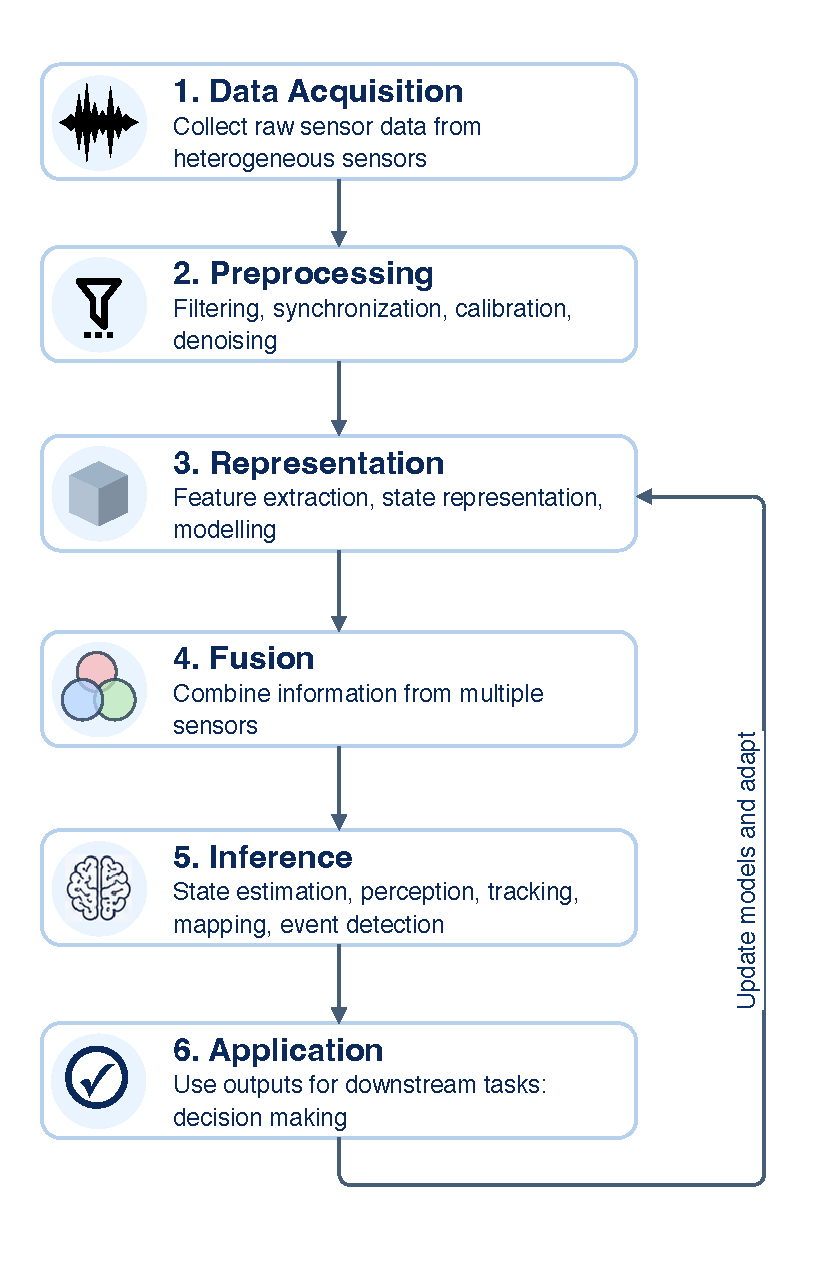
\includegraphics[width=0.85\columnwidth]{figures/fusion_pipeline_v02.pdf}
    \caption{A typical sensor fusion pipeline, from heterogeneous data acquisition to downstream application and feedback-based adaptation.}
    \label{fig:generic-sensor-fusion-pipeline}
\end{figure}

Figure~\ref{fig:generic-sensor-fusion-pipeline} summarises a generic fusion pipeline. The first stage is \emph{data acquisition}, where raw observations are collected from heterogeneous sensors or information sources. These measurements may differ in physical modality, sampling frequency, dimensionality, noise statistics, field of view, latency, and failure modes. The second stage is \emph{preprocessing}, which includes filtering, synchronisation, calibration, denoising, outlier rejection, missing-data handling, and coordinate-frame alignment. This stage is essential because fusion algorithms generally assume that measurements refer to compatible physical quantities, time instants, or spatial frames.

The third stage is \emph{representation}. Depending on the application, sensor measurements may be represented as raw signals, feature vectors, tracks, point clouds, occupancy grids, semantic objects, belief distributions, sets, or learned latent embeddings. The choice of representation strongly affects the level at which fusion is performed. Data-level fusion combines low-level measurements directly; feature-level fusion combines extracted attributes or learned representations; object-level fusion combines detections, tracks, or state estimates; and decision-level fusion combines classifier outputs, alarms, or symbolic decisions. The fourth stage is the actual \emph{fusion} step, in which information from multiple sources is combined using statistical estimation, Bayesian filtering, evidence theory, optimisation, set-membership methods, fuzzy reasoning, machine learning, or hybrid approaches.

These abstraction levels are related to the classical taxonomies of the data-fusion literature, which are worth knowing because much of that literature is organised around them. Dasarathy classifies fusion functions by the abstraction of their input and output, from \emph{data in--data out} through \emph{data in--feature out}, \emph{feature in--feature out}, and \emph{feature in--decision out} to \emph{decision in--decision out} \cite{dasarathy1997_fusion}. Durrant-Whyte classifies sensor configurations as \emph{complementary}, when the sensors observe different parts or aspects of the environment, \emph{competitive} or redundant, when they observe the same quantity and can be cross-checked, and \emph{cooperative}, when only their combination makes a quantity observable, as in stereo vision \cite{durrantwhyte1988_sensor}. The Joint Directors of Laboratories (JDL) model of the information-fusion community organises fusion functions by purpose rather than by type of data: sub-object assessment of signals and features (level~0), object assessment (level~1), situation assessment (level~2), impact or threat assessment (level~3), and process refinement (level~4), the last of which corresponds to the feedback arrow of Fig.~\ref{fig:generic-sensor-fusion-pipeline} \cite{steinberg1999_jdl}. In machine learning the same distinction between levels is expressed as \emph{early}, \emph{intermediate}, and \emph{late} fusion of modalities \cite{baltrusaitis_multimodal_2019}: early fusion corresponds to data-level fusion, intermediate fusion to feature-level fusion, and late fusion to object- and decision-level fusion; their trade-offs are compared in Table~\ref{tab:fusion-level-tradeoff} of Chapter~\ref{sec:learning}. The correspondence is approximate, because the terms are not used uniformly: in the general multimodal-learning literature, early fusion often denotes the concatenation of features already extracted from each modality \cite{baltrusaitis_multimodal_2019}, whereas the autonomous-driving literature usually reserves it for the fusion of raw or minimally processed sensor data \cite{feng2021_multimodal_survey}.


The final stages convert fused information into task-relevant knowledge. The \emph{inference} stage estimates states, detects events, tracks objects, maps environments, classifies situations, or predicts future behaviour. The \emph{application} stage then uses these outputs to support downstream tasks such as monitoring, decision-making, planning, control, diagnosis, or human assistance. The feedback arrow in Fig.~\ref{fig:generic-sensor-fusion-pipeline} highlights that practical fusion systems are rarely one-pass pipelines: outputs can be used to update models, adapt sensor weights, refine calibration, select active sensing actions, or reconfigure the system when operating conditions change.

The feedback arrow also connects the pipeline with the decision cycles studied outside the fusion literature. Boyd's observe--orient--decide--act (OODA) loop, conceived for military decision-making, describes an agent that observes its environment, orients itself by interpreting the observations in the light of prior knowledge, decides, and acts, each action changing what will be observed next \cite{boyd2018_discourse}. Read against Fig.~\ref{fig:generic-sensor-fusion-pipeline}, data acquisition and preprocessing are the observation; representation, fusion, and inference form the orientation; and the application stage decides and acts. The Omnibus model of Bedworth and O'Brien combines this cycle with the process models of the data-fusion literature \cite{bedworth2000_omnibus}: in their comparison, observation corresponds to the signal-level processing of level~0 of the JDL model, orientation to levels~1--3, and decision to process refinement (level~4), whereas action has no counterpart in the JDL model. In robotics the same cycle is called sense--plan--act, and in an automated vehicle it is the chain from perception through prediction and planning to control. For fusion the consequence is practical: the fused output is used to act, and the action determines which measurements arrive next, as when a vehicle slows down in fog or turns a steerable sensor towards an uncertain object.

\begin{figure}[!t]
    \centering
    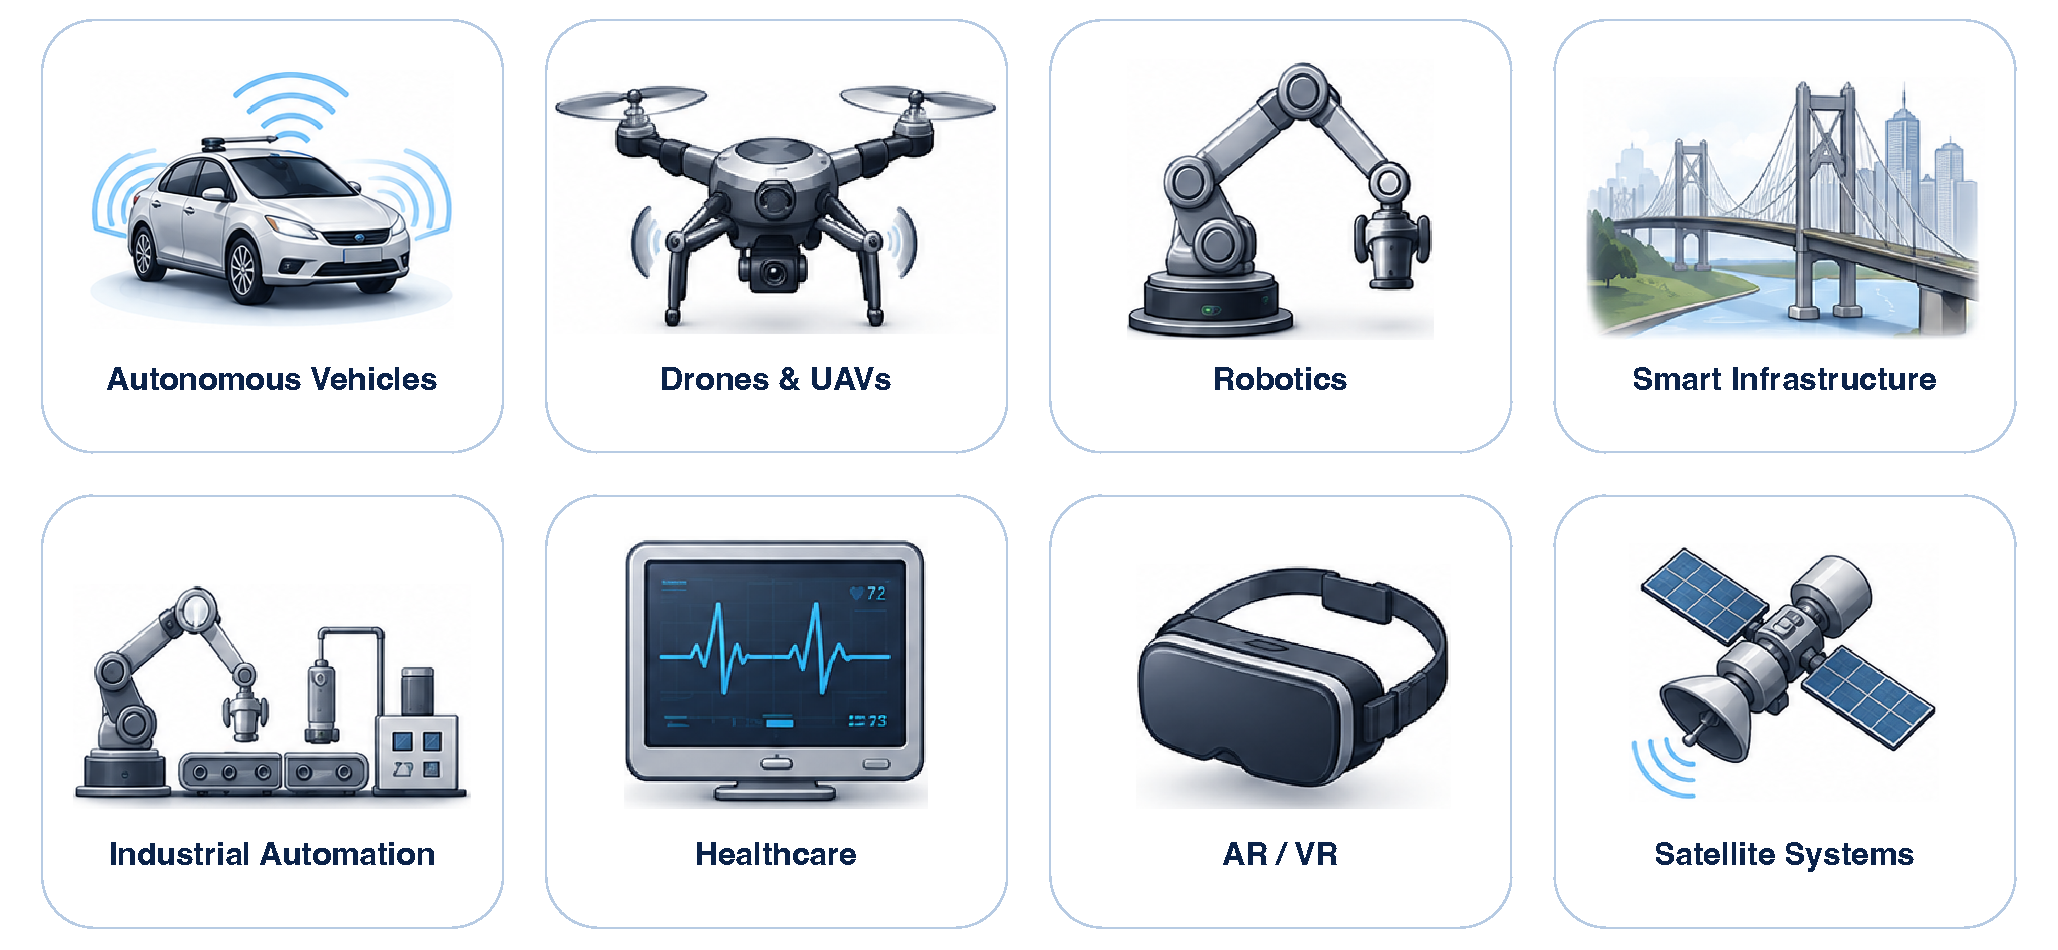
\includegraphics[width=1\columnwidth]{figures/application_areas.pdf}
    \caption{Representative application areas of sensor fusion.}
    \label{fig:application-areas}
\end{figure}

\DIFaddbegin \section{\DIFadd{Application Domains and Common Requirements}}
\DIFaddend As illustrated in Fig.~\ref{fig:application-areas}, sensor fusion is a cross-domain design pattern rather than a technique restricted to a single field. Autonomous vehicles integrate cameras, radar, LiDAR, inertial sensors, positioning systems, and maps to perceive dynamic road scenes and estimate ego-motion. Drones and unmanned aerial vehicles combine inertial, visual, GNSS, barometric, and range measurements for navigation, stabilisation, obstacle avoidance, and mapping. Robotic systems fuse proprioceptive and exteroceptive sensing to support localisation, manipulation, force control, human--robot interaction, and task planning.

Smart infrastructure combines distributed structural, environmental, traffic, and communication data to monitor bridges, roads, buildings, and energy systems. Industrial automation uses fusion to improve quality control, predictive maintenance, process monitoring, and safe collaboration between humans and machines. Healthcare systems combine physiological, imaging, wearable, and contextual data for diagnosis, monitoring, rehabilitation, and decision support. Augmented- and virtual-reality (AR/VR) systems fuse cameras, IMUs, depth sensors, eye tracking, and environmental maps to provide robust pose estimation and spatial interaction. Satellite and remote-sensing systems combine optical, radar, thermal, multispectral, and communication data to observe large-scale environmental and human activity.

Although these domains differ substantially, they share a common set of system-level requirements. First, fusion must address \emph{heterogeneity}: the input data may describe appearance, geometry, motion, range, force, acceleration, temperature, physiology, or communication events. Second, fusion must handle \emph{uncertainty}: measurements may be noisy, ambiguous, delayed, intermittent, biased, or contradictory. Third, fusion must satisfy \emph{operational constraints}: many applications require real-time or near-real-time performance on embedded or distributed hardware. Fourth, fusion must support \emph{robustness}: safety-critical systems must continue operating under sensor degradation, environmental changes, communication losses, and out-of-distribution conditions. These requirements explain why the field contains both model-based methods, which provide explicit uncertainty handling and interpretability, and learning-based methods, which provide rich representations for complex multimodal data.

\DIFaddbegin \section{\DIFadd{System Components and Outputs}}
\DIFaddend From a design perspective, the main components of a sensor fusion system can therefore be summarised as follows:
\begin{list4a}
    \item \textbf{Sensing sources}: physical sensors, virtual sensors, maps, communication messages, historical data, and model predictions that provide partial information about the system or environment.
    \item \textbf{Temporal and spatial alignment}: synchronisation, interpolation, latency compensation, intrinsic calibration, extrinsic calibration, and coordinate transformations that make heterogeneous data comparable.
    \item \textbf{Representation and abstraction level}: raw measurements, engineered features, learned embeddings, detections, tracks, occupancy maps, semantic maps, probability distributions, bounded sets, or decisions.
    \item \textbf{Uncertainty and reliability modelling}: probabilistic noise models, confidence scores, belief masses, fuzzy memberships, deterministic bounds, sensor-health indicators, and context-dependent reliability weights.
    \item \textbf{Fusion mechanism}: algorithms or architectures that combine information, resolve conflicts, exploit complementarity, handle redundancy, and propagate uncertainty to later stages.
    \item \textbf{Inference and downstream use}: state estimation, perception, tracking, mapping, event detection, prediction, planning, control, monitoring, diagnosis, or decision support.
    \item \textbf{Adaptation and validation}: mechanisms for online model update, failure detection, recalibration, robustness assessment, uncertainty calibration, and verification under representative and rare operating conditions.
\end{list4a}

This system-level view motivates the organisation of the rest of the book. Chapter~\ref{sec:classicalSF} first reviews classical fusion techniques, including probabilistic, statistical, evidence-theoretic, optimisation-based, and set-membership approaches. Chapter~\ref{sec:learning} then examines learning-based and hybrid techniques, where multimodal representations are learned directly from data and combined with model-based estimation or decision-making. Throughout the book, autonomous driving is used as a concrete reference domain, while the underlying principles remain applicable to the broader application areas shown in Fig.~\ref{fig:application-areas}.

\begin{figure}[!t]
    \centering
    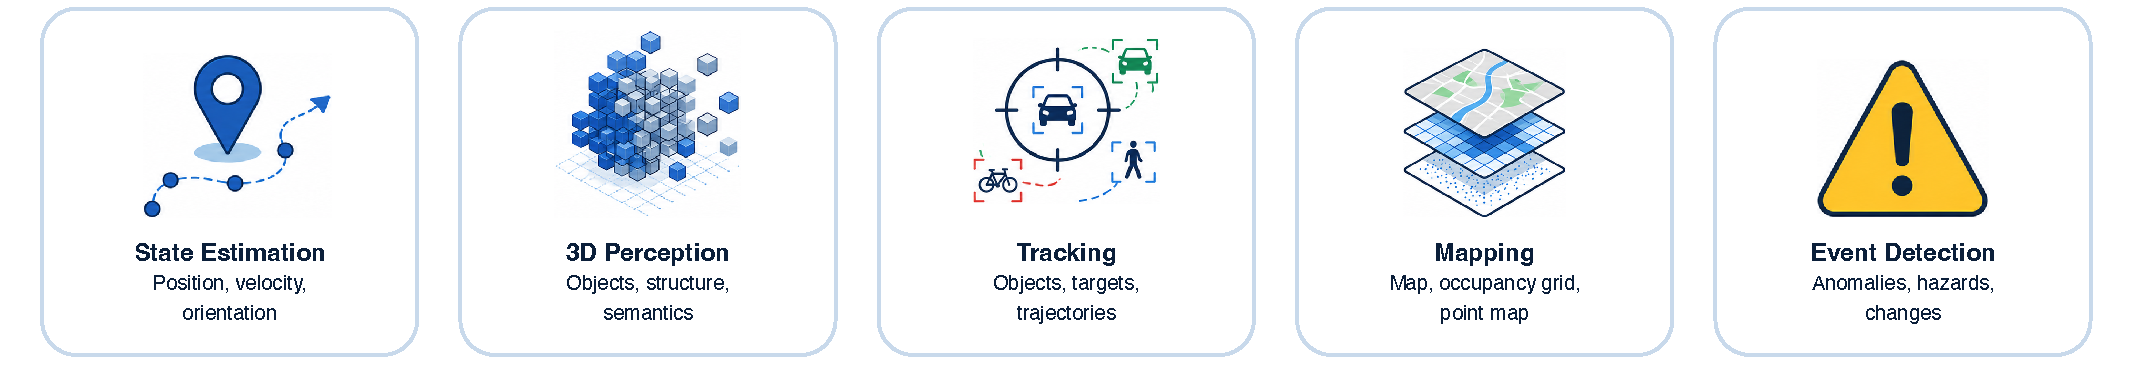
\includegraphics[width=1\columnwidth]{figures/estimates_outputs.pdf}
    \caption{Representative outputs produced by sensor-fusion systems, ranging from state estimates and tracks to maps, decisions, and uncertainty-aware alerts.}
    \label{fig:estimates-outputs}
\end{figure}

Figure~\ref{fig:estimates-outputs} emphasises that the output of a fusion system is not limited to a single point estimate. Depending on the application and abstraction level, fusion may produce filtered state estimates, covariance matrices, bounded state sets, object tracks, occupancy maps, semantic labels, anomaly scores, conflict indicators, reliability weights, or control-relevant decisions. These outputs should be interpreted together with their uncertainty and validity assumptions. For example, a vehicle pose estimate is useful only when accompanied by a covariance, confidence interval, or bounded error envelope; an object detection becomes more valuable when associated with a track identity and existence confidence; and a decision-level alert is safer when it exposes whether sensors agree, disagree, or are degraded. This motivates the transition from system components to the classical mathematical tools reviewed in the next section.

The \DIFdelbegin \DIFdel{component view of this chapter is also the key to the end-of-chapter problems of the following chapters . Each problem isolates one component of the pipeline, such as the weighting of two sourcesof different accuracy, the alignment of a delayed track, the propagation of a bounded set, or the resolution of a conflictbetween two classifiers, and asks the reader to carry out the corresponding computation by hand or with the companion repository. Reading a problem, it is therefore useful to ask first which block of }\DIFdelend \DIFaddbegin \DIFadd{exercises in later chapters isolate these components: weighting sources, aligning delayed tracks, propagating bounded sets, or resolving conflict. Before calculating, identify the pipeline block in }\DIFaddend Fig.~\ref{fig:generic-sensor-fusion-pipeline} \DIFdelbegin \DIFdel{it exercises and which of the outputs of }\DIFdelend \DIFaddbegin \DIFadd{and the output in }\DIFaddend Fig.~\ref{fig:estimates-outputs}\DIFdelbegin \DIFdel{it produces. The solutions collected at the end of the book return to this question explicitly whenever a numerical result has a }\DIFdelend \DIFaddbegin \DIFadd{. Interpret each numerical answer in terms of that }\DIFaddend system-level \DIFdelbegin \DIFdel{interpretation}\DIFdelend \DIFaddbegin \DIFadd{role}\DIFaddend .






\clearpage

\clearpage

\chapter{Classical Sensor Fusion Techniques}
\label{sec:classicalSF}








\abstract{This chapter reviews the classical, model-based techniques of sensor fusion, and presents them as variations of a single idea: measurements are pieces of information about a hidden state, to be weighted by their uncertainty and combined additively when they are independent. The chapter starts from the static inverse problem and develops ordinary, weighted, regularised and sequential least squares, their maximum-likelihood and maximum-a-posteriori interpretations, the information matrix, and Gauss--Newton iterations for nonlinear sensor models. The same prediction--correction structure is then extended to dynamic states through Bayesian filtering, covering the Kalman filter, the extended and unscented Kalman filters (EKF, UKF), particle filters, innovation-based gating and the normalised innovation squared as a consistency diagnostic; a worked automotive-radar cut-in example with real numbers accompanies the discussion. Set-membership and zonotopic estimation are presented as the bounded-error counterpart of probabilistic filtering, with strip intersections, order reduction and a direct comparison with the EKF on the same scenario. Track-level fusion and data association follow, including temporal and spatial alignment, gating, nearest-neighbour, probabilistic and multi-hypothesis association, track management, fusion with known cross-correlation and covariance intersection. Evidence theory (Dempster--Shafer, the transferable belief model and Dezert--Smarandache theory, DSmT) is introduced for conflicting qualitative information, optimisation-based fusion and factor graphs for trajectory estimation, and multi-criteria decision-making, in particular the incomplete Analytic Hierarchy Process (AHP) solved by logarithmic least squares, for context-dependent sensor reliability weighting. The chapter closes with ten problems, whose solutions are collected at the end of the book and in the companion repository.}
\suppressfloats[t]

\section{Mathematical introduction to sensor fusion}
\label{sec:math-intro}


Sensor fusion concerns the estimation of an unknown physical quantity from multiple measurements that may differ in modality, dimension, accuracy, sampling rate, and uncertainty. The quantity to be estimated may be a static parameter, such as the location of a stationary source, or a time-varying state, such as the position, velocity, and orientation of a moving vehicle. Table~\ref{tab:notation} collects the notation used throughout the book and records where symbols are reused with different meanings across the method families reviewed here.
\begin{table}[!t]
    \centering
    \renewcommand{\arraystretch}{1.25}
    \small
    \caption{Principal notation. Symbols are reused across method families where the literatures conflict; the scope column states where each reading applies.}
    \label{tab:notation}
    \begin{tabular}{p{0.13\linewidth} p{0.44\linewidth} p{0.28\linewidth}}
        \hline
        \textbf{Symbol} & \textbf{Meaning} & \textbf{Scope} \\
        \hline
        $\mathbf{x}$, $\widehat{\mathbf{x}}$ & state, estimate & throughout \\
        $\mathbf{y}$, $\mathbf{r}$ & measurement, measurement noise & throughout \\
        $\mathbf{g}(\cdot)$, $\mathbf{G}$ & measurement function, measurement matrix & throughout \\
        $\mathbf{f}(\cdot)$, $\mathbf{q}$ & process model, process noise & dynamic models \\
        $\mathbf{R}$, $\mathbf{Q}$, $\mathbf{P}$ & measurement, process, state covariance & probabilistic fusion \\
        $\mathbf{\Lambda}$ & information matrix, $\mathbf{P}^{-1}$ & probabilistic fusion \\
        $\boldsymbol{\nu}$, $\mathbf{S}$, $\mathbf{K}$ & innovation, its covariance, gain & filtering \\
        $\mathbf{m}$ & prior mean & regularised least squares \\
        $p$, $H$, $\gamma$ & zonotope centre, generators, strip gain & set-membership \\
        $\Omega$, $m(\cdot)$, $K$ & frame of discernment, belief mass, conflict & evidence theory \\
        $w$, $q$, $\mu$ & fusion weight, quality indicator, membership & reliability-aware fusion \\
        $\mathcal{G}$, $\mathcal{N}_i$ & communication graph, neighbour set & multi-agent fusion \\
        $\mathbf{H}$ & measurement Jacobian or matrix inside filtering recursions (equals $\mathbf{G}$ for linear models) & Kalman filtering, Chapters~\ref{sec:learning}--\ref{sec:applications} \\
        $\mathbf{L}$, $\lambda_2$, $\epsilon$ & graph Laplacian, algebraic connectivity, consensus step size & multi-agent fusion \\
        $\alpha_i$ & discount (reliability) factor applied to the evidence of source $i$ & evidence theory, reliability-aware fusion \\
        NIS, NEES & normalised innovation squared, normalised estimation error squared (consistency statistics) & filtering, validation \\
        ECE, $T$ & expected calibration error, temperature-scaling parameter & learning-based fusion \\
        $\mathbf{f}_c$, $\mathbf{f}_l$, $\mathbf{f}_r$ & camera, LiDAR, radar feature representations & deep multimodal fusion \\
        $\mathbf{T}_{VS}$, $\mathbf{K}$ & extrinsic sensor-to-vehicle transform in $SE(3)$; camera intrinsic matrix (the gain is written $\mathbf{K}_k$ when both appear) & calibration and alignment, Chapter~\ref{sec:application} \\
        $\mathbf{\Omega}_i$ & information matrix of the $i$-th factor in factor-graph and SLAM formulations (bold, unrelated to the frame of discernment $\Omega$) & factor graphs, Chapter~\ref{sec:learning} \\
        \hline
    \end{tabular}
\end{table}

Readers trained in machine learning or computer science will meet most objects of this chapter under other names, because the estimation and the machine-learning literatures describe the same probabilistic models from different starting points \cite{bishop2006_prml,koller2009_pgm,sarkka2013_bayesian}. Table~\ref{tab:ml-dictionary} gives the correspondence for the main concepts of this and the following chapters. The letters differ as well: the machine-learning literature usually denotes the latent state by $\mathbf{z}$ and the observation by $\mathbf{x}$ \cite{bishop2006_prml}, whereas this book follows the convention of estimation and control, with $\mathbf{x}$ for the state and $\mathbf{y}$ for the measurement. Some entries are exact identities: the Kalman filter is exact inference in a linear-Gaussian state-space model, that is, in a hidden Markov model with continuous states, and the regularised least-squares estimate with a Gaussian prior is ridge regression. Others are analogies that help intuition: zonotopes are also an abstract domain for the static analysis of programs and for the verification of neural networks \cite{ghorbal2009_zonotope,gehr2018_ai2}; the logarithmic least-squares completion of an incomplete AHP matrix is a least-squares ranking on a comparison graph, closely related to HodgeRank and to the Bradley--Terry model \cite{jiang2011_hodgerank,bradley1952_paired}; and the resilient consensus of Chapter~\ref{sec:MAS} belongs to the same family as the Byzantine-robust aggregation rules of distributed learning \cite{yin2018_byzantine}.

\begin{table}[!t]
    \centering
    \footnotesize
    \setlength{\tabcolsep}{4pt}
    \renewcommand{\arraystretch}{1.3}
    \caption{The main objects of this book in the vocabulary of machine learning and computer science.}
    \label{tab:ml-dictionary}
    \begin{tabular}{>{\raggedright\arraybackslash}p{0.33\linewidth} >{\raggedright\arraybackslash}p{0.44\linewidth} >{\raggedright\arraybackslash}p{0.14\linewidth}}
        \hline
        \textbf{Estimation and fusion} & \textbf{Machine learning and computer science} & \textbf{In this book} \\
        \hline
        state $\mathbf{x}$ & latent (hidden) variable & Sect.~\ref{sec:math-intro} \\
        measurement model $\mathbf{g}(\cdot)$ with noise $\mathbf{r}$ & observation model, likelihood $p(\mathbf{y}\mid\mathbf{x})$; decoder of a generative model & Sect.~\ref{sec:math-intro} \\
        process model $\mathbf{f}(\cdot)$ with noise $\mathbf{q}$ & transition model $p(\mathbf{x}_k\mid\mathbf{x}_{k-1})$ & Sect.~\ref{sec:bayes-filtering} \\
        (weighted) least squares; maximum-likelihood estimate under Gaussian noise & (weighted) mean-squared-error regression; minimisation of the negative log-likelihood & Sect.~\ref{sec:math-intro} \\
        regularised least squares; maximum a posteriori (MAP) estimate with Gaussian prior & ridge (Tikhonov, $\ell_2$) regularisation, the prior acting as regulariser & Sect.~\ref{sec:math-intro} \\
        information matrix $\mathbf{\Lambda}$ & precision matrix (inverse covariance); Fisher information; Hessian of the negative log-likelihood & Sect.~\ref{sec:math-intro} \\
        sequential least squares & recursive least squares; online learning & Sect.~\ref{sec:math-intro} \\
        Bayesian filter (prediction and update) & forward recursion of inference in a hidden Markov model or dynamic Bayesian network & Sect.~\ref{sec:bayes-filtering} \\
        Kalman filter & exact inference in a linear-Gaussian state-space model (linear dynamical system) & Sect.~\ref{sec:bayes-filtering} \\
       extended and unscented Kalman filters (EKF, UKF) & approximate inference by linearisation and by deterministic sampling & Sect.~\ref{sec:bayes-filtering} \\
       observability of the state & identifiability of the latent variables from the observations & Chapters~\ref{sec:application} and~\ref{sec:MAS} \\
        particle filter & sequential Monte Carlo (sequential importance resampling) & Sect.~\ref{sec:bayes-filtering} \\
        innovation $\boldsymbol{\nu}$, NIS test & prediction residual; calibration and out-of-distribution test on residuals & Sect.~\ref{sec:bayes-filtering} \\
        zonotopic set-membership estimate & reachability analysis; zonotope abstract domain of program analysis and neural-network verification & Sect.~\ref{sec:set-membership} \\
        gating and data association & outlier rejection; bipartite matching (assignment problem) & Sect.~\ref{sec:track-level} \\
        covariance intersection & conservative aggregation of estimates with unknown dependence, avoiding double counting & Sect.~\ref{subsec:track-fusion} \\
        belief masses, Dempster's rule & belief functions; second-order uncertainty in classification, as in evidential deep learning \cite{sensoy2018_edl} & Sect.~\ref{sec:evidence} \\
        factor graph & probabilistic graphical model \cite{kschischang2001_factor}; sparse nonlinear least squares & Sect.~\ref{sec:factor-graphs} \\
        incomplete AHP, logarithmic least squares & ranking from pairwise comparisons (HodgeRank, Bradley--Terry) & Sect.~\ref{sec:mcdm} \\
        learned measurement covariance & heteroscedastic regression; uncertainty calibration & Chapter~\ref{sec:learning} \\
        consensus; resilient (W-MSR) consensus & gossip averaging \cite{boyd2006_gossip}; Byzantine-robust aggregation & Chapter~\ref{sec:MAS} \\
        \hline
    \end{tabular}
\end{table}







\subsection{Sensor fusion as an inverse problem}

Let $\mathbf{x}\in\mathbb{R}^{d_x}$ denote the unknown state or parameter vector. The $n$-th sensor measurement is modelled as
\begin{align}
\mathbf{y}_n=\mathbf{g}_n(\mathbf{x})+\mathbf{r}_n, \qquad n=1,\ldots,N,
\end{align}
where $\mathbf{y}_n\in\mathbb{R}^{d_n}$ is the observed measurement, $\mathbf{g}_n:\mathbb{R}^{d_x}\rightarrow\mathbb{R}^{d_n}$ is the measurement or observation function of sensor $n$, and $\mathbf{r}_n\in\mathbb{R}^{d_n}$ represents measurement noise and modelling error.

The sensor-fusion problem is therefore an inverse problem: the forward models $\mathbf{g}_n(\cdot)$ describe how a hypothetical state produces measurements, while fusion attempts to infer the state that most plausibly explains the measurements actually observed. 

Different sensors need not measure the state directly. For example, a GNSS receiver may provide a noisy position measurement,
\begin{align*}
\mathbf{y}_{\mathrm{GNSS}}=\mathbf{p}+\mathbf{r}_{\mathrm{GNSS}},
\end{align*}
whereas a range sensor located at $\mathbf{s}_n$ may provide
\begin{align*}
y_n=\left\|\mathbf{p}-\mathbf{s}_n\right\|_2+r_n.
\end{align*}
A camera may instead provide a perspective projection,
\begin{align*}
\Pi\left(\boldsymbol{\mathcal{R}}\,\mathbf{p}+\mathbf{t}\right) +\mathbf{r}_n,
\end{align*}
where $\Pi(\cdot)$ is a nonlinear projection operator and $\boldsymbol{\mathcal{R}}$ is a rotation matrix. Sensor fusion places all such measurements within a common estimation framework despite their different physical interpretations.


\subsection{Measurement uncertainty}

Measurements are not exact. Their uncertainty can arise from thermal noise, quantisation, imperfect calibration, environmental interference, finite resolution, unmodelled dynamics, or errors in the assumed sensor model.

A standard starting assumption is that the measurement error has zero mean, $\mathbb{E}[\mathbf{r}_n]=\mathbf{0}_{d_n}$, and covariance $\mathbf{R}_n\in\mathbb{R}^{d_n\times d_n}$. The covariance matrix $\mathbf{R}_n$ describes both the magnitude and the directional structure of the uncertainty. For a scalar measurement, $y_n=g_n(\mathbf{x})+r_n$, the covariance reduces to the variance $\operatorname{var}(r_n)=\sigma_n^2$. A larger $\sigma_n^2$ means that the measurement is less precise. Figure~\ref{fig:mean-variance}(a) illustrates both notions: when the error has zero mean, repeated readings of the same quantity scatter around its true value, and the width of the scatter, measured by the standard deviation $\sigma_n$, is larger for the less precise sensor. For a vector measurement $\mathbf{y}\triangleq \begin{bmatrix} y_{1} & y_{2} & \cdots & y_{d_n} \end{bmatrix}^T \in \mathbb{R}^{d_n}$,
\begin{align*}
\mathbf{R}=
\begin{bmatrix}
\operatorname{var}(r_{1}) & \operatorname{cov}(r_{1},r_{2}) & \cdots & \operatorname{cov}(r_{1},r_{d_n})\\
\operatorname{cov}(r_{2},r_{1}) & \operatorname{var}(r_{2}) & \cdots & \operatorname{cov}(r_{2},r_{d_n}) \\
\vdots & \vdots & \ddots & \vdots\\
\operatorname{cov}(r_{d_n},r_{1})  & \operatorname{cov}(r_{d_n},r_{2}) & \cdots & \operatorname{var}(r_{d_n}) \\
\end{bmatrix},
\end{align*}
the diagonal entries represent component-wise variances, while the off-diagonal entries represent correlations between measurement components. When the off-diagonal terms are non-zero, the measurement components are correlated, and the uncertainty region is tilted with respect to the coordinate axes. An eigenvalue decomposition removes the tilt by rotating into the axes along which the errors are uncorrelated. For a two-dimensional position measurement
the correlated uncertainty region then becomes an ellipse,

\begin{align*}
\mathbf{R}=\mathbf{U}\left[\begin{matrix}\lambda _{1}&0\\ 0&\lambda _{2}\end{matrix}\right]\mathbf{U}^{\mathsf{T}} \;.
\end{align*}
In this decoupled form, the eigenvectors in $\mathbf{U}$ serve as a rotation matrix that determines the principal axes (directions) of the uncertainty ellipse. Meanwhile, the eigenvalues $\lambda _{1}$ and $\lambda _{2}$ represent the decoupled variances, directly dictating the lengths (magnitudes) of the ellipse's semi-axes along those new directions: for the ellipse of one standard deviation the semi-axes are $\sqrt{\lambda_1}$ and $\sqrt{\lambda_2}$, as shown in Fig.~\ref{fig:mean-variance}(b).

\begin{figure}[!t]
\centering
\resizebox{\columnwidth}{!}{
\begin{tikzpicture}
\begin{groupplot}[
    group style={group size=2 by 1, horizontal sep=16mm},
    scale only axis,
    tick label style={font=\scriptsize},
    label style={font=\scriptsize},
    title style={font=\scriptsize, yshift=0.5mm},
    axis line style={line width=0.5pt},
    tick align=outside,
]

\nextgroupplot[
    width=0.42\columnwidth, height=3.3cm,
    xlabel={reading [m]},
    xmin=8.3, xmax=11.3, ymin=-0.45, ymax=1.7,
    ytick={0,1}, yticklabels={coarse, precise},
    title={(a) repeated readings of a $10$\,m distance},
]
\addplot[draw=gray!60, dashed, line width=0.4pt, forget plot] coordinates {(10,-0.45) (10,1.7)};
\addplot[only marks, mark=*, mark size=0.9pt, draw=EkfBlue, fill=EkfBlue]
    table[x=a, y=ja, col sep=comma] {data/ch03/mean_variance_1d.csv};
\addplot[only marks, mark=square*, mark size=0.8pt, draw=ManoeuvreOrange!80!black, fill=ManoeuvreOrange!80!black]
    table[x=b, y=jb, col sep=comma] {data/ch03/mean_variance_1d.csv};

\draw[EkfBlue, line width=0.7pt, |-|] (axis cs:9.757,1.36) -- (axis cs:10.227,1.36);
\fill[EkfBlue] (axis cs:9.992,1.36) circle (1.5pt);
\draw[ManoeuvreOrange!80!black, line width=0.7pt, |-|] (axis cs:9.298,0.36) -- (axis cs:10.524,0.36);
\fill[ManoeuvreOrange!80!black] (axis cs:9.911,0.36) circle (1.5pt);
\node[font=\scriptsize, anchor=west] at (axis cs:10.27,1.36) {$\bar y\pm s$};
\node[font=\scriptsize, anchor=west] at (axis cs:10.57,0.36) {$\bar y\pm s$};

\nextgroupplot[
    width=0.42\columnwidth, height=3.3cm,
    axis equal image,
    xlabel={east error $r_1$ [m]}, ylabel={north error $r_2$ [m]},
    xmin=-3.3, xmax=3.3, ymin=-2.3, ymax=2.3,
    title={(b) correlated two-dimensional errors},
]
\addplot[only marks, mark=*, mark size=0.45pt, draw=MeasGrey, fill=MeasGrey]
    table[x=x, y=y, col sep=comma] {data/ch03/covariance_2d_samples.csv};
\addplot[EkfBlue, line width=0.9pt]
    table[x=x1, y=y1, col sep=comma] {data/ch03/covariance_2d_ellipses.csv};
\draw[->, >=stealth, line width=0.8pt, TruthBlack] (axis cs:0,0) -- (axis cs:0.9845,0.6563);
\draw[->, >=stealth, line width=0.8pt, TruthBlack] (axis cs:0,0) -- (axis cs:-0.1754,0.2631);
\node[font=\scriptsize, anchor=west, inner sep=1pt, fill=white, fill opacity=0.85, text opacity=1] at (axis cs:1.35,0.15) {$\sqrt{\lambda_1}\,\mathbf{u}_1$};
\draw[gray, line width=0.3pt] (axis cs:1.37,0.22) -- (axis cs:0.75,0.50);
\node[font=\scriptsize, anchor=east, inner sep=1pt, fill=white, fill opacity=0.85, text opacity=1] at (axis cs:-0.95,1.25) {$\sqrt{\lambda_2}\,\mathbf{u}_2$};
\draw[gray, line width=0.3pt] (axis cs:-0.97,1.18) -- (axis cs:-0.15,0.30);
\end{groupplot}
\end{tikzpicture}}
\caption{Mean, variance, and covariance of measurement errors. (a) Forty readings of the same $10$\,m distance (dashed line) taken by a precise sensor ($\sigma=0.2$\,m, dots) and by a coarse one ($\sigma=0.6$\,m, squares); the vertical scatter only separates overlapping marks. The bars show the sample mean $\bar y=\frac{1}{M}\sum_{j=1}^{M}y_j$ and one sample standard deviation $s=\big(\frac{1}{M-1}\sum_{j=1}^{M}(y_j-\bar y)^2\big)^{1/2}$ on each side, with $M=40$: $\bar y=9.99$ and $9.91$\,m, $s=0.24$ and $0.61$\,m. Both sets scatter around the true value, the coarse one about three times more widely. (b) Three hundred samples of a two-dimensional error with covariance $\mathbf{R}=\left[\begin{smallmatrix}1.0&0.6\\0.6&0.5\end{smallmatrix}\right]$\,m$^2$ (correlation coefficient $0.85$). The ellipse is the set of points $\mathbf{r}$ with $\mathbf{r}^{\mathsf T}\mathbf{R}^{-1}\mathbf{r}=1$: its principal axes are the eigenvectors $\mathbf{u}_1,\mathbf{u}_2$ of $\mathbf{R}$, and its semi-axes are $\sqrt{\lambda_1}=1.18$\,m and $\sqrt{\lambda_2}=0.32$\,m, with $\lambda_1=1.4$ and $\lambda_2=0.1$\,m$^2$. Data generated by \repopath{companion\_\allowbreak repo/\allowbreak examples/\allowbreak ch03\_mean\_variance\_gaussian/}.}
\label{fig:mean-variance}
\end{figure}



\subsection{Independent and correlated measurement errors}

A common simplifying assumption is that the errors of different measurements are mutually independent. Under this assumption, measurements may have different covariance matrices, but their errors do not share common random components. Independence is reasonable when measurements arise from physically separate noise processes. It may be violated, however, when sensors share calibration parameters, environmental disturbances, timing errors, communication links, or preprocessing algorithms. For example, two position estimates derived from the same camera images generally have correlated errors. Likewise, repeated measurements from the same biased sensor may be strongly correlated even when their high-frequency noise samples are independent. The distinction is important because treating correlated measurements as independent effectively counts shared information more than once, causing an estimator to become overconfident\footnote{The intuition is simple: if two sensors share a common disturbance, calibration error, map error, timing error, or modelling error, then their mistakes tend to point in the same direction. Seeing both sensors agree does not mean the estimate is twice as reliable. They may agree because they are affected by the same hidden error.}.

Mathematically, the absence of correlation between two different measurement errors can be described through their cross-covariance. For measurements indexed by $m$ and $n$, this cross-covariance is defined as
\begin{equation}
\operatorname{cov}(\mathbf{r}_m,\mathbf{r}_n) = \mathbb{E}\left[\left(\mathbf{r}_m-\mathbb{E}[\mathbf{r}_m]\right)\left(\mathbf{r}_n-\mathbb{E}[\mathbf{r}_n]\right)^{\mathsf T}\right].
\end{equation}
Thus, the assumption that different measurement errors are uncorrelated is written as
\begin{equation}
\operatorname{cov}(\mathbf{r}_m,\mathbf{r}_n) = \mathbf{0}, \quad m\neq n.
\end{equation}
It is useful to distinguish between being uncorrelated and being independent. Independence implies zero cross-covariance, provided the covariance exists. The reverse is not true in general. However, when the errors are jointly Gaussian, zero cross-covariance is sufficient to imply independence. This is one reason why Gaussian models are especially convenient in sensor fusion.


\subsection{Stacked measurement model}

Writing all measurements in a common stacked form turns the fusion of $N$ sensors into the processing of a single, longer measurement vector, so that the formulas derived below do not depend on how many sensors there are. Starting from the individual measurement models
\begin{equation}
\mathbf{y}_n
=
\mathbf{g}_n(\mathbf{x})
+
\mathbf{r}_n,
\qquad n=1,\ldots,N,
\end{equation}
we define the stacked measurement vector as
\begin{equation}
\underbrace{\begin{bmatrix}
\mathbf{y}_1\\
\mathbf{y}_2\\
\vdots\\
\mathbf{y}_N
\end{bmatrix}}_{\triangleq \mathbf{y}} = 
\underbrace{\begin{bmatrix}
\mathbf{g}_1(\mathbf{x})\\
\mathbf{g}_2(\mathbf{x})\\
\vdots\\
\mathbf{g}_N(\mathbf{x})
\end{bmatrix}}_{\triangleq \mathbf{g}(\mathbf{x})} + 
\underbrace{\begin{bmatrix}
\mathbf{r}_1\\
\mathbf{r}_2\\
\vdots\\
\mathbf{r}_N
\end{bmatrix}.}_{\triangleq \mathbf{r}}
\end{equation}
This compact representation is important because it allows heterogeneous measurements to be handled in a unified way. The entries of $\mathbf{y}$ may include positions, velocities, accelerations, ranges, bearings, pixel coordinates, signal strengths, or other sensor outputs. The role of $\mathbf{g}(\mathbf{x})$ is to predict, for a given candidate state $\mathbf{x}$, what each sensor should observe.

The covariance of the stacked noise vector is
\begin{equation}
\mathbf{R}
\triangleq
\operatorname{cov}(\mathbf{r}) = \mathbb{E} \left[ \left( \mathbf{r}-\mathbb{E}[\mathbf{r}] \right) \left( \mathbf{r}-\mathbb{E}[\mathbf{r}] \right)^{\mathsf T} \right].
\end{equation}
If the measurement errors are mutually uncorrelated, then the covariance matrix has the block-diagonal structure
\begin{equation}
\mathbf{R}=
\begin{bmatrix}
\mathbf{R}_1 & \mathbf{0} & \cdots & \mathbf{0}\\
\mathbf{0} & \mathbf{R}_2 & \cdots & \mathbf{0}\\
\vdots & \vdots & \ddots & \vdots\\
\mathbf{0} & \mathbf{0} & \cdots & \mathbf{R}_N
\end{bmatrix}.
\end{equation}
If the measurement errors are correlated, the covariance matrix instead contains nonzero off-diagonal blocks:
\begin{equation}
\mathbf{R}
=
\begin{bmatrix}
\mathbf{R}_{11} & \mathbf{R}_{12} & \cdots & \mathbf{R}_{1N}\\
\mathbf{R}_{21} & \mathbf{R}_{22} & \cdots & \mathbf{R}_{2N}\\
\vdots & \vdots & \ddots & \vdots\\
\mathbf{R}_{N1} & \mathbf{R}_{N2} & \cdots & \mathbf{R}_{NN}
\end{bmatrix}.
\end{equation}
The diagonal block $\mathbf{R}_{nn}$ describes the uncertainty of the $n$th measurement, while the off-diagonal block $\mathbf{R}_{mn}$ is
\begin{equation}
\mathbf{R}_{mn} = \operatorname{cov}(\mathbf{r}_m,\mathbf{r}_n).
\end{equation}
These off-diagonal terms should not be ignored when sensors share common sources of uncertainty. If they are ignored, the estimator may behave as if more independent information is available than there really is.


\subsection{Gaussian measurement model}

A common and analytically convenient assumption is that the stacked measurement noise is Gaussian, i.e., $\mathbf{r} \sim \mathcal{N} \left( \mathbf{0}, \mathbf{R} \right)$. Since the measurement model is $\mathbf{y}=\mathbf{g}(\mathbf{x})+\mathbf{r}$, the conditional distribution of the measurements given the state is $\mathbf{y}\mid\mathbf{x} \sim \mathcal{N} \left( \mathbf{g}(\mathbf{x}), \mathbf{R} \right)$. 
The corresponding likelihood is
\begin{equation}
\label{eq:Gaussianlikelihood}
p(\mathbf{y}\mid\mathbf{x}) = \frac{1}{(2\pi)^{d_y/2}|\mathbf{R}|^{1/2}}\exp \left( - \frac{1}{2} \left( \mathbf{y}-\mathbf{g}(\mathbf{x})\right)^{\mathsf T}\mathbf{R}^{-1}\left(\mathbf{y}-\mathbf{g}(\mathbf{x})\right)\right),
\end{equation}
where $d_y$ is the dimension of the stacked measurement vector. This expression shows that the plausibility of a state is not determined by the residual alone, but by the residual relative to the uncertainty. A residual of a given numerical size may be significant for a precise sensor and insignificant for a noisy sensor.

Figure~\ref{fig:gaussian-1d-2d} shows the Gaussian density in one and two dimensions. For a scalar measurement, the interval of one standard deviation around the mean contains $68.3\,\%$ of the probability, and the interval of two standard deviations contains $95.4\,\%$. For a vector measurement, the density is constant on the ellipses (ellipsoids, in more than two dimensions) on which the quadratic form in the exponent of \eqref{eq:Gaussianlikelihood} takes a constant value $c^2$; their principal axes are the eigenvectors of $\mathbf{R}$ and their semi-axes are $c\sqrt{\lambda_1}$ and $c\sqrt{\lambda_2}$. The quadratic form is the squared Mahalanobis distance of the residual, that is, its squared length measured in units of the noise covariance, and for a Gaussian residual it follows a chi-square distribution with $d_y$ degrees of freedom. The probability contained in an ellipse therefore depends on the dimension: for $d_y=2$ it equals $1-e^{-c^2/2}$, which is only $39.3\,\%$ for $c=1$ and $86.5\,\%$ for $c=2$. The one-standard-deviation intuition of the scalar case does not carry over to several dimensions; the same chi-square distribution provides the thresholds of the consistency tests and of the gates of Sects.~\ref{sec:bayes-filtering} and~\ref{sec:track-level}.

\begin{figure}[!t]
\centering
\resizebox{\columnwidth}{!}{
\begin{tikzpicture}
\begin{groupplot}[
    group style={group size=2 by 1, horizontal sep=16mm},
    scale only axis,
    tick label style={font=\scriptsize},
    label style={font=\scriptsize},
    title style={font=\scriptsize, yshift=0.5mm},
    axis line style={line width=0.5pt},
    tick align=outside,
]

\nextgroupplot[
    width=0.42\columnwidth, height=3.3cm,
    xmin=-3.6, xmax=3.6, ymin=0, ymax=0.56,
    xtick={-3,-2,-1,0,1,2,3},
    xlabel={standardised value $(y-\mu)/\sigma$},
    ytick=\empty, ylabel={density},
    axis x line=bottom, axis y line=left,
    title={(a) scalar Gaussian density},
]
\addplot[draw=none, fill=EkfBlue!14, domain=-2:2, samples=61] {exp(-x^2/2)/sqrt(2*pi)} \closedcycle;
\addplot[draw=none, fill=EkfBlue!35, domain=-1:1, samples=41] {exp(-x^2/2)/sqrt(2*pi)} \closedcycle;
\addplot[TruthBlack, line width=0.9pt, domain=-3.6:3.6, samples=121] {exp(-x^2/2)/sqrt(2*pi)};
\draw[<->, >=stealth, line width=0.5pt] (axis cs:-1,0.435) -- (axis cs:1,0.435)
    node[midway, above, font=\scriptsize, inner sep=1pt] {$68.3\,\%$};
\draw[<->, >=stealth, line width=0.5pt] (axis cs:-2,0.505) -- (axis cs:2,0.505)
    node[midway, above, font=\scriptsize, inner sep=1pt] {$95.4\,\%$};

\nextgroupplot[
    width=0.42\columnwidth, height=3.3cm,
    axis equal image,
    xlabel={$r_1$ [m]}, ylabel={$r_2$ [m]},
    xmin=-3.6, xmax=3.6, ymin=-2.5, ymax=2.5,
    title={(b) two-dimensional Gaussian density},
]
\addplot[fill=EkfBlue!10, draw=EkfBlue, line width=0.5pt]
    table[x=x3, y=y3, col sep=comma] {data/ch03/covariance_2d_ellipses.csv};
\addplot[fill=EkfBlue!22, draw=EkfBlue, line width=0.5pt]
    table[x=x2, y=y2, col sep=comma] {data/ch03/covariance_2d_ellipses.csv};
\addplot[fill=EkfBlue!40, draw=EkfBlue, line width=0.6pt]
    table[x=x1, y=y1, col sep=comma] {data/ch03/covariance_2d_ellipses.csv};
\node[font=\scriptsize, anchor=north west, align=left] at (axis cs:-3.5,2.4)
    {$c=1$: $39.3\,\%$\\ $c=2$: $86.5\,\%$\\ $c=3$: $98.9\,\%$};
\end{groupplot}
\end{tikzpicture}}
\caption{Gaussian densities. (a) Scalar case: the intervals of one and two standard deviations around the mean contain $68.3\,\%$ and $95.4\,\%$ of the probability. (b) Two-dimensional case, with the covariance of Fig.~\ref{fig:mean-variance}(b): the density is constant on the ellipses $(\mathbf{y}-\boldsymbol{\mu})^{\mathsf T}\mathbf{R}^{-1}(\mathbf{y}-\boldsymbol{\mu})=c^2$, shown for $c=1,2,3$, which contain $1-e^{-c^2/2}$ of the probability. In two dimensions the ellipse of one standard deviation contains less than half of the probability.}
\label{fig:gaussian-1d-2d}
\end{figure}



\subsection{Residuals, least squares, and optimality criteria}

For a candidate state $\mathbf{x}$, the residual is defined as
\begin{align}
\mathbf{e}(\mathbf{x}) \triangleq \mathbf{y} - \mathbf{g}(\mathbf{x}).
\end{align}
The residual measures the discrepancy between the actual measurements and the measurements predicted by the model. Sensor fusion can therefore be formulated as the problem of finding the state that makes the residual small in an appropriate sense.

An estimator is obtained by minimising a cost function:
\begin{align}
\widehat{\mathbf{x}} = \operatorname*{arg\,min}_{\mathbf{x}} J(\mathbf{x}).
\end{align}
Different choices of $J(\mathbf{x})$ correspond to different assumptions about the measurement errors and different notions of optimality. Least-squares methods use a quadratic cost. For scalar measurements, the ordinary least-squares (LS) cost is
\begin{align}
J_{\mathrm{LS}}(\mathbf{x}) = \sum_{n=1}^{N}\left(y_n-g_n(\mathbf{x})\right)^2.
\end{align}
For vector-valued measurements, this becomes
\begin{align}
J_{\mathrm{LS}}(\mathbf{x}) &=\sum_{n=1}^{N}\left(\mathbf{y}_n-\mathbf{g}_n(\mathbf{x})\right)^{\mathsf T}\left(\mathbf{y}_n-\mathbf{g}_n(\mathbf{x})\right) \nonumber \\
&= \left( \mathbf{y} - \mathbf{g}(\mathbf{x}) \right)^{\mathsf T}\left(\mathbf{y}-\mathbf{g}(\mathbf{x})\right) \nonumber \\
& = \left\|\mathbf{y} - \mathbf{g}(\mathbf{x}) \right\|_2^2 . 
\end{align}
The corresponding ordinary least-squares estimate is
\begin{align}
\widehat{\mathbf{x}}_{\mathrm{LS}} = \operatorname*{arg\,min}_{\mathbf{x}} \left\| \mathbf{y} - \mathbf{g}(\mathbf{x}) \right\|_2^2.
\end{align}
Ordinary least squares is simple and often effective, but it treats all residual components equally. This can be inappropriate in sensor fusion because measurements may have different units, different noise levels, and different reliability.

Consider first the linear case, in which every measurement function is linear, so that the stacked model of the previous subsection reduces to
\begin{align}
\mathbf{y}=\mathbf{G}\mathbf{x}+\mathbf{r},
\label{eq:linear-measurement-model}
\end{align}
where $\mathbf{G}\in\mathbb{R}^{d_y\times d_x}$ in~\eqref{eq:linear-measurement-model} stacks the individual measurement matrices $\mathbf{G}_n$ vertically. Each row of $\mathbf{G}$ states how one scalar measurement responds to the unknown state.
For this linear model, the ordinary least-squares cost is
\begin{align}
J_{\mathrm{LS}}(\mathbf{x}) = \left( \mathbf{y} - \mathbf{G}\mathbf{x} \right)^{\mathsf T} \left( \mathbf{y} - \mathbf{G}\mathbf{x} \right).
\end{align}
The gradient with respect to $\mathbf{x}$ is
\begin{align}
\nabla_{\mathbf{x}} J_{\mathrm{LS}}(\mathbf{x}) = -2 \mathbf{G}^{\mathsf T} \mathbf{y} + 2 \mathbf{G}^{\mathsf T} \mathbf{G} \mathbf{x}.
\end{align}
At the minimum, the gradient is zero. Hence,
\begin{align}
\mathbf{G}^{\mathsf T} \mathbf{G} \widehat{\mathbf{x}}_{\mathrm{LS}} = \mathbf{G}^{\mathsf T} \mathbf{y}.
\end{align}
If $\mathbf{G}^{\mathsf T}\mathbf{G}$ is invertible, the solution is
\begin{align}
\widehat{\mathbf{x}}_{\mathrm{LS}} = \left( \mathbf{G}^{\mathsf T} \mathbf{G} \right)^{-1} \mathbf{G}^{\mathsf T} \mathbf{y}.
\end{align}
The invertibility of $\mathbf{G}^{\mathsf T}\mathbf{G}$ requires the columns of $\mathbf{G}$ to be linearly independent. In sensor-fusion terms, this means that the available measurements must contain enough independent information to identify all components of $\mathbf{x}$. If this condition fails, the estimate may be non-unique or highly sensitive to noise.
Substituting the model $\mathbf{y}=\mathbf{G}\mathbf{x}+\mathbf{r}$ into the estimator gives
\begin{align}
\widehat{\mathbf{x}}_{\mathrm{LS}} = \mathbf{x} + \left( \mathbf{G}^{\mathsf T} \mathbf{G} \right)^{-1} \mathbf{G}^{\mathsf T} \mathbf{r}.
\end{align}
Assuming the noise is zero mean, taking expectations yields
\begin{align}
\mathbb{E} \left[ \widehat{\mathbf{x}}_{\mathrm{LS}} \right] = \mathbf{x},
\end{align}
so the estimator is unbiased when the model is correct and the noise is zero mean. Its covariance is
\begin{align}
\operatorname{cov} \left( \widehat{\mathbf{x}}_{\mathrm{LS}} \right) =
\left(
\mathbf{G}^{\mathsf T}
\mathbf{G}
\right)^{-1}
\mathbf{G}^{\mathsf T}
\mathbf{R}
\mathbf{G}
\left(
\mathbf{G}^{\mathsf T}
\mathbf{G}
\right)^{-1}.
\end{align}
If the noise covariance is $\mathbf{R}=\sigma^2\mathbf{I}$, this simplifies to
\begin{align}
\operatorname{cov} \left(\widehat{\mathbf{x}}_{\mathrm{LS}} \right) = \sigma^2\left( \mathbf{G}^{\mathsf T} \mathbf{G} \right)^{-1}.
\end{align}
This expression shows that estimation uncertainty depends not only on the sensor noise level, but also on the geometry and conditioning of the measurement matrix.

\subsection{Weighted least squares and the information matrix}

Weighted least squares (WLS) incorporates measurement uncertainty directly into the cost function. Instead of penalising all residuals equally, it weights the residual according to the inverse covariance matrix:
\begin{align}
J_{\mathrm{WLS}}(\mathbf{x}) = \left( \mathbf{y} - \mathbf{G}\mathbf{x} \right)^{\mathsf T} \mathbf{R}^{-1} \left( \mathbf{y} - \mathbf{G}\mathbf{x} \right).
\end{align}
This quantity is the squared Mahalanobis norm of the residual:
\begin{align}
J_{\mathrm{WLS}}(\mathbf{x}) = \left\| \mathbf{y} - \mathbf{G}\mathbf{x} \right\|_{\mathbf{R}^{-1}}^2.
\end{align}
The interpretation is as follows: residuals are measured relative to their uncertainty. A residual from a precise sensor is penalised more strongly than the same residual from a noisy sensor. 
Proceeding exactly as in the unweighted case, the gradient
\begin{align}
\nabla_{\mathbf{x}}
J_{\mathrm{WLS}}(\mathbf{x}) = -2 \mathbf{G}^{\mathsf T} \mathbf{R}^{-1} \mathbf{y} + 2 \mathbf{G}^{\mathsf T} \mathbf{R}^{-1} \mathbf{G} \mathbf{x}
\end{align}
vanishes where $$\mathbf{G}^{\mathsf T}\mathbf{R}^{-1}\mathbf{G}\,\widehat{\mathbf{x}}_{\mathrm{WLS}}=\mathbf{G}^{\mathsf T}\mathbf{R}^{-1}\mathbf{y},$$ so that whenever $\mathbf{G}^{\mathsf T}\mathbf{R}^{-1}\mathbf{G}$ is invertible

















\begin{align}
\widehat{\mathbf{x}}_{\mathrm{WLS}}
=
\left(
\mathbf{G}^{\mathsf T}
\mathbf{R}^{-1}
\mathbf{G}
\right)^{-1}
\mathbf{G}^{\mathsf T}
\mathbf{R}^{-1}
\mathbf{y}.
\end{align}
Substituting $\mathbf{y}=\mathbf{G}\mathbf{x}+\mathbf{r}$ gives
\begin{align}
\widehat{\mathbf{x}}_{\mathrm{WLS}}
=
\mathbf{x}
+
\left(
\mathbf{G}^{\mathsf T}
\mathbf{R}^{-1}
\mathbf{G}
\right)^{-1}
\mathbf{G}^{\mathsf T}
\mathbf{R}^{-1}
\mathbf{r}.
\end{align}
Therefore, for $\mathbb{E}
\left[\mathbf{r}\right]
=\mathbf{0}$, the estimator is unbiased, i.e., $\mathbb{E} \left[\widehat{\mathbf{x}}_{\mathrm{WLS}} \right] = \mathbf{x}$. The covariance of the WLS estimator is
\begin{align}
\operatorname{cov}
\left(
\widehat{\mathbf{x}}_{\mathrm{WLS}}
\right)
=
\left(
\mathbf{G}^{\mathsf T}
\mathbf{R}^{-1}
\mathbf{G}
\right)^{-1}.
\end{align}
The matrix
\begin{align}
\mathbf{\Lambda}
=
\mathbf{G}^{\mathsf T}
\mathbf{R}^{-1}
\mathbf{G}
\end{align}
is often called the \emph{information matrix}. It measures how much information the measurements provide about the unknown state. The covariance is the inverse of this information matrix, i.e., $\operatorname{cov} \left( \widehat{\mathbf{x}}_{\mathrm{WLS}} \right) = \mathbf{\Lambda}^{-1}$.

Weighted least squares has a direct maximum-likelihood interpretation. Assume that $\mathbf{r}
\sim
\mathcal{N}
\left(
\mathbf{0},
\mathbf{R}
\right)$. Then, $\mathbf{y}\mid\mathbf{x}
\sim
\mathcal{N}
\left(
\mathbf{g}(\mathbf{x}),
\mathbf{R}
\right)$.
The maximum-likelihood estimate is defined as
\begin{equation}
\widehat{\mathbf{x}}_{\mathrm{ML}}
=
\operatorname*{arg\,max}_{\mathbf{x}}
p(\mathbf{y}\mid\mathbf{x}).
\end{equation}
Equivalently, it minimises the negative log-likelihood. Ignoring terms that do not depend on $\mathbf{x}$, from~\eqref{eq:Gaussianlikelihood} we obtain
\begin{align*}
-\log p(\mathbf{y}\mid\mathbf{x}) =
\frac{1}{2}
\left(\mathbf{y} - \mathbf{g}(\mathbf{x}) \right)^{\mathsf T}
\mathbf{R}^{-1}
\left(
\mathbf{y}
-
\mathbf{g}(\mathbf{x})
\right)
+
C.
\end{align*}
Therefore,
\begin{equation}
\widehat{\mathbf{x}}_{\mathrm{ML}}
=
\operatorname*{arg\,min}_{\mathbf{x}}
\left(
\mathbf{y}
-
\mathbf{g}(\mathbf{x})
\right)^{\mathsf T}
\mathbf{R}^{-1}
\left(
\mathbf{y}
-
\mathbf{g}(\mathbf{x})
\right).
\end{equation}
Thus, under additive Gaussian measurement noise, $\widehat{\mathbf{x}}_{\mathrm{ML}} = \widehat{\mathbf{x}}_{\mathrm{WLS}}$. This result explains why least-squares methods are so widely used in sensor fusion. They can be derived either from an optimisation viewpoint, by minimising weighted residuals, or from a probabilistic viewpoint, by maximising a Gaussian likelihood.

\subsection{Prior information: regularised least squares and the MAP estimate}
In some problems, measurements alone are insufficient to estimate $\mathbf{x}$ reliably. This may occur when the number of measurements is small, when the measurement geometry is poor, when the inverse problem is ill-conditioned, or when some components of the state are weakly observable. Regularised least squares addresses this by incorporating prior information. Let $\mathbf{m}$ denote a prior estimate of $\mathbf{x}$, and let $\mathbf{P}$ denote the covariance associated with this prior. A small $\mathbf{P}$ means that the prior is trusted strongly; a large $\mathbf{P}$ means that the prior is weak. The regularised least-squares cost is
\begin{equation}
J_{\mathrm{ReLS}}(\mathbf{x}) = \left( \mathbf{y} - \mathbf{G}\mathbf{x} \right)^{\mathsf T} \mathbf{R}^{-1} \left( \mathbf{y} - \mathbf{G}\mathbf{x} \right) + \left( \mathbf{x} - \mathbf{m} \right)^{\mathsf T} \mathbf{P}^{-1} \left( \mathbf{x} - \mathbf{m} \right).
\end{equation}
The first term measures consistency with the sensor data. The second term measures consistency with the prior. Differentiating and setting the gradient to zero gives
\begin{equation}
\left(
\mathbf{G}^{\mathsf T}
\mathbf{R}^{-1}
\mathbf{G}
+
\mathbf{P}^{-1}
\right)
\widehat{\mathbf{x}}_{\mathrm{ReLS}}
=
\mathbf{G}^{\mathsf T}
\mathbf{R}^{-1}
\mathbf{y}
+
\mathbf{P}^{-1}
\mathbf{m}.
\end{equation}
Therefore,
\begin{equation}
\widehat{\mathbf{x}}_{\mathrm{ReLS}}
=
\left(
\mathbf{G}^{\mathsf T}
\mathbf{R}^{-1}
\mathbf{G}
+
\mathbf{P}^{-1}
\right)^{-1}
\left(
\mathbf{G}^{\mathsf T}
\mathbf{R}^{-1}
\mathbf{y}
+
\mathbf{P}^{-1}
\mathbf{m}
\right).
\end{equation}
This estimator combines measurement information and prior information. The measurement information matrix is
\begin{equation}
\mathbf{\Lambda}_{\mathrm{meas}}
=
\mathbf{G}^{\mathsf T}
\mathbf{R}^{-1}
\mathbf{G},
\end{equation}
and the prior information matrix is
\begin{equation}
\mathbf{\Lambda}_{\mathrm{prior}}
=
\mathbf{P}^{-1}.
\end{equation}
The posterior information matrix is their sum:
\begin{equation}
\mathbf{\Lambda}_{\mathrm{post}}
=
\mathbf{G}^{\mathsf T}
\mathbf{R}^{-1}
\mathbf{G}
+
\mathbf{P}^{-1}.
\end{equation}
Hence, the posterior covariance is
\begin{equation}
\mathbf{P}^{+}
=
\left(
\mathbf{G}^{\mathsf T}
\mathbf{R}^{-1}
\mathbf{G}
+
\mathbf{P}^{-1}
\right)^{-1}.
\end{equation}
Unlike ordinary LS and WLS, the regularised estimator is generally pulled toward the prior mean $\mathbf{m}$. From a frequentist perspective, this may introduce bias. From a Bayesian perspective, it reflects the deliberate use of prior knowledge.

Regularised least squares has a natural Bayesian interpretation. Suppose that the prior distribution of the unknown state is Gaussian, i.e., $\mathbf{x}
\sim
\mathcal{N}
\left(
\mathbf{m},
\mathbf{P}
\right)$. Suppose also that the measurement model is linear and Gaussian:
\begin{equation}
\mathbf{y}\mid\mathbf{x}
\sim
\mathcal{N}
\left(
\mathbf{G}\mathbf{x},
\mathbf{R}
\right).
\end{equation}
Bayes' rule gives
\begin{equation}
p(\mathbf{x}\mid\mathbf{y})
=
\frac{
p(\mathbf{y}\mid\mathbf{x})p(\mathbf{x})
}{
p(\mathbf{y})
}.
\end{equation}
The maximum a posteriori estimate is
\begin{equation}
\widehat{\mathbf{x}}_{\mathrm{MAP}}
=
\operatorname*{arg\,max}_{\mathbf{x}}
p(\mathbf{x}\mid\mathbf{y}).
\end{equation}
Equivalently, it minimises the negative log-posterior. Ignoring constants independent of $\mathbf{x}$, this gives
\begin{equation}
\widehat{\mathbf{x}}_{\mathrm{MAP}} = \operatorname*{arg\,min}_{\mathbf{x}} \bigg[ \left( \mathbf{y} - \mathbf{G}\mathbf{x} \right)^{\mathsf T} \mathbf{R}^{-1} \left( \mathbf{y} - \mathbf{G}\mathbf{x} \right) + \left( \mathbf{x} - \mathbf{m} \right)^{\mathsf T} \mathbf{P}^{-1} \left( \mathbf{x} - \mathbf{m} \right) \bigg].
\end{equation}
Therefore,
\begin{equation}
\widehat{\mathbf{x}}_{\mathrm{MAP}}
=
\widehat{\mathbf{x}}_{\mathrm{ReLS}}.
\end{equation}
This result is important because it unifies deterministic optimisation and probabilistic inference. The same estimator can be interpreted either as the minimiser of a regularised cost or as the most probable state after combining a Gaussian prior with Gaussian measurements.


\subsection{Sequential least squares}

\label{subsubsec:sequential_least_squares}

In the batch formulation, all measurements are collected first and the estimate is computed by solving one weighted least-squares problem. This is suitable when the complete data set is available in advance. In many sensor-fusion applications, however, measurements arrive sequentially. For example, a mobile robot may receive one range measurement, then a camera feature, then an inertial reading, and so on. Recomputing the full batch solution after every new measurement is possible, but it is often computationally inefficient and unnecessary.

Sequential least squares provides an equivalent recursive way of updating the estimate. Instead of storing and reprocessing all previous measurements, it summarises the information contained in the past measurements by the current estimate and its covariance. When a new measurement arrives, the estimate is corrected using only the new measurement, the previous estimate, and the previous covariance.

Suppose that after processing measurements up to step $n-1$, the available estimate is $\widehat{\mathbf{x}}_{n-1}$, and its uncertainty is described by the covariance matrix $\mathbf{P}_{n-1}$. The covariance $\mathbf{P}_{n-1}$ quantifies how uncertain the estimator is about the current value of the unknown static parameter $\mathbf{x}$. A new measurement arrives according to the linear model
\begin{align*}
\mathbf{y}_n
=
\mathbf{G}_n\mathbf{x}
+
\mathbf{r}_n,
\quad
\mathbb{E}[\mathbf{r}_n]=\mathbf{0},
\quad
\operatorname{cov}(\mathbf{r}_n)=\mathbf{R}_n.
\end{align*}
Here, $\mathbf{G}_n$ is the measurement matrix of the new sensor observation, and $\mathbf{R}_n$ is the covariance of the new measurement error. We assume that the new measurement error is uncorrelated with the errors already incorporated into $\widehat{\mathbf{x}}_{n-1}$. This assumption is what allows information to be added recursively. The previous estimate can be interpreted as a prior estimate for the unknown vector $\mathbf{x}$. Therefore, after receiving $\mathbf{y}_n$, the updated estimate may be obtained by minimising a regularised weighted least-squares cost:
\begin{equation}
J_n(\mathbf{x}) = \left( \mathbf{x} - \widehat{\mathbf{x}}_{n-1} \right)^{\mathsf T} \mathbf{P}_{n-1}^{-1} \left( \mathbf{x} - \widehat{\mathbf{x}}_{n-1} \right) + \left( \mathbf{y}_n - \mathbf{G}_n\mathbf{x} \right)^{\mathsf T} \mathbf{R}_n^{-1} \left( \mathbf{y}_n - \mathbf{G}_n\mathbf{x} \right).
\end{equation}
The first term penalises deviation from the previous estimate, weighted by the inverse of its covariance. If $\mathbf{P}_{n-1}$ is small, the previous estimate is trusted strongly. If $\mathbf{P}_{n-1}$ is large, the previous estimate is uncertain and the new measurement can influence the update more strongly. The second term penalises disagreement with the new measurement, weighted by the inverse measurement covariance $\mathbf{R}_n^{-1}$. To derive the recursive estimator, we differentiate $J_n(\mathbf{x})$ with respect to $\mathbf{x}$ and set the gradient equal to zero. This gives
\begin{equation}
\mathbf{P}_{n-1}^{-1}
\left(
\widehat{\mathbf{x}}_n
-
\widehat{\mathbf{x}}_{n-1}
\right)
-
\mathbf{G}_n^{\mathsf T}
\mathbf{R}_n^{-1}
\left(
\mathbf{y}_n
-
\mathbf{G}_n
\widehat{\mathbf{x}}_n
\right)
=
\mathbf{0}.
\end{equation}
Rearranging terms gives the normal equation
\begin{equation*}
\left(\mathbf{P}_{n-1}^{-1}+\mathbf{G}_n^{\mathsf T}\mathbf{R}_n^{-1}\mathbf{G}_n\right)\widehat{\mathbf{x}}_n = \mathbf{P}_{n-1}^{-1}\widehat{\mathbf{x}}_{n-1} +\mathbf{G}_n^{\mathsf T}\mathbf{R}_n^{-1}\mathbf{y}_n.
\end{equation*}
Hence, the updated estimate can be written in information form as
\begin{equation}
\widehat{\mathbf{x}}_n = \left( \mathbf{P}_{n-1}^{-1} + \mathbf{G}_n^{\mathsf T} \mathbf{R}_n^{-1} \mathbf{G}_n \right)^{-1} \left( \mathbf{P}_{n-1}^{-1} \widehat{\mathbf{x}}_{n-1} + \mathbf{G}_n^{\mathsf T} \mathbf{R}_n^{-1} \mathbf{y}_n \right).
\end{equation}
The corresponding covariance update in information form is
\begin{equation}
\mathbf{P}_n^{-1}
=
\mathbf{P}_{n-1}^{-1}
+
\mathbf{G}_n^{\mathsf T}
\mathbf{R}_n^{-1}
\mathbf{G}_n.
\end{equation}
This equation is central. It says that the posterior information equals the previous information plus the information contributed by the new measurement. The previous information is $\mathbf{P}_{n-1}^{-1}$, while the new measurement information is $\mathbf{G}_n^{\mathsf T}\mathbf{R}_n^{-1}\mathbf{G}_n$. Thus, a precise and informative measurement increases the information matrix significantly, whereas a noisy or weakly informative measurement contributes little.

Although the information-form update is compact, it is often more intuitive to write the same recursion in correction form. Using the matrix inversion lemma, the updated covariance can be written as
\begin{equation}
\mathbf{P}_n
=
\mathbf{P}_{n-1}
-
\mathbf{P}_{n-1}
\mathbf{G}_n^{\mathsf T}
\left(
\mathbf{G}_n
\mathbf{P}_{n-1}
\mathbf{G}_n^{\mathsf T}
+
\mathbf{R}_n
\right)^{-1}
\mathbf{G}_n
\mathbf{P}_{n-1}.
\end{equation}
Define the gain matrix
\begin{equation}
\mathbf{K}_n
=
\mathbf{P}_{n-1}
\mathbf{G}_n^{\mathsf T}
\left(
\mathbf{G}_n
\mathbf{P}_{n-1}
\mathbf{G}_n^{\mathsf T}
+
\mathbf{R}_n
\right)^{-1}.
\end{equation}
Then the covariance update becomes
\begin{equation}
\mathbf{P}_n
=
\mathbf{P}_{n-1}
-
\mathbf{K}_n
\left(
\mathbf{G}_n
\mathbf{P}_{n-1}
\mathbf{G}_n^{\mathsf T}
+
\mathbf{R}_n
\right)
\mathbf{K}_n^{\mathsf T}.
\end{equation}
Equivalently, using the definition of $\mathbf{K}_n$, this can also be written as
\begin{equation}
\mathbf{P}_n
=
\mathbf{P}_{n-1}
-
\mathbf{K}_n
\mathbf{G}_n
\mathbf{P}_{n-1}.
\end{equation}
In numerical implementations, a symmetric Joseph-form covariance update is often preferred:
\begin{equation}
\mathbf{P}_n
=
\left(
\mathbf{I}
-
\mathbf{K}_n
\mathbf{G}_n
\right)
\mathbf{P}_{n-1}
\left(
\mathbf{I}
-
\mathbf{K}_n
\mathbf{G}_n
\right)^{\mathsf T}
+
\mathbf{K}_n
\mathbf{R}_n
\mathbf{K}_n^{\mathsf T}.
\end{equation}
This form is algebraically equivalent under exact arithmetic, but it is often more robust numerically because it better preserves symmetry and positive semidefiniteness of the covariance matrix.

The estimate itself can now be written in correction form:
\begin{equation}
\widehat{\mathbf{x}}_n
=
\widehat{\mathbf{x}}_{n-1}
+
\mathbf{K}_n
\left(
\mathbf{y}_n
-
\mathbf{G}_n
\widehat{\mathbf{x}}_{n-1}
\right).
\end{equation}
The quantity
\begin{equation}
\boldsymbol{\nu}_n
=
\mathbf{y}_n
-
\mathbf{G}_n
\widehat{\mathbf{x}}_{n-1}
\end{equation}
is called the innovation. It is the discrepancy between the actual measurement $\mathbf{y}_n$ and the measurement predicted from the previous estimate, $\mathbf{G}_n\widehat{\mathbf{x}}_{n-1}$. If the innovation is small, the new measurement is consistent with the current estimate. If the innovation is large, the new measurement suggests that the estimate should be corrected.

The covariance of the innovation is
\begin{equation}
\mathbf{S}_n
=
\mathbf{G}_n
\mathbf{P}_{n-1}
\mathbf{G}_n^{\mathsf T}
+
\mathbf{R}_n.
\end{equation}
The first term, $\mathbf{G}_n\mathbf{P}_{n-1}\mathbf{G}_n^{\mathsf T}$, represents the uncertainty in the predicted measurement caused by uncertainty in the previous estimate. The second term, $\mathbf{R}_n$, represents the uncertainty of the new sensor measurement itself. Therefore, $\mathbf{S}_n$ measures the total uncertainty associated with the innovation.

Using $\mathbf{S}_n$, the gain can be written compactly as
\begin{equation}
\mathbf{K}_n
=
\mathbf{P}_{n-1}
\mathbf{G}_n^{\mathsf T}
\mathbf{S}_n^{-1}.
\end{equation}
This expression shows how the gain balances prior uncertainty and measurement uncertainty. If the previous estimate is very uncertain, $\mathbf{P}_{n-1}$ is large, and the gain tends to be larger. The estimator then trusts the new measurement more. If the new measurement is very noisy, $\mathbf{R}_n$ is large, which increases $\mathbf{S}_n$ and reduces the gain. The estimator then changes only slightly.



Sequential least squares therefore has a clear interpretation. The previous estimate summarises all information from past measurements. The new measurement contributes additional information. The innovation tells us how much the new measurement disagrees with the current prediction. The gain determines how strongly the estimate should react to this disagreement. The covariance update quantifies how much uncertainty remains after the new information is incorporated.

For a static unknown $\mathbf{x}$, sequential least squares is algebraically equivalent to batch weighted least squares, provided the same measurements and covariance assumptions are used. Its advantage is computational and conceptual: it processes data recursively and maintains an explicit uncertainty estimate. When a process model is added so that the state evolves over time, the same prediction-correction structure becomes the basis of the Kalman filter~\cite{kalman_1960} and its extensions, which will be discussed later.


\subsection{Nonlinear sensor-fusion models}


Many practical sensors are nonlinear. Range sensors measure Euclidean distance, bearing sensors measure angles, cameras perform perspective projection, and radio-based localisation systems may depend nonlinearly on position and propagation parameters. The general nonlinear model remains
\begin{equation}
\mathbf{y} = \mathbf{g}(\mathbf{x}) + \mathbf{r}.
\end{equation}
The WLS estimate is defined as
\begin{equation}
\widehat{\mathbf{x}}_{\mathrm{WLS}} = \operatorname*{arg\,min}_{\mathbf{x}} \left( \mathbf{y} - \mathbf{g}(\mathbf{x}) \right)^{\mathsf T} \mathbf{R}^{-1} \left( \mathbf{y} - \mathbf{g}(\mathbf{x}) \right).
\end{equation}
Unlike the linear case, this optimisation problem usually does not have a closed-form solution. Iterative numerical methods are therefore used.

The methods below assume that $\mathbf{g}$ is differentiable, at least in a neighbourhood of the solution, so that its Jacobian exists; measurement functions with discontinuities, such as a bearing that wraps around at $\pm\pi$ or a saturating sensor, require the residual to be computed with care (for instance, by wrapping angle differences into $(-\pi,\pi]$). Let the Jacobian matrix of the measurement function be
\begin{equation}
\mathbf{G}_{\mathbf{x}}(\mathbf{x}) = \frac{\partial \mathbf{g}(\mathbf{x})}{\partial \mathbf{x}}.
\end{equation}
For the WLS cost, the gradient is
\begin{equation}
\nabla_{\mathbf{x}} J_{\mathrm{WLS}}(\mathbf{x}) = -2 \mathbf{G}_{\mathbf{x}}^{\mathsf T}(\mathbf{x}) \mathbf{R}^{-1} \left(\mathbf{y} - \mathbf{g}(\mathbf{x})\right).
\end{equation}
A gradient-descent update is
\begin{equation}
\widehat{\mathbf{x}}^{(i+1)} = \widehat{\mathbf{x}}^{(i)}+\gamma^{(i)} \mathbf{G}_{\mathbf{x}}^{\mathsf T} \left(\widehat{\mathbf{x}}^{(i)}\right)\mathbf{R}^{-1}\left(\mathbf{y}-\mathbf{g} \left( \widehat{\mathbf{x}}^{(i)} \right)\right),
\end{equation}
where $\gamma^{(i)}$ is a step size. The step size must be chosen carefully: a very small step leads to slow convergence, while a very large step can increase the cost or cause divergence.

The Gauss--Newton method often converges faster because it solves a locally linearised least-squares problem at each iteration. Around the current estimate $\widehat{\mathbf{x}}^{(i)}$, the measurement function is approximated by its first-order Taylor expansion, that is, by the Taylor series truncated after the linear term,
\begin{equation}
\mathbf{g}(\mathbf{x}) \approx \mathbf{g} \left( \widehat{\mathbf{x}}^{(i)} \right) + \mathbf{G}_{\mathbf{x}} \left( \widehat{\mathbf{x}}^{(i)} \right) \left( \mathbf{x} - \widehat{\mathbf{x}}^{(i)} \right).
\end{equation}
Define the current residual as
\begin{equation}
\mathbf{e}^{(i)} = \mathbf{y} - \mathbf{g} \left( \widehat{\mathbf{x}}^{(i)} \right).
\end{equation}
The Gauss--Newton increment is
\begin{equation}
\Delta \mathbf{x}^{(i)} = \left( \mathbf{G}_{\mathbf{x}}^{\mathsf T} \left( \widehat{\mathbf{x}}^{(i)} \right) \mathbf{R}^{-1} \mathbf{G}_{\mathbf{x}} \left( \widehat{\mathbf{x}}^{(i)} \right) \right)^{-1} \mathbf{G}_{\mathbf{x}}^{\mathsf T} \left( \widehat{\mathbf{x}}^{(i)} \right) \mathbf{R}^{-1} \mathbf{e}^{(i)}.
\end{equation}
The estimate is then updated as
\begin{equation}
\widehat{\mathbf{x}}^{(i+1)} = \widehat{\mathbf{x}}^{(i)} + \Delta \mathbf{x}^{(i)}.
\end{equation}
Thus, nonlinear sensor fusion can be viewed as a sequence of locally linear WLS problems. At each iteration, the nonlinear model is linearised, a WLS problem is solved, and the estimate is updated. Near the final estimate, the covariance can be approximated using the local linearisation:
\begin{equation}
\operatorname{cov} \left( \widehat{\mathbf{x}}_{\mathrm{WLS}} \right) \approx \left(\mathbf{G}_{\mathbf{x}}^{\mathsf T}\left(\widehat{\mathbf{x}}_{\mathrm{WLS}}\right) \mathbf{R}^{-1} \mathbf{G}_{\mathbf{x}} \left( \widehat{\mathbf{x}}_{\mathrm{WLS}} \right)\right)^{-1}.
\end{equation}
This approximation is useful, but it should be interpreted as a local approximation. In strongly nonlinear problems, the quality of the covariance approximation depends on the accuracy of the linearisation and on the quality of the final estimate.


\subsection{Dynamic sensor fusion}


The preceding formulation treats $\mathbf{x}$ as static. In dynamic sensor fusion, the state evolves over time. A general state-space model consists of a process model and a measurement model. The process model is
\begin{equation}
\mathbf{x}_k
=
\mathbf{f}_{k-1}
\left(
\mathbf{x}_{k-1}
\right)
+
\mathbf{q}_{k-1},
\end{equation}
where $\mathbf{q}_{k-1}$ is process noise with covariance $\mathbf{Q}_{k-1}$. The measurement model is
\begin{equation}
\mathbf{y}_k
=
\mathbf{g}_k
\left(
\mathbf{x}_k
\right)
+
\mathbf{r}_k,
\end{equation}
where $\mathbf{r}_k$ is measurement noise with covariance $\mathbf{R}_k$.

Dynamic sensor fusion combines prediction and correction. The process model predicts how the state evolves, while the measurement model corrects that prediction using sensor data. In a batch least-squares formulation over a trajectory $\mathbf{x}_{0:K}$, one may write
\begin{align}
J(\mathbf{x}_{0:K})
=&
\left\|
\mathbf{x}_0
-
\mathbf{m}_0
\right\|_{\mathbf{P}_0^{-1}}^2
+
\sum_{k=1}^{K}
\left\|
\mathbf{x}_k
-
\mathbf{f}_{k-1}
\left(
\mathbf{x}_{k-1}
\right)
\right\|_{\mathbf{Q}_{k-1}^{-1}}^2 \nonumber \\
&+
\sum_{k=1}^{K}
\left\|
\mathbf{y}_k
-
\mathbf{g}_k
\left(
\mathbf{x}_k
\right)
\right\|_{\mathbf{R}_k^{-1}}^2.
\end{align}
The first term encodes prior information about the initial state. The second term enforces consistency with the dynamics. The third term enforces consistency with the sensor measurements. In this view, filtering and smoothing are extensions of regularised least squares to time-varying systems.




\subsection{Concluding perspective}

Two ideas from the preceding derivations survive into every method in this book. The first is that a measurement means nothing without its model and its uncertainty. What a sensor reports does not by itself determine how much it should move the estimate; that is fixed by what the sensor observes, how sensitively it responds to the state, how noisy it is, and whether it is biased. This is why the covariance matrices are central to every method that follows: they state how much each measurement and each direction in measurement space is to be believed.

The second is that independence is what makes information additive. Two independent measurements contribute genuinely separate evidence; two correlated ones share part of theirs, and treating them as independent counts the shared part twice. The reported covariance is then smaller than the actual error. This overconfidence is the characteristic failure mode of sensor fusion, and it is more dangerous than a large but correctly reported error, because the modules downstream trust the reported covariance. It is avoided by modelling biases, covariances, and dependencies correctly: an ignored bias, a miscalibrated covariance, or an unmodelled dependency can make the fused estimate worse than that of a single well-understood sensor.

Sequential estimation adds a third observation. \DIFdelbegin \DIFdel{Past }\DIFdelend \DIFaddbegin \DIFadd{For the linear model and covariance assumptions derived here, past }\DIFaddend measurements need not be stored, because their effect is summarised by the current estimate and its covariance; a new measurement is then weighed by how surprising it is, through the innovation, and by how reliable it is, through the gain. This prediction--correction structure is the bridge from static least squares to the recursive filters of the next subsection.
In short, sensor fusion combines information together with an explicit account of its uncertainty.
































\section{Bayesian Filtering}
\label{sec:bayes-filtering}






Bayesian filtering provides a probabilistic framework for recursively estimating a time-varying hidden state from noisy, incomplete, and possibly heterogeneous measurements~\cite{sarkka2013_bayesian}. For example, in autonomous driving, the state may represent the ego-vehicle pose, velocity, and inertial-sensor biases; the position, velocity, heading, and extent of a surrounding object; or the occupancy state of a spatial cell. Unlike static estimation, Bayesian filtering explicitly combines a dynamical model with measurements arriving over time.

Let $\mathbf{x}_k\in\mathbb{R}^{n_x}$ denote the hidden state at time $k$, $\mathbf{u}_{k-1}$ a known control or proprioceptive input, and $\mathbf{y}_k\in\mathbb{R}^{n_y}$ the measurements available at that time. A general state-space model is
\begin{subequations}
\begin{align}
\mathbf{x}_k &= \mathbf{f}_{k-1}(\mathbf{x}_{k-1},\mathbf{u}_{k-1})+\mathbf{q}_{k-1}, \label{eq:bayes_process_model}\\
\mathbf{y}_k &= \mathbf{g}_k(\mathbf{x}_k)+\mathbf{r}_k,
\label{eq:bayes_measurement_model}
\end{align}
\end{subequations}
where $\mathbf{q}_{k-1}$ and $\mathbf{r}_k$ denote process and measurement uncertainty, respectively. The process model describes how the state evolves, whereas the measurement model describes how the current state is observed by the sensors. The process noise accounts for manoeuvres, wheel slip, discretisation errors, and other imperfections in the motion model. The measurement noise represents sensor noise, calibration uncertainty, finite resolution, and modelling errors in the observation process. The filtering objective is to compute the posterior density
\begin{equation}
p(\mathbf{x}_k\mid\mathbf{y}_{1:k},\mathbf{u}_{0:k-1}),
\label{eq:filtering_posterior}
\end{equation}
where $\mathbf{y}_{1:k}\triangleq \{\mathbf{y}_1,\ldots,\mathbf{y}_k\}$. Under the usual first-order Markov assumption,
\begin{equation}
p(\mathbf{x}_k\mid\mathbf{x}_{0:k-1},\mathbf{u}_{0:k-1}) = p(\mathbf{x}_k\mid\mathbf{x}_{k-1},\mathbf{u}_{k-1}),
\end{equation}
and the conditional-independence assumption
\begin{equation}
p(\mathbf{y}_k\mid\mathbf{x}_{0:k},\mathbf{y}_{1:k-1}) = p(\mathbf{y}_k\mid\mathbf{x}_k),
\end{equation}
the posterior can be propagated recursively through prediction and
measurement-update steps. The \emph{prediction step} propagates the previous posterior through the state-transition model given by
\begin{align}
p&(\mathbf{x}_k\mid\mathbf{y}_{1:k-1}) \label{eq:bayes_prediction} \\
&= \int p(\mathbf{x}_k\mid\mathbf{x}_{k-1},\mathbf{u}_{k-1})
p(\mathbf{x}_{k-1}\mid\mathbf{y}_{1:k-1})
\,\mathrm{d}\mathbf{x}_{k-1}. \nonumber
\end{align}
This density is the prior belief about the current state before the new
measurement is processed. The \emph{update step} then applies Bayes'
rule:
\begin{equation}
p(\mathbf{x}_k\mid\mathbf{y}_{1:k}) = \frac{
p(\mathbf{y}_k\mid\mathbf{x}_k)
p(\mathbf{x}_k\mid\mathbf{y}_{1:k-1})
}{
p(\mathbf{y}_k\mid\mathbf{y}_{1:k-1})
},
\label{eq:bayes_update}
\end{equation}
where
\begin{equation}
p(\mathbf{y}_k\mid\mathbf{y}_{1:k-1}) = \int
p(\mathbf{y}_k\mid\mathbf{x}_k)
p(\mathbf{x}_k\mid\mathbf{y}_{1:k-1})
\,\mathrm{d}\mathbf{x}_k
\end{equation}
is the predictive likelihood, or evidence, of the new measurement. Hence, the posterior is obtained by weighting the predicted state distribution according to how well each candidate state explains the new sensor observation. This recursion provides the general mathematical foundation of Bayesian filtering. Different filters arise from different representations and approximations of the posterior distribution. 




When the process and measurement models are linear,
\begin{subequations}
\begin{align}
\mathbf{x}_k &= \mathbf{F}_{k-1}\mathbf{x}_{k-1} +\mathbf{B}_{k-1}\mathbf{u}_{k-1} + \mathbf{q}_{k-1}, \label{eq:kf_linear_process}\\
\mathbf{y}_k &= \mathbf{H}_k\mathbf{x}_k+\mathbf{r}_k,
\label{eq:kf_linear_measurement}
\end{align}    
\end{subequations}
and the \DIFdelbegin \DIFdel{noises are Gaussian, }\DIFdelend \DIFaddbegin \DIFadd{initial state is Gaussian, independent of the mutually independent, temporally white process and measurement noises, }\DIFaddend i.e\DIFaddbegin \DIFadd{.}\DIFaddend , $\mathbf{q}_{k-1}\sim \mathcal{N}(\mathbf{0},\mathbf{Q}_{k-1})$ and $\mathbf{r}_k\sim \mathcal{N}(\mathbf{0},\mathbf{R}_k)$, the posterior remains Gaussian. It can therefore be represented exactly by its conditional mean and covariance, that is,
\begin{equation}
p(\mathbf{x}_k\mid\mathbf{y}_{1:k}) = \mathcal{N} \bigl(\widehat{\mathbf{x}}_{k|k}, \mathbf{P}_{k|k} \bigr).
\end{equation}
The resulting recursion is the Kalman filter~\cite{kalman_1960}. Its
prediction equations are
\begin{align}
\widehat{\mathbf{x}}_{k|k-1}
&=
\mathbf{F}_{k-1}\widehat{\mathbf{x}}_{k-1|k-1}
+
\mathbf{B}_{k-1}\mathbf{u}_{k-1},
\label{eq:kf_state_prediction}\\
\mathbf{P}_{k|k-1}
&=
\mathbf{F}_{k-1}\mathbf{P}_{k-1|k-1}
\mathbf{F}_{k-1}^{\mathsf T}
+
\mathbf{Q}_{k-1}.
\label{eq:kf_cov_prediction}
\end{align}
The new measurement is summarised by the innovation
\begin{equation}
\boldsymbol{\nu}_k
=
\mathbf{y}_k-
\mathbf{H}_k\widehat{\mathbf{x}}_{k|k-1},
\label{eq:kf_innovation}
\end{equation}
whose covariance is
\begin{equation}
\mathbf{S}_k
=
\mathbf{H}_k\mathbf{P}_{k|k-1}\mathbf{H}_k^{\mathsf T}
+
\mathbf{R}_k.
\label{eq:kf_innovation_covariance}
\end{equation}
The Kalman gain,
\begin{equation}
\mathbf{K}_k
=
\mathbf{P}_{k|k-1}\mathbf{H}_k^{\mathsf T}
\mathbf{S}_k^{-1},
\label{eq:kf_gain}
\end{equation}
balances uncertainty in the prediction against uncertainty in the new
measurement. The posterior mean and covariance are then updated as
\begin{align}
\widehat{\mathbf{x}}_{k|k} &= \widehat{\mathbf{x}}_{k|k-1} + \mathbf{K}_k\boldsymbol{\nu}_k, \label{eq:kf_state_update}\\
\mathbf{P}_{k|k} &= (\mathbf{I}-\mathbf{K}_k\mathbf{H}_k) \mathbf{P}_{k|k-1}. \label{eq:kf_cov_update}
\end{align} 
These equations have the same information-fusion interpretation as the sequential least-squares recursion developed in Section~\ref{subsubsec:sequential_least_squares}: the predicted state plays the role of a prior, the innovation measures disagreement between the prediction and the observation, and the gain determines how strongly the new information modifies the estimate.

When the models in \eqref{eq:bayes_process_model}--\eqref{eq:bayes_measurement_model} are nonlinear, the integrals in \eqref{eq:bayes_prediction} and
\eqref{eq:bayes_update} generally cannot be evaluated in closed form.
The extended Kalman filter (EKF) retains a Gaussian approximation and
linearises the models around the current estimate. Defining
\begin{subequations}
\begin{align}
\mathbf{F}_{k-1}
&=
\left.
\frac{\partial\mathbf{f}_{k-1}}{\partial\mathbf{x}}
\right|_{\widehat{\mathbf{x}}_{k-1|k-1},
\mathbf{u}_{k-1}},
\\
\mathbf{H}_k
&=
\left.
\frac{\partial\mathbf{g}_k}{\partial\mathbf{x}}
\right|_{\widehat{\mathbf{x}}_{k|k-1}},
\end{align}
\end{subequations}
the EKF applies the Kalman covariance and gain equations using these
local Jacobians, while evaluating the state and measurement predictions
through the original nonlinear functions. Its performance therefore
depends on the accuracy of the local linearisation; strong
nonlinearities or a poor initial estimate may lead to biased estimates,
inconsistent covariances, or divergence.

The unscented Kalman filter (UKF) avoids explicit
linearisation~\cite{julier2004_ukf}. It selects a deterministic set of
sigma points whose weighted mean and covariance match the current
Gaussian approximation, propagates these points through the nonlinear
models, and reconstructs the predicted moments from the transformed
points. The UKF can capture nonlinear transformations more accurately
than first-order linearisation, although it still represents the
posterior by a single Gaussian distribution. Particle filters provide a more general approximation for nonlinear and non-Gaussian problems~\cite{gordon1993_pf,arulampalam2002_pf_tutorial}. They represent the posterior by a weighted empirical distribution
\begin{equation}
p(\mathbf{x}_k\mid\mathbf{y}_{1:k})
\approx
\sum_{\ell=1}^{N_p}
w_k^{(\ell)}
\delta\!\left(
\mathbf{x}_k-\mathbf{x}_k^{(\ell)}
\right),
\label{eq:particle_posterior}
\end{equation}
where $\mathbf{x}_k^{(\ell)}$ is the $\ell$th particle,
$w_k^{(\ell)}\geq 0$, and
$\sum_{\ell=1}^{N_p}w_k^{(\ell)}=1$. Each particle is propagated
through the process model, and its weight is updated according to the
measurement likelihood:
\begin{equation}
\widetilde{w}_k^{(\ell)}
\propto
w_{k-1}^{(\ell)}
p\!\left(
\mathbf{y}_k\mid\mathbf{x}_k^{(\ell)}
\right).
\end{equation}
After normalisation, resampling is commonly used to remove particles
with negligible weight and replicate particles in regions of high
posterior probability. Particle filters can represent skewed,
multimodal, and non-Gaussian beliefs, but their computational cost
increases rapidly with the state dimension and the number of particles.




For ego-localisation, the state can, for example, contain position,
velocity, orientation, and IMU biases. High-rate IMU and wheel-odometry measurements propagate the state between external corrections, while GNSS, visual odometry, LiDAR
odometry, lane features, or map-matching constraints reduce accumulated drift. The covariance is propagated together with the state and quantifies how uncertainty grows during dead reckoning and contracts when informative external measurements become available.

For object tracking, a simple constant-velocity state may be characterized only by the position and velocity, although practical vehicle models may additionally include heading, turn rate, acceleration, dimensions, and object-existence variables. Camera, radar, and LiDAR detections then provide partial observations of this state. Radar may directly observe range and radial velocity, LiDAR may provide accurate position and extent, and cameras may provide bearing, class, and appearance information. The Bayesian update fuses these complementary observations according to their likelihoods and uncertainties.

In multi-object tracking, state estimation is inseparable from
\emph{data association}. Before a measurement can update a track, the
system must determine whether it originated from that track, from
another object, from a newly appearing object, or from clutter. A common
first step is innovation-based gating:
\begin{equation}
d_{k,j}^{2}
=
\boldsymbol{\nu}_{k,j}^{\mathsf T}
\mathbf{S}_{k,j}^{-1}
\boldsymbol{\nu}_{k,j}
\leq \gamma,
\label{eq:mahalanobis_gate}
\end{equation}
where $\boldsymbol{\nu}_{k,j}$ is the innovation obtained by assigning
measurement $j$ to the track and $\gamma$ is selected from a
$\chi^2$ distribution according to the measurement dimension and the
desired gate probability. Measurements outside the gate are considered
statistically incompatible with the predicted track. When several
measurements remain plausible, nearest-neighbour association,
probabilistic data association, joint probabilistic data association,
or multi-hypothesis tracking may be used to retain different degrees of
association uncertainty.





A practical caveat concerns \emph{filter consistency}. The covariance
reported by a Bayesian filter is meaningful only when the dynamical
model, measurement model, process-noise covariance, measurement-noise
covariance, and assumed dependencies are credible. If uncertainty is
underestimated, the filter may reject valid measurements, react too
weakly to new information, or report an unrealistically precise state.
Conversely, excessive covariance produces unnecessarily noisy or
sluggish estimates. A standard online diagnostic is the normalised
innovation squared (NIS),
\begin{equation}
d^2_k
=
\boldsymbol{\nu}_k^{\mathsf T}
\mathbf{S}_k^{-1}
\boldsymbol{\nu}_k.
\label{eq:nis}
\end{equation}
Under a correctly specified linear--Gaussian model with an
$n_y$-dimensional measurement, $d^2_k$ follows a
$\chi^2_{n_y}$ distribution. Persistent violations of the corresponding
confidence bounds can indicate incorrect noise covariances, bias,
calibration drift, poor data association, sensor degradation, or
unmodelled dynamics~\cite{barshalom2001_estimation}. Innovation
whiteness, mean, and temporal correlation should also be monitored,
because a sequence may have approximately correct marginal variance
while still containing systematic or coloured modelling errors.

Bayesian filtering should therefore be understood as a mechanism for propagating and revising beliefs about a hidden dynamic state, of which the recursive equations are one implementation. The prediction step encodes what the motion model implies before the new observation is seen; the update step determines how the observation changes that belief; and the posterior uncertainty records what remains unknown after both sources of information have been combined. This prediction--innovation--correction structure underlies localisation, tracking, navigation, occupancy estimation, and many hybrid classical--learning fusion architectures considered throughout this book.

Let us conclude this subsection with some examples.


\begin{example}
\label{ex:ekf-radar-cutin}
Consider an ego vehicle travelling at $27$\,m/s and a target vehicle travelling
at $22$\,m/s in the adjacent lane, initially $60$\,m ahead. All quantities are
expressed in the ego-vehicle frame, with $x$ forward and $y$ to the left and the
origin at the front-bumper radar. The state
\begin{equation}
\mathbf{x}_k=
\begin{bmatrix}
p_{x,k} & p_{y,k} & v_{x,k} & v_{y,k}
\end{bmatrix}^{\mathsf T}
\end{equation}
collects the relative position and velocity of the target, and is propagated by
the constant-velocity model of the form
\eqref{eq:kf_linear_process}, with
\begin{equation}
\mathbf{F}=
\begin{bmatrix}
1&0&T&0\\
0&1&0&T\\
0&0&1&0\\
0&0&0&1
\end{bmatrix},
\qquad T=0.05\ \mathrm{s},
\end{equation}
and a \DIFdelbegin \DIFdel{discretised white-noise-acceleration }\DIFdelend \DIFaddbegin \DIFadd{discrete random-acceleration }\DIFaddend process covariance
\begin{equation}
\mathbf{Q}=\sigma_a^{2}
\begin{bmatrix}
\tfrac{T^{4}}{4}&0&\tfrac{T^{3}}{2}&0\\[2pt]
0&\tfrac{T^{4}}{4}&0&\tfrac{T^{3}}{2}\\[2pt]
\tfrac{T^{3}}{2}&0&T^{2}&0\\[2pt]
0&\tfrac{T^{3}}{2}&0&T^{2}
\end{bmatrix},
\qquad \sigma_a=0.8\ \mathrm{m/s^{2}},
\end{equation}
in which $\sigma_a$ \DIFdelbegin \DIFdel{expresses how much unmodelled acceleration the target is permitted between updates. }\DIFdelend \DIFaddbegin \DIFadd{is the standard deviation of an acceleration drawn independently and held constant over each sampling interval. It is not a deterministic bound. Continuous-time white acceleration instead gives, for each position--velocity pair, %
\mbox{%DIFAUXCMD
$q_a\left[\begin{smallmatrix}T^3/3&T^2/2\\T^2/2&T\end{smallmatrix}\right]$
}%DIFAUXCMD
, with spectral density $q_a$ in m$^2$/s$^3$; changing the sampling rate while holding $\sigma_a$ fixed changes the implied continuous-time excitation. 
}\DIFaddend Let us assume the availability of a radar, which observes
\DIFdelbegin \begin{displaymath}
\DIFdel{\mathbf{g}(\mathbf{x}_k)=
\begin{bmatrix}
\sqrt{p_x^{2}+p_y^{2}}\\[4pt]
\arctan\!\left(p_y/p_x\right)\\[4pt]
\dfrac{p_xv_x+p_yv_y}{\sqrt{p_x^{2}+p_y^{2}}}
\end{bmatrix},
\qquad
\mathbf{R}=\operatorname{diag}\!\left(\sigma_r^{2},\sigma_\theta^{2},\sigma_{\dot r}^{2}\right),
%DIFDELCMD < \label{eq:ekf-radar-meas}%%%
}\end{displaymath}%DIFAUXCMD
\DIFdelend \DIFaddbegin \begin{equation}
\DIFadd{\mathbf{g}(\mathbf{x}_k)=
\begin{bmatrix}
\sqrt{p_x^{2}+p_y^{2}}\\[4pt]
\operatorname{atan2}(p_y,p_x)\\[4pt]
\dfrac{p_xv_x+p_yv_y}{\sqrt{p_x^{2}+p_y^{2}}}
\end{bmatrix},
\qquad
\mathbf{R}=\operatorname{diag}\!\left(\sigma_r^{2},\sigma_\theta^{2},\sigma_{\dot r}^{2}\right),
\label{eq:ekf-radar-meas}
}\end{equation}\DIFaddend 
with $\sigma_r=0.30$\,m, $\sigma_\theta=0.5^{\circ}$, and
$\sigma_{\dot r}=0.10$\,m/s, values representative of an automotive
$77$\,GHz radar. Writing $d=\sqrt{p_x^{2}+p_y^{2}}$, the Jacobian required by
the EKF is
\begin{equation}
\mathbf{H}_k=
\begin{bmatrix}
\dfrac{p_x}{d} & \dfrac{p_y}{d} & 0 & 0\\[8pt]
-\dfrac{p_y}{d^{2}} & \dfrac{p_x}{d^{2}} & 0 & 0\\[8pt]
\dfrac{p_y(v_xp_y-v_yp_x)}{d^{3}} &
\dfrac{p_x(v_yp_x-v_xp_y)}{d^{3}} &
\dfrac{p_x}{d} & \dfrac{p_y}{d}
\end{bmatrix},
\label{eq:ekf-radar-jacobian}
\end{equation}
evaluated at $\widehat{\mathbf{x}}_{k|k-1}$. Three practical points are worth
noting, because each of them is a common source of divergence. First,
\eqref{eq:ekf-radar-jacobian} is singular at $d=0$, so a target crossing the
sensor origin must be handled separately. Second, the azimuth component of the
innovation \eqref{eq:kf_innovation} must be wrapped to $(-\pi,\pi]$ before it is
used, since the difference of two angles is not the angle of the difference.
Third, the track is initialised directly from the first detection,
$\widehat{p}_x=r\cos\theta$ and $\widehat{p}_y=r\sin\theta$, with the velocity components set to zero and given a deliberately large prior variance\DIFdelbegin \DIFdel{; the
}\DIFdelend \DIFaddbegin \DIFadd{. The position covariance is $J_0\diag(\sigma_r^2,\sigma_\theta^2)J_0^{\mathsf T}$, where $J_0$ is the polar-to-Cartesian Jacobian at that detection. The first detection is used only for initiation, and filtering updates begin with the next detection; the zero in the first CSV NIS row is an initiation placeholder excluded from consistency summaries. In particular, the
}\DIFaddend azimuth channel alone cannot resolve the velocity, and pretending otherwise
produces an overconfident initial covariance.

The scenario contains one event the model does not: between $t=5$\,s and
$t=8$\,s the target changes lane into the path of the ego vehicle, moving
laterally from $3.5$\,m to $0$\,m. Fig.~\ref{fig:ekf-radar-cutin} shows the
outcome over a $10$\,s run at $20$\,Hz. In the upper panel the raw detections,
converted to Cartesian coordinates for display, scatter visibly about the true
trajectory, chiefly in the lateral direction: at $60$\,m an azimuth error of
$0.5^{\circ}$ is already a lateral error of $0.5$\,m, which is why a bearing-only
lateral estimate degrades with range while the range estimate does not. \DIFdelbegin \DIFdel{Over the run }\DIFdelend \DIFaddbegin \DIFadd{After excluding the first second of initialisation, }\DIFaddend the EKF reduces the position root-mean-square error (RMSE) from $0.42$\,m to $0.16$\,m, a reduction of
$62$\,\%, and it does so while also estimating the two velocity components, which
the radar never observes directly.

The lower panel shows why this example is placed after the discussion of filter
consistency. It plots the normalised innovation squared \eqref{eq:nis} against
the two-sided $95\,\%$ interval of the $\chi^{2}_{3}$ distribution. \DIFdelbegin \DIFdel{While }\DIFdelend \DIFaddbegin \DIFadd{On }\DIFaddend the
constant-velocity \DIFdelbegin \DIFdel{assumption holds, the filter is statistically consistent}\DIFdelend \DIFaddbegin \DIFadd{segments, the innovation statistics show no clear excess variance in this run}\DIFaddend : the
mean NIS is \DIFdelbegin \DIFdel{$2.57$ }\DIFdelend \DIFaddbegin \DIFadd{$2.54$ }\DIFaddend against an expected value of $3$, and $98.8\,\%$ of the
samples fall inside the interval. During the lane change the picture changes.
The mean NIS rises to \DIFdelbegin \DIFdel{$3.73$}\DIFdelend \DIFaddbegin \DIFadd{$3.74$}\DIFaddend , only $90.2\,\%$ of the samples remain inside the
interval, and the peak reaches $13.5$. Nothing is wrong with the sensor; what
the diagnostic has detected is that the process model no longer describes the
target. The estimate degrades accordingly but gracefully, with a peak lateral
error of $0.40$\,m and a lateral velocity estimate that lags the true one by
roughly a factor of two at the middle of the manoeuvre, which is the
characteristic signature of a constant-velocity filter tracking a manoeuvring
object.

This is the practical lesson the example is meant to carry. The EKF is not
failing here, and enlarging $\mathbf{Q}$ until the NIS looks acceptable would
only trade the lag for a noisier estimate in the much longer intervals during
which the target is not manoeuvring. The structural answer is to stop insisting
on a single motion model, which is precisely the argument for the interacting
multiple-model filters mentioned earlier in this subsection, and for treating
the innovation sequence as a monitored signal in its own right rather than as an
intermediate quantity.
\end{example}

\begin{figure}[!t]
\centering
\resizebox{0.99\columnwidth}{!}{
\begin{tikzpicture}
\begin{groupplot}[
    group style={group size=1 by 2, vertical sep=17mm},
    width=0.95\columnwidth,
    scale only axis,
    tick label style={font=\scriptsize},
    label style={font=\scriptsize},
    legend style={font=\scriptsize, draw=none, fill=white, fill opacity=0.85,
                  text opacity=1},
    grid=major,
    grid style={line width=0.2pt, draw=gray!25},
    axis line style={line width=0.5pt},
    tick align=outside,
    title style={font=\scriptsize, yshift=0.5mm},
]


\nextgroupplot[
    height=3.3cm,
    xlabel={longitudinal range $p_x$ [m]},
    ylabel={lateral offset $p_y$ [m]},
    xmin=8, xmax=63,
    ymin=-1.4, ymax=6.4,
    ytick={0,1,2,3,4,5},
    legend pos=north west,
    legend cell align=left,
    legend columns=3,
    title={(a) bird's-eye view in the ego-vehicle frame},
]

\addplot[draw=gray!55, dashed, line width=0.4pt, forget plot]
    coordinates {(8,1.75) (63,1.75)};

\addplot[only marks, mark=*, mark size=0.5pt, draw=MeasGrey, fill=MeasGrey]
    table[x=px_meas, y=py_meas, col sep=comma] {data/ch03/ekf_radar_cutin.csv};
\addlegendentry{radar detections}

\addplot[TruthBlack, line width=1.0pt]
    table[x=px_true, y=py_true, col sep=comma] {data/ch03/ekf_radar_cutin.csv};
\addlegendentry{ground truth}

\addplot[EkfBlue, line width=0.9pt, densely dashed]
    table[x=px_est, y=py_est, col sep=comma] {data/ch03/ekf_radar_cutin.csv};
\addlegendentry{EKF}


\draw[->, >=stealth, gray!70, line width=0.5pt]
    (axis cs:52,-0.75) -- (axis cs:20,-0.75);
\node[anchor=south, font=\scriptsize, text=black!60] at (axis cs:36,-0.9)
    {closing: $t=0$ at $p_x=60$\,m};


\nextgroupplot[
    height=3.1cm,
    xlabel={time $t$ [s]},
    ylabel={NIS $d_k^{2}$},
    xmin=0, xmax=10,
    ymin=0, ymax=15,
    ytick={0,3,6,9,12,15},
    title={(b) innovation consistency against the $\chi^{2}_{3}$ interval},
]


\addplot[draw=none, fill=BandGrey, forget plot]
    coordinates {(0,0.216) (10,0.216) (10,9.348) (0,9.348)} \closedcycle;

\addplot[draw=none, fill=ManoeuvreOrange, fill opacity=0.45, forget plot]
    coordinates {(5,0) (8,0) (8,15) (5,15)} \closedcycle;

\addplot[draw=gray!70, line width=0.5pt, densely dotted, forget plot]
    coordinates {(0,3) (10,3)};

\addplot[EkfBlue, line width=0.5pt]
    table[x=t, y=nis, col sep=comma] {data/ch03/ekf_radar_cutin.csv};

\node[anchor=south, font=\scriptsize, text=black!70] at (axis cs:6.5,13.2) {lane change};
\node[anchor=west, font=\scriptsize, text=black!55] at (axis cs:0.2,10.4) {$95\,\%$ interval};

\end{groupplot}
\end{tikzpicture}
}
\caption{Extended Kalman filtering from automotive-radar
range, azimuth, and range-rate detections (Example~\ref{ex:ekf-radar-cutin}).
(a)~Raw detections converted to Cartesian coordinates, ground truth, and EKF
estimate. The target closes on the ego vehicle, so time runs from right to left;
the excursion at the right-hand edge is the initialisation transient, before the
velocity components have been observed. The detection scatter is dominated by
the azimuth channel and therefore grows with range. (b)~Normalised innovation
squared against the two-sided $95\,\%$ interval of $\chi^{2}_{3}$. The \DIFdelbeginFL \DIFdelFL{filter is
consistent while the constant-velocity assumption holds and becomes measurably
inconsistent }\DIFdelendFL \DIFaddbeginFL \DIFaddFL{innovations show an increased model mismatch }\DIFaddendFL during the lane change (shaded), which is the intended behaviour of
the diagnostic: it reports a model mismatch, not a sensor fault.}
\label{fig:ekf-radar-cutin}
\end{figure}

\begin{example}[Does the unscented transform help here?]
\label{ex:ukf-radar-cutin}
Example~\ref{ex:ekf-radar-cutin} is a natural place to ask whether the UKF
would do better, since it removes the first-order linearisation that the EKF
depends on. Running a UKF on the same measurement sequence, with the same
$\mathbf{F}$, $\mathbf{Q}$, and $\mathbf{R}$, answers the question. One
implementation detail is worth stating: the process model is linear, so the
prediction step remains the exact Kalman prediction and the unscented transform
is applied only to the measurement update. This is the usual choice when only
one of the two models is nonlinear, and it halves the number of sigma-point
propagations.

\DIFdelbegin \DIFdel{Over $200$ }\DIFdelend \DIFaddbegin \DIFadd{The reproducible rate sweep below uses $100$ paired }\DIFaddend Monte Carlo runs \DIFdelbegin \DIFdel{the two filters are indistinguishable: the position
RMSE is $0.1775$\,m }\DIFdelend \DIFaddbegin \DIFadd{at each rate (seeds $1000$--$1099$), with the same detections and initialisation }\DIFaddend for the EKF and \DIFdelbegin \DIFdel{$0.1776$}\DIFdelend \DIFaddbegin \DIFadd{UKF within each pair. At $20$}\DIFaddend \,\DIFdelbegin \DIFdel{m for the UKF , the paired
difference averages $0.04\,\%$ of the RMSE, and the largest difference observed
on any single run is $9$}\DIFdelend \DIFaddbegin \DIFadd{Hz their mean position RMSEs are both about $0.175$}\DIFaddend \,\DIFdelbegin \DIFdel{mm}\DIFdelend \DIFaddbegin \DIFadd{m}\DIFaddend . The reason is not that the measurement model is
mildly nonlinear in absolute terms, since the azimuth channel is decidedly not,
but that what governs the linearisation error is the curvature of
$\mathbf{g}$ \emph{over the support of the predicted covariance}. Here the
predicted lateral standard deviation settles around $0.11$\,m at ranges of tens
of metres, so the sigma points span an arc of roughly $0.2^{\circ}$, over which
$\arctan$ is affine to well below the noise floor. The EKF is not being
forgiven a poor approximation; there is no approximation error to speak of.

The comparison becomes interesting only when that support grows, which in
practice means sparse updates, long dead-reckoning intervals between external
corrections, or a poor initialisation. Table~\ref{tab:ekf-ukf-rate} varies the
radar update rate \DIFdelbegin \DIFdel{alone, leaving the geometryand all covariances unchanged. }\DIFdelend \DIFaddbegin \DIFadd{while fixing the geometry, measurement noise, and continuous-time acceleration spectral density $q_a=0.032$\,m$^2$/s$^3$. Both filters use the continuous-time discretisation stated above for this sweep. This avoids changing the effective excitation per second when changing the rate. RMSE is the mean of the per-run Euclidean position RMSEs for $t\ge1$\,s; $\sigma_y$ is the mean predicted lateral standard deviation over those same samples, including any remaining initiation transient. The script's }\texttt{\DIFadd{--montecarlo}} \DIFadd{option exports \repopath{output/ukf\_rate\_sweep.csv}.
}\DIFaddend 

\begin{table}[!t]
\centering
\small
\caption{EKF and UKF on the scenario of
Example~\ref{ex:ekf-radar-cutin} as the update rate is reduced, $100$ Monte
Carlo runs per row. The controlling quantity is $\sigma_y$, the predicted
lateral standard deviation entering the update, not the nonlinearity of
$\mathbf{g}$, which is the same in every row.}
\label{tab:ekf-ukf-rate}
\begin{tabular}{r c c c}
\hline
\textbf{Rate} & \textbf{$\sigma_y$ [m]} & \textbf{EKF RMSE [m]} & \textbf{UKF RMSE [m]}\\
\hline
$20$\,Hz & $0.11$ & \DIFdelbeginFL \DIFdelFL{$0.098$ }\DIFdelendFL \DIFaddbeginFL \DIFaddFL{$0.175$ }\DIFaddendFL & \DIFdelbeginFL \DIFdelFL{$0.098$}\DIFdelendFL \DIFaddbeginFL \DIFaddFL{$0.175$}\DIFaddendFL \\
$5$\,Hz & \DIFdelbeginFL \DIFdelFL{$0.24$ }\DIFdelendFL \DIFaddbeginFL \DIFaddFL{$0.21$ }\DIFaddendFL & \DIFdelbeginFL \DIFdelFL{$0.188$ }\DIFdelendFL \DIFaddbeginFL \DIFaddFL{$0.270$ }\DIFaddendFL & \DIFdelbeginFL \DIFdelFL{$0.188$}\DIFdelendFL \DIFaddbeginFL \DIFaddFL{$0.270$}\DIFaddendFL \\
$1$\,Hz & \DIFdelbeginFL \DIFdelFL{$0.91$ }\DIFdelendFL \DIFaddbeginFL \DIFaddFL{$1.49$ }\DIFaddendFL & \DIFdelbeginFL \DIFdelFL{$0.335$ }\DIFdelendFL \DIFaddbeginFL \DIFaddFL{$0.369$ }\DIFaddendFL & \DIFdelbeginFL \DIFdelFL{$0.343$}\DIFdelendFL \DIFaddbeginFL \DIFaddFL{$0.415$}\DIFaddendFL \\
$0.5$\,Hz & \DIFdelbeginFL \DIFdelFL{$2.56$ }\DIFdelendFL \DIFaddbeginFL \DIFaddFL{$5.39$ }\DIFaddendFL & \DIFdelbeginFL \DIFdelFL{$0.382$ }\DIFdelendFL \DIFaddbeginFL \DIFaddFL{$0.432$ }\DIFaddendFL & \DIFdelbeginFL \DIFdelFL{$0.508$}\DIFdelendFL \DIFaddbeginFL \DIFaddFL{$0.863$}\DIFaddendFL \\
\hline
\end{tabular}
\end{table}

The UKF does not overtake the EKF anywhere in this problem, and at the lowest
rate it is clearly worse. That last row should be read with care rather than
as a general result: at \DIFdelbegin \DIFdel{$\sigma_y=2.56$}\DIFdelend \DIFaddbegin \DIFadd{a mean predicted $\sigma_y=5.39$}\DIFaddend \,m the sigma points straddle a genuinely
curved region of $\mathbf{g}$, the \DIFaddbegin \DIFadd{subtractive }\DIFaddend covariance update $\mathbf{P}-\mathbf{K}\mathbf{P}_{zz}\mathbf{K}^{\mathsf T}$ \DIFdelbegin \DIFdel{has no Joseph-form
equivalent, and }\DIFdelend \DIFaddbegin \DIFadd{can lose positive semidefiniteness in finite precision. Square-root and stabilised implementations help; the result also depends on }\DIFaddend the \DIFdelbegin \DIFdel{outcome becomes sensitive to the }\DIFdelend sigma-point tuning \DIFaddbegin \DIFadd{and on the few available updates}\DIFaddend . Two
practical remarks follow. First, that tuning is not innocuous: with the
frequently quoted $\alpha=10^{-3}$ the sigma points collapse to $0.002\sigma$
and the centre weight becomes $-8\times10^{5}$, so \DIFdelbegin \DIFdel{the UKF degenerates into a
central-difference EKFwith poor conditioning}\DIFdelend \DIFaddbegin \DIFadd{moment reconstruction involves subtracting large weighted terms and can be poorly conditioned; it does not in general become identical to an EKF, since curvature terms can survive in the reconstructed moments}\DIFaddend ; the values used here are
$\alpha=1$, $\beta=2$, $\kappa=1$, which keep all weights
positive~\cite{julier2004_ukf}. Second, the UKF costs $2n_x+1=9$ evaluations of
$\mathbf{g}$ per update against a single Jacobian. The conclusion for
automotive radar tracking is therefore narrow but useful: reach for the
unscented transform when the predicted uncertainty is large compared with the
scale on which the measurement model curves, and not merely because the
measurement model is nonlinear.
\end{example}







\section{Set-Membership and Zonotopic Estimation}
\label{sec:set-membership}

The probabilistic filters discussed above describe uncertainty through probability distributions, typically by propagating a mean and covariance or a set of weighted particles. In many sensor-fusion settings, however, only deterministic bounds are defensible. A sensor data sheet may provide a maximum error, a calibration procedure may certify a tolerance interval, or a safety monitor may need to guarantee that all states consistent with bounded disturbances remain inside an admissible region. Set-membership estimation addresses this case by propagating a set of all states compatible with the process model, measurements, and assumed error bounds, rather than a single most likely state \cite{alamo2005_zonotopes,rego2020_constrained_zonotopes}.

Zonotopes are a common representation for such bounded-error fusion because they are compact and closed under affine maps and Minkowski sums \cite{girard2005_zonotopes}. A zonotope in $\mathbb{R}^{d_x}$ can be written as
\begin{equation}
\mathcal{Z}=p\oplus H\mathbb{B}_{\infty}^{m}
=\left\{p+H\xi:\xi\in[-1,1]^m\right\},
\end{equation}
where $p$ is the centre, $H$ is the generator matrix, and $\mathbb{B}_{\infty}^{m}$ is the unit box. The centre can be interpreted as a nominal estimate, while the columns of $H$ describe the directions and magnitudes of admissible uncertainty. Compared with a full polytope, this centre--generator form is computationally attractive for embedded fusion because propagation mainly requires matrix products, column concatenation, and occasional order reduction.
The two algebraic operations used repeatedly by zonotopic estimators are exact in this representation. If $\mathcal{Z}_a=p_a\oplus H_a\mathbb{B}_{\infty}^{m_a}$ and $\mathcal{Z}_b=p_b\oplus H_b\mathbb{B}_{\infty}^{m_b}$, then
\begin{align}
A\mathcal{Z}_a+b
&=(Ap_a+b)\oplus AH_a\mathbb{B}_{\infty}^{m_a},\\
\mathcal{Z}_a\oplus\mathcal{Z}_b
&=(p_a+p_b)\oplus
\begin{bmatrix}H_a&H_b\end{bmatrix}
\mathbb{B}_{\infty}^{m_a+m_b}.
\end{align}
Thus, affine propagation changes the centre and generator directions, while adding independent uncertainty simply appends new generator columns.

Consider a dynamic sensor-fusion model
\begin{align}
\mathbf{x}_{k+1}&=\mathbf{f}_k(\mathbf{x}_k,\mathbf{u}_k)+\mathbf{w}_k,\\
\mathbf{y}_k&=\mathbf{h}_k(\mathbf{x}_k)+\mathbf{v}_k,
\end{align}
where $\mathbf{w}_k\in\mathcal{W}_k$ and $\mathbf{v}_k\in\mathcal{V}_k$ are unknown but bounded
, in contrast with the zero-mean stochastic $\mathbf{q}_k$ and $\mathbf{r}_k$ assumed earlier: the model is the same, only the description of the noise changes from a covariance to a set. 

If the current state enclosure is $\mathcal{X}_k=p_k\oplus H_k\mathbb{B}_{\infty}^{m_k}$, the prediction step maps this set through the dynamics and adds the process-noise set. For nonlinear dynamics, a practical extended zonotopic estimator linearises the model around $p_k$ and appends a bounded Taylor-remainder zonotope:
\begin{equation}
\widetilde{\mathcal{X}}_{k+1}
\supseteq
\mathbf{f}_k(p_k,\mathbf{u}_k)
\oplus F_k H_k\mathbb{B}_{\infty}^{m_k}
\oplus \mathcal{Q}_k
\oplus \mathcal{E}^{f}_k,
\end{equation}
where $F_k=\partial \mathbf{f}_k/\partial \mathbf{x}|_{p_k}$ and $\mathcal{E}^{f}_k$ bounds the local linearisation error. This is analogous in form to the extended Kalman filter prediction, but the covariance update is replaced by a guaranteed set enclosure.

This prediction alone should be interpreted as a reachable-set propagation step, not yet as a complete estimator. It becomes zonotopic estimation only after the predicted enclosure is corrected by the measurements. To make this distinction explicit, let $\widetilde{\mathcal{X}}_{k+1}$ denote the predicted state set and let each scalar measurement channel define the measurement-consistent strip
\begin{equation}
\mathcal{S}_{i,k}
=
\left\{\mathbf{x}:\left|c_{i,k}^{\mathsf T}\mathbf{x}-\bar y_{i,k}\right|
\leq \bar\phi_{i,k}\right\},
\end{equation}
where $c_{i,k}^{\mathsf T}$ is the local measurement Jacobian row, $\bar y_{i,k}$ is the linearised measurement value, and $\bar\phi_{i,k}$ combines the sensor-noise bound with a nonlinear remainder bound. The exact set of states compatible with both the model prediction and the measurements is
\begin{equation}
\mathcal{F}_{k+1}
=
\widetilde{\mathcal{X}}_{k+1}
\cap
\bigcap_{i=1}^{d_y}\mathcal{S}_{i,k}.
\end{equation}
This expression is the set-membership analogue of the Bayesian update: the prediction supplies the prior enclosure, while each strip removes states inconsistent with a bounded-error sensor reading. The exact intersection $\mathcal{F}_{k+1}$ is generally a polytope rather than a zonotope. The filter therefore stores a corrected zonotope $\hat{\mathcal{X}}_{k+1}=\hat p\oplus\hat H\mathbb{B}_{\infty}^{\hat m}$ satisfying $\mathcal{F}_{k+1}\subseteq\hat{\mathcal{X}}_{k+1}$, so that the next prediction step can again use the efficient centre--generator calculus.

A standard multi-output strip correction gives such an outer enclosure directly from the predicted zonotope $\widetilde{\mathcal{X}}_{k+1}=\tilde p\oplus \tilde H\mathbb{B}_{\infty}^{\tilde m}$ \cite{le2013_zonotope_multioutput,narri2021_set_membership_shared_awareness}. For gain vectors $\lambda_{i,k}\in\mathbb{R}^{d_x}$, define
\begin{align}
\hat p
&=
\tilde p+
\sum_{i=1}^{d_y}
\lambda_{i,k}\left(\bar y_{i,k}-c_{i,k}^{\mathsf T}\tilde p\right),\\
H_{\mathrm{old}}
&=
\left(I-\sum_{i=1}^{d_y}\lambda_{i,k}c_{i,k}^{\mathsf T}\right)\tilde H,\\
H_{\mathrm{meas}}
&=
\begin{bmatrix}
\bar\phi_{1,k}\lambda_{1,k}&\cdots&\bar\phi_{d_y,k}\lambda_{d_y,k}
\end{bmatrix},\\
\hat H&=
\begin{bmatrix}
H_{\mathrm{old}}&H_{\mathrm{meas}}
\end{bmatrix}.
\end{align}
Here $\hat p$ is the centre of the corrected zonotope. Before any order reduction, $\hat H$ has $\hat m=\tilde m+d_y$ columns: $\tilde m$ inherited from the predicted enclosure and $d_y$ appended from the measurement strips. Each residual $\bar y_{i,k}-c_{i,k}^{\mathsf T}\tilde p$ measures the mismatch between the predicted centre and the $i$th measurement strip, and $\lambda_{i,k}$ determines how that residual shifts the centre toward the measurement-consistent region. The block $H_{\mathrm{old}}$ reshapes the previously predicted uncertainty directions after imposing all strip constraints, while $H_{\mathrm{meas}}$ appends one generator per measurement channel to preserve the full bounded-noise width. For a single strip this reduces to the familiar update
\begin{align}
\hat p&=\tilde p+\lambda_{i,k}\left(\bar y_{i,k}-c_{i,k}^{\mathsf T}\tilde p\right),\\
\hat H&=
\left[
\left(I-\lambda_{i,k}c_{i,k}^{\mathsf T}\right)\tilde H
\quad
\bar\phi_{i,k}\lambda_{i,k}
\right].
\end{align}
The gain is therefore not a stochastic Kalman gain, but a design variable chosen to reduce the size of the outer approximation while preserving containment.

\begin{figure}[t]

\centering
\resizebox{\columnwidth}{!}{
\begin{tikzpicture}[scale=0.78,>=Stealth]
    \coordinate (p) at (0,0);
    \coordinate (v1) at ( 2.2,  2.9);
    \coordinate (v2) at ( 3.2,  1.3);
    \coordinate (v3) at ( 1.8, -1.5);
    \coordinate (v4) at (-2.2, -2.9);
    \coordinate (v5) at (-3.2, -1.3);
    \coordinate (v6) at (-1.8,  1.5);
    \def\yc{1.0}
    \def\phi{0.6}
    \coordinate (phat) at (0,\yc);
    \def\hx{3.2}
    \def\hy{\phi}

    \filldraw[fill=gray!16,draw=gray!65,thick]
      (v1)--(v2)--(v3)--(v4)--(v5)--(v6)--cycle;
    \path[fill=yellow!22,draw=yellow!55!black,thick]
      (-4,\yc+\phi) -- (4,\yc+\phi) -- (4,\yc-\phi) -- (-4,\yc-\phi) -- cycle;
    \begin{scope}
      \clip (v1)--(v2)--(v3)--(v4)--(v5)--(v6)--cycle;
      \fill[orange!70,opacity=0.82]
        (-4,\yc+\phi) -- (4,\yc+\phi) -- (4,\yc-\phi) -- (-4,\yc-\phi) -- cycle;
    \end{scope}
    \draw[gray!70,thick] (v1)--(v2)--(v3)--(v4)--(v5)--(v6)--cycle;
    \draw[yellow!55!black,thick] (-4,\yc+\phi)--(4,\yc+\phi);
    \draw[yellow!55!black,thick] (-4,\yc-\phi)--(4,\yc-\phi);
    \draw[dashed,orange!80!black,thick] (-4,\yc)--(4,\yc)
      node[right] {$c^\top x=y$};
    \draw[very thick,dashed,blue!75,fill=blue!8,fill opacity=0.42,draw opacity=1]
      ($ (phat)+(\hx,\hy)$) -- ($ (phat)+(\hx,-\hy)$) --
      ($ (phat)+(-\hx,-\hy)$) -- ($ (phat)+(-\hx,\hy)$) -- cycle;
    \fill (p) circle (1.7pt) node[below left] {$p$};
    \fill (phat) circle (1.7pt) node[above left] {$\hat p$};
    \node[draw,fill=gray!16,inner sep=2pt,anchor=west] at (-3.8,-3.45) {\scriptsize predicted $\widetilde{\mathcal X}_{k+1}$};
    \node[draw,fill=orange!70,inner sep=2pt,anchor=west] at (-0.7,-3.45) {\scriptsize exact intersection};
    \node[draw=blue!75,dashed,fill=blue!8,inner sep=2pt,anchor=west] at (2.25,-3.45) {\scriptsize kept zonotope};
\end{tikzpicture}}
\caption{Geometric interpretation of one strip correction. The grey set is the predicted zonotope, the yellow band is the bounded-error measurement strip, the orange region is the exact feasible intersection, and the dashed blue set is the zonotopic outer approximation propagated to the next step.}
\label{fig:zonotope_strip_correction}
\end{figure}
\begin{example}[Single-strip correction]
\label{ex:zonotope-strip}
Consider
\begin{equation}
p=
\begin{bmatrix}
0\\
0
\end{bmatrix},
\quad
H=
\begin{bmatrix}
2.0 & 0.7 & -0.5\\
0.7 & 1.4 & 0.8
\end{bmatrix}.
\end{equation}
With
\begin{equation}
c=
\begin{bmatrix}
0\\
1
\end{bmatrix},
\quad
y=1.0,\quad
\phi=0.6.
\end{equation}
The strip is $0.4\le x_2\le1.6$. With $\gamma=c$, the centre moves to $\hat p=[0\;1]^{\mathsf T}$, the corrected generator matrix is
\begin{equation}
\hat H=
\begin{bmatrix}
2.0 & 0.7 & -0.5 & 0\\
0 & 0 & 0 & 0.6
\end{bmatrix},
\end{equation}
and the retained zonotope encloses the exact intersection shown in Fig.~\ref{fig:zonotope_strip_correction}. The same figure shows the cost of this guarantee: the retained set spans $x_1\in[-3.2,3.2]$, the full width of the prediction, because a zonotope cannot represent the slanted cut that the strip actually makes. The enclosure is therefore guaranteed, but it is not tight. Processing several sensor channels sequentially gives a corrected zonotope that still contains all measurement-consistent states, provided the assumed bounds are valid.
\DIFdelbegin \DIFdel{Processing several sensor channels sequentially gives a corrected zonotope that still contains all measurement-consistent states, provided the assumed bounds are valid.
}\DIFdelend \end{example}



Example~\ref{ex:zonotope-strip} shows such a correction mechanism from a numerical perspective. The number of columns of the generator matrix is the number of independent uncertainty directions retained by the filter. Prediction appends process-noise and linearisation-remainder generators, and each strip correction appends a measurement-noise generator. Without compression, the matrix $H$ therefore grows at every time step, increasing memory use and making subsequent matrix products more expensive. Practical zonotopic estimators control this growth by order reduction. If
\begin{equation}
H=\left[H_{\mathrm{keep}}\quad H_{\mathrm{red}}\right],
\end{equation}
where $H_{\mathrm{keep}}$ contains the most important columns and $H_{\mathrm{red}}$ contains columns to be compressed, then a common enclosure-preserving reduction replaces $H_{\mathrm{red}}$ by an interval generator
\begin{equation}
D=\operatorname{diag}\!\left(\sum_j |(H_{\mathrm{red}})_{1j}|,\ldots,
\sum_j |(H_{\mathrm{red}})_{d_xj}|\right),
\end{equation}
and uses the reduced zonotope
\begin{equation}
\mathcal{Z}_{\mathrm{red}}
=
p\oplus
\left[H_{\mathrm{keep}}\quad D\right]\mathbb{B}_{\infty}.
\end{equation}
This replacement reduces many low-priority columns to only $d_x$ axis-aligned generators while preserving containment, because the discarded generators are enclosed by a box. The kept columns are typically selected according to their norm, their contribution to the zonotope size, or their alignment with dynamically important state directions. Thus the estimator trades a controlled amount of additional conservatism for bounded computational complexity.



A recent extension replaces the purely deterministic description with probabilistic zonotopes, in which a bounded component and a Gaussian component coexist in the same geometric object~\cite{modares2026reachability}. The motivation is that real uncertainty budgets are mixed: a calibration tolerance or a certified sensor limit is a hard bound, whereas thermal noise is not. The framework additionally separates disturbances already realised, which can be inferred from logged trajectories and used to tighten the data-consistent model set, from future aleatory ones, which must still be propagated to obtain high-probability reachable sets. The practical consequence for fusion is that data can be used both to confirm that a conservative uncertainty model is safe and to shrink it.





\begin{example}
\label{ex:zono-radar-cutin}
The machinery of this subsection can be applied to the scenario of
Example~\ref{ex:ekf-radar-cutin} with no change of model, which makes the
comparison between the two descriptions of uncertainty direct. The state and
the transition matrix $\mathbf{F}$ are the ones already defined there; what
changes is that the covariances $\mathbf{Q}$ and $\mathbf{R}$ are replaced by
hard bounds, and the filter propagates $\mathcal{X}_k=p_k\oplus H_k\mathbb{B}_{\infty}^{m_k}$
instead of a mean and a covariance.

Bounding the relative acceleration by $\bar a=2.5$\,m/s$^{2}$ makes the
process-noise set a two-generator zonotope, since a constant-velocity model
maps a bounded acceleration onto the two columns
$\bar a\,[\,T^{2}/2,\,0,\,T,\,0\,]^{\mathsf T}$ and
$\bar a\,[\,0,\,T^{2}/2,\,0,\,T\,]^{\mathsf T}$. The prediction step is then
exact: the dynamics are linear, so no Taylor-remainder zonotope is needed.

The measurement is where the construction is worth spelling out, because the
polar geometry that forced a Jacobian in Example~\ref{ex:ekf-radar-cutin} does
not force a linearisation here. Let $u=(\cos\theta,\sin\theta)$ and
$v=(-\sin\theta,\cos\theta)$ be built from the measured bearing. If the sensor
errors obey $|\Delta r|\le\bar r$ and $|\Delta\theta|\le\bar\theta$, then the
true position satisfies
\begin{align}
u^{\mathsf T}p &\in \left[(r-\bar r)\cos\bar\theta,\; r+\bar r\right],
\label{eq:zono-strip-radial}\\
v^{\mathsf T}p &\in \left[-(r+\bar r)\sin\bar\theta,\; (r+\bar r)\sin\bar\theta\right],
\label{eq:zono-strip-tangential}
\end{align}
which are two strips of exactly the form used above, with normals
$c_{1}=(u_x,u_y,0,0)$ and $c_{2}=(v_x,v_y,0,0)$. These are not approximations:
the annulus sector of admissible positions is contained in a rectangle in the
frame aligned with the bearing, and \eqref{eq:zono-strip-radial}--\eqref{eq:zono-strip-tangential}
are its two faces. The range-rate channel supplies a third strip with normal
$c_{3}=(0,0,u_x,u_y)$ and half-width $\bar{\dot r}+\bar\theta\,v_{\max}$, valid
whenever the relative speed is bounded by $v_{\max}$, since a bearing error
rotates the projection direction by at most $\bar\theta$. One further
observation ties the two viewpoints together: choosing the strip gain to
minimise the Frobenius radius of the corrected generator matrix gives the
closed form
\begin{equation}
\lambda^{\star}=\frac{\widetilde H\widetilde H^{\mathsf T}c}{c^{\mathsf T}\widetilde H\widetilde H^{\mathsf T}c+\bar\phi^{2}},
\label{eq:zono-optimal-gain}
\end{equation}
which is the Kalman gain of Example~\ref{ex:ekf-radar-cutin} with
$\widetilde H\widetilde H^{\mathsf T}$ in the place of the covariance and
$\bar\phi^{2}$ in the place of the measurement noise.

\DIFdelbegin \DIFdel{Taking }\DIFdelend \DIFaddbegin \DIFadd{A four-standard-deviation threshold on Gaussian noise is not a hard bound for all future measurements. For this finite synthetic record we take }\DIFaddend the sensor bounds at four standard deviations of the noise used in
Example~\ref{ex:ekf-radar-cutin}, that is $\bar r=1.2$\,m,
$\bar\theta=2^{\circ}$, $\bar{\dot r}=0.4$\,m/s, and running the estimator on
the same detection sequence gives Fig.~\ref{fig:zono-radar-cutin}. Every
assumption was checked rather than asserted: no realised sensor error exceeds
its bound over the $201$ steps, and the peak lateral acceleration of the lane
change is $2.33$\,m/s$^{2}$, inside $\bar a$. The result is the trade-off this
subsection exists to describe, in numbers. The zonotopic enclosure contains the
true state at \emph{every} step, including throughout the manoeuvre. The
$3\sigma$ envelope of the EKF does not: it is breached on \DIFdelbegin \DIFdel{$24$ }\DIFdelend \DIFaddbegin \DIFadd{$23$ }\DIFaddend of $201$ steps,
and the breaches are not spread evenly. During the constant-velocity segment it
is never violated; during the lane change it fails on $29.5\,\%$ of the steps.
This is the same model mismatch that the NIS reported in
Example~\ref{ex:ekf-radar-cutin}, seen from the other side, and it is worth
noting that the probabilistic envelope is only mildly wrong, the largest
excursion being $0.15$\,m.

This guarantee comes with considerable conservatism. The zonotopic lateral envelope
is between five and nine times wider than the EKF's $6\sigma$ band, narrowing
from \DIFdelbegin \DIFdel{$7.6$}\DIFdelend \DIFaddbegin \DIFadd{$7.4$}\DIFaddend \,m at a range of \DIFdelbegin \DIFdel{$57$}\DIFdelend \DIFaddbegin \DIFadd{$55$}\DIFaddend \,m to $1.4$\,m at $10$\,m. That profile is
itself informative: the width is dominated by the tangential strip
\eqref{eq:zono-strip-tangential}, whose half-width $(r+\bar r)\sin\bar\theta$
scales with range, so bounded-error tracking of a distant target is expensive
in exactly the way bearing-based lateral estimation is. Order reduction keeps
the generator count between $7$ and $20$. The practical reading is the one
already given above: use the enclosure where a guarantee is required and its
width is affordable, such as gating a learned detection or certifying a
collision-free corridor at short range, and keep the probabilistic estimate for
the point estimate that planning and control actually consume.
\end{example}

\begin{figure}[!t]
\centering
\begin{tikzpicture}
\begin{groupplot}[
    group style={group size=1 by 2, vertical sep=17mm},
    width=0.80\columnwidth,
    scale only axis,
    tick label style={font=\scriptsize},
    label style={font=\scriptsize},
    legend style={font=\scriptsize, draw=none, fill=white, fill opacity=0.85,
                  text opacity=1},
    grid=major,
    grid style={line width=0.2pt, draw=gray!25},
    axis line style={line width=0.5pt},
    tick align=outside,
    title style={font=\scriptsize, yshift=0.5mm},
    xmin=0, xmax=10,
]


\nextgroupplot[
    height=3.1cm,
    xlabel={time $t$ [s]},
    ylabel={lateral offset $p_y$ [m]},
    ymin=-1.2, ymax=8.6,
    ytick={0,2,4,6,8},
    legend pos=north east,
    legend cell align=left,
    legend columns=2,
    title={(a) guaranteed enclosure against the $3\sigma$ envelope},
]
\addplot[draw=none, fill=ManoeuvreOrange, fill opacity=0.40, forget plot]
    coordinates {(5,-1.2) (8,-1.2) (8,8.6) (5,8.6)} \closedcycle;
\addplot[name path=zlo, draw=none, forget plot]
    table[x=t, y=zlo, col sep=comma] {data/ch03/zono_radar_cutin.csv};
\addplot[name path=zhi, draw=none, forget plot]
    table[x=t, y=zhi, col sep=comma] {data/ch03/zono_radar_cutin.csv};
\addplot[fill=ZonoGreen, fill opacity=0.18] fill between[of=zlo and zhi];
\addlegendentry{zonotope}
\addplot[name path=elo, draw=none, forget plot]
    table[x=t, y=ekf_lo, col sep=comma] {data/ch03/zono_radar_cutin.csv};
\addplot[name path=ehi, draw=none, forget plot]
    table[x=t, y=ekf_hi, col sep=comma] {data/ch03/zono_radar_cutin.csv};
\addplot[fill=EkfBlue, fill opacity=0.45] fill between[of=elo and ehi];
\addlegendentry{EKF $3\sigma$}
\addplot[TruthBlack, line width=0.8pt]
    table[x=t, y=py_true, col sep=comma] {data/ch03/zono_radar_cutin.csv};
\addlegendentry{ground truth}


\nextgroupplot[
    height=3.1cm,
    xlabel={time $t$ [s]},
    ylabel={error [m]},
    ymin=-0.65, ymax=0.65,
    ytick={-0.6,-0.3,0,0.3,0.6},
    title={(b) the same, relative to the truth},
]
\addplot[draw=none, fill=ManoeuvreOrange, fill opacity=0.40, forget plot]
    coordinates {(5,-0.65) (8,-0.65) (8,0.65) (5,0.65)} \closedcycle;
\addplot[name path=relo, draw=none, forget plot]
    table[x=t, y=re_lo, col sep=comma] {data/ch03/zono_radar_cutin.csv};
\addplot[name path=rehi, draw=none, forget plot]
    table[x=t, y=re_hi, col sep=comma] {data/ch03/zono_radar_cutin.csv};
\addplot[fill=EkfBlue, fill opacity=0.35, forget plot] fill between[of=relo and rehi];
\addplot[TruthBlack, line width=0.6pt, forget plot]
    coordinates {(0,0) (10,0)};
\addplot[EkfBlue, line width=0.6pt, forget plot]
    table[x=t, y=e_ekf, col sep=comma] {data/ch03/zono_radar_cutin.csv};
\node[anchor=west, font=\scriptsize, text=black!60] at (axis cs:0.25,-0.5)
    {band: EKF $3\sigma$; line: EKF error};

\end{groupplot}
\end{tikzpicture}
\caption{Bounded-error and probabilistic descriptions for Example~\ref{ex:zono-radar-cutin}, from the same detections.
(a)~The zonotopic enclosure contains the true lateral offset at every step; the
EKF $3\sigma$ envelope is far tighter but is not a guarantee. (b)~The same data
plotted relative to the truth: the $3\sigma$ band \DIFdelbeginFL \DIFdelFL{crosses }\DIFdelendFL \DIFaddbeginFL \DIFaddFL{excludes }\DIFaddendFL zero on $29.5\,\%$ of
the steps inside the lane-change window (shaded) and on none of the steps while
the constant-velocity model holds. The conservatism of the enclosure is the
price of the guarantee, and it scales with range because the tangential strip
half-width is $(r+\bar r)\sin\bar\theta$.}
\label{fig:zono-radar-cutin}
\end{figure}

What Example~\ref{ex:zono-radar-cutin} does for a single tracked object
generalises, and three use cases recur in autonomous driving. Each makes the
bargain the example made explicit: an envelope several times wider than a
covariance, in exchange for a statement about what the system can guarantee
rather than what it expects. The first is ego-localisation under bounded
position, velocity, and map errors, where a GNSS--IMU--wheel-odometry localiser
propagates a zonotope through a vehicle-motion model and contracts it with
bounded GNSS, odometry, lane-boundary, or map-matching constraints, delivering
an ego-pose envelope rather than a pose. This matters most in urban GNSS, where
multipath and non-line-of-sight effects invalidate a purely Gaussian
description: set-valued shadow matching and mosaic zonotope formulations target
precisely that
regime~\cite{bhamidipati2022_zonotope_shadow_matching,neamati2023_mosaic_zonotope_shadow_matching}.

The second is conservative tracking and shared situational awareness. Radar,
LiDAR, camera, V2X, and roadside sensors each produce a bounded set for the same
object, and the fusion module intersects or outer-approximates them instead of
collapsing them to a point, which is attractive under occlusion, under ambiguous
association, or when an infrastructure sensor observes a region the ego vehicle
cannot see~\cite{narri2021_set_membership_shared_awareness,narri2025_set_based_awareness};
constrained and hybrid zonotopes extend this to inconsistent measurements and
confidence-weighted fusion in connected automated
vehicles~\cite{narri2026_hybrid_zonotope_awareness}.

The third is consistency monitoring around learned perception. A detection that
falls outside the reachable zonotope of an existing track, or whose induced strip
intersects the predicted set emptily or very conservatively, can be down-weighted,
retained as one of several hypotheses, or escalated to a conservative fallback.
Here the enclosure does not replace deep perception but bounds it, which is also
where set-membership methods meet learning-aware filters such as Gaussian-process
zonotopic Kalman filtering~\cite{li2022_gp_zkf}. All three inherit the caveat
the example already quantified: a guarantee is only as good as the assumed
disturbance, sensor, and calibration bounds, loose bounds buy conservatism while
overly tight ones may exclude the true state, and high-dimensional perception
states force aggressive generator reduction or a problem-specific choice of what
to enclose.




\section{Track-Level Fusion and Data Association}
\label{sec:track-level}
\label{subsec:track-fusion}



The statistical principles introduced in the preceding subsections also apply when the quantities being combined are not raw sensor measurements, but object-state estimates produced by separate tracking modules. This setting is known as \emph{track-level fusion}, or \emph{track-to-track fusion}. For example, radar, LiDAR, and camera subsystems may each detect and track the same vehicle independently, after which a higher-level fusion module associates the local tracks and combines their position, velocity, class, and uncertainty information \cite{liggins_handbook_2009,khaleghi_multisensor_2013,
barshalom1995multitarget,barshalom2011tracking}.

Track-level fusion differs from measurement-level fusion. In
measurement-level fusion, the original sensor observations, such as radar range and range rate, LiDAR centroids, or image bearings, are incorporated directly into a common estimator. In track-level fusion, each sensing subsystem first performs its own detection, association, filtering, and track management, and only the resulting track estimates are exchanged. This modular structure reduces communication and allows independently developed perception pipelines to be integrated. However, some information
is lost because the original measurements, local association decisions, and measurement histories are compressed into the reported tracks \cite{blackman1999design,barshalom2011tracking}.


\subsection{Local Track Representation and Alignment}


A local track produced by subsystem $i$ at time $k$ may be represented by
\begin{equation}
\mathcal{T}_{i,k}=\left(\widehat{\mathbf{x}}_{i,k},\mathbf{P}_{i,k},r_{i,k},c_{i,k},\tau_{i,k}\right),
\label{eq:local-track-description}
\end{equation}
where $\widehat{\mathbf{x}}_{i,k}$ and $\mathbf{P}_{i,k}$ are the local
state estimate and covariance, $r_{i,k}$ is an existence or track-quality
score, $c_{i,k}$ denotes class information, and $\tau_{i,k}$ is the
timestamp. Depending on the application, the track state may contain
position, velocity, acceleration, heading, turn rate, object dimensions,
or other kinematic and semantic quantities.

Before two tracks can be compared or fused, they must describe the same
state variables in a common coordinate frame and at a common reference
time. If subsystem $i$ reports its estimate at time $\tau_{i,k}$, it may
be propagated to the fusion time $t_k$ according to
\begin{equation}
\widehat{\mathbf{x}}_{i,k}^{\,\mathrm{ref}}=\mathbf{F}(t_k-\tau_{i,k})\widehat{\mathbf{x}}_{i,k},
\label{eq:track-time-alignment-state}
\end{equation}
and
\begin{equation}
\mathbf{P}_{i,k}^{\,\mathrm{ref}}=\mathbf{F}(t_k-\tau_{i,k})\mathbf{P}_{i,k}\mathbf{F}^{\mathsf T}(t_k-\tau_{i,k})+\mathbf{Q}(t_k-\tau_{i,k}),
\label{eq:track-time-alignment-cov}
\end{equation}
where $\mathbf{Q}(t_k-\tau_{i,k})$ accounts for the uncertainty accumulated
during the propagation interval. This covariance growth is essential in
asynchronous fusion: a delayed track should become less influential as its
age increases, unless new information supports its prediction
\cite{barshalom2011tracking}.

Spatial alignment is equally important. Tracks generated in a radar frame,
camera frame, LiDAR frame, ego-vehicle frame, roadside frame, or global map
frame must be transformed consistently. The associated covariance must also
be transformed through the corresponding Jacobian or linear coordinate
mapping. Otherwise, apparently precise tracks may be compared in
incompatible reference frames.


\subsection{Gating and Track Association}


Track-level fusion is meaningful only after establishing whether two local
tracks correspond to the same physical object. Let
$\widehat{\mathbf{x}}_{i,k}^{-}$ denote a predicted track from subsystem
$i$, and let $\widehat{\mathbf{x}}_{j,k}$ denote a candidate track from
subsystem $j$. If the two tracks use the same state representation, their
difference is
\begin{equation}
\boldsymbol{\delta}_{ij,k}=\widehat{\mathbf{x}}_{j,k}-\widehat{\mathbf{x}}_{i,k}^{-}.
\label{eq:track-difference}
\end{equation}

Under the preliminary assumption that the two errors are uncorrelated, the
covariance of the difference is
\begin{equation}
\mathbf{S}_{ij,k}=\mathbf{P}_{i,k}^{-}+\mathbf{P}_{j,k}.
\label{eq:track-difference-cov}
\end{equation}
The corresponding squared Mahalanobis distance is
\begin{equation}
d_{ij,k}^{2}=\boldsymbol{\delta}_{ij,k}^{\mathsf T}\mathbf{S}_{ij,k}^{-1}\boldsymbol{\delta}_{ij,k}.
\label{eq:track-mahalanobis}
\end{equation}
The pair is retained as a plausible association when
\begin{equation}
d_{ij,k}^{2}\leq\gamma,
\label{eq:track-gate}
\end{equation}
where $\gamma$ is selected from a $\chi^{2}$ distribution according to the
dimension of the compared state and the desired gate probability
\cite{blackman1999design,barshalom2011tracking}. Mahalanobis gating is
generally preferable to Euclidean gating because it accounts for both the
magnitude and the directional structure of the track uncertainty. For
example, two distant camera-based tracks may differ considerably in depth
but remain statistically compatible because their range uncertainty is
large.

Gating removes clearly implausible matches, but it does not resolve
competition when several assignments remain feasible. The principal
association methods differ in how much ambiguity they retain.

Global nearest-neighbour (GNN) association constructs a cost matrix from
the gated track pairs and selects one globally consistent assignment,
usually by solving a linear assignment problem with the Hungarian
algorithm. GNN is computationally attractive and suitable for real-time
systems, but it commits to a single hypothesis at each scan. In dense
traffic, clutter, partial occlusion, or crossing trajectories, an incorrect
early assignment may cause track fragmentation or identity switches
\cite{blackman1999design,barshalom2011tracking}.

Probabilistic data association (PDA) and joint probabilistic data
association (JPDA) retain uncertainty over the possible associations at
the current scan. Instead of updating a track using only one selected
candidate, JPDA forms a probability-weighted innovation from all candidates
inside its gate. If $\beta_{ij,k}$ denotes the probability that candidate
$j$ originated from track $i$, and $\beta_{i0,k}$ is the probability of a
missed detection, then
\begin{equation}
\overline{\boldsymbol{\nu}}_{i,k}=\sum_{j\in\mathcal{G}_{i,k}}\beta_{ij,k}\boldsymbol{\nu}_{ij,k},
\label{eq:jpda-innovation}
\end{equation}
with
\begin{equation}
\beta_{i0,k}+\sum_{j\in\mathcal{G}_{i,k}}\beta_{ij,k}=1,
\label{eq:jpda-probability}
\end{equation}
where $\mathcal{G}_{i,k}$ denotes the gated candidate set. JPDA is more
robust than nearest-neighbour association when several observations are
plausible, although neighbouring tracks may coalesce if they are repeatedly
updated using similar probability-weighted combinations
\cite{barshalom1995multitarget,blackman1999design,
barshalom2011tracking}.

Multi-hypothesis tracking (MHT) retains multiple association histories over
several scans. Each plausible assignment extends a hypothesis tree, and
unlikely or redundant branches are pruned as further measurements become
available. MHT can recover from temporary ambiguity, occlusion, and crossing
trajectories because it delays irreversible association decisions. Its main
limitations are memory use, implementation complexity, and computational
growth with the number of targets and plausible assignments
\cite{reid1979algorithm,blackman1999design,barshalom2011tracking}.


\subsection{Track Initiation, Confirmation, and Deletion}


Association must be accompanied by track-management logic. An unassociated
detection may indicate a newly appearing object, but it may also be caused
by clutter, multipath, an image artefact, or a transient detector error.
For this reason, new detections usually initialise \emph{tentative} tracks
rather than immediately confirmed objects.

A tentative track may be confirmed after receiving a sufficient number of
consistent updates, for example through an $m$-of-$n$ rule, under which at
least $m$ detections must be obtained during the most recent $n$ scans.
Probabilistic alternatives maintain an explicit track-existence
probability and confirm the track once this probability exceeds a
threshold. Tracks are deleted when their existence probability becomes too
small, when they remain unobserved for a prescribed interval, or when their
predicted state leaves the region of interest
\cite{blackman1999design,barshalom2011tracking}.

These rules determine the responsiveness and stability of the perception
system. Aggressive confirmation detects new road users quickly but may
generate false tracks. Conservative confirmation suppresses false alarms
but may delay the recognition of a newly appearing pedestrian or vehicle.
Likewise, deleting tracks too quickly causes fragmentation during short
occlusions, whereas retaining them too long creates stale or ghost tracks.


\subsection{Fusion of Independent Tracks}


Once two tracks have been associated, their state estimates may be fused.
Suppose that
\begin{equation}
\widehat{\mathbf{x}}_{i}=\mathbf{x}+\mathbf{e}_{i},\qquad i\in\{1,2\},
\label{eq:local-track-error}
\end{equation}
where
$\mathbb{E}[\mathbf{e}_{i}]=\mathbf{0}$ and $\operatorname{cov}(\mathbf{e}_{i})=\mathbf{P}_{i}$. If the track errors are independent, their information matrices are
additive, i.e.,  $\mathbf{P}_{\mathrm{f}}^{-1}=\mathbf{P}_{1}^{-1}+\mathbf{P}_{2}^{-1}$. The corresponding fused estimate is
\begin{equation}
\widehat{\mathbf{x}}_{\mathrm{f}}=\mathbf{P}_{\mathrm{f}}\left(\mathbf{P}_{1}^{-1}\widehat{\mathbf{x}}_{1}+\mathbf{P}_{2}^{-1}\widehat{\mathbf{x}}_{2}\right).
\label{eq:independent-track-fusion-state}
\end{equation}
This rule is the track-level counterpart of weighted least squares and information-form Kalman fusion. The weighting is directional rather than scalar. A radar track may dominate the longitudinal-velocity components, while a LiDAR track may dominate lateral position and object extent
\cite{barshalom1995multitarget,barshalom2011tracking}. The independence assumption is nevertheless restrictive. It may be
reasonable when the tracks are produced from completely separate sensors
and have never exchanged information. In practical perception systems,
however, the tracks may share an ego-pose estimate, calibration parameters,
map priors, preprocessing stages, or previously fused observations.
Treating such tracks as independent double-counts their common information
and produces an unrealistically small covariance.


\subsection{Fusion with Known Cross-Correlation}


Let the cross-covariance between the local estimation errors be $\operatorname{cov}(\mathbf{e}_{1},\mathbf{e}_{2})=\mathbf{P}_{12}$. When $\mathbf{P}_{12}$ is known, the minimum-variance linear unbiased
fusion rule can be written as
\begin{equation}
\widehat{\mathbf{x}}_{\mathrm{f}}=\widehat{\mathbf{x}}_{1}+\mathbf{W}\left(\widehat{\mathbf{x}}_{2}-\widehat{\mathbf{x}}_{1}\right),
\label{eq:correlated-track-fusion-state}
\end{equation}
where $\mathbf{W}=\left(\mathbf{P}_{1}-\mathbf{P}_{12}\right)\left(\mathbf{P}_{1}+\mathbf{P}_{2}-\mathbf{P}_{12}-\mathbf{P}_{12}^{\mathsf T}\right)^{-1}$. The fused covariance is
\begin{equation}
\mathbf{P}_{\mathrm{f}}=\mathbf{P}_{1}-\mathbf{W}\left(\mathbf{P}_{1}-\mathbf{P}_{12}^{\mathsf T}\right).
\label{eq:correlated-track-fusion-cov}
\end{equation}
When $\mathbf{P}_{12}=\mathbf{0}$, the rule reduces to independent
information fusion. Propagating the cross-covariance gives statistically
efficient estimates, but requires the fusion architecture to preserve the
complete information-sharing history. This bookkeeping becomes difficult
in decentralised, asynchronous, or dynamically changing networks
\cite{barshalom1995multitarget,saha1998track,
barshalom2011tracking}.


\subsection{Unknown Correlations and Covariance Intersection}


When the cross-correlation is unknown, covariance intersection (CI)
provides a conservative alternative. Given two consistent estimates
$\widehat{\mathbf{x}}_{1}$ and $\widehat{\mathbf{x}}_{2}$ with covariances
$\mathbf{P}_{1}$ and $\mathbf{P}_{2}$, CI defines
\begin{equation}
\mathbf{P}_{\mathrm{CI}}^{-1}=\omega\mathbf{P}_{1}^{-1}+(1-\omega)\mathbf{P}_{2}^{-1},
\label{eq:ci-cov}
\end{equation}
and
\begin{equation}
\widehat{\mathbf{x}}_{\mathrm{CI}}=\mathbf{P}_{\mathrm{CI}}\left(\omega\mathbf{P}_{1}^{-1}\widehat{\mathbf{x}}_{1}+(1-\omega)\mathbf{P}_{2}^{-1}\widehat{\mathbf{x}}_{2}\right),
\label{eq:ci-est}
\end{equation}
where $\omega\in[0,1]$. The weight is commonly selected by solving
\begin{equation}
\omega^{\star}=\arg\min_{\omega\in[0,1]}J\!\left(\mathbf{P}_{\mathrm{CI}}(\omega)\right),
\label{eq:ci-weight}
\end{equation}
where $J(\mathbf{P})$ may be
$\operatorname{tr}(\mathbf{P})$,
$\det(\mathbf{P})$, or
$\log\det(\mathbf{P})$
\cite{uhlmann1995dynamic,julier1997nondivergent,julier2001general}. \DIFdelbegin \DIFdel{CI guarantees consistency }\DIFdelend \DIFaddbegin \DIFadd{For unbiased estimates whose reported covariances upper-bound their error covariances, CI preserves this bound }\DIFaddend without requiring the cross-covariance. \DIFaddbegin \DIFadd{More generally the bound must cover the error second moment, including any bias; a covariance that omits a common bias does not satisfy the premise. A weight fixed from the covariance information has this guarantee; selecting weights from the realised estimation errors requires separate analysis. }\DIFaddend It is therefore suitable for merging tracks from independently developed
perception modules, neighbouring vehicles, or roadside infrastructure when their information histories are unavailable. Its price is conservatism: CI avoids claiming that all information contained in the two estimates is independent. When the true cross covariance is known, the correlated fusion rule generally gives a tighter estimate \cite{barshalom2011tracking,julier2001general}. CI should not be interpreted as simple arithmetic averaging. The scalar
$\omega$ weights the complete information matrices. Consequently, the
fusion remains direction dependent: one track may be more informative
about position, while another is more informative about velocity.





\section{Evidence Theory for Conflicting Sensor Information}
\label{sec:evidence}



Track-level fusion is well suited to combining numerical state estimates expressed in a common space and characterised by statistical uncertainty. In many systems, however, information may also be qualitative, incomplete, or conflicting, such as class hypotheses, existence assessments, occupancy states, or risk indicators. Evidence theory complements covariance-based fusion by providing a framework for combining such heterogeneous information while explicitly representing ambiguity, ignorance, and disagreement. Autonomous driving provides a representative case study in which these challenges arise across multiple sensing modalities.

Evidence theory, also known as Dempster--Shafer theory, provides a mathematical framework for representing partial belief, ignorance, and conflict between information sources \cite{shafer_mathematical_1976,dempster_upperlower_2008,smets_transferable_1990}. It is particularly useful at the object, track, and decision levels of autonomous-driving fusion, where different modules may produce heterogeneous outputs such as class labels, existence probabilities, occupancy states, or risk scores. For example, a camera may classify a distant object as a pedestrian, LiDAR may support only the weaker hypothesis that an occupied vertical structure is present, and radar may provide a velocity measurement without a reliable class label. Evidence theory allows the fusion module to retain this ambiguity instead of forcing an early single-class decision.

Let the frame of discernment be a finite set of mutually exclusive hypotheses,
\begin{equation}
\Omega = \{\omega_1, \omega_2, \ldots, \omega_n\},
\end{equation}
where the hypotheses may correspond to object classes, occupancy states, sensor-health states, or driving-risk categories. Evidence theory operates on the power set \(\Gamma(\Omega)\) (also commonly written $2^{\Omega}$), namely the set of all subsets of \(\Omega\):
\begin{equation}
\Gamma(\Omega) = \{\gamma_1, \gamma_2, \ldots, \gamma_{2^{|\Omega|}}\}.
\end{equation}
A basic belief assignment (BBA) is a function
\begin{equation}
m: \Gamma(\Omega) \rightarrow [0,1]
\end{equation}
that assigns belief mass to individual hypotheses or to sets of hypotheses, subject in the classical closed-world setting to
\begin{equation}
\sum_{\gamma_a \subseteq \Omega} m(\gamma_a)=1, \qquad m(\emptyset)=0.
\label{eq:bba}
\end{equation}
The subsets \(\gamma_a\) for which \(m(\gamma_a)>0\) are called focal elements. Unlike a probability distribution, a BBA can allocate mass to a non-singleton set, such as \(\{\text{pedestrian},\text{cyclist}\}\), when the available sensor information supports a restricted group of hypotheses but is insufficient to discriminate between them.

Two quantities derived from the BBA are belief and plausibility. For a proposition \(\gamma_a \subseteq \Omega\), belief is the total support committed to \(\gamma_a\),
\begin{equation}
\mathrm{Bel}(\gamma_a)=
\sum_{\gamma_b\subseteq \gamma_a}m(\gamma_b),
\end{equation}
whereas plausibility is the total support that does not contradict it,
\begin{equation}
\mathrm{Pl}(\gamma_a)=
\sum_{\gamma_b\cap \gamma_a\neq \emptyset}m(\gamma_b).
\end{equation}
The interval \([\mathrm{Bel}(\gamma_a),\mathrm{Pl}(\gamma_a)]\) therefore separates confirmed support from remaining possible support. In autonomous driving, this is useful when a perception system needs to report not only that an object is likely to exist, but also how much uncertainty remains because of occlusion, sensor sparsity, adverse weather, or conflicting modality outputs.

When a single operational decision is required, a BBA can also be converted into an ordinary probability distribution using the {\em pignistic} transformation. For a singleton hypothesis \(\omega\in\Omega\), this transformation distributes the mass assigned to each non-singleton focal set equally among the singleton hypotheses contained in that set:
\begin{equation}
\mathrm{BetP}(\omega)=
\sum_{\substack{\gamma_a\subseteq\Omega\\ \omega\in\gamma_a}}
\frac{m(\gamma_a)}{|\gamma_a|}.
\label{eq:pignistic-transform}
\end{equation}
Equation~\eqref{eq:pignistic-transform} holds under the closed-world assumption $m(\emptyset)=0$ adopted here; in the general open-world case, the right-hand side is additionally rescaled by $1/(1-m(\emptyset))$.
The pignistic distribution is therefore useful when an evidence-theoretic fusion module must pass a probability-like score to a downstream classifier, planner, or decision rule, while belief and plausibility still preserve the distinction between committed support and residual uncertainty.

When independent information sources provide BBAs on the same frame of discernment, combination rules can be used to merge them. Dempster's rule emphasises agreement between sources and normalises away the conflicting mass. For \(\gamma_a\neq\emptyset\),
\begin{equation}
(m_i\oplus_D m_j)(\gamma_a)=
\frac{\displaystyle\sum_{\gamma_b \cap \gamma_c=\gamma_a} m_i(\gamma_b)m_j(\gamma_c)}{1-K},
\label{eq:dempster}
\end{equation}
where
\begin{equation}
K=\sum_{\gamma_b \cap \gamma_c=\emptyset}m_i(\gamma_b)m_j(\gamma_c)
\end{equation}
is the conflict between the two sources. The rule \DIFdelbegin \DIFdel{is }\DIFdelend \DIFaddbegin \DIFadd{requires $K<1$; at total conflict it is undefined and a supervisor must retain the conflict or invoke a fallback. Independence here concerns the information sources, not merely separate sensor housings: outputs that share images, training, priors, or preprocessing may be dependent. The rule is }\DIFaddend attractive when the frame of discernment is trusted and the sources are expected to be reliable, but it may produce overconfident results under severe conflict.

The Transferable Belief Model proposed by Smets avoids this normalisation and permits non-zero mass on the empty set \cite{smets_transferable_1990}:
\begin{equation}
(m_i\oplus_S m_j)(\gamma_a)=
\sum_{\gamma_b \cap \gamma_c=\gamma_a}m_i(\gamma_b)m_j(\gamma_c).
\label{eq:smets}
\end{equation}
In this case \((m_i\oplus_S m_j)(\emptyset)=K\), so the empty-set mass explicitly represents contradiction. This interpretation is valuable for safety-critical fusion: a large conflict can indicate sensor malfunction, calibration drift, an unmodelled object class, a stale map prior, or a rapidly changing situation. Recent autonomous-vehicle work has used Dempster--Shafer fusion and evidence-distance weighting for real-time cooperative perception and collision warning, illustrating the relevance of evidence-theoretic reasoning beyond purely theoretical uncertainty modelling \cite{cho_realtime_2020}.

In practical systems, BBAs are obtained from calibrated classifier scores, detector confidences, occupancy-grid likelihoods, measurement residuals, or sensor-health indicators. A common implementation first discounts each source according to its current reliability \(\alpha_i\in[0,1]\):
\begin{equation}
m_i^{\alpha_i}(\gamma_a)=\alpha_i m_i(\gamma_a),
\qquad \gamma_a \subset \Omega,
\end{equation}
\begin{equation}
m_i^{\alpha_i}(\Omega)=1-\alpha_i+\alpha_i m_i(\Omega).
\end{equation}
The discounted BBAs are then combined. In autonomous driving, \(\alpha_i\) may depend on visibility, LiDAR point density, radar signal-to-noise ratio, calibration residuals, timestamp delay, map freshness, or historical sensor consistency. This connects evidence theory naturally with reliability-aware fusion and multi-criteria decision-making methods, which can be used to estimate the discount factors from several competing quality indicators.

\begin{figure}[t]
    \centering
    \begin{tikzpicture}[
        font=\scriptsize,
        box/.style={draw=blue!70!black, rounded corners=2pt, fill=blue!5, align=center, text width=2.25cm, minimum height=1.05cm},
        fuse/.style={draw=blue!85!black, rounded corners=2pt, fill=blue!10, align=center, text width=2.1cm, minimum height=1.0cm},
        decision/.style={draw=blue!95!black, rounded corners=2pt, fill=blue!15, align=center, text width=2.25cm, minimum height=1.05cm},
        >=Latex
    ]
        \node[box] (cam) at (0,0) {Camera\\glare + occlusion\\\(m_C(F)=0.55\)};
        \node[box] (rl) at (0,-1.35) {Radar--LiDAR\\persistent return\\\(m_{RL}(O)=0.45\)};
        \node[fuse] (comb) at (3.05,-0.675) {Evidence\\combination\\conflict \(K=0.44\)};
        \node[decision] (plan) at (6.0,-0.675) {Planner signal\\\(\mathrm{Pl}(O)=0.80\)\\slow + rescan};
        \draw[->, thick, blue!75!black] (cam.east) -- (comb.west);
        \draw[->, thick, blue!75!black] (rl.east) -- (comb.west);
        \draw[->, thick, blue!75!black] (comb.east) -- (plan.west);
    \end{tikzpicture}
    \caption{Evidence-theoretic fusion for a rain-night autonomous-driving conflict. A large conflict mass is a safety signal: it indicates that the perception stack should request additional sensing or choose a conservative manoeuvre.}
    \label{fig:evidence-theory-autonomous-driving-example}
\end{figure}
\begin{example}[Rain-night occlusion conflict.]
Consider an autonomous vehicle approaching a poorly illuminated pedestrian crossing during heavy rain. The camera stream is affected by glare and partial occlusion, while the radar--LiDAR track-level module returns a weak but persistent object hypothesis. Let
\(\Omega=\{F,O,U\}\), where \(F\) denotes a free lane, \(O\) denotes an occupied lane caused by a vehicle or obstacle, and \(U\) denotes an unknown vulnerable road user or unmodelled hazard. Suppose the camera-derived BBA \(m_C\) and the radar--LiDAR BBA \(m_{RL}\) are
\begin{equation}
\begin{array}{c|cccc}
 & F & O & \{O,U\} & \Omega \\
\hline
m_C & 0.55 & 0 & 0.20 & 0.25 \\
m_{RL} & 0 & 0.45 & 0.35 & 0.20 .
\end{array}
\label{eq:evidence-example-bbas}
\end{equation}
The camera is therefore leaning toward ``free lane'', but it still admits ambiguity; the radar--LiDAR module instead supports a non-free lane without being able to decide whether the cause is an ordinary obstacle or a vulnerable road user.

Using the unnormalised Smets rule, the empty-set mass is
\(K=m_S(\emptyset)=0.55(0.45+0.35)=0.44\). If Dempster's normalised rule is used, the fused BBA becomes
\begin{equation}
\begin{aligned}
m_D(F)&=0.1964, &
m_D(O)&=0.3616,\\
m_D(\{O,U\})&=0.3527, &
m_D(\Omega)&=0.0893 .
\end{aligned}
\end{equation}
Consequently,
\begin{equation}
\begin{aligned}
\mathrm{Bel}(O)&=0.3616,\\
\mathrm{Pl}(O)&=0.3616+0.3527+0.0893=0.8036 .
\end{aligned}
\end{equation}
Applying the pignistic transformation~\eqref{eq:pignistic-transform} to the fused BBA gives approximately \(\mathrm{BetP}(F)=0.2262\), \(\mathrm{BetP}(O)=0.5677\), and \(\mathrm{BetP}(U)=0.2061\). Thus, although the most likely singleton is an obstacle, the system should retain a meaningful unknown-road-user component. In an autonomous-driving stack this is exactly the kind of case where evidence theory is useful: the fused output can feed the planner as a cautious risk estimate, while the conflict \(K=0.44\) separately triggers a rescan, reduced speed, or a request for cooperative perception. 
\end{example}
\smallskip
The main limitation of evidence theory is computational complexity: the power set grows exponentially with the number of hypotheses. Practical autonomous-driving applications therefore keep the frame of discernment small, group rare classes into an \emph{unknown} or \emph{other} category, approximate the set of focal elements, or apply evidence-theoretic reasoning only at selected high-value decision points such as conflict detection, object-existence fusion, free-space validation, cooperative perception, and sensor-health monitoring.

A related extension is Dezert--Smarandache Theory (DSmT), which relaxes the strict mutual-exclusivity assumption of classical Dempster--Shafer theory \cite{smarandache_intro_dsmt_2009}. Instead of assigning masses only on the power set of exclusive hypotheses, DSmT can operate on a richer fusion space that also includes intersections between hypotheses. This is useful when the frame cannot be cleanly refined into mutually exclusive classes, for example when an autonomous-driving system must reason about overlapping or ambiguous propositions such as a partially observed object that may simultaneously support \emph{pedestrian-like} and \emph{cyclist-like} evidence, or when different sensors produce paradoxical but informative observations. The trade-off is that exact DSmT can be computationally demanding. Therefore, its most practical role in real-time autonomous driving is likely to be through restricted models, reduced focal sets, or approximate DSmT combination rules designed to reduce computational cost while preserving the ability to reason under strong conflict \cite{guo_evidenceclustering_2015}.
\section{Optimisation-Based Fusion and Factor Graphs}
\label{sec:factor-graphs}

Optimisation-based fusion estimates the most likely state or trajectory by minimising an objective function that combines multiple measurement residuals. In autonomous driving, optimisation is central to visual--inertial odometry, LiDAR--inertial odometry, GNSS--IMU fusion, map matching, bundle adjustment, and pose graph optimisation.

A typical formulation defines a state vector containing poses, velocities, sensor biases, map landmarks, or object states. Each sensor measurement contributes a residual term that penalises the discrepancy between the predicted measurement and the observed measurement. The final estimate is obtained by minimising a weighted sum of residuals, where the weights are related to measurement uncertainty. This formulation naturally supports heterogeneous sensors because each measurement type can be represented as a factor connected to the relevant state variables.

Factor graphs provide a structured representation of this problem. Nodes represent unknown states, while factors represent constraints from IMU integration, camera reprojection, LiDAR scan matching, GNSS measurements, wheel odometry, loop closures, or map priors. Compared with purely filtering-based methods, smoothing and factor graph approaches can use measurements over a time window or an entire trajectory, which can improve consistency and accuracy. Their main limitation is computational cost, particularly for real-time deployment on embedded platforms. Standard references and tooling have made this formulation the de facto back-end of modern localisation stacks: iSAM2 introduced incremental smoothing via the Bayes tree, and GTSAM and related libraries provide reusable factor abstractions \cite{kaess2012_isam2,dellaert2017_factor_graphs}. 

\section{Fusion based on Multi-Criteria Decision-Making}
\label{sec:mcdm}

Multi-criteria decision-making (MCDM) provides a family of methods for ranking alternatives when several criteria must be considered simultaneously. In sensor fusion, the alternatives may be sensors, sensor suites, object hypotheses, fusion algorithms, tracks, or possible system actions. The criteria may include detection accuracy, localisation error, latency, energy consumption, robustness to weather, calibration quality, field of view, uncertainty, interpretability, cost, and safety relevance. MCDM is therefore not a replacement for probabilistic filtering or deep multimodal fusion; rather, it is a decision-support layer that can select, weight, or audit fusion choices when several imperfect sources must be balanced.

The discussion below focuses mainly on the Analytic Hierarchy Process (AHP), because pairwise comparisons provide a natural way to elicit expert preferences and sensor-reliability weights. However, AHP is only one member of a broader MCDM family. Outranking methods such as ELECTRE III can compare alternatives through concordance, discordance, and veto thresholds when strict scalar scoring is too reductive \cite{roy_electreiii_1978}. DEMATEL can instead be used to model causal influence between criteria, for example when weather affects visibility, visibility affects detector confidence, and confidence affects the trust assigned to a perception module \cite{gabus_fontela_dematel_1972}. Such methods can be useful complements when fusion criteria are interdependent or when the goal is not simply to compute a single weighted sum.

This perspective is useful in autonomous driving because the most reliable sensing modality depends on the context. Cameras are strong for semantics but weak under glare or darkness. LiDAR is strong for geometry but may lose range and density in fog, rain, or snow. Radar is robust to poor visibility and provides direct velocity, but its angular resolution is limited. A fusion system can use MCDM to compute context-dependent reliability weights before combining sensor outputs, or to choose between alternative perception pipelines under resource constraints.

Let \(\mathcal{A}=\{a_1,\ldots,a_r\}\) be a set of alternatives and \(\mathcal{C}=\{c_1,\ldots,c_p\}\) a set of criteria. After normalisation, the performance of alternative \(a_i\) with respect to criterion \(c_k\) can be represented as \(q_{ik}\in[0,1]\). Given criterion weights \(w_k\geq 0\), \(\sum_{k=1}^{p} w_k=1\), a simple additive MCDM score is
\begin{equation}
S(a_i)=\sum_{k=1}^{p} w_k q_{ik}.
\label{eq:mcdm-score}
\end{equation}
For sensor fusion, \(S(a_i)\) may represent the suitability of sensor \(i\), the reliability of a detector, or the priority of a candidate response. The resulting scores can be used directly for selection or transformed into fusion weights.

AHP is a widely used MCDM method in which criterion weights are elicited through pairwise comparisons \cite{saaty_analytic_1987}. In the fusion setting, an expert may compare criteria such as detection confidence, latency, adverse-weather robustness, and calibration quality. A pairwise comparison \(A_{ij}\) expresses how strongly criterion \(i\) is preferred to criterion \(j\), typically using Saaty's scale, with reciprocal values satisfying \(A_{ji}=1/A_{ij}\). For complete and consistent comparisons, the priority vector can be estimated from the principal eigenvector of the comparison matrix. Sparse and distributed AHP extensions are especially relevant when only selected pairwise comparisons are available, as is common when experts compare many sensors, criteria, or failure modes \cite{oliva_sparse_distributed_2017,bozoki_fulop_ronyai_2010,bozoki_optimality_2019}.

Consider \(g\) decision-makers or design sources. Each decision-maker \(u\) provides a possibly incomplete set of comparisons represented by a graph \(\mathcal{G}^{(u)}=(\mathcal{V},\mathcal{E}^{(u)})\). The node set \(\mathcal{V}=\{1,\ldots,r\}\) represents the alternatives or criteria to be ranked, while an edge \((i,j)\in\mathcal{E}^{(u)}\) means that decision-maker \(u\) has provided the comparison \(A_{ij}^{(u)}\). Because pairwise comparison matrices are reciprocal, the reverse comparison is implicit: \(A_{ji}^{(u)}=1/A_{ij}^{(u)}\). Let \(y_i=\ln x_i\), where \(x_i>0\) is the unknown priority of alternative or criterion \(i\). The group logarithmic least-squares (LLS) problem can be written as
\begin{equation}
\bm{y}^{*}=
\arg\min_{\bm{y}\in\mathbb{R}^{r}}
\frac{1}{2}
\sum_{u=1}^{g}
\sum_{(i,j)\in\mathcal{E}^{(u)}}
\left(\ln A_{ij}^{(u)}-y_i+y_j\right)^2 .
\label{eq:lls-ahp}
\end{equation}
The inner sum therefore runs only over the observed comparisons, and each residual measures the mismatch between the expert's logarithmic judgement \(\ln A_{ij}^{(u)}\) and the logarithmic ratio \(y_i-y_j=\ln(x_i/x_j)\) implied by the estimated priorities.

The problem in \eqref{eq:lls-ahp} has an intrinsic scaling ambiguity. Adding the same constant to all components of \(\bm{y}\) does not change any difference \(y_i-y_j\), and multiplying all positive priorities by the same constant does not change any ratio \(x_i/x_j\). Thus, when the collective comparison graph is connected, the solution is unique only up to an additive constant in \(\bm{y}\), equivalently up to a multiplicative scale factor in \(\bm{x}\). One can fix this ambiguity by imposing a gauge such as \(y_1=0\) or \(\sum_i y_i=0\), and then normalise the positive priorities as
\begin{equation}
x_i^{*}=\frac{\exp(y_i^{*})}{\sum_{\ell=1}^{r}\exp(y_\ell^{*})}.
\end{equation}
This formulation is useful because it can handle missing pairwise comparisons and multiple experts. If the objective aggregates all decision-makers into one problem, it produces a single collective priority vector. If the expert population is heterogeneous, the same pairwise-comparison structure can also be used to identify clusters of decision-makers with internally coherent opinions and mutually different rankings \cite{oliva_opinion_2019}.

\smallskip
\begin{example}[Incomplete AHP for a rain-night sensor policy.]
As a small autonomous-driving example, suppose a fallback supervisor must rank four information streams for the same adverse-weather scene: camera semantics \(C\), LiDAR geometry \(L\), radar range--rate \(R\), and a map/IMU lane prior \(M\). Expert comparisons are available only for a sparse connected graph, not for the full \(4\times4\) matrix:
\[
\begin{aligned}
A_{L,C}&=2, & A_{R,C}&=5,\\
A_{M,C}&=3, & A_{R,M}&=1.5 .
\end{aligned}
\]
The missing comparisons \(A_{R,L}\) and \(A_{M,L}\) are not filled by hand. Instead, the LLS problem in \eqref{eq:lls-ahp} estimates the log-priorities from the observed edges only. With the gauge \(\sum_i y_i=0\), the solution gives the normalised priority vector
\begin{equation}
\begin{aligned}
\bm{x}^{*}
&=\begin{bmatrix}x_C & x_L & x_R & x_M\end{bmatrix}\\
&=\begin{bmatrix}0.091 & 0.183 & 0.441 & 0.284\end{bmatrix}.
\end{aligned}
\label{eq:incomplete-ahp-example-weights}
\end{equation}
The ranking is therefore \(R \succ M \succ L \succ C\): radar receives the largest weight because range--rate robustness is highly valuable in rain and darkness, while the map/IMU prior remains important for lane-level consistency even though it does not directly observe the obstacle. The same solution also predicts the two omitted ratios,
\begin{equation}
\widehat{A}_{R,L}\approx2.41,\qquad
\widehat{A}_{M,L}\approx1.55,
\end{equation}
which can be shown to the expert as a consistency check before deployment.

\begin{figure}[t]
    \centering
    \begin{tikzpicture}[
        font=\scriptsize,
        node/.style={draw=blue!75!black, rounded corners=2pt, fill=blue!5, align=center, text width=1.55cm, minimum height=0.8cm},
        obs/.style={->, thick, blue!75!black},
        miss/.style={->, thick, dashed, red!45!red},
        >=Latex
    ]
        \node[node] (C) at (0,0) {Camera\\\(0.091\)};
        \node[node] (L) at (2.35,1.35) {LiDAR\\\(0.183\)};
        \node[node] (R) at (4.7,0) {Radar\\\(0.441\)};
        \node[node] (M) at (2.35,-1.35) {Map/IMU\\\(0.284\)};

        \draw[obs] (L) -- node[above left, blue] {\(2\)} (C);
        \draw[obs] (R) -- node[above left, blue] {\(5\)} (C);
        \draw[obs] (M) -- node[below left, blue] {\(3\)} (C);
        \draw[obs] (R) -- node[below right, blue] {\(1.5\)} (M);

        \draw[miss] (R) -- node[above right, red] {\(2.41\)} (L);
        \draw[miss] (M) -- node[below right, red] {\(1.55\)} (L);
    \end{tikzpicture}
    \caption{Incomplete AHP graph for context-dependent sensor-stream reliability in autonomous driving. Solid arrows are elicited pairwise comparisons; dashed arrows are ratios inferred by the logarithmic least-squares completion.}
    \label{fig:incomplete-ahp-autonomous-driving-example}
\end{figure}

These weights can be used directly as context-dependent sensor-selection weights, or they can be converted into evidence-discount factors before applying \eqref{eq:dempster} or \eqref{eq:smets}. In the rain-night example, for instance, the low camera weight does not delete the camera information; it simply prevents a visually overconfident ``free-lane'' claim from dominating radar and LiDAR evidence. 
\end{example}
\smallskip

A further issue is robustness. Pairwise comparisons are subjective and can be affected by uncertainty, bias, or simple data-entry errors. In sensor fusion, this matters because small changes in expert judgements may alter the ranking of sensing modalities or fallback strategies. Robustness to rank reversal can be analysed by searching for the smallest perturbations of the comparison values that would change the ordering of at least two alternatives \cite{faramondi_robustness_2023}. Related work studies order preservation, inconsistency, incomplete comparison matrices, and the effect of different weighting procedures, providing useful checks on whether an AHP-derived ranking should be trusted \cite{kulakowski_orderpreservation_2015,agoston_csato_inconsistency_2022,csato_agoston_bozoki_2024}. Recent robust group-decision work also considers experts whose judgements are outlying or manipulative and proposes heuristic aggregation rules that reduce their influence \cite{kulakowski_resilient_2024}.

MCDM can also be integrated with evidence-theoretic fusion. For example, each sensor can be assessed according to several reliability criteria: current measurement quality, historical false-alarm rate, conflict with other sensors, environmental suitability, latency, and calibration residual. The resulting MCDM score can define a discount factor \(\alpha_i\) for the BBA of sensor \(i\), after which the discounted evidence is combined using Dempster's rule, Smets' rule, or a weighted evidence rule. This type of approach has been studied in multi-sensor fusion based on belief functions, where AHP is used to weight uncertain and conflicting sensor readings before combination \cite{frikha_ahp_2015}.

In autonomous driving, MCDM-based fusion is most appropriate when the decision problem is explicit and the criteria are interpretable. Examples include selecting the most reliable modality under degraded sensing, ranking candidate sensor suites during system design, choosing whether to trust an online map prior, selecting a fallback perception pipeline under compute constraints, or prioritising collision-warning responses. Its main advantages are transparency and auditability: the system can explain why a sensor was down-weighted or why a conservative action was selected. Its limitations are the subjectivity of criterion weights, sensitivity to normalisation choices, possible rank changes under perturbations, and the need to validate expert-driven rules under rare safety-critical scenarios.

\problemsection
Solutions are collected at the end of the book. Every number used below was obtained with the scripts of the companion repository, \repopath{companion\_\allowbreak repo/\allowbreak exercises/\allowbreak ch03/\allowbreak }, which also contains the problem statements in machine-readable form and the Jupyter notebooks of the computational problems.

\begin{prob}\label{prob:ch03:1}
\textbf{(Least squares versus weighted least squares.)} A radar and a camera both report the longitudinal distance $x$ to a lead vehicle: $y_1=41.6$\,m with $\sigma_1=0.30$\,m and $y_2=43.4$\,m with $\sigma_2=1.50$\,m, the two errors being zero-mean and independent.
\begin{enumerate}
\item[(a)] Write the stacked linear model \eqref{eq:linear-measurement-model}, i.e.\ $\mathbf{G}=\begin{bmatrix}1&1\end{bmatrix}^{\mathsf T}$ and $\mathbf{R}=\diag(\sigma_1^{2},\sigma_2^{2})$, and compute the ordinary least-squares estimate $\widehat{x}_{\mathrm{LS}}$ together with its variance $\operatorname{cov}(\widehat{x}_{\mathrm{LS}})=(\mathbf{G}^{\mathsf T}\mathbf{G})^{-1}\mathbf{G}^{\mathsf T}\mathbf{R}\mathbf{G}(\mathbf{G}^{\mathsf T}\mathbf{G})^{-1}$.
\item[(b)] Compute the information $\mathbf{\Lambda}=\mathbf{G}^{\mathsf T}\mathbf{R}^{-1}\mathbf{G}$, the WLS estimate $\widehat{x}_{\mathrm{WLS}}$ and its variance $\mathbf{\Lambda}^{-1}$.
\item[(c)] Show that, in general, $\widehat{x}_{\mathrm{WLS}}=(\sigma_1^{-2}y_1+\sigma_2^{-2}y_2)/(\sigma_1^{-2}+\sigma_2^{-2})$, i.e.\ the fused estimate is the information-weighted average of the two readings, and that its variance never exceeds the variance of the better sensor alone.
\item[(d)] By which factor does ordinary least squares inflate the variance in this example, and why is the WLS estimate so close to the radar reading?
\end{enumerate}
\end{prob}

\begin{prob}\label{prob:ch03:2}
\textbf{(Regularised least squares as prior-plus-measurement fusion.)} A tracker predicts the range and range rate of the same lead vehicle as $\mathbf{m}=\begin{bmatrix}42.0 & -5.0\end{bmatrix}^{\mathsf T}$ (m, m/s) with prior covariance
$\mathbf{P}=\begin{bmatrix}1.0&0.3\\0.3&0.25\end{bmatrix}$.
The radar of Problem~\ref{prob:ch03:1} then measures the range only, $y=41.6$\,m with $\mathbf{R}=0.09$\,m$^{2}$, so that $\mathbf{G}=\begin{bmatrix}1&0\end{bmatrix}$.
\begin{enumerate}
\item[(a)] Compute $\mathbf{P}^{-1}$, the posterior information matrix $\mathbf{\Lambda}_{\mathrm{post}}=\mathbf{G}^{\mathsf T}\mathbf{R}^{-1}\mathbf{G}+\mathbf{P}^{-1}$ and the posterior covariance $\mathbf{P}^{+}$.
\item[(b)] Compute $\widehat{\mathbf{x}}_{\mathrm{ReLS}}=\widehat{\mathbf{x}}_{\mathrm{MAP}}$.
\item[(c)] Verify the result through the correction form of Section~\ref{subsubsec:sequential_least_squares}, $\mathbf{K}=\mathbf{P}\mathbf{G}^{\mathsf T}(\mathbf{G}\mathbf{P}\mathbf{G}^{\mathsf T}+\mathbf{R})^{-1}$, $\widehat{\mathbf{x}}=\mathbf{m}+\mathbf{K}(y-\mathbf{G}\mathbf{m})$, $\mathbf{P}^{+}=(\mathbf{I}-\mathbf{K}\mathbf{G})\mathbf{P}$.
\item[(d)] The range rate is not measured, yet it is corrected. Explain why, and state what happens when the off-diagonal entry of $\mathbf{P}$ is set to zero.
\item[(e)] Discuss the limits $\mathbf{P}^{-1}\to\mathbf{0}$ (no prior information) and $\mathbf{R}^{-1}\to\mathbf{0}$ (useless measurement).
\end{enumerate}
\end{prob}

\begin{prob}\label{prob:ch03:3}
\textbf{(Sequential least squares is batch least squares.)} Two measurements $\mathbf{y}_1=\mathbf{G}_1\mathbf{x}+\mathbf{r}_1$ and $\mathbf{y}_2=\mathbf{G}_2\mathbf{x}+\mathbf{r}_2$, with independent zero-mean noises of covariances $\mathbf{R}_1$ and $\mathbf{R}_2$, are available together with a prior $(\mathbf{m},\mathbf{P}_0)$ on the static unknown $\mathbf{x}$.
\begin{enumerate}
\item[(a)] Apply the information-form update of Section~\ref{subsubsec:sequential_least_squares} twice and show that the resulting estimate and covariance coincide with the batch regularised estimate obtained from the stacked matrix $\mathbf{G}=\begin{bmatrix}\mathbf{G}_1^{\mathsf T}&\mathbf{G}_2^{\mathsf T}\end{bmatrix}^{\mathsf T}$ and the block-diagonal covariance $\mathbf{R}=\diag(\mathbf{R}_1,\mathbf{R}_2)$.
\item[(b)] Deduce that the result does not depend on the order in which the two measurements are processed.
\item[(c)] Take the radar of Problem~\ref{prob:ch03:1} as the starting point ($\widehat{x}_1=41.6$, $P_1=0.09$) and process the camera reading with the gain form; check numerically that the WLS values of Problem~\ref{prob:ch03:1} are recovered.
\item[(d)] Identify the step of the derivation that fails when $\mathbf{r}_1$ and $\mathbf{r}_2$ are correlated, and relate it to the discussion of double counting in Section~\ref{subsec:track-fusion}.
\end{enumerate}
\end{prob}

\begin{prob}\label{prob:ch03:4}
\textbf{(One Kalman-filter step by hand.)} A lead vehicle is tracked along one dimension with the state $\mathbf{x}=\begin{bmatrix}p&v\end{bmatrix}^{\mathsf T}$ (relative position and velocity), the constant-velocity model $\mathbf{F}=\begin{bmatrix}1&T\\0&1\end{bmatrix}$ with $T=0.5$\,s and the \DIFdelbegin \DIFdel{discretised white-noise-acceleration }\DIFdelend \DIFaddbegin \DIFadd{discrete random-acceleration }\DIFaddend covariance $\mathbf{Q}=\sigma_a^{2}\begin{bmatrix}T^{4}/4&T^{3}/2\\T^{3}/2&T^{2}\end{bmatrix}$ with $\sigma_a=0.8$\,m/s$^{2}$, as in Example~\ref{ex:ekf-radar-cutin}. At time $k-1$ the posterior is $\widehat{\mathbf{x}}_{k-1|k-1}=\begin{bmatrix}50.0&-4.0\end{bmatrix}^{\mathsf T}$, $\mathbf{P}_{k-1|k-1}=\diag(0.25,0.16)$. At time $k$ a range-only measurement $y_k=47.4$\,m arrives, with $\mathbf{H}=\begin{bmatrix}1&0\end{bmatrix}$ and $\mathbf{R}=0.09$\,m$^{2}$.
\begin{enumerate}
\item[(a)] Compute $\mathbf{Q}$.
\item[(b)] Compute the prediction \eqref{eq:kf_state_prediction}--\eqref{eq:kf_cov_prediction}.
\item[(c)] Compute the innovation \eqref{eq:kf_innovation}, its covariance \eqref{eq:kf_innovation_covariance} and the gain \eqref{eq:kf_gain}.
\item[(d)] Compute the posterior \eqref{eq:kf_state_update}--\eqref{eq:kf_cov_update} and verify that the Joseph form of Section~\ref{subsubsec:sequential_least_squares} gives the same covariance.
\item[(e)] Compute the NIS \eqref{eq:nis} and compare it with the two-sided $95\,\%$ interval of the $\chi^{2}_{1}$ distribution, $[0.00098,\,5.02]$.
\item[(f)] Only the position is measured, yet the velocity is corrected and the position standard deviation drops from $0.55$\,m (predicted) to $0.26$\,m. Explain both facts in terms of the entries of $\mathbf{P}_{k|k-1}$.
\end{enumerate}
\end{prob}

\begin{prob}\label{prob:ch03:5}
\textbf{(EKF Jacobian of a range--bearing sensor and azimuth wrapping.)} A sensor observes $\mathbf{g}(\mathbf{x})=\begin{bmatrix}\sqrt{p_x^{2}+p_y^{2}} & \operatorname{atan2}(p_y,p_x)\end{bmatrix}^{\mathsf T}$ of the state $\mathbf{x}=\begin{bmatrix}p_x&p_y&v_x&v_y\end{bmatrix}^{\mathsf T}$, with $\sigma_\theta=0.5^{\circ}$.
\begin{enumerate}
\item[(a)] Derive the Jacobian $\mathbf{H}=\partial\mathbf{g}/\partial\mathbf{x}$ and check that it coincides with the first two rows of \eqref{eq:ekf-radar-jacobian}.
\item[(b)] Evaluate it at $\widehat{\mathbf{x}}_{k|k-1}=\begin{bmatrix}40&3&-5&0\end{bmatrix}^{\mathsf T}$.
\item[(c)] The bearing row scales as $1/d$. Explain the consequence for the lateral position information and compute the lateral standard deviation implied by $\sigma_\theta$ at $60$\,m and at $10$\,m.
\item[(d)] The predicted bearing is $3.135$\,rad and the sensor returns $-3.140$\,rad. Compute the raw difference and the innovation wrapped to $(-\pi,\pi]$. Assuming that the innovation covariance is dominated by the sensor noise, $S\approx\sigma_\theta^{2}$, compute the NIS in both cases and state what a $\chi^{2}_{1}$ gate at the $97.5\,\%$ quantile ($5.02$) would do with the detection.
\item[(e)] Explain why the wrapping must be applied to the innovation and cannot be replaced by wrapping the predicted measurement or the state.
\end{enumerate}
\end{prob}

\begin{prob}\label{prob:ch03:6}
\textbf{(Zonotope propagation and a single-strip correction.)} A scalar position and velocity are enclosed at time $k$ by the zonotope $\mathcal{X}_k=p\oplus H\mathbb{B}_{\infty}^{2}$ with
$p=\begin{bmatrix}1\\0\end{bmatrix}$, $H=\begin{bmatrix}1&0.5\\0&1\end{bmatrix}$.
The dynamics are the constant-velocity model $F=\begin{bmatrix}1&1\\0&1\end{bmatrix}$ ($T=1$\,s) driven by an unknown acceleration bounded by $\bar a=0.2$\,m/s$^{2}$, which maps onto the generator $\bar a\begin{bmatrix}T^{2}/2&T\end{bmatrix}^{\mathsf T}$ as in Example~\ref{ex:zono-radar-cutin}.
\begin{enumerate}
\item[(a)] Compute the predicted zonotope $\widetilde{\mathcal{X}}_{k+1}=\tilde p\oplus\tilde H\mathbb{B}_{\infty}^{3}$ and its interval hull.
\item[(b)] The position is then measured as $y=1.4$ with a bounded error $|\Delta y|\le\bar\phi=0.3$. Write the strip $\mathcal{S}$ with normal $c=\begin{bmatrix}1&0\end{bmatrix}^{\mathsf T}$.
\item[(c)] Compute the gain $\lambda^{\star}$ of \eqref{eq:zono-optimal-gain} (the strip gain $\gamma$ of Table~\ref{tab:notation}), the corrected centre $\hat p$, the corrected generator matrix $\hat H$ (four columns) and the resulting interval hull.
\item[(d)] Repeat with the choice $\lambda=c$ used in Example~\ref{ex:zonotope-strip}, and compare the two enclosures through their interval hulls and through $\|\hat H\|_{F}^{2}$. Which quantity does each choice minimise?
\item[(e)] Compute the exact interval hull of $\widetilde{\mathcal{X}}_{k+1}\cap\mathcal{S}$ (two linear programmes over $\xi\in[-1,1]^{3}$ suffice) and comment on the conservatism of both zonotopic enclosures.
\end{enumerate}
\end{prob}

\begin{prob}\label{prob:ch03:7}
\textbf{(Dempster's rule versus Smets' rule.)} Let $\Omega=\{P,V,S\}$ (pedestrian, vehicle, static obstacle). A camera classifier and a LiDAR shape classifier return the BBAs
\begin{equation*}
\begin{array}{c|ccccc}
 & P & V & S & \{P,V\} & \Omega\\
\hline
m_C & 0.5 & 0 & 0 & 0.3 & 0.2\\
m_L & 0 & 0.4 & 0.1 & 0.4 & 0.1
\end{array}
\end{equation*}
\begin{enumerate}
\item[(a)] Compute the conflict mass $K$.
\item[(b)] Compute the fused BBA under Dempster's rule \eqref{eq:dempster}.
\item[(c)] Compute $\mathrm{Bel}$, $\mathrm{Pl}$ and the pignistic probability \eqref{eq:pignistic-transform} of each singleton.
\item[(d)] Compute the fused BBA under Smets' rule \eqref{eq:smets}, including $m(\emptyset)$, and explain in one sentence what the two rules do differently with the same products.
\item[(e)] Two other sources return $m_1(P)=0.99$, $m_1(S)=0.01$ and $m_2(V)=0.99$, $m_2(S)=0.01$. Compute $K$ and the two combinations, and explain why the Dempster result is unsafe for a planner.
\end{enumerate}
\end{prob}

\begin{prob}\label{prob:ch03:8}
\textbf{(Covariance intersection.)} Two tracks $(\widehat{\mathbf{x}}_1,\mathbf{P}_1)$ and $(\widehat{\mathbf{x}}_2,\mathbf{P}_2)$ of the same object are consistent, i.e.\ their \DIFaddbegin \DIFadd{errors are zero-mean and their }\DIFaddend true error covariances $\bar{\mathbf{P}}_1$ and $\bar{\mathbf{P}}_2$ satisfy $\bar{\mathbf{P}}_i\preceq\mathbf{P}_i$, but their cross-covariance $\bar{\mathbf{P}}_{12}$ is unknown.
\begin{enumerate}
\item[(a)] Prove that the CI estimate \eqref{eq:ci-cov}--\eqref{eq:ci-est} is consistent for \emph{every} $\omega\in[0,1]$ and every $\bar{\mathbf{P}}_{12}$ for which the joint error covariance is positive semidefinite. \emph{Hint:} write the CI error as $\mathbf{e}=\mathbf{P}_{\mathrm{CI}}\left(\omega\mathbf{P}_1^{-1}\mathbf{e}_1+(1-\omega)\mathbf{P}_2^{-1}\mathbf{e}_2\right)$ and show first that
\begin{equation*}
\begin{bmatrix}\bar{\mathbf{P}}_1&\bar{\mathbf{P}}_{12}\\ \bar{\mathbf{P}}_{12}^{\mathsf T}&\bar{\mathbf{P}}_2\end{bmatrix}\preceq\begin{bmatrix}\bar{\mathbf{P}}_1/\omega&\mathbf{0}\\ \mathbf{0}&\bar{\mathbf{P}}_2/(1-\omega)\end{bmatrix}.
\end{equation*}
\item[(b)] Let $\mathbf{P}_1=\diag(0.25,\,1.0)$ (radar track, precise longitudinally) and $\mathbf{P}_2=\diag(1.0,\,0.16)$ (camera track, precise laterally). Write $\tr\mathbf{P}_{\mathrm{CI}}(\omega)$ in closed form, find the weight $\omega^{\star}$ that minimises it by solving the stationarity condition, and compute $\mathbf{P}_{\mathrm{CI}}(\omega^{\star})$.
\item[(c)] Compare with the covariance of the independent-track fusion rule of Section~\ref{subsec:track-fusion}, $\mathbf{P}_{\mathrm{f}}^{-1}=\mathbf{P}_1^{-1}+\mathbf{P}_2^{-1}$, and explain why the CI result remains direction dependent although $\omega$ is a scalar.
\end{enumerate}
\end{prob}

\begin{prob}\label{prob:ch03:9}
\textbf{(Incomplete AHP by logarithmic least squares.)} A single expert compares four reliability criteria, labelled $1$ to $4$, but only on the pairs
$A_{12}=3$, $A_{23}=2$, $A_{13}=4$, $A_{34}=2$.
\begin{enumerate}
\item[(a)] Draw the comparison graph. Is it connected? Is the cycle $1\!-\!2\!-\!3$ consistent?
\item[(b)] Show that the normal equations of \eqref{eq:lls-ahp} read $\mathbf{L}\bm{y}=\bm{b}$, where $\mathbf{L}$ is the Laplacian of the undirected comparison graph and $b_i=\sum_{j}\ln A_{ij}$ over the neighbours of $i$, with $A_{ji}=1/A_{ij}$; write $\mathbf{L}$ and $\bm{b}$ explicitly.
\item[(c)] Solve with the gauge $\sum_i y_i=0$ and normalise the priorities $x_i^{*}$.
\item[(d)] Compute the fitted ratios $x_i^{*}/x_j^{*}$ and the residuals on the four edges. How is the cycle inconsistency $\ln(A_{12}A_{23}/A_{13})$ distributed, and why is the edge $(3,4)$ fitted exactly?
\item[(e)] Predict the missing comparisons $A_{14}$ and $A_{24}$.
\item[(f)] What changes if the comparison $A_{13}$ is removed?
\end{enumerate}
\end{prob}

\begin{prob}\label{prob:ch03:10}
\textbf{(Computational: process noise and innovation consistency.)} Reproduce the radar cut-in scenario of Example~\ref{ex:ekf-radar-cutin} (ego vehicle at $27$\,m/s, target at $22$\,m/s initially $60$\,m ahead in the adjacent lane, lane change from $3.5$\,m to $0$\,m between $t=5$\,s and $t=8$\,s, radar at $20$\,Hz with $\sigma_r=0.30$\,m, $\sigma_\theta=0.5^{\circ}$, $\sigma_{\dot r}=0.10$\,m/s) and run the constant-velocity EKF on one and the same detection sequence for $\sigma_a\in\{0.1,0.2,0.4,0.8,1.6,3.2,6.4\}$\,m/s$^{2}$. For each value report the position RMSE, the mean NIS \eqref{eq:nis} and the fraction of samples inside the two-sided $95\,\%$ interval of $\chi^{2}_{3}$, separately on the constant-velocity segments \DIFaddbegin \DIFadd{after the first second }\DIFaddend and inside the lane-change window. \DIFaddbegin \DIFadd{Use polar-to-Cartesian covariance propagation at initiation and do not update again with the initiating detection.
}\DIFaddend \begin{enumerate}
\item[(a)] For which values \DIFdelbegin \DIFdel{is the filter overconfident, and for which is it underconfident}\DIFdelend \DIFaddbegin \DIFadd{do the innovation statistics suggest under- or over-reported uncertainty}\DIFaddend ? Use the NIS \DIFdelbegin \DIFdel{, not the RMSE, to answer}\DIFdelend \DIFaddbegin \DIFadd{and discuss what a single run can establish}\DIFaddend .
\item[(b)] Explain why the RMSE on the constant-velocity segments first decreases and then increases with $\sigma_a$, whereas the RMSE inside the lane change decreases monotonically.
\item[(c)] \DIFdelbegin \DIFdel{Is there a value of $\sigma_a$ for which the NIS is consistent }\DIFdelend \DIFaddbegin \DIFadd{Which value gives mean NIS closest to $3$ }\DIFaddend in both segments \DIFaddbegin \DIFadd{in this run? Does this, or a single threshold crossing, establish consistency}\DIFaddend ? Relate your answer to the closing remark of Example~\ref{ex:ekf-radar-cutin} on interacting multiple-model filters.
\end{enumerate}
A self-contained script and notebook are provided in the companion repository, in \repopath{companion\_\allowbreak repo/\allowbreak exercises/\allowbreak ch03/\allowbreak solutions/}.
\end{prob}




\clearpage

\clearpage

\chapter{Learning-Based and Hybrid Sensor Fusion Techniques}
\label{sec:learning}




\abstract{This chapter surveys learning-based and hybrid sensor-fusion techniques and places them on the same footing as the classical estimators of Chapter~\ref{sec:classicalSF}. Classical machine learning is first presented as a set of concrete combiners: stacked and weighted ensembles, mixture-of-experts gating driven by quality indicators, learned reliability models that feed weighted least squares, heteroscedastic noise models, Gaussian-process residual models, and the calibration of predicted uncertainties. Deep multimodal fusion is then organised around a taxonomy of fusion operators (concatenation, weighted sums, gating, cross-attention), the early/mid/late trade-off, robustness training, and learned uncertainty heads. Bird's-eye-view and occupancy-based fusion are treated with the explicit view-transformation geometry, probabilistic log-odds mapping, and occupancy metrics. Multi-sensor localisation and SLAM are revisited through IMU preintegration, a worked pose-graph example solved by weighted least squares, and the multi-state constraint Kalman filter. Reliability-aware, fuzzy, and explainable fusion are completed with Mamdani and Sugeno inference, centroid defuzzification, and the link between learned reliability and evidence discounting. The chapter closes with hybrid classical--learning architectures and a runnable worked example in which a detector with learned heteroscedastic noise feeds a Kalman tracker, showing that a learned measurement covariance restores innovation consistency and lowers tracking error under degraded visibility. A worked application on public driving data (comma2k19) then learns, by maximum likelihood, the error model of a car's satellite receiver and uses it in an extended Kalman filter: an offset improves accuracy, the temporal correlation of the errors decides whether the filter is consistent, and a second car shows the effect of a distribution shift. End-of-chapter problems and companion code are provided.}
\suppressfloats[t]

Classical and learning-based fusion are best viewed as complementary layers rather than separate pipelines. Learned models turn camera, LiDAR, radar, and temporal data into detections, depth estimates, semantic masks, occupancy scores, associations, or learned uncertainties; classical estimators then use these outputs as measurements, priors, factors, or reliability weights while enforcing temporal, geometric, and uncertainty consistency. In the reverse direction, Kalman filters, factor graphs, evidence-theoretic rules, and set-membership or zonotopic estimators provide residuals, innovation tests, covariance checks, bounded reachable sets, and outlier labels that can calibrate confidence, detect domain shift, reject implausible detections, and trigger conservative fallbacks. This interface is especially useful under fog, glare, occlusion, sensor degradation, and other distribution shifts: learning supplies flexible perception, while classical estimation supplies auditability and safety-relevant consistency checks \cite{khaleghi_multisensor_2013,baltrusaitis_multimodal_2019,li2022_gp_zkf}.


\section{Machine Learning for Sensor Fusion}

Machine learning methods provide data-driven mechanisms for modelling complex relationships between heterogeneous sensor inputs and driving-scene outputs. Earlier approaches used hand-crafted features combined with classifiers or regressors such as support vector machines~\cite{cortes1995_svm}, decision trees, random forests~\cite{breiman2001_rf}, or probabilistic graphical models. These methods remain useful in settings where training data are limited, interpretability is important, or the fusion task is relatively structured.

In autonomous driving, machine learning can be used to estimate sensor reliability, classify objects from fused features, detect abnormal sensor behaviour, or select between alternative fusion strategies. For example, a reliability model may learn to reduce the contribution of camera features under glare or darkness, while increasing the relative weight of radar velocity measurements under poor visibility. Such methods bridge purely rule-based fusion and end-to-end deep multimodal fusion.

In terms of where learning enters the fusion pipeline, three recurring patterns can be distinguished. In \emph{fusion of learned outputs}, each modality is first processed by its own model and a classical combiner merges the resulting detections, classes, or confidence scores; stacking, boosting-style weighting, and mixture-of-experts gating are typical realisations \cite{breiman2001_rf,khaleghi_multisensor_2013}. In \emph{learning on fused features}, hand-crafted or learned descriptors from several sensors are concatenated into a joint feature vector that a single classifier or regressor maps to the task output, an approach widely used in multimodal recognition before end-to-end training became dominant \cite{atrey_multimodal_2010,gao_survey_2020}. In \emph{learning about the sensors themselves}, models are trained to predict quality indicators --- visibility, blockage, calibration residuals, expected noise level --- that parameterise a downstream classical fusion rule, for instance by scaling measurement covariances in a Kalman filter or by supplying the reliability weights and discounting factors used in the fuzzy and evidence-theoretic schemes of Chapter~\ref{sec:classicalSF}. Comparable designs appear outside the driving domain as well, for example in fuzzy-based fusion of physiological sensors \cite{testa_fuzzyfusion_2025}, underlining that the pattern is generic rather than domain-specific.

Compared with the deep multimodal architectures discussed next, these approaches require far less annotated data, train in minutes rather than days, expose feature importances that support auditing, and degrade more predictably; their price is limited representational power on raw high-dimensional inputs such as images and point clouds, for which deep feature extractors \cite{guo_deep_2019} are now the standard front end. A pragmatic guideline is therefore to reserve classical machine learning for low-dimensional, structured fusion decisions --- reliability estimation, track-quality scoring, fault and anomaly flags, fusion-strategy selection --- and to employ deep networks where perception from raw sensor data is required.
The remainder of this section makes the three patterns concrete: ensembles and gated mixtures realise \emph{fusion of learned outputs}, learned reliability and heteroscedastic noise models realise \emph{learning about the sensors}, and calibration ensures that whatever a learned component reports as uncertainty can be consumed by the classical estimators of Chapter~\ref{sec:classicalSF}.

\subsection{Ensembles and Mixture-of-Experts Gating}
\label{subsec:ensembles-moe}
Let $\widehat{\mathbf{x}}_i$, $i=1,\ldots,N$, be the estimates (or class-score vectors) produced by $N$ modality-specific models for the same quantity. The simplest learned combiner is the \emph{weighted ensemble}
\begin{equation}
\widehat{\mathbf{x}}=\sum_{i=1}^{N} w_i\,\widehat{\mathbf{x}}_i,\qquad w_i\ge 0,\quad \sum_{i=1}^{N}w_i=1,
\label{eq:weighted-ensemble}
\end{equation}
whose weights are fitted on held-out data by minimising a loss such as the squared error $\sum_k\|\mathbf{x}_k-\widehat{\mathbf{x}}_k\|^2$. \emph{Stacked generalisation} \cite{wolpert1992_stacking} generalises the linear rule by training a second-level model $\mathbf{h}(\cdot)$ on the concatenated first-level outputs, $\widehat{\mathbf{x}}=\mathbf{h}(\widehat{\mathbf{x}}_1,\ldots,\widehat{\mathbf{x}}_N)$, and is the formal counterpart of the ``fusion of learned outputs'' pattern; random forests \cite{breiman2001_rf} are the usual choice for $\mathbf{h}$ because they are robust to the scale differences between modalities. When the weights of \eqref{eq:weighted-ensemble} are constant, the ensemble cannot react to context. A \emph{mixture of experts} \cite{jacobs1991_moe} makes the weights a function of a context or quality vector $\mathbf{q}$ through a softmax gate,
\begin{equation}
g_i(\mathbf{q})=\frac{\exp\!\big(\mathbf{w}_i^{\mathsf T}\mathbf{q}+b_i\big)}{\sum_{j=1}^{N}\exp\!\big(\mathbf{w}_j^{\mathsf T}\mathbf{q}+b_j\big)},\qquad
\widehat{\mathbf{x}}=\sum_{i=1}^{N} g_i(\mathbf{q})\,\widehat{\mathbf{x}}_i ,
\label{eq:moe-gate}
\end{equation}
where $\mathbf{q}$ collects quality indicators such as image contrast, LiDAR point density, or radar signal-to-noise ratio (the symbol $q$ of Table~\ref{tab:notation}). The gate parameters $(\mathbf{w}_i,b_i)$ and the experts are trained jointly, or the experts are frozen and only the gate is fitted, which is the data-efficient option in practice. With a scalar indicator per modality and a shared slope $\beta$, i.e.\ $g_i\propto\exp(\beta q_i)$, the quality triple $(q_{\mathrm{cam}},q_{\mathrm{lid}},q_{\mathrm{rad}})=(0.3,0.5,0.9)$ used in the fuzzy example later in this chapter yields, for $\beta=4$, the gate $(0.070,\,0.156,\,0.774)$: the softmax is sharper than the proportional weights $(0.18,0.29,0.53)$ of the fuzzy rule, and in the limit $\beta\to\infty$ it reduces to hard selection of the best-quality modality. The slope $\beta$ is therefore a design knob that interpolates between averaging and switching.

\subsection{Learned Reliability as an Input to Weighted Least Squares}
\label{subsec:learned-reliability}
The reliability-aware schemes of Chapter~\ref{sec:classicalSF} need a weight $w_i$ or a discount $\alpha_i$ per source. Instead of hand-tuning membership functions, one can learn the probability that source $i$ is currently \emph{valid} (unbiased, within its nominal noise) from its quality indicators by logistic regression,
\begin{equation}
p_i=\sigma\!\big(\boldsymbol{\beta}^{\mathsf T}\mathbf{q}_i\big)=\frac{1}{1+\exp(-\boldsymbol{\beta}^{\mathsf T}\mathbf{q}_i)},
\label{eq:logistic-reliability}
\end{equation}
where $\sigma(\cdot)$ denotes the logistic function, not to be confused with the standard deviations $\sigma_i$ used below, with the parameters $\boldsymbol{\beta}$ fitted on logged data in which validity labels are obtained offline from ground truth or from innovation tests \cite{bishop2006_prml}. The learned reliability enters the weighted least-squares estimator of Chapter~\ref{sec:classicalSF} by inflating the nominal measurement covariance of each source, $\mathbf{R}_i\mapsto\mathbf{R}_i/p_i$, so that for scalar measurements the information-weighted fusion becomes
\DIFdelbegin \begin{displaymath}
\DIFdel{\widehat{x}=\frac{\sum_i (p_i/\sigma_i^{2})\,\widehat{x}_i}{\sum_i p_i/\sigma_i^{2}},\qquad
\operatorname{var}(\widehat{x})=\Big(\sum_i p_i/\sigma_i^{2}\Big)^{-1}.
%DIFDELCMD < \label{eq:wls-reliability}%%%
}\end{displaymath}%DIFAUXCMD
\DIFdelend \DIFaddbegin \begin{equation}
\DIFadd{\widehat{x}=\frac{\sum_i (p_i/\sigma_i^{2})\,\widehat{x}_i}{\sum_i p_i/\sigma_i^{2}},\qquad
P_{\mathrm{rep}}=\Big(\sum_i p_i/\sigma_i^{2}\Big)^{-1}.
\label{eq:wls-reliability}
}\end{equation}\DIFaddend 
\DIFaddbegin \DIFadd{Here $P_{\mathrm{rep}}$ is the variance reported under the independent effective-noise model $R_i/p_i$. A probability of sensor validity does not by itself imply this variance: an invalid-source distribution, bias, and cross-source dependence still need modelling or empirical calibration. With $a_i=(p_i/\sigma_i^2)/\sum_j p_j/\sigma_j^2$, the actual variance is $\sum_{i,j}a_i a_j\operatorname{cov}(e_i,e_j)$ for fixed weights, plus a bias-squared term in the mean-square error when the errors are biased. }\DIFaddend This is the ``learning about the sensors'' pattern in its simplest form: the learned component is a scalar per source, the fusion rule itself remains the classical one, and both the weights and their justification (the indicators that drove them) are available for audit.

\begin{example}[Logistic reliability feeding weighted least squares]
\label{ex:logistic-wls}
Take the dusk-and-fog range estimates used later in the fuzzy example, $\widehat{x}_{\mathrm{cam}}=41.8$~m, $\widehat{x}_{\mathrm{lid}}=42.6$~m, $\widehat{x}_{\mathrm{rad}}=43.1$~m, with nominal standard deviations $\sigma=(1.0,\,0.5,\,0.8)$~m, quality indicators $q=(0.3,\,0.5,\,0.9)$, and a learned reliability model $p_i=\sigma(-2+5q_i)$. The reliabilities are $p=(0.378,\,0.623,\,0.924)$ and the information weights $p_i/\sigma_i^{2}=(0.378,\,2.490,\,1.444)$, summing to $4.311$. Equation~\eqref{eq:wls-reliability} gives $\widehat{x}=42.70$~m with standard deviation $1/\sqrt{4.311}=0.48$~m. Plain weighted least squares without reliability ($p_i=1$) gives $42.60$~m with a nominal standard deviation of $0.39$~m: it leans more on the LiDAR because of its small nominal $\sigma$, and it reports an uncertainty that ignores the reduced point density. The learned reliabilities shift the estimate towards the radar and, equally important, inflate the reported uncertainty\DIFdelbegin \DIFdel{to a value consistent with }\DIFdelend \DIFaddbegin \DIFadd{; whether it matches }\DIFaddend the degraded conditions \DIFaddbegin \DIFadd{must be checked on independent validation data}\DIFaddend .
\end{example}

\subsection{Heteroscedastic Noise Models}
\label{subsec:heteroscedastic}
A finer alternative to a scalar reliability is to learn the measurement covariance itself as a function of the input. In a \emph{heteroscedastic} regression model the network (or any regressor) outputs both a mean and a variance, $\boldsymbol{\mu}_{\boldsymbol{\theta}}(\mathbf{u})$ and $\sigma_{\boldsymbol{\theta}}^{2}(\mathbf{u})$, and is trained by minimising the Gaussian negative log-likelihood \cite{nix1994_heteroscedastic,kendall2017_uncertainties}
\begin{equation}
\mathcal{L}_{\mathrm{NLL}}(\boldsymbol{\theta})=\frac{1}{M}\sum_{k=1}^{M}\left[\frac{\|\mathbf{y}_k-\boldsymbol{\mu}_{\boldsymbol{\theta}}(\mathbf{u}_k)\|^{2}}{2\sigma_{\boldsymbol{\theta}}^{2}(\mathbf{u}_k)}+\frac{d_y}{2}\log\sigma_{\boldsymbol{\theta}}^{2}(\mathbf{u}_k)\right],
\label{eq:gaussian-nll}
\end{equation}
where $\mathbf{u}_k$ is the raw input (image crop, point cluster) or a vector of quality indicators and $d_y$ the measurement dimension. The first term penalises errors in proportion to the predicted precision, the second prevents the trivial solution $\sigma^{2}\to\infty$; at the optimum the predicted variance matches the local mean squared error. A detector trained with \eqref{eq:gaussian-nll} reports, with every box, a covariance $\mathbf{R}_k=\diag(\sigma_{\boldsymbol{\theta}}^{2}(\mathbf{u}_k))$ that can be used directly in the Kalman update of Chapter~\ref{sec:classicalSF}, which is the mechanism exploited by the worked example of Sect.~\ref{subsec:hybrid-worked-example}; Sect.~\ref{subsec:c2k-application} learns such a model from real GNSS data, where the errors are also correlated in time. The simplest heteroscedastic model is linear in the indicators, $\sigma(\mathbf{q})=\theta_0+\theta_1 r+\theta_2(1-v)$ for range $r$ and visibility $v$; because $\mathbb{E}|e|=\sigma\sqrt{2/\pi}$ for a zero-mean Gaussian error $e$, such a model can even be fitted by ordinary least squares on scaled absolute residuals, which is what the companion script of that example does.

\subsection{Gaussian-Process Measurement and Residual Models}
\label{subsec:gp-models}
When the measurement function $\mathbf{g}(\cdot)$ of Chapter~\ref{sec:classicalSF} is only partially known, a Gaussian process (GP) \cite{rasmussen2006_gp} can learn the unknown part together with its uncertainty. Write the measurement as $\mathbf{y}=\mathbf{g}_0(\mathbf{x})+\delta(\mathbf{x})+\mathbf{r}$, where $\mathbf{g}_0$ is the physical model and $\delta(\cdot)\sim\mathcal{GP}(0,k(\cdot,\cdot))$ a residual with kernel $k$. Given training pairs $\{(\mathbf{x}_j,\mathbf{y}_j-\mathbf{g}_0(\mathbf{x}_j))\}_{j=1}^{M}$ collected with ground truth, the posterior of the residual at a test state $\mathbf{x}_*$ is Gaussian with
\begin{equation}
\bar{\delta}(\mathbf{x}_*)=\mathbf{k}_*^{\mathsf T}(\mathbf{K}_{M}+\sigma_r^{2}\mathbf{I})^{-1}\mathbf{d},\qquad
\operatorname{var}[\delta(\mathbf{x}_*)]=k(\mathbf{x}_*,\mathbf{x}_*)-\mathbf{k}_*^{\mathsf T}(\mathbf{K}_{M}+\sigma_r^{2}\mathbf{I})^{-1}\mathbf{k}_*,
\label{eq:gp-posterior}
\end{equation}
where $\mathbf{K}_{M}$ is the kernel matrix of the training inputs, $\mathbf{k}_*$ the vector of kernel values between the training inputs and $\mathbf{x}_*$, and $\mathbf{d}$ the stacked training residuals. The corrected measurement function $\mathbf{g}_0+\bar{\delta}$ and the inflated covariance $\mathbf{R}+\operatorname{var}[\delta]$ are then used in any of the filters of Chapter~\ref{sec:classicalSF}; the GP variance \DIFdelbegin \DIFdel{grows automatically }\DIFdelend \DIFaddbegin \DIFadd{generally returns towards its prior value }\DIFaddend away from the training \DIFdelbegin \DIFdel{data, which is the behaviour a safety monitor needs: the model reports a large uncertainty where it has seen no data. }\DIFdelend \DIFaddbegin \DIFadd{inputs. Its size depends on the kernel and hyperparameters, so it is not a guaranteed detector of distribution shift. Correlations between successive GP corrections must also be propagated rather than treating repeated posterior variances as independent measurement noise. }\DIFaddend The same construction yields a learned \emph{process} model when applied to the state transition, and GP-based corrections have been combined with set-membership estimators so that the learned residual bound enters a zonotopic update \cite{li2022_gp_zkf}. The $\mathcal{O}(M^{3})$ cost of \eqref{eq:gp-posterior} is the practical limitation, addressed by sparse approximations or by fitting the GP offline and tabulating it. A GP can also describe how a measurement error evolves in time; Sect.~\ref{subsec:c2k-application} learns such a model of GNSS errors by maximising the marginal likelihood and uses its state-space form inside a Kalman filter.

\subsection{Calibration of Learned Uncertainties}
\label{subsec:calibration}
A learned confidence or covariance is only useful to a classical estimator if it is \emph{calibrated}: among all detections reported with confidence $0.8$, about $80\,\%$ should be correct, and among all measurements reported with standard deviation $\sigma$, the errors should have standard deviation $\sigma$. Modern networks are typically over-confident \cite{guo2017_calibration}. For classification, calibration is measured by binning the predictions into $B$ confidence bins and computing the \emph{expected calibration error}
\begin{equation}
\mathrm{ECE}=\sum_{b=1}^{B}\frac{n_b}{M}\,\big|\mathrm{acc}(b)-\mathrm{conf}(b)\big| ,
\label{eq:ece}
\end{equation}
where $n_b$ is the number of predictions in bin $b$, $\mathrm{acc}(b)$ their empirical accuracy, and $\mathrm{conf}(b)$ their mean confidence. For instance, with four bins containing $200$, $300$, $400$, and $100$ predictions, mean confidences $(0.55,0.70,0.85,0.95)$ and accuracies $(0.50,0.60,0.80,0.97)$, \eqref{eq:ece} gives $\mathrm{ECE}=(10+30+20+2)/1000=0.062$. The standard remedy is \emph{temperature scaling}: the logits $\mathbf{z}$ are divided by a scalar $T>0$ fitted on a validation set by minimising the cross-entropy, $p_c=\exp(z_c/T)/\sum_j\exp(z_j/T)$. A temperature $T>1$ softens the distribution without changing the arg-max; for logits $(2.0,0.5,-1.0)$ the top probability drops from $0.786$ at $T=1$ to $0.665$ at $T=1.5$ and $0.590$ at $T=2$. For regression outputs the analogous check is the normalised innovation squared of Chapter~\ref{sec:classicalSF}, \eqref{eq:nis}: a filter fed with calibrated covariances yields NIS values that follow the $\chi^{2}_{n_y}$ distribution, and a constant scaling $c$ of the predicted standard deviations can be fitted so that the average NIS equals $n_y$. The worked example of Sect.~\ref{subsec:hybrid-worked-example} uses exactly this diagnostic, and Sect.~\ref{subsec:c2k-application} shows on real data that it can fail when the measurement errors are correlated in time, in which case the coverage of the error ellipses must be checked against a reference.

\section{Deep Multimodal Fusion}

Deep learning has become central to autonomous-driving perception because it can learn rich representations from high-dimensional sensor data. Camera networks extract semantic and appearance features from images, LiDAR networks process point clouds or voxelised representations, and radar networks process sparse detections, point clouds, or range--Doppler representations. Multimodal fusion networks combine these representations to improve 3D object detection, segmentation, tracking, occupancy prediction, and scene understanding.




Deep multimodal fusion generally consists of four stages: sensor-specific feature extraction, spatial or temporal alignment, feature fusion, and task-specific prediction. Let $\mathbf{f}_c$, $\mathbf{f}_l$, and $\mathbf{f}_r$ denote feature representations extracted from camera, LiDAR, and radar, respectively. A generic multimodal fusion operation may be expressed as
\begin{equation}
\mathbf{f}_{\mathrm{fusion}}
=
\mathcal{F}
\left(
\mathbf{f}_c,
\mathbf{f}_l,
\mathbf{f}_r
\right),
\label{eq:deep_fusion}
\end{equation}
where $\mathcal{F}(\cdot)$ denotes the fusion operator, which may correspond to feature concatenation, weighted summation, attention, gating, or transformer-based cross-modal interaction. The fused representation is subsequently processed by task-specific prediction heads for object detection, semantic segmentation, occupancy estimation, or tracking. The operators are written out explicitly in Sect.~\ref{subsec:fusion-operators}.

Algorithm~\ref{alg:deep_fusion} summarises the generic processing pipeline adopted by many contemporary multimodal perception systems.

\begin{algorithm}[t]
\caption{Generic Deep Multimodal Fusion Pipeline}
\label{alg:deep_fusion}
\begin{algorithmic}[1]
\State Acquire synchronised multi-sensor measurements
\State Extract modality-specific features
\State Align features in a common spatial representation
\State Fuse features using concatenation, attention, or cross-modal interaction
\State Predict objects, occupancy, or semantic classes
\State Optionally refine predictions using temporal information
\end{algorithmic}
\end{algorithm}

Single-modality LiDAR detectors form the backbone of many fusion architectures. VoxelNet introduced end-to-end learning on voxelised point clouds \cite{zhou2018_voxelnet}, SECOND accelerated it with sparse convolutions \cite{yan2018_second}, PointPillars organised points into vertical columns for fast embedded-friendly inference \cite{lang2019_pointpillars}, and CenterPoint reformulated detection and tracking around object centres \cite{yin2021_centerpoint}. These detectors are the typical starting point on top of which multimodal fusion is added.

Camera--LiDAR fusion is one of the most widely studied forms of deep fusion. Early-fusion methods project LiDAR points into the image plane or enrich point clouds with image features; representative examples are PointPainting, which decorates each LiDAR point with image-segmentation scores before applying a standard LiDAR detector \cite{vora2020_pointpainting}, and MVX-Net, which injects image features into a VoxelNet-style pipeline at point or voxel level \cite{sindagi2019_mvxnet}. Feature-level methods extract modality-specific features and combine them through concatenation, attention, gating, or cross-modal transformers, as in TransFusion, whose transformer decoder queries image features only where LiDAR evidence is ambiguous, yielding robustness to degraded image quality \cite{bai2022_transfusion}. Late-fusion methods combine separate detections or confidence scores. Bird's-eye-view fusion has become especially important because it provides a common spatial representation for camera, LiDAR, and radar information; BEVFusion is a representative architecture that unifies camera and LiDAR features in a shared bird's-eye-view (BEV) grid and supports detection and segmentation from the same fused representation \cite{liu2023_bevfusion}.

Camera--radar fusion is also important because radar provides long-range detection and relative velocity, while cameras provide semantic detail. The complementary nature of these sensors is valuable in adverse weather and low-visibility conditions. However, radar fusion is challenging because radar measurements are sparse, noisy, and lower in angular resolution than images or LiDAR point clouds. Learning-based radar fusion must therefore handle uncertain associations, ghost detections, and different radar signal representations. CenterFusion associates radar detections with image-based object centres using a frustum-based mechanism and uses radar range and velocity to improve 3D localisation \cite{nabati2021_centerfusion}, while CRN builds a radar-assisted view transformation so that camera features are placed in BEV at radar-confirmed depths \cite{kim2023_crn}.

LiDAR--radar fusion combines accurate geometry with velocity and weather robustness. It is particularly useful for object tracking and dynamic-scene understanding. More recent architectures also fuse temporal information across frames, allowing the system to accumulate evidence, compensate for ego-motion, and improve detection stability. Table~\ref{tab:deep-fusion-methods} summarises representative deep fusion architectures together with their modalities, fusion level, key idea, and indicative published benchmark results.

\begin{table}[!t]
    \centering
    \renewcommand{\arraystretch}{1.25}

    \small
    \setlength{\tabcolsep}{4pt}
    \caption{Representative deep multimodal fusion methods for autonomous-driving perception. Benchmark figures are indicative published results on the nuScenes \emph{test} split (detection mean average precision, mAP~/~nuScenes detection score, NDS, in \%); ``--'' indicates that the method targets a different task or benchmark.}
    \label{tab:deep-fusion-methods}
    \begin{adjustbox}{max width=\textwidth}
    \begin{tabular}{l c l l p{0.30\linewidth} c}
        \hline
        \textbf{Method} & \textbf{Year} & \textbf{Modalities} & \textbf{Fusion level} & \textbf{Key idea} & \textbf{mAP / NDS} \\
        \hline
        PointPillars \cite{lang2019_pointpillars} & 2019 & LiDAR & -- (single modality) & Pillar-based point-cloud encoding for fast detection & 30.5 / 45.3 \\
        CenterPoint \cite{yin2021_centerpoint} & 2021 & LiDAR & -- (single modality) & Centre-based detection and tracking heads & 60.3 / 67.3 \\
        PointPainting \cite{vora2020_pointpainting} & 2020 & Camera + LiDAR & Data (early) & Decorates LiDAR points with image segmentation scores & 46.4 / 58.1 \\
        MVX-Net \cite{sindagi2019_mvxnet} & 2019 & Camera + LiDAR & Data / feature & Image features injected at point or voxel level & -- \\
        TransFusion \cite{bai2022_transfusion} & 2022 & Camera + LiDAR & Feature (transformer) & Soft-association queries robust to image degradation & 68.9 / 71.7 \\
        BEVFusion \cite{liu2023_bevfusion} & 2023 & Camera + LiDAR & Feature (BEV) & Task-agnostic shared BEV representation & 70.2 / 72.9 \\
        Lift-Splat-Shoot \cite{philion2020_lss} & 2020 & Camera (multi-view) & Feature (BEV) & Latent-depth ``lifting'' of image features into BEV & -- \\
        BEVFormer \cite{li2022_bevformer} & 2022 & Camera (multi-view) & Feature (BEV, temporal) & Spatiotemporal transformer over learned BEV queries & 48.1 / 56.9 \\
        CenterFusion \cite{nabati2021_centerfusion} & 2021 & Camera + Radar & Feature (mid) & Frustum association of radar detections with image centres & 32.6 / 44.9 \\
        CRN \cite{kim2023_crn} & 2023 & Camera + Radar & Feature (BEV) & Radar-assisted view transformation and cross-attention & 57.5 / 62.4 \\
        SurroundOcc \cite{wei2023_surroundocc} & 2023 & Camera (multi-view) & Feature (3D volume) & Multi-scale 3D semantic occupancy prediction & -- \\
        TPVFormer \cite{huang2023_tpvformer} & 2023 & Camera (multi-view) & Feature (tri-plane) & Tri-perspective-view representation for occupancy & -- \\
        \hline
    \end{tabular}
    \end{adjustbox}
\end{table}


From an embedded-systems perspective, deep multimodal fusion consists of both highly parallel and data-dependent computations. Feature extraction using convolutional neural networks or vision transformers is dominated by dense tensor operations and is therefore well suited to graphics-processing-unit (GPU) and field-programmable-gate-array (FPGA) acceleration. In contrast, cross-modal feature alignment, sparse point-cloud processing, attention mechanisms, and non-maximum suppression exhibit irregular memory access patterns and varying computational loads. Consequently, practical embedded implementations frequently adopt heterogeneous architectures in which dedicated hardware accelerates computationally intensive neural-network inference, while software manages sensor synchronisation, feature association, and high-level decision making.

\subsection{A Taxonomy of Fusion Operators}
\label{subsec:fusion-operators}
The operator $\mathcal{F}$ of \eqref{eq:deep_fusion} takes a small number of canonical forms, which we write for two modalities with aligned feature vectors $\mathbf{f}_c,\mathbf{f}_l\in\mathbb{R}^{d}$ (per BEV cell, per voxel, or per proposal); extension to three or more modalities is immediate.
\begin{list4a}
    \item \emph{Concatenation} followed by a learned projection: $\mathbf{f}=\mathbf{W}[\mathbf{f}_c;\mathbf{f}_l]+\mathbf{b}$, with $\mathbf{W}\in\mathbb{R}^{d\times 2d}$. It is the most expressive linear operator and the default in BEVFusion-style architectures \cite{liu2023_bevfusion}, but it cannot by itself re-weight a modality that has become unreliable: the same $\mathbf{W}$ is applied in clear weather and in fog.
    \item \emph{Weighted sum}: $\mathbf{f}=w_c\mathbf{f}_c+w_l\mathbf{f}_l$ with fixed or learned scalars $w_c,w_l$; it is the deep counterpart of \eqref{eq:weighted-ensemble} and requires the feature spaces to be commensurate, which is enforced by training the two encoders jointly.
    \item \emph{Gated fusion}: a sigmoid gate computed from both features selects, per channel, how much of each modality to pass,
    \begin{equation}
    \mathbf{g}=\sigma\!\big(\mathbf{W}_g[\mathbf{f}_c;\mathbf{f}_l]+\mathbf{b}_g\big),\qquad
    \mathbf{f}=\mathbf{g}\odot\mathbf{f}_c+(\mathbf{1}-\mathbf{g})\odot\mathbf{f}_l ,
    \label{eq:gated-fusion}
    \end{equation}
    where $\odot$ is the element-wise product. The gate is the learned analogue of the reliability weight $w$ of Table~\ref{tab:notation}: it can close the camera channel when the image features carry the signature of glare or darkness, and it is directly inspectable, which makes gated fusion a natural bridge to the explainable schemes discussed later in this chapter.
    \item \emph{Cross-attention} \cite{vaswani2017_attention}: one modality provides queries and the other keys and values,
    \begin{equation}
    \mathbf{Q}=\mathbf{F}_l\mathbf{W}_Q,\quad \mathbf{K}=\mathbf{F}_c\mathbf{W}_K,\quad \mathbf{V}=\mathbf{F}_c\mathbf{W}_V,\qquad
    \mathrm{Attn}(\mathbf{Q},\mathbf{K},\mathbf{V})=\mathrm{softmax}\!\left(\frac{\mathbf{Q}\mathbf{K}^{\mathsf T}}{\sqrt{d_k}}\right)\mathbf{V},
    \label{eq:cross-attention}
    \end{equation}
    where the rows of $\mathbf{F}_l$ are, for example, LiDAR object queries and the rows of $\mathbf{F}_c$ image tokens. Each query gathers a convex combination of image features, with weights that depend on the data rather than on a fixed spatial correspondence; this is how TransFusion \cite{bai2022_transfusion} and CRN \cite{kim2023_crn} consult the image only where the LiDAR or radar evidence is ambiguous. As a small numerical instance, with $d_k=2$, a query $\mathbf{q}=(1,0)$, keys $(1,0)$, $(0,1)$, $(-1,0)$ and scalar values $2$, $0$, $-2$, the scaled scores are $(0.707,0,-0.707)$, the softmax weights $(0.576,0.284,0.140)$, and the output $0.872$: the query is pulled towards the value whose key resembles it, but never ignores the others entirely, \DIFdelbegin \DIFdel{which is why attention degrades gracefully rather than switching. }\DIFdelend \DIFaddbegin \DIFadd{in this numerical example. Attention alone gives no robustness guarantee under sensor corruption or a missing modality.
}\DIFaddend \end{list4a}
Attention costs $\mathcal{O}(n_q n_k d)$ for $n_q$ queries and $n_k$ keys, \DIFaddbegin \DIFadd{dense }\DIFaddend concatenation and gating $\mathcal{O}(n d^{2})$ \DIFdelbegin \DIFdel{per location}\DIFdelend \DIFaddbegin \DIFadd{for $n$ locations}\DIFaddend ; the choice therefore also depends on the number of tokens, which is why dense BEV grids favour concatenation and gating while sparse object-centric pipelines favour attention.

\subsubsection*{Early, mid, and late fusion}
Where in the network $\mathcal{F}$ is applied changes what can be learned and what can fail. Table~\ref{tab:fusion-level-tradeoff} summarises the trade-off. Early (data-level) fusion, as in PointPainting \cite{vora2020_pointpainting}, exposes the raw cross-modal correlations to the network but inherits every calibration and synchronisation error and \DIFdelbegin \DIFdel{degrades as soon as one }\DIFdelend \DIFaddbegin \DIFadd{can degrade when an }\DIFaddend input is missing\DIFaddbegin \DIFadd{, unless the architecture and training explicitly support missing modalities}\DIFaddend . Late (decision-level) fusion keeps the modalities independent until the detection or track level, which is exactly the setting of the track-level fusion of Chapter~\ref{sec:classicalSF} (Sect.~\ref{subsec:track-fusion}) and allows the classical rules --- covariance intersection \eqref{eq:ci-cov}--\eqref{eq:ci-est}, evidence combination \eqref{eq:dempster}, reliability weighting --- to do the combining; \DIFdelbegin \DIFdel{it is the most robust and auditable option but }\DIFdelend \DIFaddbegin \DIFadd{its explicit combination rules can aid auditing and fault isolation, but robustness depends on calibration, association, and failure handling. A detection-level combiner }\DIFaddend cannot recover an object \DIFdelbegin \DIFdel{that neither modality detects alone}\DIFdelend \DIFaddbegin \DIFadd{omitted by every input detector}\DIFaddend . Mid-level (feature) fusion is the compromise adopted by most current detectors.
\begin{table}[!t]
    \centering
    \renewcommand{\arraystretch}{1.25}
    \small
    \setlength{\tabcolsep}{4pt}
    \caption{Trade-offs between fusion levels in deep multimodal perception.}
    \label{tab:fusion-level-tradeoff}
    \DIFdelbeginFL %DIFDELCMD < \begin{tabular}{p{0.17\linewidth} p{0.25\linewidth} p{0.25\linewidth} p{0.25\linewidth}}
%DIFDELCMD <         %%%
\DIFdelendFL \DIFaddbeginFL \begin{tabular}{p{0.16\linewidth} p{0.245\linewidth} p{0.245\linewidth} p{0.245\linewidth}}
        \DIFaddendFL \hline
        \textbf{Criterion} & \textbf{Early (data)} & \textbf{Mid (feature)} & \textbf{Late (decision)} \\
        \hline
        Cross-modal detail & full & high & limited to outputs \\
        Calibration sensitivity & high & medium & low \\
        Missing-modality behaviour & \DIFdelbeginFL \DIFdelFL{fails unless retrained }\DIFdelendFL \DIFaddbeginFL \DIFaddFL{architecture dependent }\DIFaddendFL & \DIFdelbeginFL \DIFdelFL{degrades (gating helps) }\DIFdelendFL \DIFaddbeginFL \DIFaddFL{training/gating dependent }\DIFaddendFL & \DIFdelbeginFL \DIFdelFL{graceful }\DIFdelendFL \DIFaddbeginFL \DIFaddFL{can retain surviving branch }\DIFaddendFL \\
        Compute per frame & single backbone, dense input & two backbones + fusion block & two full pipelines \\
        Interpretability & low & medium (gates, attention maps) & high (weights, conflict) \\
        Classical counterpart & stacked measurement model (Chapter~\ref{sec:classicalSF}) & -- & track-level fusion, CI, evidence theory \\
        \hline
    \end{tabular}
\end{table}

\subsection{Robustness Training and Learned Uncertainty Heads}
\label{subsec:robustness-uncertainty-heads}
Two training-time devices make deep fusion networks usable inside the hybrid architectures of this chapter. The first is \emph{modality dropout} \cite{neverova2016_moddrop}: during training, each modality's feature tensor is replaced by zeros (or by a learned ``missing'' token) with probability $p_{\mathrm{drop}}$, independently per sample, so that the network \DIFdelbegin \DIFdel{learns }\DIFdelend \DIFaddbegin \DIFadd{is encouraged to learn }\DIFaddend a fused representation that \DIFdelbegin \DIFdel{remains valid when a sensor is blinded or absent}\DIFdelend \DIFaddbegin \DIFadd{tolerates missing inputs; performance under blinding or corruption still requires validation}\DIFaddend . Together with the simulation of fog, rain, and sensor noise in the training data, this is the main learned counterpart of the redundancy arguments made in Chapter~\ref{sec:classicalSF}; datasets with adverse-weather splits and corruption benchmarks exist precisely to measure the effect \cite{bijelic2020_stf,dong2023_robobev}. The second device is a \emph{learned uncertainty head}: in addition to the box parameters $\boldsymbol{\mu}$, the detection head outputs a log-variance per regressed quantity and is trained with the Gaussian negative log-likelihood \eqref{eq:gaussian-nll}. Classification confidences are calibrated by temperature scaling. The output of such a network is no longer a bare detection but a measurement $\mathbf{y}_k$ with covariance $\mathbf{R}_k$ in the sense of Table~\ref{tab:notation}, and the whole machinery of Chapter~\ref{sec:classicalSF} --- gating \eqref{eq:mahalanobis_gate}, innovation tests \eqref{eq:nis}, track fusion --- \DIFdelbegin \DIFdel{becomes applicable without modification}\DIFdelend \DIFaddbegin \DIFadd{can be applied after checking the measurement model, bias, calibration, association, and dependence assumptions}\DIFaddend . Deep ensembles \cite{lakshminarayanan2017_ensembles}, which average several independently trained networks and use their spread as an epistemic uncertainty, serve the same purpose at a higher computational cost. Reviews of probabilistic object detection in driving \cite{feng2021_probabilistic_od} document that the predicted covariances are often mis-scaled by a constant factor, which is why the calibration step of Sect.~\ref{subsec:calibration} must precede their use in a filter.

\section{Bird's-Eye-View and Occupancy-Based Fusion}



Bird's-eye-view (BEV) fusion converts heterogeneous sensor observations into a common top-down spatial representation, typically defined on the ground plane or in a local ego-centric map. This representation is particularly suitable for autonomous driving because downstream prediction, planning, and control are usually expressed in road-aligned or map-based coordinates rather than in individual camera image planes. Instead of reasoning independently over several perspective images, BEV fusion provides a unified spatial layout in which lanes, vehicles, pedestrians, free space, and static obstacles can be represented consistently across sensors.

The main challenge in camera-based BEV construction is that image measurements are perspective projections and do not directly provide metric three-dimensional structure. Camera features must therefore be lifted into 3D or BEV space using estimated depth, geometric calibration, or learned view transformations. Lift-Splat-Shoot introduced the widely used latent-depth ``lifting'' of multi-camera features into BEV, followed by feature splatting onto a top-down grid \cite{philion2020_lss}. BEVFormer instead avoids explicit dense depth prediction by using learned BEV queries that attend to multi-camera image features and previous BEV states, enabling both spatial and temporal fusion \cite{li2022_bevformer}. LiDAR and radar can be incorporated more directly because their measurements already contain range information. LiDAR provides accurate geometry and object shape, while radar contributes long-range velocity cues and improved robustness under adverse weather conditions. In practice, BEV fusion may be performed at the raw-measurement, feature, or decision level, with feature-level fusion being particularly attractive because it preserves rich semantic and geometric information before final detection or segmentation.

Occupancy-based fusion extends BEV reasoning from object-centric detection to space-centric scene understanding. Instead of representing the environment solely as a collection of detected objects, occupancy methods estimate whether each spatial cell or voxel is free, occupied, unknown, or dynamically occupied. Semantic occupancy further assigns class labels to occupied regions, including vehicles, pedestrians, cyclists, vegetation, road boundaries, and static infrastructure. Such representations naturally describe irregular obstacles, partially visible objects, construction zones, and occluded regions that cannot easily be approximated by bounding boxes. Moreover, occupancy grids provide a direct interface to motion planning, enabling planners to reason explicitly about traversable, blocked, and uncertain regions.

\subsection{View Transformation: From Image Plane to Ground Plane}
\label{subsec:view-transformation}
The geometry underlying every camera-to-BEV method is the pinhole projection \cite{hartley2003_mvg}. A point $\mathbf{p}^{w}=(X,Y,Z)$ in the ego frame is mapped to homogeneous pixel coordinates by
\begin{equation}
\lambda\begin{bmatrix}u\\ v\\ 1\end{bmatrix}
=\mathbf{K}_{\mathrm{cam}}\big[\mathbf{R}_{\mathrm{cw}}\;|\;\mathbf{t}_{\mathrm{cw}}\big]
\begin{bmatrix}\mathbf{p}^{w}\\ 1\end{bmatrix},\qquad
\mathbf{K}_{\mathrm{cam}}=\begin{bmatrix}f_u & 0 & c_u\\ 0 & f_v & c_v\\ 0&0&1\end{bmatrix},
\label{eq:pinhole}
\end{equation}
where $(\mathbf{R}_{\mathrm{cw}},\mathbf{t}_{\mathrm{cw}})$ are the extrinsic calibration, $\mathbf{K}_{\mathrm{cam}}$ the intrinsic matrix, and $\lambda$ the depth of the point along the optical axis. (The calibration matrix $\mathbf{K}_{\mathrm{cam}}$ is unrelated to the Kalman gain $\mathbf{K}$ of Table~\ref{tab:notation}.) For a camera aligned with the ego frame, $f_u=f_v=1000$~px and principal point $(640,360)$, a point at $2$~m lateral offset, $1$~m below the optical axis and $20$~m ahead projects to $(u,v)=(740,410)$, the image $v$ axis pointing downwards; the inverse problem, recovering $(X,Y,Z)$ from $(u,v)$, is under-determined by exactly one degree of freedom, the depth $\lambda$. This is the reason camera-only BEV construction must either estimate depth, assume the ground plane ($Y=h$, which is sufficient for lane markings and road surface), or learn the lifting.

Lift-Splat-Shoot \cite{philion2020_lss} resolves the ambiguity probabilistically. For each pixel (or feature-map location) $(u,v)$ with context feature $\mathbf{c}_{uv}\in\mathbb{R}^{C}$, the network predicts a categorical distribution $\boldsymbol{\alpha}_{uv}\in\Delta^{D-1}$ over $D$ discrete depth bins $\{\lambda_1,\ldots,\lambda_D\}$, and the ``lifted'' feature at depth bin $d$ is the outer product
\begin{equation}
\mathbf{c}_{uvd}=\alpha_{uvd}\,\mathbf{c}_{uv},\qquad d=1,\ldots,D,
\qquad\text{i.e.}\qquad
\mathbf{C}_{uv}=\boldsymbol{\alpha}_{uv}\mathbf{c}_{uv}^{\mathsf T}\in\mathbb{R}^{D\times C}.
\label{eq:lss-lift}
\end{equation}
Each of the $D$ copies is placed at the 3D point obtained by back-projecting $(u,v)$ with \eqref{eq:pinhole} at depth $\lambda_d$, and the ``splat'' step sums all points falling into the same BEV cell (sum pooling), $\mathbf{f}^{\mathrm{BEV}}_{ij}=\sum_{(u,v,d)\in\mathrm{cell}(i,j)}\mathbf{c}_{uvd}$. With $\boldsymbol{\alpha}_{uv}=(0.1,0.6,0.3)$ over three bins and $\mathbf{c}_{uv}=(1,2)$, the outer product places $(0.1,0.2)$, $(0.6,1.2)$, and $(0.3,0.6)$ at the three candidate depths: most of the feature mass lands at the most probable depth, but a sharp depth error does not erase the feature, it merely spreads it. The depth distribution is learned end-to-end from the detection loss, or supervised from projected LiDAR when available, which is where LiDAR enters camera-centric BEV methods even if it is not a run-time input. BEVFormer \cite{li2022_bevformer} replaces the explicit lift by learned BEV queries that sample image features at the projections of a few reference heights per cell through deformable attention, i.e.\ \eqref{eq:cross-attention} with a sparse, geometry-guided key set. LiDAR and radar features are placed in BEV by \eqref{eq:pinhole}'s inverse without ambiguity, since the range is measured; the modalities are then combined by the operators of Sect.~\ref{subsec:fusion-operators}.

\subsection{Probabilistic Occupancy Mapping}
\label{subsec:occupancy-mapping}

Classical occupancy mapping formulates environment reconstruction as a probabilistic estimation problem in which every spatial cell stores the belief that the corresponding region of space is occupied. One of the most influential implementations is OctoMap, which represents occupancy using an adaptive probabilistic octree \cite{hornung2013_octomap}. Instead of storing a dense voxel grid, the environment is recursively subdivided into eight child nodes only where higher spatial resolution is required. Consequently, homogeneous regions can be represented compactly while preserving fine geometric detail around obstacles, resulting in substantially lower memory consumption than dense volumetric grids.

Occupancy estimation is commonly performed using Bayesian inference. Rather than storing probabilities directly, OctoMap maintains the log-odds representation of occupancy because it allows recursive Bayesian updates to be expressed as simple additions. Let $m_i$ denote the occupancy state of voxel $i$, and let $z_{1:t}$ represent all sensor measurements acquired up to time $t$. The occupancy estimate is represented as

\begin{equation}
L_t(m_i)
=
\log
\frac{P(m_i|z_{1:t})}{1-P(m_i|z_{1:t})},
\label{eq:octomap_logodds}
\end{equation}

which is recursively updated according to

\begin{equation}
L_t(m_i)
=
L_{t-1}(m_i)
+
\log
\frac{P(m_i|z_t)}{1-P(m_i|z_t)}
-
L_0,
\label{eq:octomap_update}
\end{equation}

where $L_0$ denotes the prior log-odds occupancy. Positive values correspond to occupied space, negative values represent free space, while values near zero indicate unknown regions. This additive formulation avoids repeated Bayesian normalisation and naturally supports incremental map construction as new sensor observations become available.

The inverse sensor model $P(m_i\mid z_t)$ is usually reduced to two constants, $p_{\mathrm{hit}}$ for the cell containing the measured endpoint and $p_{\mathrm{miss}}$ for the cells traversed by the ray before it, so that \eqref{eq:octomap_update} adds $l_{\mathrm{occ}}=\log\frac{p_{\mathrm{hit}}}{1-p_{\mathrm{hit}}}$ or $l_{\mathrm{free}}=\log\frac{p_{\mathrm{miss}}}{1-p_{\mathrm{miss}}}$ to the cell; the probability is recovered as $P=1/(1+e^{-L})$. The idea goes back to the sonar grids of Moravec and Elfes \cite{moravec1985_grid} and is covered in depth in \cite{thrun_probabilistic_2005}.
\begin{example}[Three rays, two cells]
\label{ex:logodds}
Take $p_{\mathrm{hit}}=0.7$, $p_{\mathrm{miss}}=0.4$, and an uninformative prior $L_0=0$, so that $l_{\mathrm{occ}}=\log(0.7/0.3)=0.847$ and $l_{\mathrm{free}}=\log(0.4/0.6)=-0.405$. Cell~A is the endpoint of three consecutive LiDAR returns: $L=3\times0.847=2.542$, i.e.\ $P(\text{occupied})=0.927$. Cell~B is traversed by two rays that end beyond it and is the endpoint of one: $L=2\times(-0.405)+0.847=0.036$, $P=0.509$, essentially unknown, which is the correct verdict for a cell that may contain a thin or intermittently visible object. A cell traversed by four rays without a return reaches $L=-1.622$, $P=0.165$. OctoMap clamps $L$ to $[l_{\min},l_{\max}]$ (typically $[-2,3.5]$) so that a cell occupied for a long time can still be freed by a bounded number of contradicting observations; without clamping, a parked vehicle observed for a minute would need hundreds of free rays to disappear from the map.
\end{example}

Algorithm~\ref{alg:octomap_update} summarises the basic occupancy update procedure. Each sensor ray traverses the octree, updating intermediate voxels as free space while marking the measured endpoint as occupied. After processing all measurements, neighbouring child nodes sharing identical occupancy states may be recursively merged into their parent node, preserving the compact hierarchical representation.

\begin{algorithm}[t]
\caption{Incremental Probabilistic OctoMap Update}
\label{alg:octomap_update}
\begin{algorithmic}[1]
\ForAll{sensor rays}
    \State Traverse the octree along the ray
    \ForAll{voxels before the endpoint}
        \State Update free-space log-odds using (\ref{eq:octomap_update})
    \EndFor
    \State Update endpoint voxel as occupied
\EndFor
\State Prune child nodes with identical occupancy states
\end{algorithmic}
\end{algorithm}

From a hardware perspective, probabilistic occupancy mapping exposes several opportunities for acceleration. Sensor-ray processing, voxel indexing, and occupancy updates exhibit substantial data parallelism and can therefore be efficiently implemented using streaming pipelines. In contrast, octree traversal, dynamic node allocation, and tree maintenance involve irregular memory accesses and pointer-based data structures, making them considerably more challenging to accelerate efficiently on FPGA platforms. Consequently, heterogeneous architectures are often adopted, where dedicated hardware accelerates ray processing and occupancy updates, while a host processor manages octree construction, dynamic memory allocation, and tree maintenance. Since octree traversal is typically memory-bound rather than compute-bound, compressed node representations, locality-aware memory organisations, and hierarchical caching generally provide greater performance improvements than simply increasing arithmetic parallelism \cite{jia2022_omu}.

\subsection{Semantic Occupancy Networks}

Recent research has extended classical occupancy mapping towards learned semantic occupancy estimation, where the environment is represented as a dense three-dimensional semantic volume surrounding the ego vehicle. Rather than relying on explicit Bayesian occupancy updates, deep neural networks learn to infer occupancy directly from multimodal sensor observations while simultaneously assigning semantic labels to occupied regions.

SurroundOcc predicts multi-scale three-dimensional semantic occupancy from surround-view cameras, demonstrating that dense occupancy estimation can recover scene geometry beyond explicit object detections \cite{wei2023_surroundocc}. TPVFormer reduces the computational complexity associated with dense voxel reasoning by replacing full volumetric processing with a tri-perspective-view representation that jointly reasons over top, front, and side projections \cite{huang2023_tpvformer}. These approaches illustrate the ongoing transition from sparse object-centric perception towards dense spatial representations that more closely resemble the internal world models required by autonomous driving systems.

Despite replacing handcrafted Bayesian updates with learned inference, these architectures retain the \DIFdelbegin \DIFdel{same underlying objective as classical occupancy mapping: }\DIFdelend \DIFaddbegin \DIFadd{objective of }\DIFaddend estimating the occupancy \DIFdelbegin \DIFdel{state }\DIFdelend of the surrounding three-dimensional environment\DIFdelbegin \DIFdel{while explicitly modelling spatial uncertainty }\DIFdelend \DIFaddbegin \DIFadd{. A semantic softmax or occupancy probability is not, by itself, a calibrated spatial uncertainty model}\DIFaddend .

Occupancy predictions are evaluated per voxel rather than per object. For semantic occupancy with $C$ classes, the standard metric is the mean intersection over union,
\begin{equation}
\mathrm{mIoU}=\frac{1}{C}\sum_{c=1}^{C}\frac{\mathrm{TP}_c}{\mathrm{TP}_c+\mathrm{FP}_c+\mathrm{FN}_c},
\label{eq:miou}
\end{equation}
computed over the voxels of the evaluation volume, \DIFdelbegin \DIFdel{with the }\emph{\DIFdel{unknown}} %DIFAUXCMD
\DIFdel{(never observed) voxels excluded from the counts so that a network is not penalised for guessing behind occluders}\DIFdelend \DIFaddbegin \DIFadd{using the evaluation mask defined by the particular benchmark. Ignored or unlabelled voxels are excluded only as specified by that protocol; occluded voxels with valid occupancy labels can remain part of the evaluation}\DIFaddend . Binary occupancy is scored by the intersection over union (IoU) of the occupied class alone. The metric is dominated by the large classes unless averaged per class as in \eqref{eq:miou}: with three classes having $\mathrm{IoU}=(0.80,0.50,0.30)$ (road, vehicle, pedestrian, say) the mIoU is $0.533$, although the road alone would score $0.80$. Reported values on nuScenes-derived occupancy benchmarks are in the $20$--$30\,\%$ mIoU range for camera-only methods \cite{wei2023_surroundocc,huang2023_tpvformer}, \DIFdelbegin \DIFdel{far below the detection-level mAP }\DIFdelend \DIFaddbegin \DIFadd{These mIoU values and the detection mAP values }\DIFaddend of Table~\ref{tab:deep-fusion-methods} \DIFdelbegin \DIFdel{, which illustrates how much harder dense geometry is than object localisation}\DIFdelend \DIFaddbegin \DIFadd{score different tasks, label spaces, and protocols and cannot be compared numerically as a measure of relative difficulty}\DIFaddend . The probabilistic grids of Sect.~\ref{subsec:occupancy-mapping} and the learned grids can be fused in the log-odds domain by treating the network's per-voxel probability as the inverse sensor model in \eqref{eq:octomap_update}, \DIFdelbegin \DIFdel{which is a simple and effective hybrid. }\DIFdelend \DIFaddbegin \DIFadd{provided the output is calibrated as an inverse sensor model, its training prior is accounted for, and information already used by the map is not counted again. Temporally overlapping network predictions are generally dependent.
}\DIFaddend 

\subsection{Design Trade-offs}

Despite their advantages, BEV and occupancy-based representations introduce important design trade-offs. The quality of BEV features depends strongly on sensor calibration, synchronisation, depth estimation accuracy, and the selected spatial resolution. Increasing the grid or voxel resolution improves geometric fidelity but proportionally increases memory traffic and computational cost, making efficient hardware implementation particularly challenging for embedded platforms.

Occupancy representations must also treat uncertainty carefully, since unobserved regions should not be interpreted as free space. Furthermore, dynamic objects require temporal reasoning to distinguish persistent static occupancy from transient motion. Consequently, modern BEV and occupancy systems increasingly integrate temporal fusion, multi-sensor redundancy, uncertainty-aware inference, and hierarchical spatial representations. These characteristics make occupancy-based perception highly attractive for autonomous driving while simultaneously motivating specialised hardware accelerators capable of sustaining real-time throughput under stringent power and memory constraints.

\section{Multi-Sensor Localisation, Odometry, and SLAM}






Simultaneous localisation and mapping (SLAM), odometry, and map-based localisation are central applications of sensor fusion in autonomous systems. Odometry estimates the incremental motion of the vehicle, SLAM jointly estimates the vehicle trajectory and a map of the environment, while map-based localisation estimates the vehicle pose with respect to a previously constructed map. These tasks are closely related, but they differ in their assumptions: odometry can operate without a prior map but accumulates drift, SLAM reduces drift by building and revisiting a map, and map-based localisation can provide globally consistent pose estimates when reliable map features are available.

From a probabilistic perspective, SLAM jointly estimates the vehicle trajectory and the map from a sequence of sensor observations. Let $x_{0:t}$ denote the vehicle trajectory up to time $t$, $m$ the map, $u_{1:t}$ the control or inertial inputs, and $z_{1:t}$ the sensor measurements. The SLAM objective is to estimate the posterior distribution

\begin{equation}
P(x_{0:t},m|z_{1:t},u_{1:t}),
\label{eq:slam_posterior}
\end{equation}

which is recursively updated as new measurements become available. Practical implementations approximate this posterior using Bayesian filtering, nonlinear optimisation, or graph-based smoothing techniques depending on the computational requirements and sensor configuration.

Different sensors contribute complementary information to the localisation problem. Visual odometry estimates motion from camera images using feature correspondences, direct photometric alignment, or learned image representations. Visual--inertial odometry combines camera measurements with inertial measurement unit (IMU) data, using high-rate inertial prediction to bridge gaps between image frames and improve robustness during rapid motion or partial visual degradation. Multi-state constraint Kalman filtering and keyframe-based optimisation are representative approaches for visual--inertial fusion \cite{mourikis_multistate_2007, leutenegger_keyframe_2015}. LiDAR odometry estimates motion from point-cloud registration and is generally more robust to illumination changes than vision-only methods, while LiDAR--inertial odometry combines geometric scan matching with high-rate inertial propagation.

Widely used systems illustrate this design space. ORB-SLAM2 performs feature-based visual SLAM with relocalisation and loop closure, making it suitable for camera-based mapping in structured environments \cite{murartal2017_orbslam2}. LOAM separates LiDAR odometry and mapping into fast and slow processing threads, balancing real-time motion estimation with lower-rate map refinement \cite{zhang2014_loam}. LIO-SAM formulates LiDAR--inertial odometry as a factor-graph problem, combining IMU preintegration, LiDAR factors, and optional global measurements in a sliding-window optimisation framework \cite{shan2020_liosam}. FAST-LIO2 instead performs direct LiDAR--inertial odometry with an iterated Kalman filter, avoiding explicit feature extraction and supporting real-time operation on embedded platforms \cite{xu2022_fastlio2}.

Many modern localisation systems formulate sensor fusion as a nonlinear factor-graph optimisation problem. Vehicle poses, landmarks, IMU states, and other variables are represented as graph nodes, while sensor observations define probabilistic constraints (factors) between them. The corresponding optimisation problem can be written as

\begin{equation}
\hat{\mathbf{x}}
=
\arg\min_{\mathbf{x}}
\sum_i
\left\|
\mathbf{r}_i(\mathbf{x})
\right\|_{\mathbf{\Omega}_i}^{2},
\label{eq:factor_graph}
\end{equation}

where $\mathbf{r}_i(\mathbf{x})$ denotes the residual associated with measurement $i$, and $\mathbf{\Omega}_i$ is the corresponding information matrix that weights the confidence of each observation. Visual reprojection errors, LiDAR scan-matching constraints, IMU preintegration factors, GNSS priors, wheel odometry, and loop-closure observations naturally become different factor types within the same optimisation framework. Equation~\eqref{eq:factor_graph} is the factor-graph formulation introduced at the end of Chapter~\ref{sec:classicalSF}: with Gaussian factors, $\mathbf{\Omega}_i=\mathbf{R}_i^{-1}$, and the problem is the weighted least-squares problem of that chapter extended to a nonlinear residual, solved by Gauss--Newton or Levenberg--Marquardt iterations on the linearised system $\big(\sum_i\mathbf{J}_i^{\mathsf T}\mathbf{\Omega}_i\mathbf{J}_i\big)\delta\mathbf{x}=-\sum_i\mathbf{J}_i^{\mathsf T}\mathbf{\Omega}_i\mathbf{r}_i$, with $\mathbf{J}_i=\partial\mathbf{r}_i/\partial\mathbf{x}$ \cite{grisetti2010_graphslam,dellaert2017_factor_graphs}. Sect.~\ref{subsec:pose-graph-example} works a small instance by hand.

In autonomous driving, localisation typically combines Global Navigation Satellite System (GNSS) measurements, IMU data, wheel odometry, camera observations, LiDAR scans, radar measurements, and high-definition (HD) maps. GNSS provides global position updates when satellite visibility is sufficient, but it can degrade severely in tunnels, urban canyons, under bridges, or near tall buildings. IMU and wheel odometry provide short-term motion continuity, but their errors accumulate over time. Cameras provide semantic and geometric cues such as lane markings, traffic signs, poles, and road boundaries, while LiDAR provides accurate three-dimensional structure that can be matched against point-cloud or landmark maps. Radar can further improve robustness under adverse weather and low-visibility conditions, although its lower spatial resolution makes data association more challenging. The maps produced or consumed by localisation and SLAM systems may take several forms, including sparse landmarks, point clouds, high-definition maps, or occupancy representations such as OctoMap \cite{hornung2013_octomap}.

Algorithm~\ref{alg:slam_pipeline} summarises the generic processing pipeline adopted by many modern multi-sensor localisation and SLAM systems.

\begin{algorithm}[t]
\caption{Generic Multi-Sensor Localisation and SLAM Pipeline}
\label{alg:slam_pipeline}
\begin{algorithmic}[1]
\State Acquire and synchronise multi-sensor measurements
\State Predict the vehicle state using IMU and/or wheel odometry
\State Extract visual, LiDAR, or radar features
\State Perform data association or scan registration
\State Estimate relative motion (odometry)
\State Insert measurement constraints into the estimation framework
\If{loop closure is detected}
    \State Add loop-closure constraints
\EndIf
\State Optimise the trajectory estimate
\State Update the map representation
\end{algorithmic}
\end{algorithm}

The probabilistic formulation of localisation gives rise to different estimation architectures depending on the required accuracy, latency, and computational complexity. Filtering-based methods, such as extended Kalman filters or multi-state constraint filters, are computationally efficient and suitable for high-rate state estimation, but they may be less flexible when handling delayed measurements, loop closures, or complex constraints. Graph-based methods represent poses, landmarks, IMU factors, scan-matching constraints, GNSS priors, and map observations in a common optimisation problem, allowing more accurate smoothing and loop-closure correction at the cost of higher computational and memory requirements. Practical systems often combine both: a high-rate filter provides real-time pose estimates, while a lower-rate optimisation back-end refines the trajectory and corrects accumulated drift.

Robust localisation also requires careful treatment of uncertainty and failure modes. Dynamic objects can corrupt visual feature tracking and LiDAR scan matching, repeated structures can cause ambiguous data association, and map changes can make prior maps unreliable. Weather, lighting, motion blur, sensor calibration errors, time synchronisation errors, and vibration further affect localisation accuracy. Consequently, modern localisation systems increasingly rely on redundant sensing, temporal consistency checks, semantic map features, uncertainty-aware fusion, and failure detection rather than a single dominant sensor.

From an embedded-systems perspective, localisation and SLAM workloads are demanding because they combine high-rate sensor input, irregular memory access, matrix operations, nearest-neighbour search, scan matching, feature tracking, and nonlinear optimisation. Efficient hardware/software partitioning therefore requires identifying computational kernels that dominate execution time. Dense linear algebra, point-cloud filtering, feature extraction, and scan registration are well suited to parallel hardware acceleration, whereas graph optimisation, loop-closure detection, and data association remain dominated by irregular memory accesses and dynamic data structures. Consequently, heterogeneous CPU--GPU--FPGA architectures are increasingly adopted, allowing highly parallel numerical kernels to be accelerated in hardware while preserving the flexibility of software for graph management and high-level optimisation.

\subsection{IMU Preintegration}
\label{subsec:imu-preintegration}
An IMU delivers specific force $\mathbf{a}_m$ and angular rate $\boldsymbol{\omega}_m$ at hundreds of hertz, corrupted by slowly varying biases $\mathbf{b}_a,\mathbf{b}_g$ and white noise. Integrating them between two keyframes $i$ and $j$ gives the kinematic prediction
\begin{align}
\mathbf{R}_j&=\mathbf{R}_i\prod_{k=i}^{j-1}\mathrm{Exp}\big((\boldsymbol{\omega}_{m,k}-\mathbf{b}_g)\Delta t\big),\qquad
\mathbf{v}_j=\mathbf{v}_i+\mathbf{g}\,\Delta t_{ij}+\sum_{k=i}^{j-1}\mathbf{R}_k(\mathbf{a}_{m,k}-\mathbf{b}_a)\Delta t,\nonumber\\
\mathbf{p}_j&=\mathbf{p}_i+\sum_{k=i}^{j-1}\Big[\mathbf{R}_k(\mathbf{a}_{m,k}-\mathbf{b}_a)\tfrac{\Delta t^{2}}{2}+\mathbf{v}_k\Delta t+\tfrac12\mathbf{g}\,\Delta t^{2}\Big],
\label{eq:imu-integration}
\end{align}
where $\mathbf{R}$ is the orientation, $\mathrm{Exp}(\cdot)$ the exponential map of $SO(3)$, and $\mathbf{g}$ gravity. The difficulty in an optimisation back-end is that \eqref{eq:imu-integration} depends on the state at keyframe $i$, so every time the optimiser moves $\mathbf{R}_i,\mathbf{v}_i,\mathbf{p}_i$ the whole sum would have to be recomputed. \emph{Preintegration} \cite{forster2017_preintegration} rewrites the sums in the frame of keyframe $i$,
\begin{align}
\Delta\mathbf{R}_{ij}&=\prod_{k=i}^{j-1}\mathrm{Exp}\big((\boldsymbol{\omega}_{m,k}-\mathbf{b}_g)\Delta t\big),\qquad
\Delta\mathbf{v}_{ij}=\sum_{k=i}^{j-1}\Delta\mathbf{R}_{ik}(\mathbf{a}_{m,k}-\mathbf{b}_a)\Delta t,\nonumber\\
\Delta\mathbf{p}_{ij}&=\sum_{k=i}^{j-1}\Big[\Delta\mathbf{v}_{ik}\Delta t+\tfrac12\Delta\mathbf{R}_{ik}(\mathbf{a}_{m,k}-\mathbf{b}_a)\Delta t^{2}\Big],
\label{eq:imu-preintegration}
\end{align}
which depend only on the raw measurements and the bias estimate, not on the state. They are computed once per keyframe interval, together with their covariance (propagated by the same recursion as \eqref{eq:kf_cov_prediction}) and with Jacobians with respect to the biases so that a small bias change can be absorbed by a first-order correction instead of re-integration. The result is a single relative-motion factor between consecutive keyframes whose residual is $\mathbf{r}_{\mathrm{IMU}}=\big[\mathrm{Log}(\Delta\mathbf{R}_{ij}^{\mathsf T}\mathbf{R}_i^{\mathsf T}\mathbf{R}_j),\;\mathbf{R}_i^{\mathsf T}(\mathbf{v}_j-\mathbf{v}_i-\mathbf{g}\Delta t_{ij})-\Delta\mathbf{v}_{ij},\;\mathbf{R}_i^{\mathsf T}(\mathbf{p}_j-\mathbf{p}_i-\mathbf{v}_i\Delta t_{ij}-\tfrac12\mathbf{g}\Delta t_{ij}^{2})-\Delta\mathbf{p}_{ij}\big]$; this is the ``IMU preintegration factor'' used by LIO-SAM \cite{shan2020_liosam} and by every modern visual--inertial back-end. \DIFdelbegin \DIFdel{Preintegration is therefore an exact algebraic rearrangement, not an approximation of the IMU model}\DIFdelend \DIFaddbegin \DIFadd{For a fixed bias and the stated discretisation, preintegration rearranges the discrete integration without redoing it after a pose update. The discretisation and first-order bias correction remain approximations}\DIFaddend , and it is what makes hundreds of IMU samples per keyframe affordable inside \eqref{eq:factor_graph}.

\subsection{A Worked Pose-Graph Example}
\label{subsec:pose-graph-example}
\begin{example}[Four poses, one loop closure]
\label{ex:pose-graph-1d}
A vehicle moves along a straight corridor and its position is estimated at four instants, $x_0,\ldots,x_3$ (one-dimensional, so that the problem is linear and every step can be checked by hand; the companion script in the folder \repopath{ch04\_\allowbreak pose\_\allowbreak graph\_\allowbreak 1d} of \repopath{companion\_\allowbreak repo/\allowbreak examples} reproduces the numbers and the exercises extend the example to planar poses). The first pose is anchored, $x_0=0$. Wheel odometry reports three displacements $x_1-x_0=1.0$, $x_2-x_1=1.0$, $x_3-x_2=1.0$~m, each with standard deviation $0.10$~m. A LiDAR place-recognition module then recognises the start of the corridor from pose 3 and provides a loop closure $x_3-x_0=2.7$~m, also with standard deviation $0.10$~m. The graph has four factors; with $\mathbf{x}=(x_1,x_2,x_3)^{\mathsf T}$ the residual vector of \eqref{eq:factor_graph} is $\mathbf{r}(\mathbf{x})=\mathbf{A}\mathbf{x}-\mathbf{b}$ with
\begin{equation*}
\mathbf{A}=\begin{bmatrix}1&0&0\\-1&1&0\\0&-1&1\\0&0&1\end{bmatrix},\qquad
\mathbf{b}=\begin{bmatrix}1.0\\1.0\\1.0\\2.7\end{bmatrix},\qquad
\mathbf{\Omega}_i=\sigma^{-2}=100\;\;\forall i .
\end{equation*}
Since all information weights are equal, the normal equations $\mathbf{A}^{\mathsf T}\mathbf{\Omega}\mathbf{A}\,\widehat{\mathbf{x}}=\mathbf{A}^{\mathsf T}\mathbf{\Omega}\mathbf{b}$ reduce to
\begin{equation*}
\begin{bmatrix}2&-1&0\\-1&2&-1\\0&-1&2\end{bmatrix}\widehat{\mathbf{x}}
=\begin{bmatrix}0\\0\\3.7\end{bmatrix}
\quad\Longrightarrow\quad
\widehat{\mathbf{x}}=\frac{1}{4}\begin{bmatrix}3&2&1\\2&4&2\\1&2&3\end{bmatrix}\begin{bmatrix}0\\0\\3.7\end{bmatrix}
=\begin{bmatrix}0.925\\1.850\\2.775\end{bmatrix}.
\end{equation*}
The $0.3$~m discrepancy between dead reckoning ($x_3=3.0$) and the loop closure ($2.7$) is distributed over the four equally reliable factors: each odometry residual becomes $-0.075$~m and the loop-closure residual $+0.075$~m, with a weighted cost of $4\times(0.075/0.1)^{2}=2.25$, below the $95\,\%$ bound $3.84$ of the $\chi^{2}_{1}$ distribution expected for one redundant measurement. The marginal covariance is the inverse information matrix scaled by $\sigma^{2}$: $\operatorname{var}(\widehat{x}_3)=0.01\times 3/4=0.0075$~m$^{2}$, i.e.\ a standard deviation of $0.087$~m, against $\sqrt{3}\times0.10=0.173$~m without the loop closure. This halving of the uncertainty of the most recent pose, and the back-propagation of the correction to the earlier poses $x_1$ and $x_2$, which \DIFdelbegin \DIFdel{no filter would }\DIFdelend \DIFaddbegin \DIFadd{a filter retaining only the current pose would not }\DIFaddend revise, is the whole point of smoothing over a filter. If the loop-closure module overstates its precision --- say it reports $\sigma=0.02$~m for the same measurement --- the solution becomes $(0.901,\,1.803,\,2.704)$: almost all of the discrepancy is pushed into the odometry residuals ($-0.099$~m each) and a wrong loop closure would corrupt the entire trajectory. Learned place-recognition modules must therefore report calibrated confidences (Sect.~\ref{subsec:calibration}), and robust kernels or switchable constraints are used to down-weight loop closures whose residual is implausible under their declared covariance, which is the smoothing analogue of the gating test \eqref{eq:mahalanobis_gate}.
\end{example}
For planar or three-dimensional poses the residuals are nonlinear in the orientation and the same normal equations are solved iteratively (Gauss--Newton), relinearising $\mathbf{A}$ at every step; iSAM2 \cite{kaess2012_isam2} keeps the factorisation of the information matrix incrementally updated so that adding a factor costs far less than a full re-solve.

\subsection{The Multi-State Constraint Kalman Filter}
\label{subsec:msckf}
Between a full smoother and a plain EKF sits the multi-state constraint Kalman filter (MSCKF) \cite{mourikis_multistate_2007}, the standard filtering solution for visual--inertial odometry. Its state augments the current IMU state $\mathbf{x}_{\mathrm{IMU}}=(\mathbf{R},\mathbf{v},\mathbf{p},\mathbf{b}_a,\mathbf{b}_g)$ with a sliding window of $N_c$ past camera poses, $\mathbf{x}=(\mathbf{x}_{\mathrm{IMU}},\boldsymbol{\pi}_1,\ldots,\boldsymbol{\pi}_{N_c})$, but \emph{not} the landmark positions. When a visual feature observed in several of these poses is lost, its 3D position $\mathbf{p}_f$ is triangulated by least squares from the current pose estimates, and the linearised reprojection residual $\mathbf{r}=\mathbf{H}_x\delta\mathbf{x}+\mathbf{H}_f\delta\mathbf{p}_f+\mathbf{n}$ is projected onto the left null space of $\mathbf{H}_f$: with $\mathbf{N}$ a basis of that null space, $\mathbf{r}_o=\mathbf{N}^{\mathsf T}\mathbf{r}=\mathbf{N}^{\mathsf T}\mathbf{H}_x\delta\mathbf{x}+\mathbf{N}^{\mathsf T}\mathbf{n}$ no longer depends on the landmark and is a measurement that constrains only the poses, which is then absorbed by the ordinary Kalman update \eqref{eq:kf_innovation}--\eqref{eq:kf_cov_update}. The cost is linear in the number of features and cubic only in the window size $N_c$ (typically $10$--$30$), which is why the MSCKF runs comfortably on embedded hardware; its limitation is that, like every filter, it cannot revisit the linearisation points of poses that have left the window, and loop closures must be handled by a separate back-end.

\section{Reliability-Aware, Fuzzy, and Explainable Fusion}




Reliability-aware fusion aims to adapt the contribution of each sensing modality according to its current quality, uncertainty, and operational context. This is particularly important in autonomous driving because sensor reliability varies continuously with environmental conditions. For example, camera reliability may decrease under darkness, glare, or heavy rain; LiDAR point density may be reduced by fog, snow, or long range; and radar may remain useful for range and velocity estimation while producing lower-resolution spatial measurements. Such reliability variations motivate fusion strategies that explicitly account for uncertainty, imprecision, and context-dependent sensor quality \cite{khaleghi_multisensor_2013, hall_introduction_1997}.

Fuzzy logic provides an interpretable mechanism for modelling gradual changes in sensor reliability and has long been used to represent imprecise information through degrees of membership rather than binary decisions \cite{zadeh_fuzzy_1965}. Instead of treating a sensor as either valid or invalid, fuzzy fusion represents reliability using degrees of membership. Let $q_i$ denote a quality indicator for sensor $i$, such as image brightness, visibility, signal-to-noise ratio, detection confidence, point-cloud density, radar return strength, calibration residual, or estimated measurement uncertainty. A fuzzy membership function maps this quality indicator to a linguistic reliability class:
\begin{equation}
    \mu_A(q_i): Q \rightarrow [0,1],
\end{equation}
where $A$ may represent classes such as \emph{low reliability}, \emph{medium reliability}, or \emph{high reliability}. A common triangular membership function is given by
\begin{equation}
    \mu_A(q_i) =
    \max\left(0,
    \min\left(
    \frac{q_i-a}{b-a},
    \frac{c-q_i}{c-b}
    \right)\right),
\end{equation}
where $a$, $b$, and $c$ define the support and peak of the fuzzy set \cite{zadeh_fuzzy_1965}.

Fuzzy rules can then be used to infer sensor reliability or fusion weights. For example, an autonomous-driving fusion system may encode rules such as:
\begin{list4a}
    \item if camera visibility is low and radar confidence is high, decrease the camera weight and increase the radar weight;
    \item if LiDAR point density is high and calibration residual is low, assign high reliability to LiDAR geometry.
\end{list4a}
 Such rule-based structures are useful when fusion behaviour must remain interpretable, auditable, or adjustable by domain experts \cite{zadeh_fuzzy_1965, khaleghi_multisensor_2013}.

After rule evaluation and aggregation, the fuzzy output is defuzzified into numerical weights (the inference and defuzzification steps are specified in Sect.~\ref{subsec:mamdani-sugeno}). If $\hat{x}_i$ denotes the estimate produced by sensor or modality $i$ and $w_i$ denotes its reliability weight, a simple weighted fusion estimate can be written as
\begin{equation}
    \hat{x} =
    \frac{\sum_{i=1}^{N} w_i \hat{x}_i}{\sum_{i=1}^{N} w_i}.
\end{equation}
For classification or detection tasks, the same principle can be applied to modality-specific confidence scores:
\begin{equation}
    s_c =
    \frac{\sum_{i=1}^{N} w_i s_{i,c}}{\sum_{i=1}^{N} w_i},
\end{equation}
where $s_{i,c}$ is the confidence assigned by modality $i$ to class $c$ and $s_c$ is the fused class confidence. Weighted fusion schemes of this form are commonly used as simple but effective baselines for combining uncertain or heterogeneous sensor estimates \cite{hall_introduction_1997, khaleghi_multisensor_2013}.

This formulation is useful for autonomous-driving scenarios in which the fusion strategy should adapt to context. In clear daytime conditions, camera and LiDAR features may receive high weights for semantic and geometric perception. In fog, heavy rain, or night-time driving, radar may be assigned greater importance for range and velocity estimation. If calibration residuals increase or LiDAR point density decreases, the system can reduce the influence of LiDAR-derived estimates. Similarly, if camera exposure or visibility indicators degrade, the system can reduce reliance on image-based detections. These examples align with the broader requirement for robust multimodal perception in autonomous-driving systems, where camera, LiDAR, radar, inertial, and map-based information must be combined under changing environmental and operational conditions \cite{khaleghi_multisensor_2013, baltrusaitis_multimodal_2019}.


\begin{example}
Consider the fusion of range estimates to a leading vehicle at dusk in light fog. The quality indicators, normalised to $[0,1]$, are $q_{\mathrm{cam}}=0.3$ (low contrast), $q_{\mathrm{lid}}=0.5$ (reduced point density), and $q_{\mathrm{rad}}=0.9$ (radar largely unaffected). Using the triangular membership function with $(a,b,c)=(0,1,2)$, so that $\mu(q)=q$ on the relevant range, and taking the defuzzified weights proportional to the memberships, we obtain $w_{\mathrm{cam}}=0.3/1.7\approx0.18$, $w_{\mathrm{lid}}=0.5/1.7\approx0.29$, and $w_{\mathrm{rad}}=0.9/1.7\approx0.53$. If the modality-specific range estimates are $\hat{x}_{\mathrm{cam}}=41.8$~m, $\hat{x}_{\mathrm{lid}}=42.6$~m, and $\hat{x}_{\mathrm{rad}}=43.1$~m, the fused estimate is
\begin{equation*}
\hat{x} \approx 0.18\cdot41.8 + 0.29\cdot42.6 + 0.53\cdot43.1 \approx 42.7~\mathrm{m},
\end{equation*}
which is pulled towards the radar reading, whereas an unweighted average would return $42.5$~m. In clear daylight the same rule base would yield $q_{\mathrm{cam}}\approx0.9$ and shift the weights back towards the camera and LiDAR estimates, illustrating how the fusion behaviour adapts continuously to context while remaining fully auditable: the reported weights themselves explain why each sensor was trusted.
\end{example}


Explainable fusion extends this idea by making the fusion decision traceable. Instead of producing only a fused detection or trajectory, the system can report which sensors contributed most strongly, which reliability indicators affected the decision, and whether any sensor conflicts were detected. This is valuable for debugging, validation, safety monitoring, and post-incident analysis. Interpretability is particularly important when learning-based multimodal fusion models are used, since such models may achieve strong empirical performance while offering limited visibility into how different modalities contribute to the final output \cite{baltrusaitis_multimodal_2019}.

Neuro-fuzzy systems combine fuzzy reasoning with learning-based parameter estimation. In such systems, membership functions, rule weights, or defuzzification parameters may be learned from data while retaining a partially interpretable rule structure. This can help model complex context-dependent reliability patterns in camera--LiDAR--radar fusion. However, because autonomous driving is safety critical, learned fuzzy or neuro-fuzzy fusion systems must be evaluated under rare events, degraded sensing, and out-of-distribution conditions rather than only on standard benchmark performance \cite{khaleghi_multisensor_2013, baltrusaitis_multimodal_2019}.

\subsection{Mamdani and Sugeno Inference}
\label{subsec:mamdani-sugeno}
Two inference schemes dominate practice. In \emph{Mamdani} inference \cite{mamdani1975_fuzzy} both antecedents and consequents are fuzzy sets. A rule ``if $q_1$ is $A_1$ and $q_2$ is $A_2$ then $w$ is $B$'' fires with strength $\tau=\min\{\mu_{A_1}(q_1),\mu_{A_2}(q_2)\}$ (or the product, for a probabilistic reading of the conjunction), its consequent is clipped, $\mu_{B}'(w)=\min\{\tau,\mu_{B}(w)\}$, and the clipped consequents of all $J$ rules are aggregated by the maximum, $\mu_{\mathrm{out}}(w)=\max_j\mu_{B_j}'(w)$. The aggregated set is turned into a number by \emph{centroid defuzzification},
\begin{equation}
w^{\ast}=\frac{\displaystyle\int_{W} w\,\mu_{\mathrm{out}}(w)\,\mathrm{d}w}{\displaystyle\int_{W}\mu_{\mathrm{out}}(w)\,\mathrm{d}w}
\;\approx\;
\frac{\sum_{k} w_k\,\mu_{\mathrm{out}}(w_k)}{\sum_{k}\mu_{\mathrm{out}}(w_k)},
\label{eq:centroid-defuzzification}
\end{equation}
evaluated on a discretisation $\{w_k\}$ of the output range $W$. In \emph{Sugeno} (Takagi--Sugeno--Kang) inference \cite{takagi1985_sugeno} the consequent of each rule is a crisp function of the inputs, typically affine, $w_j=\mathbf{a}_j^{\mathsf T}\mathbf{q}+c_j$, and the output is the firing-strength-weighted average
\begin{equation}
w^{\ast}=\frac{\sum_{j=1}^{J}\tau_j\,w_j}{\sum_{j=1}^{J}\tau_j},
\label{eq:sugeno-output}
\end{equation}
which needs no integration and is differentiable in the consequent parameters. The worked example earlier in this section is a zero-order Sugeno system with one rule per sensor, constant consequents, and $\tau_j=\mu(q_j)$, \DIFdelbegin \DIFdel{which is why the weights came out proportional to the memberships. }\DIFdelend \DIFaddbegin \DIFadd{when the consequents are the sensor estimates for the current scene. If the estimates vary with the input, this is a Sugeno-style weighted combiner rather than a rule base with globally constant consequents. }\DIFaddend Mamdani systems are preferred when the rule base is written by domain experts and must read as linguistic statements; Sugeno systems are preferred when the parameters are to be learned, because \eqref{eq:sugeno-output} is exactly a mixture-of-experts gate \eqref{eq:moe-gate} with a membership-based rather than softmax gate, and the adaptive-network fuzzy inference system (ANFIS) \cite{jang1993_anfis} trains the membership and consequent parameters by gradient descent and least squares, respectively. This is the formal content of the neuro-fuzzy systems mentioned above.

\subsection{From Learned Reliability to Evidence Discounting}
\label{subsec:reliability-to-discounting}
The three reliability devices met so far --- the defuzzified weight $w_i$ of this section, the logistic probability $p_i$ of Sect.~\ref{subsec:learned-reliability}, and the heteroscedastic variance of Sect.~\ref{subsec:heteroscedastic} --- all answer the same question, ``how much should source $i$ be trusted now?'', and all can be mapped to the discount factor $\alpha_i$ of the evidence-theoretic combination in Chapter~\ref{sec:classicalSF}. The natural choice is $\alpha_i=p_i$ (or $\alpha_i=w_i/\max_j w_j$ for defuzzified weights): the discounted basic belief assignment keeps the fraction $\alpha_i$ of the source's mass on its focal elements and transfers $1-\alpha_i$ to the frame $\Omega$, so that an unreliable source becomes vacuous rather than being switched off. Combining the discounted assignments with Dempster's rule \eqref{eq:dempster} or with the conjunctive rule \eqref{eq:smets} then yields two outputs at once: a fused belief and a conflict mass $K$ whose size measures how much the sources disagree \emph{after} their reliabilities have been accounted for. A large residual conflict \DIFdelbegin \DIFdel{is therefore evidence that the reliability model itself is wrong --- the camera is being trusted in a condition it was not trained on --- }\DIFdelend \DIFaddbegin \DIFadd{calls for diagnosis: it can reflect a reliability-model error, association error, a changed scene, a missing hypothesis, or dependent sources, }\DIFaddend which is the most valuable signal a monitor can produce in the hybrid pipelines of the next section, where the numbers of Sect.~\ref{subsec:conflict-monitor} make the mechanism concrete. The whole chain is interpretable: an engineer can read the quality indicators, the resulting $\alpha_i$, the discounted masses, and the conflict, and trace a fused decision back to the sensor conditions that produced it.

\section{Hybrid Classical--Learning Architectures}


Many practical autonomous-driving systems combine learning-based perception with classical estimation. Neural networks may produce object detections, semantic segmentation, depth estimates, or occupancy grids, while filters and optimisation methods maintain temporal consistency, estimate motion, propagate uncertainty, and perform data association. This hybrid design reflects the strengths of both paradigms: deep learning provides powerful perception features, while classical methods provide structured state estimation and uncertainty handling.

Examples include neural camera--LiDAR object detectors followed by Kalman-filter tracking, learned visual features incorporated into visual--inertial odometry, learned uncertainty estimates used as measurement covariances, and occupancy networks combined with rule-based safety monitors. Hybrid systems are especially important for safety-critical deployment because they allow black-box perception components to be supported by interpretable temporal consistency checks, sensor-health monitoring, and conservative fallback mechanisms.


A concrete pipeline illustrates how the classical tools of Chapter~\ref{sec:classicalSF} and the learned components of this section interlock; the structure is sketched in Fig.~\ref{fig:hybrid-pipeline}. A neural camera--LiDAR detector (e.g., a TransFusion- or BEVFusion-style network \cite{bai2022_transfusion,liu2023_bevfusion}) produces 3D detections with class scores and, ideally, learned covariances. A Kalman or unscented Kalman tracker consumes these detections as measurements: the learned covariance enters directly as the measurement-noise matrix $\mathbf{R}$, so that a detection reported with low confidence automatically receives a small gain, and the innovation covariance from Chapter~\ref{sec:classicalSF} supplies a principled gating distance for association. On top of the tracker, an evidence-theoretic conflict monitor converts per-modality detection confidences into basic belief assignments and tracks the conflict mass $K$: persistent conflict between camera- and LiDAR-derived evidence signals glare, miscalibration, or an out-of-distribution scene, and can down-weight the offending modality through the discounting mechanism of the evidence-theory subsection or trigger a conservative fallback. A set-membership layer can finally check that fused tracks remain inside kinematically reachable zonotopes.

This closed loop addresses the two main weaknesses of each paradigm. The learned detector contributes recognition performance that no hand-designed model achieves, while the classical layer contributes exactly what deep networks lack: calibrated temporal consistency, explicit uncertainty propagation, and auditable rejection logic. Learned uncertainty feeds \emph{into} the filter as $\mathbf{R}$; filter residuals feed \emph{back} as a supervision-free health signal for the network's confidence calibration. In deployment, this has long been a common industrial pattern: perception is learned, but tracking, association, ego-state estimation, and safety monitoring remain model-based. End-to-end architectures that learn perception, prediction, and planning jointly now challenge this division of labour, as discussed in Sect.~\ref{subsec:oc-foundation}.

\begin{figure}[!t]
    \centering
    \begin{tikzpicture}[
        font=\scriptsize,
        blk/.style={draw=blue!70!black, rounded corners=2pt, fill=blue!5, align=center, text width=2.0cm, minimum height=0.95cm},
        mon/.style={draw=blue!85!black, rounded corners=2pt, fill=blue!12, align=center, text width=2.0cm, minimum height=0.95cm},
        >=Latex
    ]
        \node[blk] (det) at (0,0) {Neural detector\\(camera + LiDAR)\\boxes, scores, $\mathbf{R}$};
        \node[blk] (kf) at (2.9,0) {Kalman tracker\\gating, association,\\innovation tests};
        \node[mon] (ev) at (5.8,0) {Evidence monitor\\conflict $K$,\\discounting $\alpha_i$};
        \node[blk] (plan) at (5.8,-1.6) {Planner /\\conservative\\fallback};
        \draw[->, thick, blue!75!black] (det.east) -- (kf.west);
        \draw[->, thick, blue!75!black] (kf.east) -- (ev.west);
        \draw[->, thick, blue!75!black] (ev.south) -- (plan.north);
        \draw[->, thick, blue!75!black, dashed] (kf.south) to[out=-90,in=-90] node[below]{residual feedback} (det.south);
    \end{tikzpicture}
    \caption{Hybrid classical--learning fusion pipeline: a neural multimodal detector supplies measurements and learned covariances to a Kalman tracker, whose residuals both feed an evidence-theoretic conflict monitor and provide calibration feedback to the detector.}
    \label{fig:hybrid-pipeline}
\end{figure}

\subsection{Worked Example: Learned Measurement Covariance in a Kalman Tracker}
\label{subsec:hybrid-worked-example}
The first interface of Fig.~\ref{fig:hybrid-pipeline}, learned covariance into $\mathbf{R}_k$, is now quantified on a simulated but fully specified scenario; the companion script in the folder \repopath{ch04\_\allowbreak hybrid\_\allowbreak hetero\_\allowbreak kf} of \repopath{companion\_\allowbreak repo/\allowbreak examples} generates every number and the data of Fig.~\ref{fig:hybrid-hetero-kf}.
\begin{example}[Heteroscedastic detector noise and tracker consistency]
\label{ex:hybrid-hetero-kf}
A leading vehicle starts $70$~m ahead of the ego vehicle at a lateral offset of $3.5$~m and closes at $2.5$~m/s for $20$~s while drifting laterally at $0.05$~m/s; a detector reports its position $(p_x,p_y)$ in the ego frame at $10$~Hz. The detector's error is zero-mean Gaussian but its standard deviation depends on the range $r$ and on a visibility index $v\in[0,1]$,
\begin{equation}
\sigma(r,v)=0.15+0.010\,r+2.0\,(1-v)\quad[\mathrm{m}],
\label{eq:hetero-true-sigma}
\end{equation}
so that errors grow with range and jump when visibility drops. A fog patch lowers $v$ from $1$ to $0.30$ between $t=7$ and $t=13$~s. The law \eqref{eq:hetero-true-sigma} is unknown to the tracker. An uncertainty head of the form $\widehat{\sigma}(r,v)=\theta_0+\theta_1 r+\theta_2(1-v)$ is fitted on a training set of $4000$ detections with ground truth (ranges uniform in $[10,75]$~m, $v\in\{1,0.8,0.6,0.3\}$) by least squares on the scaled absolute residuals $|e|\sqrt{\pi/2}$ (Sect.~\ref{subsec:heteroscedastic}); the fit returns $\widehat{\boldsymbol{\theta}}=(0.146,\,0.0100,\,2.017)$, within $3\,\%$ of the true coefficients. The homoscedastic alternative, a single pooled standard deviation over the same training set, is $\sigma_{\mathrm{fix}}=1.336$~m. Two constant-velocity Kalman filters with state $(p_x,p_y,v_x,v_y)$, the process model of Chapter~\ref{sec:classicalSF} with acceleration noise $0.8$~m/s$^{2}$, and the measurement matrix selecting the positions, are run on the same detections: one with the fixed $\mathbf{R}=\sigma_{\mathrm{fix}}^{2}\mathbf{I}_2$ and one with the learned $\mathbf{R}_k=\widehat{\sigma}(r_k,v_k)^{2}\mathbf{I}_2$. A third filter uses the true $\sigma(r_k,v_k)$ as an oracle. Table~\ref{tab:hetero-kf-results} reports the position RMSE over the whole run, in clear and in fog, the average normalised innovation squared \eqref{eq:nis} (ANIS, whose expected value is $n_y=2$), and the fraction of NIS values inside the two-sided $95\,\%$ interval $[0.051,\,7.378]$ of $\chi^{2}_{2}$.
\begin{table}[!t]
    \centering
    \small
    \caption{Tracking a detector with heteroscedastic noise (Example~\ref{ex:hybrid-hetero-kf}, $201$ steps, fog between $7$ and $13$~s). RMSE in metres.}
    \label{tab:hetero-kf-results}
    \begin{tabular}{l c c c c c}
        \hline
        & \textbf{RMSE all} & \textbf{RMSE clear} & \textbf{RMSE fog} & \textbf{ANIS} & \textbf{NIS in 95\,\% band} \\
        \hline
        raw detections & 1.763 & 0.870 & 2.916 & -- & -- \\
        KF, fixed $\mathbf{R}$ ($\sigma_{\mathrm{fix}}=1.336$~m) & 0.604 & 0.424 & 0.889 & 1.68 & 86.5\,\% \\
        KF, learned $\mathbf{R}_k$ & 0.574 & 0.434 & 0.808 & 2.03 & 96.5\,\% \\
        KF, oracle $\mathbf{R}_k$ & 0.574 & 0.433 & 0.809 & 2.00 & 96.5\,\% \\
        \hline
    \end{tabular}
\end{table}
Three observations follow. First, the learned covariance reduces the overall RMSE from $0.604$ to $0.574$~m and the RMSE in fog from $0.889$ to $0.808$~m, and it is indistinguishable from the oracle: the uncertainty head has recovered everything the tracker could use. Second, and more important for safety, the fixed-$\mathbf{R}$ filter is \emph{inconsistent}: its ANIS is $0.43$ in clear conditions (under-confident, the filter discards good detections) and $4.55$ in fog (over-confident, more than twice the expected value), and only $86.5\,\%$ of its NIS values fall in the $95\,\%$ band, whereas the learned-$\mathbf{R}_k$ filter has ANIS $2.02$ in clear and $2.04$ in fog, with $96.5\,\%$ inside. An over-confident filter in fog is dangerous beyond its RMSE: the gating test \eqref{eq:mahalanobis_gate} with too small an $\mathbf{S}_k$ rejects valid detections, tracks are dropped exactly when visibility is worst, and the innovation monitor raises false alarms. Third, the fixed-$\mathbf{R}$ filter is slightly \emph{better} in clear conditions ($0.424$ versus $0.434$~m) because its over-estimated $\mathbf{R}$ smooths more and the simulated target is exactly constant-velocity; this is the usual trade-off between accuracy on nominal data and consistency, and it is the reason why RMSE alone is not an adequate criterion for choosing a noise model. Figure~\ref{fig:hybrid-hetero-kf} shows the predicted and true standard deviations (the head tracks the range dependence and the fog step closely: $0.84$ versus $0.85$~m at $t=0$, $2.01$ versus $2.00$~m in the fog at $t=10$~s), the position errors, and the NIS traces of the two filters.
\end{example}

\begin{figure}[!t]
\centering
\resizebox{0.99\columnwidth}{!}{
\begin{tikzpicture}
\begin{groupplot}[
    group style={group size=1 by 3, vertical sep=14mm},
    width=0.95\columnwidth,
    scale only axis,
    tick label style={font=\scriptsize},
    label style={font=\scriptsize},
    legend style={font=\scriptsize, draw=none, fill=white, fill opacity=0.85, text opacity=1},
    grid=major,
    grid style={line width=0.2pt, draw=gray!25},
    axis line style={line width=0.5pt},
    tick align=outside,
    title style={font=\scriptsize, yshift=0.5mm},
    xmin=0, xmax=20,
]

\nextgroupplot[
    height=2.6cm,
    ylabel={$\sigma$ [m]},
    ymin=0, ymax=2.6,
    ytick={0,0.5,1,1.5,2,2.5},
    legend pos=north west, legend columns=3, legend cell align=left,
    title={(a) detector error standard deviation: true law, uncertainty head, and pooled constant},
]
\addplot[draw=none, fill=ManoeuvreOrange, fill opacity=0.45, forget plot]
    coordinates {(7,0) (13,0) (13,2.6) (7,2.6)} \closedcycle;
\addplot[TruthBlack, line width=1.0pt]
    table[x=t, y=sig_true, col sep=comma] {data/ch04/hybrid_hetero_kf.csv};
\addlegendentry{true $\sigma(r,v)$}
\addplot[EkfBlue, line width=0.9pt, densely dashed]
    table[x=t, y=sig_hat, col sep=comma] {data/ch04/hybrid_hetero_kf.csv};
\addlegendentry{learned $\widehat{\sigma}$}
\addplot[MeasGrey, line width=0.8pt, densely dotted]
    coordinates {(0,1.336) (20,1.336)};
\addlegendentry{fixed $\sigma_{\mathrm{fix}}$}
\node[anchor=south, font=\scriptsize, text=black!70] at (axis cs:10,0.15) {fog};

\nextgroupplot[
    height=2.6cm,
    ylabel={position error [m]},
    ymin=0, ymax=4,
    ytick={0,1,2,3,4},
    legend pos=north west, legend columns=3, legend cell align=left,
    title={(b) position error of the raw detections and of the two trackers},
]
\addplot[draw=none, fill=ManoeuvreOrange, fill opacity=0.45, forget plot]
    coordinates {(7,0) (13,0) (13,4) (7,4)} \closedcycle;
\addplot[MeasGrey, line width=0.4pt]
    table[x=t, y=err_meas, col sep=comma] {data/ch04/hybrid_hetero_kf.csv};
\addlegendentry{detections}
\addplot[MarkerOrange, line width=0.7pt]
    table[x=t, y=err_fix, col sep=comma] {data/ch04/hybrid_hetero_kf.csv};
\addlegendentry{KF, fixed $\mathbf{R}$}
\addplot[EkfBlue, line width=0.7pt]
    table[x=t, y=err_ada, col sep=comma] {data/ch04/hybrid_hetero_kf.csv};
\addlegendentry{KF, learned $\mathbf{R}_k$}

\nextgroupplot[
    height=2.6cm,
    xlabel={time $t$ [s]},
    ylabel={NIS $d_k^{2}$},
    ymin=0, ymax=20,
    ytick={0,5,10,15,20},
    legend pos=north west, legend columns=2, legend cell align=left,
    title={(c) innovation consistency against the $\chi^{2}_{2}$ interval},
]
\addplot[draw=none, fill=BandGrey, forget plot]
    coordinates {(0,0.051) (20,0.051) (20,7.378) (0,7.378)} \closedcycle;
\addplot[draw=none, fill=ManoeuvreOrange, fill opacity=0.45, forget plot]
    coordinates {(7,0) (13,0) (13,20) (7,20)} \closedcycle;
\addplot[draw=gray!70, line width=0.5pt, densely dotted, forget plot]
    coordinates {(0,2) (20,2)};
\addplot[MarkerOrange, line width=0.5pt]
    table[x=t, y=nis_fix, col sep=comma] {data/ch04/hybrid_hetero_kf.csv};
\addlegendentry{fixed $\mathbf{R}$}
\addplot[EkfBlue, line width=0.5pt]
    table[x=t, y=nis_ada, col sep=comma] {data/ch04/hybrid_hetero_kf.csv};
\addlegendentry{learned $\mathbf{R}_k$}
\node[anchor=west, font=\scriptsize, text=black!55] at (axis cs:14.2,5.6) {$95\,\%$ interval};
\end{groupplot}
\end{tikzpicture}
}
\caption{A detector with heteroscedastic noise feeding a constant-velocity Kalman tracker (Example~\ref{ex:hybrid-hetero-kf}). (a)~True error standard deviation of the detector, the prediction of the learned uncertainty head, and the pooled constant used by the fixed-$\mathbf{R}$ filter; the shaded band is the fog patch. (b)~Position error of the raw detections and of the two filters. (c)~Normalised innovation squared against the two-sided $95\,\%$ interval of $\chi^{2}_{2}$ (dotted line: expected value $2$). The fixed-$\mathbf{R}$ filter is over-confident in fog and under-confident in clear conditions; the learned covariance keeps the filter consistent throughout.}
\label{fig:hybrid-hetero-kf}
\end{figure}

\subsection{Worked Application: Learning a GNSS Error Model from Public Driving Data}
\label{subsec:c2k-application}
The data of Example~\ref{ex:hybrid-hetero-kf} were generated from a known model, their errors were independent from one sample to the next, and the uncertainty head had the same form as the true noise law. Logged data offer none of these conveniences. This subsection repeats the exercise on real drives from a public dataset, following the steps a practitioner would take: align the data, build a classical baseline, learn a noise model from the residuals, put it into the filter, and check what happens on a different car. Every number below is printed by the script in the folder \repopath{ch04\_\allowbreak comma2k19\_\allowbreak learned\_\allowbreak gnss} of \repopath{companion\_\allowbreak repo/\allowbreak examples}, which also downloads the data (about $110$~MB).

\textbf{Data.} The comma2k19 dataset \cite{schafer2018_comma2k19}, released under the MIT licence, contains $33$~hours of commuting on a $20$~km stretch of California's highway 280, recorded with two cars, a Honda Civic and a Toyota RAV4. Both cars log the fixes of a u-blox M8 single-frequency receiver together with its raw measurements, which include the carrier-to-noise density ratio $C/N_0$ of every tracked satellite, the angular rate of a phone-grade gyroscope, and the vehicle speed read from the controller area network (CAN) bus. On the Civic the antenna is inside the car, under the windshield; on the RAV4 it is on the roof, and the received signals are about $15$~dB stronger \cite{schafer2018_comma2k19}. For every video frame the dataset provides a reference pose computed offline by an optimiser that fuses the raw GNSS measurements with inertial and visual data; its estimated horizontal error is $0.6$~m per axis for the RAV4 and $1.3$~m for the Civic \cite{schafer2018_comma2k19}. The reference is therefore an estimate \DIFdelbegin \DIFdel{, }\DIFdelend partly computed from the same raw measurements as the fixes\DIFdelbegin \DIFdel{, and the errors measured against it approximate those of the receiver}\DIFdelend \DIFaddbegin \DIFadd{. The residual is $e_{\mathrm{fix}}-e_{\mathrm{ref}}$, with covariance $P_{\mathrm{fix}}+P_{\mathrm{ref}}-P_{\mathrm{fix,ref}}-P_{\mathrm{fix,ref}}^{\mathsf T}$. It cannot be interpreted as the receiver's absolute error without accounting for these terms. RMSE, NEES and coverage below are relative to this reference, and the nominal chi-square interpretation of the reported NEES is consequently a diagnostic approximation}\DIFaddend . We use seven Civic drives, four for training ($59$~min) and three for testing ($35$~min), and four RAV4 drives ($47$~min) that are never used for training.

\textbf{Step 1: alignment.} Each fix carries the Global Positioning System (GPS) time of the epoch at which it was computed, and it is logged when it reaches the computer, $159$~ms later on median ($99$--$233$~ms between the $5$th and $95$th percentiles). At highway speed this delay corresponds to $3$--$7$~m along the road, so each fix must be compared with the reference, and later processed by the filter, at the time of its own epoch (Sect.~\ref{subsec:temporal-alignment}). Positions are converted from latitude, longitude, and altitude to a local east--north frame centred at the start of each drive.

\textbf{Step 2: a classical baseline.} The state of the filter is $\mathbf{x}=(E,N,\psi,b_g,s)$: horizontal position, heading, gyro bias, and a scale factor of the CAN speed $v$, which reads about $1\,\%$ high. Heading and position are propagated with the yaw rate $\omega$ of the gyroscope and with the speed,
\begin{equation}
\begin{aligned}
E_{k+1}&=E_k+s\,v_k\Delta t\cos\psi_k, \qquad N_{k+1}=N_k+s\,v_k\Delta t\sin\psi_k,\\
\psi_{k+1}&=\psi_k+(\omega_k-b_g)\,\Delta t,
\end{aligned}
\label{eq:c2k-process}
\end{equation}
and every fix is a measurement of $(E,N)$, as in the GNSS--IMU--odometry filter of Example~\ref{ex:gnss-imu-odom}. The baseline takes the measurement noise to be white, with a standard deviation of $2.5$~m, a value of the order quoted in receiver data sheets for open-sky conditions. On the Civic test drives its position error has an RMS value of $3.25$~m, about that of the raw fixes ($3.21$~m), but the standard deviation that it reports is $0.63$~m: the mean NEES is $134$ instead of $2$, and only $4.7\,\%$ of the errors lie inside the ellipse that should contain $86.5\,\%$ of them (Fig.~\ref{fig:gaussian-1d-2d}).

\textbf{Step 3: learning the error model.} The training drives give the errors $\mathbf{e}_k=\mathbf{y}_k-\mathbf{p}^{\mathrm{ref}}_k$ of $23{,}446$ fixes. Their mean along the direction of travel is $b_{\mathrm{al}}=1.69$~m, the fix being ahead of the reference; part of this offset is the distance between the antenna and the camera whose position the reference describes, part is timing. This constant is the simplest learned quantity, and it is subtracted in the measurement model. The remaining errors are far from white (Fig.~\ref{fig:c2k-learning}a): their autocovariance is $6.11$~m$^{2}$ at zero lag, $5.35$~m$^{2}$ after $30$~s, and still $3.94$~m$^{2}$ after two minutes. Consecutive fixes thus share most of their error, and treating them as independent counts the shared part many times, the failure discussed at the end of Sect.~\ref{sec:math-intro}. We model the error along each axis as a Gaussian process in time (Sect.~\ref{subsec:gp-models}) with covariance function
\begin{equation}
k(t,t')=\sigma_b^{2}+\sigma_g(\mathbf{u})\,\sigma_g(\mathbf{u}')\,e^{-|t-t'|/T}+\sigma_w^{2}\,\delta_{tt'},
\label{eq:c2k-kernel}
\end{equation}
that is, the sum of a constant drawn once per drive, an Ornstein--Uhlenbeck component with correlation time $T$, and a small white term ($\sigma_w=0.1$~m). The amplitude $\sigma_g$ is either a constant or a function of two quality indicators $\mathbf{u}$ of the fix, the number $n_{\mathrm{sat}}$ of satellites with $C/N_0\ge30$~dB-Hz and their mean $\overline{C/N_0}$,
\begin{equation}
\log\sigma_g(\mathbf{u})=\theta_0+\theta_1\,\frac{n_{\mathrm{sat}}-10}{5}+\theta_2\,\frac{\overline{C/N_0}-34}{5}.
\label{eq:c2k-features}
\end{equation}
The parameters $\boldsymbol{\vartheta}=(\sigma_b,T,\boldsymbol{\theta})$ are learned by minimising the negative log marginal likelihood of the error sequences, which is the Gaussian negative log-likelihood \eqref{eq:gaussian-nll} written for correlated samples,
\begin{equation}
\mathcal{L}(\boldsymbol{\vartheta})=\sum_{\text{drives, axes}}\Big[\tfrac12\,\mathbf{e}^{\mathsf T}\mathbf{K}_{\boldsymbol{\vartheta}}^{-1}\mathbf{e}+\tfrac12\log\det\mathbf{K}_{\boldsymbol{\vartheta}}+\tfrac{n}{2}\log 2\pi\Big],
\label{eq:c2k-marginal}
\end{equation}
where $\mathbf{e}\in\mathbb{R}^{n}$ collects the errors of one axis of one drive, resampled every $2$~s, and $\mathbf{K}_{\boldsymbol{\vartheta}}$ is the matrix of the values of \eqref{eq:c2k-kernel} at their times. With a constant amplitude the minimum is at $\sigma_b=2.16$~m, $\sigma_g=1.37$~m, and $T=111$~s. With the indicators, $\boldsymbol{\theta}=(0.217,-0.210,0.018)$: more satellites mean a smaller error, whereas $C/N_0$ adds little once the number of satellites is known. The indicators improve the fit on the training drives ($0.134$ against $0.182$ nats per sample) but not on the Civic test drives ($0.161$ against $0.121$): with four training drives, the variation from one drive to the next, which the constant $\sigma_b$ absorbs, dominates what the indicators of a single fix can explain.

\textbf{Step 4: the hybrid filter.} The kernel \eqref{eq:c2k-kernel} has a state-space form \cite{rasmussen2006_gp}: the constant is a state without process noise, and the Ornstein--Uhlenbeck component is the first-order Gauss--Markov process $g_{k+1}=\phi\,g_k+\eta_k$ with $\phi=e^{-\Delta t/T}$ and $\operatorname{var}(\eta_k)=\sigma_g^{2}(1-\phi^{2})$. Augmenting the filter of Step~2 with these four states (two per axis) is the classical treatment of coloured measurement noise \cite{barshalom2001_estimation}, and the measurement model becomes
\begin{equation}
\mathbf{y}_k=\begin{bmatrix}E_k\\ N_k\end{bmatrix}+b_{\mathrm{al}}\begin{bmatrix}\cos\psi_k\\ \sin\psi_k\end{bmatrix}+\mathbf{b}+\mathbf{g}_k+\mathbf{w}_k .
\label{eq:c2k-measurement}
\end{equation}
Table~\ref{tab:c2k-results} separates the contributions of the learned quantities. The offset improves accuracy: with white noise and the learned offset, the RMS error on the Civic test drives falls from $3.25$ to $2.31$~m. It does not improve consistency (mean NEES $55$), and neither does learning the variance alone: white noise with the standard deviation of the training errors, $2.47$~m, gives a mean NEES of $136$. Consistency comes from the correlation model. The filter with the learned kernel reports a standard deviation of $2.50$~m for an RMS error of $2.35$~m, its mean NEES is $1.92$, and $84.9\,\%$ of its errors lie inside the $86.5\,\%$ ellipse. Figure~\ref{fig:c2k-route} shows the difference along one drive, and Fig.~\ref{fig:c2k-learning}b over all test fixes: the empirical coverage of the learned filter follows the diagonal at every probability level, whereas that of the baseline stays close to zero.

\textbf{What the innovations do not show.} The mean NIS of every filter in Table~\ref{tab:c2k-results} is far below its expected value of $2$, between $0.01$ and $0.2$. The fixes are the output of the receiver's own filter, consecutive fixes differ by centimetres, and the innovation sees only this difference, not the slowly varying error common to all of them. Reducing the noise of the baseline until its NIS increases ($0.3$~m) would make it even more overconfident, with a mean NEES of $1927$. The consistency of the absolute error can only be checked against a reference or an independent sensor, which is also why a dataset with reference poses is needed to learn the error model.

\textbf{Step 5: another car.} On the RAV4 the errors are smaller: $2.84$~m RMS for the raw fixes and $1.61$~m after the learned filter. The kernel learned on the Civic is conservative there: it reports $2.51$~m, the mean NEES is $0.85$, and $98.7\,\%$ of the errors lie inside the $86.5\,\%$ ellipse. The kernel with indicators sees about twice as many satellites and reports $2.08$~m (mean NEES $1.27$, coverage $91.0\,\%$). Since the indicators of the RAV4 lie outside the range of the training data (up to $22$ satellites against at most $13$), a safer variant clips them to that range, with a mean NEES of $1.09$. A conservative filter is the favourable outcome of a distribution shift; Problem~\ref{prob:ch04:9} exchanges the roles of the two cars and obtains the unfavourable one.

\textbf{What the application shows.} Three learned quantities \DIFdelbegin \DIFdel{made }\DIFdelend \DIFaddbegin \DIFadd{substantially improved the reference-relative uncertainty diagnostics of }\DIFaddend a classical filter \DIFdelbegin \DIFdel{consistent on real data}\DIFdelend \DIFaddbegin \DIFadd{on these real recordings}\DIFaddend : an offset, a correlation time, and the amplitudes of the error. None of them required a deep network, all were fitted by maximum likelihood on logged data with a reference, and the most important was the one that a white-noise model leaves out, the temporal correlation. The limitations are those of the data: four training drives on one highway, a reference that is itself an estimate, and a receiver whose internal processing is not documented.

\begin{table}[!t]
\centering
\footnotesize
\setlength{\tabcolsep}{3.5pt}
\caption{Learned GNSS error models in the EKF on comma2k19 (Sect.~\ref{subsec:c2k-application}). RMSE and reported standard deviation $\bar\sigma$ (square root of the mean trace of the position covariance) in metres; mean NEES over all fixes, expected value $2$; coverage (cov.): percentage of errors inside the ellipse that should contain $86.5\,\%$ of them. Civic: three test drives ($35$~min); RAV4: four drives of the other car ($47$~min), never used for training.}
\label{tab:c2k-results}
\begin{tabular}{lrrrrrrrr}
\hline
 & \multicolumn{4}{c}{Civic, test drives} & \multicolumn{4}{c}{RAV4} \\
Measurement model & RMSE & $\bar\sigma$ & NEES & cov. & RMSE & $\bar\sigma$ & NEES & cov. \\
\hline
White, $2.5$~m (data sheet) & $3.25$ & $0.63$ & $134$ & $4.7$ & $2.84$ & $0.71$ & $100$ & $0.8$ \\
White, learned $\sigma$ & $3.25$ & $0.62$ & $136$ & $4.6$ & $2.84$ & $0.70$ & $102$ & $0.7$ \\
White, learned $\sigma$ and offset & $2.31$ & $0.61$ & $55.2$ & $11.4$ & $1.59$ & $0.69$ & $29.2$ & $37.7$ \\
Learned kernel, constant $\sigma_g$ & $2.35$ & $2.50$ & $1.92$ & $84.9$ & $1.61$ & $2.51$ & $0.85$ & $98.7$ \\
Learned kernel, $\sigma_g(\mathbf{u})$ & $2.36$ & $2.54$ & $1.79$ & $88.9$ & $1.63$ & $2.08$ & $1.27$ & $91.0$ \\
\hline
\end{tabular}
\end{table}

\begin{figure}[!t]
\centering
\resizebox{\columnwidth}{!}{
\begin{tikzpicture}
\begin{groupplot}[
    group style={group size=2 by 1, horizontal sep=16mm},
    scale only axis,
    tick label style={font=\scriptsize},
    label style={font=\scriptsize},
    title style={font=\scriptsize, yshift=0.5mm},
    legend style={font=\scriptsize, draw=none, fill=white, fill opacity=0.85, text opacity=1},
    axis line style={line width=0.5pt},
    grid=major, grid style={line width=0.2pt, draw=gray!25},
    tick align=outside,
]
\nextgroupplot[
    width=0.42\columnwidth, height=3.6cm,
    xlabel={lag [s]}, ylabel={autocovariance [m$^2$]},
    xmin=0, xmax=180, ymin=-0.3, ymax=7.2,
    legend pos=south west, legend cell align=left,
    legend style={at={(0.03,0.08)}, anchor=south west},
    title={(a) error autocovariance (training drives)},
]
\addplot[only marks, mark=*, mark size=0.7pt, draw=MeasGrey, fill=MeasGrey]
    table[x=lag, y=autocov, col sep=comma] {data/ch04/c2k_acf.csv};
\addlegendentry{empirical}
\addplot[EkfBlue, line width=0.9pt]
    table[x=lag, y=kernel, col sep=comma] {data/ch04/c2k_acf.csv};
\addlegendentry{learned kernel}
\addplot[ManoeuvreOrange!80!black, line width=0.8pt, densely dashed] coordinates {(2,0) (180,0)};
\addlegendentry{white-noise model}
\addplot[only marks, mark=square*, mark size=1.3pt, draw=ManoeuvreOrange!80!black, fill=ManoeuvreOrange!80!black, forget plot] coordinates {(0,6.11)};
\nextgroupplot[
    width=0.42\columnwidth, height=3.6cm,
    xlabel={nominal probability}, ylabel={empirical coverage},
    xmin=0, xmax=1, ymin=0, ymax=1,
    legend cell align=left,
    legend style={at={(0.98,0.2)}, anchor=south east, font=\tiny, row sep=-1pt},
    title={(b) coverage of the error ellipses},
]
\addplot[gray, densely dotted, line width=0.6pt, forget plot] coordinates {(0,0) (1,1)};
\addplot[ManoeuvreOrange!80!black, line width=0.8pt] table[x=nominal, y=white, col sep=comma] {data/ch04/c2k_coverage.csv};
\addlegendentry{white (C)}
\addplot[EkfBlue, line width=0.9pt] table[x=nominal, y=const, col sep=comma] {data/ch04/c2k_coverage.csv};
\addlegendentry{kernel (C)}
\addplot[ZonoGreen, line width=0.8pt] table[x=nominal, y=feat, col sep=comma] {data/ch04/c2k_coverage.csv};
\addlegendentry{$\sigma_g(\mathbf{u})$ (C)}
\addplot[EkfBlue, line width=0.8pt, densely dashed] table[x=nominal, y=constrav, col sep=comma] {data/ch04/c2k_coverage.csv};
\addlegendentry{kernel (R)}
\addplot[ZonoGreen, line width=0.8pt, densely dashed] table[x=nominal, y=featrav, col sep=comma] {data/ch04/c2k_coverage.csv};
\addlegendentry{$\sigma_g(\mathbf{u})$ (R)}
\end{groupplot}
\end{tikzpicture}}
\caption{Learning the GNSS error model on comma2k19. (a) Autocovariance of the training errors after removing the along-track offset (dots) and kernel \eqref{eq:c2k-kernel} learned by maximum marginal likelihood (line); a white-noise model has the same value at zero lag and zero covariance at every other lag. (b) Fraction of filter errors inside the ellipse $\mathbf{e}^{\mathsf T}\mathbf{P}^{-1}\mathbf{e}\le c^{2}$ against its nominal probability $1-e^{-c^{2}/2}$, for the white-noise filter and the two learned kernels on the Civic test drives (C) and on the RAV4 (R): a consistent filter follows the diagonal, an overconfident one lies below it, a conservative one above it.}
\label{fig:c2k-learning}
\end{figure}

\begin{figure}[!t]
\centering
\begin{tikzpicture}
\begin{axis}[
    width=0.92\columnwidth, height=4.0cm,
    scale only axis=false,
    tick label style={font=\scriptsize},
    label style={font=\scriptsize},
    legend style={font=\scriptsize, draw=none, fill=white, fill opacity=0.85, text opacity=1},
    legend columns=2, legend cell align=left,
    legend style={at={(0.5,1.03)}, anchor=south},
    axis line style={line width=0.5pt},
    grid=major, grid style={line width=0.2pt, draw=gray!25},
    tick align=outside,
    xlabel={time [min]}, ylabel={east error [m]},
    xmin=0, xmax=11.6, ymin=-5.5, ymax=5.0,
]
\addplot[name path=bup, draw=none, forget plot] table[x=tmin, y=sbase, col sep=comma] {data/ch04/c2k_route.csv};
\addplot[name path=blo, draw=none, forget plot] table[x=tmin, y expr=-\thisrow{sbase}, col sep=comma] {data/ch04/c2k_route.csv};
\addplot[ManoeuvreOrange!30, forget plot] fill between[of=bup and blo];
\addplot[ManoeuvreOrange!80!black, line width=0.7pt] table[x=tmin, y=ebase, col sep=comma] {data/ch04/c2k_route.csv};
\addlegendentry{white noise: error ($\pm2\sigma$ shaded)}
\addplot[EkfBlue, line width=0.8pt] table[x=tmin, y=elearn, col sep=comma] {data/ch04/c2k_route.csv};
\addlegendentry{learned kernel: error ($\pm2\sigma$ dashed)}
\addplot[EkfBlue, densely dashed, line width=0.6pt, forget plot] table[x=tmin, y=slearn, col sep=comma] {data/ch04/c2k_route.csv};
\addplot[EkfBlue, densely dashed, line width=0.6pt, forget plot] table[x=tmin, y expr=-\thisrow{slearn}, col sep=comma] {data/ch04/c2k_route.csv};
\end{axis}
\end{tikzpicture}
\caption{East component of the position error along one Civic test drive ($12$~min), with $\pm2\sigma$ bounds from the reported covariance. The white-noise filter reports a band of about $\pm1.2$~m that the error leaves for long intervals; the filter with the learned kernel has a band that contains the error, at the price of a width that reflects the slowly varying component of the GNSS error. Data: \repopath{companion\_\allowbreak repo/\allowbreak examples/\allowbreak ch04\_\allowbreak comma2k19\_\allowbreak learned\_\allowbreak gnss/}.}
\label{fig:c2k-route}
\end{figure}

\subsection{The Evidence Conflict Monitor in Numbers}
\label{subsec:conflict-monitor}
The second interface of Fig.~\ref{fig:hybrid-pipeline} converts the per-modality confidences attached to a fused track into basic belief assignments on $\Omega=\{\text{vehicle},\text{clutter}\}$, $m_i(\{\text{vehicle}\})=\alpha_i c_i$, $m_i(\{\text{clutter}\})=\alpha_i(1-c_i)$, $m_i(\Omega)=1-\alpha_i$, where $c_i$ is the calibrated confidence of modality $i$ and $\alpha_i$ its discount (Sect.~\ref{subsec:reliability-to-discounting}). The conflict between camera and LiDAR is, from \eqref{eq:dempster}, $K=m_{\mathrm{cam}}(\{\text{vehicle}\})\,m_{\mathrm{lid}}(\{\text{clutter}\})+m_{\mathrm{cam}}(\{\text{clutter}\})\,m_{\mathrm{lid}}(\{\text{vehicle}\})$. In clear conditions, with $c_{\mathrm{cam}}=0.92$, $c_{\mathrm{lid}}=0.90$ and $\alpha_{\mathrm{cam}}=\alpha_{\mathrm{lid}}=0.95$, the conflict is $K=0.148$. In the fog patch of Example~\ref{ex:hybrid-hetero-kf} the camera confidence on the same track falls to $0.35$ while the LiDAR keeps $0.88$: if the camera is still trusted at $\alpha_{\mathrm{cam}}=0.95$ the conflict rises to $K=0.554$, a value at which Dempster's rule \eqref{eq:dempster} would renormalise away more than half of the evidence and at which a monitor should raise a flag. Discounting the camera with the learned reliability of the fog condition, $\alpha_{\mathrm{cam}}=0.40$, brings the conflict back to $K=0.233$, and the fused belief follows the LiDAR, as it should. The monitor thus distinguishes two situations that look alike at the detection level: a modality that is unreliable \emph{and known to be} (low $\alpha_i$, low $K$) from one that is unreliable \emph{and still trusted} (high $K$), and only the second requires a fallback. Persistent conflict in conditions the reliability model declares benign is the out-of-distribution signal that no single network can produce about itself.

\subsection{Design Guidelines}
\label{subsec:hybrid-guidelines}
The material of this chapter can be condensed into a few rules for building hybrid fusion stacks; Chapter~\ref{sec:application} applies them to a complete autonomous-driving architecture.
\begin{list4a}
    \item Learn perception, keep estimation classical: let networks produce measurements $\mathbf{y}_k$ with covariances $\mathbf{R}_k$ and leave temporal integration, association, and gating to the filters and smoothers of Chapter~\ref{sec:classicalSF}, whose assumptions are explicit and checkable.
    \item Make every learned uncertainty calibrated before it enters a filter: check the ECE \eqref{eq:ece} for confidences and the NIS \eqref{eq:nis} for covariances, and fit a temperature or a scale factor on validation data; an uncalibrated covariance is worse than a fixed one.
    \item Prefer heteroscedastic covariances over scalar reliabilities when the dominant error sources (range, visibility, occlusion) are observable from the input; prefer logistic or fuzzy reliabilities when only coarse quality indicators are available, and map either to the discount $\alpha_i$ for evidence combination.
    \item Fuse late when auditability or missing-modality robustness dominates, fuse at the feature level when detection of weak objects dominates, and in both cases train with modality dropout and adverse-condition data.
    \item Monitor the monitors: innovation statistics, conflict mass, and GP or ensemble spread are the run-time signals that reveal when the learned components leave their training distribution; route them to conservative fallbacks rather than to the planner directly.
    \item Keep the numbers inspectable: gates, weights, discounts, residuals, and the conditions that produced them should be logged so that a fused decision can be traced back to sensor conditions, which is a prerequisite for the safety argumentation discussed in Chapter~\ref{sec:application}.
\end{list4a}

\problemsection
\begin{prob}\label{prob:ch04:1}
(\emph{Mixture-of-experts gate.}) Three range estimates $\widehat{x}=(41.8,\,42.6,\,43.1)$~m are gated by $g_i\propto\exp(\beta q_i)$ with quality indicators $q=(0.3,0.5,0.9)$. Compute the gate and the fused estimate for $\beta=0$, $\beta=4$, and $\beta=20$, and show analytically that the fused estimate tends to the estimate of the highest-quality source as $\beta\to\infty$. Compare with the proportional weights $w_i=q_i/\sum_j q_j$ of the fuzzy example of this chapter.
\end{prob}
\begin{prob}\label{prob:ch04:2}
(\emph{Learned reliability in weighted least squares.}) Repeat Example~\ref{ex:logistic-wls} for a clear-day scene with $q=(0.9,\,0.8,\,0.9)$ and the same estimates and nominal standard deviations. Give the reliabilities, the fused estimate, and its standard deviation, and explain why the result is now closer to the plain weighted least-squares estimate.
\end{prob}
\begin{prob}\label{prob:ch04:3}
(\emph{Calibration.}) A detector's confidences are binned into five bins with counts $(100,200,300,250,150)$, mean confidences $(0.30,0.50,0.70,0.90,0.98)$ and accuracies $(0.35,0.45,0.60,0.80,0.90)$. Compute the ECE \eqref{eq:ece}. Then, for logits $\mathbf{z}=(3.0,\,1.0,\,0.0)$, compute the softmax probabilities at temperatures $T=1$ and $T=2$ and verify that the arg-max is unchanged.
\end{prob}
\begin{prob}\label{prob:ch04:4}
(\emph{Log-odds occupancy.}) With $p_{\mathrm{hit}}=0.7$, $p_{\mathrm{miss}}=0.4$, prior $L_0=0$, and clamping to $[-2,\,3.5]$, a cell receives $6$ hits followed by $n$ free observations. After how many free observations does the cell's probability fall below $0.5$, with and without clamping? Comment on the role of clamping for dynamic objects.
\end{prob}
\begin{prob}\label{prob:ch04:5}
(\emph{Pose graph by hand.}) Redo Example~\ref{ex:pose-graph-1d} when the loop closure reports $x_3-x_0=2.7$~m with standard deviation $0.05$~m while the odometry keeps $0.10$~m. Derive the normal equations, the solution, the residuals, and the standard deviation of $\widehat{x}_3$. Show in general that, for $n$ equally weighted odometry steps and one loop closure of weight ratio $\rho=\sigma_{\mathrm{odo}}^{2}/\sigma_{\mathrm{lc}}^{2}$, the loop-closure residual equals the discrepancy divided by $1+n\rho$.
\end{prob}
\begin{prob}\label{prob:ch04:6}
(\emph{Computational: miscalibrated uncertainty head.}) Re-run the tracker of Example~\ref{ex:hybrid-hetero-kf} with the learned standard deviation scaled by $c\in\{0.5,\,1,\,2\}$ and report RMSE, ANIS, and the fraction of NIS values inside the $95\,\%$ band for each case. Which case is over-confident, which under-confident, and why can RMSE alone not detect the miscalibration? See \repopath{companion\_\allowbreak repo/\allowbreak exercises/\allowbreak ch04/\allowbreak }.
\end{prob}
\begin{prob}\label{prob:ch04:7}
(\emph{Computational: planar pose graph.}) Four poses $(x,y,\theta)$ are \DIFdelbegin \DIFdel{driven around a }\DIFdelend \DIFaddbegin \DIFadd{$(0,0,0)$, $(10,0,\pi/2)$, $(10,10,\pi)$, and $(0,10,-\pi/2)$ in metres and radians. Three odometry factors connect consecutive poses; a fourth relative-pose factor connects pose 3 to pose 0, completing a }\DIFaddend $10$~m square with noisy odometry (standard deviations $0.3$~m, $0.3$~m, $2^{\circ}$) and one loop closure between the last and the first pose ($0.1$~m, $0.1$~m, $1^{\circ}$). Implement Gauss--Newton for \eqref{eq:factor_graph} with the first pose anchored, starting from the dead-reckoning solution, and report the position error of the last pose before and after optimisation, the weighted cost, and the marginal standard deviations of the last pose. See \repopath{companion\_\allowbreak repo/\allowbreak exercises/\allowbreak ch04/\allowbreak }.
\end{prob}
\begin{prob}\label{prob:ch04:8}
(\emph{Fusion operators.}) For the gated fusion \eqref{eq:gated-fusion}, show that concatenation followed by a linear projection can represent any fixed gate\DIFdelbegin \DIFdel{but not }\DIFdelend \DIFaddbegin \DIFadd{. Give }\DIFaddend an input-dependent \DIFdelbegin \DIFdel{one}\DIFdelend \DIFaddbegin \DIFadd{gate whose output cannot be represented by a fixed linear map}\DIFaddend . Then compute the cross-attention output \eqref{eq:cross-attention} for $d_k=2$, query $(0,1)$, keys $(1,0),(0,1),(-1,0)$, and values $2,0,-2$, and compare with the example of Sect.~\ref{subsec:fusion-operators}.
\end{prob}

\begin{prob}\label{prob:ch04:9}
(\emph{Computational --- the opposite shift.}) Using the scripts of Sect.~\ref{subsec:c2k-application}, learn the along-track offset and the kernel \eqref{eq:c2k-kernel} with a constant amplitude on the four RAV4 drives, and run the filter of Step~4 on the RAV4 drives and on the three Civic test drives. Report RMSE, reported standard deviation, mean NEES, coverage of the $86.5\,\%$ ellipse, and mean NIS. Which case is overconfident, and why? Could the NIS have warned the driver of the Civic?
\end{prob}

\begin{prob}\label{prob:ch04:10}
(\emph{How many independent fixes?}) For the error model \eqref{eq:c2k-kernel} with constant amplitude, $\sigma_b=2.16$~m, $\sigma_g=1.37$~m, $T=111$~s, and negligible $\sigma_w$, show that the variance of the average of $n$ consecutive fixes taken every $\Delta t$ is
\begin{equation*}
\sigma_b^{2}+\frac{\sigma_g^{2}}{n}\Big[1+2\sum_{k=1}^{n-1}\Big(1-\frac{k}{n}\Big)\phi^{k}\Big],\qquad \phi=e^{-\Delta t/T}.
\end{equation*}
Evaluate it for one minute of fixes at $10$~Hz and compare with the value $(\sigma_b^{2}+\sigma_g^{2})/n$ that a white-noise model would claim. How many independent fixes is the minute worth? What happens when the averaging interval grows to one hour, and why?
\end{prob}





\clearpage

\clearpage

\chapter{Autonomous Driving as a Representative Application}
\label{sec:application}




\abstract{Autonomous driving is used in this chapter as a representative, end-to-end instance of the sensor-fusion principles developed in Chapters~\ref{sec:classicalSF} and~\ref{sec:learning}. We first describe the sensor suite of a modern vehicle, with indicative orders of magnitude for update rate, range, accuracy and dominant error sources of cameras, LiDAR, radar, ultrasonic sensors, inertial units, wheel odometry and GNSS, and we discuss field-of-view coverage and redundancy. We then formalise the alignment steps that every fusion pipeline relies on: extrinsic calibration as a rigid transform in $SE(3)$, projection of LiDAR points into images, timestamp interpolation, ego-motion compensation of rotating LiDAR sweeps and the handling of delayed or out-of-sequence measurements, including a quantitative account of how calibration and synchronisation errors propagate into fused estimates. Two runnable worked examples on simulated data anchor the core fusion tasks: ego-localisation by GNSS--IMU--wheel-odometry fusion through a tunnel outage, and object-level camera--radar track fusion with naive independent fusion and covariance intersection. The chapter closes with the public datasets and evaluation metrics of the field (AP, NDS, IoU, MOTA/AMOTA, ATE/RPE, NEES/NIS and ECE), the latency, middleware and determinism aspects of deployment, and end-of-chapter problems with solutions and companion code.}
\suppressfloats[t]

Autonomous driving is a representative high-complexity application of sensor fusion because it brings together heterogeneous sensing, real-time operation, uncertainty management, safety-critical decision-making, and strict deployment constraints. It is not the only domain in which sensor fusion is required, but it provides a particularly useful case study because many general fusion challenges appear simultaneously within a complete cyber--physical system. In this chapter, autonomous driving is therefore used to illustrate how the theoretical principles and algorithmic methods discussed in the previous chapters are instantiated in practice. The chapter is organised as follows: the sensor suite and its indicative characteristics; the alignment steps (calibration, synchronisation, ego-motion compensation) that precede any fusion; the core fusion tasks, two of which are developed as runnable worked examples that reuse the estimators of Chapter~\ref{sec:classicalSF}; the datasets and metrics by which fusion systems are evaluated; and the implementation and validation aspects that connect the algorithms to a deployed vehicle, with pointers to the learning-based methods of Chapter~\ref{sec:learning}, the multi-agent fusion of Chapter~\ref{sec:MAS} and the open challenges of Chapter~\ref{sec:open-challenges}.

\section{System Context and Sensor Suite}

An autonomous vehicle must estimate both its external environment and its own state. To do so, it combines exteroceptive sensors, which observe the surrounding scene; proprioceptive sensors, which measure ego-motion; and external or cooperative information sources, which provide global, map-based, or communication-assisted context. A representative sensor arrangement is shown in Fig.~\ref{fig:autonomous-vehicle-sensors-layout}.

\begin{figure}[!t]
    \centering
    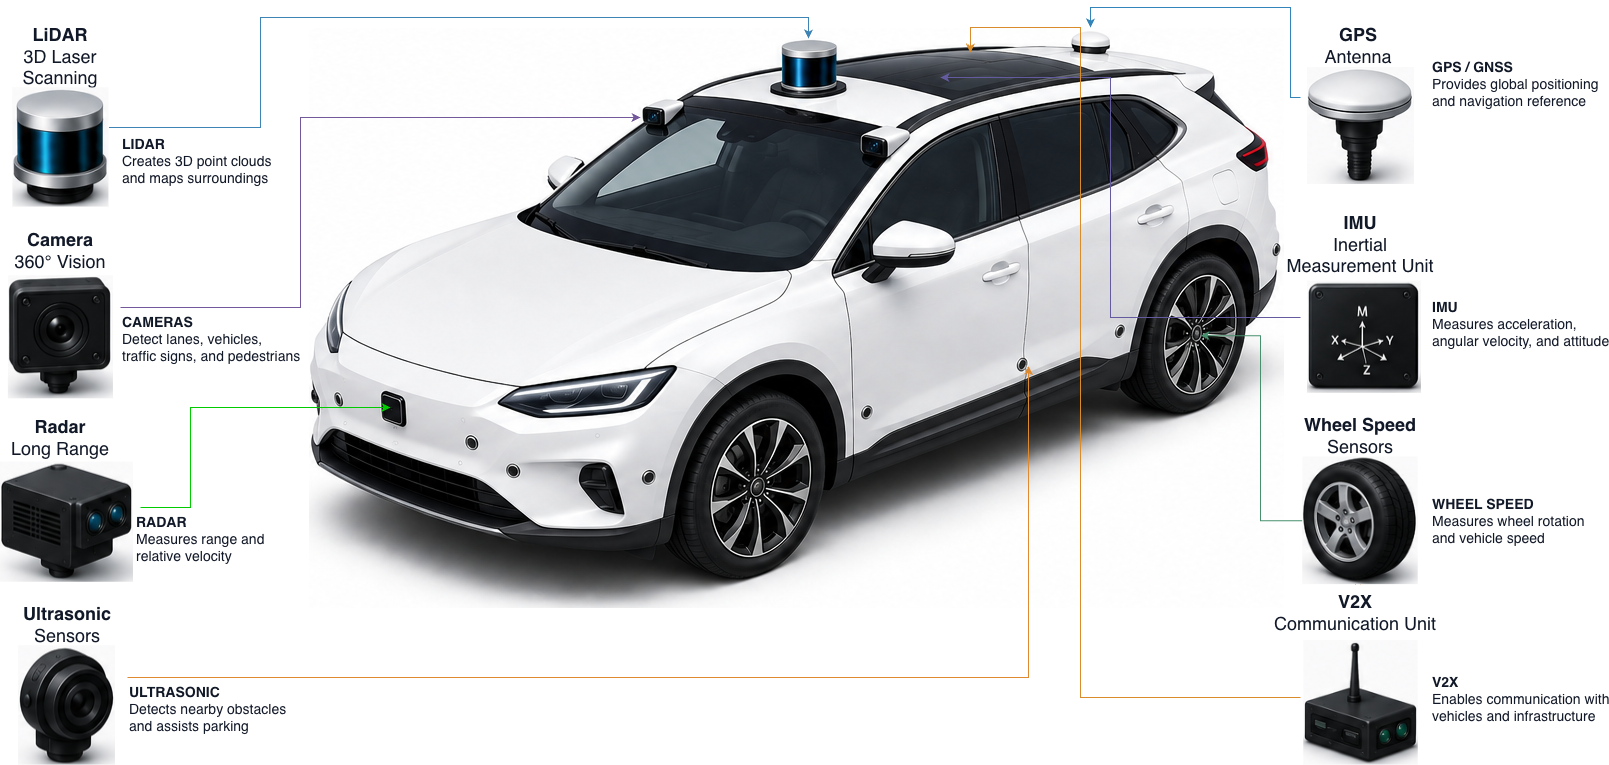
\includegraphics[width=\textwidth]{figures/autonomous_vehicle_sensors_layout_v02.png}
    \caption{Representative autonomous-vehicle sensor layout, showing complementary sensing modalities for perception, localisation, ego-motion estimation, short-range obstacle detection, and communication.}
    \label{fig:autonomous-vehicle-sensors-layout}
\end{figure}

The sensor layout in Fig.~\ref{fig:autonomous-vehicle-sensors-layout} highlights the complementarity that motivates autonomous-driving sensor fusion. The strengths, limitations, and typical fusion roles of the individual modalities are summarised in Tables~\ref{tab:av-onboard-sensors} and~\ref{tab:av-cooperative-inputs}; here we only note the overall pattern: cameras contribute semantics, LiDAR (light detection and ranging) contributes geometry, radar contributes range and velocity under poor visibility, ultrasonic sensors cover the near field, IMUs (inertial measurement units) and wheel odometry provide high-rate ego-motion subject to drift, and GNSS (global navigation satellite systems), maps, V2X (vehicle-to-everything) communication, and roadside infrastructure extend awareness beyond the onboard field of view.

These modalities are not interchangeable. Instead, each provides a different type of information, with different uncertainty, sampling rate, field of view, latency, and failure modes. Autonomous-driving fusion therefore aims to exploit both \emph{complementarity}, where one sensor provides information that another cannot, and \emph{redundancy}, where multiple sensors observe related aspects of the same scene and can be used for consistency checking, robustness, and fault tolerance.

Table~\ref{tab:av-onboard-sensors} summarises common onboard sensing modalities, while Table~\ref{tab:av-cooperative-inputs} summarises cooperative, localisation, and map-based inputs that support autonomous-driving fusion.

\begin{table}[!t]
    \centering
    \renewcommand{\arraystretch}{1.25}
    \small
    \caption{Onboard sensing modalities commonly used in autonomous-driving sensor fusion.}
    \label{tab:av-onboard-sensors}
    \begin{tabular}{p{0.08\linewidth} p{0.28\linewidth} p{0.30\linewidth} p{0.25\linewidth}}
        \hline
        \textbf{Sensor} & \textbf{Strengths} & \textbf{Limitations} & \textbf{Typical Fusion Role} \\
        \hline
        Camera & Dense appearance, colour, texture, lane markings, traffic signs, traffic lights, and semantic cues & Sensitive to lighting, glare, shadows, night-time conditions, adverse weather, and limited direct depth estimation & Semantic perception, object classification, lane detection, traffic-light recognition, image--LiDAR and image--radar fusion \\
        \hline
        LiDAR & Accurate 3D geometry, depth, object shape, road structure, and point-cloud representation & Higher cost, sparse at long range, affected by rain, fog, snow, and reflective surfaces & 3D object detection, mapping, localisation, free-space estimation, camera--LiDAR fusion \\
        \hline
        Radar & Long range, direct relative velocity, robustness to poor visibility and adverse weather & Lower angular resolution, multipath effects, ghost detections, noisier spatial structure & Object tracking, velocity estimation, long-range detection, radar--camera and radar--LiDAR fusion \\
        \hline
        \DIFdelbeginFL \DIFdelFL{Ultra-}\allowbreak\DIFdelFL{sonic }\DIFdelendFL \DIFaddbeginFL \DIFaddFL{Ultra-}\allowbreak \DIFaddFL{sonic }\DIFaddendFL & Low-cost short-range sensing, useful for parking and close obstacle detection & Very limited range, low spatial resolution, affected by surface geometry and environmental noise & Low-speed manoeuvring, parking assistance, near-field obstacle detection \\
        \hline
        IMU & High-rate acceleration and angular velocity, useful for short-term ego-motion estimation & Biases and integration drift accumulate over time & Ego-motion prediction, inertial navigation, GNSS--IMU, visual--inertial, and LiDAR--inertial fusion \\
        \hline
        Wheel odometry & Direct vehicle motion information, low cost, high update rate & Accumulates drift, affected by wheel slip, tyre deformation, and road surface conditions & Dead reckoning, vehicle state estimation, GNSS--IMU--odometry fusion \\
        \hline
    \end{tabular}
\end{table}

\begin{table}[!t]
    \centering
    \renewcommand{\arraystretch}{1.25}
    \small
    \caption{Cooperative sensing, localisation, and map-based inputs used in autonomous-driving fusion.}
    \label{tab:av-cooperative-inputs}
    \begin{tabular}{p{0.13\linewidth} p{0.26\linewidth} p{0.28\linewidth} p{0.24\linewidth}}
        \hline
        \textbf{Input} & \textbf{Strengths} & \textbf{Limitations} & \textbf{Typical Fusion Role} \\
        \hline
        GNSS & Provides global positioning in open-sky environments and supports absolute localisation & Degraded by tunnels, urban canyons, multipath, signal blockage, interference, and spoofing risks & Global localisation, correction of accumulated drift in GNSS--IMU, GNSS--wheel odometry, and map-based localisation \\
        \hline
        High-definition maps & Provide prior information about lanes, road boundaries, intersections, landmarks, traffic rules, and road topology & Can become outdated, require accurate localisation, and are costly to build, update, and maintain & Map matching, lane-level localisation, perception priors, planning context, road-structure reasoning \\
        \hline
        V2X communication & Extends perception beyond line of sight and can provide information from nearby vehicles, infrastructure, and traffic-management systems & Depends on connectivity, latency, standardisation, trust, cyber-security, and communication coverage & Cooperative perception, hazard warning, traffic-signal information, occlusion handling, extended situational awareness \\
        \hline
        Roadside infrastructure sensors & Provide external viewpoints from fixed cameras, LiDARs, radars, or smart-city infrastructure & Require deployment and maintenance, depend on communication links, and raise calibration, synchronisation, privacy, and security issues & Infrastructure-assisted perception, validation, cooperative tracking, scenario recording, ground-truth-like reference generation \\
        \hline
    \end{tabular}
\end{table}

\subsection{Indicative Sensor Characteristics}
\label{subsec:sensor-characteristics}

Tables~\ref{tab:av-onboard-sensors} and~\ref{tab:av-cooperative-inputs} are qualitative. Fusion design, however, needs numbers: the choice of filter rates, gating thresholds, process- and measurement-noise covariances and fallback strategies all depend on how fast, how far and how accurately each sensor observes the world. Table~\ref{tab:av-sensor-characteristics} therefore collects \emph{indicative orders of magnitude} for the sensors of Fig.~\ref{fig:autonomous-vehicle-sensors-layout}. The figures are representative of automotive-grade devices of the early 2020s and vary considerably with product, configuration and operating conditions \cite{yeong2021_sensors,patole2017_radar,groves2013_gnss}; they should be read as the starting point of a sensor-model identification, not as specifications.

\begin{table}[!t]
    \centering
    \renewcommand{\arraystretch}{1.25}
    \scriptsize
    \caption{Indicative characteristics of automotive sensors (orders of magnitude; actual values depend on the product, the configuration and the operating conditions). \DIFdelbeginFL \DIFdelFL{$1\sigma$ accuracies refer to a single measurement in }\DIFdelendFL \DIFaddbeginFL \DIFaddFL{The column mixes spatial resolution, }\DIFaddendFL nominal \DIFdelbeginFL \DIFdelFL{conditions}\DIFdelendFL \DIFaddbeginFL \DIFaddFL{accuracy ranges, and bias-stability specifications; the quoted $\pm$ limits are not uniformly $1\sigma$ values and must not be copied directly into $\mathbf{R}$}\DIFaddendFL . MEMS: micro-electro-mechanical systems; mg: $10^{-3}$ of the gravitational acceleration; RTK: real-time kinematic; PPP: precise point positioning; fixed/float: RTK solution with or without resolved carrier-phase ambiguities; ppm: millimetres per kilometre of distance from the reference station.}
    \label{tab:av-sensor-characteristics}
    \begin{tabular}{>{\raggedright\arraybackslash}p{0.15\linewidth} >{\raggedright\arraybackslash}p{0.10\linewidth} >{\raggedright\arraybackslash}p{0.13\linewidth} >{\raggedright\arraybackslash}p{0.24\linewidth} >{\raggedright\arraybackslash}p{0.28\linewidth}}
        \hline
        \textbf{Sensor} & \textbf{Update rate} & \textbf{Range} & \textbf{Resolution / accuracy} & \textbf{Main error sources} \\
        \hline
        Camera (mono, stereo, surround fisheye) & 10--60\,Hz & semantic: $>$200\,m; depth: 20--100\,m (stereo), poorer for mono & 1--8\,Mpx; angular resolution 0.02--0.1$^{\circ}$/pixel; mono range error 10--20\,\% of range & Illumination, glare, night, rain and fog, lens soiling, rolling shutter, calibration drift, depth ambiguity \\
        \hline
        Spinning or solid-state LiDAR & 10--20\,Hz & 100--250\,m (10\,\% reflectivity) & range $\pm$2--3\,cm; angular 0.1--0.4$^{\circ}$; 32--128 layers & Rain, fog and snow backscatter, blooming on retro-reflectors, motion distortion within a sweep, sparse returns at long range, dark or specular surfaces \\
        \hline
        77-GHz radar (long-range, corner, imaging) & 10--20\,Hz & 150--250\,m (long-range); 50--100\,m (corner) & range 0.1--0.5\,m; range rate $\pm$0.1\,m/s; azimuth 1--5$^{\circ}$ (0.1--1$^{\circ}$ imaging); poor elevation except for 4D imaging radar & Multipath and ghost targets, clutter, angular ambiguity, low resolution of extended objects, interference between radars \\
        \hline
        Ultrasonic & 10--40\,Hz & 0.2--5\,m & $\pm$1--3\,cm range, very coarse bearing & Temperature and wind, surface geometry and absorption, cross-talk, limited range \\
        \hline
        IMU, automotive MEMS grade & 100--1000\,Hz & -- & gyro bias instability 1--10$^{\circ}$/h, angle random walk 0.1--0.5$^{\circ}/\sqrt{\mathrm{h}}$; accelerometer bias 1--10\,mg & Bias (turn-on and in-run), scale factor, axis misalignment, temperature sensitivity, vibration; errors integrate into drift \\
        \hline
        IMU, tactical / navigation grade & 100--1000\,Hz & -- & bias instability 0.1--1$^{\circ}$/h (tactical), $<$0.01$^{\circ}$/h (navigation) & As above with smaller magnitude; cost, size and export restrictions limit automotive use \\
        \hline
        Wheel odometry & 50--100\,Hz & -- & speed $\pm$0.05--0.2\,m/s; scale error 1--2\,\% (tyre radius, pressure, load) & Slip and skid, surface, tyre deformation, quantisation at low speed, no direct heading \\
        \hline
        GNSS, single frequency & 1--10\,Hz & global & 2--5\,m horizontal (open sky) & Multipath, atmospheric delay, blockage in tunnels and urban canyons, interference and spoofing \\
        \hline
        GNSS, RTK / PPP-RTK & 1--20\,Hz & global & 1--3\,cm $+$ 1\,ppm (fixed solution); 0.1--1\,m (float) & Needs a correction link and visible satellites; ambiguity fixing lost in urban canyons; lever arm to the IMU must be calibrated \\
        \hline
    \end{tabular}
\end{table}

Two patterns in Table~\ref{tab:av-sensor-characteristics} recur throughout the rest of the chapter. First, exteroceptive sensors have \emph{angular} accuracies, so their Cartesian position errors grow linearly with range: a bearing error $\sigma_{\theta}$ at range $r$ produces a lateral error $\approx r\sigma_{\theta}$, which is $0.2$\,m at $60$\,m for a camera with $\sigma_{\theta}=0.2^{\circ}$ but $1.6$\,m for a radar with $\sigma_{\theta}=1.5^{\circ}$, while the radar range error stays at a few decimetres independently of $r$. This complementarity is exploited in Example~\ref{ex:camera-radar-ci}. Second, proprioceptive sensors have errors that \emph{integrate}: a gyroscope bias $b$ becomes a heading error $b\tau$ after a time $\tau$ and a cross-track position error of roughly $v b\tau^{2}/2$ at speed $v$. Such errors are small per sample but unbounded in time, which is why they must be corrected by an absolute reference and why bias states are included in the filter of Example~\ref{ex:gnss-imu-odom}.

\subsection{Sensor Placement, Field-of-View Coverage, and Redundancy}
\label{subsec:placement}

The placement of the sensors in Fig.~\ref{fig:autonomous-vehicle-sensors-layout} follows from their ranges and fields of view. A roof-mounted spinning LiDAR offers a $360^{\circ}$ horizontal field of view but leaves a near-field blind cone around the vehicle, which is covered by ultrasonic sensors, surround-view fisheye cameras and corner radars. Long-range radar and a forward camera (often a stereo pair or a multi-focal cluster) look along the driving direction, where the longest detection range and the best longitudinal accuracy are needed for adaptive cruise control and emergency braking, while corner radars cover the lateral sectors relevant to lane changes, cut-ins and intersections. The IMU is placed close to the centre of gravity to minimise lever-arm effects (the centripetal and tangential accelerations that an IMU mounted away from the centre of gravity senses when the vehicle rotates), and the GNSS antenna on the roof, so that its position must be related to the IMU by a lever arm $\mathbf{l}$, the fixed offset vector from the IMU to the antenna, expressed in the body frame: $\mathbf{p}_{\mathrm{GNSS}}=\mathbf{p}_{\mathrm{IMU}}+\mathbf{R}(\psi)\,\mathbf{l}$, where $\mathbf{R}(\psi)$ rotates body-frame vectors into the navigation frame, a relation that is itself part of the measurement model $\mathbf{g}(\cdot)$ of the localisation filter.

Coverage is designed so that every sector around the vehicle is observed by at least two modalities with different failure modes, which is the architectural expression of the redundancy discussed above. The overlap regions are also where cross-calibration is possible, because the same object or landmark is observed simultaneously by two sensors, and where consistency checks between modalities can detect a sensor that has drifted, been blocked or been soiled. The design therefore trades coverage, cost and computational load: more sensors improve redundancy but increase the alignment effort of Section~\ref{subsec:spatial-alignment}, the bandwidth of the data path and the number of calibrations that can silently degrade (Chapter~\ref{sec:open-challenges}).

\section{Fusion Pipeline and Architectural Levels}

Sensor fusion appears at several points in the autonomous-driving pipeline. A typical system includes sensing, calibration and synchronisation, preprocessing, perception, localisation and mapping, tracking, prediction, planning, and control. Measurements from cameras, LiDAR, radar, ultrasonic sensors, IMUs, wheel encoders, GNSS receivers, maps, V2X messages, and infrastructure sensors must first be temporally synchronised and spatially aligned. This usually requires intrinsic calibration, extrinsic calibration, timestamp correction, latency compensation, motion compensation, and coordinate-frame transformations. The mathematics of these alignment steps, and the consequences of performing them imperfectly, are developed in Sections~\ref{subsec:spatial-alignment}--\ref{subsec:calibration-errors}.

Figure~\ref{fig:autonomous-driving-fusion-pipeline} illustrates the main stages of a typical autonomous-driving sensor-fusion pipeline. The important point is that fusion is not confined to a single block. It can occur repeatedly at different abstraction levels and for different purposes.

\begin{figure}[!t]
    \centering
    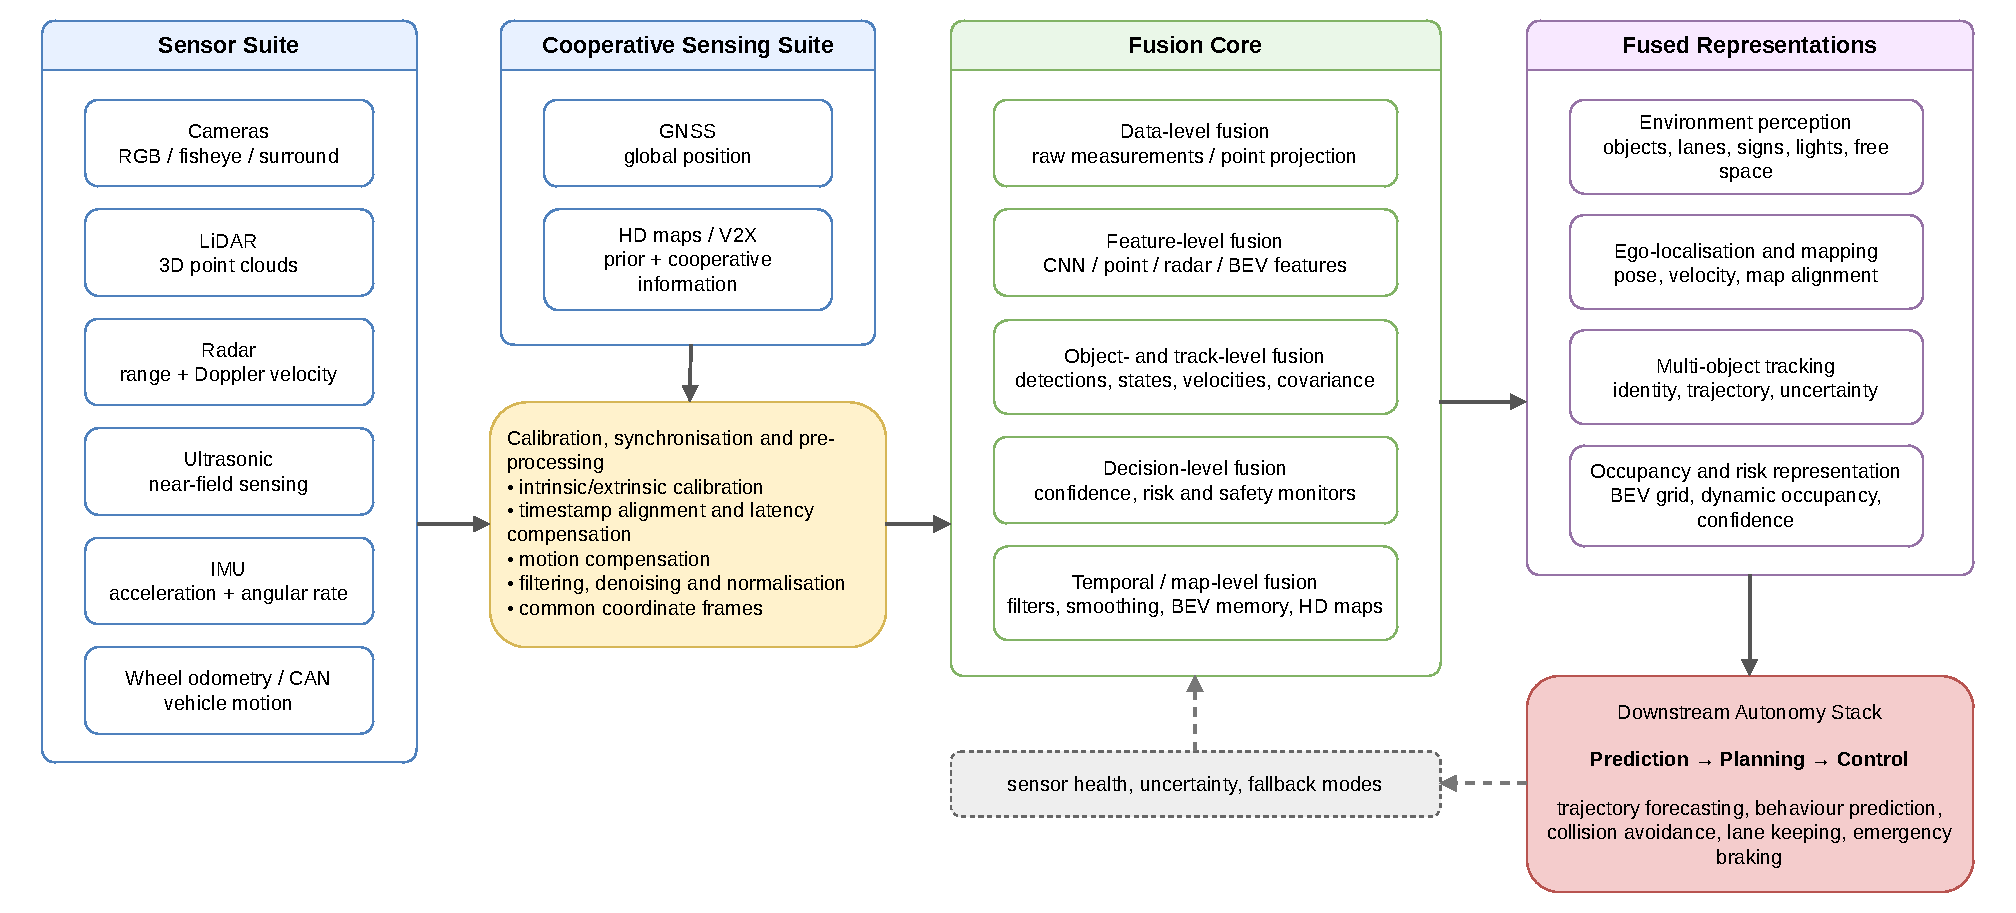
\includegraphics[width=\textwidth]{figures/autonomous_driving_fusion_pipeline.pdf}
    \caption{Autonomous-driving sensor fusion pipeline. Heterogeneous sensor measurements are calibrated, synchronised, and pre-processed before being fused at data, feature, object, decision, temporal, and map levels. The fused representations support environment perception, ego-localisation, mapping, tracking, occupancy estimation, prediction, planning, and control.}
    \label{fig:autonomous-driving-fusion-pipeline}
\end{figure}

Data-level fusion combines low-level measurements directly, for example by projecting LiDAR points into the image plane, aggregating multiple LiDAR sweeps, or associating radar detections with point-cloud clusters. Feature-level fusion combines extracted or learned representations, as in camera--LiDAR, camera--radar, LiDAR--radar, and bird's-eye-view (BEV) neural architectures, that is, the \emph{multimodal fusion} networks of Chapter~\ref{sec:learning}. Object- and track-level fusion combines detections, bounding boxes, velocities, class probabilities, covariances, and track states across sensors. Decision-level fusion combines classifier outputs, risk scores, occupancy decisions, or safety-monitoring signals. Temporal fusion uses filtering, smoothing, recurrent networks, temporal attention, or memory-based BEV representations to integrate information over time. Map-level fusion aligns online sensor observations with high-definition maps or previously built local maps.

This layered view clarifies why autonomous driving is a demanding fusion problem. The vehicle must combine onboard exteroceptive sensing for environment perception, proprioceptive sensing for ego-motion estimation, global and map-based references for localisation, and cooperative information for extended situational awareness \cite{2023:IEEE_ITSM,TANG2023109165}. These inputs must then be transformed into representations that are useful for downstream prediction, planning, and control. Errors in calibration, synchronisation, data association, uncertainty modelling, or sensor reliability estimation can therefore propagate through the entire autonomy stack.

\subsection{Spatial Alignment: Extrinsic Calibration and Projection}
\label{subsec:spatial-alignment}

All fusion operations presuppose that the measurements of different sensors are expressed in a common coordinate frame. Each sensor $S$ has its own frame, and the rigid-body pose of that frame with respect to the vehicle (body) frame $V$ is the \emph{extrinsic calibration}
\begin{equation}
\mathbf{T}_{V\!S}=
\begin{bmatrix}
\mathbf{R}_{V\!S} & \mathbf{t}_{V\!S}\\
\mathbf{0}^{\mathsf T} & 1
\end{bmatrix}\in SE(3),
\qquad
\mathbf{R}_{V\!S}\in SO(3),\ \mathbf{t}_{V\!S}\in\mathbb{R}^{3},
\label{eq:extrinsic-se3}
\end{equation}
which maps a point $\mathbf{p}^{S}$ measured in the sensor frame to $\mathbf{p}^{V}=\mathbf{R}_{V\!S}\mathbf{p}^{S}+\mathbf{t}_{V\!S}$, or, in homogeneous coordinates, $\tilde{\mathbf{p}}^{V}=\mathbf{T}_{V\!S}\tilde{\mathbf{p}}^{S}$ with $\tilde{\mathbf{p}}=[\mathbf{p}^{\mathsf T}\ 1]^{\mathsf T}$. Here $SO(3)$ is the group of 3D rotation matrices and $SE(3)$ the group of rigid-body transformations (a rotation followed by a translation); rotation matrices carry a subscript or an argument throughout the chapter, which distinguishes them from the measurement-noise covariance $\mathbf{R}$ of Table~\ref{tab:notation}. Transforms compose by matrix multiplication, so a LiDAR point is expressed in the camera frame through the vehicle frame as $\mathbf{T}_{C\!L}=\mathbf{T}_{V\!C}^{-1}\mathbf{T}_{V\!L}$, and in a world (map) frame $W$ through the ego pose as $\mathbf{T}_{W\!L}(t)=\mathbf{T}_{W\!V}(t)\,\mathbf{T}_{V\!L}$. The collection of such pairwise transforms, with the sensor frames attached to the vehicle frame and the vehicle frame attached to the world frame through the ego pose, is the \emph{transform tree} maintained by the middleware (Section~\ref{subsec:middleware}). Small rotation errors $\delta\boldsymbol{\theta}$ are conveniently written as $\widetilde{\mathbf{R}}_{V\!S}=\exp([\delta\boldsymbol{\theta}]_{\times})\,\mathbf{R}_{V\!S}\approx(\mathbf{I}+[\delta\boldsymbol{\theta}]_{\times})\mathbf{R}_{V\!S}$, with $\widetilde{\mathbf{R}}_{V\!S}$ the perturbed rotation, where $[\cdot]_{\times}$ is the skew-symmetric matrix of the cross product, which is the linearisation used both by calibration estimators and by the error analysis of Section~\ref{subsec:calibration-errors}; a self-contained treatment of $SE(3)$ for estimation is given in \cite{barfoot2017_state_estimation,sola2018_microlie}.

The camera adds an \emph{intrinsic} model. With the pinhole model and a point $\mathbf{p}^{C}=[X\ Y\ Z]^{\mathsf T}$ in the camera frame, the pixel coordinates $(u,v)$ satisfy
\begin{equation}
s\begin{bmatrix}u\\ v\\ 1\end{bmatrix}
=\mathbf{K}\,[\mathbf{R}_{C\!L}\ |\ \mathbf{t}_{C\!L}]\,\tilde{\mathbf{p}}^{L},
\qquad
\mathbf{K}=
\begin{bmatrix}
f_{x} & 0 & c_{x}\\
0 & f_{y} & c_{y}\\
0 & 0 & 1
\end{bmatrix},
\label{eq:lidar-to-image}
\end{equation}
with $s=Z$ the depth of the point, $f_{x},f_{y}$ the focal lengths in pixels and $(c_{x},c_{y})$ the principal point; lens distortion is applied to the normalised coordinates $(X/Z,Y/Z)$ before multiplication by $\mathbf{K}$ \cite{zhang2000_calibration}. Equation~\eqref{eq:lidar-to-image} is the operation behind data-level camera--LiDAR fusion: every LiDAR return with $Z>0$ that falls inside the image is given the colour, the semantic label or the learned feature of the pixel it projects to, and conversely image detections can be lifted to 3D by the LiDAR depth of the pixels they contain (Chapter~\ref{sec:learning}). The extrinsic parameters are estimated offline from a calibration target observed by both sensors \cite{geiger2012_calibration} and must be monitored online, because mounting brackets flex, temperature changes the optics and minor collisions move the sensors; such \emph{calibration drift} is among the open problems of Chapter~\ref{sec:open-challenges}.

\subsection{Temporal Alignment, Ego-Motion Compensation, and Delayed Measurements}
\label{subsec:temporal-alignment}

Sensors sample at different rates and instants, so a second alignment is needed in time. Every measurement carries a timestamp, ideally taken by hardware at the instant of exposure or of the laser pulse and expressed in a common clock (Section~\ref{subsec:middleware}). To relate a measurement taken at time $\tau$ to the ego pose, which is only available at the filter instants $t_{a}\le\tau\le t_{b}$, the pose is interpolated: the position linearly,
\begin{equation}
\mathbf{p}(\tau)=\mathbf{p}(t_{a})+\alpha\,[\mathbf{p}(t_{b})-\mathbf{p}(t_{a})],\qquad \alpha=\frac{\tau-t_{a}}{t_{b}-t_{a}},
\label{eq:pose-interp-pos}
\end{equation}
and the rotation along the geodesic of $SO(3)$,
\begin{equation}
\mathbf{R}(\tau)=\mathbf{R}(t_{a})\,\exp\!\big(\alpha\,\log(\mathbf{R}(t_{a})^{\mathsf T}\mathbf{R}(t_{b}))\big),
\label{eq:pose-interp-rot}
\end{equation}
where $\exp$ and $\log$ are the matrix exponential and logarithm of $SO(3)$ (equivalently, spherical linear interpolation of the corresponding quaternions). For typical vehicle dynamics the linear interpolation error is negligible for intervals of 10\,ms, whereas over the 100\,ms between two LiDAR sweeps it reaches about $1$\,cm in a turn at $25$\,m/s and $0.3$\,rad/s, comparable with the LiDAR range accuracy.

A rotating LiDAR does not measure a point cloud at one instant: the points of one sweep are acquired over the sweep period $T_{\mathrm{s}}$ (typically $100$\,ms at $10$\,Hz) while the vehicle moves. A point $\mathbf{p}_{i}^{L}$ acquired at time $t_{i}\in[t_{0},t_{0}+T_{\mathrm{s}}]$ is expressed in the vehicle frame at the sweep reference time $t_{0}$ by
\begin{equation}
\tilde{\mathbf{p}}_{i}^{V(t_{0})}=\mathbf{T}_{V(t_{0})V(t_{i})}\,\mathbf{T}_{V\!L}\,\tilde{\mathbf{p}}_{i}^{L},
\qquad
\mathbf{T}_{V(t_{0})V(t_{i})}=\mathbf{T}_{W\!V}(t_{0})^{-1}\mathbf{T}_{W\!V}(t_{i}),
\label{eq:motion-compensation}
\end{equation}
where the ego poses $\mathbf{T}_{W\!V}(t_{0})$ and $\mathbf{T}_{W\!V}(t_{i})$ are obtained by interpolating the high-rate IMU--odometry prediction of the localisation filter with \eqref{eq:pose-interp-pos}--\eqref{eq:pose-interp-rot}. Without this \emph{ego-motion compensation} (also called de-skewing or motion distortion correction), a vehicle travelling at $25$\,m/s displaces the first and the last point of the same sweep by $2.5$\,m, and a yaw rate of $0.3$\,rad/s rotates them by $1.7^{\circ}$, i.e. by $1.5$\,m laterally at $50$\,m range; the resulting distortions corrupt scan matching, object extents and the camera--LiDAR projection \eqref{eq:lidar-to-image} alike. LiDAR odometry methods such as LOAM (LiDAR odometry and mapping) and FAST-LIO2 perform this correction as part of the registration itself \cite{zhang2014_loam,xu2022_fastlio2}.

Latency produces a related problem at the level of the fusion filter. A camera detection that reaches the tracker $80$\,ms after exposure refers to the state at $t_{k}-80$\,ms, not at $t_{k}$: it is a \emph{delayed} or, if a more recent radar measurement has already been processed, an \emph{out-of-sequence} measurement (OOSM). Ignoring the delay biases the estimate by the motion during the delay, which at a relative speed of $30$\,m/s is $2.4$\,m. The exact treatment keeps a short buffer of past states, covariances and measurements, rolls the filter back to the measurement time $t_{m}$, applies the update there with the stored prediction $\widehat{\mathbf{x}}_{m|m-1}$ and $\mathbf{P}_{m|m-1}$, and re-propagates all later measurements; its cost is proportional to the number of buffered steps. An algebraic alternative retrodicts (predicts backwards in time) the current estimate to $t_{m}$ and updates it in a single step, exactly for a one-step lag and approximately for longer lags \cite{barshalom2002_oosm,barshalom2001_estimation}. In both cases the innovation, that is, the residual between the measurement and its prediction \eqref{eq:kf_innovation}, is formed against the state \emph{at the measurement time}, $\boldsymbol{\nu}=\mathbf{y}_{m}-\mathbf{g}(\widehat{\mathbf{x}}_{m|m-1})$ or $\boldsymbol{\nu}=\mathbf{y}_{m}-\mathbf{g}(\widehat{\mathbf{x}}_{m|k})$ respectively, and not against the current state; using the current state is a common timing error in practical trackers. Measurements older than a configured maximum lag are discarded.

\subsection{Effect of Calibration and Synchronisation Errors on Fusion}
\label{subsec:calibration-errors}

Alignment errors are systematic: they do not average out over time and they are not represented in the covariances $\mathbf{R}$ of the individual sensors, so they violate the zero-mean error model assumed by the probabilistic fusion rules of Chapter~\ref{sec:classicalSF}. Their effect can be quantified with the linearisation of \eqref{eq:extrinsic-se3}. A yaw (rotation about the vertical axis) error $\delta\psi$ in the extrinsic calibration of a sensor displaces a target at range $r$ laterally by
\begin{equation}
\Delta y \approx r\,\delta\psi,
\label{eq:yaw-error-lateral}
\end{equation}
so a $0.5^{\circ}$ error ($8.7$\,mrad) moves a target at $60$\,m by $0.52$\,m, i.e. by about $15$\,\% of a $3.5$\,m lane and by more than twice the lateral $1\sigma$ accuracy ($0.21$\,m) of the fused track in Example~\ref{ex:camera-radar-ci}, whereas at $10$\,m the same error produces only $0.09$\,m. In the image, the same yaw error shifts every projected LiDAR point by $\Delta u\approx f_{x}\,\delta\psi$, i.e. by $8.7$ pixels for $f_{x}=1000$\,pixels, independently of the range, which is why camera--LiDAR misalignment is visible as a constant offset at object boundaries. A translation error $\delta\mathbf{t}$, by contrast, adds a constant offset that does not grow with range, and is therefore less harmful for distant objects but critical for near-field manoeuvring. A time offset $\delta t$ between two sensors is equivalent to a position error $\mathbf{v}_{\mathrm{rel}}\,\delta t$ along the relative velocity: $20$\,ms at $25$\,m/s is $0.5$\,m for a static obstacle and $1.0$\,m for an oncoming vehicle at the same speed.

The consequences for fusion are threefold. Associations fail: a lateral offset of $0.5$\,m against a lateral innovation standard deviation of $0.2$\,m gives a normalised distance of $2.5\sigma$ ($d^{2}=6.25$, beyond the $95$\,\% gate $\gamma=5.99$ for two degrees of freedom), so the association gate \eqref{eq:mahalanobis_gate} starts rejecting correct associations and duplicate tracks appear. Estimates become biased and the filter inconsistent, that is, its actual errors exceed what its reported covariance allows: the normalised innovation squared (NIS) \eqref{eq:nis} grows persistently rather than transiently, which \DIFdelbegin \DIFdel{is the signature that distinguishes a }\DIFdelend \DIFaddbegin \DIFadd{can suggest a persistent fault but does not uniquely distinguish }\DIFaddend calibration error from \DIFdelbegin \DIFdel{the model mismatchof Example~\ref{ex:ekf-radar-cutin}}\DIFdelend \DIFaddbegin \DIFadd{persistent process-model mismatch}\DIFaddend . Finally, errors that are common to two sensors, for instance the ego-pose used to express both in the map frame, are \emph{correlated} and are double-counted by independent fusion; Example~\ref{ex:camera-radar-ci} quantifies this effect and shows how covariance intersection protects against it. The practical response is to monitor alignment online, by cross-modal consistency statistics and by estimating small calibration corrections as slowly varying states, in the same way as the sensor biases of Example~\ref{ex:gnss-imu-odom}.

\section{Core Fusion Tasks}

Autonomous-driving fusion supports several core tasks. The first is environment perception, where cameras, LiDAR, radar, and maps are used to estimate drivable space, lanes, road boundaries, traffic signs, traffic lights, vehicles, cyclists, pedestrians, and other obstacles. LiDAR depth can improve the spatial accuracy of image-based segmentation, while image semantics can improve the interpretation of sparse point clouds. Radar can contribute long-range range-rate information, especially for moving objects and adverse-weather scenarios. Map priors can further help distinguish valid road areas, pavements, junctions, and lane-level structure.

A second major task is three-dimensional object detection and tracking. Camera--LiDAR fusion is widely used for accurate 3D bounding-box estimation and classification~\cite{bai2022_transfusion,liu2023_bevfusion}, while radar is valuable for long-range detection and velocity estimation~\cite{nabati2021_centerfusion,kim2023_crn}. Tracking extends detection over time by maintaining object identity, position, velocity, acceleration, heading, and uncertainty. Classical filters, smoothing methods, data-association algorithms, and track-management logic remain important even when the detections themselves are produced by deep neural networks.

A third task is ego-localisation and mapping. GNSS, IMU, wheel odometry, cameras, LiDAR, and high-definition maps are fused to estimate the vehicle's position and orientation relative to a local map, global frame, or lane-level map. GNSS alone is insufficient in tunnels, dense urban areas, and multipath environments, while inertial and odometry estimates drift over time. Visual, LiDAR, and map-based localisation can correct this drift, but must handle outdated maps, temporary roadworks, changed lane layouts, perceptual aliasing, and localisation uncertainty.

A fourth task is occupancy, free-space, and risk estimation. Instead of representing the scene only as a list of detected objects, occupancy-based fusion (Chapter~\ref{sec:learning}) estimates which regions of space are free, occupied, unknown, or dynamically occupied. Risk-aware fusion can incorporate object uncertainty, time-to-collision, occlusion regions, road boundaries, predicted future occupancy, and traffic-rule constraints. These representations are especially important for prediction and planning because the planner must act not only on what is detected, but also on what may be hidden, uncertain, or about to enter the vehicle's path.

Robustness is central to all of these tasks. Rain, fog, snow, darkness, glare, dust, road spray, sensor contamination, and unusual traffic behaviour affect modalities differently. Reliability-aware fusion can adjust sensor weights according to environmental conditions and sensor-health indicators, while temporal fusion can reduce transient false positives and improve consistency. However, fusion cannot compensate for all failures. If several modalities degrade simultaneously, or if the scene lies outside the training or design distribution, the fusion system must detect its own uncertainty and support conservative fallback behaviour.

The remainder of this section makes two of these tasks concrete with runnable worked examples in the style of Chapter~\ref{sec:classicalSF}: ego-localisation by GNSS--IMU--wheel-odometry fusion (Example~\ref{ex:gnss-imu-odom}) and object-level camera--radar track fusion (Example~\ref{ex:camera-radar-ci}). Both use the notation of Table~\ref{tab:notation}; the scripts that generate every number and figure are in the companion repository under \repopath{companion\_\allowbreak repo/\allowbreak examples/\allowbreak }, in the folders \repopath{ch05\_\allowbreak gnss\_\allowbreak imu\_\allowbreak odometry\_\allowbreak ekf} and \repopath{ch05\_\allowbreak camera\_\allowbreak radar\_\allowbreak ci\_\allowbreak fusion}.

\subsection{Worked Example: Ego-Localisation by GNSS--IMU--Wheel-Odometry Fusion}
\label{subsec:ex-gnss}

\begin{example}[GNSS--IMU--wheel-odometry fusion through a tunnel]
\label{ex:gnss-imu-odom}
Consider a vehicle driving for $120$\,s at $13$--$15$\,m/s along a route with a long left curve (yaw rate $0.08$\,rad/s between $t=15$ and $35$\,s) and a right curve ($-0.06$\,rad/s between $t=55$ and $70$\,s). A single-frequency GNSS receiver provides horizontal position fixes at $2$\,Hz with a standard deviation of $\sigma_{\mathrm{GNSS}}=1.5$\,m per axis, except between $t=50$ and $75$\,s, when the vehicle crosses a $346$\,m tunnel and no fix is available. A MEMS gyroscope measures the yaw rate at $100$\,Hz with white noise of standard deviation $0.002$\,rad/s per sample and a constant bias $b=10$\,mrad/s ($0.57^{\circ}$/s), an uncalibrated turn-on offset typical of a low-cost MEMS part (the bias instability of Table~\ref{tab:av-sensor-characteristics} describes instead the much smaller in-run variation that remains once such an offset has been estimated), and the wheel encoders provide the speed at $100$\,Hz with noise $0.05$\,m/s and a scale error $s=+2$\,\% caused by an incorrect tyre radius. The planar unicycle state
\begin{equation}
\mathbf{x}_{k}=
\begin{bmatrix}
p_{x,k} & p_{y,k} & \psi_{k} & b_{k} & s_{k}
\end{bmatrix}^{\mathsf T}
\end{equation}
collects the position in a local east--north frame, the heading, the gyroscope bias and the wheel scale error. The measured inputs $\mathbf{u}_{k}=[v_{m,k}\ \ \omega_{m,k}]^{\mathsf T}$ drive the process model $\mathbf{f}(\cdot)$ of \eqref{eq:bayes_process_model},
\begin{equation}
\begin{aligned}
p_{x,k+1}&=p_{x,k}+T\,\hat v_{k}\cos\psi_{k}, &\qquad \hat v_{k}&=\frac{v_{m,k}}{1+s_{k}},\\
p_{y,k+1}&=p_{y,k}+T\,\hat v_{k}\sin\psi_{k}, &\qquad \psi_{k+1}&=\psi_{k}+T\,(\omega_{m,k}-b_{k}),\\
b_{k+1}&=b_{k}+q_{b,k}, &\qquad s_{k+1}&=s_{k}+q_{s,k},
\end{aligned}
\label{eq:gnss-imu-process}
\end{equation}
with $T=0.01$\,s. The bias and the scale error are modelled as random walks with intensities $10^{-4}$\,rad\,s$^{-1}$/$\sqrt{\mathrm{s}}$ and $10^{-4}/\sqrt{\mathrm{s}}$, and the input noise enters the position and heading through the Jacobian of \eqref{eq:gnss-imu-process} with respect to $\mathbf{u}_{k}$, denoted $\mathbf{G}_{k}$ here and not to be confused with the measurement matrix $\mathbf{G}$ of Table~\ref{tab:notation}, so that $\mathbf{Q}_{k}=\mathbf{G}_{k}\mathbf{W}\mathbf{G}_{k}^{\mathsf T}+\diag(0,0,T\sigma_{\psi}^{2},T\sigma_{b}^{2},T\sigma_{s}^{2})$ with $\mathbf{W}=\diag(0.05^{2},0.002^{2})$. The GNSS measurement model is linear, $\mathbf{y}_{k}=\mathbf{G}\mathbf{x}_{k}+\mathbf{r}_{k}$ with $\mathbf{G}=[\mathbf{I}_{2}\ \ \mathbf{0}_{2\times3}]$ and $\mathbf{R}=\sigma_{\mathrm{GNSS}}^{2}\mathbf{I}_{2}$, and the extended Kalman filter (EKF) of Chapter~\ref{sec:classicalSF}, \eqref{eq:kf_state_prediction}--\eqref{eq:kf_cov_update} with the Jacobian $\mathbf{F}_{k}=\partial\mathbf{f}/\partial\mathbf{x}$ and $\mathbf{H}_{k}=\mathbf{G}$, is run at the IMU rate with a GNSS update every $50$ steps. The filter is initialised at the first fix with a $2^{\circ}$ heading error, $b_{0}=s_{0}=0$ and $\mathbf{P}_{0}=\diag(1.5^{2},1.5^{2},(5^{\circ})^{2},0.02^{2},0.05^{2})$. For comparison, a three-state filter $[p_{x}\ p_{y}\ \psi]$ that ignores the bias and the scale error is run on the same data; its heading process noise is inflated ($5\times10^{-3}$\,rad/$\sqrt{\mathrm{s}}$ against $10^{-3}$) so that it works acceptably while GNSS is available.

Figure~\ref{fig:gnss-imu-odom} summarises the outcome. While GNSS fixes are available, both filters follow the route, the five-state filter with a root-mean-square (RMS) position error of $0.60$\,m, well below the $2.1$\,m RMS horizontal error of a single fix ($1.5$\,m per axis), and the three-state filter with $5.02$\,m, because the uncompensated bias continuously pulls the heading away and GNSS can only correct it slowly. In the $50$\,s before the tunnel the five-state filter has also \emph{identified} the sensor errors: at the tunnel entrance it estimates $b=10.29\pm1.39$\,mrad/s ($3\sigma$) against a true value of $10.00$\,mrad/s, and $s=2.15\pm0.33$\,\% against $2.00$\,\%. These two states are observable, that is, they can be inferred from the measurement sequence, only because the GNSS fixes constrain the integrated effect of the biases on position: a bias is distinguishable from a true turn only when the position measurements reveal that the heading did not change as the gyroscope claimed. This happens on straight and curved stretches alike: the $3\sigma$ bound on $b$ falls from $60$ to about $3$\,mrad/s within the first $20$\,s (panel~c).

Inside the tunnel the filter dead-reckons on the compensated sensors, integrating speed and yaw rate without any position correction. The five-state position error grows to $3.56$\,m at the end of the $25$\,s outage, while the $3\sigma$ radius $3\sqrt{P_{xx}+P_{yy}}$ reported by the filter grows to $11.94$\,m: the error stays inside the bound throughout the run ($100$\,\% of the samples), \DIFdelbegin \DIFdel{so the estimate remains }\emph{\DIFdel{consistent}} %DIFAUXCMD
\DIFdel{and downstream modules can trust the covariance they receive. The }\DIFdelend \DIFaddbegin \DIFadd{which is encouraging for this realisation but does not prove a covariance bound. The radius $3\sqrt{\tr P}$ is a circular trace-based diagnostic, not a $99.73\,\%$ two-dimensional confidence ellipse. The }\DIFaddend three-state filter instead drifts to $63.88$\,m with a heading error of $17.3^{\circ}$, and reports a $3\sigma$ radius of only $19.83$\,m; its error lies inside its own bound for only $7.0$\,\% of the samples. Both filters process the same data; the difference is that the three-state filter has no state in which to put the systematic error, so the error accumulates as $vb\tau^{2}/2$ and the covariance, which only knows about white noise, cannot account for it. At re-acquisition the five-state filter converges within $0.52$\,m after $2$\,s and $0.10$\,m after $5$\,s, whereas the three-state filter still shows $8.79$\,m and $4.45$\,m, because a large heading error must be corrected through position fixes before the position itself can be trusted. \DIFdelbegin \DIFdel{The consistency of the five-state filter is confirmed }\DIFdelend \DIFaddbegin \DIFadd{Additional evidence from this run is provided }\DIFaddend by the NIS \eqref{eq:nis} of the GNSS updates, whose mean over the run is $1.80$ against an expected value of $2$, with $95.2$\,\% of the samples inside the two-sided $95$\,\% interval of $\chi^{2}_{2}$.

This applies to every proprioceptive sensor of Table~\ref{tab:av-sensor-characteristics}: what bounds the drift during an outage is not the quality of the IMU alone but the extent to which its systematic errors have been estimated \emph{before} the outage, and the covariance reported during the outage is only credible if those errors are states of the filter. In practice, longer outages are bridged by adding map matching, visual or LiDAR odometry as further corrections, which is the multi-sensor localisation problem of Chapter~\ref{sec:learning}, and without such aid the drift accumulated inside the tunnel in this example exceeds $0.5$\,m, the order of a lane-level accuracy requirement, after about $6$\,s.
\end{example}

\begin{figure}[!t]
\centering
\resizebox{0.99\columnwidth}{!}{
\begin{tikzpicture}
\begin{groupplot}[
    group style={group size=1 by 3, vertical sep=22mm},
    width=0.95\columnwidth,
    scale only axis,
    tick label style={font=\scriptsize},
    label style={font=\scriptsize},
    legend style={font=\scriptsize, draw=none, fill=white, fill opacity=0.85,
                  text opacity=1},
    grid=major,
    grid style={line width=0.2pt, draw=gray!25},
    axis line style={line width=0.5pt},
    tick align=outside,
    title style={font=\scriptsize, yshift=0.5mm},
]

\nextgroupplot[
    height=3.4cm,
    xlabel={east [m]},
    ylabel={north [m]},
    xmin=-50, xmax=1050,
    ymin=-50, ymax=1150,
    legend pos=north west,
    legend cell align=left,
    legend columns=2,
    title={(a) route in the local east--north frame},
    unbounded coords=discard,
]
\addplot[only marks, mark=*, mark size=0.5pt, draw=MeasGrey, fill=MeasGrey]
    table[x=px_gnss, y=py_gnss, col sep=comma] {data/ch05/gnss_imu_odometry.csv};
\addlegendentry{GNSS fixes}
\addplot[TruthBlack, line width=1.0pt]
    table[x=px_true, y=py_true, col sep=comma] {data/ch05/gnss_imu_odometry.csv};
\addlegendentry{ground truth}
\addplot[EkfBlue, line width=0.9pt, densely dashed]
    table[x=px_est, y=py_est, col sep=comma] {data/ch05/gnss_imu_odometry.csv};
\addlegendentry{EKF, bias states}
\addplot[ManoeuvreOrange!80!black, line width=0.9pt, densely dotted]
    table[x=px_est3, y=py_est3, col sep=comma] {data/ch05/gnss_imu_odometry.csv};
\addlegendentry{EKF, no bias states}
\node[anchor=west, font=\scriptsize, text=black!60] at (axis cs:520,530) {tunnel ($50$--$75$\,s)};
\draw[->, >=stealth, gray!70, line width=0.5pt] (axis cs:515,530) -- (axis cs:455,530);


\nextgroupplot[
    height=2.9cm,
    xlabel={time $t$ [s]},
    ylabel={position error [m]},
    xmin=0, xmax=120,
    ymin=0, ymax=70,
    ytick={0,20,40,60},
    legend pos=north west,
    legend cell align=left,
    legend columns=2,
    title={(b) position error and reported $3\sigma$ radius},
]
\addplot[draw=none, fill=ManoeuvreOrange, fill opacity=0.45, forget plot]
    coordinates {(50,0) (75,0) (75,70) (50,70)} \closedcycle;
\addplot[draw=none, fill=BandGrey, forget plot]
    table[x=t, y=rad3sig, col sep=comma] {data/ch05/gnss_imu_odometry.csv} \closedcycle;
\addplot[EkfBlue, line width=0.8pt]
    table[x=t, y=err, col sep=comma] {data/ch05/gnss_imu_odometry.csv};
\addlegendentry{error, bias states}
\addplot[RevisionRed!70!black, line width=0.8pt, densely dashed]
    table[x=t, y=err_nobias, col sep=comma] {data/ch05/gnss_imu_odometry.csv};
\addlegendentry{error, no bias states}
\addplot[gray!60, line width=0.5pt, densely dotted]
    table[x=t, y=rad3sig_nobias, col sep=comma] {data/ch05/gnss_imu_odometry.csv};
\addlegendentry{$3\sigma$ radius, no bias states}
\node[anchor=south, font=\scriptsize, text=black!70] at (axis cs:62.5,28) {GNSS outage};
\node[anchor=west, font=\scriptsize, text=black!55] at (axis cs:76,14) {$3\sigma$ radius, bias states (grey band)};


\nextgroupplot[
    height=2.6cm,
    xlabel={time $t$ [s]},
    ylabel={gyro bias $b$ [mrad/s]},
    xmin=0, xmax=120,
    ymin=0, ymax=20,
    ytick={0,5,10,15,20},
    title={(c) gyroscope-bias estimate with $3\sigma$ band (true value $10$\,mrad/s)},
]
\addplot[draw=none, fill=ManoeuvreOrange, fill opacity=0.45, forget plot]
    coordinates {(50,0) (75,0) (75,20) (50,20)} \closedcycle;
\addplot[name path=bu, draw=none, forget plot]
    table[x=t, y expr=\thisrow{b_est_mrad}+\thisrow{b_sig3_mrad}, col sep=comma] {data/ch05/gnss_imu_odometry.csv};
\addplot[name path=bl, draw=none, forget plot]
    table[x=t, y expr=\thisrow{b_est_mrad}-\thisrow{b_sig3_mrad}, col sep=comma] {data/ch05/gnss_imu_odometry.csv};
\addplot[BandGrey, forget plot] fill between[of=bu and bl];
\addplot[draw=gray!70, line width=0.5pt, densely dotted, forget plot]
    coordinates {(0,10) (120,10)};
\addplot[EkfBlue, line width=0.8pt]
    table[x=t, y=b_est_mrad, col sep=comma] {data/ch05/gnss_imu_odometry.csv};
\end{groupplot}
\end{tikzpicture}
}
\caption{GNSS--IMU--wheel-odometry fusion through a $25$\,s GNSS outage (Example~\ref{ex:gnss-imu-odom}). (a)~Route, GNSS fixes and the estimates of the five-state EKF with gyroscope-bias and wheel-scale states and of the three-state EKF without them. (b)~Position error of the two filters, the $3\sigma$ radius $3\sqrt{P_{xx}+P_{yy}}$ reported by each, and the outage (shaded). The five-state error stays inside its bound and recovers within a few fixes; the three-state error leaves its bound almost immediately because the covariance has no term for the uncompensated bias. (c)~The bias estimate converges within the first $20$\,s, as the GNSS fixes reveal that the heading did not change as the gyroscope claimed, and is frozen (with slowly growing uncertainty) during the outage.}
\label{fig:gnss-imu-odom}
\end{figure}

\subsection{Worked Example: Object-Level Camera--Radar Track Fusion}
\label{subsec:ex-camradar}

\begin{example}[Camera--radar track fusion with and without covariance intersection]
\label{ex:camera-radar-ci}
A camera track and a radar track refer to the same vehicle at range $r=60$\,m and bearing $\theta=10^{\circ}$ to the left, i.e. at $\mathbf{x}=[59.09\ \ 10.42]^{\mathsf T}$\,m in the ego frame of Example~\ref{ex:ekf-radar-cutin} ($x$ forward, $y$ to the left). The monocular camera estimates the bearing with $\sigma_{\theta}=0.2^{\circ}$ but the range only with $\sigma_{r}=15$\,\% of $r$, i.e. $9$\,m; the radar estimates the range with $\sigma_{r}=0.25$\,m but the bearing with $\sigma_{\theta}=1.5^{\circ}$ (Table~\ref{tab:av-sensor-characteristics}). Each local tracker reports its estimate in Cartesian coordinates with the covariance obtained by linearising the polar-to-Cartesian map, $\mathbf{P}_{i}=\mathbf{J}\,\diag(\sigma_{r,i}^{2},\sigma_{\theta,i}^{2})\,\mathbf{J}^{\mathsf T}$ with $\mathbf{J}=\partial(x,y)/\partial(r,\theta)$, the inverse of the position block of the radar Jacobian \eqref{eq:ekf-radar-jacobian}. The resulting standard deviations are listed in Table~\ref{tab:camera-radar-ci}: the camera ellipse is long and thin along the line of sight (semi-axes $9.00$ and $0.21$\,m), the radar ellipse is short and wide across it ($1.57$ and $0.25$\,m), so each sensor is informative exactly where the other is not.

If the two track errors are independent, the information-additive rule \eqref{eq:independent-track-fusion-state} applies and the fused covariance is $\mathbf{P}_{\mathrm{f}}=(\mathbf{P}_{1}^{-1}+\mathbf{P}_{2}^{-1})^{-1}$, with standard deviations of $0.25$\,m longitudinally and $0.21$\,m laterally: the fusion keeps the radar range and the camera bearing, and the trace of the covariance drops from $2.53$\,m$^{2}$ (radar alone) to $0.106$\,m$^{2}$. Covariance intersection (CI) \eqref{eq:ci-cov}--\eqref{eq:ci-est} with the trace criterion \eqref{eq:ci-weight} selects $\omega^{\star}=0.449$ (the weight of the camera track) and returns $0.34$\,m and $0.31$\,m, a trace of $0.209$\,m$^{2}$: CI pays about a factor of two in variance for not assuming independence, but it still combines the two sensors directionally, because the scalar $\omega$ weights whole information matrices $\mathbf{P}_{i}^{-1}$ and the camera information is concentrated in the bearing direction, in which the radar has little.

\begin{table}[!t]
    \centering
    \small
    \caption{Reported standard deviations of the local and fused tracks of Example~\ref{ex:camera-radar-ci} (independent-error case): longitudinal $\sigma_{x}$, lateral $\sigma_{y}$, semi-axes of the $1\sigma$ ellipse, and trace of the covariance.}
    \label{tab:camera-radar-ci}
    \begin{tabular}{lcccccc}
        \hline
        \textbf{Track} & $\sigma_{x}$ [m] & $\sigma_{y}$ [m] & major [m] & minor [m] & $\tr\mathbf{P}$ [m$^{2}$] & $\omega$ \\
        \hline
        Camera & 8.86 & 1.58 & 9.00 & 0.21 & 81.04 & -- \\
        Radar & 0.37 & 1.55 & 1.57 & 0.25 & 2.53 & -- \\
        Naive independent fusion & 0.25 & 0.21 & 0.25 & 0.21 & 0.106 & -- \\
        Covariance intersection & 0.34 & 0.31 & 0.34 & 0.31 & 0.209 & 0.449 \\
        \hline
    \end{tabular}
\end{table}

The loss is worth accepting because in a real vehicle the two tracks are not independent. Both are expressed in the same frame with the same ego-heading estimate, both may have been initialised from a common detection, both may share the map prior or the ego-motion compensation of Section~\ref{subsec:temporal-alignment}. Suppose the ego heading used by both trackers has an error $\delta\psi$ with standard deviation $\sigma_{\psi}$. It displaces both estimates by the same vector $\delta\psi\,\mathbf{u}$ with $\mathbf{u}=[-p_{y}\ \ p_{x}]^{\mathsf T}$, so that each local covariance becomes $\mathbf{P}_{i}+\sigma_{\psi}^{2}\mathbf{u}\mathbf{u}^{\mathsf T}$ and the cross-covariance is $\mathbf{P}_{12}=\sigma_{\psi}^{2}\mathbf{u}\mathbf{u}^{\mathsf T}$. The actual error covariance of any linear fusion $\widehat{\mathbf{x}}_{\mathrm{f}}=\mathbf{W}_{1}\widehat{\mathbf{x}}_{1}+\mathbf{W}_{2}\widehat{\mathbf{x}}_{2}$ with $\mathbf{W}_{1}+\mathbf{W}_{2}=\mathbf{I}$ is $\mathbf{W}_{1}\mathbf{P}_{1}\mathbf{W}_{1}^{\mathsf T}+\mathbf{W}_{2}\mathbf{P}_{2}\mathbf{W}_{2}^{\mathsf T}+\mathbf{W}_{1}\mathbf{P}_{12}\mathbf{W}_{2}^{\mathsf T}+\mathbf{W}_{2}\mathbf{P}_{12}^{\mathsf T}\mathbf{W}_{1}^{\mathsf T}$, where $\mathbf{P}_{1}$ and $\mathbf{P}_{2}$ now include the shared term, and its consistency can be measured by the expected normalised estimation error squared, $\mathrm{NEES}=\tr(\mathbf{P}_{\mathrm{rep}}^{-1}\mathbf{P}_{\mathrm{act}})$, which equals the state dimension $2$ \DIFdelbegin \DIFdel{for an exactly consistent filter and exceeds it for an over-confident one }\DIFdelend \DIFaddbegin \DIFadd{when the reported covariance equals the true zero-mean error covariance. A value at most $2$ is necessary for a covariance upper bound, but is not sufficient: excess uncertainty in one direction can hide under-reporting in another. Bias adds $\mathbf{b}^{\mathsf T}\mathbf{P}_{\mathrm{rep}}^{-1}\mathbf{b}$ to the expectation }\DIFaddend (Section~\ref{subsec:metrics}). Figure~\ref{fig:camera-radar-ci}(c) sweeps $\sigma_{\psi}$ from $0$ to $2^{\circ}$. The naive rule is consistent only at $\sigma_{\psi}=0$; at $\sigma_{\psi}=0.5^{\circ}$, the calibration-error magnitude of Section~\ref{subsec:calibration-errors}, its NEES is $2.18$ and the actual lateral standard deviation is $0.57$\,m against a reported $0.53$\,m; at $1^{\circ}$ the NEES is $2.47$ ($1.11$\,m actual against $0.92$\,m reported) and at $2^{\circ}$ it is $2.78$ ($2.15$\,m against $1.62$\,m). CI adapts its weight ($\omega^{\star}=0.667$ at $0.5^{\circ}$, $0.814$ at $2^{\circ}$) and remains consistent throughout, with a NEES between $1.00$ and $1.13$ and a reported lateral standard deviation that is never smaller than the actual one ($0.67$\,m reported against $0.56$\,m actual at $0.5^{\circ}$). A Monte-Carlo check with $20\,000$ trials at $\sigma_{\psi}=0.5^{\circ}$ reproduces the analytic values ($2.17$ for the naive rule and $1.04$ for CI), and shows that the two fused estimates are in fact almost equally accurate (RMS lateral errors $0.57$ and $0.56$\,m): what differs is the reported covariance, which the naive rule understates ($0.53$ against $0.57$\,m) and CI overstates ($0.67$ against $0.56$\,m).

The example thus answers the question of when CI is needed. If the fusion centre knows that the two tracks have never shared information, the independent rule is optimal and CI is needlessly conservative (here it doubles the trace of the fused covariance). If the tracks share a prior, a process-noise realisation, an ego pose or a calibration, and the cross-covariance is not tracked, the independent rule under-reports its uncertainty by a factor that grows with the shared component, which in turn corrupts the gates \eqref{eq:mahalanobis_gate} of later associations and the risk estimates of the planner. CI, or its known-correlation counterpart \eqref{eq:correlated-track-fusion-state} when $\mathbf{P}_{12}$ can be propagated, is then the appropriate rule, and it is the standard choice when tracks come from independently developed modules, from other vehicles or from roadside units (Chapter~\ref{sec:MAS}).
\end{example}

\begin{figure}[!t]
\centering
\DIFdelbeginFL %DIFDELCMD < \resizebox{0.99\columnwidth}{!}{
%DIFDELCMD < \begin{tikzpicture}
%DIFDELCMD < \begin{groupplot}[
%DIFDELCMD <     group style={group size=1 by 3, vertical sep=20mm},
%DIFDELCMD <     width=0.95\columnwidth,
%DIFDELCMD <     scale only axis,
%DIFDELCMD <     tick label style={font=\scriptsize},
%DIFDELCMD <     label style={font=\scriptsize},
%DIFDELCMD <     legend style={font=\scriptsize, draw=none, fill=white, fill opacity=0.85,
%DIFDELCMD <                   text opacity=1},
%DIFDELCMD <     grid=major,
%DIFDELCMD <     grid style={line width=0.2pt, draw=gray!25},
%DIFDELCMD <     axis line style={line width=0.5pt},
%DIFDELCMD <     tick align=outside,
%DIFDELCMD <     title style={font=\scriptsize, yshift=0.5mm},
%DIFDELCMD < ]
%DIFDELCMD < 

%DIFDELCMD < \nextgroupplot[
%DIFDELCMD <     height=2.6cm,
%DIFDELCMD <     xlabel={longitudinal $p_x$ [m]},
%DIFDELCMD <     ylabel={lateral $p_y$ [m]},
%DIFDELCMD <     xmin=35, xmax=85,
%DIFDELCMD <     ymin=3, ymax=18,
%DIFDELCMD <     legend pos=north west,
%DIFDELCMD <     legend cell align=left,
%DIFDELCMD <     legend columns=4,
%DIFDELCMD <     title={(a) $95\,\%$ error ellipses of the local and fused tracks},
%DIFDELCMD < ]
%DIFDELCMD < \addplot[MeasGrey, line width=0.8pt]
%DIFDELCMD <     table[x=cam_x, y=cam_y, col sep=comma] {data/ch05/camera_radar_ci_ellipses.csv};
%DIFDELCMD < \addlegendentry{camera}
%DIFDELCMD < \addplot[ManoeuvreOrange!80!black, line width=0.8pt]
%DIFDELCMD <     table[x=rad_x, y=rad_y, col sep=comma] {data/ch05/camera_radar_ci_ellipses.csv};
%DIFDELCMD < \addlegendentry{radar}
%DIFDELCMD < \addplot[RevisionRed!70!black, line width=0.8pt]
%DIFDELCMD <     table[x=naive_x, y=naive_y, col sep=comma] {data/ch05/camera_radar_ci_ellipses.csv};
%DIFDELCMD < \addlegendentry{naive}
%DIFDELCMD < \addplot[EkfBlue, line width=0.8pt]
%DIFDELCMD <     table[x=ci_x, y=ci_y, col sep=comma] {data/ch05/camera_radar_ci_ellipses.csv};
%DIFDELCMD < \addlegendentry{CI}
%DIFDELCMD < \addplot[only marks, mark=+, mark size=2.5pt, TruthBlack, forget plot]
%DIFDELCMD <     coordinates {(59.0885,10.4189)};
%DIFDELCMD < 

%DIFDELCMD < \nextgroupplot[
%DIFDELCMD <     height=2.6cm,
%DIFDELCMD <     xlabel={longitudinal $p_x$ [m]},
%DIFDELCMD <     ylabel={lateral $p_y$ [m]},
%DIFDELCMD <     xmin=57.5, xmax=61.5,
%DIFDELCMD <     ymin=9.4, ymax=12.0,
%DIFDELCMD <     title={(b) zoom on the radar and fused ellipses (cross: true position)},
%DIFDELCMD < ]
%DIFDELCMD < \addplot[ManoeuvreOrange!80!black, line width=0.8pt]
%DIFDELCMD <     table[x=rad_x, y=rad_y, col sep=comma] {data/ch05/camera_radar_ci_ellipses.csv};
%DIFDELCMD < \addplot[RevisionRed!70!black, line width=0.8pt]
%DIFDELCMD <     table[x=naive_x, y=naive_y, col sep=comma] {data/ch05/camera_radar_ci_ellipses.csv};
%DIFDELCMD < \addplot[EkfBlue, line width=0.8pt]
%DIFDELCMD <     table[x=ci_x, y=ci_y, col sep=comma] {data/ch05/camera_radar_ci_ellipses.csv};
%DIFDELCMD < \addplot[only marks, mark=+, mark size=2.5pt, TruthBlack]
%DIFDELCMD <     coordinates {(59.0885,10.4189)};
%DIFDELCMD < 

%DIFDELCMD < \nextgroupplot[
%DIFDELCMD <     height=2.6cm,
%DIFDELCMD <     xlabel={standard deviation $\sigma_\psi$ of the shared heading error [deg]},
%DIFDELCMD <     ylabel={NEES},
%DIFDELCMD <     xmin=0, xmax=2,
%DIFDELCMD <     ymin=0.5, ymax=3.2,
%DIFDELCMD <     ytick={1,2,3},
%DIFDELCMD <     legend pos=north west,
%DIFDELCMD <     legend cell align=left,
%DIFDELCMD <     legend columns=2,
%DIFDELCMD <     title={(c) consistency of the fused estimate under a shared error},
%DIFDELCMD < ]
%DIFDELCMD < \addplot[draw=gray!70, line width=0.5pt, densely dotted, forget plot]
%DIFDELCMD <     coordinates {(0,2) (2,2)};
%DIFDELCMD < \addplot[RevisionRed!70!black, line width=0.8pt]
%DIFDELCMD <     table[x=sig_psi_deg, y=nees_naive, col sep=comma] {data/ch05/camera_radar_ci_sweep.csv};
%DIFDELCMD < \addlegendentry{naive independent fusion}
%DIFDELCMD < \addplot[EkfBlue, line width=0.8pt]
%DIFDELCMD <     table[x=sig_psi_deg, y=nees_ci, col sep=comma] {data/ch05/camera_radar_ci_sweep.csv};
%DIFDELCMD < \addlegendentry{covariance intersection}
%DIFDELCMD < \node[anchor=south west, font=\scriptsize, text=black!55] at (axis cs:1.2,2.02) {};
%DIFDELCMD < \node[anchor=north east, font=\scriptsize, text=black!55] at (axis cs:1.98,1.98) {NEES $=2$: exact consistency};
%DIFDELCMD < \end{groupplot}
%DIFDELCMD < \end{tikzpicture}
%DIFDELCMD < }
%DIFDELCMD < %%%
\DIFdelendFL \DIFaddbeginFL \resizebox{0.99\columnwidth}{!}{
\begin{tikzpicture}
\begin{groupplot}[
    group style={group size=1 by 3, vertical sep=20mm},
    width=0.95\columnwidth,
    scale only axis,
    tick label style={font=\scriptsize},
    label style={font=\scriptsize},
    legend style={font=\scriptsize, draw=none, fill=white, fill opacity=0.85,
                  text opacity=1},
    grid=major,
    grid style={line width=0.2pt, draw=gray!25},
    axis line style={line width=0.5pt},
    tick align=outside,
    title style={font=\scriptsize, yshift=0.5mm},
]

\nextgroupplot[
    height=2.6cm,
    xlabel={longitudinal $p_x$ [m]},
    ylabel={lateral $p_y$ [m]},
    xmin=35, xmax=85,
    ymin=3, ymax=18,
    legend pos=north west,
    legend cell align=left,
    legend columns=4,
    title={(a) $95\,\%$ error ellipses of the local and fused tracks},
]
\addplot[MeasGrey, line width=0.8pt]
    table[x=cam_x, y=cam_y, col sep=comma] {data/ch05/camera_radar_ci_ellipses.csv};
\addlegendentry{camera}
\addplot[ManoeuvreOrange!80!black, line width=0.8pt]
    table[x=rad_x, y=rad_y, col sep=comma] {data/ch05/camera_radar_ci_ellipses.csv};
\addlegendentry{radar}
\addplot[RevisionRed!70!black, line width=0.8pt]
    table[x=naive_x, y=naive_y, col sep=comma] {data/ch05/camera_radar_ci_ellipses.csv};
\addlegendentry{naive}
\addplot[EkfBlue, line width=0.8pt]
    table[x=ci_x, y=ci_y, col sep=comma] {data/ch05/camera_radar_ci_ellipses.csv};
\addlegendentry{CI}
\addplot[only marks, mark=+, mark size=2.5pt, TruthBlack, forget plot]
    coordinates {(59.0885,10.4189)};


\nextgroupplot[
    height=2.6cm,
    xlabel={longitudinal $p_x$ [m]},
    ylabel={lateral $p_y$ [m]},
    xmin=57.5, xmax=61.5,
    ymin=9.4, ymax=12.0,
    title={(b) zoom on the radar and fused ellipses (cross: true position)},
]
\addplot[ManoeuvreOrange!80!black, line width=0.8pt]
    table[x=rad_x, y=rad_y, col sep=comma] {data/ch05/camera_radar_ci_ellipses.csv};
\addplot[RevisionRed!70!black, line width=0.8pt]
    table[x=naive_x, y=naive_y, col sep=comma] {data/ch05/camera_radar_ci_ellipses.csv};
\addplot[EkfBlue, line width=0.8pt]
    table[x=ci_x, y=ci_y, col sep=comma] {data/ch05/camera_radar_ci_ellipses.csv};
\addplot[only marks, mark=+, mark size=2.5pt, TruthBlack]
    coordinates {(59.0885,10.4189)};


\nextgroupplot[
    height=2.6cm,
    xlabel={standard deviation $\sigma_\psi$ of the shared heading error [deg]},
    ylabel={NEES},
    xmin=0, xmax=2,
    ymin=0.5, ymax=3.2,
    ytick={1,2,3},
    legend pos=north west,
    legend cell align=left,
    legend columns=2,
    title={(c) consistency of the fused estimate under a shared error},
]
\addplot[draw=gray!70, line width=0.5pt, densely dotted, forget plot]
    coordinates {(0,2) (2,2)};
\addplot[RevisionRed!70!black, line width=0.8pt]
    table[x=sig_psi_deg, y=nees_naive, col sep=comma] {data/ch05/camera_radar_ci_sweep.csv};
\addlegendentry{naive independent fusion}
\addplot[EkfBlue, line width=0.8pt]
    table[x=sig_psi_deg, y=nees_ci, col sep=comma] {data/ch05/camera_radar_ci_sweep.csv};
\addlegendentry{covariance intersection}
\node[anchor=south west, font=\scriptsize, text=black!55] at (axis cs:1.2,2.02) {};
\node[anchor=north east, font=\scriptsize, text=black!55] at (axis cs:1.98,1.98) {NEES $=2$: matched-covariance reference};
\end{groupplot}
\end{tikzpicture}
}
\DIFaddendFL \caption{Camera--radar track fusion (Example~\ref{ex:camera-radar-ci}). (a)~$95\,\%$ error ellipses of the camera track (long along the line of sight), of the radar track (wide across it), and of the two fused estimates for one realisation of the local errors. (b)~Zoom: the naive fused ellipse is the smallest, the CI ellipse is larger by design. (c)~Expected normalised estimation error squared of the two fused estimates when both tracks share an ego-heading error of standard deviation $\sigma_{\psi}$: the independent rule becomes over-confident as the shared component grows, whereas CI \DIFdelbeginFL \DIFdelFL{stays below the consistency bound with }\DIFdelendFL \DIFaddbeginFL \DIFaddFL{has }\DIFaddendFL a conservative covariance \DIFaddbeginFL \DIFaddFL{in this specified model; the plotted scalar NEES is a diagnostic}\DIFaddendFL .}
\label{fig:camera-radar-ci}
\end{figure}

\subsection{Design Guidelines}
\label{subsec:design-guidelines}

The two examples and the alignment analysis of Section~\ref{subsec:temporal-alignment} suggest a small number of rules that recur in practical autonomous-driving fusion systems.
\begin{list4a}
\item Put systematic sensor errors (biases, scale factors, small calibration corrections, clock offsets) into the state vector whenever they are observable; this is what makes covariances credible during outages (Example~\ref{ex:gnss-imu-odom}).
\item Express all measurement uncertainties in the sensor's native coordinates and transform them with the Jacobian, so that the directional structure of each sensor is preserved; fusion exploits complementarity only through that structure (Example~\ref{ex:camera-radar-ci}).
\item Timestamp at acquisition, predict every estimate to a common time before fusing, and form innovations against the state at the measurement time, never against the latest state (Section~\ref{subsec:temporal-alignment}).
\item Use the independent fusion rule only when independence is guaranteed by construction; otherwise propagate the cross-covariance or use covariance intersection, especially across modules, vehicles and infrastructure (Chapter~\ref{sec:MAS}).
\item Monitor the NIS, the innovation mean and the cross-modal residuals online, and check the NEES offline on data with ground truth; persistent inconsistency \DIFdelbegin \DIFdel{is the earliest observable symptom of }\DIFdelend \DIFaddbegin \DIFadd{can reveal }\DIFaddend calibration drift, sensor degradation or model mismatch\DIFaddbegin \DIFadd{, although some common biases remain invisible to innovations }\DIFaddend (Chapters~\ref{sec:classicalSF} and~\ref{sec:open-challenges}).
\item Design the sensor layout so that every sector is covered by at least two modalities with different failure modes, and define explicitly what the fusion output is when one of them is unavailable (Section~\ref{subsec:placement}).
\item Prefer learned components where semantics or appearance matter and classical estimators where consistency, interpretability and certification matter; hybrid architectures (Chapter~\ref{sec:learning}) combine both.
\end{list4a}

\section{Datasets, Metrics, and Evaluation}

Public datasets have played a major role in autonomous-driving fusion research. Common benchmarks include KITTI, nuScenes, Waymo Open Dataset, Argoverse, ApolloScape~\cite{huang2020_apolloscape}, Oxford RobotCar~\cite{maddern2017_robotcar}, Cityscapes, A2D2~\cite{geyer2020_a2d2}, ONCE~\cite{mao2021_once}, and BDD100K~\cite{geiger2013_kitti,caesar2020_nuscenes,sun2020_waymo,chang2019_argoverse,cordts2016_cityscapes,yu2020_bdd100k}. These datasets differ in sensor suite, geographic coverage, weather diversity, annotation type, object classes, and supported tasks. A method developed on a camera--LiDAR dataset may not transfer directly to radar fusion, adverse-weather perception, infrastructure-assisted sensing, or map-based localisation. Because the datasets named above are dominated by clear-weather scenes, adverse-condition and robustness-oriented benchmarks are increasingly necessary complements: the Seeing Through Fog dataset provides camera--LiDAR--radar recordings in fog, rain, and snow \cite{bijelic2020_stf}, while corruption suites in the style of RoboBEV systematically perturb inputs to probe how BEV fusion architectures degrade \cite{dong2023_robobev}, and MultiCorrupt applies ten types of corruption to the LiDAR and camera inputs of fusion detectors \cite{beemelmanns2024_multicorrupt}.

Table~\ref{tab:av-datasets} summarises the public datasets most used for fusion research. Three remarks help in reading it. The sensor column decides which fusion problems a dataset can support at all: only nuScenes, Waymo Open, Argoverse~1, the sensor split of Argoverse~2, ONCE, A2D2 and the adverse-weather and 4D-radar sets record radar or a surround or near-surround camera--LiDAR rig with synchronised timestamps and calibrations, while KITTI, Cityscapes and BDD100K are essentially camera or camera--LiDAR datasets. In the table, radar itself is recorded only by nuScenes, Seeing Through Fog, RADIATE, K-Radar and MAN TruckScenes. 4D imaging radars, which measure elevation in addition to range, azimuth and Doppler (radial) velocity, have motivated a new generation of datasets, among them View-of-Delft \cite{palffy2022_vod}, K-Radar \cite{paek2022_kradar} and MAN TruckScenes \cite{fent2024_truckscenes}, and of radar-based detection and fusion methods \cite{fan2024_4dradar_survey}. The scale column should be compared with the number of \emph{distinct} scenes rather than of frames, because consecutive frames of a $20$\,s sequence are highly correlated. The conditions column explains why robustness studies need the rows recorded in adverse conditions: the large benchmarks are recorded mostly in daylight and clear weather, so a method that leads their leaderboards has not been tested where fusion is supposed to pay off.

\begin{table}[!t]
    \centering
    \renewcommand{\arraystretch}{1.25}
    \scriptsize
    \caption{Public datasets commonly used in autonomous-driving fusion research (indicative figures taken from the respective publications; ``scenes'' are driving segments of typically $8$--$20$\,s; INS: inertial navigation system; FIR: far infrared; HD: high-definition).}
    \label{tab:av-datasets}
    \begin{tabular}{>{\raggedright\arraybackslash}p{0.14\linewidth} >{\raggedright\arraybackslash}p{0.05\linewidth} >{\raggedright\arraybackslash}p{0.23\linewidth} >{\raggedright\arraybackslash}p{0.17\linewidth} >{\raggedright\arraybackslash}p{0.17\linewidth} >{\raggedright\arraybackslash}p{0.14\linewidth}}
        \hline
        \textbf{Dataset} & \textbf{Year} & \textbf{Sensors} & \textbf{Scale} & \textbf{Tasks} & \textbf{Conditions} \\
        \hline
        KITTI \cite{geiger2013_kitti} & 2012 & 2 stereo pairs, 64-layer LiDAR, GNSS/IMU & 22 odometry sequences, 15k annotated frames & 2D/3D detection, tracking, odometry, stereo, flow & Daytime, clear, one city \\
        \hline
        Cityscapes \cite{cordts2016_cityscapes} & 2016 & Stereo camera & 5k fine and 20k coarse annotated images, 50 cities & Semantic and instance segmentation & Daytime, fair weather \\
        \hline
        Oxford RobotCar \cite{maddern2017_robotcar} & 2017 & Stereo and mono cameras, 2D/3D LiDAR, GNSS/INS & 100+ traversals of a 10\,km route over one year & Localisation, mapping, long-term change & All seasons, rain, snow, night \\
        \hline
        comma2k19 \cite{schafer2018_comma2k19} & 2018 & Road-facing camera, u-blox GNSS with raw measurements, phone IMU, CAN & 33\,h in 2019 one-minute segments, reference poses & GNSS and fused localisation, mapping & One highway, two cars, California \\
        \hline
        Argoverse 1 \cite{chang2019_argoverse} & 2019 & 7 ring cameras, 2 stereo, 2 LiDARs, HD map & 113 scenes (3D tracking), 324k trajectories (forecasting) & 3D tracking, motion forecasting, map-based tasks & Two cities, day and some night \\
        \hline
        nuScenes \cite{caesar2020_nuscenes} & 2019 & 6 cameras, 32-layer LiDAR, 5 radars, GNSS/IMU & 1000 scenes, 1.4M images, 390k LiDAR sweeps, 1.4M boxes & 3D detection, tracking, prediction, occupancy (extensions) & Boston and Singapore, rain and night included \\
        \hline
        Waymo Open \cite{sun2020_waymo} & 2019 & 5 cameras, 5 LiDARs & 1150 scenes, 12M 3D boxes & 2D/3D detection, tracking, domain adaptation, motion & Several US cities, day, night, rain \\
        \hline
        A2D2 \cite{geyer2020_a2d2} & 2020 & 6 cameras, 5 LiDARs, bus data & 41k annotated frames, 390k unannotated & Semantic segmentation, 3D boxes, point-cloud tasks & Southern Germany, daytime \\
        \hline
        BDD100K \cite{yu2020_bdd100k} & 2020 & Mono camera, GNSS/IMU & 100k videos, 10 tasks & 2D detection, segmentation, tracking, lane & Diverse weather and time of day, US \\
        \hline
        Seeing Through Fog \cite{bijelic2020_stf} & 2020 & Stereo and gated cameras, LiDAR, radar, FIR camera & 12k real-world samples in mixed weather, 1.5k fog-chamber samples, 10k\,km & 3D detection under adverse weather & Fog, rain, snow, night, Northern Europe \\
        \hline
        RADIATE \cite{sheeny2021_radiate} & 2021 & Scanning radar, LiDAR, stereo camera, GNSS/IMU & 3\,h, 200k radar objects & Radar-based detection and tracking in bad weather & Fog, rain, snow, night \\
        \hline
        ONCE \cite{mao2021_once} & 2021 & 7 cameras, 40-layer LiDAR & 1M LiDAR frames, 7M images, 15k annotated & 3D detection, semi/self-supervised learning & Chinese cities, day and night, rain \\
        \hline
        Argoverse 2 \cite{wilson2021_argoverse2} & 2021 & 7 ring cameras, 2 stereo, 2 LiDARs, HD map & 1000 sensor scenes, 20k lidar scenes, 250k forecasting scenarios & 3D detection, tracking, forecasting, map tasks & Six US cities, varied time of day and weather \\
        \hline
        K-Radar \cite{paek2022_kradar} & 2022 & 4D radar, 64- and 128-layer LiDARs, 4 stereo cameras, RTK-GNSS/IMU & 35k frames in 58 sequences, 93k 3D boxes & 3D detection with 4D radar & Fog, rain, sleet, snow, day and night, South Korea \\
        \hline
        MAN TruckScenes \cite{fent2024_truckscenes} & 2024 & 4 cameras, 6 LiDARs, 6 4D radars, GNSS/IMU, on a truck & 747 scenes, 30k annotated samples, 27 classes & 3D detection and tracking & Highways, cities, logistics terminals; rain, snow, fog, night; Germany \\
        \hline
    \end{tabular}
\end{table}

Fusion systems can be evaluated across 2D object detection, 3D object detection, semantic segmentation, panoptic segmentation, lane detection, free-space estimation, multi-object tracking, ego-localisation, odometry, mapping, occupancy prediction, and trajectory prediction. Detection tasks commonly use average precision and mean average precision, while segmentation tasks use intersection-over-union and mean intersection-over-union. Localisation and odometry are often evaluated using absolute trajectory error, relative pose error, drift, heading error, and map-matching accuracy. Tracking metrics additionally assess identity switches, track fragmentation, missed detections, false positives, and trajectory consistency. Section~\ref{subsec:metrics} gives the definitions of the main metrics named here.

\subsection{Metric Definitions}
\label{subsec:metrics}

Detection metrics start from the classification of each prediction as a true positive (TP), a false positive (FP) or, for each unmatched ground-truth object, a false negative (FN), where a match is decided by an overlap or distance criterion. Precision and recall, $\mathrm{P}=\mathrm{TP}/(\mathrm{TP}+\mathrm{FP})$ and $\mathrm{R}=\mathrm{TP}/(\mathrm{TP}+\mathrm{FN})$, are computed as the confidence threshold is lowered, and the average precision is the area under the resulting precision--recall curve,
\begin{equation}
\mathrm{AP}=\int_{0}^{1}\tilde{p}(r)\,\mathrm{d}r,\qquad \tilde{p}(r)=\max_{r'\ge r}p(r'),
\label{eq:ap}
\end{equation}
where the interpolation $\tilde{p}$ makes the curve monotone \cite{everingham2010_voc}; mAP averages AP over classes and, in COCO style, over a set of overlap thresholds \cite{lin2014_coco}. The overlap criterion for boxes and for segmentation masks is the intersection over union,
\begin{equation}
\mathrm{IoU}(A,B)=\frac{|A\cap B|}{|A\cup B|},\qquad
\mathrm{mIoU}=\frac{1}{C}\sum_{c=1}^{C}\frac{\mathrm{TP}_{c}}{\mathrm{TP}_{c}+\mathrm{FP}_{c}+\mathrm{FN}_{c}},
\label{eq:iou}
\end{equation}
with the second expression computed over pixels (or voxels) of class $c$. In 3D the IoU is sensitive to small orientation and extent errors and drops to zero for small translation errors of objects with a small footprint, such as pedestrians and cyclists, which is why nuScenes matches detections by the Euclidean distance between box centres on the ground plane, with thresholds of $0.5$, $1$, $2$ and $4$\,m, averages AP over these thresholds and over ten classes, and complements the resulting mAP with five true-positive error metrics, the mean average translation, scale, orientation, velocity and attribute errors (mATE, mASE, mAOE, mAVE, mAAE), combined into the nuScenes detection score
\begin{equation}
\mathrm{NDS}=\frac{1}{10}\Big[5\,\mathrm{mAP}+\sum_{m\in\{\mathrm{mATE},\mathrm{mASE},\mathrm{mAOE},\mathrm{mAVE},\mathrm{mAAE}\}}\big(1-\min(1,m)\big)\Big]
\label{eq:nds}
\end{equation}
\cite{caesar2020_nuscenes}. The composition of \eqref{eq:nds} matters for fusion: half of the score rewards finding the objects, the other half rewards estimating their state, and the velocity term in particular is where radar fusion shows its value \cite{nabati2021_centerfusion,kim2023_crn}.

Multi-object tracking adds identity. The multi-object tracking accuracy of the CLEAR MOT metrics
\begin{equation}
\mathrm{MOTA}=1-\frac{\sum_{t}\big(\mathrm{FN}_{t}+\mathrm{FP}_{t}+\mathrm{IDS}_{t}\big)}{\sum_{t}\mathrm{GT}_{t}}
\label{eq:mota}
\end{equation}
counts missed objects, false alarms and identity switches (IDS) relative to the number of ground-truth objects over all frames, and the multi-object tracking precision (MOTP) measures the localisation precision of the matched pairs \cite{bernardin2008_clearmot}. Because MOTA is evaluated at a single confidence threshold, the 3D tracking benchmarks use its average over recall levels: with $\mathrm{MOTAR}_{r}=\max\{0,\,1-[\mathrm{FP}_{r}+\mathrm{FN}_{r}+\mathrm{IDS}_{r}-(1-r)\,\mathrm{GT}]/(r\,\mathrm{GT})\}$ the recall-normalised accuracy at recall $r$,
\begin{equation}
\mathrm{AMOTA}=\frac{1}{n}\sum_{r\in\{\frac{1}{n},\frac{2}{n},\dots,1\}}\mathrm{MOTAR}_{r},
\label{eq:amota}
\end{equation}
and AMOTP is defined analogously from the localisation error \cite{weng2020_ab3dmot,caesar2020_nuscenes}.

Odometry and localisation are evaluated on trajectories. Given estimated poses $\mathbf{T}_{i}$ and ground-truth poses $\mathbf{T}_{i}^{\star}$ in $SE(3)$, aligned by a single rigid (or similarity) transform $\mathbf{S}$ when the estimate lives in an arbitrary frame, the absolute trajectory error and the relative pose error over a horizon $\Delta$ are
\begin{equation}
\mathrm{ATE}=\sqrt{\frac{1}{N}\sum_{i=1}^{N}\big\|\mathrm{trans}\big(\mathbf{T}_{i}^{\star-1}\,\mathbf{S}\,\mathbf{T}_{i}\big)\big\|^{2}},
\qquad
\mathbf{E}_{i}^{\Delta}=\big(\mathbf{T}_{i}^{\star-1}\mathbf{T}_{i+\Delta}^{\star}\big)^{-1}\big(\mathbf{T}_{i}^{-1}\mathbf{T}_{i+\Delta}\big),
\label{eq:ate-rpe}
\end{equation}
with the RPE given by the RMS of the translational (and separately the rotational) part of $\mathbf{E}_{i}^{\Delta}$ \cite{sturm2012_rgbd}. ATE measures global consistency and is dominated by drift and loop-closure quality; RPE measures local accuracy and is the appropriate metric for the dead-reckoning segments of Example~\ref{ex:gnss-imu-odom}. The KITTI odometry benchmark reports the RPE as a translational drift in percent and a rotational drift in degrees per metre, averaged over segments of $100$--$800$\,m \cite{geiger2013_kitti}.

Filter consistency is evaluated with the normalised estimation error squared,
\begin{equation}
\epsilon_{k}=(\mathbf{x}_{k}-\widehat{\mathbf{x}}_{k|k})^{\mathsf T}\mathbf{P}_{k|k}^{-1}(\mathbf{x}_{k}-\widehat{\mathbf{x}}_{k|k}),
\qquad
\mathbb{E}[\epsilon_{k}]=n_{x},
\label{eq:nees}
\end{equation}
which under the linear--Gaussian assumptions is $\chi^{2}_{n_{x}}$-distributed; averaged over $M$ Monte-Carlo runs, $M\bar{\epsilon}_{k}\sim\chi^{2}_{Mn_{x}}$, so that a two-sided $95$\,\% acceptance region can be tested at every time step \cite{barshalom2001_estimation}. The NEES requires ground truth and is therefore an offline, dataset-based metric; its online counterpart is the NIS \eqref{eq:nis} of Chapter~\ref{sec:classicalSF}, which replaces the unknown state error by the innovation and is what the vehicle can monitor at run time. Example~\ref{ex:gnss-imu-odom} reports the NIS and, in place of the NEES, the fraction of samples whose error lies inside the reported $3\sigma$ radius, and Example~\ref{ex:camera-radar-ci} uses the expected NEES $\tr(\mathbf{P}_{\mathrm{rep}}^{-1}\mathbf{P}_{\mathrm{act}})$ to compare fusion rules. For learned components that output class probabilities, the analogous question is whether a confidence of $0.9$ is correct $90$\,\% of the time; the expected calibration error bins the $N$ predictions by confidence and measures
\begin{equation}
\mathrm{ECE}=\sum_{m=1}^{M}\frac{|B_{m}|}{N}\,\big|\mathrm{acc}(B_{m})-\mathrm{conf}(B_{m})\big|,
\label{eq:ece-metric}
\end{equation}
where $\mathrm{acc}(B_{m})$ and $\mathrm{conf}(B_{m})$ are the empirical accuracy and the mean confidence in bin $B_{m}$ \cite{guo2017_calibration}. Deep networks are frequently over-confident, and a decision-level fusion that treats their scores as probabilities inherits this miscalibration in the same way as an independent track fusion inherits an under-reported covariance (Chapter~\ref{sec:learning}).

For autonomous driving, average benchmark accuracy is not sufficient. Evaluation should also consider latency, throughput, memory footprint, energy consumption, hardware utilisation, uncertainty calibration, false-negative rates for vulnerable road users, robustness under degraded sensing, and performance in rare safety-critical scenarios. Scenario-based testing, simulation, hardware-in-the-loop evaluation, closed-course testing, and real-world trials are important complements to public benchmarks because many critical failures are rare, context-dependent, and difficult to capture in static datasets.

Scenario-based evaluation formalises this complement. A \emph{scenario} is a parametrised description of a traffic situation (a cut-in at a given relative speed and gap, a pedestrian emerging from occlusion at a given distance, a tunnel exit against low sun), and the evaluation samples the parameter space, in simulation, on closed courses or by re-simulating recorded data, to estimate the failure probability of the fused system as a function of the scenario parameters rather than a single average score \cite{riedmaier2020_scenario}. For fusion, the relevant parameters include the ones that the benchmarks above hold fixed: sensor degradation (fog density, rain rate, soiling, blockage of one modality), calibration and timing errors of the magnitudes discussed in Section~\ref{subsec:calibration-errors}, communication latency for cooperative inputs, and outage durations of the kind simulated in Example~\ref{ex:gnss-imu-odom}. Robustness benchmarks such as RoboBEV \cite{dong2023_robobev} are the dataset-side version of the same idea: they apply controlled corruptions to the inputs of a recorded dataset and report the degradation relative to clean performance, which makes it possible to attribute a loss of accuracy to a specific modality or to the fusion rule. Together with the consistency statistics of Section~\ref{subsec:metrics}, these evaluations provide the evidence needed by the verification and validation processes discussed in Chapter~\ref{sec:open-challenges}.

\section{Implementation and Validation}

A practical autonomous-driving fusion system requires more than the fusion algorithm itself. It also requires sensor drivers, calibration tools, data logging, synchronisation mechanisms, coordinate-frame management, visualisation tools, middleware, and deployment-aware software design. ROS (Robot Operating System) and ROS~2 are widely used for prototyping because they provide modular communication between sensor, perception, localisation, planning, and control nodes. Python is often used for rapid algorithm development and evaluation, while C++ is commonly used for performance-critical deployment. Deep learning frameworks such as PyTorch and TensorFlow are used for training and evaluating learning-based fusion models.

Practical systems must maintain consistent coordinate frames and timestamps throughout the processing pipeline. This typically requires calibration files, transform trees, time-offset estimation, motion compensation, and careful handling of missing, delayed, or out-of-order messages. Deployment platforms may include CPUs, GPUs, field-programmable gate arrays (FPGAs), and heterogeneous embedded computing architectures. FPGA-based Kalman and linear--quadratic--Gaussian (LQG) implementations illustrate how estimation cores can be accelerated and validated using hardware-in-the-loop frameworks \cite{deliparaschos2016_jee_fpga}. Such implementations are relevant because latency, energy consumption, and timing determinism become critical when fusion outputs directly affect planning and control.

Several implementation patterns illustrate the connection between fusion theory and deployment. GNSS--IMU--wheel odometry fusion uses inertial and odometry measurements for prediction and GNSS or map-based updates for drift correction. Camera--LiDAR feature-level fusion combines semantic image features with geometric point-cloud or BEV features for 3D perception. Radar--camera--LiDAR track-level fusion associates detections across modalities and maintains object states over time. Reliability-aware fusion adapts sensor weights according to visibility, blockage, timestamp delay, calibration quality, detection confidence, environmental condition, and sensor-health indicators. The first and the third of these patterns are the subject of Examples~\ref{ex:gnss-imu-odom} and~\ref{ex:camera-radar-ci}.

\subsection{Latency and Throughput Budget}
\label{subsec:latency}

Fusion sits in the middle of a sensing-to-actuation chain whose total latency determines how far the vehicle travels before it can react to what the sensors saw. Indicative contributions are the sensor acquisition interval (an exposure and read-out of $10$--$30$\,ms for a camera, a full sweep of $100$\,ms for a $10$\,Hz LiDAR), transfer and decoding (a few milliseconds), detection networks ($20$--$60$\,ms on an automotive GPU), fusion and tracking (a few milliseconds for object-level fusion, tens of milliseconds for dense BEV fusion), prediction and planning ($50$--$100$\,ms), the control cycle ($10$--$20$\,ms) and the actuator response ($100$--$300$\,ms for the brake hydraulics). Summing a typical chain gives
\begin{equation}
\tau_{\mathrm{e2e}}=\tau_{\mathrm{sense}}+\tau_{\mathrm{xfer}}+\tau_{\mathrm{detect}}+\tau_{\mathrm{fuse}}+\tau_{\mathrm{plan}}+\tau_{\mathrm{ctrl}}+\tau_{\mathrm{act}}\approx 300\text{--}500\ \mathrm{ms},
\label{eq:latency-budget}
\end{equation}
during which a vehicle at $30$\,m/s travels $9$--$15$\,m. Two consequences follow for the fusion design. First, the fusion module must stamp its output with the time it refers to and, when asked for the current state, predict it forward with the process model, $\widehat{\mathbf{x}}(t_{\mathrm{now}})=\mathbf{f}(\widehat{\mathbf{x}}(t_{\mathrm{meas}}),t_{\mathrm{now}}-t_{\mathrm{meas}})$, with the covariance inflated accordingly; the age of the data is part of the uncertainty. Second, throughput and latency are different budgets: pipelining the stages of \eqref{eq:latency-budget} on several cores keeps up with a $10$\,Hz LiDAR without reducing the age of any individual result, whereas reducing latency requires shortening the critical path, for instance by fusing radar tracks at their native $20$\,Hz without waiting for the slower camera or LiDAR result, which is one argument for asynchronous, sequential-update filters of the kind used in Example~\ref{ex:gnss-imu-odom}. The budget must be met in the worst case rather than on average: jitter in $\tau_{\mathrm{detect}}$ caused by the number of objects in the scene, or a garbage-collection pause in the middleware, is as harmful to a controller as a systematic delay, and worst-case execution times are what certification asks for. Accelerators help where the computation is regular: the FPGA implementations of Kalman and LQG cores in \cite{deliparaschos2016_jee_fpga} run considerably faster than their software counterparts, with a timing fixed by the hardware design, but they use fixed-point arithmetic, whose precision must be verified against the floating-point reference (Chapter~\ref{sec:open-challenges}).

\subsection{Middleware, Time Synchronisation, and Transform Trees}
\label{subsec:middleware}

The temporal and spatial alignment of Section~\ref{subsec:temporal-alignment} is implemented in the middleware. In ROS~2 \cite{macenski2022_ros2} sensor and perception messages carry a header with a timestamp and a frame identifier; the publish--subscribe transport over DDS (the Data Distribution Service standard) allows the quality of service (reliable or best-effort delivery, history depth, deadlines) to be chosen per topic, so that a high-rate IMU stream can be best-effort while GNSS fixes and object lists are delivered reliably. A common time base is a precondition. Sensors and computers are synchronised by the Precision Time Protocol \cite{ieee1588_2019}, often disciplined by the pulse-per-second output of the GNSS receiver, and cameras are triggered by hardware so that the exposure coincides with the instant at which the LiDAR azimuth points into their field of view; without such triggering the camera--LiDAR offset is a random variable with the consequences quantified in Section~\ref{subsec:calibration-errors}. Software timestamps taken on message reception are not a substitute, because they include the transfer and queueing delays that the fusion is supposed to compensate.

With timestamps available, messages from several sensors are grouped by \emph{approximate-time} synchronisation: a policy that collects, for each sensor, the message whose stamp is closest to a common pivot and emits the set when all stamps lie within a tolerance window, discarding messages that cannot be matched. The tolerance is a design parameter: a window of $10$\,ms at $25$\,m/s corresponds to the $0.25$\,m of unmodelled motion that the fusion must be prepared to absorb in its covariance, and the policy should be bypassed altogether, in favour of sequential updates, when the sensors have very different rates. Spatial alignment is handled by the transform tree, in ROS~2 the \texttt{tf2} library, which stores time-indexed transforms between all frames and answers queries of the form ``$\mathbf{T}_{AB}$ at time $\tau$'' by composing the chain between the two frames and interpolating each link with \eqref{eq:pose-interp-pos}--\eqref{eq:pose-interp-rot}. Static transforms hold the extrinsic calibrations \eqref{eq:extrinsic-se3}; dynamic transforms hold the ego pose published by the localisation filter. The structure makes the frame conventions explicit, but it also centralises a failure mode: a wrong or stale calibration in the tree silently corrupts every consumer. Vehicle-oriented stacks built on ROS, such as Autoware \cite{kato2018_autoware}, add a complete set of localisation, detection, prediction, planning and control modules; deterministic scheduling and bounded latencies are not guaranteed by general-purpose ROS~2 by default and must be engineered for deployment (Section~\ref{subsec:hil}).

\subsection{Determinism and Hardware-in-the-Loop Validation}
\label{subsec:hil}

A fusion system is \emph{deterministic} if the same input sequence always produces the same output. Determinism is a prerequisite for debugging, for regression testing and for the reproducible evidence that safety cases require, and it is easily lost: multi-threaded executors process callbacks in an order that depends on the timing of message arrival, floating-point addition is not associative, so parallel reductions on GPUs whose summation order varies give different results, learned components may use non-deterministic kernels, and approximate-time synchronisation emits different groupings when queues are serviced at different instants. Practical measures are to drive all modules from the message timestamps rather than from the wall clock, to order the processing of buffered measurements by timestamp with explicit handling of out-of-sequence data (Section~\ref{subsec:temporal-alignment}), to pin executors to cores with fixed priorities, and to record all inputs so that any run can be replayed offline and compared bit for bit. The worked examples of this chapter are deterministic in this sense: \DIFdelbegin \DIFdel{a fixed random seed makes every number in the text reproducible }\DIFdelend \DIFaddbegin \DIFadd{fixed seeds and specified numerical routines support reproducible results within the reported precision; bitwise agreement across library versions and hardware is not guaranteed}\DIFaddend , and the same discipline applies to a vehicle.

Validation then proceeds through stages that trade realism for controllability. Software-in-the-loop runs the fusion code against simulated sensors in CARLA, AirSim or similar simulators \cite{dosovitskiy_carla_2017,shah_airsim_2017}, which gives ground truth for the metrics of Section~\ref{subsec:metrics} and allows the scenario sweeps of the previous section. Hardware-in-the-loop (HIL) executes the fusion on the target electronic control unit, with the vehicle dynamics and the sensor front-ends emulated in real time by a simulator that injects synthetic raw data, or recorded data with synthetic perturbations, through the real interfaces; it is the first stage at which the latency budget \eqref{eq:latency-budget}, the time synchronisation and the behaviour under dropped or delayed messages can be verified under realistic timing. The FPGA estimation cores of \cite{deliparaschos2016_jee_fpga} were validated in a similar way, with the plant simulated in a high-level modelling environment and the hardware estimator closed in the loop, which is the pattern that the infrastructure described next generalises to complete vehicles and to cooperative, infrastructure-assisted fusion.

System-level validation is essential because real-world fusion performance depends not only on the algorithm, but also on timing, sensor configuration, calibration quality, communication latency, compute resources, and interaction with downstream planning and control. Integrated testing and simulation infrastructures can evaluate sensor fusion components together with perception, control, and human-interaction models \cite{deliparaschos_preliminary_2020}. A concrete example is the Multi-User Environment for Autonomous Vehicle Innovation (MUEAVI), an integrated validation infrastructure for autonomous vehicles and smart-city transport. The facility combines physical road infrastructure, heterogeneous sensor networks, embedded edge processing, a central data-fusion centre, visualisation tools, scenario recording, and software-based validation \cite{deliparaschos_preliminary_2020}.

The MUEAVI camera-tracking pipeline illustrates how infrastructure-level sensing can be connected to perception and actuation through middleware. In this scenario, a full-HD video stream from a pan--tilt--zoom (PTZ) camera is decoded using the NVIDIA DeepStream framework, object detection and tracking are performed, object-detection messages are broadcast through Apache Kafka, and the \texttt{kafka\_ROS\_connector} node converts these messages into custom ROS messages. The \texttt{deepstream\_ptz\_control} node then computes relative pan--tilt--zoom commands from the detected-object list, while the \texttt{ptz\_control} node sends these commands to the PTZ camera and publishes camera status information \cite{deliparaschos_preliminary_2020}. Figure~\ref{fig:mueavi-camera-tracking} illustrates this camera-tracking control-loop validation scenario.

\begin{figure}[!t]
    \centering
    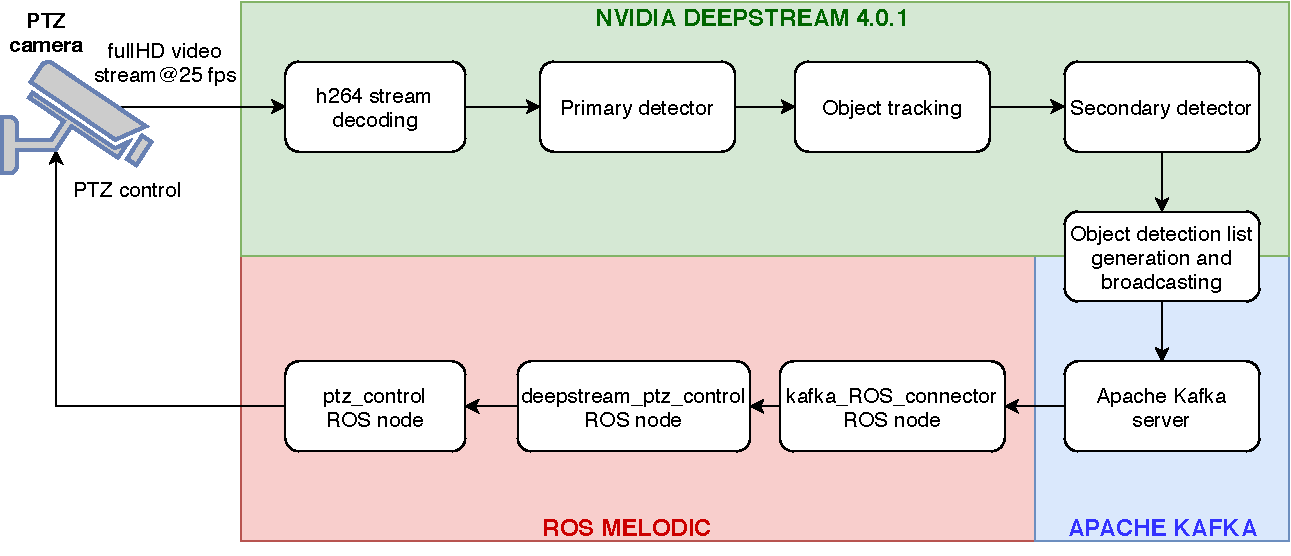
\includegraphics[width=\textwidth]{figures/tracking_with_camera.pdf}
    \caption{Camera tracking control-loop validation scenario based on the MUEAVI infrastructure. The pipeline receives a full-HD video stream from a PTZ camera, decodes it using the NVIDIA DeepStream framework, performs object detection and tracking, broadcasts object-detection messages through Apache Kafka, and converts these messages into ROS messages using the \texttt{kafka\_ROS\_connector} node. The \texttt{deepstream\_ptz\_control} ROS node computes relative pan--tilt--zoom commands from the detected-object list, while the \texttt{ptz\_control} ROS node sends the commands to the PTZ camera and publishes camera status information.}
    \label{fig:mueavi-camera-tracking}
\end{figure}

Infrastructure-supported fusion systems extend this idea by combining data from vehicle-mounted and fixed sensing sources. Roadside cameras, LiDARs, and radars can observe vehicles and vulnerable road users from viewpoints that differ from those available to the ego vehicle. This can improve object tracking, support cooperative perception, provide external validation for onboard perception, and help analyse occluded or safety-critical scenarios.

A representative infrastructure-assisted architecture consists of three layers. The first layer performs local acquisition and preprocessing close to the sensors, including video decoding, timestamping, point-cloud filtering, radar parsing, clustering, and object detection. Camera-based detection can be implemented using real-time neural detectors such as YOLOv3 \cite{redmon_yolov3_2018}. LiDAR and radar preprocessing commonly involves point-cloud filtering, downsampling, segmentation, and clustering, with tools such as the Point Cloud Library and algorithms such as DBSCAN being widely used in practical implementations \cite{rusu_pcl_2011, ester1996_dbscan}. The second layer performs centralised or distributed fusion, including coordinate transformation, multi-object tracking, object classification, sensor-selection logic, and scenario classification. The third layer supports validation, visualisation, data storage, and comparison against simulation or reference measurements.

This type of architecture connects sensor fusion with verification and validation rather than treating it as an isolated perception module. It also exposes practical implementation issues that are often hidden in algorithm-only descriptions, including time synchronisation, multi-sensor cross-calibration, middleware design, network latency, edge-computing constraints, and real-time data storage. Hardware--software co-design and systematic sensor-selection methods are therefore relevant when fusion algorithms must be deployed on embedded or resource-constrained platforms \cite{deliparaschos2016_jee_fpga}.

\subsection{Links to the Other Chapters}
\label{subsec:ch05-links}

The material of this chapter instantiates, in one application, the methods of the rest of the book. The alignment steps of Section~\ref{subsec:spatial-alignment} and the two worked examples are classical estimation problems in the sense of Chapter~\ref{sec:classicalSF}: the EKF equations \eqref{eq:kf_state_prediction}--\eqref{eq:kf_cov_update}, the consistency diagnostics \eqref{eq:nis} and the track-fusion rules \eqref{eq:independent-track-fusion-state}--\eqref{eq:ci-weight} are used unchanged. The perception side, in which detections are produced by learned camera--LiDAR--radar networks and BEV or occupancy representations, is the subject of Chapter~\ref{sec:learning}, whose hybrid architectures explain how learned detections feed the classical trackers used here. The cooperative inputs of Table~\ref{tab:av-cooperative-inputs}, the fusion of tracks across vehicles and roadside units, and the consistency problems that motivate covariance intersection in distributed settings are developed in Chapter~\ref{sec:MAS}. Finally, the issues that this chapter can only flag (calibration drift, adverse conditions, real-time embedded deployment, verification and safety assurance) are the open challenges of Chapter~\ref{sec:open-challenges}.

\problemsection

\begin{prob}\label{prob:ch05:1}
A forward camera has focal length $f_{x}=f_{y}=1200$\,pixels and a $1920\times1080$ image. Its extrinsic calibration with respect to the LiDAR has a yaw error of $0.5^{\circ}$. (a)~By how many pixels is a LiDAR point projected through \eqref{eq:lidar-to-image} displaced horizontally, and does the displacement depend on the range? (b)~What lateral position error does the same yaw error produce for an object at $20$\,m and at $80$\,m if the camera bearing is used to position it? (c)~A translation error of $10$\,cm along the camera $x$ axis is present instead: how large is the projected pixel error at $20$\,m and at $80$\,m, and what does this imply for near-field versus far-field fusion?
\end{prob}

\begin{prob}\label{prob:ch05:2}
A camera and a radar are synchronised in software with a residual time offset of $30$\,ms, and the ego vehicle drives at $20$\,m/s. (a)~Compute the apparent longitudinal misalignment between the two sensors for a static obstacle and for an oncoming vehicle travelling at $20$\,m/s. (b)~The longitudinal standard deviation of the innovation (the difference between the two detections) is $0.3$\,m; compute the normalised distance of the offset in both cases and discuss whether the gate \eqref{eq:mahalanobis_gate} with $\gamma=9.21$ ($99$\,\% for two degrees of freedom) would still associate the two detections. (c)~Propose a state augmentation that would allow the filter to estimate the offset online, and state when it is observable.
\end{prob}

\begin{prob}\label{prob:ch05:3}
Dead-reckoning drift. A vehicle drives straight at speed $v$ with a gyroscope bias $b$ that is not compensated. (a)~Show that the heading error after a time $\tau$ is $b\tau$ and the cross-track position error is approximately $vb\tau^{2}/2$. (b)~Evaluate both for $b=10$\,mrad/s, $v=14$\,m/s and $\tau=25$\,s and compare with the three-state filter of Example~\ref{ex:gnss-imu-odom}, whose error at the end of the outage is $63.9$\,m; explain the difference. (c)~A wheel scale error $s=2$\,\% is present as well: compute the along-track error after $\tau=25$\,s and the total error, and state which of the two errors would be reduced by a tactical-grade IMU.
\end{prob}

\begin{prob}\label{prob:ch05:4}
Computational. Re-run the GNSS--IMU--wheel-odometry filter of Example~\ref{ex:gnss-imu-odom} with (a)~a $60$\,s outage from $t=50$\,s and (b)~GNSS fixes at $1$\,Hz instead of $2$\,Hz before a $25$\,s outage. For each case report the position error at the end of the outage, the $3\sigma$ radius reported by the five-state filter and whether the error is inside it, and the $3\sigma$ uncertainty of the bias estimate at the tunnel entrance. Explain the dependence of the drift on the outage length and of the bias uncertainty on the GNSS rate. See \repopath{companion\_\allowbreak repo/\allowbreak exercises/\allowbreak ch05/\allowbreak }.
\end{prob}

\begin{prob}\label{prob:ch05:5}
Two tracks have identical covariances $\mathbf{P}_{1}=\mathbf{P}_{2}=\mathbf{P}$. (a)~Show that the independent rule \eqref{eq:independent-track-fusion-state} gives $\mathbf{P}_{\mathrm{f}}=\mathbf{P}/2$ whereas covariance intersection \eqref{eq:ci-cov} gives $\mathbf{P}_{\mathrm{CI}}=\mathbf{P}$ for every $\omega$. (b)~Interpret both results in terms of the information that the two tracks may share. (c)~Let the actual cross-covariance be $\mathbf{P}_{12}=\rho\mathbf{P}$ with $0\le\rho\le1$; compute the actual covariance of the naive fused estimate and its expected NEES $\tr(\mathbf{P}_{\mathrm{f}}^{-1}\mathbf{P}_{\mathrm{act}})$ as a function of $\rho$ for a two-dimensional state, and the value of $\rho$ above which the actual variance of the naive estimate exceeds the reported one by more than $50$\,\%.
\end{prob}

\begin{prob}\label{prob:ch05:6}
Computational. Starting from the script of Example~\ref{ex:camera-radar-ci}, vary the camera range accuracy $\sigma_{r}/r\in\{5,15,30\}$\,\% and the radar bearing accuracy $\sigma_{\theta}\in\{0.5,1.5,3\}^{\circ}$. For each of the nine combinations report $\omega^{\star}$, $\tr\mathbf{P}_{\mathrm{CI}}$ and $\tr\mathbf{P}_{\mathrm{f}}$ of the naive rule, and explain why $\omega^{\star}$ changes so little across the grid. Then replace the radar by an imaging radar with $\sigma_{\theta}=0.1^{\circ}$ and show what happens to $\omega^{\star}$ and to $\mathbf{P}_{\mathrm{CI}}$ when one track dominates the other in every direction. See \repopath{companion\_\allowbreak repo/\allowbreak exercises/\allowbreak ch05/\allowbreak }.
\end{prob}

\begin{prob}\label{prob:ch05:7}
Metrics. (a)~A 3D detector obtains $\mathrm{mAP}=0.60$, $\mathrm{mATE}=0.30$\,m, $\mathrm{mASE}=0.25$, $\mathrm{mAOE}=0.40$\,rad, $\mathrm{mAVE}=0.35$\,m/s and $\mathrm{mAAE}=0.15$ on nuScenes; compute its NDS with \eqref{eq:nds}. Adding a radar branch leaves all terms unchanged except $\mathrm{mAVE}=0.20$\,m/s; compute the new NDS. (b)~A tracker evaluated over $1000$ ground-truth objects misses $120$, raises $80$ false alarms and switches identity $10$ times; compute its MOTA with \eqref{eq:mota}. (c)~A classifier places $400$ predictions in the confidence bin $[0.8,0.9)$ with mean confidence $0.86$ and accuracy $0.74$, and $600$ in $[0.9,1.0]$ with mean confidence $0.95$ and accuracy $0.91$; compute its ECE with \eqref{eq:ece-metric}.
\end{prob}

\begin{prob}\label{prob:ch05:8}
Latency budget. A perception chain has $\tau_{\mathrm{sense}}=33$\,ms (camera at $30$\,Hz), $\tau_{\mathrm{xfer}}=5$\,ms, $\tau_{\mathrm{detect}}=40$\,ms, $\tau_{\mathrm{fuse}}=5$\,ms, $\tau_{\mathrm{plan}}=60$\,ms, $\tau_{\mathrm{ctrl}}=10$\,ms and $\tau_{\mathrm{act}}=150$\,ms. (a)~Compute the end-to-end latency and the distance travelled at $30$\,m/s. (b)~The fusion module receives the camera detection with an age of $\tau_{\mathrm{sense}}+\tau_{\mathrm{xfer}}+\tau_{\mathrm{detect}}$ and a radar track with an age of $15$\,ms; to which time should it predict both before fusing them, and by how much does the position uncertainty of a vehicle with unmodelled acceleration $\sigma_{a}=0.8$\,m/s$^{2}$ grow when predicted over the larger of the two ages? (c)~Pipelining the detection on two GPUs doubles the throughput: how does this change the latency, and which of the terms would have to be reduced to shorten the stopping distance?
\end{prob}




\clearpage

\clearpage

\chapter{Sensor Fusion in Multi-Agent Systems}
\label{sec:MAS}



\abstract{This chapter extends sensor fusion from a single platform to a network of vehicles, roadside units, or monitoring stations that observe the same scene and communicate only with their neighbours. It answers one question: how can such agents fuse their estimates of the same quantity without counting the same information twice and without being misled by a faulty agent? A network of five sensing nodes is used throughout. Average consensus is introduced first, in its Laplacian and Metropolis forms, with a convergence rate read from the spectrum of the graph. Building on the Kalman filter of Chapter~\ref{sec:classicalSF}, the chapter then presents the centralised filter in information form, the Kalman-consensus filter, and consensus on information, and shows on the running example that naive averaging of neighbouring estimates double-counts common information and yields overconfident covariances, whereas covariance intersection remains consistent when correlations are unknown. Trimmed (W-MSR) consensus and consistency checks protect the network against a misbehaving node, provided that the graph is sufficiently redundant. A final section summarises what changes in real networks (packet loss, delays, limited bandwidth, cooperative perception between vehicles) and how a distributed scheme should be validated; the broader literature on multi-agent estimation is indicated but not reviewed.}
\suppressfloats[t]


Several vehicles, roadside units, or monitoring stations often observe the same scene from different places. A roadside camera may see a pedestrian whom a parked truck hides from an approaching car; several coastal stations see the same vessel. Each agent runs its own estimator and can exchange information only with the agents within communication range. This chapter answers one question: how can such agents fuse their estimates of the same quantity without counting the same information twice and without being misled by an agent that is faulty?

The network of Fig.~\ref{fig:mas-network} is used throughout. Five sensing nodes, for instance roadside units around a junction, communicate along the ring $1$--$2$--$3$--$4$--$5$--$1$ and the chord $1$--$3$, and each of them observes a moving target only partially. In Example~\ref{ex:mas-network-consensus} the five nodes agree on a scalar value by consensus; in Example~\ref{ex:mas-distributed-tracking} they track the target with six fusion schemes, two of which double-count information and fail; and in Example~\ref{ex:mas-resilient-net} one of them misbehaves. After the chapter the reader should be able to (i) run average consensus with Metropolis weights and predict its convergence rate from the spectrum of the graph (Sects.~\ref{sec:mas-architectures} and~\ref{sec:mas-graph-theory}); (ii) implement a distributed Kalman filter in information form and recognise double counting through the NEES (Sect.~\ref{sec:mas-dkf}); (iii) fuse estimates whose correlation is unknown by covariance intersection (Sect.~\ref{sec:mas-unknown-corr}); and (iv) make consensus resilient to a misbehaving node, knowing which graphs allow it (Sect.~\ref{sec:mas-resilience}). Section~\ref{sec:mas-real-networks} summarises what changes in real networks and how a distributed fusion scheme should be validated.

The literature on multi-agent estimation is much broader than these four problems. Multi-robot simultaneous localisation and mapping, distributed particle filters, learned cooperative perception, and the coordination and control of the agents themselves are not treated here. Consensus and distributed estimation are surveyed in \cite{olfatisaber2007_consensus,ren2005_consensus}, and the datasets cited in Sect.~\ref{sec:mas-real-networks} are an entry point to cooperative perception between vehicles.

\begin{figure}[!t]
\centering
\begin{tikzpicture}[font=\scriptsize,
    nd/.style={circle, draw=EkfBlue!80!black, fill=EkfBlue!8, minimum size=6.5mm, inner sep=0pt, line width=0.6pt},
    lab/.style={align=center, font=\scriptsize}]
\def\R{1.45}
\coordinate (c1) at (90:\R);   \coordinate (c2) at (18:\R);   \coordinate (c3) at (-54:\R);
\coordinate (c4) at (-126:\R); \coordinate (c5) at (162:\R);
\draw[line width=0.8pt] (c1)--(c2)--(c3)--(c4)--(c5)--(c1);
\draw[line width=0.8pt] (c1)--(c3);
\draw[line width=0.6pt, densely dashed, gray] (c2)--(c4) (c2)--(c5) (c3)--(c5);
\foreach \i in {1,...,5} {\node[nd] at (c\i) {$\i$};}
\node[lab, above=4mm] at (c1) {$p_x$, $\sigma=2$\,m};
\node[lab, right=4mm] at (c2) {$p_y$, $\sigma=2$\,m};
\node[lab, right=4mm] at (c3) {$p_x$ and $p_y$, $\sigma=6$\,m};
\node[lab, left=4mm] at (c4) {$p_x$, $\sigma=3$\,m};
\node[lab, left=4mm] at (c5) {$p_y$, $\sigma=3$\,m};
\end{tikzpicture}
\caption{The running network of the chapter. Five sensing nodes communicate along the solid edges (the ring $1$--$2$--$3$--$4$--$5$--$1$ and the chord $1$--$3$); each node measures the position of a moving target only partially, with the standard deviation indicated. The dashed edges are the three links added in Sect.~\ref{subsec:mas-wmsr} to make the network resilient to one misbehaving node.}
\label{fig:mas-network}
\end{figure}

\section{Architectures and Information-Exchange Levels}
\label{sec:mas-architectures}

Architecturally, multi-agent fusion can be centralised, decentralised, or hybrid. In a centralised architecture, agents transmit measurements, features, tracks, or local maps to a fusion centre, which performs association, estimation, and decision-making. This can produce a globally consistent estimate, but it requires communication bandwidth, low enough latency, and a trusted computational node. In a decentralised architecture, each agent maintains its own estimate and exchanges selected information with neighbours. Consensus filters, distributed Kalman filters, distributed particle filters, covariance-intersection methods, and belief-function frameworks are representative tools when no single node has all information or when cross-correlations are unknown \cite{khaleghi_multisensor_2013,foglietta_networked_2012}.

Three questions determine which architecture is appropriate: who holds the global model, what is transmitted, and what is assumed about the dependence between what is received and what is already known. In a centralised scheme the fusion centre receives raw measurements that are conditionally independent given the state, so the information form of the Kalman filter of Section~\ref{sec:classicalSF} applies directly and the fused information matrix is the sum of the local contributions, as made explicit in \eqref{eq:dkf-central-info} below. In a decentralised scheme the exchanged objects are estimates, each of which already contains the common prior, the effect of the common process noise, and possibly information previously received from the same neighbours. The correlation between what an agent receives and what it already knows is therefore structural rather than accidental, and the central theme of this chapter is how to fuse correctly, or at least consistently, under this correlation.

\subsection{Communication Graphs and the Consensus Primitive}
\label{subsec:mas-graph-primitive}


The natural abstraction for decentralised fusion is a communication graph $\mathcal{G}=(\mathcal{V},\mathcal{E})$, where the node set $\mathcal{V}=\{1,\dots,N\}$ collects the agents and an edge $(i,j)\in\mathcal{E}$ indicates that agents $i$ and $j$ can exchange information directly, for example over a vehicle-to-vehicle (V2V) or vehicle-to-infrastructure (V2I) link. The \emph{neighbour set} $\mathcal{N}_i=\{j:(i,j)\in\mathcal{E}\}$ of agent $i$ therefore contains exactly the agents it can hear at a given time; no agent needs global knowledge of the network. Classical results show that if the graph is connected (or, for time-varying and directed networks, suitably jointly connected), simple local averaging rules drive all agents to agreement, with convergence speed governed by the algebraic connectivity of the graph \cite{olfatisaber2007_consensus,ren2005_consensus}.

The simplest decentralised mechanism is the consensus filter, in which each agent $i$ repeatedly averages its local estimate with those of its communication neighbours,
\begin{equation}
\widehat{\mathbf{x}}_i(k+1)=\widehat{\mathbf{x}}_i(k)+\epsilon\sum_{j\in\mathcal{N}_i}\left(\widehat{\mathbf{x}}_j(k)-\widehat{\mathbf{x}}_i(k)\right),
\label{eq:consensus-filter}
\end{equation}
where $\mathcal{N}_i$ is the neighbour set of agent $i$ and $\epsilon>0$ is a step size bounded by the inverse of the maximum node degree. Under mild connectivity assumptions, all local estimates converge to a common value, so a network can agree on a fused state using only local exchanges. In practice, consensus iterations are interleaved with local measurement updates (consensus-on-information or consensus-on-measurement filters), and when the cross-correlations between agents' estimates are unknown, the covariance-intersection rule of \eqref{eq:ci-cov}--\eqref{eq:ci-est} in Section~\ref{subsec:track-fusion} provides the consistent way to merge the exchanged estimates.



\begin{example}[Consensus on the running network]
\label{ex:mas-network-consensus}
The five nodes of Fig.~\ref{fig:mas-network} hold range estimates to a common obstacle, $\widehat{x}_1(0)=10$, $\widehat{x}_2(0)=12$, $\widehat{x}_3(0)=11$, $\widehat{x}_4(0)=15$, and $\widehat{x}_5(0)=13$\,m. Nodes $1$ and $3$ have three neighbours and the others two, so any step size $\epsilon<1/3$ is admissible; take $\epsilon=0.3$. Node~$1$, for example, computes $10+0.3\,[(12-10)+(11-10)+(13-10)]=11.8$\,m, and one application of \eqref{eq:consensus-filter} yields
\begin{equation*}
\widehat{x}_1(1)=11.8,\quad \widehat{x}_2(1)=11.1,\quad \widehat{x}_3(1)=12.2,\quad \widehat{x}_4(1)=13.2,\quad \widehat{x}_5(1)=12.7 .
\end{equation*}
The sum of the five values, $61$\,m, and hence their average, $12.2$\,m, is preserved at every iteration; continued iterations contract the spread geometrically, and all five estimates converge to $12.2$\,m although no node communicates beyond its neighbours. The outlying estimate of node~$4$ is absorbed gradually. Two caveats appear already: each fused value costs several communication rounds, whose number Sect.~\ref{subsec:mas-laplacian} computes, and a node that does not follow the iteration biases the whole network (Sect.~\ref{subsec:mas-wmsr}).
\end{example}

\subsection{Hybrid Architectures and Information-Exchange Levels}
\label{subsec:mas-levels}

Hybrid architectures are often the most practical: local edge nodes perform fast preprocessing and tracking, while a regional or cloud-level node performs slower map update, validation, learning, or fleet-level coordination \cite{deng_edge_2021,lim_federated_2020}.

The information exchanged between agents strongly affects both performance and deployability. Raw-data sharing can preserve the most information but is expensive and sensitive to synchronisation, calibration, and privacy constraints. Feature-level sharing reduces bandwidth and can support learned cooperative perception, but it requires compatible representations and careful uncertainty calibration. Object- or track-level sharing is efficient and interpretable, but it depends on reliable local detection, association, and covariance or confidence estimates. Decision-level sharing is the lightest option and is useful for warnings, alerts, or manoeuvre coordination, but it may hide the uncertainty and conflict that generated the decision. The choice of communication level is therefore a fusion-design decision, not only a networking detail. The four levels also differ in what the receiver can assume about statistical dependence: raw measurements from different platforms are conditionally independent given the state and may be summed in information form, whereas features, tracks, and decisions are outputs of local estimators that already contain shared prior knowledge. The estimation-theoretic consequences of this distinction are developed in Sections~\ref{sec:mas-dkf} and~\ref{sec:mas-unknown-corr}, and its practical embodiment in connected vehicles, where the levels are usually called early, intermediate, and late fusion, is discussed in Section~\ref{sec:mas-real-networks}.

\section{Graph-Theoretic Preliminaries and Consensus}
\label{sec:mas-graph-theory}

The consensus iteration \eqref{eq:consensus-filter} is the building block of every decentralised method in this chapter, and its behaviour is governed entirely by the spectrum of a matrix associated with the communication graph. This section collects the facts needed later; comprehensive treatments can be found in \cite{olfatisaber2007_consensus,ren2005_consensus}.

\subsection{Laplacian Form, Average Preservation, and Convergence Rate}
\label{subsec:mas-laplacian}

Let $\mathbf{A}\in\{0,1\}^{N\times N}$ be the adjacency matrix of an undirected graph, with $a_{ij}=1$ if $(i,j)\in\mathcal{E}$ and $a_{ij}=0$ otherwise, let $d_i=|\mathcal{N}_i|$ be the degree of node $i$, and let $\mathbf{D}=\diag(d_1,\dots,d_N)$. The graph Laplacian is $\mathbf{L}=\mathbf{D}-\mathbf{A}$. For scalar quantities, stacking the local values in $\mathbf{z}(k)=[\widehat{x}_1(k),\dots,\widehat{x}_N(k)]^{\mathsf T}$ turns \eqref{eq:consensus-filter} into the linear iteration
\begin{equation}
\mathbf{z}(k+1)=(\mathbf{I}-\epsilon\mathbf{L})\,\mathbf{z}(k)=\mathbf{W}\mathbf{z}(k),
\label{eq:consensus-laplacian}
\end{equation}
and vector-valued estimates are handled component-wise, i.e., with $\mathbf{W}\otimes\mathbf{I}$. Two properties of the Laplacian explain the behaviour observed in Example~\ref{ex:mas-network-consensus}. First, every row of $\mathbf{L}$ sums to zero, $\mathbf{L}\mathbf{1}=\mathbf{0}$, so a configuration in which all agents hold the same value is an equilibrium. Second, for an undirected graph $\mathbf{L}$ is symmetric, hence $\mathbf{1}^{\mathsf T}\mathbf{L}=\mathbf{0}^{\mathsf T}$ and
\begin{equation}
\mathbf{1}^{\mathsf T}\mathbf{z}(k+1)=\mathbf{1}^{\mathsf T}\mathbf{z}(k)-\epsilon\,\mathbf{1}^{\mathsf T}\mathbf{L}\mathbf{z}(k)=\mathbf{1}^{\mathsf T}\mathbf{z}(k),
\label{eq:consensus-average-preserved}
\end{equation}
so the network average $\bar{z}=\mathbf{1}^{\mathsf T}\mathbf{z}(0)/N$ is an invariant of the iteration. The Laplacian is positive semidefinite with eigenvalues $0=\lambda_1\le\lambda_2\le\dots\le\lambda_N\le 2d_{\max}$, and $\lambda_2>0$ if and only if the graph is connected; $\lambda_2$ is the \emph{algebraic connectivity}. Decomposing $\mathbf{z}(k)$ along the eigenvectors of $\mathbf{L}$ shows that the disagreement vector $\boldsymbol{\delta}(k)=\mathbf{z}(k)-\bar{z}\mathbf{1}$ satisfies
\begin{equation}
\|\boldsymbol{\delta}(k)\|\le\rho^{k}\|\boldsymbol{\delta}(0)\|,\qquad
\rho=\max\{|1-\epsilon\lambda_2|,\,|1-\epsilon\lambda_N|\},
\label{eq:consensus-rate}
\end{equation}
so the iteration converges for every $0<\epsilon<2/\lambda_N$, and since $\lambda_N\le 2d_{\max}$ the condition $\epsilon<1/d_{\max}$ quoted after \eqref{eq:consensus-filter} is a sufficient condition that requires only local degree information. The fastest constant step is $\epsilon^{\star}=2/(\lambda_2+\lambda_N)$, for which $\rho^{\star}=(\lambda_N-\lambda_2)/(\lambda_N+\lambda_2)$ \cite{xiao2004_fast_averaging}. For the running network of Example~\ref{ex:mas-network-consensus} the Laplacian eigenvalues are $0$, $1.382$, $2.382$, $3.618$, and $4.618$; with $\epsilon=0.3$ the contraction factor is $\rho=0.585$ per round, so reducing the initial disagreement by a factor of $100$ takes $9$ rounds, and the optimal step $\epsilon^{\star}=1/3$ gives $\rho^{\star}=0.539$ and $8$ rounds. Removing the edges $5$--$1$ and $1$--$3$ leaves the path $1$--$2$--$3$--$4$--$5$, whose algebraic connectivity is only $0.382$: the same step then needs $38$ rounds (Problem~\ref{prob:ch06:1}). The practical message is that sparse, elongated networks (small $\lambda_2$) agree slowly, and that each fused value costs a number of communication rounds that grows with $1/\lambda_2$.

\subsection{Metropolis Weights}
\label{subsec:mas-metropolis}

The uniform step $\epsilon$ in \eqref{eq:consensus-laplacian} is not the only choice. Any iteration of the form
\begin{equation}
\widehat{\mathbf{x}}_i(k+1)=\sum_{j\in\mathcal{N}_i\cup\{i\}}w_{ij}\,\widehat{\mathbf{x}}_j(k),\qquad w_{ij}\ge0,\quad \sum_{j}w_{ij}=1,
\label{eq:consensus-weighted}
\end{equation}
with a row-stochastic weight matrix $\mathbf{W}$ whose self-weights \DIFdelbegin \DIFdel{$w_{ii}$ are positive reaches agreement on a connected graph}\DIFdelend \DIFaddbegin \DIFadd{are positive and whose positive off-diagonal weights give a strongly connected influence graph reaches agreement}\DIFaddend , and preserves the average if $\mathbf{W}$ is also column-stochastic (doubly stochastic). A convenient doubly stochastic choice that each agent can compute from the degrees of its neighbours only is given by the \emph{Metropolis weights} \cite{xiao2005_distributed_fusion}
\begin{equation}
w_{ij}=\frac{1}{1+\max\{d_i,d_j\}}\quad\text{for } j\in\mathcal{N}_i,\qquad
w_{ii}=1-\sum_{j\in\mathcal{N}_i}w_{ij}.
\label{eq:metropolis-weights}
\end{equation}
The convergence rate is then the second largest eigenvalue modulus of $\mathbf{W}$. For the running network of Fig.~\ref{fig:mas-network} the Metropolis matrix has rows $(0.25,\allowbreak 0.25,\allowbreak 0.25,\allowbreak 0,\allowbreak 0.25)$, $(0.25,\allowbreak 0.5,\allowbreak 0.25,\allowbreak 0,\allowbreak 0)$, $(0.25,\allowbreak 0.25,\allowbreak 0.25,\allowbreak 0.25,\allowbreak 0)$, $(0,\allowbreak 0,\allowbreak 0.25,\allowbreak 0.4167,\allowbreak 0.3333)$, and $(0.25,\allowbreak 0,\allowbreak 0,\allowbreak 0.3333,\allowbreak 0.4167)$, whose second largest eigenvalue modulus is $0.6545$. Since \eqref{eq:consensus-weighted} is a convex combination of neighbouring values, we will see in Section~\ref{sec:mas-dkf} that it is also exactly the operation needed to average information matrices without double counting.

\subsection{Directed and Time-Varying Graphs}
\label{subsec:mas-directed}

Wireless links are frequently asymmetric (different transmit powers, antenna patterns, or interference), so that $\mathcal{N}_i$ must be read as the set of \emph{in-neighbours} whose messages agent $i$ receives. For a directed graph the row-stochastic iteration \eqref{eq:consensus-weighted} still reaches agreement provided that the graph contains a directed spanning tree, i.e., a root from which every agent can be reached \cite{ren2005_consensus}, but the limit is in general the weighted average $\boldsymbol{\pi}^{\mathsf T}\mathbf{z}(0)$, where $\boldsymbol{\pi}$ is the left Perron eigenvector of $\mathbf{W}$; the plain average is recovered only when $\mathbf{W}$ is doubly stochastic, which for the Laplacian form requires the digraph to be weight-balanced \cite{olfatisaber2007_consensus}. When balancing is impossible, the \emph{push-sum} or \emph{ratio-consensus} iteration runs two coupled averaging processes, one on the values and one on a vector of weights initialised at $\mathbf{1}$, and takes their ratio; the ratio converges to the exact average on any strongly connected digraph \cite{kempe2003_gossip}, and the scheme can be made robust to bounded link delays \cite{hadjicostis2014_delays}. Finally, when the topology changes with time, as happens whenever vehicles move in and out of radio range, agreement is \DIFdelbegin \DIFdel{still guaranteed if the union of the graphs over any bounded time window contains a }\DIFdelend \DIFaddbegin \DIFadd{guaranteed under uniformly positive nonzero weights, positive self-weights, and a uniform finite bound on windows whose union contains a directed }\DIFaddend spanning tree \cite{jadbabaie2003_coordination,ren2005_consensus}. In all these cases the price of a weaker topology is a slower rate, and in the worked examples below we quantify how many consensus rounds per sampling interval are needed before the distributed filter approaches the centralised one.

\section{Distributed Kalman Filtering}
\label{sec:mas-dkf}

We now combine the consensus primitive with the Kalman filter of Chapter~\ref{sec:classicalSF}. Consider the linear model \eqref{eq:kf_linear_process} with transition matrix $\mathbf{F}$ and process covariance $\mathbf{Q}$, observed by $N$ nodes through
\begin{equation}
\mathbf{y}_{i,k}=\mathbf{H}_i\mathbf{x}_k+\mathbf{r}_{i,k},\qquad \mathbf{r}_{i,k}\sim\mathcal{N}(\mathbf{0},\mathbf{R}_i),\qquad i=1,\dots,N,
\label{eq:dkf-local-measurement}
\end{equation}
with measurement noises independent across nodes and time. Individual nodes need not observe the whole state: a node may measure only one coordinate, only a range, or only a bearing, so that the pair $(\mathbf{F},\mathbf{H}_i)$ is not observable, whereas the pair $(\mathbf{F},[\mathbf{H}_1^{\mathsf T}\cdots\mathbf{H}_N^{\mathsf T}]^{\mathsf T})$ is. This situation, called \emph{collective observability}, is the typical motivation for cooperation.

\subsection{Centralised Information Form and Consensus on Measurements}
\label{subsec:mas-central-info}

Writing the Kalman update \eqref{eq:kf_state_update}--\eqref{eq:kf_cov_update} in terms of the information matrix $\mathbf{\Lambda}=\mathbf{P}^{-1}$ and the information vector $\mathbf{q}=\mathbf{\Lambda}\widehat{\mathbf{x}}$, the centralised filter that receives all $N$ measurements performs
\begin{equation}
\mathbf{\Lambda}_{k|k}=\mathbf{\Lambda}_{k|k-1}+\sum_{i=1}^{N}\mathbf{H}_i^{\mathsf T}\mathbf{R}_i^{-1}\mathbf{H}_i,\qquad
\mathbf{q}_{k|k}=\mathbf{q}_{k|k-1}+\sum_{i=1}^{N}\mathbf{H}_i^{\mathsf T}\mathbf{R}_i^{-1}\mathbf{y}_{i,k},
\label{eq:dkf-central-info}
\end{equation}
followed by the usual prediction \eqref{eq:kf_state_prediction}--\eqref{eq:kf_cov_prediction}. The sums in \eqref{eq:dkf-central-info} are $N$ times the network averages of the local pairs $(\mathbf{H}_i^{\mathsf T}\mathbf{R}_i^{-1}\mathbf{H}_i,\ \mathbf{H}_i^{\mathsf T}\mathbf{R}_i^{-1}\mathbf{y}_{i,k})$. A consensus iteration can therefore compute them: if every node runs $L$ rounds of \eqref{eq:consensus-weighted} on its local pair and multiplies the result by $N$, the centralised update is recovered exactly as $L\to\infty$, and every node ends with the centralised estimate. This is the \emph{consensus on measurements} scheme \cite{olfatisaber2005_dkf_embedded}. Its weakness is that for finite $L$ the multiplication by $N$ amplifies residual disagreement, so that the local covariances no longer bound the local errors, and it requires $N$ to be known.

\subsection{The Kalman-Consensus Filter}
\label{subsec:mas-kcf}

The Kalman-consensus filter (KCF) of Olfati-Saber \cite{olfatisaber2007_dkf} avoids multiple consensus rounds by combining a one-hop exchange of measurement information with a one-hop consensus on the predicted states. At time $k$ node $i$ forms its information contributions $\mathbf{u}_i=\mathbf{H}_i^{\mathsf T}\mathbf{R}_i^{-1}\mathbf{y}_{i,k}$ and $\mathbf{U}_i=\mathbf{H}_i^{\mathsf T}\mathbf{R}_i^{-1}\mathbf{H}_i$, broadcasts the message $(\mathbf{u}_i,\mathbf{U}_i,\bar{\mathbf{x}}_i)$, where $\bar{\mathbf{x}}_i$ is its predicted state, and aggregates the messages of the closed neighbourhood $\mathcal{J}_i=\mathcal{N}_i\cup\{i\}$,
\begin{equation}
\mathbf{u}_{\mathcal{J}_i}=\sum_{j\in\mathcal{J}_i}\mathbf{u}_j,\qquad
\mathbf{U}_{\mathcal{J}_i}=\sum_{j\in\mathcal{J}_i}\mathbf{U}_j .
\label{eq:kcf-aggregate}
\end{equation}
The estimate and covariance are then updated as
\begin{align}
\mathbf{M}_i&=\left(\mathbf{P}_i^{-1}+\mathbf{U}_{\mathcal{J}_i}\right)^{-1},\label{eq:kcf-cov}\\
\widehat{\mathbf{x}}_i&=\bar{\mathbf{x}}_i+\mathbf{M}_i\left(\mathbf{u}_{\mathcal{J}_i}-\mathbf{U}_{\mathcal{J}_i}\bar{\mathbf{x}}_i\right)+\gamma_i\,\mathbf{M}_i\sum_{j\in\mathcal{N}_i}\left(\bar{\mathbf{x}}_j-\bar{\mathbf{x}}_i\right),\qquad \gamma_i=\frac{\epsilon}{1+\|\mathbf{M}_i\|_{F}},\label{eq:kcf-state}\\
\mathbf{P}_i&\leftarrow\mathbf{F}\mathbf{M}_i\mathbf{F}^{\mathsf T}+\mathbf{Q},\qquad \bar{\mathbf{x}}_i\leftarrow\mathbf{F}\widehat{\mathbf{x}}_i .\label{eq:kcf-predict}
\end{align}
The first correction term in \eqref{eq:kcf-state} is an ordinary Kalman update with the measurements of the whole neighbourhood, which is legitimate because measurements, unlike estimates, are independent across nodes. The second term is one step of \eqref{eq:consensus-filter} applied to the predicted states, scaled by the covariance so that uncertain nodes are pulled more strongly towards their neighbours. Olfati-Saber shows that with the gain $\gamma_i$ in \eqref{eq:kcf-state} the collective error dynamics are stable and the local estimates asymptotically agree \cite{olfatisaber2007_dkf}. Note, however, that $\mathbf{M}_i$ accounts only for the measurement information and not for the consensus term, so $\mathbf{P}_i$ is not the exact error covariance of $\widehat{\mathbf{x}}_i$; in Example~\ref{ex:mas-distributed-tracking} this approximation turns out to be mildly conservative.

\subsection{Consensus on Information and Kullback--Leibler Averaging}
\label{subsec:mas-coi}

Battistelli and Chisci \cite{battistelli2014_kl_consensus} take a different route, called \emph{consensus on information} (CI filter in their terminology; we write CoI to avoid confusion with covariance intersection). Each node first performs its local correction in information form,
\begin{equation}
\mathbf{\Lambda}_i^{(0)}=\mathbf{\Lambda}_{i,k|k-1}+\mathbf{H}_i^{\mathsf T}\mathbf{R}_i^{-1}\mathbf{H}_i,\qquad
\mathbf{q}_i^{(0)}=\mathbf{q}_{i,k|k-1}+\mathbf{H}_i^{\mathsf T}\mathbf{R}_i^{-1}\mathbf{y}_{i,k},
\label{eq:coi-local}
\end{equation}
and then runs $L$ rounds of weighted averaging on the \emph{posterior} information pairs,
\begin{equation}
\mathbf{\Lambda}_i^{(\ell+1)}=\sum_{j\in\mathcal{J}_i}w_{ij}\mathbf{\Lambda}_j^{(\ell)},\qquad
\mathbf{q}_i^{(\ell+1)}=\sum_{j\in\mathcal{J}_i}w_{ij}\mathbf{q}_j^{(\ell)},\qquad \ell=0,\dots,L-1,
\label{eq:coi-consensus}
\end{equation}
with doubly stochastic weights such as \eqref{eq:metropolis-weights}, after which $\mathbf{P}_{i,k|k}=(\mathbf{\Lambda}_i^{(L)})^{-1}$, $\widehat{\mathbf{x}}_{i,k|k}=\mathbf{P}_{i,k|k}\mathbf{q}_i^{(L)}$, and the prediction step follows. The key observation is that one round of \eqref{eq:coi-consensus} is exactly the covariance-intersection rule \eqref{eq:ci-cov}--\eqref{eq:ci-est} with weights $w_{ij}$, generalised to several sources, and that for Gaussian densities this is the density that minimises the weighted sum of Kullback--Leibler divergences from the local posteriors, $\sum_{j}w_{ij}\,D_{\mathrm{KL}}(p\,\|\,p_j)$ over the fused density $p$ (the \emph{Kullback--Leibler average}). Because the information is averaged rather than summed, no piece of information is ever counted more than once, whatever the value of $L$ and whatever the correlation between the local posteriors: the resulting covariances are guaranteed consistent. Battistelli and Chisci further prove that the error dynamics are stable for any $L\ge1$ under collective observability and a connected graph \cite{battistelli2014_kl_consensus}. The price is conservatism: averaging $N$ information matrices gives roughly $1/N$ of the information that summing would give, so CoI underestimates the available information. Hybrid schemes that combine consensus on measurements and on information \cite{battistelli2015_cmci}, and the information-weighted consensus filter, which divides the prior information by $N$ before averaging so that only the prior, not the measurements, is discounted \cite{kamal2013_icf}, recover centralised performance as $L$ grows while keeping the double-counting problem under control.

\subsection{Double Counting and Overconfidence}
\label{subsec:mas-double-counting}

The most common mistake in decentralised fusion is to apply the independent-track rule \eqref{eq:independent-track-fusion-state}, i.e., to add the information matrices of the estimates received from the neighbours, as if they were independent measurements. They are not: all local estimates descend from the same prior, respond to the same process noise, and, once fusion has been performed at least once, contain information that has already travelled through the network. Adding their information matrices counts the common part once per neighbour (\emph{double counting}, also known as \emph{data incest} or \emph{rumour propagation}). If the fused result is fed back into the local filter, the information matrix is multiplied by roughly $|\mathcal{J}_i|$ at every step, the Kalman gain collapses to zero, the filter stops responding to measurements, and the reported covariance becomes meaningless. Without feedback the effect is milder but still present, because the common process noise alone correlates the local errors \cite{barshalom2011tracking}. The diagnostic of choice is the normalised estimation error squared (NEES),
\begin{equation}
\varepsilon_{i,k}=(\mathbf{x}_k-\widehat{\mathbf{x}}_{i,k})^{\mathsf T}\mathbf{P}_{i,k}^{-1}(\mathbf{x}_k-\widehat{\mathbf{x}}_{i,k}),
\label{eq:nees-mas}
\end{equation}
the state-space counterpart of the NIS \eqref{eq:nis}: for a \DIFdelbegin \DIFdel{consistent Gaussian estimator }\DIFdelend \DIFaddbegin \DIFadd{zero-mean Gaussian error with covariance exactly equal to the reported covariance }\DIFaddend of an $n_x$-dimensional state, $\varepsilon_{i,k}\sim\chi^{2}_{n_x}$ with mean $n_x$, and a mean NEES well above $n_x$ reveals an overconfident filter, while a mean well below $n_x$ reveals a conservative one. Unlike the NIS, the NEES requires ground truth and is therefore a design-time and validation tool, which is how we use it next.

\begin{example}[Distributed tracking of a constant-velocity target]
\label{ex:mas-distributed-tracking}
The five sensing nodes of the running network track a target with state $\mathbf{x}=[p_x\ p_y\ v_x\ v_y]^{\mathsf T}$ that moves according to the constant-velocity model of Example~\ref{ex:ekf-radar-cutin} with $T=0.1$\,s and $\sigma_a=0.5$\,m/s$^2$, starting from $\mathbf{x}_0=[0\ 0\ 8\ 3]^{\mathsf T}$ (metres and metres per second) for $100$ steps. The nodes form the ring $1$--$2$--$3$--$4$--$5$--$1$ with the chord $1$--$3$ of Fig.~\ref{fig:mas-network}. Every node observes the target only partially: nodes $1$ and $4$ measure $p_x$ only, with standard deviations $2$\,m and $3$\,m; nodes $2$ and $5$ measure $p_y$ only, with $2$\,m and $3$\,m; node $3$ measures both coordinates but with a standard deviation of $6$\,m. No single node can observe the state, but every closed neighbourhood can. All nodes start from the same prior with $\mathbf{P}_0=\diag(25,25,4,4)$, a common initial estimate being the typical situation when the track was initialised by one node and broadcast. We compare the centralised filter \eqref{eq:dkf-central-info}; isolated local filters; naive neighbourhood fusion, in which each node adds the information of the posteriors of its closed neighbourhood as if independent, either without feedback (the local filters keep running on their own) or with feedback (the fused result replaces the local posterior); CoI with $L=3$ rounds of Metropolis averaging per sampling interval; the KCF with $\epsilon=0.05$; and covariance intersection, in which each node fuses its posterior sequentially with those of its neighbours using \eqref{eq:ci-cov}--\eqref{eq:ci-est} with the trace-minimising weight. Table~\ref{tab:mas-distributed-tracking} reports the position RMSE, the mean NEES, and the fraction of NEES samples inside the two-sided $95\,\%$ interval $[0.48,\,11.14]$ of $\chi^{2}_{4}$, averaged over the five nodes, the $100$ steps, and $50$ Monte Carlo runs; Fig.~\ref{fig:mas-distributed-tracking} shows one run.

The results support three observations. First, the isolated filters are consistent (mean NEES $4.08$) but inaccurate, with a position RMSE of $11.6$\,m: nodes $1$, $2$, $4$, and $5$ never observe one coordinate, and their covariance correctly reflects it. Second, naive fusion is easy to implement but can fail badly. With feedback the information matrix explodes, the mean NEES reaches $4.3\times10^{7}$, and the estimate, frozen after a few steps while the target moves on, ends with an RMSE of $16.1$\,m, worse than no cooperation at all. Without feedback the RMSE is a reasonable $1.10$\,m, which is precisely what makes the method dangerous: the mean NEES of $6.70$ and the $83.6\,\%$ coverage show that the reported covariance is only about 60\,\% of the actual error covariance, and a downstream consumer such as a gating test or a collision-risk estimate would be misled. Third, the three principled schemes all reach the neighbourhood of the centralised performance ($0.80$\,m) without ever summing correlated information: CoI attains $0.92$\,m with a mean NEES of $2.02$ (conservative, as predicted by the averaging argument), the KCF $0.97$\,m with a mean NEES of $3.94$, and covariance intersection $1.02$\,m with a mean NEES of $2.87$ and a mean weight $\omega=0.54$. In steady state ($t\ge5$\,s) the gap narrows further ($0.65$\,m centralised versus $0.68$\,m for CoI, $0.75$\,m for the KCF, and $0.79$\,m for CI). Increasing the number of consensus rounds helps CoI only marginally here ($0.96$\,m for $L=1$ and $0.91$\,m for $L=10$), because the second largest eigenvalue modulus $0.6545$ of the Metropolis matrix already makes three rounds sufficient on this small, well-connected graph; on a sparser network the dependence on $L$ would be much stronger (Problem~\ref{prob:ch06:5}). The code is in \repopath{companion\_\allowbreak repo/\allowbreak examples/\allowbreak ch06\_\allowbreak distributed\_\allowbreak tracking/\allowbreak }.
\end{example}

\begin{table}[!t]
\centering
\small
\caption{Distributed tracking of Example~\ref{ex:mas-distributed-tracking}: position RMSE, mean NEES \eqref{eq:nees-mas} (expected value $4$ for a consistent filter), and fraction of NEES samples inside the $95\,\%$ interval of $\chi^{2}_{4}$, averaged over nodes, time, and $50$ Monte Carlo runs.}
\label{tab:mas-distributed-tracking}
\begin{tabular}{lrrr}
\hline
\textbf{Method} & \textbf{Position RMSE [m]} & \textbf{Mean NEES} & \textbf{In 95\,\% band} \\
\hline
Centralised Kalman filter \eqref{eq:dkf-central-info} & 0.80 & 4.25 & 95.0\,\% \\
Isolated local filters & 11.65 & 4.08 & 94.4\,\% \\
Naive neighbourhood fusion, no feedback & 1.10 & 6.70 & 83.6\,\% \\
Naive neighbourhood fusion, with feedback & 16.11 & $4.3\times10^{7}$ & 0.9\,\% \\
Consensus on information, $L=3$ \eqref{eq:coi-consensus} & 0.92 & 2.02 & 87.3\,\% \\
Kalman-consensus filter \eqref{eq:kcf-state} & 0.97 & 3.94 & 95.0\,\% \\
Covariance intersection \eqref{eq:ci-cov}--\eqref{eq:ci-est} & 1.02 & 2.87 & 94.6\,\% \\
\hline
\end{tabular}
\end{table}

\begin{figure}[!t]
\centering
\resizebox{0.99\columnwidth}{!}{
\begin{tikzpicture}
\begin{groupplot}[
    group style={group size=1 by 2, vertical sep=17mm},
    width=0.95\columnwidth,
    scale only axis,
    tick label style={font=\scriptsize},
    label style={font=\scriptsize},
    legend style={font=\scriptsize, draw=none, fill=white, fill opacity=0.85,
                  text opacity=1},
    grid=major,
    grid style={line width=0.2pt, draw=gray!25},
    axis line style={line width=0.5pt},
    tick align=outside,
    title style={font=\scriptsize, yshift=0.5mm},
]

\nextgroupplot[
    height=3.3cm,
    xlabel={$p_x$ [m]},
    ylabel={$p_y$ [m]},
    xmin=-12, xmax=95,
    ymin=-15, ymax=45,
    legend pos=north west,
    legend cell align=left,
    legend columns=2,
    title={(a) bird's-eye view, one run},
]
\addplot[only marks, mark=*, mark size=0.5pt, draw=MeasGrey, fill=MeasGrey]
    table[x=px_meas3, y=py_meas3, col sep=comma] {data/ch06/distributed_tracking.csv};
\addlegendentry{node-3 detections}
\addplot[TruthBlack, line width=1.0pt]
    table[x=px_true, y=py_true, col sep=comma] {data/ch06/distributed_tracking.csv};
\addlegendentry{ground truth}
\addplot[EkfBlue, line width=0.9pt, densely dashed]
    table[x=px_cen, y=py_cen, col sep=comma] {data/ch06/distributed_tracking.csv};
\addlegendentry{centralised}
\addplot[ZonoGreen, line width=0.9pt]
    table[x=px_coi, y=py_coi, col sep=comma] {data/ch06/distributed_tracking.csv};
\addlegendentry{node 1, CoI}

\nextgroupplot[
    height=3.3cm,
    xlabel={time $t$ [s]},
    ylabel={NEES $\varepsilon_{1,k}$},
    xmin=0, xmax=10,
    ymode=log,
    ymin=0.05, ymax=1e9,
    ytick={0.1,10,1000,1e5,1e7,1e9},
    legend pos=north west,
    legend cell align=left,
    legend columns=3,
    title={(b) NEES of node 1 against the $\chi^{2}_{4}$ interval},
]

\addplot[draw=none, fill=BandGrey, forget plot]
    coordinates {(0,0.484) (10,0.484) (10,11.143) (0,11.143)} \closedcycle;
\addplot[draw=gray!70, line width=0.5pt, densely dotted, forget plot]
    coordinates {(0,4) (10,4)};
\addplot[ManoeuvreOrange, line width=0.8pt]
    table[x=t, y=nees1_naive, col sep=comma] {data/ch06/distributed_tracking.csv};
\addlegendentry{naive, feedback}
\addplot[MeasGrey, line width=0.6pt]
    table[x=t, y=nees1_naive_nf, col sep=comma] {data/ch06/distributed_tracking.csv};
\addlegendentry{naive, no feedback}
\addplot[ZonoGreen, line width=0.6pt]
    table[x=t, y=nees1_coi, col sep=comma] {data/ch06/distributed_tracking.csv};
\addlegendentry{CoI}
\addplot[EkfBlue, line width=0.6pt]
    table[x=t, y=nees1_ci, col sep=comma] {data/ch06/distributed_tracking.csv};
\addlegendentry{CI}
\addplot[TruthBlack, line width=0.4pt, densely dashed]
    table[x=t, y=nees1_central, col sep=comma] {data/ch06/distributed_tracking.csv};
\addlegendentry{centralised}
\end{groupplot}
\end{tikzpicture}
}
\caption{Distributed tracking of a constant-velocity target by five partially observing nodes (Example~\ref{ex:mas-distributed-tracking}). (a)~Detections of the noisy node~$3$, ground truth, centralised estimate, and the estimate of node~$1$ obtained by consensus on information (CoI), although node~$1$ itself measures only $p_x$. (b)~NEES of node~$1$ on a logarithmic scale against the two-sided $95\,\%$ interval of $\chi^{2}_{4}$ (shaded) and its mean $4$ (dotted). Naive information fusion with feedback drives the NEES above $10^{5}$ within one second and beyond $10^{7}$ after about four seconds: the covariance has collapsed while the error has not. In this single run the other schemes stay mostly inside the band; CoI falls below it in about half of the samples, which shows that it is conservative, and the overconfidence of naive fusion without feedback emerges only in the Monte Carlo averages of Table~\ref{tab:mas-distributed-tracking}.}
\label{fig:mas-distributed-tracking}
\end{figure}

\section{Fusion Under Unknown Correlations}
\label{sec:mas-unknown-corr}

Example~\ref{ex:mas-distributed-tracking} illustrates that correlation between the estimates circulating in a network is the rule rather than the exception. It arises from at least four sources: a common prior (track initialisation broadcast to all nodes); a common process noise, which correlates the errors of any two filters tracking the same target even if they never communicate \cite{barshalom2011tracking}; cyclic information flow, whereby a piece of information returns to its originator after travelling around a loop of the graph; and shared auxiliary estimates such as ego-pose, calibration, or map priors in cooperative perception. Keeping track of the exact cross-covariances, as in \eqref{eq:correlated-track-fusion-state}--\eqref{eq:correlated-track-fusion-cov}, would require every node to know the complete information-sharing history of every other node, which is impractical in a dynamic network.

Covariance intersection \eqref{eq:ci-cov}--\eqref{eq:ci-est} \cite{julier1997nondivergent} resolves this by renouncing knowledge of the cross-covariance altogether: for any true cross-covariance, the fused covariance $\mathbf{P}_{\mathrm{CI}}$ upper-bounds the true error covariance of $\widehat{\mathbf{x}}_{\mathrm{CI}}$. The multi-source form, which is what one round of \eqref{eq:coi-consensus} implements, reads
\begin{equation}
\mathbf{P}_{\mathrm{CI}}^{-1}=\sum_{j\in\mathcal{J}_i}\omega_j\mathbf{P}_j^{-1},\qquad
\widehat{\mathbf{x}}_{\mathrm{CI}}=\mathbf{P}_{\mathrm{CI}}\sum_{j\in\mathcal{J}_i}\omega_j\mathbf{P}_j^{-1}\widehat{\mathbf{x}}_j,\qquad
\sum_{j\in\mathcal{J}_i}\omega_j=1,\ \ \omega_j\ge0,
\label{eq:ci-multi}
\end{equation}
and the weights may be optimised as in \eqref{eq:ci-weight} or fixed a priori, e.g., to the Metropolis weights, which trades optimality for the guarantee that all nodes converge to the same value. Problem~\ref{prob:ch06:3} works through the scalar and diagonal cases and shows that CI never claims more information than the most informative source along any direction.

When part of the error is known to be independent, CI is unnecessarily conservative. \emph{Split covariance intersection} \cite{julier2001_split_ci} decomposes each covariance into a possibly correlated part and an independent part, $\mathbf{P}_j=\mathbf{P}_j^{\mathrm{d}}+\mathbf{P}_j^{\mathrm{i}}$, inflates only the correlated part, and fuses
\begin{equation}
\mathbf{P}_{\mathrm{SCI}}^{-1}=\mathbf{\Lambda}_1(\omega)+\mathbf{\Lambda}_2(\omega),\qquad
\widehat{\mathbf{x}}_{\mathrm{SCI}}=\mathbf{P}_{\mathrm{SCI}}\left[\mathbf{\Lambda}_1(\omega)\widehat{\mathbf{x}}_1+\mathbf{\Lambda}_2(\omega)\widehat{\mathbf{x}}_2\right],
\label{eq:split-ci}
\end{equation}
where
\begin{equation}
\mathbf{\Lambda}_1(\omega)=\left(\tfrac{1}{\omega}\mathbf{P}_1^{\mathrm{d}}+\mathbf{P}_1^{\mathrm{i}}\right)^{-1},\qquad
\mathbf{\Lambda}_2(\omega)=\left(\tfrac{1}{1-\omega}\mathbf{P}_2^{\mathrm{d}}+\mathbf{P}_2^{\mathrm{i}}\right)^{-1},
\label{eq:split-ci-terms}
\end{equation}
and $\omega\in(0,1)$ is again chosen by minimising a scalar criterion of $\mathbf{P}_{\mathrm{SCI}}$.
In cooperative vehicle localisation the independent part is typically the fresh measurement noise of the local sensors and the correlated part is the propagated pose error, and split CI has been shown to retain most of the accuracy of optimal fusion while remaining consistent \cite{li2013_split_ci_vehicles}. Other bounds exist that are tighter than CI under additional assumptions, notably the inverse covariance intersection \cite{noack2017_ici}, which exploits the fact that the common information cannot exceed what either source knows. For the purposes of this book, the operational rule is simple: sum information only for quantities known to be independent (raw measurements of different sensors), use CI or its refinements for everything that has passed through an estimator, and verify with the NEES in simulation that the implemented scheme is consistent before trusting its covariances on the road.


\section{Resilience, Trust, and Security}
\label{sec:mas-resilience}

Multi-agent fusion also introduces failure modes that are less visible in single-agent systems. Communication delays can make received information stale; packet losses can create intermittent measurements; inconsistent coordinate frames can corrupt cooperative tracks; duplicated information can cause overconfident estimates; and compromised or faulty agents can inject misleading evidence. Conservative fusion methods, including covariance intersection, evidence-theoretic conflict measures, innovation monitoring, and set-membership consistency checks, are therefore valuable when cross-agent dependencies or trust levels are uncertain. In connected automated vehicles, set-membership methods have been used to support shared situational awareness under occlusion, while evidence-distance and Dempster--Shafer approaches have been applied to real-time inter-vehicle data fusion \cite{narri2021_set_membership_shared_awareness,cho_realtime_2020}.

\subsection{Fault Models and Trimmed Consensus}
\label{subsec:mas-wmsr}

Example~\ref{ex:mas-network-consensus} ended with the remark that a faulty agent biases the entire network. The consensus iteration \eqref{eq:consensus-filter} is in fact maximally fragile: a single agent that keeps broadcasting a constant value, whether through a stuck sensor, a stale buffer, or malice, acts as a \emph{stubborn} node, and since the average is preserved only among compliant agents, all compliant agents converge to the stubborn value. Fault models are usually classified by the behaviour of the misbehaving agents, from crash faults (no messages) and biased or stubborn values to \emph{Byzantine} agents that may send different, arbitrary values to different neighbours, and by their number: in the $F$-\emph{total} model at most $F$ agents misbehave in the whole network, while in the $F$-\emph{local} model at most $F$ misbehave in the neighbourhood of every compliant agent.

The \emph{weighted mean-subsequence-reduced} (W-MSR) algorithm of LeBlanc et al.\ \cite{leblanc2013_wmsr} makes the averaging rule resilient at the cost of exactness. At each round, a compliant agent $i$ sorts the values received from its neighbours, discards the (at most) $F$ values that are larger than its own and the (at most) $F$ values that are smaller than its own, obtaining a reduced neighbour set $\mathcal{R}_i(k)\subseteq\mathcal{N}_i$, and then applies \eqref{eq:consensus-filter} to the survivors,
\begin{equation}
\widehat{x}_i(k+1)=\widehat{x}_i(k)+\epsilon\sum_{j\in\mathcal{R}_i(k)}\left(\widehat{x}_j(k)-\widehat{x}_i(k)\right).
\label{eq:wmsr}
\end{equation}
\DIFdelbegin \DIFdel{Because every surviving value lies between the own value and a discarded one, no compliant agent can ever be pulled outside the interval spanned by the compliant initial values, whatever the misbehaving agents transmit. }\DIFdelend \DIFaddbegin \DIFadd{Under the $F$-local fault bound, any surviving adversarial value outside the current compliant range would have been among the discarded extremes. Provided $0<\epsilon<1/d_{\max}$, the update is a convex combination, including a positive self-weight, and every compliant value stays in the compliant initial interval. This scalar validity result does not establish validity for unrestricted component-wise vector trimming. }\DIFaddend Agreement among the compliant agents is guaranteed under the $F$-local model if the graph is $(2F+1)$-\emph{robust}, where a graph is $r$-robust if for every pair of non-empty disjoint subsets of nodes at least one of the two contains a node with at least $r$ neighbours outside its own subset \cite{leblanc2013_wmsr}. Robustness is a stronger requirement than connectivity (an $r$-robust graph is $r$-connected, but not conversely), and the price of resilience is twofold: the network must be denser, and the limit is some convex combination of the compliant initial values rather than their average. Related results for linear iterative strategies in the presence of malicious agents are given in \cite{sundaram2011_malicious}.

\begin{example}[Plain versus trimmed consensus with a misbehaving node]
\label{ex:mas-resilient-net}
Return to the five nodes of Example~\ref{ex:mas-network-consensus}, with the same initial values, and let node~$5$ be faulty: from the first round it ignores the protocol and broadcasts the constant value $30$\,m. \DIFdelbegin \DIFdel{W-MSR with $F=1$ requires a }\DIFdelend \DIFaddbegin \DIFadd{A }\DIFaddend $3$-robust graph \DIFaddbegin \DIFadd{is a sufficient topology condition for W-MSR with $F=1$ under the $F$-local model}\DIFaddend , and a brute-force check over all pairs of disjoint subsets shows that the running network is only $1$-robust: for $S_1=\{1,2,3\}$ and $S_2=\{4,5\}$ no node has more than one neighbour outside its own subset. Problem~\ref{prob:ch06:7} shows what goes wrong on it. Adding the three links $2$--$4$, $2$--$5$, and $3$--$5$ (dashed in Fig.~\ref{fig:mas-network}) makes the network $3$-robust, and no set of one or two added links does; resilience to a single misbehaving node thus requires all nodes but two to hear every other node. On the densified network, with $\epsilon=0.2<1/4$, plain consensus drags the four compliant nodes to $14.6$, $15.6$, $15.6$, and $16.6$\,m after one round, to $28.1$\,m after $10$ rounds, and to $30$\,m in the limit. Under W-MSR the compliant nodes move to $10.6$, $12.4$, $12.0$, and $14.4$\,m after one round and agree on $13.33$\,m after $20$ rounds, inside the interval $[10,15]$ of their initial values. Node~$5$ is never identified, and the price paid is that the limit differs from the average $12.0$\,m of the compliant initial values. Fig.~\ref{fig:mas-resilient-net} shows both iterations; the code, including the robustness checks, is in \repopath{companion\_\allowbreak repo/\allowbreak examples/\allowbreak ch06\_\allowbreak resilient\_\allowbreak consensus/\allowbreak }.
\end{example}

\begin{figure}[!t]
\centering
\resizebox{0.99\columnwidth}{!}{
\begin{tikzpicture}
\begin{groupplot}[
    group style={group size=2 by 1, horizontal sep=14mm},
    width=0.46\columnwidth,
    height=3.4cm,
    scale only axis,
    tick label style={font=\scriptsize},
    label style={font=\scriptsize},
    legend style={font=\scriptsize, draw=none, fill=white, fill opacity=0.85, text opacity=1},
    grid=major,
    grid style={line width=0.2pt, draw=gray!25},
    axis line style={line width=0.5pt},
    tick align=outside,
    title style={font=\scriptsize, yshift=0.5mm},
    xmin=0, xmax=40, ymin=8, ymax=32,
    xlabel={round $k$},
]
\nextgroupplot[ylabel={range estimate [m]}, title={(a) plain consensus \eqref{eq:consensus-filter}}, legend pos=south east]
\addplot[draw=gray!70, line width=0.5pt, densely dotted, forget plot] coordinates {(0,12.0) (40,12.0)};
\addplot[ManoeuvreOrange, line width=1.0pt] table[x=k, y=plain5, col sep=comma] {data/ch06/resilient_consensus.csv};
\addlegendentry{node 5 (faulty)}
\addplot[EkfBlue, line width=0.6pt] table[x=k, y=plain1, col sep=comma] {data/ch06/resilient_consensus.csv};
\addlegendentry{compliant nodes}
\addplot[EkfBlue, line width=0.6pt, forget plot] table[x=k, y=plain2, col sep=comma] {data/ch06/resilient_consensus.csv};
\addplot[EkfBlue, line width=0.6pt, forget plot] table[x=k, y=plain3, col sep=comma] {data/ch06/resilient_consensus.csv};
\addplot[EkfBlue, line width=0.6pt, forget plot] table[x=k, y=plain4, col sep=comma] {data/ch06/resilient_consensus.csv};
\nextgroupplot[title={(b) W-MSR \eqref{eq:wmsr} with $F=1$}]
\addplot[draw=gray!70, line width=0.5pt, densely dotted, forget plot] coordinates {(0,12.0) (40,12.0)};
\addplot[ManoeuvreOrange, line width=1.0pt, forget plot] table[x=k, y=wmsr5, col sep=comma] {data/ch06/resilient_consensus.csv};
\addplot[EkfBlue, line width=0.6pt, forget plot] table[x=k, y=wmsr1, col sep=comma] {data/ch06/resilient_consensus.csv};
\addplot[EkfBlue, line width=0.6pt, forget plot] table[x=k, y=wmsr2, col sep=comma] {data/ch06/resilient_consensus.csv};
\addplot[EkfBlue, line width=0.6pt, forget plot] table[x=k, y=wmsr3, col sep=comma] {data/ch06/resilient_consensus.csv};
\addplot[EkfBlue, line width=0.6pt, forget plot] table[x=k, y=wmsr4, col sep=comma] {data/ch06/resilient_consensus.csv};
\end{groupplot}
\end{tikzpicture}
}
\caption{Resilient consensus on the densified running network (Example~\ref{ex:mas-resilient-net}): four compliant nodes and node~$5$, which keeps broadcasting $30$\,m. (a)~Plain consensus: the compliant nodes converge to the faulty value. (b)~W-MSR with $F=1$: the compliant nodes agree on $13.33$\,m, inside the range of their initial values; the dotted line is their initial average $12.0$\,m.}
\label{fig:mas-resilient-net}
\end{figure}

\subsection{Consistency Checks and Trust}
\label{subsec:mas-trust}

Trimmed consensus protects scalar agreement, but most of the information exchanged in multi-agent fusion consists of tracks with covariances, for which the natural defence is a consistency check before fusion. A received estimate $(\widehat{\mathbf{x}}_j,\mathbf{P}_j)$ is compared with the local prediction $(\widehat{\mathbf{x}}_{i,k|k-1},\mathbf{P}_{i,k|k-1})$ through the Mahalanobis distance of \eqref{eq:track-mahalanobis}; \DIFdelbegin \DIFdel{under the hypothesis that }\DIFdelend \DIFaddbegin \DIFadd{if }\DIFaddend both refer to the same object and \DIFdelbegin \DIFdel{that both are consistent}\DIFdelend \DIFaddbegin \DIFadd{their difference is zero-mean Gaussian with the covariance used in the test}\DIFaddend , the distance is \DIFdelbegin \DIFdel{$\chi^{2}_{n_x}$}\DIFdelend \DIFaddbegin \DIFadd{$\chi^2_{n_x}$}\DIFaddend -distributed\DIFaddbegin \DIFadd{. For correlated errors the difference covariance is $P_i+P_j-P_{ij}-P_{ij}^{\mathsf T}$; the independent sum is not an exact gate under unknown dependence. Conservative inputs alone do not give an exact chi-square distribution}\DIFaddend , and a value beyond the $99\,\%$ quantile flags the received track as suspicious. The same statistic, applied to the measurement innovation, underlies the innovation-based detection of stealthy disturbance attacks in \cite{oliva_innovation_2026}. A single rejection is not evidence of malice, because the test also fires on genuine association errors and manoeuvres (Example~\ref{ex:ekf-radar-cutin}), so the outcomes are accumulated into a trust score per neighbour, for instance $\tau_j(k+1)=\alpha\tau_j(k)+(1-\alpha)\,\mathbb{1}[\text{check passed at }k]$ with a forgetting factor $\alpha\in(0,1)$, and the trust is used to modulate the fusion weights, e.g., $\omega_j\propto\tau_j$ in \eqref{eq:ci-multi}, or to exclude a neighbour altogether. Evidence theory offers a complementary route: the conflict $K$ of Dempster's rule \eqref{eq:dempster} between the basic belief assignment received from a neighbour and the local one measures how incompatible the two sources are, and evidence-distance-based discounting of conflicting sources has been applied to real-time inter-vehicle fusion in \cite{cho_realtime_2020}. Whatever the mechanism, three principles apply: the check must be performed on the information actually received, not on a self-reported quality flag; a conservative fusion rule such as CI limits the damage of an undetected fault only if the received covariance is honest: CI weights each source by the information it declares, so a malicious sender that declares a small covariance can still dominate the fused estimate, which is why the consistency check on the received information must come first; and the system should degrade to the local estimate, never below it, when trust is lost.

\section{From the Core to Real Networks}
\label{sec:mas-real-networks}

The filters of Sect.~\ref{sec:mas-dkf} assume that every message is delivered within the sampling interval. Real vehicle-to-everything (V2X) and robotic links lose packets, deliver them late, and carry a limited number of bits, and each imperfection has an estimation-theoretic counterpart. A lost measurement simply skips the Kalman update; for unstable dynamics there is a critical arrival probability below which the expected covariance diverges \cite{sinopoli2004_intermittent}, whereas for the constant-velocity model of the running example \DIFdelbegin \DIFdel{any positive arrival rate keeps it bounded }\DIFdelend \DIFaddbegin \DIFadd{a positive independent arrival probability with full-position observations gives a bounded expected covariance}\DIFaddend , at the cost of accuracy. \DIFaddbegin \DIFadd{A positive long-run arrival fraction alone is insufficient when loss bursts can be arbitrarily long. }\DIFaddend In the consensus iterations a lost message is handled by renormalising the weights over the messages actually received: each round is still a convex combination of posteriors, hence still consistent, but the average is no longer preserved (Problem~\ref{prob:ch06:6}). A delayed message is an out-of-sequence measurement, to be processed by retrodiction \cite{barshalom2002_oosm} after the time alignment \eqref{eq:track-time-alignment-state} of Chapter~\ref{sec:classicalSF}. Bandwidth is saved by event-triggered transmission, which sends a message only when the innovation is large \cite{trimpe2014_event_based}, and by quantisation\DIFdelbegin \DIFdel{, whose error of variance $\Delta^{2}/12$ can be absorbed into }\DIFdelend \DIFaddbegin \DIFadd{. An independent uniform quantisation-error approximation has variance $\Delta^2/12$ and can be included in }\DIFaddend $\mathbf{R}$\DIFdelbegin \DIFdel{but which prevents plain consensus from preserving }\DIFdelend \DIFaddbegin \DIFadd{; deterministic quantisation may be state dependent and correlated, and does not generally preserve }\DIFaddend the exact average \cite{kashyap2007_quantized}. For the four-dimensional state of the running example, a Kalman-consensus message carries $18$ scalars per sampling interval and each round of consensus on information carries $14$, against the $n_y$ scalars of a raw measurement.

Connected and automated vehicles are the most active application of these ideas. The exchange levels of Sect.~\ref{subsec:mas-levels} appear there as early fusion of raw point clouds or images, which requires tens of megabits per second per vehicle and sub-decimetre, sub-millisecond alignment; as intermediate fusion of learned feature maps; and as late fusion of object lists, which needs some tens of kilobits per second and feeds directly into the track-to-track fusion of Sect.~\ref{subsec:track-fusion}. Three difficulties are specific to vehicles. The relative pose of sender and receiver is uncertain: a $0.5^{\circ}$ heading error at $50$\,m displaces a received object by $0.44$\,m, and this error is common to all the objects of one sender, which is the situation for which split covariance intersection \eqref{eq:split-ci} was designed. Clocks must be aligned, and the latency of every message converted into a prediction step. Finally, the same object is seen by several senders, so received tracks must be associated before fusion and fused with covariance intersection rather than by adding information; set-membership methods offer guaranteed consistency for the same task \cite{narri2021_set_membership_shared_awareness,narri2025_set_based_awareness}. The public benchmarks OPV2V \cite{xu2022_opv2v}, V2X-Sim \cite{li2022_v2xsim}, and DAIR-V2X \cite{yu2022_dairv2x} allow the three levels to be compared.

Validation must vary the communication as well as the sensing. The examples of this chapter suggest a minimal protocol: for every candidate scheme, report the accuracy (RMSE per node), the consistency (mean NEES and coverage of the $\chi^{2}$ interval over Monte Carlo runs), the disagreement between nodes, and the communication cost in messages and scalars per sampling interval, along a scenario matrix that includes at least one topology with small algebraic connectivity, one packet-loss rate above the design value, one delay longer than the sampling interval, and one misbehaving node. A scheme whose NEES is acceptable in the nominal case but not along the matrix is not validated.

\problemsection

\begin{prob}\label{prob:ch06:1}
(Convergence rate of consensus.) For the running network of Fig.~\ref{fig:mas-network}, whose Laplacian eigenvalues are $0$, $1.382$, $2.382$, $3.618$, and $4.618$, use \eqref{eq:consensus-rate} to compute the contraction factor $\rho$ for $\epsilon=0.3$, the number of rounds needed to reduce the initial disagreement $\|\boldsymbol{\delta}(0)\|$ by a factor of $100$, the optimal constant step $\epsilon^{\star}$, and the corresponding $\rho^{\star}$. Repeat for the path $1$--$2$--$3$--$4$--$5$ obtained by removing the edges $5$--$1$ and $1$--$3$, whose Laplacian eigenvalues are $2-2\cos(\pi m/5)$, $m=0,\dots,4$. Explain why in both cases $\epsilon^{\star}$ lies on the boundary of the sufficient condition $\epsilon<1/d_{\max}$ without compromising convergence.
\end{prob}

\begin{prob}\label{prob:ch06:2}
(Average preservation on directed graphs.) Show that for an undirected graph the iteration \eqref{eq:consensus-laplacian} preserves the network average, and that the weighted iteration \eqref{eq:consensus-weighted} preserves it if and only if $\mathbf{W}$ is column-stochastic. Then consider three agents with the row-stochastic weight matrix
\begin{equation*}
\mathbf{W}=\begin{bmatrix}1/2&1/2&0\\ 1/3&1/3&1/3\\ 0&1/2&1/2\end{bmatrix}
\end{equation*}
and initial values $\mathbf{z}(0)=[10\ 12\ 11]^{\mathsf T}$. Compute the left Perron eigenvector $\boldsymbol{\pi}$ of $\mathbf{W}$ (normalised so that $\boldsymbol{\pi}^{\mathsf T}\mathbf{1}=1$), the consensus value $\boldsymbol{\pi}^{\mathsf T}\mathbf{z}(0)$, and compare it with the average $11$.
\end{prob}

\begin{prob}\label{prob:ch06:3}
(Covariance-intersection weight.) Two estimates of a scalar quantity have variances $P_1=1$ and $P_2=4$. Write $P_{\mathrm{CI}}(\omega)$ from \eqref{eq:ci-cov}, find the weight that minimises it, and interpret the result. Repeat for the two-dimensional case $\mathbf{P}_1=\diag(1,4)$ and $\mathbf{P}_2=\diag(4,1)$ with the trace criterion of \eqref{eq:ci-weight}: find $\omega^{\star}$ and $\mathbf{P}_{\mathrm{CI}}$ and compare them with the independent-fusion covariance of \eqref{eq:independent-track-fusion-state}.
\end{prob}

\begin{prob}\label{prob:ch06:4}
(Double counting of a common prior.) Two nodes share a scalar prior with variance $1$ and each measures the same quantity once with noise variance $1$. Compute the posterior variance of each node, the variance claimed by the naive sum of the two posterior information values, the correct centralised posterior variance, and the \emph{actual} error variance of the naive estimate. Deduce the expected NEES of the naive estimate and comment on the result in the light of Example~\ref{ex:mas-distributed-tracking}.
\end{prob}

\begin{prob}\label{prob:ch06:5}
(Computational: consensus rounds and topology.) Using the script of Example~\ref{ex:mas-distributed-tracking}, rerun the consensus-on-information filter with $L\in\{1,3,10\}$ rounds, first on the original graph and then on the path graph $1$--$2$--$3$--$4$--$5$ (ring and chord removed), and report RMSE and mean NEES. Explain the dependence on $L$ through the second largest eigenvalue modulus of the Metropolis matrix of each graph. See \repopath{companion\_\allowbreak repo/\allowbreak exercises/\allowbreak ch06/\allowbreak }.
\end{prob}

\begin{prob}\label{prob:ch06:6}
(Computational: packet loss.) Modify the consensus-on-information filter of Example~\ref{ex:mas-distributed-tracking} so that each message is lost independently with probability $p\in\{0,0.3,0.6\}$ and each node renormalises its Metropolis weights over the messages actually received. Report RMSE and mean NEES for each $p$ and \DIFdelbegin \DIFdel{verify numerically whether consistency is preserved}\DIFdelend \DIFaddbegin \DIFadd{assess whether these finite-sample diagnostics suggest over-reported or under-reported uncertainty. Explain why they do not prove matrix consistency}\DIFaddend . See \repopath{companion\_\allowbreak repo/\allowbreak exercises/\allowbreak ch06/\allowbreak }.
\end{prob}

\begin{prob}\label{prob:ch06:7}
(Robustness of the running network.) Show that the running network of Fig.~\ref{fig:mas-network} is not $2$-robust by exhibiting two disjoint subsets of nodes in which no node has two neighbours outside its own subset, so that W-MSR with $F=1$ comes with no guarantee on it. Then (computationally, see \repopath{companion\_\allowbreak repo/\allowbreak exercises/\allowbreak ch06/\allowbreak }) run W-MSR with $F=1$ and $\epsilon=0.3$ on it, with the initial values of Example~\ref{ex:mas-network-consensus} and node~$5$ broadcasting $30$\,m, and describe what happens to the compliant nodes.
\end{prob}




\clearpage

\clearpage

\chapter{Applications Beyond Autonomous Vehicles}
\label{sec:applications}




\abstract{This chapter shows how the classical fusion toolbox of Chapter~\ref{sec:classicalSF} is assembled into complete monitoring systems outside autonomous driving. Two case studies are developed: maritime anomaly detection for the protection of critical infrastructure, and model-based monitoring of submarine cables with distributed acoustic sensing. In the first, AIS reports and coastal-radar plots are fused by a constant-velocity Kalman filter, and the innovation sequence is monitored with per-step, sliding-window and whiteness tests; a runnable example shows that a slow spoofing ramp and a coloured disturbance are exposed by different statistics. Behavioural features, route graphs and heterogeneous cues are then combined with evidence theory, whose conflict mass becomes an operator-relevant signal, and the resulting alerts are prioritised with AHP-weighted multi-criteria scores. In the second study, a damped tensioned-string model is reduced to a modal state space, the strain read by a fibre on a cable laid along a curved route is shown to be quadratic in the state, and an extended Kalman filter with a second-order measurement prediction with windowed chi-square tests detects and localises a lateral load along the cable. Worked numerical examples, figures generated by the companion repository, and end-of-chapter problems accompany both studies, and a closing paragraph draws the common pattern with the autonomous-driving pipeline: the same tools, applied to different sensors.}
\suppressfloats[t]


The two case studies in this section are deliberately chosen to show how \emph{all} the classical ingredients of Chapter~\ref{sec:classicalSF} --- Kalman filtering and innovation monitoring, evidence-theoretic conflict handling, and MCDM-based prioritisation --- combine into complete fusion systems in a domain far from autonomous driving. They should be read as integrative worked examples of the survey's toolbox rather than as an exhaustive treatment of maritime sensing.

\section{Maritime Anomaly Detection and Infrastructure Protection}

Maritime anomaly detection is a representative application in which sensor fusion is needed because no single information source provides a complete and trustworthy maritime picture. The Automatic Identification System (AIS) provides vessel identity, position, speed, course, and other navigation information, but AIS messages can be missing, delayed, spoofed, or intentionally misleading. Coastal radar, electro-optical and infrared cameras, satellite imagery, synthetic-aperture radar, hydrophones, and distributed acoustic sensing can provide independent observations, but each modality has different coverage, resolution, latency, and false-alarm characteristics. Recent surveys of AIS anomaly detection highlight the diversity of abnormal behaviours that must be considered, including route deviation, loitering, unexpected stops, speed anomalies, encounter anomalies, and suspicious gaps in transmission \cite{wolsing_anomaly_2022}. This problem is becoming more relevant as maritime navigation systems become increasingly digital and interconnected, exposing the fused navigation pipeline itself to faults, spoofing, and cyber--physical disturbances \cite{oliva_innovation_2026}.
\subsection{Sources and Their Failure Modes}
AIS is a cooperative, self-reported source: each vessel broadcasts position reports (message types 1--3 for class~A transponders, type~18 for class~B) containing the Maritime Mobile Service Identity (MMSI), the GNSS-derived latitude and longitude, speed over ground (SOG), course over ground (COG), true heading, rate of turn and navigational status, together with static and voyage-related messages (type~5) that carry the vessel name, call sign, dimensions, type, draught and destination \cite{itu_m1371_2014}. The nominal reporting interval of a class~A transponder depends on the kinematic regime: 3\,min when anchored or moored, 10\,s between 0 and 14\,kn, $6$\,s between 14 and 23\,kn, and 2\,s above 23\,kn, with the interval shortened when the vessel is changing course. Because the reports are unauthenticated and the receiving chain is passive, the AIS channel can fail in several characteristic ways: \emph{gaps} (transmitter switched off, VHF shadowing, or satellite-AIS revisit limits), \emph{identity inconsistencies} (an MMSI used by two hulls, or a static message that contradicts the observed size), \emph{kinematic inconsistencies} (reported SOG and COG incompatible with the displacement between consecutive positions), and \emph{spoofing}, in which forged or replayed messages place a vessel where it is not \cite{balduzzi_ais_2014}. The last two are the most insidious because a well-designed spoof respects the vessel dynamics and therefore passes the plausibility checks applied to a single source \cite{riveiro_review_2018}.

Non-cooperative sources are needed to close this gap. Coastal radar produces plots with range and bearing noise that, converted to Cartesian coordinates, grows with range; typical plot-to-plot standard deviations of a few tens of metres at 10--20\,km are common for X-band shore installations. Electro-optical and infrared cameras provide identity cues (silhouette, gear on deck, wake) over short ranges and in favourable visibility; satellite synthetic-aperture radar provides wide-area snapshots with revisit times of hours, which is why imagery is best used to confirm an existing track rather than to initiate one \cite{chen_sviadf_2025}. Distributed acoustic sensing on seabed fibres, discussed in Section~\ref{subsec:das-measurement-model}, adds a non-cooperative source that observes vessels only through the strain they induce in the cable, and whose spatial support is the cable itself. The design question addressed by the rest of this section is how to make these sources check one another.


The practical difficulty is that suspicious behaviour is not always dramatic. A vessel may keep transmitting AIS in order to avoid immediate suspicion while still performing small route deviations, abnormal speed profiles, unusual loitering, or manoeuvres close to protected infrastructure. This is especially relevant in congested and geopolitically sensitive regions such as the Baltic Sea, where normal maritime traffic coexists with dense networks of submarine power and communication cables. A maritime fusion architecture should therefore combine trajectory analysis with contextual information: proximity to coastlines, shipping lanes, restricted areas, cable corridors, anchorages, recent incidents, weather, and vessel class.

At the trajectory level, fusion typically starts by constructing vessel tracks from AIS and radar measurements, associating visual or satellite detections with those tracks, and extracting behavioural features such as speed over ground, course change, distance from shipping lanes, proximity to restricted areas, encounter geometry, and consistency between reported identity and observed motion. Remote-sensing imagery and AIS can also be fused to identify small vessels or vessels whose reported AIS state is inconsistent with the observed scene \cite{chen_sviadf_2025}. Graph-based route models provide an additional layer of context: a recent Baltic Sea framework constructs a Probabilistic Roadmap (PRM) of feasible maritime corridors, projects AIS trajectories onto this graph, and derives interpretable features such as route inefficiency, deviation from learned corridors, and speed or dwell time near submarine cables \cite{oliva_tomei_prm_access_2026}. This illustrates a broader design principle: raw trajectories become more informative when fused with geospatial constraints and infrastructure maps.
\subsection{Track-Level Fusion of AIS and Radar}
\label{subsec:ais-radar-track-fusion}
The computations are carried out in a local east--north--up (ENU) frame with origin at the sensor site, so that the AIS latitude--longitude pairs and the radar range--bearing plots are first mapped to planar coordinates $(p_E,p_N)$. With the state $\mathbf{x}_k=[\,p_{E,k}\;\;p_{N,k}\;\;v_{E,k}\;\;v_{N,k}\,]^{\mathsf T}$, a merchant vessel in transit is well described by the constant-velocity (CV) model \eqref{eq:kf_linear_process} with
\begin{equation}
\mathbf{F}=
\begin{bmatrix}
\mathbf{I}_2 & T\mathbf{I}_2\\ \mathbf{0} & \mathbf{I}_2
\end{bmatrix},
\qquad
\mathbf{Q}=\sigma_a^{2}
\begin{bmatrix}
\tfrac{T^{4}}{4}\mathbf{I}_2 & \tfrac{T^{3}}{2}\mathbf{I}_2\\[2pt]
\tfrac{T^{3}}{2}\mathbf{I}_2 & T^{2}\mathbf{I}_2
\end{bmatrix},
\label{eq:ch07-cv-model}
\end{equation}
where $T$ is the report period and $\sigma_a$ \DIFdelbegin \DIFdel{bounds the unmodelled acceleration }\DIFdelend \DIFaddbegin \DIFadd{is the standard deviation of an independent acceleration held constant over each interval}\DIFaddend ; manoeuvring vessels are better served by a coordinated-turn (CT) model in which the velocity vector rotates at a turn rate $\omega$, $v_{E,k+1}=v_{E,k}\cos\omega T-v_{N,k}\sin\omega T$ and $v_{N,k+1}=v_{E,k}\sin\omega T+v_{N,k}\cos\omega T$, either with $\omega$ appended to the state or through the multiple-model filters recalled in Chapter~\ref{sec:classicalSF} \cite{barshalom2001_estimation}. Both AIS and radar observe the position, $\mathbf{H}=[\,\mathbf{I}_2\;\;\mathbf{0}\,]$, with $\mathbf{R}_{\mathrm{AIS}}=\sigma_{\mathrm{AIS}}^{2}\mathbf{I}_2$ and $\mathbf{R}_{\mathrm{rad}}=\sigma_{\mathrm{rad}}^{2}\mathbf{I}_2$ (the latter obtained, in practice, by linearising the polar plot covariance at the current range). When the two sources arrive within the same period they are processed sequentially, the radar plot first and the AIS report second, each with its own innovation $\boldsymbol{\nu}_k$ and covariance $\mathbf{S}_k$ from \eqref{eq:kf_innovation}--\eqref{eq:kf_innovation_covariance}; the two innovations are mutually uncorrelated under a correct model, so their NIS values \eqref{eq:nis} add to a $\chi^{2}_{4}$ variable.

Association is performed before the update. A radar plot $j$ is assigned to a track only if it falls inside the gate \eqref{eq:mahalanobis_gate}, $\boldsymbol{\nu}_{k,j}^{\mathsf T}\mathbf{S}_{k,j}^{-1}\boldsymbol{\nu}_{k,j}\le\gamma$, with $\gamma=\chi^{2}_{2}(0.99)=9.21$ for a two-dimensional plot; AIS reports are associated by MMSI, but their position is still gated against the radar-supported prediction, and a report that fails the gate while its MMSI matches is precisely the signature of an identity or position inconsistency that the evidence layer of Section~\ref{subsec:maritime-evidence} will consume. In dense traffic, nearest-neighbour assignment is replaced by the probabilistic data association rules of Section~\ref{subsec:track-fusion}.

\subsection{Innovation-Based Monitoring of the Navigation Pipeline}
\label{subsec:maritime-innovation-monitoring}
Under a correct linear--Gaussian model the innovation sequence is zero-mean, Gaussian, white, and has covariance $\mathbf{S}_k$ \cite{barshalom2001_estimation,mehra_identification_1970}. Each of these properties yields a test, and the tests are not equivalent. The per-step NIS test flags sample $k$ when $d_k^{2}=\boldsymbol{\nu}_k^{\mathsf T}\mathbf{S}_k^{-1}\boldsymbol{\nu}_k>\chi^{2}_{n_y}(1-\alpha)$. The \emph{sliding-window} test accumulates $W$ consecutive values,
\DIFdelbegin \begin{displaymath}
\DIFdel{\begin{aligned}
&\epsilon_{k}^{W}=\sum_{i=k-W+1}^{k} d_i^{2}\;\sim\;\chi^{2}_{W n_y}\quad\text{under } \mathcal{H}_0,\\
&\text{alarm if } \epsilon_{k}^{W}>\chi^{2}_{W n_y}(1-\alpha)\;\text{ or }\;\epsilon_{k}^{W}<\chi^{2}_{W n_y}(\alpha),
\end{aligned}
%DIFDELCMD < \label{eq:ch07-window-nis}%%%
}\end{displaymath}%DIFAUXCMD
\DIFdelend \DIFaddbegin \begin{equation}
\DIFadd{\begin{aligned}
&\epsilon_{k}^{W}=\sum_{i=k-W+1}^{k} d_i^{2}\;\sim\;\chi^{2}_{W n_y}\quad\text{under } \mathcal{H}_0,\\
&\text{alarm if } \epsilon_{k}^{W}>\chi^{2}_{W n_y}(1-\alpha/2)\;\text{ or }\;\epsilon_{k}^{W}<\chi^{2}_{W n_y}(\alpha/2),
\end{aligned}
\label{eq:ch07-window-nis}
}\end{equation}\DIFaddend 
where the two-sided form matters: an innovation that is systematically \emph{too small} is as much a symptom of model mismatch (an over-estimated $\mathbf{R}$, or a filter that is following a slowly varying disturbance) as one that is too large. The \emph{whiteness} test examines the sample autocorrelation of the whitened innovation components $\tilde{\nu}_{k,i}$, with $\tilde{\boldsymbol{\nu}}_k=\mathbf{S}_k^{-1/2}\boldsymbol{\nu}_k$,
\DIFdelbegin \begin{displaymath}
\DIFdel{\hat\rho_{i}(\ell)=\frac{\sum_{k=\ell+1}^{M}\tilde{\nu}_{k,i}\tilde{\nu}_{k-\ell,i}}{\sum_{k=1}^{M}\tilde{\nu}_{k,i}^{2}},
\qquad
Q_{\mathrm{LB}}=M(M+2)\sum_{i=1}^{n_y}\sum_{\ell=1}^{L}\frac{\hat\rho_{i}(\ell)^{2}}{M-\ell}\;\sim\;\chi^{2}_{n_y L},
%DIFDELCMD < \label{eq:ch07-ljung-box}%%%
}\end{displaymath}%DIFAUXCMD
\DIFdelend \DIFaddbegin \begin{equation}
\DIFadd{\hat\rho_{i}(\ell)=\frac{\sum_{k=\ell+1}^{M}\tilde{\nu}_{k,i}\tilde{\nu}_{k-\ell,i}}{\sum_{k=1}^{M}\tilde{\nu}_{k,i}^{2}},
\qquad
Q_{\mathrm{LB}}=M(M+2)\sum_{i=1}^{n_y}\sum_{\ell=1}^{L}\frac{\hat\rho_{i}(\ell)^{2}}{M-\ell}\;\dot\sim\;\chi^{2}_{n_y L},
\label{eq:ch07-ljung-box}
}\end{equation}\DIFaddend 
computed over the last $M$ innovations and $L$ lags; this is the Ljung--Box portmanteau statistic \cite{ljung_box_1978}, applied component-wise and summed. \DIFaddbegin \DIFadd{This approximation assumes nominally independent standardised components and a sufficiently long window; parameters fitted on the same record and small windows affect its calibration. It tests within-component serial correlation and can miss cross-component lagged dependence. }\DIFaddend A bias $\mathbf{b}$ in the innovation turns $d_k^{2}$ into a non-central $\chi^{2}$ variable with non-centrality $\lambda=\mathbf{b}^{\mathsf T}\mathbf{S}^{-1}\mathbf{b}$; the per-step test sees $\lambda$ once, whereas the windowed statistic sees $W\lambda$ against a threshold that grows only like $W n_y+O(\sqrt{W n_y})$, which is why a small persistent bias is detected by \eqref{eq:ch07-window-nis} earlier than by the per-step test, the more so the smaller the bias. A \emph{slow spoofing ramp} is the maritime instance of this situation. If a single sensor is spoofed and the ramp is dynamically plausible (a cross-track drift of a few centimetres per second squared is well within the $\sigma_a$ of a CV model), the filter that uses only that sensor simply follows the forged trajectory and its innovations remain white and consistent; the ramp becomes observable only in the innovation of an \emph{independent} sensor, and there it appears as a slowly growing bias, exactly the case for which the windowed test is designed. A \emph{coloured} disturbance (for instance a multipath or jamming-induced error that is correlated over several reports) leaves the marginal variance untouched and is invisible to the covariance tests, but it violates whiteness and is exposed by \eqref{eq:ch07-ljung-box} \cite{oliva_innovation_2026}. These three tests are complementary rather than redundant, as the following example shows.

\begin{example}[Innovation monitoring of a fused AIS--radar track.]
\label{ex:ch07-ais-innovation}
A vessel sails at $12$\,kn ($6.17$\,m/s) on course $060^{\circ}$ for 30\,min. A coastal radar provides a plot every $T=10$\,s with $\sigma_{\mathrm{rad}}=30$\,m per axis, and the class~A transponder reports its GNSS position at the same period with $\sigma_{\mathrm{AIS}}=10$\,m. The truth evolves according to \eqref{eq:ch07-cv-model} with $\sigma_a=0.01$\,m/s$^{2}$; the filter uses $\sigma_a=0.02$\,m/s$^{2}$ and processes the radar plot and the AIS report sequentially, \DIFdelbegin \DIFdel{so that the stacked per-step NIS is $\chi^{2}_{4}$ under $\mathcal{H}_0$}\DIFdelend \DIFaddbegin \DIFadd{for which $\chi^2_4$ is a nominal diagnostic reference, not an exact null law because the simulated and filtering process covariances differ}\DIFaddend . Three regimes are simulated: nominal operation (0--600\,s); a coloured AIS disturbance (600--1200\,s) in which the AIS noise becomes a first-order autoregressive process $e_k=\phi e_{k-1}+\sqrt{1-\phi^{2}}\,\sigma_{\mathrm{AIS}}w_k$ with $\phi=0.85$ and the \emph{same} marginal variance as before; and a slow spoofing ramp (from 1200\,s to the end) in which the reported AIS position drifts to starboard with a constant acceleration $a_s=0.001$\,m/s$^{2}$, reaching $180$\,m after 10\,min. \DIFdelbegin \DIFdel{All }\DIFdelend \DIFaddbegin \DIFadd{The one-sided }\DIFaddend alarms use $\alpha=0.01$\DIFaddbegin \DIFadd{; the AIS-only two-sided interval below has $1\,\%$ in each tail ($2\,\%$ total), as implemented by the script}\DIFaddend : the per-step threshold is $\chi^{2}_{4}(0.99)=13.28$; the window test uses $W=12$ (2\,min), hence $\chi^{2}_{48}(0.99)=73.68$; the Ljung--Box test uses $M=30$ innovations and $L=5$ lags, hence $\chi^{2}_{20}(0.99)=37.57$; and the AIS-only two-sided window test uses the $\chi^{2}_{24}$ interval $[9.89,\,45.56]$. In steady state $\sqrt{S_{11}}$ is $31.3$\,m for the radar and $13.2$\,m for the AIS update, and the position gains are $0.083$ and $0.429$: the fused track is driven mainly by AIS, which is what makes the AIS channel attractive to an adversary.

The outcome is summarised in Fig.~\ref{fig:ch07-ais-innovation}. In the nominal regime the mean NIS is $3.76$ (radar $1.64$, AIS $2.13$) and none of the tests fires. During the coloured disturbance the per-step and the stacked window tests never fire; the AIS innovations are in fact \emph{too small} (mean NIS $0.43$ instead of $2$) because the filter, which weights AIS heavily, follows the slowly varying error, and the root-mean-square position error grows from $7.5$ to $13.5$\,m. The whitened AIS innovations have a lag-one autocorrelation of $0.49$ (east) and $0.26$ (north); the Ljung--Box statistic exceeds its threshold in $9\,\%$ of the windows, first at $680$\,s, and the two-sided AIS-only window statistic falls below its lower bound in $94\,\%$ of the windows (median $5.1$ against an expectation of $24$), first at $690$\,s, i.e.\ $90$\,s after the onset. During the spoofing ramp the mean NIS rises to $8.91$ and, as anticipated, the excess sits in the \emph{radar} innovation ($6.22$ against $2$): the state follows the forged AIS and the trusted radar disagrees. The first alarms occur at $1580$\,s for the Ljung--Box test (offset $72$\,m), $1610$\,s for the window test ($84$\,m) and $1620$\,s for the per-step test ($88$\,m), after which the window test is active in $33\,\%$ of the samples, the whiteness test in $26\,\%$ and the per-step test in $21\,\%$; at the end of the scenario the fused track is $167$\,m from the true position. No test detects the ramp while the offset is below about $70$\,m, which is roughly two radar standard deviations: a spoof that is slow enough is indistinguishable from a manoeuvre until an independent source accumulates evidence against it. The script \repopath{companion\_\allowbreak repo/\allowbreak examples/\allowbreak ch07\_\allowbreak ais\_\allowbreak innovation\_\allowbreak monitoring/\allowbreak } reproduces every number quoted here.
\end{example}

\begin{figure}[!t]
\centering
\DIFdelbeginFL %DIFDELCMD < \resizebox{0.99\columnwidth}{!}{
%DIFDELCMD < \begin{tikzpicture}
%DIFDELCMD < \begin{groupplot}[
%DIFDELCMD <     group style={group size=1 by 3, vertical sep=22mm},
%DIFDELCMD <     width=0.95\columnwidth,
%DIFDELCMD <     scale only axis,
%DIFDELCMD <     tick label style={font=\scriptsize},
%DIFDELCMD <     label style={font=\scriptsize},
%DIFDELCMD <     legend style={font=\scriptsize, draw=none, fill=white, fill opacity=0.85, text opacity=1},
%DIFDELCMD <     grid=major,
%DIFDELCMD <     grid style={line width=0.2pt, draw=gray!25},
%DIFDELCMD <     axis line style={line width=0.5pt},
%DIFDELCMD <     tick align=outside,
%DIFDELCMD <     title style={font=\scriptsize, yshift=0.5mm},
%DIFDELCMD < ]
%DIFDELCMD < \nextgroupplot[
%DIFDELCMD <     height=3.0cm,
%DIFDELCMD <     xlabel={east $p_E$ [km]},
%DIFDELCMD <     ylabel={north $p_N$ [km]},
%DIFDELCMD <     xmin=-0.5, xmax=10.5, ymin=-0.5, ymax=6.5,
%DIFDELCMD <     legend pos=north west, legend cell align=left, legend columns=3,
%DIFDELCMD <     title={(a) fused AIS--radar track in the local ENU frame},
%DIFDELCMD <     x filter/.code={\pgfmathparse{#1/1000}\pgfmathresult},
%DIFDELCMD <     y filter/.code={\pgfmathparse{#1/1000}\pgfmathresult},
%DIFDELCMD < ]
%DIFDELCMD < \addplot[only marks, mark=*, mark size=0.5pt, draw=MeasGrey, fill=MeasGrey]
%DIFDELCMD <     table[x=e_rad, y=n_rad, col sep=comma] {data/ch07/ais_innovation_monitoring.csv};
%DIFDELCMD < \addlegendentry{radar plots}
%DIFDELCMD < \addplot[only marks, mark=x, mark size=1.2pt, draw=ManoeuvreOrange]
%DIFDELCMD <     table[x=e_meas, y=n_meas, col sep=comma] {data/ch07/ais_innovation_monitoring.csv};
%DIFDELCMD < \addlegendentry{AIS reports}
%DIFDELCMD < \addplot[TruthBlack, line width=1.0pt]
%DIFDELCMD <     table[x=e_true, y=n_true, col sep=comma] {data/ch07/ais_innovation_monitoring.csv};
%DIFDELCMD < \addlegendentry{ground truth}
%DIFDELCMD < \addplot[EkfBlue, line width=0.9pt, densely dashed]
%DIFDELCMD <     table[x=e_est, y=n_est, col sep=comma] {data/ch07/ais_innovation_monitoring.csv};
%DIFDELCMD < \addlegendentry{KF}
%DIFDELCMD < \nextgroupplot[
%DIFDELCMD <     height=3.0cm,
%DIFDELCMD <     xlabel={time $t$ [s]},
%DIFDELCMD <     ylabel={$\epsilon_k^{W}$, $d_k^{2}$},
%DIFDELCMD <     xmin=0, xmax=1800, ymin=0, ymax=300,
%DIFDELCMD <     legend pos=north west, legend cell align=left, legend columns=2,
%DIFDELCMD <     title={(b) per-step NIS (grey) and windowed statistic ($W=12$) against $\chi^{2}_{48}(0.99)=73.7$},
%DIFDELCMD < ]
%DIFDELCMD < \addplot[draw=none, fill=ManoeuvreOrange, fill opacity=0.35, forget plot]
%DIFDELCMD <     coordinates {(1200,0) (1800,0) (1800,300) (1200,300)} \closedcycle;
%DIFDELCMD < \addplot[draw=none, fill=BandGrey, forget plot]
%DIFDELCMD <     coordinates {(600,0) (1200,0) (1200,300) (600,300)} \closedcycle;
%DIFDELCMD < \addplot[draw=gray!70, line width=0.5pt, densely dotted, forget plot]
%DIFDELCMD <     coordinates {(0,73.68) (1800,73.68)};
%DIFDELCMD < \addplot[MeasGrey, line width=0.4pt]
%DIFDELCMD <     table[x=t, y=nis, col sep=comma] {data/ch07/ais_innovation_monitoring.csv};
%DIFDELCMD < \addlegendentry{$d_k^{2}$}
%DIFDELCMD < \addplot[EkfBlue, line width=0.7pt]
%DIFDELCMD <     table[x=t, y=nis_win, col sep=comma] {data/ch07/ais_innovation_monitoring.csv};
%DIFDELCMD < \addlegendentry{$\epsilon_k^{W}$}
%DIFDELCMD < \node[anchor=north, font=\scriptsize, text=black!70] at (axis cs:900,290) {coloured AIS noise};
%DIFDELCMD < \node[anchor=north, font=\scriptsize, text=black!70] at (axis cs:1500,290) {spoofing ramp};
%DIFDELCMD < \nextgroupplot[
%DIFDELCMD <     height=3.0cm,
%DIFDELCMD <     xlabel={time $t$ [s]},
%DIFDELCMD <     ylabel={$Q_{\mathrm{LB}}$, $\epsilon^{W}_{k,\mathrm{AIS}}$},
%DIFDELCMD <     xmin=0, xmax=1800, ymin=0, ymax=120,
%DIFDELCMD <     legend pos=north west, legend cell align=left, legend columns=2,
%DIFDELCMD <     title={(c) Ljung--Box whiteness statistic and AIS-only window statistic with its $\chi^{2}_{24}$ interval},
%DIFDELCMD < ]
%DIFDELCMD < \addplot[draw=none, fill=ManoeuvreOrange, fill opacity=0.35, forget plot]
%DIFDELCMD <     coordinates {(1200,0) (1800,0) (1800,120) (1200,120)} \closedcycle;
%DIFDELCMD < \addplot[draw=none, fill=BandGrey, forget plot]
%DIFDELCMD <     coordinates {(0,9.89) (1800,9.89) (1800,45.56) (0,45.56)} \closedcycle;
%DIFDELCMD < \addplot[draw=gray!70, line width=0.5pt, densely dotted, forget plot]
%DIFDELCMD <     coordinates {(0,37.57) (1800,37.57)};
%DIFDELCMD < \addplot[EkfBlue, line width=0.7pt]
%DIFDELCMD <     table[x=t, y=lb, col sep=comma] {data/ch07/ais_innovation_monitoring.csv};
%DIFDELCMD < \addlegendentry{$Q_{\mathrm{LB}}$}
%DIFDELCMD < \addplot[TruthBlack, line width=0.6pt, densely dashed]
%DIFDELCMD <     table[x=t, y=nis_win_ais, col sep=comma] {data/ch07/ais_innovation_monitoring.csv};
%DIFDELCMD < \addlegendentry{$\epsilon^{W}_{k,\mathrm{AIS}}$}
%DIFDELCMD < \end{groupplot}
%DIFDELCMD < \end{tikzpicture}
%DIFDELCMD < }
%DIFDELCMD < %%%
\DIFdelendFL \DIFaddbeginFL \resizebox{0.99\columnwidth}{!}{
\begin{tikzpicture}
\begin{groupplot}[
    group style={group size=1 by 3, vertical sep=22mm},
    width=0.95\columnwidth,
    scale only axis,
    tick label style={font=\scriptsize},
    label style={font=\scriptsize},
    legend style={font=\scriptsize, draw=none, fill=white, fill opacity=0.85, text opacity=1},
    grid=major,
    grid style={line width=0.2pt, draw=gray!25},
    axis line style={line width=0.5pt},
    tick align=outside,
    title style={font=\scriptsize, yshift=0.5mm},
]
\nextgroupplot[
    height=3.0cm,
    xlabel={east $p_E$ [km]},
    ylabel={north $p_N$ [km]},
    xmin=-0.5, xmax=10.5, ymin=-0.5, ymax=6.5,
    legend pos=north west, legend cell align=left, legend columns=3,
    title={(a) fused AIS--radar track in the local ENU frame},
    x filter/.expression={x/1000},
    y filter/.expression={y/1000},
]
\addplot[only marks, mark=*, mark size=0.5pt, draw=MeasGrey, fill=MeasGrey]
    table[x=e_rad, y=n_rad, col sep=comma] {data/ch07/ais_innovation_monitoring.csv};
\addlegendentry{radar plots}
\addplot[only marks, mark=x, mark size=1.2pt, draw=ManoeuvreOrange]
    table[x=e_meas, y=n_meas, col sep=comma] {data/ch07/ais_innovation_monitoring.csv};
\addlegendentry{AIS reports}
\addplot[TruthBlack, line width=1.0pt]
    table[x=e_true, y=n_true, col sep=comma] {data/ch07/ais_innovation_monitoring.csv};
\addlegendentry{ground truth}
\addplot[EkfBlue, line width=0.9pt, densely dashed]
    table[x=e_est, y=n_est, col sep=comma] {data/ch07/ais_innovation_monitoring.csv};
\addlegendentry{KF}
\nextgroupplot[
    height=3.0cm,
    xlabel={time $t$ [s]},
    ylabel={$\epsilon_k^{W}$, $d_k^{2}$},
    xmin=0, xmax=1800, ymin=0, ymax=300,
    legend pos=north west, legend cell align=left, legend columns=2,
    title={(b) per-step NIS (grey) and windowed statistic ($W=12$) against $\chi^{2}_{48}(0.99)=73.7$},
]
\addplot[draw=none, fill=ManoeuvreOrange, fill opacity=0.35, forget plot]
    coordinates {(1200,0) (1800,0) (1800,300) (1200,300)} \closedcycle;
\addplot[draw=none, fill=BandGrey, forget plot]
    coordinates {(600,0) (1200,0) (1200,300) (600,300)} \closedcycle;
\addplot[draw=gray!70, line width=0.5pt, densely dotted, forget plot]
    coordinates {(0,73.68) (1800,73.68)};
\addplot[MeasGrey, line width=0.4pt]
    table[x=t, y=nis, col sep=comma] {data/ch07/ais_innovation_monitoring.csv};
\addlegendentry{$d_k^{2}$}
\addplot[EkfBlue, line width=0.7pt]
    table[x=t, y=nis_win, col sep=comma] {data/ch07/ais_innovation_monitoring.csv};
\addlegendentry{$\epsilon_k^{W}$}
\node[anchor=north, font=\scriptsize, text=black!70] at (axis cs:900,290) {coloured AIS noise};
\node[anchor=north, font=\scriptsize, text=black!70] at (axis cs:1500,290) {spoofing ramp};
\nextgroupplot[
    height=3.0cm,
    xlabel={time $t$ [s]},
    ylabel={$Q_{\mathrm{LB}}$, $\epsilon^{W}_{k,\mathrm{AIS}}$},
    xmin=0, xmax=1800, ymin=0, ymax=120,
    legend pos=north west, legend cell align=left, legend columns=2,
    title={(c) Ljung--Box whiteness statistic and AIS-only window statistic with its $\chi^{2}_{24}$ interval},
]
\addplot[draw=none, fill=ManoeuvreOrange, fill opacity=0.35, forget plot]
    coordinates {(1200,0) (1800,0) (1800,120) (1200,120)} \closedcycle;
\addplot[draw=none, fill=BandGrey, forget plot]
    coordinates {(0,9.89) (1800,9.89) (1800,45.56) (0,45.56)} \closedcycle;
\addplot[draw=gray!70, line width=0.5pt, densely dotted, forget plot]
    coordinates {(0,37.57) (1800,37.57)};
\addplot[EkfBlue, line width=0.7pt]
    table[x=t, y=lb, col sep=comma] {data/ch07/ais_innovation_monitoring.csv};
\addlegendentry{$Q_{\mathrm{LB}}$}
\addplot[TruthBlack, line width=0.6pt, densely dashed]
    table[x=t, y=nis_win_ais, col sep=comma] {data/ch07/ais_innovation_monitoring.csv};
\addlegendentry{$\epsilon^{W}_{k,\mathrm{AIS}}$}
\end{groupplot}
\end{tikzpicture}
}
\DIFaddendFL \caption{Innovation monitoring of a fused AIS--radar track (Example~\ref{ex:ch07-ais-innovation}). (a)~Radar plots, AIS reports, ground truth and Kalman estimate; the AIS reports drift to starboard during the spoofing ramp. (b)~Per-step NIS and sliding-window statistic: the coloured AIS noise (grey band) is invisible to both, the spoofing ramp (orange) is detected once the forged position is about two radar standard deviations away from the radar-supported estimate. (c)~Ljung--Box statistic (threshold dotted) and AIS-only window statistic: the coloured disturbance drives the latter below the lower bound of its $\chi^{2}_{24}$ interval (grey band) because the filter follows the correlated error, and intermittently violates whiteness.}
\label{fig:ch07-ais-innovation}
\end{figure}

\subsection{Behavioural Features and Route Models}
\label{subsec:maritime-features}
The track-level estimate feeds a small set of interpretable features that are computed per report or per window. With the filtered velocity $(\hat v_{E,k},\hat v_{N,k})$, speed over ground and course over ground are $\mathrm{SOG}_k=\sqrt{\hat v_{E,k}^{2}+\hat v_{N,k}^{2}}$ and $\mathrm{COG}_k=\operatorname{atan2}(\hat v_{E,k},\hat v_{N,k})$, and the course-change rate is the wrapped difference $\dot\psi_k=\operatorname{wrap}(\mathrm{COG}_k-\mathrm{COG}_{k-1})/T$. The consistency between the reported and the estimated kinematics, $|\mathrm{SOG}^{\mathrm{AIS}}_k-\mathrm{SOG}_k|$ and $|\operatorname{wrap}(\mathrm{COG}^{\mathrm{AIS}}_k-\mathrm{COG}_k)|$, is itself a feature. Given a corridor graph with edges $\mathcal{E}$ obtained from historical traffic or from a probabilistic roadmap \cite{pallotta_tread_2013,oliva_tomei_prm_access_2026}, the distance to the nearest corridor is $d^{\mathrm{cor}}_k=\min_{e\in\mathcal{E}}\operatorname{dist}(\hat{\mathbf{p}}_k,e)$, and the route inefficiency over a voyage segment is the ratio between the travelled length and the shortest-path length on the graph. For a cable polyline $\mathcal{L}$, the distance $d^{\mathrm{cab}}_k=\operatorname{dist}(\hat{\mathbf{p}}_k,\mathcal{L})$ and the dwell time
\begin{equation}
\tau^{\mathrm{cab}}_k=T\sum_{i\le k}\mathbb{1}\!\left[d^{\mathrm{cab}}_i<d_0\;\wedge\;\mathrm{SOG}_i<s_0\right],
\label{eq:ch07-dwell}
\end{equation}
with, typically, $d_0=500$\,m and $s_0=2$\,kn, capture the behaviour that precedes anchoring or trawling over an asset. The surveys of \cite{riveiro_review_2018,wolsing_anomaly_2022} catalogue many further features; the ones above are those that map most directly onto the hypotheses of the evidence layer.


Maritime anomaly detection should also include the estimation layer. In navigation and monitoring systems, GNSS, inertial sensors, radar, and AIS may be fused through Kalman-filter-based estimators. Some cyber--physical anomalies or stealthy disturbances may first appear as abnormal innovations before they become visible as large trajectory deviations. Innovation-based monitoring can therefore test whether the residual sequence remains zero-mean, covariance-consistent, Gaussian, and temporally white; such diagnostics can expose coloured spoofing or disturbance patterns that may bypass a simple \(\chi^2\) covariance check \cite{oliva_innovation_2026}. This connects ship anomaly detection directly to the sensor-fusion pipeline rather than treating it only as offline post-processing of AIS tracks.

Evidence theory is well suited to this setting because maritime anomalies are often ambiguous. A vessel moving slowly near a cable route may be fishing, drifting because of a mechanical problem, performing maintenance, or preparing an illegal anchoring activity. A frame of discernment can include hypotheses such as \emph{normal transit}, \emph{loitering}, \emph{route deviation}, \emph{AIS inconsistency}, \emph{collision risk}, \emph{infrastructure threat}, and \emph{unknown}. AIS-derived behaviour, radar tracks, camera detections, satellite observations, innovation-test alarms, and acoustic or cable-sensing cues can each provide BBAs over this frame. If several sources support the same abnormal hypothesis, the fused belief increases. If AIS reports normal transit while radar, imagery, or cable sensing indicates inconsistent behaviour, the conflict mass becomes an operator-relevant warning rather than being hidden inside a single confidence score.
\subsection{Evidence-Theoretic Fusion of Heterogeneous Cues}
\label{subsec:maritime-evidence}
\begin{example}[Four cues over a three-hypothesis frame.]
\label{ex:ch07-maritime-evidence}
Consider the reduced frame $\Omega=\{N,L,T\}$, where $N$ denotes normal transit, $L$ loitering or fishing, and $T$ a threat to the infrastructure (anchoring or tampering over a cable). Four sources provide BBAs about a vessel that reports ``underway using engine'' at 1.5\,kn, 300\,m from a cable corridor:
\DIFdelbegin \begin{displaymath}
\DIFdel{\setlength{\arraycolsep}{3pt}
\begin{array}{@{}l|ccccc@{}}
 & \{N\} & \{L\} & \{T\} & \{L,T\} & \Omega \\
\hline
m_{\mathrm{AIS}} & 0.60 & 0 & 0 & 0 & 0.40 \\
m_{\mathrm{rad}} & 0 & 0 & 0.20 & 0.50 & 0.30 \\
m_{\mathrm{img}} & 0 & 0.40 & 0 & 0.30 & 0.30 \\
m_{\mathrm{cab}} & 0 & 0 & 0.50 & 0.20 & 0.30
\end{array}
%DIFDELCMD < \label{eq:ch07-maritime-bbas}%%%
}\end{displaymath}%DIFAUXCMD
\DIFdelend \DIFaddbegin \begin{equation}
\DIFadd{\setlength{\arraycolsep}{3pt}
\begin{array}{@{}l|ccccc@{}}
 & \{N\} & \{L\} & \{T\} & \{L,T\} & \Omega \\
\hline
m_{\mathrm{AIS}} & 0.60 & 0 & 0 & 0 & 0.40 \\
m_{\mathrm{rad}} & 0 & 0 & 0.20 & 0.50 & 0.30 \\
m_{\mathrm{img}} & 0 & 0.40 & 0 & 0.30 & 0.30 \\
m_{\mathrm{cab}} & 0 & 0 & 0.50 & 0.20 & 0.30
\end{array}
\label{eq:ch07-maritime-bbas}
}\end{equation}\DIFaddend 
Here $m_{\mathrm{AIS}}$ reflects the declared transit and a plausible SOG, $m_{\mathrm{rad}}$ a radar plot 400\,m from the AIS position and a slow track, $m_{\mathrm{img}}$ an image showing gear deployed over the side, and $m_{\mathrm{cab}}$ a windowed-NIS alarm on the nearby cable; the masses on $\Omega$ encode the discounting of each source by its reliability, as in Chapter~\ref{sec:classicalSF}. Combining AIS and radar alone with Dempster's rule \eqref{eq:dempster} gives a conflict $K=0.60\times(0.20+0.50)=0.42$ and the fused belief $\mathrm{Bel}(T)=0.138$, $\mathrm{Pl}(T)=0.690$: the two sources disagree about the vessel's behaviour, and the conflict is the first warning. Adding imagery ($K=0.272$ with the running result) and then the cable cue ($K=0.241$) gives
\begin{equation}
\begin{aligned}
&m(\{T\})=0.450,\quad m(\{L\})=0.200,\quad m(\{L,T\})=0.266,\\
&m(\{N\})=0.051,\quad m(\Omega)=0.034,
\end{aligned}
\end{equation}
hence $\mathrm{Bel}(T)=0.450$, $\mathrm{Pl}(T)=0.750$, $\mathrm{Bel}(\{L,T\})=0.916$, and, by the pignistic transformation \eqref{eq:pignistic-transform}, $\mathrm{BetP}(N)=0.062$, $\mathrm{BetP}(L)=0.344$, $\mathrm{BetP}(T)=0.594$. The unnormalised Smets rule \eqref{eq:smets} applied to all four sources leaves a total mass $m(\emptyset)=0.680$ on the empty set, which is large: most of the product mass is in disagreement, essentially because the AIS declaration is incompatible with everything else. An operator therefore receives two numbers, a threat probability of about $0.6$ and a conflict of $0.68$, and the second is what justifies tasking a patrol or a camera rather than acting on the first alone. The companion script \repopath{companion\_\allowbreak repo/\allowbreak examples/\allowbreak ch07\_\allowbreak evidence\_\allowbreak mcdm/\allowbreak } prints these values.
\end{example}


MCDM can complement this process by ranking alerts and response actions. Criteria may include distance to protected infrastructure, confidence of track association, deviation from learned maritime corridors, innovation-test alarms, severity of the suspected anomaly, persistence over time, weather and visibility, vessel type, traffic density, and expected operator workload. AHP-style pairwise comparisons can encode expert preferences from coast guards, port authorities, or infrastructure operators, while real-time sensor indicators provide the criterion scores. The resulting MCDM score can prioritise which anomalies require immediate attention, which sensors should be tasked for confirmation, or which vessels should be monitored more closely.
\subsection{Alert Prioritisation by MCDM}
\label{subsec:maritime-mcdm}
\begin{example}[Ranking four alerts under five AHP-weighted criteria.]
\label{ex:ch07-maritime-mcdm}
Suppose that, within one surveillance cycle, the evidence layer has produced four alerts: $a_1$, a vessel slowing down near a cable; $a_2$, a vessel leaving its corridor; $a_3$, an AIS--radar mismatch; and $a_4$, a vessel loitering in a designated anchorage. The criteria are $c_1$ proximity to protected infrastructure, $c_2$ confidence of the track association, $c_3$ deviation from the learned corridors, $c_4$ significance of the innovation-test alarm and $c_5$ persistence over time, all normalised so that $q_{ik}\in[0,1]$ increases with urgency:
\begin{equation}
\mathbf{Q}=
\begin{bmatrix}
0.90 & 0.80 & 0.40 & 0.60 & 0.70\\
0.30 & 0.90 & 0.90 & 0.20 & 0.50\\
0.60 & 0.50 & 0.30 & 0.95 & 0.40\\
0.20 & 0.95 & 0.10 & 0.10 & 0.90
\end{bmatrix}.
\end{equation}
An infrastructure operator provides the complete pairwise comparison matrix
\begin{equation}
\mathbf{A}=
\begin{bmatrix}
1 & 3 & 2 & 2 & 4\\
1/3 & 1 & 1/2 & 1/2 & 2\\
1/2 & 2 & 1 & 1 & 3\\
1/2 & 2 & 1 & 1 & 3\\
1/4 & 1/2 & 1/3 & 1/3 & 1
\end{bmatrix},
\end{equation}
whose \DIFaddbegin \DIFadd{normalised }\DIFaddend principal eigenvector gives
\DIFdelbegin \[\DIFdel{\mathbf{w}=[\,0.376\;\;0.121\;\;0.215\;\;0.215\;\;0.074\,]^{\mathsf T}}\]\DIFdelend \DIFaddbegin \[\DIFadd{\mathbf{w}=}[\DIFadd{\,0.376\;\;0.121\;\;0.215\;\;0.215\;\;0.074\,}]\DIFadd{^{\mathsf T},}\]
\DIFaddend with $\lambda_{\max}=5.033$, consistency index $0.008$ and consistency ratio $0.007$, well below Saaty's $0.1$ limit \cite{saaty_analytic_1987}; \DIFdelbegin \DIFdel{the same }\DIFdelend \DIFaddbegin \DIFadd{nearby }\DIFaddend weights are recovered by the logarithmic least-squares problem \eqref{eq:lls-ahp} on the complete graph. The additive scores \eqref{eq:mcdm-score} are $S(a_1)=0.701$, $S(a_3)=0.584$, $S(a_2)=0.495$, $S(a_4)=0.299$, so the slow vessel near the cable is served first. The ranking is, however, sensitive to how much the operator trusts the innovation layer: increasing $w_4$ while rescaling the other weights proportionally, $a_3$ overtakes $a_1$ at $w_4=0.412$, about twice its nominal value, whereas $a_4$ never reaches the top for any $w_4\in[0.05,0.6]$. Reporting such break-even weights alongside the ranking is a cheap robustness check of the kind advocated in Chapter~\ref{sec:classicalSF}.
\end{example}


The main challenges are data quality, class imbalance, interpretability, and validation. True anomalous events are rare and often poorly labelled, while normal maritime traffic varies strongly with geography, season, weather, and port operations. Synthetic anomalies, incident-based case studies, and infrastructure-aware features can help evaluate candidate methods, but broader external validation remains necessary \cite{oliva_tomei_prm_access_2026}. For operational deployment, a transparent combination of track-level fusion, innovation monitoring, evidence-theoretic uncertainty handling, and MCDM-based prioritisation can be more useful than a black-box anomaly score alone.

\section{Sensor Fusion for Submarine Cable Monitoring}

Submarine power and telecommunication cables are critical infrastructures for digital connectivity, energy interconnection, offshore wind farms, and security-sensitive maritime operations \cite{carter_submarine_2009,kavanagh_achieving_2025}. They are exposed to accidental and intentional hazards such as anchor dragging, bottom trawling, seabed instability, fatigue, construction activity, and deliberate tampering. Anchor-related events are particularly important, with the risk depending on anchor geometry, burial depth, seabed properties, and vessel drift \cite{yoon_safety_2013,osthoff_anchor_soil_2017,li_anchor_risk_2025}. Monitoring is difficult because the relevant events are spatially distributed, the assets extend over tens or hundreds of kilometres, and damaging interactions may be masked by waves, currents, seabed coupling, and ordinary vessel activity.

Distributed acoustic sensing (DAS) turns an optical fibre into a dense array of strain or strain-rate measurements by interrogating backscattered light along the cable \cite{hartog_intro_2017,lu_distributed_2019,lindsey_fiberoptic_2021}. In marine environments, this is attractive because seafloor instrumentation is difficult and expensive to deploy, while existing or dedicated fibre-optic cables may cover long distances with metre-scale spatial sampling. Long-term subsea deployments show that DAS can support real-time detection of bottom-trawl fishing, ship anchoring, and seismic events over cable spans of operational length \cite{waagaard_longterm_2022}, and related demonstrations cover seismic, hydroacoustic, and power-cable strain sensing \cite{williams_distributed_2019,matsumoto_hydroacoustic_2021,masoudi_dynamic_2018}.
\subsection{Distributed Acoustic Sensing as a Measurement Model}
\label{subsec:das-measurement-model}
A phase-sensitive optical time-domain reflectometer ($\phi$-OTDR) launches pulses into the fibre and measures the optical phase of the Rayleigh backscatter as a function of the two-way travel time, hence of the position $x$ along the fibre. The phase difference between two points separated by the gauge length $L_g$ is proportional to the average axial strain over that interval, so that the $j$-th channel, centred at $x_j$, delivers
\begin{equation}
\varepsilon_j(t)=\frac{\kappa_j}{L_g}\left[u_a(x_j+\tfrac{L_g}{2},t)-u_a(x_j-\tfrac{L_g}{2},t)\right]+r_j(t),
\qquad j=1,\ldots,n_y,
\label{eq:ch07-das-channel}
\end{equation}
where $u_a$ is the axial displacement of the fibre, so that for a motion along the fibre axis the bracket is the elongation of the gauge (Section~\ref{subsec:cable-model} adds the stretching produced by a lateral motion of the cable), $\kappa_j\in(0,1]$ is a channel-dependent coupling factor that accounts for the transfer of seabed motion to the fibre through the cable structure and for the burial or free-span condition of the segment, and $r_j$ is the interrogator noise, typically in the nano- to microstrain range depending on $L_g$, pulse energy and averaging \cite{hartog_intro_2017,lindsey_fiberoptic_2021}. Many interrogators output strain \emph{rate}, which is the time derivative of \eqref{eq:ch07-das-channel} and \DIFdelbegin \DIFdel{is handled by augmenting the state with }\DIFdelend \DIFaddbegin \DIFadd{requires the derivative of the measurement model. For a static route and coupling, the quadratic model below gives $\dot y_j=\kappa_j(\alpha_j+s_j)\dot s_j$ before measurement noise, with $\dot s_j$ determined by }\DIFaddend the modal velocities\DIFdelbegin \DIFdel{, as done below}\DIFdelend \DIFaddbegin \DIFadd{. The numerical example uses strain measurements, not this strain-rate observation model; adding velocities to the state alone does not convert one sensor model into the other}\DIFaddend . The channel spacing (metres to tens of metres) is independent of $L_g$ (typically 5--20\,m), so neighbouring channels are correlated whenever the spacing is smaller than the gauge length; the examples below use a spacing larger than $L_g$ \DIFaddbegin \DIFadd{and assume independent interrogator noise, }\DIFaddend so that $\mathbf{R}$ \DIFdelbegin \DIFdel{can be taken diagonal. }\DIFdelend \DIFaddbegin \DIFadd{is diagonal. Spatial separation by itself does not exclude common optical or environmental noise. }\DIFaddend The coupling factors are the DAS counterpart of the sensor-reliability indicators of Chapter~\ref{sec:classicalSF}: they multiply the channel reading, and an incorrect $\kappa_j$ produces a channel whose innovations are systematically inconsistent, which the residual pattern of Section~\ref{subsec:cable-kf-monitoring} distinguishes from a mechanical event by its persistence and by its confinement to a single channel.


For underwater-cable monitoring, DAS can support several fusion tasks. First, it can provide spatially distributed acoustic or deformation evidence of nearby vessels, anchors, trawling activity, sediment motion, or cable vibration. Second, it can be fused with AIS, radar, bathymetry, weather, ocean-current estimates, and maintenance records to interpret the cause of the observed signal. Third, it can support infrastructure protection by detecting events close to telecom cables, power cables, pipelines, offshore wind farms, or port approaches. Experimental work using an optical telecom cable offshore Toulon showed that ship-radiated noise could be detected and, in favourable conditions, used for trajectory estimation \cite{rivet_ship_2021}, while more recent Applied Ocean Research work studies DAS-based vessel monitoring using submarine fibre-optic cables in the presence of growing offshore infrastructure and vessel traffic \cite{paap_vessel_2025}. For power cables, \(\phi\)-OTDR experiments have also been used to distinguish calm sea, anchor drop, and anchor drag signatures \cite{lv_otdr_2018}.

The fusion problem is challenging because DAS measurements are not equivalent to conventional hydrophone measurements. The response depends on cable coupling to the seabed, cable orientation relative to the incoming wavefield, gauge length, interrogation settings, local bathymetry, and the propagation path. Some cable segments may be well coupled to the seafloor, while suspended or poorly coupled sections may respond differently. A robust fusion system should therefore include a cable-state model and should not treat all DAS channels as equally reliable.

Model-based monitoring can help bridge the gap between raw distributed measurements and actionable alarms. Cable dynamics can be approximated through physically grounded tensioned-structure models, with finite-dimensional state-space approximations providing a natural interface to filtering and diagnosis \cite{irvine_linear_1974,baudouin_cable_pde_2018}. 
\subsection{A Physics-Based Cable Model}
\label{subsec:cable-model}
A segment of length $L$ between two points where the cable is effectively pinned (burial transitions, supports, or the ends of a free span) is modelled as a damped tensioned string,
\begin{equation}
\rho\,\frac{\partial^{2} w}{\partial t^{2}}+c_d\,\frac{\partial w}{\partial t}-\mathcal{T}\,\frac{\partial^{2} w}{\partial x^{2}}=f(x,t),
\qquad w(0,t)=w(L,t)=0,
\label{eq:ch07-string-pde}
\end{equation}
where $w(x,t)$ is the transverse displacement, $\rho$ the mass per unit length, $c_d$ a viscous damping coefficient that lumps hydrodynamic and seabed dissipation, $\mathcal{T}$ the tension and $f$ the distributed load. Bending stiffness can be added as a term $EI\,\partial^{4}w/\partial x^{4}$ at the price of a different family of mode shapes \cite{irvine_linear_1974}; for the long spans of interest, tension dominates. Expanding $w(x,t)=\sum_{n=1}^{n_m} q_n(t)\varphi_n(x)$ in the \DIFdelbegin \DIFdel{mass-normalised }\DIFdelend \DIFaddbegin \DIFadd{spatially orthonormal }\DIFaddend mode shapes $\varphi_n(x)=\sqrt{2/L}\,\sin(n\pi x/L)$ and projecting \eqref{eq:ch07-string-pde} on each mode yields $n_m$ decoupled oscillators,
\begin{equation}
\ddot q_n+2\zeta_n\omega_n\dot q_n+\omega_n^{2}q_n=\frac{1}{\rho}\,f_n(t),
\qquad
\omega_n=\frac{n\pi}{L}\sqrt{\frac{\mathcal{T}}{\rho}},
\qquad
f_n(t)=\int_0^{L} f(x,t)\varphi_n(x)\,\mathrm{d}x,
\label{eq:ch07-modal}
\end{equation}
with $\zeta_n=c_d/(2\rho\omega_n)$. The state $\mathbf{x}=[\,\mathbf{q}^{\mathsf T}\;\;\dot{\mathbf{q}}^{\mathsf T}\,]^{\mathsf T}\in\mathbb{R}^{2n_m}$ obeys $\dot{\mathbf{x}}=\mathbf{A}\mathbf{x}+\mathbf{B}\mathbf{f}$ with
\begin{equation}
\mathbf{A}=
\begin{bmatrix}
\mathbf{0} & \mathbf{I}\\ -\boldsymbol{\Omega}^{2} & -2\mathbf{Z}\boldsymbol{\Omega}
\end{bmatrix},
\qquad
\mathbf{B}=\frac{1}{\rho}
\begin{bmatrix}
\mathbf{0}\\ \mathbf{I}
\end{bmatrix},
\qquad
\boldsymbol{\Omega}=\operatorname{diag}(\omega_n),\;\;\mathbf{Z}=\operatorname{diag}(\zeta_n),
\label{eq:ch07-modal-ss}
\end{equation}
and the environmental excitation (currents, surface waves transmitted through the water column, micro-seismic noise) is represented by a white modal force with spectral density $\mathbf{Q}_c$. Discretising with period $\Delta t$ gives $\mathbf{F}=\mathrm{e}^{\mathbf{A}\Delta t}$ and the process covariance $\mathbf{Q}=\int_0^{\Delta t}\mathrm{e}^{\mathbf{A}s}\mathbf{B}\mathbf{Q}_c\mathbf{B}^{\mathsf T}\mathrm{e}^{\mathbf{A}^{\mathsf T}s}\,\mathrm{d}s$, both computed exactly from a single matrix exponential of the block matrix $\bigl[\begin{smallmatrix}-\mathbf{A} & \mathbf{B}\mathbf{Q}_c\mathbf{B}^{\mathsf T}\\ \mathbf{0} & \mathbf{A}^{\mathsf T}\end{smallmatrix}\bigr]\Delta t$. 
A lateral displacement stretches a straight cable only to second order, so the strain sensed by the fibre is not proportional to the slope $\partial w/\partial x$. For a route bent in plan, with offset $\bar w(x)$ from the chord, moderate-rotation (von~K\'arm\'an) kinematics gives the strain increment $\partial u_a/\partial x+\bar w_x w_x+\tfrac12 w_x^{2}$, subscripts denoting $\partial/\partial x$ \cite{irvine_linear_1974,rega_cables_2004}. If the restraint along the cable suppresses $u_a$ (see below), a channel with a short gauge reads
\begin{equation}
y_{k,j}=\kappa_j\bigl(\alpha_j s_{k,j}+\tfrac12 s_{k,j}^{2}\bigr)+r_{k,j},
\qquad
s_{k,j}=\mathbf{g}_j^{\mathsf T}\mathbf{x}_k,
\label{eq:ch07-strain-channel}
\end{equation}
where \DIFaddbegin \DIFadd{the short-gauge approximation replaces the gauge average of $\bar w_x w_x+\tfrac12w_x^2$ by the product and square of average slopes. It is exact for slopes constant within a gauge, but generally $\overline{w_x^2}\ne(\overline{w_x})^2$. Here }\DIFaddend $s_{k,j}$ and $\alpha_j$ are the gauge-averaged slopes of the displacement and of the route, with $g_{jn}=[\varphi_n(x_j+\tfrac{L_g}{2})-\varphi_n(x_j-\tfrac{L_g}{2})]/L_g$ on the modal displacements and zero on the velocities. The reading is quadratic in the state: its linear part vanishes where the route is parallel to the chord, and its Jacobian row $\kappa_j(\alpha_j+s_{k,j})\mathbf{g}_j^{\mathsf T}$ changes with the deformation. The extended Kalman filter (EKF) of Chapter~\ref{sec:classicalSF} uses this Jacobian at $\widehat{\mathbf{x}}_{k|k-1}$ as $\mathbf{H}_k$; since the slope prediction error has variance $\mathbf{g}_j^{\mathsf T}\mathbf{P}_{k|k-1}\mathbf{g}_j$, the quadratic term raises the mean reading above $h(\widehat{\mathbf{x}}_{k|k-1})$, the noise-free reading at the prediction, and the measurement is predicted to second order \cite{jazwinski_1970}:
\begin{equation}
\widehat{\mathbf{y}}_k=h(\widehat{\mathbf{x}}_{k|k-1})+\boldsymbol{\beta}_k,
\qquad
\beta_{k,j}=\tfrac12\kappa_j\,\mathbf{g}_j^{\mathsf T}\mathbf{P}_{k|k-1}\mathbf{g}_j .
\label{eq:ch07-second-order-prediction}
\end{equation}
The centred innovation $\boldsymbol{\nu}_k=\mathbf{y}_k-\widehat{\mathbf{y}}_k$ drives both the update and the tests, and a perturbation analysis of a frozen-gain surrogate of the running filter indicates that its remaining bias is of third order in the ratio between the quadratic and linear parts of a channel \cite{oliva_quadratic_ejc_2026}.


In a recent paper~\cite{fioravanti_cable_med_2026} this direction is followed by modelling a submarine cable as a damped tensioned structure, obtaining a finite-dimensional state-space approximation, and applying Kalman filtering to distributed deformation measurements. Under nominal conditions, the filter innovations should remain statistically consistent with the model and the assumed environmental excitation. Localised mechanical interactions, such as an anchor strike or tampering event, appear as systematic deviations in the innovation sequence and can be detected using sliding-window statistical tests. This approach complements purely data-driven DAS processing because it introduces physical interpretability and separates stochastic environmental forcing from persistent structural perturbations. The journal paper under review \cite{oliva_quadratic_ejc_2026} replaces the linear output model of \cite{fioravanti_cable_med_2026} with the quadratic reading \eqref{eq:ch07-strain-channel} used here.
\subsection{Kalman Filtering and Innovation Monitoring on Distributed Measurements}
\label{subsec:cable-kf-monitoring}
With $n_y$ channels the per-step NIS of the centred innovation is approximately $\chi^{2}_{n_y}$ and\DIFdelbegin \DIFdel{the windowed statistic \eqref{eq:ch07-window-nis} is $\chi^{2}_{W n_y}$ }\DIFdelend \DIFaddbegin \DIFadd{, if the approximate innovations are also temporally independent, the window sum has an approximate $\chi^2_{Wn_y}$ reference }\DIFaddend under $\mathcal{H}_0$. \DIFaddbegin \DIFadd{Nonlinear observations do not make Gaussian innovations exact, so nominal false-alarm probabilities require Monte Carlo or empirical calibration. }\DIFaddend A mechanical interaction enters \eqref{eq:ch07-modal} as an unmodelled modal force $f_n(t)=F(t)\varphi_n(x_e)$ concentrated at the contact point $x_e$; its effect on the innovations is a bias that is spread over the modes and, through $\mathbf{H}_k$, over the channels. Detection and localisation are therefore separated. Detection uses the scalar statistic $\epsilon_k^{W}$, which aggregates all channels and does not indicate where the event is. Localisation uses the channel-wise normalised residuals $\tilde\nu_{k,j}=\nu_{k,j}/\sqrt{S_{k,jj}}$ accumulated over the alarm window $\mathcal{W}$,
\begin{equation}
E_j=\max\Bigl\{0,\;\sum_{k\in\mathcal{W}}\tilde\nu_{k,j}^{2}-|\mathcal{W}|\Bigr\},
\qquad
\hat x_e=\frac{\sum_j x_j E_j}{\sum_j E_j},
\label{eq:ch07-residual-profile}
\end{equation}
where the subtraction removes the $\mathcal{H}_0$ expectation of one per sample and channel, and the centroid $\hat x_e$ is a model-free estimate of the contact position. Because the channels measure strain, the slope perturbation of a point load is antisymmetric about $x_e$: a channel centred on the contact point sees almost none of it, the profile $E_j$ peaks on either side, and the resolution is set by the channel spacing. A model-based alternative is to augment the state with the unknown force at a grid of candidate positions and to compare the likelihoods, in the spirit of the multiple-model filters of Chapter~\ref{sec:classicalSF}, or to match the windowed innovations against a dictionary of load signatures propagated through the running filter with a generalised likelihood ratio, as in \cite{oliva_quadratic_ejc_2026}; the profile \eqref{eq:ch07-residual-profile} is cheaper and is sufficient to decide which segment to inspect.



\begin{example}[Anchor drag on a pre-curved 1-km span.]
\label{ex:ch07-cable-das}
Take the benchmark of \cite{oliva_quadratic_ejc_2026}: $L=1000$\,m, $\mathcal{T}=4\times10^{4}$\,N, $\rho=15$\,kg/m (including added mass) and $c_d=50$\,N\,s/m$^{2}$, so that the first ten modes are overdamped; the cable lies on the seabed, $w$ is its lateral displacement, and its route is bent in plan, $\bar w(x)=\alpha_{\max}x(1-x/L)$ with $\alpha_{\max}=0.10$. As in \cite{oliva_quadratic_ejc_2026}, the span is discretised by finite differences on $40$ interior nodes, $24.4$\,m apart, instead of modes, and sampled at $\Delta t=0.02$\,s. Ten channels, each with a gauge of one grid cell, are centred every $97.6$\,m from $37$ to $915$\,m, with $\kappa_j=0.78$ and $\sigma_r=1$\,$\mu\varepsilon$, the resolution class of fibre Bragg grating (FBG) interrogators; the forcing is white, $0.4$\,(N/m)$^{2}$\,s per node. At $t_e=5$\,s an anchor drags the cable sideways at $x_e=341.5$\,m, $100$\,N/m over one cell ($2.44$\,kN) for $5$\,s, unknown to the filter. With $\alpha=0.01$ the thresholds are $\chi^{2}_{10}(0.99)=23.2$ per step and $\chi^{2}_{500}(0.99)=576.5$ for $W=50$ ($1$\,s).

Before the load the mean NIS is \DIFdelbegin \DIFdel{$9.64$ }\DIFdelend \DIFaddbegin \DIFadd{$9.39$ }\DIFaddend against $10$. The curvature offset is small, with a median $\beta_j/\sqrt{S_{jj}}$ of $1.9\times10^{-4}$: without the correction the windowed statistic would gain one unit of non-centrality only every $5\times10^{4}$ samples ($17$\,min), so here it matters only for long windows. Both tests fire within four samples of the onset ($0.04$ and $0.08$\,s). The windowed statistic peaks at \DIFdelbegin \DIFdel{$9.4\times10^{3}$ }\DIFdelend \DIFaddbegin \DIFadd{$9.5\times10^{3}$ }\DIFaddend and stays in alarm until \DIFdelbegin \DIFdel{$8.6$}\DIFdelend \DIFaddbegin \DIFadd{$8.9$}\DIFaddend \,s after the load is removed, while the filter absorbs its prediction error (closed-loop time constant $12.4$\,s). The gauge slopes reach \DIFdelbegin \DIFdel{$0.028$}\DIFdelend \DIFaddbegin \DIFadd{$0.027$}\DIFaddend , and at the channel next to the load the quadratic part of the reading reaches \DIFdelbegin \DIFdel{$41\,\%$ }\DIFdelend \DIFaddbegin \DIFadd{$40\,\%$ }\DIFaddend of the linear part, but only \DIFdelbegin \DIFdel{$1.1\,\%$ }\DIFdelend \DIFaddbegin \DIFadd{$1.0\,\%$ }\DIFaddend in the innovation, which is linearised at the filter's prediction. At the end of the load the Jacobian rows of the two channels around it are scaled by \DIFdelbegin \DIFdel{$1.81$ and $0.29$}\DIFdelend \DIFaddbegin \DIFadd{$1.79$ and $0.31$}\DIFaddend ; a linear-output filter \cite{fioravanti_cable_med_2026} ignores such changes and, under a static preload, loses its false-alarm calibration, whereas the EKF with second-order prediction, a first-order EKF and an unscented filter keep it, all four detecting alike at rest \cite{oliva_quadratic_ejc_2026}. The residual energy \eqref{eq:ch07-residual-profile} is concentrated on the channel at $329$\,m, whose gauge ends at the load, and the centroid $\hat x_e=328$\,m is \DIFdelbegin \DIFdel{$13$}\DIFdelend \DIFaddbegin \DIFadd{$14$}\DIFaddend \,m off. Problem~\ref{prob:ch07:7} varies the load position and the coupling factors; the script is in \repopath{companion\_\allowbreak repo/\allowbreak examples/\allowbreak ch07\_\allowbreak cable\_\allowbreak das\_\allowbreak kf/\allowbreak }.
\end{example}

\begin{figure}[!t]
\centering
\resizebox{0.99\columnwidth}{!}{
\begin{tikzpicture}
\begin{groupplot}[
    group style={group size=1 by 2, vertical sep=20mm},
    width=0.95\columnwidth,
    scale only axis,
    tick label style={font=\scriptsize},
    label style={font=\scriptsize},
    legend style={font=\scriptsize, draw=none, fill=white, fill opacity=0.85, text opacity=1},
    grid=major,
    grid style={line width=0.2pt, draw=gray!25},
    axis line style={line width=0.5pt},
    tick align=outside,
    title style={font=\scriptsize, yshift=0.5mm},
]
\nextgroupplot[
    height=3.0cm,
    xlabel={time $t$ [s]},
    ylabel={$\epsilon_k^{W}$, $d_k^{2}$},
    xmin=0, xmax=30, ymin=1, ymax=3e4, ymode=log, xtick={0,5,...,30},
    legend pos=north east, legend cell align=left, legend columns=2,
    title={(a) per-step NIS and windowed statistic ($W=50$) against $\chi^{2}_{10}(0.99)=23.2$ and $\chi^{2}_{500}(0.99)=576.5$},
]
\addplot[draw=none, fill=ManoeuvreOrange, fill opacity=0.45, forget plot]
    coordinates {(5,1) (10,1) (10,3e4) (5,3e4)} -- cycle;
\addplot[draw=gray!70, line width=0.5pt, densely dotted, forget plot]
    coordinates {(0,23.21) (30,23.21)};
\addplot[draw=gray!70, line width=0.5pt, densely dotted, forget plot]
    coordinates {(0,576.5) (30,576.5)};
\addplot[MeasGrey, line width=0.4pt]
    table[x=t, y=nis, col sep=comma] {data/ch07/cable_das_timeseries.csv};
\addlegendentry{$d_k^{2}$}
\addplot[EkfBlue, line width=0.7pt]
    table[x=t, y=nis_win, col sep=comma] {data/ch07/cable_das_timeseries.csv};
\addlegendentry{$\epsilon_k^{W}$}
\node[anchor=north, font=\scriptsize, text=black!70] at (axis cs:7.5,2e4) {load};
\nextgroupplot[
    height=3.0cm,
    xlabel={position along the cable $x$ [m]},
    ylabel={$E_j$ [$\times10^{3}$]},
    xmin=0, xmax=1000, ymin=0, ymax=40,
    legend pos=north east, legend cell align=left,
    title={(b) residual-energy profile over the alarm samples; true load position dashed, centroid dotted},
]
\addplot[draw=TruthBlack, dashed, line width=0.6pt, forget plot]
    coordinates {(341.5,0) (341.5,40)};
\addplot[draw=EkfBlue, densely dotted, line width=0.6pt, forget plot]
    coordinates {(328,0) (328,40)};
\addplot[ybar, bar width=14pt, fill=EkfBlue!60, draw=EkfBlue]
    table[x=x, y expr=\thisrow{E}/1000, col sep=comma] {data/ch07/cable_das_profile.csv};
\addlegendentry{$E_j$ per channel}
\node[anchor=west, font=\scriptsize, text=black!70] at (axis cs:352,34) {$x_e=341.5$\,m};
\node[anchor=east, font=\scriptsize, text=EkfBlue] at (axis cs:318,34) {$\hat x_e=328$\,m};
\end{groupplot}
\end{tikzpicture}
}
\caption{Model-based monitoring of a pre-curved cable span (Example~\ref{ex:ch07-cable-das}): (a)~per-step NIS and windowed statistic, thresholds dotted, load interval shaded; (b)~normalised residual energy per channel over the alarm samples.}
\label{fig:ch07-cable-das}
\end{figure}

The example \DIFdelbegin \DIFdel{, like }\DIFdelend \DIFaddbegin \DIFadd{is a numerical filtering benchmark, not a field-validated anchor-drag detector. Like }\DIFaddend the benchmark of \cite{oliva_quadratic_ejc_2026}, is idealised, and its data are synthetic, generated by the model that the filter uses. Its most delicate assumption is the local axial closure behind \eqref{eq:ch07-strain-channel}: if the axial strain equalised along the span, every channel would read the same span-averaged strain and no location would be identifiable. \DIFdelbegin \DIFdel{On a cable laid on the seabed, friction is too weak to prevent this at the loads considered, so the closure is not self-consistent there, although a buried compliant cable can approach it}\DIFdelend \DIFaddbegin \DIFadd{The example supplies no axial-restraint or seabed-friction model that establishes this closure for the stated load. Its applicability to a seabed or buried cable therefore requires a coupled mechanical analysis or measurements}\DIFaddend . Constant tension, white-noise strain channels (\DIFdelbegin \DIFdel{a DAS interrogator returns strain rate}\DIFdelend \DIFaddbegin \DIFadd{the observation used here is strain rather than the strain-rate output of many DAS interrogators}\DIFaddend ) and a known route are further idealisations \cite{oliva_quadratic_ejc_2026}. A field validation would need strain-coupled fibres, a measured axial restraint and recorded events with ground truth.


Evidence theory can be used to represent uncertainty in event interpretation. For a cable segment and time window, the hypotheses may include \emph{passing vessel}, \emph{anchoring or trawling risk}, \emph{seismic event}, \emph{oceanographic background}, \emph{cable-coupling artefact}, \emph{mechanical tampering}, and \emph{unknown}. DAS spectral features, distributed deformation residuals, AIS proximity, radar tracks, hydrophone data, bathymetry, and environmental models can each assign belief masses. High conflict, such as a strong cable disturbance without a nearby AIS vessel, may indicate an unreported vessel, missing data, a non-vessel geophysical source, or a localised mechanical interaction requiring inspection.
\subsection{Evidence and Decision Layers}
\label{subsec:cable-evidence-decision}
\begin{example}[Interpreting the alarm of Example~\ref{ex:ch07-cable-das}.]
\label{ex:ch07-cable-evidence}
Take $\Omega_c=\{V,A,S,C\}$ for passing vessel, anchor or trawl contact, seismic event and coupling artefact. The DAS spectrum of the alarm window is broadband at low frequency, $m_{\mathrm{spec}}(\{V,A\})=0.50$, $m_{\mathrm{spec}}(\{S\})=0.10$, $m_{\mathrm{spec}}(\Omega_c)=0.40$; the residual profile is localised and persists for \DIFdelbegin \DIFdel{13.5}\DIFdelend \DIFaddbegin \DIFadd{13.8}\DIFaddend \,s, $m_{\mathrm{res}}(\{A,C\})=0.60$, $m_{\mathrm{res}}(\Omega_c)=0.40$; the AIS picture shows a vessel within 300\,m at 1.5\,kn, $m_{\mathrm{AIS}}(\{V,A\})=0.70$, $m_{\mathrm{AIS}}(\Omega_c)=0.30$; and the regional seismic network reports no event, $m_{\mathrm{seis}}(\{V,A,C\})=0.80$, $m_{\mathrm{seis}}(\Omega_c)=0.20$. Dempster's rule \eqref{eq:dempster} produces pairwise conflicts of $0.060$, $0.030$ and $0.011$ as the sources are added, and the fused BBA $m(\{A\})=0.519$, $m(\{A,V\})=0.346$, $m(\{A,C\})=0.080$, $m(\{A,C,V\})=0.043$, $m(\Omega_c)=0.011$, $m(\{S\})=0.003$, whose \DIFaddbegin \DIFadd{rounded }\DIFaddend pignistic probabilities are $\mathrm{BetP}(A)=0.748$, $\mathrm{BetP}(V)=0.190$, $\mathrm{BetP}(C)=0.057$, $\mathrm{BetP}(S)=0.005$. Contrary to the maritime case of Example~\ref{ex:ch07-maritime-evidence}, the sources agree and the conflict is small: the appropriate reaction is to raise an anchor-contact alert and to pass it to the prioritisation layer, where it competes with other alerts under the criteria listed below exactly as in Example~\ref{ex:ch07-maritime-mcdm}, with cable criticality and inspection cost replacing corridor deviation and persistence.
\end{example}


MCDM is useful for prioritising alerts and sensor resources. Criteria may include signal-to-noise ratio, distance to the cable, estimated vessel size, consistency with AIS, innovation-test significance, persistence of the event, cable criticality, environmental conditions, and cost of dispatching inspection assets. The same framework can rank candidate explanations or decide whether to request additional confirmation from patrol vessels, satellite imagery, or nearby fixed sensors. In this way, DAS-based cable monitoring becomes a full sensor-fusion problem: dense acoustic or deformation sensing provides the raw evidence, physical models and filters structure the residuals, and contextual maritime data and decision logic turn that evidence into actionable situation awareness.

Taken together, the two case studies exhibit the same pattern as the autonomous-driving pipeline of Chapter~\ref{sec:application}. A physically motivated linear model (constant velocity for a vessel, modal dynamics for a cable) is paired with a measurement model that encodes the sensor geometry (an ENU projection, gauge-averaged slopes in a quadratic strain reading); a Kalman filter, extended for the cable, fuses the sources and, as a by-product, delivers an innovation sequence whose consistency, size and whiteness are monitored with the per-step, windowed and portmanteau tests of \eqref{eq:ch07-window-nis}--\eqref{eq:ch07-ljung-box}; the alarms, together with cues that have no state-space description (imagery, route graphs, spectral signatures), are expressed as BBAs over a small frame and combined with \eqref{eq:dempster} or \eqref{eq:smets}, the conflict being reported rather than normalised away; and the surviving alerts are ranked with \eqref{eq:mcdm-score} under weights elicited through \eqref{eq:lls-ahp}. What changes from the road to the sea is the sensor suite, the time scale (seconds for a lane change, minutes for a spoofing ramp, hours for a loitering pattern) and the cost of a wrong decision, not the tools.

\problemsection
\begin{prob}\label{prob:ch07:1}
Two sources report on the frame $\Omega=\{N,L,T\}$ of Example~\ref{ex:ch07-maritime-evidence}: an AIS cue $m_1(\{N\})=0.7$, $m_1(\Omega)=0.3$ and a radar cue $m_2(\{T\})=0.4$, $m_2(\{L,T\})=0.4$, $m_2(\Omega)=0.2$. Compute by hand the conflict $K$, the Dempster-combined BBA \eqref{eq:dempster}, $\mathrm{Bel}(T)$, $\mathrm{Pl}(T)$ and the pignistic probabilities \eqref{eq:pignistic-transform}. Then discount the AIS source with reliability $\alpha_1=0.5$ and repeat; comment on how the conflict and $\mathrm{BetP}(T)$ change.
\end{prob}
\begin{prob}\label{prob:ch07:2}
A fused AIS--radar filter processes $n_y=4$ scalar innovation components per 10-s period. Derive the distribution of the sliding-window statistic \eqref{eq:ch07-window-nis} for $W=12$ under $\mathcal{H}_0$ and compute its one-sided $99\,\%$ threshold and its two-sided $99\,\%$ interval (use a $\chi^{2}$ table or the Wilson--Hilferty approximation $\chi^{2}_{\nu}(p)\approx\nu\bigl[1-\tfrac{2}{9\nu}+z_p\sqrt{\tfrac{2}{9\nu}}\bigr]^{3}$). If the window is advanced by one sample at a time, explain why the number of alarms per hour under $\mathcal{H}_0$ cannot be read directly from $\alpha$, and give an upper bound on the expected number of alarm \emph{samples} per hour.
\end{prob}
\begin{prob}\label{prob:ch07:3}
Let a constant bias $\mathbf{b}$ affect \DIFdelbegin \DIFdel{the innovation }\DIFdelend \DIFaddbegin \DIFadd{otherwise independent Gaussian innovations }\DIFaddend of a sensor with innovation covariance $\mathbf{S}$. Show that the per-step NIS is non-central $\chi^{2}_{n_y}$ with non-centrality $\lambda=\mathbf{b}^{\mathsf T}\mathbf{S}^{-1}\mathbf{b}$ and that the windowed statistic is non-central $\chi^{2}_{Wn_y}$ with non-centrality $W\lambda$. For the radar of Example~\ref{ex:ch07-ais-innovation} ($\sqrt{S_{11}}=31.3$\,m, $n_y=2$, $W=12$), compute the mean of each statistic for a $50$-m bias and compare it with the respective $99\,\%$ thresholds; explain why the windowed test is the more sensitive one for a slow ramp.
\end{prob}
\begin{prob}\label{prob:ch07:4}
Using the score matrix $\mathbf{Q}$ and the weights $\mathbf{w}$ of Example~\ref{ex:ch07-maritime-mcdm}, verify the four scores $S(a_i)$. Then find analytically the value of the proximity weight $w_1$ (rescaling the other weights proportionally) at which $a_3$ would overtake $a_1$, or show that no such value exists in $[0,1)$.
\end{prob}
\begin{prob}\label{prob:ch07:5}
For the string of Section~\ref{subsec:cable-model} with $L=1000$\,m and $L_g=10$\,m, write the entries $g_{jn}$ of the slope row in \eqref{eq:ch07-strain-channel} for a channel centred at $x_j=250$\,m and $n=1,2,3,4$. Show that the channel is blind to mode $n=2$ and explain, using the small-gauge approximation $g_{jn}\approx\varphi_n'(x_j)$, which modes a channel at $x_j=500$\,m cannot observe. For the route of Example~\ref{ex:ch07-cable-das}, compute $\alpha_j$ at both positions and explain why, at rest, the channel at $500$\,m observes no mode at all to first order, and what changes when the cable is deformed. What does this imply for the choice of channel positions?
\end{prob}
\begin{prob}\label{prob:ch07:6}
(Computational.) Starting from the script of Example~\ref{ex:ch07-ais-innovation}, vary the spoofing acceleration $a_s\in\{0.0005,0.001,0.002,0.004\}$\,m/s$^{2}$ and the window length $W\in\{6,12,24\}$ and tabulate, for each pair, the detection delay of the per-step and windowed tests and the AIS offset at detection. Then repeat the coloured-disturbance regime with $\phi\in\{0.5,0.7,0.85,0.95\}$ and report the fraction of Ljung--Box alarms. See \repopath{companion\_\allowbreak repo/\allowbreak exercises/\allowbreak ch07/\allowbreak }.
\end{prob}
\begin{prob}\label{prob:ch07:7}
(Computational.) Starting from the script of Example~\ref{ex:ch07-cable-das}, move the load to $x_e\in\{195,390,512,805\}$\,m and to the centre of the gauge at $329$\,m; report the detection delay and the localisation error of the centroid \eqref{eq:ch07-residual-profile}, and explain the delay of the load centred on a gauge. Then remove the load and let the true coupling of the channels at $232$ and $329$\,m be half, and then twice, the value $0.78$ assumed by the filter; compare the alarm rate of the window test with the matched case, and describe how the residual profile distinguishes this coupling artefact from a mechanical event. See \repopath{companion\_\allowbreak repo/\allowbreak exercises/\allowbreak ch07/\allowbreak }.
\end{prob}


\clearpage

\clearpage

\chapter{Open Challenges and Future Directions}
\label{sec:open-challenges}





\abstract{This chapter collects the research problems that remain open once the classical, learning-based, hybrid, and multi-agent fusion methods of the preceding chapters are applied to autonomous driving and to the case studies beyond it. Eight challenges are examined in turn: robustness under adverse and long-tail conditions; calibration drift, sensor failure, and degraded modalities; uncertainty estimation, conflict handling, and explainability; real-time embedded deployment; verification, validation, and safety assurance; sim-to-real transfer and continual adaptation; privacy, standardisation, and interoperability; and foundation models and end-to-end fusion. For each challenge the chapter states the problem precisely, identifies which tools of the book already address part of it (innovation and consistency tests, covariance intersection, evidence discounting, zonotopic enclosures, MCDM-based reliability weighting, learned uncertainty, hybrid monitors), explains what is still missing, and formulates concrete open research questions. A summary table relates challenges, tools, and maturity, and the chapter closes with a consolidated research agenda and with discussion and computational problems on calibration error and on the effect of timestamp offsets.}
\suppressfloats[t]

The preceding chapters have argued that sensor fusion is best understood as a single discipline with two traditions: the classical tradition of Chapter~\ref{sec:classicalSF}, which represents uncertainty explicitly and offers consistency checks, bounded-error enclosures, and conflict measures; and the learning tradition of Chapter~\ref{sec:learning}, which supplies recognition performance that no hand-designed model can match. Chapters~\ref{sec:application}--\ref{sec:applications} showed how the two interlock in autonomous driving, in multi-agent settings, and in two safety-critical domains beyond driving. This chapter asks what is still missing. For each of the eight challenges that follow we state the problem as precisely as the current state of knowledge allows, list the tools of the book that already address part of it, identify the gap, and formulate two or three open research questions. Table~\ref{tab:challenges-tools} summarises the mapping between challenges, tools, and maturity; Sect.~\ref{subsec:research-agenda} consolidates the questions into a research agenda. The problems at the end of the chapter are mostly design and discussion exercises, complemented by two computational ones (calibration error of a set of detection scores and the effect of a timestamp offset on an innovation test) whose scripts are in the companion repository.


\begin{table}[!t]
\caption{Open challenges, the tools of this book that already address part of each, and the maturity of the available solutions (\cmark\ mature and deployable, \pmark\ partial or active research, \xmark\ largely open).}
\label{tab:challenges-tools}
\footnotesize
\renewcommand{\arraystretch}{1.25}
\setlength{\tabcolsep}{3pt}
\DIFdelbeginFL %DIFDELCMD < \begin{tabular}{>{\raggedright\arraybackslash}p{0.21\textwidth} >{\raggedright\arraybackslash}p{0.40\textwidth} c >{\raggedright\arraybackslash}p{0.24\textwidth}}
%DIFDELCMD < %%%
\DIFdelendFL \DIFaddbeginFL \begin{tabular}{>{\raggedright\arraybackslash}p{0.21\textwidth} >{\raggedright\arraybackslash}p{0.39\textwidth} c >{\raggedright\arraybackslash}p{0.24\textwidth}}
\DIFaddendFL \toprule
Challenge & Relevant tools in the book & Maturity & Main gap \\
\midrule
Adverse and long-tail robustness (Sect.~\ref{subsec:oc-robustness}) & Innovation/NIS test \eqref{eq:nis}; evidence conflict and discounting (Chapter~\ref{sec:classicalSF}); MCDM reliability weights; adverse-weather benchmarks (Chapter~\ref{sec:application}) & \pmark & Inconsistency is detected only after the fact; no predictive model of modality-specific degradation \\[2pt]
Calibration drift and sensor failure (Sect.~\ref{subsec:oc-calibration}) & NIS monitoring; augmented-state (online) calibration; evidence discounting; zonotopes with inflated bounds & \pmark & Identifiability of drift versus model mismatch; guaranteed detection delay \\[2pt]
Uncertainty, conflict, explainability (Sect.~\ref{subsec:oc-uncertainty}) & Learned covariance as $\mathbf{R}$ (Fig.~\ref{fig:hybrid-pipeline}); conflict mass $K$ \eqref{eq:dempster}; pignistic transform; fuzzy and explainable fusion (Chapter~\ref{sec:learning}) & \pmark & Calibration under distribution shift; conversion between uncertainty representations \\[2pt]
Real-time embedded deployment (Sect.~\ref{subsec:oc-embedded}) & FPGA estimation cores (Chapter~\ref{sec:application}); efficient deep-neural-network (DNN) processing; quantisation and distillation & \cmark/\pmark & Effect of compression on calibration; anytime fusion under compute contention \\[2pt]
Verification, validation, safety (Sect.~\ref{subsec:oc-vv}) & Explicit monitor signals; set-membership guarantees; HIL and infrastructure testbeds (Chapter~\ref{sec:application}); scenario-based testing & \xmark & Coverage metrics for fusion failures; composition of assurance; validation of learned uncertainty \\[2pt]
Sim-to-real and continual adaptation (Sect.~\ref{subsec:oc-sim2real}) & Per-modality measurement models (Chapters~\ref{sec:Principles}, \ref{sec:classicalSF}); NIS as a transfer metric; domain randomisation and adaptation & \pmark & Per-modality transfer metrics; re-validation after adaptation \\[2pt]
Privacy, standardisation, interoperability (Sect.~\ref{subsec:oc-privacy}) & Covariance intersection \eqref{eq:ci-est}; consensus \eqref{eq:consensus-filter}; discounting (Chapter~\ref{sec:MAS}); federated learning & \xmark & Uncertainty and provenance in message standards; trust models \\[2pt]
Foundation models and end-to-end fusion (Sect.~\ref{subsec:oc-foundation}) & Discounting of an additional source; hybrid monitors (Chapter~\ref{sec:learning}) & \xmark & Location of the safety layer; calibrated uncertainty from latent representations \\
\bottomrule
\end{tabular}
\end{table}

\section{Robustness Under Adverse and Long-Tail Conditions}
\label{subsec:oc-robustness}

Sensor-fusion systems must operate under rare, degraded, and difficult-to-model conditions. In autonomous driving, these include adverse weather, unusual lighting, rare road users, roadworks, emergency vehicles, sensor blockage, and unusual traffic behaviour. In other domains, such as maritime monitoring or critical-infrastructure protection, long-tail events may include spoofed reports, missing data, rare vessel behaviours, or infrequent physical disturbances. Public datasets only partially cover such cases, while synthetic augmentation may not fully reproduce real sensor degradation. Future work should develop more realistic sensor-corruption models, richer adverse-condition datasets~\cite{bijelic2020_stf,dong2023_robobev}, and evaluation protocols that reward robust behaviour rather than only average-case performance.

Stated precisely, the challenge is one of distribution shift with modality-specific structure. A fusion system is designed, tuned, and validated under a nominal distribution of sensor returns, but it must operate under conditions that range from common, such as rain or a low sun, to extremely rare, such as a specific combination of road user, weather, and sensor fault, and whose effect on each modality is different: glare, low light, and lens contamination affect cameras; spray, fog backscatter, and wet-surface absorption affect LiDAR; multipath, clutter, and interference affect radar. The consequence for fusion is that the sensor weights, covariances, and reliability factors that were appropriate under nominal conditions become wrong in a correlated way, and the fused estimate can be confidently wrong rather than merely uncertain. Benchmarks that corrupt inputs systematically, in the style of common-corruption suites for image classifiers \cite{hendrycks2019_corruptions} and their extensions to BEV perception \cite{dong2023_robobev}, confirm that the degradation of multimodal networks is non-uniform across modalities and corruption types, and that models trained in clear weather can lose a large fraction of their accuracy on the exact subsets for which fusion was introduced \cite{bijelic2020_stf,feng2021_multimodal_survey}.

The book already supplies several instruments. The normalised innovation squared \eqref{eq:nis} and the track-level gates of Chapter~\ref{sec:classicalSF} detect that a sensor has become inconsistent with the filter model; evidence theory quantifies the conflict between sources through the mass $K$ in Dempster's rule and lets the designer discount an unreliable source rather than discard it; the MCDM-based weighting of Chapter~\ref{sec:classicalSF} makes reliability weights context dependent, so that a rain or night context can be mapped to a different weight vector; and the set-membership estimators provide enclosures that remain valid whenever the bounded-error assumption holds, regardless of the shape of the noise. Chapter~\ref{sec:application} reviews the datasets that contain adverse-weather subsets. What is missing is predictive rather than reactive robustness: all of the above detect inconsistency after it has occurred, whereas a robust fusion system should anticipate it from context (weather, time of day, sensor self-diagnostics) and adjust before the first wrong estimate reaches the planner. There is, moreover, no accepted metric that rewards graceful degradation: average precision on a corrupted test set measures accuracy but not whether the system knew that its accuracy had dropped.

\begin{list4a}
    \item \textbf{Open question 1.} Can modality-specific degradation be modelled physically well enough that a context variable (precipitation rate, illuminance, interference level) predicts the covariance inflation or discount factor of each sensor, replacing the reactive adaptation of innovation-based schemes?
    \item \textbf{Open question 2.} Which evaluation protocol rewards robust behaviour, for example a joint score of accuracy and calibration under each corruption, or a penalty for confident errors, and can it be adopted by the public benchmarks of Chapter~\ref{sec:application}?
    \item \textbf{Open question 3.} How should long-tail events that are rare in every dataset, such as emergency vehicles or spoofed cooperative messages, be weighted during training and validation without biasing nominal performance?
\end{list4a}

\section{Calibration Drift, Sensor Failure, and Degraded Modalities}
\label{subsec:oc-calibration}

Fusion performance depends strongly on calibration, synchronisation, and sensor health. Mechanical vibration, temperature change, sensor replacement, clock drift, communication delays, or physical obstruction can introduce spatial or temporal misalignment. Sensors may also be blocked, degraded, spoofed, saturated, or damaged. Future systems require online calibration monitoring, automatic fault detection, sensor-health estimation, and fusion architectures that degrade gracefully when one or more modalities become unreliable.

In the notation of Chapter~\ref{sec:classicalSF}, calibration enters the measurement model as a set of nuisance parameters: the extrinsic transform $\mathbf{T}_i$ between sensor $i$ and the vehicle frame and the time offset $\delta_i$ between its clock and the reference clock appear inside $\mathbf{g}_i(\mathbf{x};\mathbf{T}_i,\delta_i)$. Drift is a slowly varying error in these parameters, and its effect on the fused estimate is a bias that is not represented in the covariance. The effect of a time offset is particularly insidious because it masquerades as a velocity-dependent position bias of magnitude $\lVert\mathbf{v}\rVert\,\delta_i$: a $20$~ms offset is invisible for a parked target and equals a $0.3$~m bias for a target closing at $15$~m/s (Problem~\ref{prob:ch08:3}). The practical state of the art estimates $\mathbf{T}_i$ and $\delta_i$ jointly, either offline with dedicated targets \cite{furgale2013_kalibr} or online by maximising the consistency of co-observed structure \cite{levinson2013_online_calibration}; the latter is the natural route to drift monitoring, since the same objective can be evaluated continuously.

The tools of the book cover the detection side reasonably well. The NIS test \eqref{eq:nis} and the windowed consistency statistics of Chapter~\ref{sec:classicalSF} flag a drifting sensor once its bias exceeds a fraction of the innovation standard deviation; augmented-state estimation, in which $\mathbf{T}_i$ and $\delta_i$ are appended to the state vector, converts drift into an estimable quantity; evidence discounting and MCDM weights provide a principled way to reduce the influence of a suspect sensor; and zonotopic estimation with inflated bounds (Chapter~\ref{sec:classicalSF}) keeps a guaranteed enclosure while the fault is diagnosed. The hybrid pipeline of Chapter~\ref{sec:learning} (Fig.~\ref{fig:hybrid-pipeline}) shows where these monitors sit relative to the learned detector. What is missing is identifiability and timing. A persistent innovation bias can be caused by calibration drift, by a wrong process model, by a degraded sensor, or by a data-association error, and the NIS alone cannot tell which; nor does the literature offer guaranteed bounds on the detection delay of such monitors as a function of the drift rate. Finally, ``graceful degradation'' is usually described qualitatively, whereas a safety argument needs it as a quantitative design objective: which fused-accuracy level is guaranteed when sensor $i$ is lost, and for how long.

\begin{list4a}
    \item \textbf{Open question 1.} Which combination of residual signatures (temporal correlation of innovations, dependence on ego velocity, cross-sensor consistency) makes drift, degradation, process-model mismatch, and association errors mutually identifiable, and with what minimum detection delay?
    \item \textbf{Open question 2.} How should the fusion architecture be specified so that the loss or discounting of any single modality yields a provable, pre-computed degradation of accuracy and integrity, in the sense of a protection level?
    \item \textbf{Open question 3.} Can learned perception be made self-diagnosing, for example by predicting its own calibration state or by exposing features whose statistics drift measurably with sensor health?
\end{list4a}

\section{Uncertainty Estimation, Conflict Handling, and Explainability}
\label{subsec:oc-uncertainty}

Many learning-based fusion systems produce accurate predictions but poorly calibrated confidence estimates. For safety-critical applications, the system must know when it does not know. Future research should improve uncertainty estimation, out-of-distribution detection, explainable sensor weighting, and conflict detection between modalities. Hybrid approaches that combine neural perception with probabilistic estimation, evidence theory, fuzzy logic, or interpretable reliability models are promising because they can expose why a sensor was trusted, down-weighted, or treated as conflicting.

The precise requirement is calibration: a confidence score $p$ attached to a detection or a class label is calibrated if, among all outputs with confidence $p$, a fraction $p$ is correct. The standard summary is the expected calibration error, $\mathrm{ECE}=\sum_{b=1}^{M}\frac{n_b}{N}\,\lvert\mathrm{acc}_b-\mathrm{conf}_b\rvert$, computed over $M$ confidence bins (Problem~\ref{prob:ch08:2}). Modern deep networks are systematically over-confident, and simple post-hoc remedies such as temperature scaling recover calibration on in-distribution data \cite{guo2017_calibration}. Uncertainty itself has two sources that must be handled differently: aleatoric uncertainty, intrinsic to the measurement, which can be learned as a heteroscedastic output and used directly as a covariance; and epistemic uncertainty, due to limited training data, which requires Bayesian approximations such as Monte Carlo dropout \cite{gal2016_mcdropout} or deep ensembles \cite{lakshminarayanan2017_ensembles,kendall2017_uncertainties}. For LiDAR-based 3D detection, capturing both has been shown to improve the usefulness of detections downstream \cite{feng2018_lidar_uncertainty}. Out-of-distribution detection, starting from the maximum-softmax baseline \cite{hendrycks2017_ood}, addresses the complementary question of whether the input is one on which any confidence can be trusted. The central difficulty for fusion is that calibration does not survive distribution shift: confidence estimates that are calibrated on the training distribution degrade, often in the over-confident direction, precisely under the corruptions of Sect.~\ref{subsec:oc-robustness} \cite{ovadia2019_shift}.

The book contributes the receiving side of this interface. In the hybrid pipeline of Chapter~\ref{sec:learning}, a learned covariance enters the tracker as the measurement-noise matrix $\mathbf{R}$, so that a poorly calibrated network is immediately visible as an inconsistent NIS sequence, and the filter residuals provide supervision-free feedback on calibration. Evidence theory (Chapter~\ref{sec:classicalSF}) offers a representation in which ignorance is explicit: a detector that does not know can place mass on the frame of discernment rather than on a class, the conflict mass $K$ of \eqref{eq:dempster} quantifies disagreement between modalities, Smets' transferable belief model \eqref{eq:smets} keeps conflict visible instead of renormalising it away, and the pignistic transform \eqref{eq:pignistic-transform} converts beliefs back into decisions. The fuzzy and explainable fusion schemes of Chapter~\ref{sec:learning} and the MCDM weights of Chapter~\ref{sec:classicalSF} expose why a sensor was trusted. What is missing is a common currency. Covariances, credal sets, basic belief assignments, zonotopes, and softmax scores are different representations of uncertainty, and the conversions between them (for instance from a learned covariance to a discount factor, or from a conflict mass to a covariance inflation) are chosen ad hoc. Explainability is likewise asserted rather than measured: there is no agreed test of whether the explanation offered by a reliability model (``radar was down-weighted because of conflict with LiDAR'') is faithful to the computation that produced the estimate.

\begin{list4a}
    \item \textbf{Open question 1.} Can calibration be maintained under distribution shift by using the innovation statistics of the classical layer as an online recalibration signal, closing the loop sketched in Fig.~\ref{fig:hybrid-pipeline} with provable guarantees?
    \item \textbf{Open question 2.} What is a principled mapping between the uncertainty representations used in this book (covariance, bounded set, basic belief assignment, fuzzy membership) such that a single reliability signal can be propagated across the layers of a hybrid pipeline without loss of meaning?
    \item \textbf{Open question 3.} How should the faithfulness of a fusion explanation be evaluated, and can explanation quality be made a requirement that a safety case can reference?
\end{list4a}

\section{Real-Time Embedded Deployment}
\label{subsec:oc-embedded}

Modern fusion architectures can be computationally expensive, especially when they use high-resolution images, dense point clouds, radar tensors, distributed acoustic measurements, temporal histories, or transformer-based attention. Real-time deployment requires careful optimisation of latency, memory, power consumption, communication bandwidth, and hardware utilisation, on automotive-grade platforms such as NVIDIA DRIVE Orin, Qualcomm Snapdragon Ride, TI TDA4-class systems on chip (SoCs), and FPGA-based accelerators
~\cite{lin2018_architectural,liu2019_edge_computing,sze2017_efficient}.
Future research should consider efficient model design, sparse computation, quantisation, hardware-aware training, and co-design between algorithms and embedded platforms.

Latency deserves to be treated as a fusion error rather than as an engineering nuisance. If the fused estimate of an object is delivered $\tau$ seconds after the measurements were taken, the planner acts on a position that is wrong by $\lVert\mathbf{v}\rVert\,\tau$ for a target with relative velocity $\mathbf{v}$: this is the same mechanism as a timestamp offset (Sect.~\ref{subsec:oc-calibration}), except that it is deterministic and known, and can therefore be compensated by prediction provided that the motion model is adequate. The compute budget of a fusion stack is thus coupled to its accuracy requirement, and the usual end-to-end budget of roughly $100$~ms for perception and fusion at $10$~Hz is not arbitrary. Within that budget, dense BEV fusion networks and transformer-based attention over multiple cameras and LiDAR sweeps are the dominant cost; the classical layer (filters, gating, covariance intersection, evidence combination) is cheap by comparison, which is one more argument for keeping it explicit. Established efficiency techniques are pruning and compression \cite{han2016_deep_compression}, integer quantisation with quantisation-aware training \cite{jacob2018_quantization}, and knowledge distillation into smaller students \cite{hinton2015_distillation}; the architectural implications of running such networks on automotive SoCs and edge devices are surveyed in \cite{lin2018_architectural,liu2019_edge_computing,sze2017_efficient}.

The book covers the classical side of deployment in Chapter~\ref{sec:application}, where FPGA implementations of Kalman and LQG cores illustrate how estimation can be accelerated and validated with hardware-in-the-loop infrastructure, and in Chapter~\ref{sec:MAS}, where communication bandwidth and latency constrain which information-exchange level is feasible. What is missing is an understanding of how compression interacts with the uncertainty interface of Sect.~\ref{subsec:oc-uncertainty}: quantisation and pruning are evaluated on accuracy, almost never on calibration, so a compressed detector may deliver a covariance that is no longer consistent with its errors. Equally open is scheduling: on a shared SoC the fusion task competes with perception, prediction, and planning, and a fusion algorithm whose quality degrades gracefully when its time slice is cut (an anytime algorithm) would be preferable to one that simply misses its deadline.

\begin{list4a}
    \item \textbf{Open question 1.} How do quantisation, pruning, and distillation affect the calibration of learned uncertainty, and can calibration be preserved by construction during hardware-aware training?
    \item \textbf{Open question 2.} Can fusion be formulated as an anytime computation, for example by ordering sensors or features by information gain so that an early deadline yields a valid, conservatively bounded estimate?
    \item \textbf{Open question 3.} What is the right division of a fusion stack between a learned part that benefits from accelerators and a classical part that benefits from deterministic timing, and how is timing determinism itself argued in a safety case?
\end{list4a}

\section{Verification, Validation, and Safety Assurance}
\label{subsec:oc-vv}

Sensor-fusion systems must be validated under a very large scenario space, including rare events, sensor failures, degraded sensing, and conflicting inputs. Simulation, scenario-based testing, closed-course testing, hardware-in-the-loop systems, real-world trials, and formal safety arguments are all required. A key open problem is how to validate learning-based fusion systems whose behaviour depends on high-dimensional data and may not be easily interpretable. Validation should therefore assess not only task accuracy, but also uncertainty calibration, fault tolerance, graceful degradation, and the effect of fusion errors on downstream decisions. Automotive standards \DIFdelbegin \DIFdel{give this challengea concrete regulatory shape}\DIFdelend \DIFaddbegin \DIFadd{provide engineering frameworks for this challenge; applicability depends on the system and these standards are not, by themselves, a declaration of regulatory compliance}\DIFaddend : ISO~26262:2018\DIFaddbegin \DIFadd{~}\cite{iso26262_2018} \DIFaddend addresses functional safety of electronic systems, ISO~21448:2022 (SOTIF)\DIFaddbegin \DIFadd{~}\cite{iso21448_2022} \DIFaddend addresses hazards arising from functional insufficiencies of the intended behaviour --- including perception and fusion errors without any hardware fault --- and ISO/PAS~8800:2024\DIFaddbegin \DIFadd{~}\cite{iso8800_2024} \DIFaddend targets safety of artificial-intelligence-based functions in road vehicles. A fusion architecture whose uncertainty, conflict, and degradation signals are explicit, as advocated throughout this book, is substantially easier to argue about under these frameworks than an end-to-end black box. 

The size of the problem can be stated statistically. To demonstrate with $95\%$ confidence that a fleet's fatality rate is below the human benchmark by driving alone would require hundreds of millions of miles, and comparing two system versions would require billions \cite{kalra2016_miles}; statistical validation by mileage is therefore not a viable strategy on its own. The alternatives are decomposition and argument: scenario-based testing concentrates the test budget on a structured catalogue of operational situations \cite{riedmaier2020_scenario}, formal models such as responsibility-sensitive safety \DIFdelbegin \DIFdel{constrain the planner so that perception is the only source of residual risk }\DIFdelend \DIFaddbegin \DIFadd{formalise aspects of safe driving under explicit sensing, dynamics, and behaviour assumptions }\DIFaddend \cite{shalevshwartz2017_rss}, and the engineering challenges of testing machine-learning components inside such a decomposition are discussed in \cite{koopman2016_testing} and, from the machine-learning side, in \cite{amodei2016_concrete}. Fusion occupies a specific place in this decomposition: it is the component that converts raw perception errors into the state estimates and uncertainties on which the planner's safety argument depends, so its validation must address not only accuracy but the correctness of its uncertainty, exactly the SOTIF notion of functional insufficiency.

The tools of the book help in two ways. First, every classical mechanism exposes a signal that can become a monitorable requirement: the NIS sequence must remain within its $\chi^2$ bounds for a specified fraction of time, the conflict mass must stay below a threshold, the zonotopic enclosure must contain the true state whenever the noise bounds hold. Requirements of this form can be tested in simulation, in hardware-in-the-loop set-ups, and on infrastructure testbeds such as the one described in Chapter~\ref{sec:application}, and their violation rate can be reported as evidence. Second, set-membership estimation provides a worst-case guarantee under bounded noise, which is the type of statement a safety case can use directly, whereas probabilistic estimates require an additional argument about the validity of the noise model. What is missing is coverage and composition. There is no accepted coverage metric for fusion-specific failure modes (association errors, correlated sensor degradation, delayed or out-of-order messages), so it is not possible to say when scenario-based testing of a fusion module is complete; and there is no established method for composing component-level evidence (a calibrated detector, a consistent filter, a conflict monitor) into a system-level claim about the planner's residual risk. Validating learned uncertainty is itself open: the calibration metrics of Sect.~\ref{subsec:oc-uncertainty} are computed on datasets, not on the operational design domain.

\begin{list4a}
    \item \textbf{Open question 1.} What coverage criteria are appropriate for the fusion layer, for example a catalogue of sensor-degradation and association-failure modes with required test outcomes, and how do they map onto ISO~21448 triggering conditions?
    \item \textbf{Open question 2.} How can the monitor signals of the classical layer (NIS, conflict, enclosure containment) be turned into run-time assurance arguments acceptable under ISO/PAS~8800, including bounds on their own false-alarm and missed-detection rates?
    \item \textbf{Open question 3.} Can the residual risk contributed by fusion errors be propagated analytically to the planner, so that the required fusion integrity follows from the planner's safety envelope rather than being set by convention?
\end{list4a}

\section{Sim-to-Real Transfer and Continual Adaptation}
\label{subsec:oc-sim2real}



Learning-based fusion models are increasingly trained or augmented in simulation, because rare and dangerous scenarios are cheap to generate synthetically. However, simulated sensor models rarely reproduce the detailed failure characteristics of real cameras, LiDAR, and radar --- noise textures, multipath, blooming, spray, or weather-dependent attenuation --- so models can inherit a sim-to-real gap precisely in the degraded conditions for which simulation was used. Closing this gap requires physically faithful sensor simulation, domain-adaptation techniques evaluated per modality, and validation protocols that measure transfer explicitly. A related challenge is continual and online learning: fusion systems that adapt during deployment (recalibrating reliability weights, updating maps, or fine-tuning detectors) must do so without catastrophic forgetting and without invalidating prior safety arguments.

Two families of techniques address the gap from the learning side. Domain randomisation deliberately varies the rendering parameters of the simulator so that the real world appears to the network as one more variation \cite{tobin2017_domain_randomization}; domain adaptation instead aligns the feature or pixel distributions of the simulated and real domains, for instance with cycle-consistent image translation \cite{hoffman2018_cycada}. Both have been developed primarily for cameras, and the simulators used in driving research \cite{dosovitskiy_carla_2017,shah_airsim_2017} are also camera-centric; data-driven LiDAR simulation that composes real scans into new scenes narrows the gap for one further modality \cite{manivasagam2020_lidarsim}, while faithful radar simulation remains the least developed. The consequence for fusion is that the sim-to-real gap differs by modality, so a fusion network trained in simulation may learn modality weights that are correct in simulation and wrong in reality. On the continual-learning side, regularisation methods such as elastic weight consolidation protect parameters that were important for earlier tasks \cite{kirkpatrick2017_ewc}, and the broader landscape of continual learning is reviewed in \cite{parisi2019_continual}; what none of these methods addresses is the safety-assurance question of whether a model that has changed is still the model that was validated.

The book offers a vocabulary for measuring the gap rather than closing it. Chapters~\ref{sec:Principles} and~\ref{sec:classicalSF} describe the per-modality measurement models against which a simulator's output can be compared statistically, and the innovation statistics of Chapter~\ref{sec:classicalSF} provide a transfer metric that needs no labels: a detector trained in simulation and deployed on real data will exhibit an inconsistent NIS sequence if its learned covariances are mis-scaled, and the ratio of real to simulated NIS is a direct measure of how much of the uncertainty model transferred (Problem~\ref{prob:ch08:4}). The adaptive reliability weights of Chapters~\ref{sec:classicalSF} and~\ref{sec:learning} are the part of a fusion system that can be updated online most safely, since they are low dimensional and interpretable. What is missing is a per-modality transfer protocol with accept/reject criteria, and an understanding of which parameters of a fusion system may be adapted online without re-validation: a continual-learning procedure that preserves accuracy but silently degrades calibration would pass every benchmark and fail every safety argument.

\begin{list4a}
    \item \textbf{Open question 1.} Which label-free statistics (innovation consistency, conflict rate, calibration on pseudo-labels) are sufficient to certify that a simulation-trained fusion component transfers, modality by modality, and what thresholds should trigger re-training?
    \item \textbf{Open question 2.} Can a fusion architecture be partitioned into a frozen, validated core and an adaptable periphery (reliability weights, discount factors, covariance scalings) so that continual adaptation is confined to parameters whose effect on safety is bounded?
    \item \textbf{Open question 3.} How should physically faithful radar and LiDAR degradation models be validated against real adverse-weather recordings so that they can be trusted to generate the long-tail cases of Sect.~\ref{subsec:oc-robustness}?
\end{list4a}

\section{Privacy, Standardisation, and Interoperability}
\label{subsec:oc-privacy}

Multi-agent and infrastructure-assisted fusion make data governance a first-order design constraint. Cooperative perception exchanges observations of identifiable people and vehicles across organisational boundaries, raising privacy, retention, and consent questions that pure onboard fusion avoids; techniques such as feature-level sharing, anonymisation, and federated learning trade information content against privacy exposure. Interoperability is equally unresolved: V2X message formats, coordinate conventions, time bases, uncertainty representations, and trust models must be standardised before fused estimates from heterogeneous vendors can be combined safely. Without agreed ways to exchange covariances, confidences, and provenance, receiving agents cannot apply the consistency mechanisms (covariance intersection, evidence discounting) that this book has argued are essential.

The three issues are coupled through the information-exchange level of Chapter~\ref{sec:MAS}. Raw-data sharing is the most informative and the least private; track-level sharing, in which an agent transmits object states with covariances, is compact and is what existing standards foresee, with ETSI's collective perception message (specified in ETSI~TS~103~324 after the study ETSI~TR~103~562) and the SAE~J2735 message set, with the sensor-sharing message of SAE~J3224, defining the fields; feature-level sharing, in which intermediate neural representations are exchanged and fused by the receiver, has been shown to recover most of the benefit of raw sharing at a fraction of the bandwidth \cite{wang2020_v2vnet} and now has open benchmarks \cite{xu2022_opv2v}, but its privacy properties are poorly understood because learned features can leak identifiable content. Federated learning \cite{mcmahan2017_fedavg} removes the need to share data at all when the goal is to improve a shared model rather than a shared estimate, at the cost of open problems in heterogeneity, robustness, and verification \cite{kairouz2021_federated}; differential privacy \cite{dwork2006_dp,dwork2014_algorithmic_dp} offers the only formal privacy guarantee available, but its noise addition is in direct tension with the accuracy that fusion is meant to deliver.

The book's contribution is to make explicit what a receiving agent needs. Covariance intersection \eqref{eq:ci-est}--\eqref{eq:ci-cov} requires a covariance; evidence discounting requires a reliability factor or a basis for estimating one; consensus \eqref{eq:consensus-filter} requires a common state definition, frame, and time base; and all of them require provenance, so that the same measurement is not fused twice through different paths (the rumour-propagation problem of Chapter~\ref{sec:MAS}). None of these items is fully specified by current message standards, which attach confidence values to the transmitted quantities but leave their statistical semantics and the correlations between senders unspecified; a receiver therefore has to reconstruct a covariance under its own assumptions, and the consistency guarantees of Chapter~\ref{sec:classicalSF} are lost (Problem~\ref{prob:ch08:5}). What is missing is, first, a standardised uncertainty and provenance payload with a defined semantics; second, a trust model that lets a receiver discount a sender whose declared covariance has proven inconsistent, which the innovation test of the receiver can detect; and third, a quantitative understanding of how differential-privacy noise or feature anonymisation propagates into fused accuracy and integrity.

\begin{list4a}
    \item \textbf{Open question 1.} What minimal uncertainty and provenance payload (covariance or bounded set, time base, frame, sensor lineage, declared reliability) makes consistent fusion possible across vendors, and how can its correctness be audited at run time?
    \item \textbf{Open question 2.} How should a receiving agent learn trust in a sender from the consistency of its messages, and how is that trust combined with evidence discounting without creating an attack surface for spoofing?
    \item \textbf{Open question 3.} What is the achievable trade-off between a formal privacy guarantee on shared perception and the accuracy and integrity of the resulting cooperative estimate?
\end{list4a}

\section{Foundation Models and End-to-End Fusion}
\label{subsec:oc-foundation}

Recent progress in large-scale representation learning and foundation models may influence future sensor-fusion systems. Large multimodal models could improve generalisation, semantic reasoning, and data efficiency, while end-to-end architectures may learn integrated perception, prediction, planning, or monitoring representations. However, these approaches raise important questions about interpretability, safety, uncertainty, data bias, compute requirements, and failure analysis. Future fusion research must determine how to combine the flexibility of large learned models with the reliability, structure, and auditability required for safety-critical operation.

Two concrete developments illustrate the trend. First, planning-oriented end-to-end architectures such as UniAD train perception, prediction, and planning jointly in a single network, so that fusion is no longer an explicit module but an emergent property of intermediate representations \cite{hu2023_uniad}; recent surveys of end-to-end driving systematise the rapidly growing design space and its open problems, including causal confusion, covariate shift, and the difficulty of interpreting intermediate features \cite{chen2024_e2e_survey}. Second, large multimodal language models are being explored as high-level reasoning layers on top of fused perception, for instance to interpret rare scenes, explain decisions in natural language, or serve as a semantic prior for long-tail objects \cite{cui2024_mllm_driving}. For the fusion perspective taken in this book, the key open questions are where the classical safety layer should sit when the fusion function is implicit --- for example, whether innovation-style consistency checks can be applied to latent representations --- how calibrated uncertainty can be extracted from end-to-end models, and whether foundation-model outputs can be treated as one more (highly capable but occasionally unreliable) information source to be discounted and audited with the conflict-handling machinery of Chapter~\ref{sec:classicalSF}.

The precise difficulty is that the unified view developed in this book relies on an explicit interface between perception and estimation: measurements with covariances enter a filter, beliefs with masses enter a combination rule, sets with bounds enter an intersection. An end-to-end network removes this interface, and the properties that made the classical layer useful (consistency checks, explicit conflict, enclosures) have no obvious counterpart in a latent representation. The risks are documented: imitation-trained driving policies can suffer from causal confusion, learning to rely on spurious correlates in the input \cite{dehaan2019_causal_confusion}; and foundation models as a class bring homogenisation of failure modes and difficulties of evaluation that have been catalogued at length \cite{bommasani2021_foundation}. At the same time, the planning literature \cite{schwarting2018_planning} makes clear that planners already consume uncertainty in structured form, so the question is not whether a structured interface is needed but where to place it.

The book suggests two placements that are compatible with the tools of Chapters~\ref{sec:classicalSF} and~\ref{sec:learning}. The first treats the foundation model or end-to-end network as one more information source: its outputs (object hypotheses, semantic labels, scene descriptions) are mapped to basic belief assignments with a discount factor estimated from held-out performance, combined with the explicit sensors through the rules of Chapter~\ref{sec:classicalSF}, and audited through the conflict mass (Problem~\ref{prob:ch08:6}). The second keeps a classical estimator in parallel with the end-to-end system as an independent reference, so that the innovation between the two becomes a consistency test on the learned pipeline; this is the architecture of a run-time monitor, and it requires only that the end-to-end system expose some estimable quantities (ego pose, nearest-object states). What is missing is a theory of consistency checking for latent representations, a way to extract calibrated uncertainty from models that were never trained to produce it, and benchmarks that evaluate the combination of a foundation model with a classical safety layer rather than either alone.

\begin{list4a}
    \item \textbf{Open question 1.} Can innovation-style consistency tests be defined on latent representations, for example by learning a decoder to a small set of physical quantities that a classical estimator can predict, and what statistical guarantees would such tests carry?
    \item \textbf{Open question 2.} How should the discount factor of a foundation-model source be estimated and updated online, given that its failure modes are correlated across scenes and poorly characterised?
    \item \textbf{Open question 3.} Which architecture, a foundation model audited by a classical layer or a classical pipeline enriched by foundation-model priors, offers the better trade-off between long-tail generalisation and assurability, and under which operational design domains?
\end{list4a}

\subsection{A Consolidated Research Agenda}
\label{subsec:research-agenda}

The questions above recur across sections, and it is useful to close with the themes that connect them. Each item below names a research direction, the chapters whose tools it builds on, and the challenge it would resolve.
\begin{list4a}
    \item \textbf{Predictive reliability models.} Replace reactive innovation-based adaptation by context-driven prediction of per-modality covariance inflation and discount factors (Chapters~\ref{sec:classicalSF} and~\ref{sec:learning}; Sects.~\ref{subsec:oc-robustness} and~\ref{subsec:oc-calibration}).
    \item \textbf{A common currency for uncertainty.} Principled mappings between covariances, bounded sets, belief masses, and learned confidences, so that a single reliability signal propagates through a hybrid pipeline (Chapter~\ref{sec:classicalSF}; Sect.~\ref{subsec:oc-uncertainty}).
    \item \textbf{Calibration as a first-class requirement.} Benchmarks, compression methods, and continual-learning procedures that are evaluated on calibration under shift and not only on accuracy (Chapters~\ref{sec:learning} and~\ref{sec:application}; Sects.~\ref{subsec:oc-uncertainty}, \ref{subsec:oc-embedded}, and~\ref{subsec:oc-sim2real}).
    \item \textbf{Monitor signals as assurance evidence.} Turning NIS bounds, conflict thresholds, and enclosure containment into run-time requirements with characterised false-alarm and missed-detection rates, mapped onto ISO~21448 and ISO/PAS~8800 (Chapters~\ref{sec:classicalSF} and~\ref{sec:application}; Sect.~\ref{subsec:oc-vv}).
    \item \textbf{Frozen core, adaptable periphery.} Architectures in which online adaptation is confined to low-dimensional, interpretable parameters whose safety effect is bounded (Chapter~\ref{sec:learning}; Sect.~\ref{subsec:oc-sim2real}).
    \item \textbf{Uncertainty-carrying cooperative standards.} Message payloads with covariance, provenance, time base, and declared reliability, together with trust models that receivers can audit (Chapter~\ref{sec:MAS}; Sect.~\ref{subsec:oc-privacy}).
    \item \textbf{Classical layers for implicit fusion.} Consistency tests and discounting schemes that apply to end-to-end and foundation-model outputs, evaluated on benchmarks that score the combination rather than the parts (Chapters~\ref{sec:classicalSF} and~\ref{sec:learning}; Sect.~\ref{subsec:oc-foundation}).
    \item \textbf{Transfer to other domains.} The maritime and submarine-cable case studies of Chapter~\ref{sec:applications} show that every item above has a counterpart outside driving; a research programme that validates the same tools in several domains will produce more robust answers than one confined to road vehicles.
\end{list4a}

\problemsection

\begin{prob}\label{prob:ch08:1}
\textbf{Sensor-health monitor (design).} A vehicle fuses camera, radar, and LiDAR detections in a Kalman tracker as in Fig.~\ref{fig:hybrid-pipeline}. Design a sensor-health monitor that uses the per-sensor NIS \eqref{eq:nis}, an evidence-theoretic discount factor per sensor, and a graceful-degradation policy. Specify (a) the statistics that are computed and over which window, (b) the thresholds and how their false-alarm rate is set, (c) how the discount factor is derived from the statistics, and (d) how the policy distinguishes a blocked sensor (no detections) from a miscalibrated one (biased detections) and what the planner is told in each case.
\end{prob}

\begin{prob}\label{prob:ch08:2}
\textbf{Expected calibration error (computational).} A detector reports the following twelve confidences, and ground truth states whether each detection was correct ($1$) or not ($0$):
\begin{center}\scriptsize
\setlength{\tabcolsep}{3.5pt}
\begin{tabular}{l*{12}{c}}
\toprule
$p_i$ & $0.95$ & $0.92$ & $0.88$ & $0.85$ & $0.78$ & $0.72$ & $0.65$ & $0.58$ & $0.52$ & $0.45$ & $0.35$ & $0.22$ \\
$y_i$ & $1$ & $1$ & $0$ & $1$ & $1$ & $0$ & $1$ & $0$ & $0$ & $0$ & $1$ & $0$ \\
\bottomrule
\end{tabular}
\end{center}
(a) Compute the expected calibration error with $M=5$ equal-width bins on $[0,1]$. (b) Compute the Brier score $\frac{1}{N}\sum_i(p_i-y_i)^2$ and the overall accuracy and mean confidence. (c) Is the detector over- or under-confident? Temperature scaling replaces $p_i$ by $\sigma(z_i/T)$ with $z_i=\log\frac{p_i}{1-p_i}$; state whether $T>1$ or $T<1$ is needed and verify numerically by finding the $T$ that minimises the negative log-likelihood, using the companion script \repopath{ch08\_\allowbreak p2\_\allowbreak ece.py} in \repopath{companion\_\allowbreak repo/\allowbreak exercises/\allowbreak ch08/\allowbreak solutions/\allowbreak }. (d) Comment on the reliability of an ECE estimate from twelve samples.
\end{prob}

\begin{prob}\label{prob:ch08:3}
\textbf{Timestamp offset and the innovation test (computational).} A radar measures the range to a lead vehicle with standard deviation $\sigma=0.3$~m, and the measurement is fused in a filter whose innovation covariance is $S=\sigma^2$ (scalar measurement, negligible prediction uncertainty). The radar clock is offset by an unknown $\delta$ with respect to the fusion clock, so that each measurement is interpreted $\delta$ seconds late. The lead vehicle closes at relative speed $v=15$~m/s. (a) Show that the offset produces an innovation bias $b=v\delta$ and compute $b$ for $\delta=20$~ms and $\delta=50$~ms. (b) Show that the expected NIS \eqref{eq:nis} becomes $1+b^2/\sigma^2$ and evaluate it for both offsets. (c) The single-sample $95\%$ gate for $\chi^2_1$ is $3.84$: for which \DIFdelbegin \DIFdel{of the two offsets is a correct measurement rejected on average? }\DIFdelend \DIFaddbegin \DIFadd{offset does the expected NIS exceed the gate? Compute the rejection probability for each offset. }\DIFaddend (d) A windowed test averages the NIS over $N=20$ samples and compares it with $\chi^2_{20,0.95}/20\approx1.57$: find the \DIFdelbegin \DIFdel{smallest detectable $\delta$ at }\DIFdelend \DIFaddbegin \DIFadd{offset at which the expected window mean reaches the threshold, at }\DIFaddend $v=15$~m/s and at $v=2$~m/s. \DIFaddbegin \DIFadd{This is a mean-crossing value, not a guaranteed detection limit. Then find the offset giving $95\,\%$ detection probability for one complete independent window, using the non-central chi-square distribution. }\DIFaddend (e) Interpret the result for urban versus motorway driving and propose how $\delta$ could be estimated rather than merely detected. The script \repopath{ch08\_\allowbreak p3\_\allowbreak timestamp\_\allowbreak offset.py} in \repopath{companion\_\allowbreak repo/\allowbreak exercises/\allowbreak ch08/\allowbreak solutions/\allowbreak } simulates the scenario.
\end{prob}

\begin{prob}\label{prob:ch08:4}
\textbf{Sim-to-real transfer protocol (design).} A camera--LiDAR detector with learned covariances has been trained entirely in simulation. Propose a protocol, using only unlabelled real recordings, to \DIFdelbegin \DIFdel{decide }\DIFdelend \DIFaddbegin \DIFadd{screen }\DIFaddend modality by modality \DIFdelbegin \DIFdel{whether the detector and }\DIFdelend \DIFaddbegin \DIFadd{for evidence that the detector or }\DIFaddend its uncertainty model \DIFdelbegin \DIFdel{transfer}\DIFdelend \DIFaddbegin \DIFadd{has failed to transfer. State which transfer claims cannot be established without labels or an independent reference}\DIFaddend . Specify the statistics (for instance the NIS of the tracker fed by the detector, the conflict mass between the camera and LiDAR branches, and the temporal consistency of detections), the reference values expected if transfer were perfect, and accept/reject thresholds. Discuss what a small labelled subset would add.
\end{prob}

\begin{prob}\label{prob:ch08:5}
\textbf{Cooperative perception message (discussion).} A roadside unit broadcasts object tracks to approaching vehicles. (a) List the minimal fields a message must carry for the receiver to apply covariance intersection \eqref{eq:ci-est}--\eqref{eq:ci-cov} and evidence discounting consistently. (b) Explain what goes wrong if the covariance is omitted and the receiver assumes a default one, and if the same track is received through two paths without provenance. (c) Propose how the receiver could estimate its trust in the sender from the consistency of past messages and how that trust should enter the fusion.
\end{prob}

\begin{prob}\label{prob:ch08:6}
\textbf{A foundation model as an information source (discussion).} A multimodal language model labels rare objects in camera images with a free-text class and a self-reported confidence. Explain how its output can be mapped to a basic belief assignment on a frame of discernment, how a discount factor can be estimated from a held-out set, how the conflict mass $K$ with the explicit sensors should be interpreted, and where in the pipeline of Fig.~\ref{fig:hybrid-pipeline} such a source should be inserted so that it cannot override a consistent classical estimate.
\end{prob}




\clearpage

\clearpage

\chapter{Concluding Remarks}
\label{sec:conclusions}






\abstract{This closing chapter draws together the unified view of sensor fusion developed in the book. It restates the central thesis, namely that classical estimation and learned perception are layers of one architecture rather than competing paradigms, and that additional sensors improve a system only when their measurement models, uncertainties, and mutual dependencies are represented correctly. A synthesis table maps the recurring fusion tasks of the book (ego-localisation, object tracking, perception, occupancy, reliability assessment, anomaly detection, and cooperative fusion) to the classical tool, the learned component, and the hybrid interface that the book recommends for each. The chapter then records the key take-aways of each part of the book, from the foundations and classical techniques through learning-based and hybrid fusion, the autonomous-driving application, multi-agent fusion, and the case studies beyond driving, and closes with guidance on how to use the book, its end-of-chapter problems, and the companion repository of reproducible Python examples in teaching, research, and engineering practice.}
\suppressfloats[t]

This book has presented a tutorial and survey of sensor fusion for autonomous driving vehicles. By focusing on autonomous driving as the central application domain, the book has connected classical fusion methods, learning-based multimodal perception, reliability-aware reasoning, practical implementation, and safety-critical evaluation. Classical methods such as Bayesian filtering, statistical fusion, evidence theory, and optimisation remain essential for localisation, tracking, uncertainty management, and sensor-health reasoning. Learning-based methods, particularly deep multimodal and bird's-eye-view fusion, have become central to perception tasks such as object detection, segmentation, tracking, and occupancy estimation.

Set-membership and zonotopic estimation add a conservative bounded-error layer for consistency checking, complementing probabilistic and learning-based fusion when explicit guarantees are needed.

A central theme of this book is that robust autonomous driving requires more than combining sensor outputs for improved benchmark accuracy. Fusion systems must also handle calibration errors, asynchronous data, adverse weather, sensor degradation, out-of-distribution scenes, computational constraints, and uncertainty propagation. The interaction between fusion outputs and downstream prediction, planning, and control means that safety, latency, interpretability, and fault tolerance must be considered throughout the design process.


The main lesson of the book is that additional sensors improve a system only when their measurement models, uncertainties, and mutual dependencies are represented correctly: an ignored correlation, a miscalibrated covariance, or an unmodelled failure mode can make a fused estimate overconfident, and an overconfident estimate is more dangerous than an uncertain one because the modules downstream trust it. A consequence for the architecture is that learned perception and classical estimation can be used as layers of the same system, the classical layer propagating and checking the uncertainty of the learned outputs before they are acted upon.

\subsection*{The Unified View in One Table}

The architectural corollary can be made concrete. Every fusion task treated in the book admits the same decomposition into a classical tool that represents and propagates uncertainty, a learned component that supplies recognition or prior knowledge that no hand-designed model can match, and an interface through which the two exchange information in a form the other can audit. Table~\ref{tab:unified-view} collects the recommended decomposition for the seven recurring tasks. Reading the table column by column shows why the view is unified: the interfaces of the third column are drawn from a small set of mechanisms (a learned covariance used as the measurement-noise matrix, a learned confidence used as a discount factor, innovation and conflict statistics used as monitors, and covariance intersection used whenever correlations are unknown), and each of them is defined in Chapter~\ref{sec:classicalSF}, instantiated in Chapters~\ref{sec:learning} and~\ref{sec:application}, extended to several agents in Chapter~\ref{sec:MAS}, and reused in the domains of Chapter~\ref{sec:applications}.


\begin{table}[!t]
\caption{The unified view: for each recurring fusion task, the classical tool, the learned component, and the hybrid interface recommended in this book.}
\label{tab:unified-view}
\footnotesize
\renewcommand{\arraystretch}{1.25}
\setlength{\tabcolsep}{3pt}
\DIFdelbeginFL %DIFDELCMD < \begin{tabular}{>{\raggedright\arraybackslash}p{0.16\textwidth} >{\raggedright\arraybackslash}p{0.26\textwidth} >{\raggedright\arraybackslash}p{0.24\textwidth} >{\raggedright\arraybackslash}p{0.28\textwidth}}
%DIFDELCMD < %%%
\DIFdelendFL \DIFaddbeginFL \begin{tabular}{>{\raggedright\arraybackslash}p{0.16\textwidth} >{\raggedright\arraybackslash}p{0.26\textwidth} >{\raggedright\arraybackslash}p{0.24\textwidth} >{\raggedright\arraybackslash}p{0.27\textwidth}}
\DIFaddendFL \toprule
Fusion task & Classical tool & Learned component & Hybrid interface \\
\midrule
Ego-localisation & EKF/UKF and factor-graph smoothing of GNSS, IMU, and odometry (Chapters~\ref{sec:classicalSF}, \ref{sec:learning}); zonotopic enclosures for integrity & Learned visual features, place recognition, and loop-closure detection & Learned correspondences enter as measurements with covariance; innovation tests and enclosure containment audit the residuals \\[2pt]
Object tracking & Kalman tracking, gating \eqref{eq:mahalanobis_gate}, JPDA, track-to-track fusion with covariance intersection & Neural multimodal 3D detector with learned covariance & Learned covariance used as $\mathbf{R}$; filter residuals fed back as a calibration signal (Fig.~\ref{fig:hybrid-pipeline}) \\[2pt]
Perception (detection, segmentation) & Evidence-theoretic combination of per-modality outputs; geometric priors & Deep early, feature, and late fusion; BEV and transformer architectures & Per-modality outputs mapped to belief masses with discounting; conflict mass $K$ as a monitor \\[2pt]
Occupancy & Probabilistic grids and log-odds updates \eqref{eq:octomap_update} with inverse sensor models & Semantic occupancy networks & Network outputs treated as per-cell measurements whose weight depends on sensor reliability \\[2pt]
Reliability assessment & MCDM/AHP weights \eqref{eq:mcdm-score}, evidence discounting, NIS monitoring \eqref{eq:nis} & Learned confidence, uncertainty, and out-of-distribution scores & Context selects MCDM weights; learned confidence becomes a discount factor; innovation tests audit both \\[2pt]
Anomaly detection & Innovation tests, set-membership consistency, fuzzy rules & Learned anomaly scores on AIS tracks or distributed acoustic data (Chapter~\ref{sec:applications}) & Learned scores enter evidence combination as one source; set-based checks \DIFdelbeginFL \DIFdelFL{give guaranteed alarms }\DIFdelendFL \DIFaddbeginFL \DIFaddFL{detect incompatibility when the assumed error bounds and models hold }\DIFaddendFL \\[2pt]
Cooperative fusion & Consensus \eqref{eq:consensus-filter}, covariance intersection \eqref{eq:ci-est}, decentralised filters (Chapter~\ref{sec:MAS}) & Feature-level sharing networks; federated learning & Exchanged tracks or features carry covariance and provenance; intersection for unknown correlations; discounting by trust \\
\bottomrule
\end{tabular}
\end{table}

\subsection*{Key Take-Aways by Part of the Book}

\textbf{Foundations and classical techniques (Chapters~\ref{sec:Principles} and~\ref{sec:classicalSF}).} Fusion is an inverse problem whose solution is only as good as its measurement models. Least squares, maximum a posteriori estimation, and Bayesian filtering are one family, differing in what they assume about priors and dynamics; the innovation sequence is the single most useful diagnostic that this family provides, because it tests the model against the data without ground truth. Three complementary representations of uncertainty should be kept in the toolbox, since each answers a question that the others cannot: covariances for efficient recursive estimation, bounded sets and zonotopes for guarantees when noise distributions are unknown but bounded, and belief functions for ignorance and conflict. Track-level fusion with covariance intersection and MCDM-based weighting round out the classical layer with the two decisions every practical system must take, how to combine estimates whose correlation is unknown and how much to trust each source in a given context.

\textbf{Learning-based and hybrid fusion (Chapter~\ref{sec:learning}).} Deep multimodal networks have redefined what is achievable in perception, and the design space of early, feature, late, bird's-eye-view, and occupancy-based fusion is now well charted. For the view of this book, these networks are most useful when they output an uncertainty together with each label, and when that uncertainty is consumed by a classical layer that can check it; in the hybrid pipeline of the chapter each paradigm is used for the part of the problem it handles best. The strongest challenge to this view comes from end-to-end architectures that learn perception, prediction, and planning jointly (Sect.~\ref{subsec:oc-foundation}); whether a classical safety layer can be retained when the fusion function becomes implicit is, in our view, the central open question for the next generation of fusion systems.

\textbf{The autonomous-driving application (Chapter~\ref{sec:application}).} A complete stack makes the abstract tools concrete: the sensor suite, the fusion levels, the core tasks, the datasets and metrics, and the implementation and validation infrastructure. Two lessons recur. Evaluation must go beyond average-case accuracy to robustness, calibration, latency, and the consequences of fusion errors for planning; and timing, calibration, and coordinate frames must be treated as part of the measurement model, since a timestamp offset or a stale extrinsic calibration is indistinguishable from a sensor fault.

\textbf{Multi-agent fusion (Chapter~\ref{sec:MAS}).} Sharing information across vehicles and infrastructure extends every classical mechanism rather than replacing it. Consensus and decentralised filtering distribute the estimation; covariance intersection handles the unknown correlations that any network with multiple paths creates; discounting handles senders of unknown reliability. The failure modes specific to this setting, double counting, rumour propagation, inconsistent time bases, and spoofing, all stem from an incorrect description of the uncertainty of the exchanged information, which is why the same tools address them.

\textbf{Beyond driving (Chapter~\ref{sec:applications}).} The maritime and submarine-cable case studies show that the unified view applies beyond road vehicles: the same evidence-theoretic combination, reliability weighting, consistency checking, and hybrid use of learned anomaly scores apply to AIS tracks and distributed acoustic sensing, with different sensors, time scales, and consequences of error. Readers working in other safety-critical domains should find in these chapters a template rather than a special case, and Chapter~\ref{sec:open-challenges} shows that the open problems, too, are shared across domains.

\subsection*{How to Use This Book}

The chapters can be read in sequence as a course, or selectively: Chapters~\ref{sec:Principles} and~\ref{sec:classicalSF} form a self-contained introduction to estimation-based fusion, Chapters~\ref{sec:learning} and~\ref{sec:application} a self-contained introduction to learning-based perception and its deployment, and Chapters~\ref{sec:MAS} to~\ref{sec:open-challenges} are intended for readers who already know one of the two traditions and want to see how the other completes it. Each technical chapter ends with problems that mix derivations, design questions, and small computations; model solutions are collected at the end of the book. The computational problems are supported by the companion repository, which contains reproducible Python examples organised chapter by chapter (\repopath{companion\_\allowbreak repo/\allowbreak examples} and \repopath{companion\_\allowbreak repo/\allowbreak exercises/\allowbreak chNN}), the scripts that generate the data behind the figures, and a notebook version of every script (\repopath{*.ipynb}) so that the examples can be run and modified interactively; the data files needed to compile the book are shipped with it, so that the manuscript does not depend on the repository, \DIFdelbegin \DIFdel{but every number and figure }\DIFdelend \DIFaddbegin \DIFadd{while the numerical figures and computational tables }\DIFaddend can be regenerated \DIFdelbegin \DIFdel{from it}\DIFdelend \DIFaddbegin \DIFadd{using the stated data and settings}\DIFaddend . We recommend running the examples alongside the text, modifying the noise models, reliability weights, and timestamp offsets, and observing how the consistency checks of the classical layer react; this is the most direct way to see how the description of uncertainty drives the behaviour of a fusion system.

Future research is likely to move towards hybrid architectures that combine the representational power of deep learning with the structure, uncertainty handling, and interpretability of classical estimation and decision-making methods. Progress will also depend on improved datasets, more realistic robustness benchmarks, efficient embedded deployment, and rigorous verification and validation. Sensor fusion will therefore remain a core research and engineering challenge in the development of safe, reliable, and scalable autonomous driving vehicles. 
In our view, the most useful near-term contributions will come from the careful integration of the two traditions reviewed here, and from shared benchmarks that reward calibrated uncertainty and graceful degradation in addition to average-case accuracy.


\clearpage



\backmatter
\clearpage
% Solutions to the end-of-chapter problems (Springer SNmono: problems chapterwise, solutions collected here).
% Each chapter contributes one fragment backmatter/solutions_chNN.tex that uses
%     \begin{sol}{prob:chNN:k} ... \end{sol}
% where prob:chNN:k is the label of the corresponding \begin{prob} in the chapter.
\chapter*{Solutions to \DIFdel{Selected }\DIFadd{the }Problems}
\addcontentsline{toc}{chapter}{Solutions to the Problems}
\markboth{Solutions}{Solutions}

\section*{Problems of Chapter~\ref{sec:classicalSF}}

% Solutions to the problems of Chapter 3 (Classical Sensor Fusion Techniques).
% All numbers are reproduced by companion_repo/exercises/ch03/solutions/ch03_hand_computations.py
% (Problems 3.1-3.9) and ch03_prob10_ekf_process_noise.py (Problem 3.10).

\begin{sol}{prob:ch03:1}
(a) With $\mathbf{G}=\begin{bmatrix}1&1\end{bmatrix}^{\mathsf T}$, $\mathbf{G}^{\mathsf T}\mathbf{G}=2$ and\DIFaddbegin \allowbreak \DIFaddend $\widehat{x}_{\mathrm{LS}}=\tfrac12(y_1+y_2)=42.50$\,m. The covariance formula gives $\operatorname{cov}(\widehat{x}_{\mathrm{LS}})=\tfrac14(\sigma_1^{2}+\sigma_2^{2})=\tfrac14(0.09+2.25)=0.585$\,m$^{2}$, i.e.\ a standard deviation of $0.765$\,m, worse than the radar alone.
(b) $\mathbf{\Lambda}=\sigma_1^{-2}+\sigma_2^{-2}=11.111+0.444=11.556$\,m$^{-2}$, $\widehat{x}_{\mathrm{WLS}}=\mathbf{\Lambda}^{-1}(\sigma_1^{-2}y_1+\sigma_2^{-2}y_2)=(462.22+19.29)/11.556=41.669$\,m and $\operatorname{cov}(\widehat{x}_{\mathrm{WLS}})=\mathbf{\Lambda}^{-1}=0.0865$\,m$^{2}$ ($0.294$\,m).
(c) For $\mathbf{G}=\begin{bmatrix}1&1\end{bmatrix}^{\mathsf T}$ and diagonal $\mathbf{R}$, $\mathbf{G}^{\mathsf T}\mathbf{R}^{-1}\mathbf{G}=\sigma_1^{-2}+\sigma_2^{-2}$ and\DIFaddbegin \allowbreak \DIFaddend $\mathbf{G}^{\mathsf T}\mathbf{R}^{-1}\mathbf{y}=\sigma_1^{-2}y_1+\sigma_2^{-2}y_2$, which is the stated average with weights $w_i=\sigma_i^{-2}/(\sigma_1^{-2}+\sigma_2^{-2})$, here $0.962$ and\DIFaddbegin \allowbreak \DIFaddend $0.038$. Since $\mathbf{\Lambda}\ge\sigma_1^{-2}$, $\mathbf{\Lambda}^{-1}\le\sigma_1^{2}$: an independent measurement can only add information, here reducing $0.0900$ to $0.0865$\,m$^{2}$.
(d) The ratio is $0.585/0.0865=6.8$. Ordinary least squares gives the camera the same weight as the radar although its variance is $25$ times larger; WLS gives it $3.8\,\%$ of the weight, so the fused value moves only $7$\,cm away from the radar reading.
\end{sol}

\begin{sol}{prob:ch03:2}
(a) $\det\mathbf{P}=0.16$ and\DIFaddbegin \allowbreak \DIFaddend $\mathbf{P}^{-1}=\begin{bmatrix}1.5625&-1.875\\-1.875&6.25\end{bmatrix}$. The measurement adds $\sigma^{-2}=11.111$ to the $(1,1)$ entry only:
$\mathbf{\Lambda}_{\mathrm{post}}=\begin{bmatrix}12.674&-1.875\\-1.875&6.25\end{bmatrix}$, $\det\mathbf{\Lambda}_{\mathrm{post}}=75.70$,
$\mathbf{P}^{+}=\begin{bmatrix}0.0826&0.0248\\0.0248&0.1674\end{bmatrix}$.
(b) $\mathbf{G}^{\mathsf T}\mathbf{R}^{-1}y=\begin{bmatrix}462.22&0\end{bmatrix}^{\mathsf T}$ and\DIFaddbegin \allowbreak \DIFaddend $\mathbf{P}^{-1}\mathbf{m}=\begin{bmatrix}75.0&-110.0\end{bmatrix}^{\mathsf T}$, hence $\widehat{\mathbf{x}}_{\mathrm{MAP}}=\mathbf{P}^{+}\begin{bmatrix}537.22&-110.0\end{bmatrix}^{\mathsf T}=\begin{bmatrix}41.633&-5.110\end{bmatrix}^{\mathsf T}$.
(c) $\mathbf{G}\mathbf{P}\mathbf{G}^{\mathsf T}+\mathbf{R}=1.09$, $\mathbf{K}=\begin{bmatrix}1.0&0.3\end{bmatrix}^{\mathsf T}/1.09=\begin{bmatrix}0.9174&0.2752\end{bmatrix}^{\mathsf T}$, innovation $41.6-42.0=-0.4$, so $\widehat{\mathbf{x}}=\begin{bmatrix}42.0-0.367&-5.0-0.110\end{bmatrix}^{\mathsf T}$, identical to (b); $(\mathbf{I}-\mathbf{K}\mathbf{G})\mathbf{P}$ reproduces $\mathbf{P}^{+}$.
(d) The prior correlation $0.3$ states that a range larger than predicted goes together with a less negative range rate; the second row of $\mathbf{K}$ is $P_{12}/(P_{11}+R)$, so a range innovation is transferred to the unmeasured component in proportion to the cross-covariance. With $P_{12}=0$ the gain becomes $\begin{bmatrix}0.9174&0\end{bmatrix}^{\mathsf T}$ and the range rate keeps its prior value and variance.
(e) For $\mathbf{P}^{-1}\to\mathbf{0}$ the cost reduces to the WLS cost and the estimate to the (ML) measurement; with a single range measurement the range rate would then be unobservable. For $\mathbf{R}^{-1}\to\mathbf{0}$ the measurement carries no information and $\widehat{\mathbf{x}}\to\mathbf{m}$, $\mathbf{P}^{+}\to\mathbf{P}$.
\end{sol}

\begin{sol}{prob:ch03:3}
(a) After the first measurement, $\mathbf{P}_1^{-1}=\mathbf{P}_0^{-1}+\mathbf{G}_1^{\mathsf T}\mathbf{R}_1^{-1}\mathbf{G}_1$ and\DIFaddbegin \allowbreak \DIFaddend $\mathbf{P}_1^{-1}\widehat{\mathbf{x}}_1=\mathbf{P}_0^{-1}\mathbf{m}+\mathbf{G}_1^{\mathsf T}\mathbf{R}_1^{-1}\mathbf{y}_1$. The second update adds $\mathbf{G}_2^{\mathsf T}\mathbf{R}_2^{-1}\mathbf{G}_2$ and\DIFaddbegin \allowbreak \DIFaddend $\mathbf{G}_2^{\mathsf T}\mathbf{R}_2^{-1}\mathbf{y}_2$, so that
$\mathbf{P}_2^{-1}=\mathbf{P}_0^{-1}+\mathbf{G}_1^{\mathsf T}\mathbf{R}_1^{-1}\mathbf{G}_1+\mathbf{G}_2^{\mathsf T}\mathbf{R}_2^{-1}\mathbf{G}_2$ and
$\mathbf{P}_2^{-1}\widehat{\mathbf{x}}_2=\mathbf{P}_0^{-1}\mathbf{m}+\mathbf{G}_1^{\mathsf T}\mathbf{R}_1^{-1}\mathbf{y}_1+\mathbf{G}_2^{\mathsf T}\mathbf{R}_2^{-1}\mathbf{y}_2$.
For block-diagonal $\mathbf{R}$, $\mathbf{G}^{\mathsf T}\mathbf{R}^{-1}\mathbf{G}=\sum_n\mathbf{G}_n^{\mathsf T}\mathbf{R}_n^{-1}\mathbf{G}_n$ and\DIFaddbegin \allowbreak \DIFaddend $\mathbf{G}^{\mathsf T}\mathbf{R}^{-1}\mathbf{y}=\sum_n\mathbf{G}_n^{\mathsf T}\mathbf{R}_n^{-1}\mathbf{y}_n$, which are exactly the batch normal equations $\mathbf{\Lambda}_{\mathrm{post}}\widehat{\mathbf{x}}_{\mathrm{ReLS}}=\mathbf{G}^{\mathsf T}\mathbf{R}^{-1}\mathbf{y}+\mathbf{P}_0^{-1}\mathbf{m}$.
(b) Both sides are sums, hence invariant under permutation of the measurements.
(c) $K_2=P_1/(P_1+\sigma_2^{2})=0.09/2.34=0.0385$, $\widehat{x}_2=41.6+0.0385\,(43.4-41.6)=41.669$\,m and $P_2=(1-K_2)P_1=0.0865$\,m$^{2}$, the WLS values of Problem~\ref{prob:ch03:1}.
(d) The additivity of information requires $\mathbf{R}$ to be block diagonal; with $\mathbf{R}_{12}\neq\mathbf{0}$ the cross terms of $\mathbf{G}^{\mathsf T}\mathbf{R}^{-1}\mathbf{G}$ do not split into a sum of per-measurement contributions, and processing the measurements as if they were independent counts the shared error twice, which is precisely the double counting that motivates covariance intersection in Section~\ref{subsec:track-fusion}.
\end{sol}

\begin{sol}{prob:ch03:4}
(a) $T^{4}/4=0.015625$, $T^{3}/2=0.0625$, $T^{2}=0.25$, so $\mathbf{Q}=0.64\begin{bmatrix}0.015625&0.0625\\0.0625&0.25\end{bmatrix}=\begin{bmatrix}0.01&0.04\\0.04&0.16\end{bmatrix}$.
(b) $\widehat{\mathbf{x}}_{k|k-1}=\begin{bmatrix}50-2&-4\end{bmatrix}^{\mathsf T}=\begin{bmatrix}48.0&-4.0\end{bmatrix}^{\mathsf T}$; $\mathbf{F}\mathbf{P}\mathbf{F}^{\mathsf T}=\begin{bmatrix}0.29&0.08\\0.08&0.16\end{bmatrix}$, so $\mathbf{P}_{k|k-1}=\begin{bmatrix}0.30&0.12\\0.12&0.32\end{bmatrix}$.
(c) $\nu_k=47.4-48.0=-0.6$\,m, $S_k=0.30+0.09=0.39$\,m$^{2}$, $\mathbf{K}_k=\begin{bmatrix}0.30&0.12\end{bmatrix}^{\mathsf T}/0.39=\begin{bmatrix}0.7692&0.3077\end{bmatrix}^{\mathsf T}$.
(d) $\widehat{\mathbf{x}}_{k|k}=\begin{bmatrix}48.0-0.4615&-4.0-0.1846\end{bmatrix}^{\mathsf T}=\begin{bmatrix}47.538&-4.185\end{bmatrix}^{\mathsf T}$ and\DIFaddbegin \allowbreak \DIFaddend $\mathbf{P}_{k|k}=(\mathbf{I}-\mathbf{K}_k\mathbf{H})\mathbf{P}_{k|k-1}=\begin{bmatrix}0.0692&0.0277\\0.0277&0.2831\end{bmatrix}$; the Joseph form gives the same matrix to four decimals.
(e) $d_k^{2}=0.36/0.39=0.923$, inside $[0.00098,\,5.02]$ and close to the expected value $1$: the measurement is consistent with the prediction.
(f) The prediction correlates position and velocity ($P_{12}=0.12$, from $T\,P_{22}$ and the $T^{3}/2$ term of $\mathbf{Q}$), so a position innovation carries evidence about the velocity through the second row of the gain, $P_{12}/S_k$. The position variance falls from $0.30$ to $0.30-0.30^{2}/0.39=0.069$\,m$^{2}$ because the measurement is three times more precise than the prediction; the velocity variance falls only from $0.32$ to $0.283$\,m$^{2}$/s$^{2}$, through the correlation alone.
\end{sol}

\begin{sol}{prob:ch03:5}
(a) With $d=\sqrt{p_x^{2}+p_y^{2}}$, $\partial d/\partial p_x=p_x/d$, $\partial d/\partial p_y=p_y/d$, $\partial\operatorname{atan2}(p_y,p_x)/\partial p_x=-p_y/d^{2}$ and\DIFaddbegin \allowbreak \DIFaddend $\partial\operatorname{atan2}(p_y,p_x)/\partial p_y=p_x/d^{2}$; the velocity columns vanish. These are the first two rows of \eqref{eq:ekf-radar-jacobian}.
(b) $d=40.112$\,m, $\mathbf{H}=\begin{bmatrix}0.9972&0.0748&0&0\\-0.00186&0.02486&0&0\end{bmatrix}$ (a finite-difference check agrees to $10^{-8}$).
(c) A bearing error $\delta\theta$ produces a position error $d\,\delta\theta$ perpendicular to the line of sight, so the lateral information decays as $1/d^{2}$ in the information matrix. With $\sigma_\theta=0.5^{\circ}=8.73\times10^{-3}$\,rad the lateral standard deviation is $60\tan\sigma_\theta=0.524$\,m at $60$\,m and $0.087$\,m at $10$\,m; this is the range-dependent scatter visible in Fig.~\ref{fig:ekf-radar-cutin}(a).
(d) Raw difference $-3.140-3.135=-6.275$\,rad; wrapped, $-6.275+2\pi=0.0082$\,rad. With $S\approx\sigma_\theta^{2}$ the NIS is $(6.275/0.00873)^{2}=5.2\times10^{5}$ for the raw difference and $(0.0082/0.00873)^{2}=0.88$ after wrapping. A $\chi^{2}_{1}$ gate at $5.02$ would reject a perfectly good detection in the first case; if it were not gated, the gain would apply a $-6.3$\,rad correction and the filter would diverge.
(e) The state and the predicted measurement are smooth quantities, and the prediction $\mathbf{g}(\widehat{\mathbf{x}}_{k|k-1})$ is already in $(-\pi,\pi]$ by construction of $\operatorname{atan2}$; the discontinuity arises only in the difference of two angles, so it is the innovation that must be mapped back to the principal interval before it enters \eqref{eq:kf_state_update} and \eqref{eq:nis}.
\end{sol}

\begin{sol}{prob:ch03:6}
(a) $\tilde p=Fp=\begin{bmatrix}1&0\end{bmatrix}^{\mathsf T}$ and\DIFaddbegin \allowbreak \DIFaddend $\tilde H=\begin{bmatrix}FH&\bar a\begin{bmatrix}T^{2}/2\\T\end{bmatrix}\end{bmatrix}=\begin{bmatrix}1&1.5&0.1\\0&1&0.2\end{bmatrix}$. The interval hull is obtained from the row sums of $|\tilde H|$: $x_1\in[-1.6,\,3.6]$, $x_2\in[-1.2,\,1.2]$.
(b) $\mathcal{S}=\{\mathbf{x}:|c^{\mathsf T}\mathbf{x}-1.4|\le0.3\}$, i.e.\ $1.1\le x_1\le1.7$.
(c) $\tilde H\tilde H^{\mathsf T}=\begin{bmatrix}3.26&1.52\\1.52&1.04\end{bmatrix}$, $c^{\mathsf T}\tilde H\tilde H^{\mathsf T}c=3.26$, so $\lambda^{\star}=\begin{bmatrix}3.26&1.52\end{bmatrix}^{\mathsf T}/(3.26+0.09)=\begin{bmatrix}0.9731&0.4537\end{bmatrix}^{\mathsf T}$. The residual is $y-c^{\mathsf T}\tilde p=0.4$, hence $\hat p=\begin{bmatrix}1.389&0.181\end{bmatrix}^{\mathsf T}$ and
$\hat H=\begin{bmatrix}(I-\lambda^{\star}c^{\mathsf T})\tilde H&\bar\phi\lambda^{\star}\end{bmatrix}=\begin{bmatrix}0.0269&0.0403&0.0027&0.2919\\-0.4537&0.3194&0.1546&0.1361\end{bmatrix}$,
with interval hull $x_1\in[1.028,\,1.751]$, $x_2\in[-0.882,\,1.245]$ and\DIFaddbegin \allowbreak \DIFaddend $\|\hat H\|_F^{2}=0.438$.
(d) With $\lambda=c$: $\hat p=\begin{bmatrix}1.4&0\end{bmatrix}^{\mathsf T}$, $\hat H=\begin{bmatrix}0&0&0&0.3\\0&1&0.2&0\end{bmatrix}$, hull $x_1\in[1.1,\,1.7]$, $x_2\in[-1.2,\,1.2]$, $\|\hat H\|_F^{2}=1.13$. The choice $\lambda=c$ reproduces the strip exactly in the measured direction but learns nothing about the velocity; $\lambda^{\star}$ minimises the Frobenius radius, which is a global size measure, and trades $0.12$ of width in $x_1$ for a reduction from $2.4$ to $2.13$ in $x_2$, using the correlation between position and velocity encoded in the generators.
(e) Maximising and minimising $x_2=\tilde H_{2,:}\xi$ over $\xi\in[-1,1]^{3}$ subject to $1.1\le1+\tilde H_{1,:}\xi\le1.7$ gives the exact hull $x_1\in[1.1,\,1.7]$, $x_2\in[-0.733,\,1.2]$. Both enclosures contain it, as they must; the $\lambda^{\star}$ enclosure is the tighter one in $x_2$ but neither is exact, because the feasible set is a polytope with slanted faces that no zonotope with these generator directions can represent.
\end{sol}

\begin{sol}{prob:ch03:7}
(a) The conflicting products \DIFdelbegin \DIFdel{are $m_C(P)m_L(V)+m_C(P)m_L(S)+m_C(\{P,V\})m_L(S)=0.20+0.05+0.03$, so $K=0.28$.
}\DIFdelend \DIFaddbegin \DIFadd{give
}\[\DIFadd{K=m_C(P)m_L(V)+m_C(P)m_L(S)+m_C(\{P,V\})m_L(S)
=0.20+0.05+0.03=0.28.}\]
\DIFaddend (b) The non-empty intersections collect $0.25$ on $P$ ($0.5\cdot0.4+0.5\cdot0.1$), $0.20$ on $V$ ($0.3\cdot0.4+0.2\cdot0.4$), $0.23$ on $\{P,V\}$ ($0.12+0.03+0.08$), $0.02$ on $S$ and\DIFaddbegin \allowbreak \DIFaddend $0.02$ on $\Omega$; their sum is $0.72=1-K$. Dividing by $0.72$: $m_D(P)=0.347$, $m_D(V)=0.278$, $m_D(\{P,V\})=0.319$, $m_D(S)=0.028$, $m_D(\Omega)=0.028$.
(c) $\mathrm{Bel}(P)=0.347$, $\mathrm{Pl}(P)=0.347+0.319+0.028=0.694$; $\mathrm{Bel}(V)=0.278$, $\mathrm{Pl}(V)=0.625$; $\mathrm{Bel}(S)=0.028$, $\mathrm{Pl}(S)=0.056$. Pignistic: $\mathrm{BetP}(P)=0.347+0.319/2+0.028/3=0.516$, $\mathrm{BetP}(V)=0.447$, $\mathrm{BetP}(S)=0.037$. The object is almost certainly a road user, but the pedestrian/vehicle decision remains open ($0.319$ on $\{P,V\}$).
(d) Smets' rule keeps the unnormalised products: $m_S(\emptyset)=0.28$, $m_S(P)=0.25$, $m_S(V)=0.20$, $m_S(\{P,V\})=0.23$, $m_S(S)=m_S(\Omega)=0.02$. The two rules use the same products; Dempster's rule redistributes the conflicting mass proportionally over the agreeing propositions, whereas Smets' rule leaves it on $\emptyset$ as an explicit measure of disagreement that a supervisor can monitor.
(e) $K=1-0.01\cdot0.01=0.9999$. Dempster's rule returns $m_D(S)=1$: two sources that are each $99\,\%$ sure of a different road user produce certainty in the one hypothesis that both consider almost impossible. Smets' rule returns $m_S(\emptyset)=0.9999$ and\DIFaddbegin \allowbreak \DIFaddend $m_S(S)=0.0001$, which correctly signals that the sources are irreconcilable and that at least one of them (or the frame) is unreliable; discounting or a reliability check should precede any decision.
\end{sol}

\begin{sol}{prob:ch03:8}
(a) Let $\bar{\boldsymbol{\Sigma}}$ be the joint covariance of $(\mathbf{e}_1,\mathbf{e}_2)$. For any $\mathbf{a},\mathbf{b}$ and\DIFaddbegin \allowbreak \DIFaddend $\omega\in(0,1)$, with $\mathbf{a}'=\sqrt{(1-\omega)/\omega}\,\mathbf{a}$ and\DIFaddbegin \allowbreak \DIFaddend $\mathbf{b}'=\sqrt{\omega/(1-\omega)}\,\mathbf{b}$,
$\tfrac{1-\omega}{\omega}\mathbf{a}^{\mathsf T}\bar{\mathbf{P}}_1\mathbf{a}-2\mathbf{a}^{\mathsf T}\bar{\mathbf{P}}_{12}\mathbf{b}+\tfrac{\omega}{1-\omega}\mathbf{b}^{\mathsf T}\bar{\mathbf{P}}_2\mathbf{b}=\begin{bmatrix}\mathbf{a}'\\-\mathbf{b}'\end{bmatrix}^{\mathsf T}\bar{\boldsymbol{\Sigma}}\begin{bmatrix}\mathbf{a}'\\-\mathbf{b}'\end{bmatrix}\ge0$,
which is the block inequality of the hint. Writing $\mathbf{e}=\mathbf{P}_{\mathrm{CI}}\mathbf{A}\begin{bmatrix}\mathbf{e}_1\\ \mathbf{e}_2\end{bmatrix}$ with $\mathbf{A}=\begin{bmatrix}\omega\mathbf{P}_1^{-1}&(1-\omega)\mathbf{P}_2^{-1}\end{bmatrix}$, the true covariance is
\begin{align*}
\mathbf{P}_{\mathrm{CI}}\mathbf{A}\bar{\boldsymbol{\Sigma}}\mathbf{A}^{\mathsf T}\mathbf{P}_{\mathrm{CI}}
&\preceq\mathbf{P}_{\mathrm{CI}}\left(\omega\mathbf{P}_1^{-1}\bar{\mathbf{P}}_1\mathbf{P}_1^{-1}+(1-\omega)\mathbf{P}_2^{-1}\bar{\mathbf{P}}_2\mathbf{P}_2^{-1}\right)\mathbf{P}_{\mathrm{CI}}\\
&\preceq\mathbf{P}_{\mathrm{CI}}\left(\omega\mathbf{P}_1^{-1}+(1-\omega)\mathbf{P}_2^{-1}\right)\mathbf{P}_{\mathrm{CI}}=\mathbf{P}_{\mathrm{CI}},
\end{align*}
using $\bar{\mathbf{P}}_i\preceq\mathbf{P}_i$ in the last step. The cases $\omega\in\{0,1\}$ return one of the inputs and are trivially consistent.
(b) $\mathbf{P}_{\mathrm{CI}}^{-1}(\omega)=\diag(4\omega+(1-\omega),\,\omega+6.25(1-\omega))=\diag(1+3\omega,\,6.25-5.25\omega)$, so $\tr\mathbf{P}_{\mathrm{CI}}=(1+3\omega)^{-1}+(6.25-5.25\omega)^{-1}$. Stationarity, $3(6.25-5.25\omega)^{2}=5.25(1+3\omega)^{2}$, gives $(6.25-5.25\omega)/(1+3\omega)=\sqrt{1.75}=1.3229$ and\DIFaddbegin \allowbreak \DIFaddend $\omega^{\star}=(6.25-1.3229)/(5.25+3\cdot1.3229)=0.5345$. Then $\mathbf{P}_{\mathrm{CI}}(\omega^{\star})=\diag(0.384,\,0.290)$ with trace $0.675$ (against $1.25$ and\DIFaddbegin \allowbreak \DIFaddend $1.16$ at the end points).
(c) Independent fusion gives $\mathbf{P}_{\mathrm{f}}=\diag(1/5,\,1/7.25)=\diag(0.200,\,0.138)$, trace $0.338$, half the CI value: this is the price of not knowing the correlation. CI nevertheless remains direction dependent because $\omega$ multiplies whole information matrices: the fused longitudinal variance is dominated by the radar ($\omega\cdot4$ against $(1-\omega)\cdot1$) and the lateral one by the camera ($(1-\omega)\cdot6.25$ against $\omega\cdot1$), exactly as in the independent rule, only with less total information claimed.
\end{sol}

\begin{sol}{prob:ch03:9}
(a) The graph has the edges $\{1,2\},\{2,3\},\{1,3\},\{3,4\}$; it is connected, so the priorities are identifiable up to scale. The cycle is inconsistent: $A_{12}A_{23}=6\neq A_{13}=4$.
(b) Differentiating \eqref{eq:lls-ahp} with respect to $y_i$ gives $\sum_{j\sim i}(y_i-y_j)=\sum_{j\sim i}\ln A_{ij}$, i.e.\ $\mathbf{L}\bm{y}=\bm{b}$ with
$\mathbf{L}=\begin{bmatrix}2&-1&-1&0\\-1&2&-1&0\\-1&-1&3&-1\\0&0&-1&1\end{bmatrix}$ and
$\bm{b}=\begin{bmatrix}\ln3+\ln4\\ -\ln3+\ln2\\ -\ln2-\ln4+\ln2\\ -\ln2\end{bmatrix}=\begin{bmatrix}2.485\\-0.405\\-1.386\\-0.693\end{bmatrix}$.
(c) $\mathbf{L}$ is singular ($\mathbf{L}\mathbf{1}=\mathbf{0}$); adding $\sum_iy_i=0$ gives $\bm{y}^{*}=\begin{bmatrix}1.175&0.211&-0.347&-1.040\end{bmatrix}^{\mathsf T}$ and\DIFaddbegin \allowbreak \DIFaddend $\bm{x}^{*}=\begin{bmatrix}0.585&0.223&0.128&0.064\end{bmatrix}^{\mathsf T}$, ranking $1\succ2\succ3\succ4$.
(d) Fitted ratios $x_1^{*}/x_2^{*}=2.62$, $x_2^{*}/x_3^{*}=1.75$, $x_1^{*}/x_3^{*}=4.58$, $x_3^{*}/x_4^{*}=2.00$; the log-residuals are $+0.135$, $+0.135$, $-0.135$ and\DIFaddbegin \allowbreak \DIFaddend $0$. The inconsistency $\ln(6/4)=0.405$ is split equally, $0.405/3$, over the three edges of the cycle; edge $(3,4)$ belongs to no cycle, so node $4$ is free to absorb its comparison exactly.
(e) $\widehat{A}_{14}=x_1^{*}/x_4^{*}=9.16$ and\DIFaddbegin \allowbreak \DIFaddend $\widehat{A}_{24}=x_2^{*}/x_4^{*}=3.49$.
(f) Without $A_{13}$ the graph is a spanning tree: the LLS fit is exact (all residuals zero), $\bm{x}^{*}\propto\begin{bmatrix}12&4&2&1\end{bmatrix}$, i.e.\ $\begin{bmatrix}0.632&0.211&0.105&0.053\end{bmatrix}$, and no consistency check of the expert is possible because every comparison is reproduced whatever its value.
\end{sol}

\begin{sol}{prob:ch03:10}
The script \repopath{ch03\_\allowbreak prob10\_\allowbreak ekf\_\allowbreak process\_\allowbreak noise.py} in the folder \DIFdelbegin \DIFdel{\repopath{exercises/\allowbreak ch03/\allowbreak solutions/} }\DIFdelend \DIFaddbegin \DIFadd{\repopath{exercises/\allowbreak ch03/\allowbreak solutions/\allowbreak } }\DIFaddend of the companion repository regenerates the scenario with a fixed seed (the realisation therefore differs slightly from the one plotted in Fig.~\ref{fig:ekf-radar-cutin}) and gives, with the constant-velocity (CV) segments and the lane change (LC) reported separately:
\begin{center}
\footnotesize
\setlength{\tabcolsep}{4pt}
\begin{tabular}{r cc cc cc}
\hline
$\sigma_a$ [m/s$^{2}$] & RMSE CV [m] & RMSE LC [m] & NIS CV & NIS LC & in $95\,\%$ CV & in $95\,\%$ LC\\
\hline
$0.1$ & \DIFdelbegin \DIFdel{$0.217$ }\DIFdelend \DIFaddbegin \DIFadd{$0.189$ }\DIFaddend & \DIFdelbegin \DIFdel{$0.710$ }\DIFdelend \DIFaddbegin \DIFadd{$0.711$ }\DIFaddend & \DIFdelbegin \DIFdel{$4.90$ }\DIFdelend \DIFaddbegin \DIFadd{$5.37$ }\DIFaddend & $11.54$ & $82\,\%$ & $51\,\%$\\
$0.2$ & \DIFdelbegin \DIFdel{$0.213$ }\DIFdelend \DIFaddbegin \DIFadd{$0.183$ }\DIFaddend & $0.538$ & \DIFdelbegin \DIFdel{$4.42$ }\DIFdelend \DIFaddbegin \DIFadd{$4.81$ }\DIFaddend & $6.98$ & $84\,\%$ & $70\,\%$\\
$0.4$ & \DIFdelbegin \DIFdel{$0.188$ }\DIFdelend \DIFaddbegin \DIFadd{$0.146$ }\DIFaddend & $0.379$ & \DIFdelbegin \DIFdel{$3.45$ }\DIFdelend \DIFaddbegin \DIFadd{$3.68$ }\DIFaddend & $4.30$ & $89\,\%$ & $87\,\%$\\
$0.8$ & \DIFdelbegin \DIFdel{$0.165$ }\DIFdelend \DIFaddbegin \DIFadd{$0.108$ }\DIFaddend & $0.260$ & \DIFdelbegin \DIFdel{$2.78$ }\DIFdelend \DIFaddbegin \DIFadd{$2.90$ }\DIFaddend & $3.05$ & \DIFdelbegin \DIFdel{$93\,\%$ }\DIFdelend \DIFaddbegin \DIFadd{$94\,\%$ }\DIFaddend & $95\,\%$\\
$1.6$ & \DIFdelbegin \DIFdel{$0.162$ }\DIFdelend \DIFaddbegin \DIFadd{$0.101$ }\DIFaddend & $0.177$ & \DIFdelbegin \DIFdel{$2.41$ }\DIFdelend \DIFaddbegin \DIFadd{$2.47$ }\DIFaddend & $2.36$ & \DIFdelbegin \DIFdel{$94\,\%$ }\DIFdelend \DIFaddbegin \DIFadd{$96\,\%$ }\DIFaddend & $95\,\%$\\
$3.2$ & \DIFdelbegin \DIFdel{$0.170$ }\DIFdelend \DIFaddbegin \DIFadd{$0.115$ }\DIFaddend & $0.133$ & \DIFdelbegin \DIFdel{$2.12$ }\DIFdelend \DIFaddbegin \DIFadd{$2.14$ }\DIFaddend & $1.92$ & \DIFdelbegin \DIFdel{$94\,\%$ }\DIFdelend \DIFaddbegin \DIFadd{$96\,\%$ }\DIFaddend & $93\,\%$\\
$6.4$ & \DIFdelbegin \DIFdel{$0.181$ }\DIFdelend \DIFaddbegin \DIFadd{$0.137$ }\DIFaddend & $0.123$ & $1.88$ & $1.66$ & \DIFdelbegin \DIFdel{$93\,\%$ }\DIFdelend \DIFaddbegin \DIFadd{$95\,\%$ }\DIFaddend & $95\,\%$\\
\hline
\end{tabular}
\end{center}
(a) For $\sigma_a\le0.4$ the filter is overconfident: the mean NIS exceeds the expected value $3$ in both segments, dramatically so during the manoeuvre ($11.5$ at $\sigma_a=0.1$, with half of the samples outside the $95\,\%$ interval), because the reported covariance does not admit the acceleration that the target actually performs. For $\sigma_a\ge1.6$ the filter is underconfident: the mean NIS falls below $3$ (down to $1.7$) because the covariance is inflated beyond what the innovations show, even though the coverage of the $95\,\%$ interval looks acceptable. The RMSE alone would not reveal either regime.
(b) On the CV segments \DIFdelbegin \DIFdel{the error is a balance between measurement noise, which is averaged out more effectively when $\mathbf{Q}$ is small , and the initialisation transient and residual model errors , which are absorbed faster when $\mathbf{Q}$ is large ; the minimum ($0.162$}\DIFdelend \DIFaddbegin \DIFadd{after the first second, small $Q$ leaves residual manoeuvre errors and recovery lag, while large $Q$ follows more measurement noise. The minimum here is $0.101$}\DIFaddend \,m at $\sigma_a=1.6$\DIFdelbegin \DIFdel{) separates the two effects, and beyond it the filter follows the radar noise ($\sigma_y$ grows from $0.03$ to $0.07$}\DIFdelend \,m\DIFdelbegin \DIFdel{). Inside }\DIFdelend \DIFaddbegin \DIFadd{/s$^2$. During }\DIFaddend the lane change the \DIFdelbegin \DIFdel{only relevant error is the lag of a CV model behind an accelerating target, which decreases monotonically as the filter is allowed to trust the measurements more}\DIFdelend \DIFaddbegin \DIFadd{lag of the constant-velocity model dominates and decreases as $Q$ grows}\DIFaddend .
(c) \DIFdelbegin \DIFdel{No. The value }\DIFdelend $\sigma_a=0.8$ \DIFdelbegin \DIFdel{used in the chapter is consistent during the manoeuvre (}\DIFdelend \DIFaddbegin \DIFadd{gives mean NIS $2.90$ and}\allowbreak \DIFaddend $3.05$\DIFdelbegin \DIFdel{) but already underconfident on the CV segments ($2.78$), and the NIS peak ($12$) exceeds the interval for every $\sigma_a$: the mismatch is structural, since one $\mathbf{Q}$ is asked to describe two motion regimes}\DIFdelend \DIFaddbegin \DIFadd{, both near $3$, in this run}\DIFaddend . This is \DIFdelbegin \DIFdel{the argument for an interacting }\DIFdelend \DIFaddbegin \DIFadd{compatible with a useful compromise; it does not prove consistency. A $95\,\%$ pointwise band is expected to be exceeded occasionally even under a correct model, so the peak alone cannot rule out a noise level. Repeated independent simulations, uncertainty on the mean statistics, and innovation whiteness are needed to distinguish sample fluctuation from structural mismatch. An interacting }\DIFaddend multiple-model \DIFdelbegin \DIFdel{filter, which switches the process noise with the detected regime, and for monitoring the NIS as a signal in its own right, as the closing remark of Example~\ref{ex:ekf-radar-cutin} anticipates}\DIFdelend \DIFaddbegin \DIFadd{filter is a motivated extension when operating conditions alternate between straight motion and manoeuvres}\DIFaddend .
\end{sol}



\section*{Problems of Chapter~\ref{sec:learning}}

% Solutions to the problems of Chapter 4 (Learning-Based and Hybrid Sensor Fusion Techniques).
% Numbers reproduced by companion_repo/exercises/ch04/solutions/.
\begin{sol}{prob:ch04:1}
With $g_i\propto\exp(\beta q_i)$ and $q=(0.3,0.5,0.9)$: for $\beta=0$ the gate is uniform, $(1/3,1/3,1/3)$, and the fused estimate is the plain mean $42.50$~m; for $\beta=4$ the gate is $(0.070,\,0.156,\,0.774)$ and the estimate $0.070\cdot41.8+0.156\cdot42.6+0.774\cdot43.1=42.93$~m; for $\beta=20$ the gate is $(0.000,\,0.0003,\,0.9997)$ and the estimate $43.10$~m. Writing $g_i=\exp(\beta(q_i-q_{\max}))/\sum_j\exp(\beta(q_j-q_{\max}))$, every term with $q_j<q_{\max}$ decays as $e^{-\beta(q_{\max}-q_j)}\to0$, so $g\to$ the indicator of the arg-max and $\widehat{x}\to\widehat{x}_{\mathrm{rad}}=43.1$~m. The proportional weights $(0.18,0.29,0.53)$ give $42.7$~m: the softmax with $\beta=4$ is already sharper than the proportional rule, and $\beta$ controls the averaging-to-switching behaviour.
\end{sol}
\begin{sol}{prob:ch04:2}
Reliabilities $p=\sigma(-2+5q)=(0.924,\,0.881,\,0.924)$; information weights $p_i/\sigma_i^{2}=(0.924,\,3.523,\,1.444)$, sum $5.891$; fused estimate $\widehat{x}=(0.924\cdot41.8+3.523\cdot42.6+1.444\cdot43.1)/5.891=42.60$~m with standard deviation $1/\sqrt{5.891}=0.41$~m. Plain weighted least squares gives $42.60$~m and $0.39$~m. With all reliabilities close to one the inflation $\mathbf{R}_i/p_i$ is nearly uniform, so the relative weights, and hence the estimate, coincide with the nominal ones; only the reported standard deviation is slightly larger.
\end{sol}
\begin{sol}{prob:ch04:3}
$\mathrm{ECE}=(100\cdot0.05+200\cdot0.05+300\cdot0.10+250\cdot0.10+150\cdot0.08)/1000=82/1000=0.082$; the detector is over-confident in the three upper bins and under-confident in the lowest one. For $\mathbf{z}=(3,1,0)$: at $T=1$, $\mathbf{p}=(0.844,\,0.114,\,0.042)$; at $T=2$, $\mathbf{z}/T=(1.5,0.5,0)$ and $\mathbf{p}=(0.629,\,0.231,\,0.140)$. The ordering of the logits is preserved by division by a positive scalar, so the arg-max (class 1) is unchanged while the confidence is reduced.
\end{sol}
\begin{sol}{prob:ch04:4}
$l_{\mathrm{occ}}=0.847$, $l_{\mathrm{free}}=-0.405$. Six hits give $L=5.084$ without clamping and $L=3.5$ with clamping. The probability falls below $0.5$ when $L<0$, i.e.\ after $n>5.084/0.405=12.5$, hence $13$ free observations without clamping, and after $n>3.5/0.405=8.6$, hence $9$ free observations with clamping. Clamping bounds the amount of evidence a cell can accumulate, so a vehicle that parks for minutes and then drives away is cleared from the map after a fixed number of free rays instead of a number proportional to how long it was observed; the price is that persistent static structure is held with a bounded confidence.
\end{sol}
\begin{sol}{prob:ch04:5}
The loop-closure weight becomes $\sigma^{-2}=400$. The normal equations read
$\begin{bmatrix}200&-100&0\\-100&200&-100\\0&-100&500\end{bmatrix}\widehat{\mathbf{x}}=\begin{bmatrix}0\\0\\1180\end{bmatrix}$, whose solution is $\widehat{\mathbf{x}}=(0.908,\,1.815,\,2.723)$~m, with odometry residuals $-0.092$~m each and loop-closure residual $+0.023$~m (weighted cost $2.77$). The standard deviation of $\widehat{x}_3$ is $\sqrt{[(\mathbf{A}^{\mathsf T}\mathbf{\Omega}\mathbf{A})^{-1}]_{33}}=0.048$~m. In general, with $n$ odometry steps of variance $\sigma_{\mathrm{odo}}^{2}$ and discrepancy $d$ between dead reckoning and the loop closure, minimising $\sum_{k=1}^{n}\delta_k^{2}/\sigma_{\mathrm{odo}}^{2}+(d-\sum_k\delta_k)^{2}/\sigma_{\mathrm{lc}}^{2}$ over the odometry corrections $\delta_k$ gives by symmetry $\delta_k=\delta$ and $\delta/\sigma_{\mathrm{odo}}^{2}=(d-n\delta)/\sigma_{\mathrm{lc}}^{2}$, i.e.\ $\delta=d\rho/(1+n\rho)$ and loop-closure residual $d-n\delta=d/(1+n\rho)$. For $d=0.3$, $n=3$, $\rho=4$ this is $0.3/13=0.023$~m, as found.
\end{sol}
\begin{sol}{prob:ch04:6}
Running \repopath{companion\_\allowbreak repo/\allowbreak exercises/\allowbreak ch04/\allowbreak solutions/\allowbreak prob6\_\allowbreak miscalibrated\_\allowbreak head.py} (same scenario, a different noise realisation from the example) gives: $c=0.5$: RMSE $0.527$~m, ANIS $7.73$, $60.0\,\%$ of NIS values inside the $95\,\%$ band (over-confident: the filter trusts the detections too much and its gate would reject valid ones); $c=1$: RMSE $0.437$~m, ANIS $1.96$, $94.0\,\%$ inside (calibrated); $c=2$: RMSE $0.375$~m, ANIS $0.50$, $91.0\,\%$ inside (under-confident). The under-confident filter has the lowest RMSE here because the simulated target is exactly constant-velocity and the filter's process noise is conservative, so additional smoothing helps; RMSE therefore cannot reveal the miscalibration, whereas the ANIS, which should be close to $n_y=2$, exposes both the factor-of-four over-confidence ($7.73\approx 2/0.5^{2}$) and the under-confidence ($0.50\approx2/2^{2}$).
\end{sol}
\begin{sol}{prob:ch04:7}
With the seed of \repopath{companion\_\allowbreak repo/\allowbreak exercises/\allowbreak ch04/\allowbreak solutions/\allowbreak prob7\_\allowbreak pose\_\allowbreak graph\_\allowbreak 2d.py}, Gauss--Newton converges in $5$ iterations. The position error of the last pose is $0.246$~m from dead reckoning and $0.106$~m after optimisation; the weighted cost drops from $23.07$ to $1.23$ (four factors of three residuals each, nine unknowns, i.e.\ three redundant scalar measurements, so a cost of about $3$ is expected); the marginal standard deviations of the last pose are $0.185$~m, $0.099$~m, and $0.93^{\circ}$. The loop closure constrains the last pose mainly along the directions it measures precisely, and the correction is propagated backwards to the intermediate poses through the odometry factors.
\end{sol}
\begin{sol}{prob:ch04:8}
Concatenation followed by a linear map gives $\mathbf{f}=\mathbf{W}_1\mathbf{f}_c+\mathbf{W}_2\mathbf{f}_l$. A fixed gate $\mathbf{g}$ is obtained with $\mathbf{W}_1=\diag(\mathbf{g})$, $\mathbf{W}_2=\diag(\mathbf{1}-\mathbf{g})$. An input-dependent gate produces terms such as $\sigma(\mathbf{w}_g^{\mathsf T}[\mathbf{f}_c;\mathbf{f}_l])\,\mathbf{f}_c$, which are \DIFdelbegin \DIFdel{nonlinear (at least bilinear) }\DIFdelend \DIFaddbegin \DIFadd{generally nonlinear }\DIFaddend in the inputs and cannot be represented by \DIFdelbegin \DIFdel{any }\DIFdelend \DIFaddbegin \DIFadd{a }\DIFaddend fixed linear map\DIFdelbegin \DIFdel{, so gating strictly extends concatenation. }\DIFdelend \DIFaddbegin \DIFadd{. Degenerate input-dependent gates can still yield linear outputs, so the statement is not universal. Gated sums also cannot represent every unrestricted linear projection, which can mix channels or leave the interval between the inputs; neither class is a strict superset of the other. }\DIFaddend For the query $(0,1)$ the scaled scores against the keys $(1,0),(0,1),(-1,0)$ are $(0,\,0.707,\,0)$, the softmax weights $(0.248,\,0.503,\,0.248)$, and the output $0.248\cdot2+0.503\cdot0+0.248\cdot(-2)=0$: the query now matches the second key, and the two opposite values cancel. In the example of the chapter the query $(1,0)$ gave weights $(0.576,0.284,0.140)$ and output $0.872$; the attention output depends entirely on the similarity between query and keys.
\end{sol}
\begin{sol}{prob:ch04:9}
With the script \repopath{prob9\_\allowbreak 10\_\allowbreak comma2k19.py} in \DIFdelbegin \DIFdel{\repopath{companion\_\allowbreak repo/\allowbreak exercises/\allowbreak ch04/\allowbreak solutions/}}\DIFdelend \DIFaddbegin \DIFadd{\repopath{companion\_\allowbreak repo/\allowbreak exercises/\allowbreak ch04/\allowbreak solutions/\allowbreak }}\DIFaddend , the kernel learned on the RAV4 has an offset of $2.48$~m, \DIFdelbegin \DIFdel{$\sigma_b=0.03$}\DIFdelend \DIFaddbegin \DIFadd{$\sigma_b\approx0.01$}\DIFaddend ~m, $\sigma_g=1.06$~m, and \DIFdelbegin \DIFdel{$T=268$}\DIFdelend \DIFaddbegin \DIFadd{$T\approx267$}\DIFaddend ~s: on the roof-mounted antenna the drive-to-drive constant almost vanishes. On the RAV4 \DIFdelbegin \DIFdel{itself the filter is consistent (}\DIFdelend \DIFaddbegin \DIFadd{training drives themselves the reference-relative diagnostics are }\DIFaddend RMSE $1.36$~m, reported \DIFdelbegin \DIFdel{$1.41$}\DIFdelend \DIFaddbegin \DIFadd{$1.40$}\DIFaddend ~m, mean NEES \DIFdelbegin \DIFdel{$1.91$, }\DIFdelend \DIFaddbegin \DIFadd{$1.92$, and }\DIFaddend coverage $86.7\,\%$\DIFdelbegin \DIFdel{). }\DIFdelend \DIFaddbegin \DIFadd{. This is an in-sample check, not a held-out validation; the shared reference limitation of the chapter still applies. }\DIFaddend On the Civic test drives the same model reports $1.40$~m for an RMS error of $2.34$~m: the mean NEES is \DIFdelbegin \DIFdel{$5.78$ and only $51.0\,\%$ }\DIFdelend \DIFaddbegin \DIFadd{$5.80$ and only $50.9\,\%$ }\DIFaddend of the errors lie inside the $86.5\,\%$ ellipse. The model was learned on a receiver with a clear view of the sky and a negligible slowly varying error, and it is applied to one that sees about half as many satellites through a windshield: the shift goes in the unfavourable direction, and the learned uncertainty is too small. The mean NIS is $0.17$, far below $2$, exactly as on the RAV4 ($0.09$): the innovations do not reveal the problem, because the missing variance belongs to the slowly varying part of the error, which consecutive fixes share. Only a reference, or an independent sensor such as a map-matched lane position, would.
\end{sol}
\begin{sol}{prob:ch04:10}
The average $\bar e=\frac{1}n\sum_k e_k$ has variance $\frac{1}{n^{2}}\sum_{i,j}k(t_i,t_j)=\sigma_b^{2}+\frac{\sigma_g^{2}}{n^{2}}\sum_{i,j}\phi^{|i-j|}$, and grouping the $n-k$ pairs at distance $k$ gives the stated expression. For $n=600$ and $\Delta t=0.1$~s, $\phi=e^{-0.1/111}=0.99910$, the Ornstein--Uhlenbeck part is $1.58$~m$^{2}$ and the variance of the average $6.25$~m$^{2}$, against $6.54$~m$^{2}$ for a single fix: the minute is worth $6.54/6.25=1.05$ independent fixes, whereas a white-noise model would claim $6.54/600=0.011$~m$^{2}$ (a standard deviation of $0.10$~m instead of $2.50$~m). Over one hour the standard deviation of the average falls only to $2.19$~m, close to $\sigma_b=2.16$~m: the Ornstein--Uhlenbeck part averages out on time scales much longer than $T$, but the constant drawn once per drive does not average out at all. This is the quantitative content of the warning of Sect.~\ref{sec:math-intro} that correlated measurements are counted more than once.
\end{sol}


\section*{Problems of Chapter~\ref{sec:application}}

% Solutions to the problems of Chapter 5 (Autonomous Driving as a Representative Application).
% Included by backmatter/solutions.tex.  Numbers come from the scripts in
% companion_repo/exercises/ch05/solutions/ and companion_repo/examples/ch05_*/.
\begin{sol}{prob:ch05:1}
(a)~For a point near the optical axis, $\Delta u\approx f_{x}\,\delta\psi=1200\times8.73\times10^{-3}=10.5$ pixels, independent of the range: a rotation of the camera rotates the whole image. (b)~With \eqref{eq:yaw-error-lateral}, $\Delta y\approx r\,\delta\psi$: $0.17$\,m at $20$\,m and $0.70$\,m at $80$\,m, so the metric error grows linearly with range while the pixel error does not. (c)~A translation $\delta t=0.1$\,m along the camera $x$ axis moves the projection by $\Delta u=f_{x}\,\delta t/Z$: $6.0$ pixels at $20$\,m and $1.5$ pixels at $80$\,m, whereas the metric error is $0.10$\,m at both ranges. Translation errors therefore dominate near-field fusion (parking, cut-ins at short gap) and rotation errors dominate far-field fusion (highway detection at $60$--$150$\,m), which is why a camera--LiDAR calibration must be validated with targets at both short and long range.
\end{sol}

\begin{sol}{prob:ch05:2}
(a)~A time offset $\delta t$ is equivalent to a displacement $v_{\mathrm{rel}}\,\delta t$: $20\times0.03=0.6$\,m for the static obstacle (relative speed $20$\,m/s) and $40\times0.03=1.2$\,m for the oncoming vehicle (relative speed $40$\,m/s). (b)~The normalised distances are $0.6/0.3=2$ and $1.2/0.3=4$, i.e. $d^{2}=4$ and $d^{2}=16$. The first is inside the gate ($4<9.21$): the detections are associated but the fused position is biased by up to $0.6$\,m. The second is outside ($16>9.21$): the association is rejected, each sensor spawns its own track and the oncoming vehicle appears twice, in two different positions. (c)~Augment the state with the offset $\delta t$ (a constant or slow random walk). For the delayed sensor the measurement model becomes $\mathbf{y}=\mathbf{p}(t-\delta t)+\mathbf{r}\approx\mathbf{p}(t)-\mathbf{v}_{\mathrm{rel}}\,\delta t+\mathbf{r}$, whose Jacobian with respect to $\delta t$ is $-\mathbf{v}_{\mathrm{rel}}$. The offset is observable only when the relative velocity is non-zero, and it is separable from a constant position bias only when $\mathbf{v}_{\mathrm{rel}}$ varies over time (several objects at different relative speeds, or an ego vehicle that accelerates).
\end{sol}

\begin{sol}{prob:ch05:3}
(a)~With an uncompensated bias the integrated heading is $\psi(t)=\psi_{0}+bt$, so the heading error is $b\tau$. The cross-track velocity is $v\sin(bt)\approx vbt$, and integrating gives $y(\tau)\approx vb\tau^{2}/2$. (b)~$b\tau=0.25$\,rad $=14.3^{\circ}$ and $vb\tau^{2}/2=14\times0.01\times625/2=43.8$\,m. The three-state filter of Example~\ref{ex:gnss-imu-odom} reaches $63.9$\,m and a heading error of $17.3^{\circ}$ because it enters the tunnel with a heading error that GNSS had not yet removed (at the tunnel entrance its heading error is already $3.0^{\circ}$ and its position error $5.7$\,m), because the wheel scale error adds an along-track component, and because the route turns inside the tunnel, so that the geometry is not the straight-line case of~(a). The formula gives the right order of magnitude; here it underestimates the error because the heading error at the entrance, which alone contributes about $v\,\delta\psi_{0}\,\tau\approx18$\,m, has the same sign as the bias. (c)~The along-track error is $s\,v\tau=0.02\times14\times25=7.0$\,m, and the total is $\sqrt{43.8^{2}+7.0^{2}}\approx44.3$\,m. A tactical-grade IMU (bias instability $0.1$--$1^{\circ}$/h, i.e. $0.5$--$5\,\mu$rad/s) reduces the cross-track term by three to four orders of magnitude but does nothing for the wheel scale error, which must be estimated as a state, as in the five-state filter, or replaced by a GNSS-derived speed.
\end{sol}

\begin{sol}{prob:ch05:4}
Script \repopath{companion\_\allowbreak repo/\allowbreak exercises/\allowbreak ch05/\allowbreak solutions/\allowbreak prob04\_\allowbreak gnss\_\allowbreak outage\_\allowbreak variants.py}. Reference run ($25$\,s outage, $2$\,Hz): error $3.56$\,m at the end of the outage, reported $3\sigma$ radius $11.94$\,m, bias $10.29\pm1.39$\,mrad/s at the tunnel entrance. (a)~$60$\,s outage: error $10.16$\,m, $3\sigma$ radius $53.62$\,m (inside), bias $10.27\pm1.39$\,mrad/s. The residual bias error of about $0.3$\,mrad/s and the residual scale error drive a drift that grows faster than linearly, and the reported radius grows from $11.9$ to $53.6$\,m (a factor $4.5$ for a $2.4$ times longer outage), between the linear growth of the terms due to the heading and scale errors and the quadratic growth of the bias term (Problem~\ref{prob:ch05:3}); the realised error ($10.2$\,m) is well inside the bound, so \DIFdelbegin \DIFdel{the filter remains consistent}\DIFdelend \DIFaddbegin \DIFadd{this realisation shows no trace-radius violation; a single trajectory does not establish statistical consistency}\DIFaddend . (b)~$1$\,Hz fixes, $25$\,s outage: error $2.19$\,m (a single realisation; the outage error is a random variable and happens to be smaller than in the reference run), $3\sigma$ radius $13.74$\,m, bias $9.91\pm1.46$\,mrad/s and scale $3\sigma$ of $0.45$\,\% (against $0.33$\,\%). Halving the GNSS rate degrades the bias estimate only slightly because the bias is observed through the integrated effect of many fixes over the first tens of seconds, but it enlarges the scale uncertainty and the covariance predicted for the outage ($11.9\to13.7$\,m); the systematic effect of the GNSS rate is visible in the reported covariance, not in a single realised error.
\end{sol}

\begin{sol}{prob:ch05:5}
(a)~Independent rule: $\mathbf{P}_{\mathrm{f}}^{-1}=2\mathbf{P}^{-1}$, so $\mathbf{P}_{\mathrm{f}}=\mathbf{P}/2$. CI: $\mathbf{P}_{\mathrm{CI}}^{-1}=\omega\mathbf{P}^{-1}+(1-\omega)\mathbf{P}^{-1}=\mathbf{P}^{-1}$ for every $\omega$, and the estimate is $\widehat{\mathbf{x}}_{\mathrm{CI}}=\omega\widehat{\mathbf{x}}_{1}+(1-\omega)\widehat{\mathbf{x}}_{2}$. (b)~The independent rule treats the two tracks as two independent pieces of evidence and halves the variance. CI admits that they may be the same information, for example one prior relayed through two modules or two vehicles; in that case nothing has been learned by receiving it twice, and CI correctly claims no reduction of uncertainty. (c)~With $\mathbf{W}_{1}=\mathbf{W}_{2}=\tfrac{1}{2}\mathbf{I}$ the actual covariance is $\tfrac{1}{4}(\mathbf{P}+\mathbf{P}+2\rho\mathbf{P})=\tfrac{1+\rho}{2}\mathbf{P}$, so the expected NEES is $\tr\big((\mathbf{P}/2)^{-1}\tfrac{1+\rho}{2}\mathbf{P}\big)=2(1+\rho)$ for a two-dimensional state: $2$ at $\rho=0$ and $4$ at $\rho=1$. The naive rule under-reports its variance by the factor $1+\rho$, which exceeds $1.5$ for $\rho>0.5$.
\end{sol}

\begin{sol}{prob:ch05:6}
Script \repopath{companion\_\allowbreak repo/\allowbreak exercises/\allowbreak ch05/\allowbreak solutions/\allowbreak prob06\_\allowbreak ci\_\allowbreak sensitivity.py}. Over the nine combinations $\omega^{\star}$ varies only between $0.378$ (camera $5$--$30$\,\%, radar $0.5^{\circ}$) and $0.457$ (camera $5$\,\%, radar $3^{\circ}$), $\tr\mathbf{P}_{\mathrm{CI}}$ between $0.192$ and $0.211$\,m$^{2}$ and $\tr\mathbf{P}_{\mathrm{f}}$ between $0.100$ and $0.106$\,m$^{2}$, although $\tr\mathbf{P}_{\mathrm{cam}}$ ranges from $9$ to $324$\,m$^{2}$ and $\tr\mathbf{P}_{\mathrm{rad}}$ from $0.34$ to $9.9$\,m$^{2}$. The reason is that the grid only changes the \emph{weak} direction of each sensor (the camera range and the radar bearing), which carries negligible information in either rule; the fused covariance is determined by the two strong directions, the camera bearing ($0.21$\,m) and the radar range ($0.25$\,m), which are not varied. With an imaging radar of $\sigma_{\theta}=0.1^{\circ}$ the radar is better than the camera in every direction: $\omega^{\star}=0.000$, $\tr\mathbf{P}_{\mathrm{CI}}=0.073$\,m$^{2}=\tr\mathbf{P}_{\mathrm{rad}}$ (against $0.071$\,m$^{2}$ for the naive rule). When $\mathbf{P}_{2}\preceq\mathbf{P}_{1}$, every convex combination of the information matrices is dominated by $\mathbf{P}_{2}^{-1}$ alone, so CI returns the dominating track unchanged and ignores the other one; it never claims that a track that may be redundant adds information.
\end{sol}

\begin{sol}{prob:ch05:7}
(a)~$\mathrm{NDS}=\tfrac{1}{10}\big[5\times0.60+(1-0.30)+(1-0.25)+(1-0.40)+(1-0.35)+(1-0.15)\big]=\tfrac{1}{10}(3.00+3.55)=0.655$. With $\mathrm{mAVE}=0.20$ the velocity term becomes $0.80$ and $\mathrm{NDS}=\tfrac{1}{10}(3.00+3.70)=0.670$: the radar branch raises the score by $0.015$ without detecting a single additional object. (b)~$\mathrm{MOTA}=1-(120+80+10)/1000=0.79$. (c)~$\mathrm{ECE}=\tfrac{400}{1000}|0.74-0.86|+\tfrac{600}{1000}|0.91-0.95|=0.048+0.024=0.072$; the classifier is over-confident in both bins.
\end{sol}

\begin{sol}{prob:ch05:8}
(a)~$\tau_{\mathrm{e2e}}=33+5+40+5+60+10+150=303$\,ms, during which the vehicle travels $30\times0.303=9.1$\,m. (b)~The camera detection is $78$\,ms old and the radar track $15$\,ms old; both must be predicted to the same instant, the fusion time $t_{\mathrm{now}}$ (and the fused output stamped with it), i.e. forward by $78$ and $15$\,ms respectively. Over $\tau=78$\,ms the process noise of a constant-velocity model with $\sigma_{a}=0.8$\,m/s$^{2}$ adds only $\sigma_{a}\tau^{2}/2=2.4$\,mm to the position standard deviation; the dominant growth comes from the velocity uncertainty, $\sigma_{v}\tau$, e.g. $3.9$\,cm for $\sigma_{v}=0.5$\,m/s, while the predicted displacement itself, $v_{\mathrm{rel}}\tau$, is $2.3$\,m for a relative speed of $30$\,m/s and must not be omitted. (c)~Pipelining on two GPUs doubles the number of frames processed per second but leaves the latency of each result at $303$\,ms: throughput and latency are different budgets, and the reaction distance is unchanged. Shortening it requires attacking the largest terms, the actuator ($150$\,ms, e.g. brake pre-fill), the planner ($60$\,ms) and the detector ($40$\,ms, smaller network or a radar-only fast path that bypasses the camera), and the sensing interval ($33$\,ms, a $60$\,Hz camera halves it).
\end{sol}


\section*{Problems of Chapter~\ref{sec:MAS}}

% Solutions to the problems of Chapter 6 (Sensor Fusion in Multi-Agent Systems). October 2026 revision.
\begin{sol}{prob:ch06:1}
For the running network, \eqref{eq:consensus-rate} gives $\rho=\max\{|1-0.3\cdot1.382|,|1-0.3\cdot4.618|\}=\max\{0.585,0.385\}=0.585$, and a reduction by a factor of $100$ requires $k\ge\ln 100/\ln(1/0.585)\approx8.6$, so $9$ rounds. The optimal step is $\epsilon^{\star}=2/(\lambda_2+\lambda_5)=2/6=1/3$, with $\rho^{\star}=(4.618-1.382)/6=0.539$ and $8$ rounds. For the path the eigenvalues are $0$, $0.382$, $1.382$, $2.618$, and $3.618$; with $\epsilon=0.3$, $\rho=\max\{0.885,0.085\}=0.885$ and $38$ rounds are needed, while $\epsilon^{\star}=2/(0.382+3.618)=0.5$ gives $\rho^{\star}=0.809$ and $22$ rounds. In both cases $\epsilon^{\star}=1/d_{\max}$ ($d_{\max}=3$ for the network, $2$ for the path) lies on the boundary of the sufficient condition $\epsilon<1/d_{\max}$, but the exact condition is $\epsilon<2/\lambda_N$, that is, $\epsilon<0.433$ and $\epsilon<0.553$, which is satisfied: the bound $\lambda_N\le2d_{\max}$ is not tight for these graphs. Removing two edges multiplies the number of rounds by about four, because $\lambda_2$ falls from $1.382$ to $0.382$.
\end{sol}

\begin{sol}{prob:ch06:2}
For an undirected graph $\mathbf{L}$ is symmetric and $\mathbf{L}\mathbf{1}=\mathbf{0}$, hence $\mathbf{1}^{\mathsf T}\mathbf{L}=\mathbf{0}^{\mathsf T}$ and $\mathbf{1}^{\mathsf T}\mathbf{z}(k+1)=\mathbf{1}^{\mathsf T}\mathbf{z}(k)$, which is \eqref{eq:consensus-average-preserved}. For the weighted iteration, $\mathbf{1}^{\mathsf T}\mathbf{W}\mathbf{z}(k)=\mathbf{1}^{\mathsf T}\mathbf{z}(k)$ for every $\mathbf{z}(k)$ if and only if $\mathbf{1}^{\mathsf T}\mathbf{W}=\mathbf{1}^{\mathsf T}$, i.e., if and only if the columns of $\mathbf{W}$ sum to one. The given matrix has column sums $5/6$, $4/3$, and $5/6$, so it is not column-stochastic. Solving $\boldsymbol{\pi}^{\mathsf T}\mathbf{W}=\boldsymbol{\pi}^{\mathsf T}$ gives $\pi_1=\pi_1/2+\pi_2/3$ and $\pi_3=\pi_3/2+\pi_2/3$, i.e., $\pi_1=\pi_3=2\pi_2/3$; normalising, $\boldsymbol{\pi}=[2/7\ \ 3/7\ \ 2/7]^{\mathsf T}$. Since the graph (an undirected path with asymmetric weights) is connected and $\mathbf{W}$ has positive diagonal, $\mathbf{W}^{k}\to\mathbf{1}\boldsymbol{\pi}^{\mathsf T}$, and the agents agree on $\boldsymbol{\pi}^{\mathsf T}\mathbf{z}(0)=(20+36+22)/7=78/7\approx11.14$ instead of the average $11$: the central agent, which listens to everybody, is over-represented.
\end{sol}

\begin{sol}{prob:ch06:3}
Scalar case: $P_{\mathrm{CI}}(\omega)^{-1}=\omega+(1-\omega)/4=(1+3\omega)/4$, so $P_{\mathrm{CI}}(\omega)=4/(1+3\omega)$ is decreasing in $\omega$ and minimal at $\omega^{\star}=1$ with $P_{\mathrm{CI}}=1$: CI simply keeps the better estimate and discards the worse one, because with unknown correlation the second estimate might be a degraded copy of the first and could add nothing. Two-dimensional case: $\mathbf{P}_{\mathrm{CI}}^{-1}=\diag\!\big(\omega+(1-\omega)/4,\ \omega/4+(1-\omega)\big)$, so $\tr\mathbf{P}_{\mathrm{CI}}=4/(1+3\omega)+4/(4-3\omega)$. Setting the derivative to zero, $(1+3\omega)^{2}=(4-3\omega)^{2}$, gives $\omega^{\star}=1/2$ and $\mathbf{P}_{\mathrm{CI}}=\diag(1.6,1.6)$. Independent fusion would claim $\mathbf{P}_{\mathrm{f}}=(\mathbf{P}_1^{-1}+\mathbf{P}_2^{-1})^{-1}=\diag(0.8,0.8)$, i.e., twice as much information along each axis; CI is conservative but direction-aware, since along each axis it never claims more information than the better of the two sources ($P=1$) and here, because of the symmetric weight, it claims less.
\end{sol}

\begin{sol}{prob:ch06:4}
With prior variance $1$ (information $1$) and one measurement of variance $1$ (information $1$), each node has posterior information $2$ and variance $1/2$. The naive sum gives information $4$, i.e., a claimed variance of $1/4$. The centralised filter counts the prior once and both measurements, information $3$, variance $1/3$. The naive estimate is $\widehat{x}=(\widehat{x}_1+\widehat{x}_2)/2$ with $\widehat{x}_i=(m+y_i)/2$, where $m$ is the prior mean; hence $\widehat{x}=m/2+(y_1+y_2)/4$ and its error has variance $1/4+2/16=3/8=0.375$. The expected NEES is the ratio of the actual to the claimed variance, $0.375/0.25=1.5$ instead of $1$, and the naive estimate is also less accurate than the centralised one ($0.375>0.333$): double counting the prior both overstates the confidence and misweights the data. In Example~\ref{ex:mas-distributed-tracking} the same mechanism, applied recursively with feedback, inflates the information at every step and the NEES grows without bound.
\end{sol}

\begin{sol}{prob:ch06:5}
On the ring-with-chord graph the Metropolis matrix has second largest eigenvalue modulus $0.6545$, so three rounds already reduce the disagreement by a factor of about $3.6$; the simulation gives a position RMSE of $0.96$\,m, $0.92$\,m, and $0.91$\,m, with mean NEES $2.05$, $2.02$, and $2.01$, for $L=1$, $3$, and $10$. On the path graph the second largest eigenvalue modulus is larger (the graph is less connected, $\lambda_2=2-2\cos(\pi/5)\approx0.38$ for the Laplacian), (second largest eigenvalue modulus $0.8727$ of the Metropolis matrix), so the improvement from $L=1$ to $L=10$ is larger: with $20$ Monte Carlo runs the RMSE decreases from $1.08$\,m to $0.97$\,m on the path against $1.01$\,m to $0.96$\,m on the ring with chord, while the mean NEES stays near $2$ in all cases. The script \repopath{companion\_\allowbreak repo/\allowbreak exercises/\allowbreak ch06/\allowbreak solutions/\allowbreak prob05\_\allowbreak consensus\_\allowbreak rounds.py} produces the full table.
\end{sol}

\begin{sol}{prob:ch06:6}
Renormalising the Metropolis weights over the received messages keeps every round a convex combination of posteriors, which is still a covariance-intersection step; the \DIFdelbegin \DIFdel{filter therefore remains consistent (}\DIFdelend \DIFaddbegin \DIFadd{CI covariance bound is preserved under the stated linear model and independent packet-loss assumptions if the inputs satisfy it. A }\DIFaddend mean NEES below $4$ \DIFdelbegin \DIFdel{) for all loss rates, while the RMSE increases }\DIFdelend \DIFaddbegin \DIFadd{is only a scalar diagnostic, and the realised RMSE need not increase monotonically }\DIFaddend with $p$ because fewer rounds are effective and the end nodes receive less information. Average preservation, however, is lost because the time-varying weight matrices are no longer doubly stochastic, so the nodes agree on slightly different values from run to run. With $20$ Monte Carlo runs and $L=3$ the position RMSE is \DIFdelbegin \DIFdel{$0.97$}\DIFdelend \DIFaddbegin \DIFadd{$0.967$}\DIFaddend \,m, \DIFdelbegin \DIFdel{$0.97$}\DIFdelend \DIFaddbegin \DIFadd{$0.964$}\DIFaddend \,m, and \DIFdelbegin \DIFdel{$1.04$}\DIFdelend \DIFaddbegin \DIFadd{$1.043$}\DIFaddend \,m for $p=0$, $0.3$, and $0.6$, with mean NEES $1.92$, $1.73$, and \DIFdelbegin \DIFdel{$1.83$. The }\DIFdelend \DIFaddbegin \DIFadd{$1.85$. The implementation keeps the original self-weight and divides all surviving weights by their row sum. The }\DIFaddend script \repopath{companion\_\allowbreak repo/\allowbreak exercises/\allowbreak ch06/\allowbreak solutions/\allowbreak prob06\_\allowbreak packet\_\allowbreak loss.py} reports the numbers.
\end{sol}

\begin{sol}{prob:ch06:7}
Every connected graph is $1$-robust. For $S_1=\{1,2,3\}$ and $S_2=\{4,5\}$, node~$1$ has one neighbour outside $S_1$ (node~$5$), node~$2$ none, node~$3$ one (node~$4$), node~$4$ one outside $S_2$ (node~$3$), and node~$5$ one (node~$1$): no node has two neighbours outside its own subset, so the network is not $2$-robust, let alone $3$-robust as \DIFaddbegin \DIFadd{the stated sufficient }\DIFaddend W-MSR \DIFdelbegin \DIFdel{with }\DIFdelend \DIFaddbegin \DIFadd{theorem for }\DIFaddend $F=1$ \DIFdelbegin \DIFdel{requires }\DIFdelend \DIFaddbegin \DIFadd{assumes }\DIFaddend (the singletons $\{4\}$ and $\{5\}$ already violate $3$-robustness, since both nodes have only two neighbours). In the simulation, node~$4$, whose neighbours are nodes~$3$ and $5$, discards both values at every round, the one being smaller and the other larger than its own, and stays at $15$\,m, while nodes~$1$, $2$, and $3$ agree on $11.5$\,m after about $10$ rounds: the compliant nodes never agree (their spread remains $3.5$\,m), which is the failure mode of W-MSR on a graph that is not sufficiently robust. The script \repopath{companion\_\allowbreak repo/\allowbreak exercises/\allowbreak ch06/\allowbreak solutions/\allowbreak prob07\_\allowbreak wmsr\_\allowbreak path.py} reproduces it.
\end{sol}


\section*{Problems of Chapter~\ref{sec:applications}}

% Solutions to the problems of Chapter 7 (Applications Beyond Autonomous Vehicles)
\begin{sol}{prob:ch07:1}
The only conflicting \DIFdelbegin \DIFdel{products are $m_1(\{N\})\,m_2(\{T\})=0.28$ and $m_1(\{N\})\,m_2(\{L,T\})=0.28$}\DIFdelend \DIFaddbegin \DIFadd{intersections are $\{N\}\cap\{T\}$ and $\{N\}\cap\{L,T\}$. Each product has mass $0.28$}\DIFaddend , so $K=0.56$. The surviving products are $m_1(\{N\})m_2(\Omega)=0.14\to\{N\}$, $m_1(\Omega)m_2(\{T\})=0.12\to\{T\}$, $m_1(\Omega)m_2(\{L,T\})=0.12\to\{L,T\}$ and\DIFaddbegin \allowbreak \DIFaddend $m_1(\Omega)m_2(\Omega)=0.06\to\Omega$; dividing by $1-K=0.44$ gives $m(\{N\})=0.318$, $m(\{T\})=0.273$, $m(\{L,T\})=0.273$, $m(\Omega)=0.136$. Hence $\mathrm{Bel}(T)=0.273$, $\mathrm{Pl}(T)=0.273+0.273+0.136=0.682$, and $\mathrm{BetP}(N)=0.318+0.136/3=0.364$, $\mathrm{BetP}(L)=0.273/2+0.136/3=0.182$, $\mathrm{BetP}(T)=0.273+0.273/2+0.136/3=0.455$. With $\alpha_1=0.5$ the AIS BBA becomes $m_1^{\alpha}(\{N\})=0.35$, $m_1^{\alpha}(\Omega)=0.65$; then $K=0.35\times0.8=0.28$, and the combined masses are $m(\{N\})=0.07/0.72=0.097$, $m(\{T\})=0.26/0.72=0.361$, $m(\{L,T\})=0.361$, $m(\Omega)=0.13/0.72=0.181$, so $\mathrm{BetP}(T)=0.361+0.181+0.060=0.602$. Discounting the less reliable source lowers the conflict and moves the decision towards the radar cue, which is the intended effect of reliability-aware discounting.
\end{sol}
\begin{sol}{prob:ch07:2}
Under $\mathcal{H}_0$ each $d_i^{2}$ is $\chi^{2}_{4}$ and consecutive innovations are independent, so the sum of $W=12$ of them is $\chi^{2}_{48}$. The one-sided $99\,\%$ threshold is $\chi^{2}_{48}(0.99)=73.7$ and the two-sided interval is \DIFdelbegin \DIFdel{$[\chi^{2}_{48}(0.005),\chi^{2}_{48}(0.995)]=[27.0,\,79.5]$}\DIFdelend \DIFaddbegin \DIFadd{$[\chi^{2}_{48}(0.005),\chi^{2}_{48}(0.995)]=[26.51,\,76.97]$}\DIFaddend ; the Wilson--Hilferty formula with $z_{0.99}=2.326$ gives $48[1-2/432+2.326\sqrt{2/432}]^{3}=73.6$. Overlapping windows share $W-1$ terms, so successive statistics are strongly correlated and alarms arrive in runs; the \DIFdelbegin \DIFdel{alarm }\emph{\DIFdel{rate}} %DIFAUXCMD
\DIFdel{is not }\DIFdelend \DIFaddbegin \DIFadd{probability of an alarm at any one fully formed nominal window is still }\DIFaddend $\alpha$\DIFdelbegin \DIFdel{per window}\DIFdelend \DIFaddbegin \DIFadd{, but the alarms are dependent and the number of distinct alarm episodes is not binomial}\DIFaddend . The expected number of alarm samples is nevertheless bounded by $\alpha$ times the number of samples, i.e.\ at most $0.01\times360=3.6$ alarm samples per hour at a 10-s period (they will typically form fewer, longer runs).
\end{sol}
\begin{sol}{prob:ch07:3}
Write $\boldsymbol{\nu}=\mathbf{b}+\mathbf{e}$ with $\mathbf{e}\sim\mathcal{N}(\mathbf{0},\mathbf{S})$ and\DIFaddbegin \allowbreak \DIFaddend $\mathbf{z}=\mathbf{S}^{-1/2}\boldsymbol{\nu}\sim\mathcal{N}(\mathbf{S}^{-1/2}\mathbf{b},\mathbf{I})$; then $d^{2}=\mathbf{z}^{\mathsf T}\mathbf{z}$ is non-central $\chi^{2}_{n_y}$ with $\lambda=\|\mathbf{S}^{-1/2}\mathbf{b}\|^{2}=\mathbf{b}^{\mathsf T}\mathbf{S}^{-1}\mathbf{b}$, and the sum of $W$ independent such variables is non-central $\chi^{2}_{Wn_y}$ with non-centrality $W\lambda$ (non-centralities add). With $\sqrt{S_{11}}=31.3$\,m and a 50-m bias along one axis, $\lambda=(50/31.3)^{2}=2.55$. The per-step statistic has mean $n_y+\lambda=4.55$ against $\chi^{2}_{2}(0.99)=9.21$, so a typical sample does not fire; the windowed statistic has mean $Wn_y+W\lambda=24+30.6=54.6$ against $\chi^{2}_{24}(0.99)=43.0$, so \DIFdelbegin \DIFdel{it fires on average}\DIFdelend \DIFaddbegin \DIFadd{its mean exceeds the threshold; the actual alarm probability follows from the non-central distribution}\DIFaddend . The mean of the windowed statistic grows with $W$ while its threshold grows only like $Wn_y+O(\sqrt{W})$, hence the gain in sensitivity to small persistent biases, \DIFdelbegin \DIFdel{at the price of a delay of up to }\DIFdelend \DIFaddbegin \DIFadd{with a response time that depends on the bias and the realised noise. Filling a window takes }\DIFaddend $W$ samples\DIFaddbegin \DIFadd{, but this is not a deterministic upper bound on detection delay}\DIFaddend .
\end{sol}
\begin{sol}{prob:ch07:4}
$S(a_1)=0.376(0.90)+0.121(0.80)+0.215(0.40)+0.215(0.60)+0.074(0.70)=0.701$; similarly $S(a_2)=0.495$, $S(a_3)=0.584$, $S(a_4)=0.299$. Rescaling the other weights by $(1-w_1)/(1-0.376)$, the difference $S(a_1)-S(a_3)$ is affine in $w_1$: it equals $0.30\,w_1+(1-w_1)\,\delta$, where $\delta=[0.121(0.30)+0.215(0.10)+0.215(-0.35)+0.074(0.30)]/0.624=0.0083>0$ is the rescaled contribution of the remaining criteria. Both terms are non-negative for $w_1\in[0,1)$, so $a_3$ never overtakes $a_1$ by changing the proximity weight alone; the ranking can only be reversed through the innovation weight, as found in Example~\ref{ex:ch07-maritime-mcdm}.
\end{sol}
\begin{sol}{prob:ch07:5}
With $\varphi_n(x)=\sqrt{2/L}\sin(n\pi x/L)$, $g_{jn}=\frac{1}{L_g}\sqrt{2/L}\,[\sin(n\pi(x_j+5)/L)-\sin(n\pi(x_j-5)/L)]=\frac{2}{L_g}\sqrt{2/L}\cos(n\pi x_j/L)\sin(5n\pi/L)$. At $x_j=250$\,m the cosine factors are $\cos(\pi/4)$, $\cos(\pi/2)=0$, $\cos(3\pi/4)$ and\DIFaddbegin \allowbreak \DIFaddend $\cos(\pi)$, so $g_{j1}=9.93\times10^{-5}$, $g_{j2}=0$, $g_{j3}=-2.98\times10^{-4}$ and\DIFaddbegin \allowbreak \DIFaddend $g_{j4}=-5.62\times10^{-4}$\,m$^{-3/2}$: the channel sits at the strain node of mode~2 (an antinode of displacement), where $\varphi_2'$ vanishes. In the small-gauge approximation $g_{jn}\approx\varphi_n'(x_j)=\sqrt{2/L}\,(n\pi/L)\cos(n\pi x_j/L)$, a channel at $x_j=500$\,m has $\cos(n\pi/2)=0$ for every odd $n$, so it cannot observe modes 1, 3, 5, \ldots. For the route of Example~\ref{ex:ch07-cable-das}, $\alpha_j=\alpha_{\max}(1-2x_j/L)$, the route slope at the gauge centre, i.e.\ $0.05$ at $250$\,m and $0$ at $500$\,m. At rest the Jacobian row is $\kappa_j\alpha_j\mathbf{g}_j^{\mathsf T}$, so the channel at $500$\,m observes no mode at all to first order and reads only the quadratic term $\tfrac12\kappa_js_j^{2}$; once the cable is deformed, with gauge slope $s_j^{\ast}$, the row \DIFaddbegin \DIFadd{at this zero-route-slope channel }\DIFaddend becomes $\kappa_js_j^{\ast}\mathbf{g}_j^{\mathsf T}$ and the even modes become visible. The channel set must therefore avoid the common strain nodes of the retained modes (e.g.\ the mid-span and the quarter points) or, equivalently, use an irregular spacing so that the columns of the Jacobian remain well conditioned, and it must also avoid the points where the route slope vanishes.
\end{sol}
\begin{sol}{prob:ch07:6}
See \repopath{companion\_\allowbreak repo/\allowbreak exercises/\allowbreak ch07/\allowbreak solutions/\allowbreak prob06\_\allowbreak spoof\_\allowbreak sweep.py}. With the seed of the book example, the per-step test fires $570$, $420$, $350$ and\DIFaddbegin \allowbreak \DIFaddend $160$\,s after the onset for $a_s=0.0005$, $0.001$, $0.002$ and\DIFaddbegin \allowbreak \DIFaddend $0.004$\,m/s$^{2}$, at AIS offsets between $50$ and\DIFaddbegin \allowbreak \DIFaddend $120$\,m (two to four radar standard deviations). The window test is earlier for slow ramps ($500$\,s against $570$\,s at $a_s=0.0005$\,m/s$^{2}$ with $W=12$; $320$ against $350$\,s at $0.002$\,m/s$^{2}$) and later for the fast ramp ($210$ against $160$\,s at $0.004$\,m/s$^{2}$), the \DIFdelbegin \DIFdel{longest window }\DIFdelend $W=24$ \DIFdelbegin \DIFdel{being }\DIFdelend \DIFaddbegin \DIFadd{window being slowest only for the fastest ramp here (for $a_s=0.0005$, the $W=6$ window is slowest, and for $0.002$ }\DIFaddend the \DIFdelbegin \DIFdel{slowest to react in every case}\DIFdelend \DIFaddbegin \DIFadd{$W=6$ and}\allowbreak \DIFadd{$24$ windows tie)}\DIFaddend : a long window integrates a small bias but also dilutes a sudden one. The Ljung--Box alarm fraction in the coloured regime is $0.00$, $0.04$, $0.09$ and\DIFaddbegin \allowbreak \DIFaddend $0.20$ for $\phi=0.5$, $0.7$, $0.85$ and\DIFaddbegin \allowbreak \DIFaddend $0.95$; it grows monotonically with $\phi$ and is negligible for $\phi\le0.5$.
\end{sol}
\begin{sol}{prob:ch07:7}
See \repopath{companion\_\allowbreak repo/\allowbreak exercises/\allowbreak ch07/\allowbreak solutions/\allowbreak prob07\_\allowbreak cable\_\allowbreak sweep.py}. With the seed of the book example, the window test fires  $0.54$, $0.56$, $0.14$ and\DIFdelbegin \DIFdel{$0.08$}\DIFdelend \DIFaddbegin \allowbreak \DIFadd{$0.06$}\DIFaddend \,s after the onset for loads at $195$, $390$, $512$ and\DIFaddbegin \allowbreak \DIFaddend $805$\,m, and the centroid errors are  $10$, \DIFdelbegin \DIFdel{$19$, $12$ and}\DIFdelend \DIFaddbegin \DIFadd{$18$, $13$ and}\allowbreak \DIFaddend $6$\,m: a load at the end of a gauge (at $512$ and\DIFaddbegin \allowbreak \DIFaddend $805$\,m) is detected within a few samples, a load between two channels after about half a second, and the centroid then interpolates between them. The load centred on the gauge at $329$\,m is detected only after $1.62$\,s, because its slope perturbation is antisymmetric and averages out over that gauge; the profile is nearly zero there and peaks on the two neighbours, and the centroid is \DIFdelbegin \DIFdel{$9$}\DIFdelend \DIFaddbegin \DIFadd{$6$}\DIFaddend \,m off. Without a load, a true coupling half the assumed one makes the normalised innovations of the two channels too small (mean square  \DIFdelbegin \DIFdel{$0.87$ and}\DIFdelend \DIFaddbegin \DIFadd{$0.86$ and}\allowbreak \DIFaddend $0.89$) and lowers the window alarm rate from \DIFdelbegin \DIFdel{$1.1\,\%$ to $0.1\,\%$}\DIFdelend \DIFaddbegin \DIFadd{$1.2\,\%$ to $0.4\,\%$}\DIFaddend , which is conservative; a coupling twice the assumed one makes them too large ( \DIFdelbegin \DIFdel{$1.44$ and$1.29$}\DIFdelend \DIFaddbegin \DIFadd{$1.37$ and}\allowbreak \DIFadd{$1.31$}\DIFaddend ) and raises the alarm rate to \DIFdelbegin \DIFdel{$11.5\,\%$}\DIFdelend \DIFaddbegin \DIFadd{$9.7\,\%$}\DIFaddend . In both cases the anomaly is confined to the affected channels and lasts for the whole record, whereas a mechanical event is transient and spreads over neighbouring channels.
\end{sol}


\section*{Problems of Chapter~\ref{sec:open-challenges}}

% Solutions to the problems of Chapter 8 (Open Challenges and Future Directions).
% Included by backmatter/solutions.tex through \InputIfFileExists.
% [October 2026 round] New file (blue).
\begin{sol}{prob:ch08:1}
(a) For each sensor $i$ and each detection associated to a confirmed track, the monitor computes the innovation $\boldsymbol{\nu}_{i,k}$, its covariance $\mathbf{S}_{i,k}$ and the NIS $d^2_{i,k}$ of \eqref{eq:nis}; over a sliding window of $N$ samples (typically $N=20$--$50$, i.e.\ $2$--$5$~s at $10$~Hz) it keeps the windowed mean NIS $\bar d^2_i$, the windowed mean innovation (a bias estimate), the fraction of expected returns actually received (detection rate), and, when two sensors observe the same track, the Mahalanobis distance between the single-sensor estimates. (b) The windowed mean NIS is compared with \DIFdelbegin \DIFdel{$\chi^2_{Nn_y,1-\alpha}/(Nn_y)$}\DIFdelend \DIFaddbegin \DIFadd{$\chi^2_{Nn_y,1-\alpha}/N$}\DIFaddend , where $n_y$ is the measurement dimension; $\alpha$ is chosen from the tolerated false-alarm rate per window (for instance $10^{-3}$) and a $k$-out-of-$m$ persistence rule further reduces false alarms at the cost of detection delay. The detection-rate threshold is set from nominal statistics, for instance fewer than half of the expected returns during one second. (c) A reliability factor $\alpha_i\in[0,1]$ is derived as a decreasing function of the excess NIS, e.g.\ \DIFdelbegin \DIFdel{$\alpha_i=\min\{1,\ \chi^2_{Nn_y,1-\alpha}/(Nn_y\,\bar d^2_i)\}$}\DIFdelend \DIFaddbegin \DIFadd{$\alpha_i=\min\{1,\ \chi^2_{Nn_y,1-\alpha}/(N\,\bar d^2_i)\}$}\DIFaddend , and multiplied by a second factor derived from the detection rate; the factor is used both as an evidence-theoretic discount (mass $1-\alpha_i$ is transferred to the frame of discernment) and as a covariance inflation $\mathbf{R}_i/\alpha_i$ in the tracker, \DIFdelbegin \DIFdel{so that }\DIFdelend \DIFaddbegin \DIFadd{as a coordinated heuristic for }\DIFaddend the two layers of Fig.~\ref{fig:hybrid-pipeline}\DIFdelbegin \DIFdel{stay consistent. }\DIFdelend \DIFaddbegin \DIFadd{, not as a proof of calibration. At $\alpha_i=0$ skip that sensor update rather than divide by zero. Monitor pre-gate residuals as well, since gating truncates the nominal NIS distribution; do not tune the reference covariance on the same window and still claim the original false-alarm rate. }\DIFaddend (d) A blocked sensor shows a collapse of the detection rate while the NIS of the detections that still arrive is normal: the sensor is declared unavailable, the tracker continues with the remaining modalities, and the planner is informed of the reduced field of view and of the larger covariance (a larger protection level). A miscalibrated sensor shows a normal detection rate but a biased innovation whose sign is consistent and, for a temporal offset, grows with the relative velocity (Problem~\ref{prob:ch08:3}): the sensor is discounted, online calibration is triggered, and the planner receives a degraded-integrity flag with the inflated covariance. If either condition persists beyond a pre-defined time and the remaining sensors cannot meet the required integrity, the policy requests a minimal-risk manoeuvre.
\end{sol}

\begin{sol}{prob:ch08:2}
(a) With edges $0,0.2,\dots,1$ the first bin is empty; bin $[0.2,0.4)$ contains two samples (mean confidence $0.285$, accuracy $0.5$, gap $0.215$); bin $[0.4,0.6)$ three samples ($0.517$, $0$, gap $0.517$); bin $[0.6,0.8)$ three samples ($0.717$, $0.667$, gap $0.050$); bin $[0.8,1]$ four samples ($0.900$, $0.750$, gap $0.150$). Hence $\mathrm{ECE}=(2\cdot0.215+3\cdot0.517+3\cdot0.050+4\cdot0.150)/12=0.2275\approx0.23$. (b) The Brier score is $0.2313$; the accuracy is $6/12=0.50$ and the mean confidence $0.656$. (c) The mean confidence exceeds the accuracy, \DIFdelbegin \DIFdel{so the detector is over-confident, and the confidences must be flattened towards $0.5$, which requires }\DIFdelend \DIFaddbegin \DIFadd{suggesting aggregate over-confidence and motivating a check of }\DIFaddend $T>1$ \DIFaddbegin \DIFadd{for these samples; the optimum must be computed from the labelled likelihood rather than inferred from the two aggregate means alone}\DIFaddend . Minimising the negative log-likelihood (script \repopath{ch08\_\allowbreak p2\_\allowbreak ece.py} in \repopath{companion\_\allowbreak repo/\allowbreak exercises/\allowbreak ch08/\allowbreak solutions/\allowbreak }) gives $T^\ast\approx1.82$, reducing the NLL from $0.656$ to $0.623$ and the ECE from $0.228$ to $0.132$. (d) With two to four samples per bin, the per-bin accuracy has a standard error of about $0.25$--$0.35$, and the absolute value in the ECE makes the estimate biased upwards for small samples. \DIFdelbegin \DIFdel{ECE values are only meaningful with thousands of samples per bin , and estimators with adaptive (equal-mass) bins or kernel smoothing are preferable}\DIFdelend \DIFaddbegin \DIFadd{There is no universal required sample count: report bin counts and confidence intervals, examine sensitivity to binning, and use held-out data. Adaptive bins or smoothing can reduce some estimation problems but also require validation}\DIFaddend ; the exercise illustrates the mechanics\DIFdelbegin \DIFdel{, not a practical evaluation}\DIFdelend \DIFaddbegin \DIFadd{. Fitting and scoring $T$ on the same twelve observations gives an optimistic in-sample assessment, not evidence of improved deployment calibration}\DIFaddend .
\end{sol}

\begin{sol}{prob:ch08:3}
(a) A measurement taken at $t_k-\delta$ but interpreted at $t_k$ reports the range $r(t_k-\delta)=r(t_k)+v\delta$ for a target closing at speed $v$, so the innovation is $\nu_k=v\delta+e_k$ with $e_k\sim\mathcal{N}(0,\sigma^2)$ and $b=v\delta$: $b=0.30$~m for $\delta=20$~ms and $b=0.75$~m for $\delta=50$~ms. (b) $\mathbb{E}[\nu_k^2/\sigma^2]=(b^2+\sigma^2)/\sigma^2=1+b^2/\sigma^2$, i.e.\ $2.0$ and $7.25$. (c) At $50$~ms the expected NIS exceeds the \DIFdelbegin \DIFdel{gate, so a correct measurement is rejected on average}\DIFdelend \DIFaddbegin \DIFadd{threshold, while individual measurements are rejected probabilistically}\DIFaddend ; since $\nu_k/\sigma\sim\mathcal{N}(b/\sigma,1)$, the rejection probability is $P(\lvert Z+b/\sigma\rvert>1.96)$, which equals $0.17$ at $20$~ms and $0.70$ at $50$~ms, against $0.05$ without offset. (d) The \DIFdelbegin \DIFdel{windowed test fires on average when }\DIFdelend \DIFaddbegin \DIFadd{mean-crossing criterion is }\DIFaddend $1+b^2/\sigma^2>1.571$, i.e.\ $\lvert b\rvert>0.3\sqrt{0.571}=0.227$~m, giving \DIFdelbegin \DIFdel{$\delta_{\min}=0.227/15=15$}\DIFdelend \DIFaddbegin \DIFadd{mean-crossing offsets of $15.1$}\DIFaddend ~ms at $15$~m/s and \DIFdelbegin \DIFdel{$113$}\DIFdelend \DIFaddbegin \DIFadd{$113.3$}\DIFaddend ~ms at $2$~m/s. \DIFaddbegin \DIFadd{For an actual detection-power criterion, $\sum_{k=1}^{20}\nu_k^2/\sigma^2\sim\chi'^2_{20}(20(v\delta/\sigma)^2)$. Solving $P(\chi'^2_{20}(\lambda)>\chi^2_{20,0.95})=0.95$ gives $\lambda=30.72$, hence offsets $24.8$ and $185.9$~ms. The same nominal false-alarm probability thus supports different detection limits depending on the required power. }\DIFaddend (e) The same offset is both most harmful and most detectable at motorway speeds; in slow urban traffic a $100$~ms offset is \DIFdelbegin \DIFdel{invisible to the test and almost harmless }\DIFdelend \DIFaddbegin \DIFadd{less detectable by this window }\DIFaddend ($0.2$~m \DIFdelbegin \DIFdel{)}\DIFdelend \DIFaddbegin \DIFadd{bias), although whether that error is tolerable depends on the application}\DIFaddend . Since $\partial h/\partial\delta=v$, \DIFdelbegin \DIFdel{the offset is observable whenever $v\neq0$ and }\DIFdelend \DIFaddbegin \DIFadd{nonzero relative speed gives sensitivity to the offset. If range or an additional constant range bias is unknown, a constant-speed offset is confounded with that bias; a reference or varying velocity is needed to identify them separately. With sufficient excitation it }\DIFaddend can be appended to the state vector and estimated (augmented-state or unified spatio-temporal calibration), or removed at the source by hardware time-stamping. The script \repopath{ch08\_\allowbreak p3\_\allowbreak timestamp\_\allowbreak offset.py} in the same folder reproduces these numbers by Monte Carlo simulation.
\end{sol}

\begin{sol}{prob:ch08:4}
Feed three trackers with the camera-only, LiDAR-only, and fused detections of the simulation-trained detector and record, over real recordings, (i) the windowed mean NIS per modality, which should be close to one per degree of freedom if the learned covariance transfers (the ratio \DIFdelbegin \DIFdel{of real to simulated mean NIS measures how much of the uncertaintymodel survived}\DIFdelend \DIFaddbegin \DIFadd{is a residual diagnostic affected by prediction uncertainty, association, bias, and temporal dependence}\DIFaddend ); (ii) the distribution of the conflict mass $K$ between the camera and LiDAR branches, which should match its simulated distribution; (iii) temporal consistency, measured by the fraction of detections associated to confirmed tracks and by the flicker rate of track existence; and (iv) the distribution of confidence scores, compared with its simulated counterpart by a two-sample test. \DIFdelbegin \DIFdel{Accept a modality }\DIFdelend \DIFaddbegin \DIFadd{Treat a modality as having passed this screen, without certifying transfer, }\DIFaddend if its mean NIS stays within the $\chi^2$ bounds of the window, the shift of the $K$ distribution is below a pre-set threshold, and persistence is not lower than in simulation by more than a margin; otherwise first rescale the covariance (a \DIFdelbegin \DIFdel{one-parameter fix that the NIS ratio provides directly}\DIFdelend \DIFaddbegin \DIFadd{candidate scalar adjustment fitted on separate calibration data, only after checking that covariance scale rather than bias or dynamics is responsible}\DIFaddend ) and re-test, and \DIFdelbegin \DIFdel{re-train only if the score distribution has shifted as well}\DIFdelend \DIFaddbegin \DIFadd{investigate association, dynamics, sensor faults, and domain shift. Select covariance recalibration, model adaptation, or retraining using independent labelled validation; unchanged score distributions do not exclude a need for retraining}\DIFaddend . A small labelled subset adds what label-free statistics cannot see: false negatives (a missed object produces no innovation), the calibration error of the scores, and a sanity check of the thresholds themselves.
\end{sol}

\begin{sol}{prob:ch08:5}
(a) Object identifier and provenance (sender identity, sensor lineage, and the list or hop count of contributing sources); time stamp in a declared time base with the sender's clock accuracy; reference frame and the sender's own pose with its covariance; the definition of the state vector; the full covariance matrix rather than a scalar confidence; an existence \DIFdelbegin \DIFdel{or detection probability usable as a basic belief assignment}\DIFdelend \DIFaddbegin \DIFadd{probability or a declared mapping from detector outputs to belief masses}\DIFaddend ; a declared reliability or health status; and the motion model used by the sender for prediction. (b) A default covariance that is too small gives the message an excessive weight in the covariance-intersection combination and makes the fused covariance over-optimistic (inconsistent); one that is too large discards the information. Without provenance the same track received directly and through a relaying vehicle is treated as two independent pieces of evidence, the covariance shrinks by a factor of about two, and the estimate becomes confidently wrong, which is exactly the double counting that covariance intersection prevents when the receiver knows that the inputs may be correlated; without provenance the receiver must apply intersection to everything and loses accuracy. (c) \DIFdelbegin \DIFdel{Whenever the receiver and the sender observe the same object, the receiver computes the NIS of the sender's track against its own estimate and maintains a running trust score; the score is mapped to a discount factor that inflates the sender's covariance before intersection and discounts its belief masses. Trust must be built over time, corroborated by independent sources, and protected by message authentication so that a spoofer cannot inherit the trustof a legitimate sender }\DIFdelend \DIFaddbegin \DIFadd{Compare time-aligned tracks using the covariance of their difference, $\mathbf{P}_r+\mathbf{P}_s-\mathbf{P}_{rs}-\mathbf{P}_{rs}^{\mathsf T}$. A nominal NIS law requires this covariance and the relevant Gaussian assumptions; summing marginal covariances is justified by independence, not by missing provenance. With unknown correlation, use a conservative bound or an empirically validated discrepancy score. Map validated health evidence to covariance inflation or belief discounting as an explicit policy, including a skip rule at zero trust. Authenticate messages and corroborate trust with independent sources; consistency alone does not prove sender correctness}\DIFaddend .
\end{sol}

\begin{sol}{prob:ch08:6}
Parse the free-text label onto the frame of discernment $\Theta$ (the known classes plus an ``other'' element); an unambiguous label with self-reported confidence $c$ gives $m(\{A\})=c$ and $m(\Theta)=1-c$, and an ambiguous description gives mass to the corresponding subset (for instance ``some animal'' to the set of animal classes), which is precisely what evidence theory allows and a probability vector does not. The discount factor $\alpha$ is estimated on a held-out set as the empirical precision of the model's labels as a function of its reported confidence, \DIFdelbegin \DIFdel{so that the }\DIFdelend \DIFaddbegin \DIFadd{and the resulting }\DIFaddend discounted assignment $m^\alpha(A)=\alpha\,m(A)$, $m^\alpha(\Theta)=1-\alpha+\alpha\,m(\Theta)$ \DIFdelbegin \DIFdel{is calibrated. }\DIFdelend \DIFaddbegin \DIFadd{must be checked separately. Precision at confidence $c$ is not automatically an additional multiplier: if $m(A)=c$ already represents calibrated correctness, multiplying again by precision generally double-discounts it. One option is to fit the complete mapping from model outputs to masses on held-out data, with the intended belief or decision calibration criterion stated explicitly. }\DIFaddend A large conflict mass $K$ \DIFdelbegin \DIFdel{with the explicit sensors means that the semantic source disagrees with physical evidence and should be kept }\DIFdelend \DIFaddbegin \DIFadd{indicates disagreement and should remain }\DIFaddend visible, as in the transferable belief model\DIFdelbegin \DIFdel{, rather than renormalised away; it indicates either a semantic errorof the model or a sensor failure, and which of the two is the case is decided by the consistency monitors of the classical layer. The source should be inserted at the evidence monitor of }\DIFdelend \DIFaddbegin \DIFadd{. It can arise from semantic error, sensor faults, frame mismatch, or source dependence; classical monitors can help diagnose it but do not uniquely identify the cause. Insert the source in an advisory semantic layer at }\DIFaddend Fig.~\ref{fig:hybrid-pipeline}, \DIFdelbegin \DIFdel{acting on the class part of the state only: it may add hypotheses and increase the class uncertainty, but it must not be able to reduce the existence probability of a track that is consistent with the Kalman tracker's innovation tests, which is enforced by a floor on the mass that the combination may remove from geometrically confirmed objects}\DIFdelend \DIFaddbegin \DIFadd{with an explicit planner policy preventing unvalidated semantic outputs from overriding geometrically supported tracks. This authority restriction must be implemented and validated; NIS consistency alone does not prove a track correct}\DIFaddend .
\end{sol}



\clearpage


\begin{thebibliography}{100}
\providecommand{\url}[1]{{#1}}
\providecommand{\urlprefix}{URL }
\expandafter\ifx\csname urlstyle\endcsname\relax
  \providecommand{\doi}[1]{DOI~\discretionary{}{}{}#1}\else
  \providecommand{\doi}{DOI~\discretionary{}{}{}\begingroup
  \urlstyle{rm}\Url}\fi


\bibitem{agoston_csato_inconsistency_2022}

{\'A}goston, K.C., Csat{\'o}, L.: Inconsistency thresholds for incomplete
  pairwise comparison matrices.
\newblock Omega \textbf{108}, 102576 (2022).
\newblock \doi{10.1016/j.omega.2021.102576}


\bibitem{alamo2005_zonotopes}
{\color{red} 
Alamo, T., Bravo, J.M., Camacho, E.F.: Guaranteed state estimation by
  zonotopes.
\newblock Automatica \textbf{41}(6), 1035--1043 (2005)

\par}
\smallskip{\color{blue} 
Alamo, T., Bravo, J.M., Camacho, E.F.: Guaranteed state estimation by
  zonotopes.
\newblock Automatica \textbf{41}(6), 1035--1043 (2005).
\newblock \doi{10.1016/j.automatica.2004.12.008}

\par}
\bibitem{amodei2016_concrete}
{\color{red} 
Amodei, D., Olah, C., Steinhardt, J., Christiano, P., Schulman, J., Man{\'e},
  D.: Concrete problems in {AI} safety.
\newblock arXiv preprint arXiv:1606.06565  (2016)

\par}
\smallskip{\color{blue} 
Amodei, D., Olah, C., Steinhardt, J., Christiano, P., Schulman, J., Man{\'e},
  D.: Concrete problems in {AI} safety.
\newblock arXiv preprint arXiv:1606.06565  (2016).
\newblock \urlprefix\url{https://arxiv.org/abs/1606.06565}

\par}
\bibitem{arulampalam2002_pf_tutorial}
{\color{red} 
Arulampalam, M.S., Maskell, S., Gordon, N., Clapp, T.: A tutorial on particle
  filters for online nonlinear/non-{G}aussian {B}ayesian tracking.
\newblock IEEE Transactions on Signal Processing \textbf{50}(2), 174--188
  (2002)

\par}
\smallskip{\color{blue} 
Arulampalam, M.S., Maskell, S., Gordon, N., Clapp, T.: A tutorial on particle
  filters for online nonlinear/non-{G}aussian {B}ayesian tracking.
\newblock IEEE Transactions on Signal Processing \textbf{50}(2), 174--188
  (2002).
\newblock \doi{10.1109/78.978374}

\par}
\bibitem{atrey_multimodal_2010}

Atrey, P.K., Hossain, M.A., El~Saddik, A., Kankanhalli, M.S.: Multimodal fusion
  for multimedia analysis: a survey.
\newblock Multimedia Systems \textbf{16}(6), 345--379 (2010).
\newblock \doi{10.1007/s00530-010-0182-0}


\bibitem{bai2022_transfusion}
{\color{red} 
Bai, X., Hu, Z., Zhu, X., Huang, Q., Chen, Y., Fu, H., Tai, C.L.: {TransFusion:
  Robust LiDAR-Camera Fusion for 3D Object Detection with Transformers}.
\newblock In: Proc. IEEE/CVF Conf. Computer Vision and Pattern Recognition
  (CVPR), pp. 1090--1099 (2022)

\par}
\smallskip{\color{blue} 
Bai, X., Hu, Z., Zhu, X., Huang, Q., Chen, Y., Fu, H., Tai, C.L.: {TransFusion:
  Robust LiDAR-Camera Fusion for 3D Object Detection with Transformers}.
\newblock In: Proc. IEEE/CVF Conf. Computer Vision and Pattern Recognition
  (CVPR), pp. 1080--1089 (2022).
\newblock \doi{10.1109/cvpr52688.2022.00116}

\par}
\bibitem{balduzzi_ais_2014}

Balduzzi, M., Pasta, A., Wilhoit, K.: A security evaluation of {AIS} automated
  identification system.
\newblock In: Proceedings of the 30th Annual Computer Security Applications
  Conference (ACSAC), pp. 436--445. ACM (2014).
\newblock \doi{10.1145/2664243.2664257}


\bibitem{baltrusaitis_multimodal_2019}

Baltru{\v{s}}aitis, T., Ahuja, C., Morency, L.P.: Multimodal machine learning:
  A survey and taxonomy.
\newblock IEEE Transactions on Pattern Analysis and Machine Intelligence
  \textbf{41}(2), 423--443 (2019).
\newblock \doi{10.1109/TPAMI.2018.2798607}


\bibitem{barshalom2002_oosm}
{\color{red} 
Bar-Shalom, Y.: Update with out-of-sequence measurements in tracking: Exact
  solution.
\newblock IEEE Transactions on Aerospace and Electronic Systems \textbf{38}(3),
  769--777 (2002).
\newblock \doi{10.1109/TAES.2002.1039400}

\par}
\smallskip{\color{blue} 
Bar-Shalom, Y.: Update with out-of-sequence measurements in tracking: Exact
  solution.
\newblock IEEE Transactions on Aerospace and Electronic Systems \textbf{38}(3),
  769--777 (2002).
\newblock \doi{10.1109/TAES.2002.1039398}

\par}
\bibitem{barshalom1995multitarget}

Bar-Shalom, Y., Li, X.R.: Multitarget-Multisensor Tracking: Principles and
  Techniques.
\newblock YBS Publishing, Storrs, CT, USA (1995)


\bibitem{barshalom2001_estimation}

Bar-Shalom, Y., Li, X.R., Kirubarajan, T.: Estimation with Applications to
  Tracking and Navigation: Theory, Algorithms and Software.
\newblock John Wiley \& Sons, New York, NY, USA (2001)


\bibitem{barshalom2011tracking}

Bar-Shalom, Y., Willett, P.K., Tian, X.: Tracking and Data Fusion: A Handbook
  of Algorithms.
\newblock YBS Publishing, Storrs, CT, USA (2011)


\bibitem{barfoot2017_state_estimation}

Barfoot, T.D.: State Estimation for Robotics.
\newblock Cambridge University Press, Cambridge (2017).
\newblock \doi{10.1017/9781316671528}


\bibitem{battistelli2014_kl_consensus}

Battistelli, G., Chisci, L.: Kullback--{L}eibler average, consensus on
  probability densities, and distributed state estimation with guaranteed
  stability.
\newblock Automatica \textbf{50}(3), 707--718 (2014).
\newblock \doi{10.1016/j.automatica.2013.11.042}


\bibitem{battistelli2015_cmci}
{\color{red} 
Battistelli, G., Chisci, L., Mosca, E., Graziano, A., Fantacci, C.:
  Consensus-based linear and nonlinear filtering.
\newblock IEEE Transactions on Automatic Control \textbf{60}(5), 1410--1415
  (2015)

\par}
\smallskip{\color{blue} 
Battistelli, G., Chisci, L., Mugnai, G., Farina, A., Graziano, A.:
  Consensus-based linear and nonlinear filtering.
\newblock IEEE Transactions on Automatic Control \textbf{60}(5), 1410--1415
  (2015).
\newblock \doi{10.1109/TAC.2014.2357135}

\par}
\bibitem{baudouin_cable_pde_2018}

Baudouin, L.C., Rondepierre, A., Neild, S.: Robust control of a cable from a
  hyperbolic partial differential equation model.
\newblock IEEE Transactions on Control Systems Technology \textbf{27}(3),
  1343--1351 (2019).
\newblock \doi{10.1109/TCST.2018.2797938}


\bibitem{bedworth2000_omnibus}

Bedworth, M., O'Brien, J.: The {Omnibus} model: A new model of data fusion?
\newblock IEEE Aerospace and Electronic Systems Magazine \textbf{15}(4), 30--36
  (2000).
\newblock \doi{10.1109/62.839632}


\bibitem{beemelmanns2024_multicorrupt}

Beemelmanns, T., Zhang, Q., Geller, C., Eckstein, L.: {MultiCorrupt}: A
  multi-modal robustness dataset and benchmark of {LiDAR}-camera fusion for
  {3D} object detection.
\newblock In: Proceedings of the IEEE Intelligent Vehicles Symposium (IV), pp.
  3255--3261 (2024).
\newblock \doi{10.1109/IV55156.2024.10588664}


\bibitem{bernardin2008_clearmot}

Bernardin, K., Stiefelhagen, R.: Evaluating multiple object tracking
  performance: The {CLEAR MOT} metrics.
\newblock EURASIP Journal on Image and Video Processing \textbf{2008}, 246309
  (2008).
\newblock \doi{10.1155/2008/246309}


\bibitem{bhamidipati2022_zonotope_shadow_matching}

Bhamidipati, S., Kousik, S., Gao, G.: Set-valued shadow matching using
  zonotopes for 3d-map-aided {GNSS} localization.
\newblock {NAVIGATION}: Journal of the Institute of Navigation \textbf{69}(4),
  navi.547 (2022).
\newblock \doi{10.33012/navi.547}


\bibitem{bijelic2020_stf}
{\color{red} 
Bijelic, M., Gruber, T., Mannan, F., Kraus, F., Ritter, W., Dietmayer, K.,
  Heide, F.: Seeing through fog without seeing fog: Deep multimodal sensor
  fusion in unseen adverse weather.
\newblock In: Proceedings of the IEEE/CVF Conference on Computer Vision and
  Pattern Recognition (CVPR), pp. 11682--11692 (2020)

\par}
\smallskip{\color{blue} 
Bijelic, M., Gruber, T., Mannan, F., Kraus, F., Ritter, W., Dietmayer, K.,
  Heide, F.: Seeing through fog without seeing fog: Deep multimodal sensor
  fusion in unseen adverse weather.
\newblock In: Proceedings of the IEEE/CVF Conference on Computer Vision and
  Pattern Recognition (CVPR), pp. 11679--11689 (2020).
\newblock \doi{10.1109/cvpr42600.2020.01170}

\par}
\bibitem{bishop2006_prml}
{\color{red} 
Bishop, C.M.: Pattern Recognition and Machine Learning.
\newblock Springer, New York (2006)

\par}
\smallskip{\color{blue} 
Bishop, C.M.: Pattern Recognition and Machine Learning.
\newblock Springer, New York (2006).
\newblock
  \urlprefix\url{https://link.springer.com/book/10.1007/978-0-387-45528-0}

\par}
\bibitem{blackman1999design}
{\color{red} 
Blackman, S.S., Popoli, R.: Design and Analysis of Modern Tracking Systems.
\newblock Artech House, Norwood, MA, USA (1999)

\par}
\smallskip{\color{blue} 
Blackman, S.S., Popoli, R.: Design and Analysis of Modern Tracking Systems.
\newblock Artech House, Norwood, MA, USA (1999).
\newblock
  \urlprefix\url{https://us.artechhouse.com/Design-and-Analysis-of-Modern-Tracking-Systems-P170.aspx}

\par}
\bibitem{bleiholder2009_datafusion}

Bleiholder, J., Naumann, F.: Data fusion.
\newblock ACM Computing Surveys \textbf{41}(1), 1:1--1:41 (2009).
\newblock \doi{10.1145/1456650.1456651}


\bibitem{bommasani2021_foundation}
{\color{red} 
Bommasani, R., Hudson, D.A., Adeli, E., Altman, R., Arora, S., von Arx, S.,
  Bernstein, M.S., Bohg, J., Bosselut, A., Brunskill, E., et~al.: On the
  opportunities and risks of foundation models.
\newblock arXiv preprint arXiv:2108.07258  (2021)

\par}
\smallskip{\color{blue} 
Bommasani, R., Hudson, D.A., Adeli, E., Altman, R., Arora, S., von Arx, S.,
  Bernstein, M.S., Bohg, J., Bosselut, A., Brunskill, E., et~al.: On the
  opportunities and risks of foundation models.
\newblock arXiv preprint arXiv:2108.07258  (2021).
\newblock \urlprefix\url{https://arxiv.org/abs/2108.07258}

\par}
\bibitem{boyd2018_discourse}
{\color{red} 
Boyd, J.R.: A Discourse on Winning and Losing.
\newblock Air University Press, Maxwell Air Force Base, AL (2018).
\newblock Edited and compiled by G.~T. Hammond from Boyd's briefings of the
  1980s

\par}
\smallskip{\color{blue} 
Boyd, J.R.: A Discourse on Winning and Losing.
\newblock Air University Press, Maxwell Air Force Base, AL (2018).
\newblock
  \urlprefix\url{https://www.airuniversity.af.edu/AUPress/Display/Article/1528758/a-discourse-on-winning-and-losing/}.
\newblock Edited and compiled by G.~T. Hammond from Boyd's briefings of the
  1980s

\par}
\bibitem{boyd2006_gossip}

Boyd, S., Ghosh, A., Prabhakar, B., Shah, D.: Randomized gossip algorithms.
\newblock IEEE Transactions on Information Theory \textbf{52}(6), 2508--2530
  (2006).
\newblock \doi{10.1109/TIT.2006.874516}


\bibitem{bozoki_fulop_ronyai_2010}

Boz{\'o}ki, S., F{\"u}l{\"o}p, J., R{\'o}nyai, L.: On optimal completion of
  incomplete pairwise comparison matrices.
\newblock Mathematical and Computer Modelling \textbf{52}(1--2), 318--333
  (2010).
\newblock \doi{10.1016/j.mcm.2010.02.047}


\bibitem{bozoki_optimality_2019}
{\color{red} 
Boz{\'o}ki, S., Tsyganok, V.: The (logarithmic) least squares optimality of the
  arithmetic (geometric) mean of weight vectors calculated from all spanning
  trees for incomplete additive (multiplicative) pairwise comparison matrices.
\newblock International Journal of General Systems \textbf{48}(4), 362--381
  (2019)

\par}
\smallskip{\color{blue} 
Boz{\'o}ki, S., Tsyganok, V.: The (logarithmic) least squares optimality of the
  arithmetic (geometric) mean of weight vectors calculated from all spanning
  trees for incomplete additive (multiplicative) pairwise comparison matrices.
\newblock International Journal of General Systems \textbf{48}(4), 362--381
  (2019).
\newblock \doi{10.1080/03081079.2019.1585432}

\par}
\bibitem{bradley1952_paired}

Bradley, R.A., Terry, M.E.: Rank analysis of incomplete block designs: {I}.
  {T}he method of paired comparisons.
\newblock Biometrika \textbf{39}(3/4), 324--345 (1952).
\newblock \doi{10.2307/2334029}


\bibitem{breiman2001_rf}
{\color{red} 
Breiman, L.: Random forests.
\newblock Machine Learning \textbf{45}(1), 5--32 (2001)

\par}
\smallskip{\color{blue} 
Breiman, L.: Random forests.
\newblock Machine Learning \textbf{45}(1), 5--32 (2001).
\newblock \doi{10.1023/a:1010933404324}

\par}
\bibitem{caesar2020_nuscenes}
{\color{red} 
Caesar, H., Bankiti, V., Lang, A.H., Vora, S., Liong, V.E., Xu, Q., Krishnan,
  A., Pan, Y., Baldan, G., Beijbom, O.: {nuScenes}: A multimodal dataset for
  autonomous driving.
\newblock In: Proceedings of the IEEE/CVF Conference on Computer Vision and
  Pattern Recognition (CVPR), pp. 11621--11631 (2020)

\par}
\smallskip{\color{blue} 
Caesar, H., Bankiti, V., Lang, A.H., Vora, S., Liong, V.E., Xu, Q., Krishnan,
  A., Pan, Y., Baldan, G., Beijbom, O.: {nuScenes}: A multimodal dataset for
  autonomous driving.
\newblock In: Proceedings of the IEEE/CVF Conference on Computer Vision and
  Pattern Recognition (CVPR), pp. 11618--11628 (2020).
\newblock \doi{10.1109/cvpr42600.2020.01164}

\par}
\bibitem{carter_submarine_2009}

Carter, L., Burnett, D., Drew, S., Marle, G., Hagadorn, L., Bartlett-McNeil,
  D., Irvine, N.: Submarine Cables and the Oceans: Connecting the World.
\newblock No.~31 in {UNEP-WCMC} Biodiversity Series. International Cable
  Protection Committee and United Nations Environment Programme World
  Conservation Monitoring Centre, Cambridge, United Kingdom (2009).
\newblock \doi{10.34892/FC3W-X186}


\bibitem{chang2019_argoverse}
{\color{red} 
Chang, M.F., Lambert, J., Sangkloy, P., et~al.: Argoverse: {3D} tracking and
  forecasting with rich maps.
\newblock In: Proceedings of the IEEE/CVF Conference on Computer Vision and
  Pattern Recognition (CVPR), pp. 8748--8757 (2019)

\par}
\smallskip{\color{blue} 
Chang, M.F., Lambert, J., Sangkloy, P., et~al.: Argoverse: {3D} tracking and
  forecasting with rich maps.
\newblock In: Proceedings of the IEEE/CVF Conference on Computer Vision and
  Pattern Recognition (CVPR), pp. 8740--8749 (2019).
\newblock \doi{10.1109/cvpr.2019.00895}

\par}
\bibitem{chen_sviadf_2025}

Chen, L., Hu, Z., Chen, J., Sun, Y.: {SVIADF}: Small vessel identification and
  anomaly detection based on wide-area remote sensing imagery and ais data
  fusion.
\newblock Remote Sensing \textbf{17}(5), 868 (2025).
\newblock \doi{10.3390/rs17050868}


\bibitem{chen2024_e2e_survey}
{\color{red} 
Chen, L., Wu, P., Chitta, K., Jaeger, B., Geiger, A., Li, H.: End-to-end
  autonomous driving: Challenges and frontiers.
\newblock IEEE Transactions on Pattern Analysis and Machine Intelligence
  \textbf{46}(12), 10164--10183 (2024)

\par}
\smallskip{\color{blue} 
Chen, L., Wu, P., Chitta, K., Jaeger, B., Geiger, A., Li, H.: End-to-end
  autonomous driving: Challenges and frontiers.
\newblock IEEE Transactions on Pattern Analysis and Machine Intelligence
  \textbf{46}(12), 10164--10183 (2024).
\newblock \doi{10.1109/tpami.2024.3435937}

\par}
\bibitem{cho_realtime_2020}

Cho, I.S., Lee, Y., Baek, S.J.: Real-time inter-vehicle data fusion based on a
  new metric for evidence distance in autonomous vehicle systems.
\newblock Applied Sciences \textbf{10}(19), 6834 (2020).
\newblock \doi{10.3390/app10196834}


\bibitem{cordts2016_cityscapes}
{\color{red} 
Cordts, M., Omran, M., Ramos, S., et~al.: The cityscapes dataset for semantic
  urban scene understanding.
\newblock In: Proceedings of the IEEE Conference on Computer Vision and Pattern
  Recognition (CVPR), pp. 3213--3223 (2016)

\par}
\smallskip{\color{blue} 
Cordts, M., Omran, M., Ramos, S., et~al.: The cityscapes dataset for semantic
  urban scene understanding.
\newblock In: Proceedings of the IEEE Conference on Computer Vision and Pattern
  Recognition (CVPR), pp. 3213--3223 (2016).
\newblock \doi{10.1109/cvpr.2016.350}

\par}
\bibitem{cortes1995_svm}
{\color{red} 
Cortes, C., Vapnik, V.: Support-vector networks.
\newblock Machine Learning \textbf{20}(3), 273--297 (1995)

\par}
\smallskip{\color{blue} 
Cortes, C., Vapnik, V.: Support-vector networks.
\newblock Machine Learning \textbf{20}(3), 273--297 (1995).
\newblock \doi{10.1007/bf00994018}

\par}
\bibitem{csato_agoston_bozoki_2024}

Csat{\'o}, L., {\'A}goston, K.C., Boz{\'o}ki, S.: On the coincidence of optimal
  completions for small pairwise comparison matrices with missing entries.
\newblock Annals of Operations Research \textbf{333}, 239--247 (2024).
\newblock \doi{10.1007/s10479-023-05586-x}


\bibitem{cui2024_mllm_driving}
{\color{red} 
Cui, C., Ma, Y., Cao, X., et~al.: A survey on multimodal large language models
  for autonomous driving.
\newblock In: Proceedings of the IEEE/CVF Winter Conference on Applications of
  Computer Vision (WACV) Workshops, pp. 958--979 (2024)

\par}
\smallskip{\color{blue} 
Cui, C., Ma, Y., Cao, X., et~al.: A survey on multimodal large language models
  for autonomous driving.
\newblock In: Proceedings of the IEEE/CVF Winter Conference on Applications of
  Computer Vision (WACV) Workshops, pp. 958--979 (2024).
\newblock \doi{10.1109/wacvw60836.2024.00106}

\par}
\bibitem{dasarathy1997_fusion}

Dasarathy, B.V.: Sensor fusion potential exploitation---innovative
  architectures and illustrative applications.
\newblock Proceedings of the IEEE \textbf{85}(1), 24--38 (1997).
\newblock \doi{10.1109/5.554206}


\bibitem{deliparaschos2016_jee_fpga}

Deliparaschos, K.M., Michail, K., Zolotas, A.C., Tzafestas, S.G.: {FPGA}-based
  efficient hardware/software co-design for industrial systems with
  consideration of output selection.
\newblock Journal of Electrical Engineering \textbf{67}(3), 150--159 (2016).
\newblock \doi{10.1515/jee-2016-0022}


\bibitem{deliparaschos_preliminary_2020}

Deliparaschos, K.M., Santha, G., Fragonara, L.Z., Petrunin, I., Zolotas, A.C.,
  Tsourdos, A.: A preliminary investigation of an autonomous vehicle validation
  infrastructure for smart cities.
\newblock In: International Conference on Mechatronic Systems and Materials
  (MSM 2020), pp. 1--5 (2020).
\newblock \doi{10.1109/MSM49833.2020.9201644}


\bibitem{dellaert2017_factor_graphs}
{\color{red} 
Dellaert, F., Kaess, M.: Factor graphs for robot perception.
\newblock Foundations and Trends in Robotics \textbf{6}(1--2), 1--139 (2017)

\par}
\smallskip{\color{blue} 
Dellaert, F., Kaess, M.: Factor graphs for robot perception.
\newblock Foundations and Trends in Robotics \textbf{6}(1--2), 1--139 (2017).
\newblock \doi{10.1561/9781680833270}

\par}
\bibitem{dempster_upperlower_2008}

Dempster, A.P.: Upper and Lower Probabilities Induced by a Multivalued Mapping,
  pp. 57--72.
\newblock Springer Berlin Heidelberg, Berlin, Heidelberg (2008).
\newblock \doi{10.1007/978-3-540-44792-4_3}.
\newblock \urlprefix\url{https://doi.org/10.1007/978-3-540-44792-4_3}


\bibitem{deng_edge_2021}
{\color{red} 
Deng, S., Zhao, H., Fang, W., Yin, J., Dustdar, S., Zomaya, A.Y.: Edge
  intelligence: The confluence of edge computing and artificial intelligence.
\newblock IEEE Internet of Things Journal \textbf{7}(8), 7457--7469 (2021)

\par}
\smallskip{\color{blue} 
Deng, S., Zhao, H., Fang, W., Yin, J., Dustdar, S., Zomaya, A.Y.: Edge
  intelligence: The confluence of edge computing and artificial intelligence.
\newblock IEEE Internet of Things Journal \textbf{7}(8), 7457--7469 (2020).
\newblock \doi{10.1109/JIOT.2020.2984887}

\par}
\bibitem{smarandache_intro_dsmt_2009}
{\color{red} 
Smarandache, F., Dezert, J.: An introduction to {DSmT}.
\newblock In: F.~Smarandache, J.~Dezert (eds.) Applications and Advances of
  {DSmT} for Information Fusion, Vol. 3. American Research Press, Rehoboth
  (2009).
\newblock \urlprefix\url{https://digitalrepository.unm.edu/math\_fsp/384}

\par}
\smallskip{\color{blue} 
Dezert, J., Smarandache, F.: An introduction to {DSmT}.
\newblock In: F.~Smarandache, J.~Dezert (eds.) Applications and Advances of
  {DSmT} for Information Fusion, Vol. 3. American Research Press, Rehoboth
  (2009).
\newblock \urlprefix\url{https://arxiv.org/abs/0903.0279}

\par}
\bibitem{dosovitskiy_carla_2017}
{\color{red} 
Dosovitskiy, A., Ros, G., Codevilla, F., Lopez, A., Koltun, V.: {CARLA}: {An}
  open urban driving simulator.
\newblock In: Proceedings of the 1st Annual Conference on Robot Learning, pp.
  1--16 (2017)

\par}
\smallskip{\color{blue} 
Dosovitskiy, A., Ros, G., Codevilla, F., Lopez, A., Koltun, V.: {CARLA}: {An}
  open urban driving simulator.
\newblock In: Proceedings of the 1st Annual Conference on Robot Learning, pp.
  1--16 (2017).
\newblock \urlprefix\url{https://proceedings.mlr.press/v78/dosovitskiy17a.html}

\par}
\bibitem{durrantwhyte1988_sensor}

Durrant-Whyte, H.F.: Sensor models and multisensor integration.
\newblock The International Journal of Robotics Research \textbf{7}(6), 97--113
  (1988).
\newblock \doi{10.1177/027836498800700608}


\bibitem{dwork2006_dp}

Dwork, C.: Differential privacy.
\newblock In: Automata, Languages and Programming (ICALP 2006), Part II,
  \emph{Lecture Notes in Computer Science}, vol. 4052, pp. 1--12. Springer,
  Berlin, Heidelberg (2006).
\newblock \doi{10.1007/11787006_1}


\bibitem{dwork2014_algorithmic_dp}
{\color{red} 
Dwork, C., Roth, A.: The algorithmic foundations of differential privacy.
\newblock Foundations and Trends in Theoretical Computer Science
  \textbf{9}(3--4), 211--407 (2014).
\newblock \doi{10.1561/0400000042}

\par}
\smallskip{\color{blue} 
Dwork, C., Roth, A.: The algorithmic foundations of differential privacy.
\newblock Foundations and Trends in Theoretical Computer Science
  \textbf{9}(3--4), 211--487 (2014).
\newblock \doi{10.1561/0400000042}

\par}
\bibitem{ester1996_dbscan}
{\color{red} 
Ester, M., Kriegel, H.P., Sander, J., Xu, X.: A density-based algorithm for
  discovering clusters in large spatial databases with noise.
\newblock In: Proceedings of the Second International Conference on Knowledge
  Discovery and Data Mining (KDD-96), pp. 226--231. AAAI Press (1996)

\par}
\smallskip{\color{blue} 
Ester, M., Kriegel, H.P., Sander, J., Xu, X.: A density-based algorithm for
  discovering clusters in large spatial databases with noise.
\newblock In: Proceedings of the Second International Conference on Knowledge
  Discovery and Data Mining (KDD-96), pp. 226--231. AAAI Press (1996).
\newblock \urlprefix\url{https://cdn.aaai.org/KDD/1996/KDD96-037.pdf}

\par}
\bibitem{everingham2010_voc}

Everingham, M., Van~Gool, L., Williams, C.K.I., Winn, J., Zisserman, A.: The
  {P}ascal visual object classes ({VOC}) challenge.
\newblock International Journal of Computer Vision \textbf{88}(2), 303--338
  (2010).
\newblock \doi{10.1007/s11263-009-0275-4}


\bibitem{fan2024_4dradar_survey}

Fan, L., Wang, J., Chang, Y., Li, Y., Wang, Y., Cao, D.: {4D} {mmWave} radar
  for autonomous driving perception: A comprehensive survey.
\newblock IEEE Transactions on Intelligent Vehicles \textbf{9}(4), 4606--4620
  (2024).
\newblock \doi{10.1109/TIV.2024.3380244}


\bibitem{faramondi_robustness_2023}

Faramondi, L., Oliva, G., Setola, R., Boz{\'o}ki, S.: Robustness to rank
  reversal in pairwise comparison matrices based on uncertainty bounds.
\newblock European Journal of Operational Research \textbf{304}(2), 676--688
  (2023).
\newblock \doi{10.1016/j.ejor.2022.04.010}


\bibitem{feng2021_multimodal_survey}

Feng, D., Haase-Sch{\"u}tz, C., Rosenbaum, L., Hertlein, H., Gl{\"a}ser, C.,
  Timm, F., Wiesbeck, W., Dietmayer, K.: Deep multi-modal object detection and
  semantic segmentation for autonomous driving: Datasets, methods, and
  challenges.
\newblock IEEE Transactions on Intelligent Transportation Systems
  \textbf{22}(3), 1341--1360 (2021).
\newblock \doi{10.1109/TITS.2020.2972974}


\bibitem{feng2021_probabilistic_od}
{\color{red} 
Feng, D., Harakeh, A., Waslander, S.L., Dietmayer, K.: A review and comparative
  study on probabilistic object detection in autonomous driving.
\newblock IEEE Transactions on Intelligent Transportation Systems
  \textbf{23}(8), 9961--9980 (2022)

\par}
\smallskip{\color{blue} 
Feng, D., Harakeh, A., Waslander, S.L., Dietmayer, K.: A review and comparative
  study on probabilistic object detection in autonomous driving.
\newblock IEEE Transactions on Intelligent Transportation Systems
  \textbf{23}(8), 9961--9980 (2022).
\newblock \doi{10.1109/tits.2021.3096854}

\par}
\bibitem{feng2018_lidar_uncertainty}
{\color{red} 
Feng, D., Rosenbaum, L., Dietmayer, K.: Towards safe autonomous driving:
  Capture uncertainty in the deep neural network for {LiDAR} {3D} vehicle
  detection.
\newblock In: Proceedings of the 21st IEEE International Conference on
  Intelligent Transportation Systems (ITSC), pp. 3266--3273. Maui, HI, USA
  (2018)

\par}
\smallskip{\color{blue} 
Feng, D., Rosenbaum, L., Dietmayer, K.: Towards safe autonomous driving:
  Capture uncertainty in the deep neural network for {LiDAR} {3D} vehicle
  detection.
\newblock In: Proceedings of the 21st IEEE International Conference on
  Intelligent Transportation Systems (ITSC), pp. 3266--3273. Maui, HI, USA
  (2018).
\newblock \doi{10.1109/itsc.2018.8569814}

\par}
\bibitem{fent2024_truckscenes}

Fent, F., Kuttenreich, F., Ruch, F., Rizwin, F., Juergens, S., Lechermann, L.,
  Nissler, C., Perl, A., Voll, U., Yan, M., Lienkamp, M.: {MAN TruckScenes}: A
  multimodal dataset for autonomous trucking in diverse conditions.
\newblock In: Advances in Neural Information Processing Systems 37 (NeurIPS
  2024), Datasets and Benchmarks Track, pp. 62062--62082 (2024).
\newblock \doi{10.52202/079017-1982}


\bibitem{fioravanti_cable_med_2026}

Fioravanti, C., Mazz{\`a}, B., Menci, M., Oliva, G., Setola, R.: Model-based
  detection of anomalous events in submarine cables using distributed
  deformation sensing and {K}alman filtering.
\newblock In: Proc. 34th Mediterranean Conference on Control and Automation
  (MED), pp. 811--816. IEEE (2026).
\newblock \doi{10.1109/MED70602.2026.11598378}


\bibitem{foglietta_networked_2012}
{\color{red} 
Foglietta, C., Gasparri, A., Panzieri, S.: Networked evidence theory framework
  for critical infrastructure modeling.
\newblock In: Proceedings of the Sixth Annual IFIP WG 11.10 International
  Conference on Critical Infrastructure Protection (2012)

\par}
\smallskip{\color{blue} 
Foglietta, C., Gasparri, A., Panzieri, S.: Networked evidence theory framework
  for critical infrastructure modeling.
\newblock In: Proceedings of the Sixth Annual IFIP WG 11.10 International
  Conference on Critical Infrastructure Protection (2012).
\newblock \doi{10.1007/978-3-642-35764-0_15}

\par}
\bibitem{forster2017_preintegration}

Forster, C., Carlone, L., Dellaert, F., Scaramuzza, D.: On-manifold
  preintegration for real-time visual--inertial odometry.
\newblock IEEE Transactions on Robotics \textbf{33}(1), 1--21 (2017).
\newblock \doi{10.1109/TRO.2016.2597321}


\bibitem{frikha_ahp_2015}

Frikha, A., Moalla, H.: Analytic hierarchy process for multi-sensor data fusion
  based on belief function theory.
\newblock European Journal of Operational Research \textbf{241}(1), 133--147
  (2015).
\newblock \doi{10.1016/j.ejor.2014.08.024}


\bibitem{furgale2013_kalibr}

Furgale, P., Rehder, J., Siegwart, R.: Unified temporal and spatial calibration
  for multi-sensor systems.
\newblock In: Proceedings of the IEEE/RSJ International Conference on
  Intelligent Robots and Systems (IROS), pp. 1280--1286. Tokyo, Japan (2013).
\newblock \doi{10.1109/IROS.2013.6696514}


\bibitem{gabus_fontela_dematel_1972}

Gabus, A., Fontela, E.: {World Problems, an Invitation to Further Thought
  within the Framework of DEMATEL}.
\newblock Tech. rep., Battelle Geneva Research Centre, Geneva, Switzerland
  (1972)


\bibitem{gal2016_mcdropout}
{\color{red} 
Gal, Y., Ghahramani, Z.: Dropout as a {B}ayesian approximation: Representing
  model uncertainty in deep learning.
\newblock In: Proceedings of the 33rd International Conference on Machine
  Learning (ICML), \emph{Proceedings of Machine Learning Research}, vol.~48,
  pp. 1050--1059. New York, NY, USA (2016)

\par}
\smallskip{\color{blue} 
Gal, Y., Ghahramani, Z.: Dropout as a {B}ayesian approximation: Representing
  model uncertainty in deep learning.
\newblock In: Proceedings of the 33rd International Conference on Machine
  Learning (ICML), \emph{Proceedings of Machine Learning Research}, vol.~48,
  pp. 1050--1059. New York, NY, USA (2016).
\newblock \urlprefix\url{https://proceedings.mlr.press/v48/gal16.html}

\par}
\bibitem{gao_survey_2020}
{\color{red} 
Gao, J., Li, P., Chen, Z., Zhang, J.: A survey on deep learning for multimodal
  data fusion.
\newblock Neural Computation \textbf{32}(5), 829--864 (2020)

\par}
\smallskip{\color{blue} 
Gao, J., Li, P., Chen, Z., Zhang, J.: A survey on deep learning for multimodal
  data fusion.
\newblock Neural Computation \textbf{32}(5), 829--864 (2020).
\newblock \doi{10.1162/neco_a_01273}

\par}
\bibitem{gehr2018_ai2}

Gehr, T., Mirman, M., Drachsler-Cohen, D., Tsankov, P., Chaudhuri, S., Vechev,
  M.: {AI2}: Safety and robustness certification of neural networks with
  abstract interpretation.
\newblock In: 2018 IEEE Symposium on Security and Privacy (SP), pp. 3--18
  (2018).
\newblock \doi{10.1109/SP.2018.00058}


\bibitem{geiger2013_kitti}
{\color{red} 
Geiger, A., Lenz, P., Stiller, C., Urtasun, R.: Vision meets robotics: The
  {KITTI} dataset.
\newblock The International Journal of Robotics Research \textbf{32}(11),
  1231--1237 (2013)

\par}
\smallskip{\color{blue} 
Geiger, A., Lenz, P., Stiller, C., Urtasun, R.: Vision meets robotics: The
  {KITTI} dataset.
\newblock The International Journal of Robotics Research \textbf{32}(11),
  1231--1237 (2013).
\newblock \doi{10.1177/0278364913491297}

\par}
\bibitem{geiger2012_calibration}

Geiger, A., Moosmann, F., Car, {\"O}., Schuster, B.: Automatic camera and range
  sensor calibration using a single shot.
\newblock In: Proceedings of the IEEE International Conference on Robotics and
  Automation (ICRA), pp. 3936--3943 (2012).
\newblock \doi{10.1109/ICRA.2012.6224570}


\bibitem{geyer2020_a2d2}
{\color{red} 
Geyer, J., Kassahun, Y., Mahmudi, M., Ricou, X., Durgesh, R., Chung, A.S.,
  Hauswald, L., Pham, V.H., M{\"u}hlegg, M., Dorn, S., Fernandez, T.,
  J{\"a}nicke, M., Mirashi, S., Savani, C., Sturm, M., Vorobiov, O., Oelker,
  M., Garreis, S., Schuberth, P.: {A2D2}: {A}udi autonomous driving dataset.
\newblock arXiv:2004.06320 (2020).
\newblock \doi{10.48550/arXiv.2004.06320}

\par}
\smallskip{\color{blue} 
Geyer, J., Kassahun, Y., Mahmudi, M., Ricou, X., Durgesh, R., Chung, A.S.,
  Hauswald, L., Pham, V.H., M{\"u}hlegg, M., Dorn, S., Fernandez, T.,
  J{\"a}nicke, M., Mirashi, S., Savani, C., Sturm, M., Vorobiov, O., Oelker,
  M., Garreis, S., Schuberth, P.: {A2D2}: {A}udi autonomous driving dataset.
\newblock arXiv:2004.06320 (2020).
\newblock \doi{10.48550/arXiv.2004.06320}.
\newblock \urlprefix\url{https://arxiv.org/abs/2004.06320}

\par}
\bibitem{ghorbal2009_zonotope}

Ghorbal, K., Goubault, E., Putot, S.: The zonotope abstract domain {Taylor1+}.
\newblock In: Computer Aided Verification (CAV 2009), \emph{Lecture Notes in
  Computer Science}, vol. 5643, pp. 627--633. Springer (2009).
\newblock \doi{10.1007/978-3-642-02658-4_47}


\bibitem{girard2005_zonotopes}
{\color{red} 
Girard, A.: Reachability of uncertain linear systems using zonotopes.
\newblock In: Hybrid Systems: Computation and Control, \emph{Lecture Notes in
  Computer Science}, vol. 3414, pp. 291--305. Springer (2005)

\par}
\smallskip{\color{blue} 
Girard, A.: Reachability of uncertain linear systems using zonotopes.
\newblock In: Hybrid Systems: Computation and Control, \emph{Lecture Notes in
  Computer Science}, vol. 3414, pp. 291--305. Springer (2005).
\newblock \doi{10.1007/978-3-540-31954-2_19}

\par}
\bibitem{gordon1993_pf}
{\color{red} 
Gordon, N.J., Salmond, D.J., Smith, A.F.M.: Novel approach to
  nonlinear/non-{G}aussian {B}ayesian state estimation.
\newblock IEE Proceedings F -- Radar and Signal Processing \textbf{140}(2),
  107--113 (1993)

\par}
\smallskip{\color{blue} 
Gordon, N.J., Salmond, D.J., Smith, A.F.M.: Novel approach to
  nonlinear/non-{G}aussian {B}ayesian state estimation.
\newblock IEE Proceedings F -- Radar and Signal Processing \textbf{140}(2),
  107--113 (1993).
\newblock \doi{10.1049/ip-f-2.1993.0015}

\par}
\bibitem{grisetti2010_graphslam}

Grisetti, G., K{\"u}mmerle, R., Stachniss, C., Burgard, W.: A tutorial on
  graph-based {SLAM}.
\newblock IEEE Intelligent Transportation Systems Magazine \textbf{2}(4),
  31--43 (2010).
\newblock \doi{10.1109/MITS.2010.939925}


\bibitem{groves2013_gnss}
{\color{red} 
Groves, P.D.: Principles of {GNSS}, Inertial, and Multisensor Integrated
  Navigation Systems, 2nd edn.
\newblock Artech House, Boston, MA (2013)

\par}
\smallskip{\color{blue} 
Groves, P.D.: Principles of {GNSS}, Inertial, and Multisensor Integrated
  Navigation Systems, 2nd edn.
\newblock Artech House, Boston, MA (2013).
\newblock
  \urlprefix\url{https://us.artechhouse.com/Principles-of-GNSS-Inertial-and-Multisensor-Integrated-Navigation-Systems-Second-Edition-P1609.aspx}

\par}
\bibitem{guo2017_calibration}
{\color{red} 
Guo, C., Pleiss, G., Sun, Y., Weinberger, K.Q.: On calibration of modern neural
  networks.
\newblock In: Proceedings of the 34th International Conference on Machine
  Learning (ICML), \emph{Proceedings of Machine Learning Research}, vol.~70,
  pp. 1321--1330 (2017)

\par}
\smallskip{\color{blue} 
Guo, C., Pleiss, G., Sun, Y., Weinberger, K.Q.: On calibration of modern neural
  networks.
\newblock In: Proceedings of the 34th International Conference on Machine
  Learning (ICML), \emph{Proceedings of Machine Learning Research}, vol.~70,
  pp. 1321--1330 (2017).
\newblock \urlprefix\url{https://proceedings.mlr.press/v70/guo17a.html}

\par}
\bibitem{guo_evidenceclustering_2015}

Guo, Q., He, Y., Guan, X., Deng, L., Pan, L., Jian, T.: An evidence clustering
  {DSmT} approximate reasoning method based on convex functions analysis.
\newblock Digital Signal Processing \textbf{45}, 13--23 (2015).
\newblock \doi{10.1016/j.dsp.2015.06.009}


\bibitem{guo_deep_2019}
{\color{red} 
Guo, Y., Wang, H., Hu, Q., Liu, H., Liu, L., Bennamoun, M.: Deep learning for
  {3D} point clouds: A survey.
\newblock IEEE Transactions on Pattern Analysis and Machine Intelligence
  \textbf{43}(12), 4338--4364 (2021)

\par}
\smallskip{\color{blue} 
Guo, Y., Wang, H., Hu, Q., Liu, H., Liu, L., Bennamoun, M.: Deep learning for
  {3D} point clouds: A survey.
\newblock IEEE Transactions on Pattern Analysis and Machine Intelligence
  \textbf{43}(12), 4338--4364 (2021).
\newblock \doi{10.1109/tpami.2020.3005434}

\par}
\bibitem{dehaan2019_causal_confusion}
{\color{red} 
de~Haan, P., Jayaraman, D., Levine, S.: Causal confusion in imitation learning.
\newblock In: Advances in Neural Information Processing Systems 32 (NeurIPS).
  Vancouver, Canada (2019)

\par}
\smallskip{\color{blue} 
de~Haan, P., Jayaraman, D., Levine, S.: Causal confusion in imitation learning.
\newblock In: Advances in Neural Information Processing Systems 32 (NeurIPS).
  Vancouver, Canada (2019).
\newblock \urlprefix\url{https://arxiv.org/abs/1905.11979}

\par}
\bibitem{hadjicostis2014_delays}
{\color{red} 
Hadjicostis, C.N., Charalambous, T.: Average consensus in the presence of
  delays in directed graph topologies.
\newblock IEEE Transactions on Automatic Control \textbf{59}(3), 763--768
  (2014)

\par}
\smallskip{\color{blue} 
Hadjicostis, C.N., Charalambous, T.: Average consensus in the presence of
  delays in directed graph topologies.
\newblock IEEE Transactions on Automatic Control \textbf{59}(3), 763--768
  (2014).
\newblock \doi{10.1109/tac.2013.2275669}

\par}
\bibitem{hall_introduction_1997}

Hall, D.L., Llinas, J.: An introduction to multisensor data fusion.
\newblock Proceedings of the IEEE \textbf{85}(1), 6--23 (1997).
\newblock \doi{10.1109/5.554205}


\bibitem{han2016_deep_compression}
{\color{red} 
Han, S., Mao, H., Dally, W.J.: Deep compression: Compressing deep neural
  networks with pruning, trained quantization and {H}uffman coding.
\newblock In: Proceedings of the 4th International Conference on Learning
  Representations (ICLR). San Juan, Puerto Rico (2016)

\par}
\smallskip{\color{blue} 
Han, S., Mao, H., Dally, W.J.: Deep compression: Compressing deep neural
  networks with pruning, trained quantization and {H}uffman coding.
\newblock In: Proceedings of the 4th International Conference on Learning
  Representations (ICLR). San Juan, Puerto Rico (2016).
\newblock \urlprefix\url{https://arxiv.org/abs/1510.00149}

\par}
\bibitem{hartley2003_mvg}
{\color{red} 
Hartley, R., Zisserman, A.: Multiple View Geometry in Computer Vision, 2nd edn.
\newblock Cambridge University Press, Cambridge (2003)

\par}
\smallskip{\color{blue} 
Hartley, R., Zisserman, A.: Multiple View Geometry in Computer Vision, 2nd edn.
\newblock Cambridge University Press, Cambridge (2003).
\newblock
  \urlprefix\url{https://assets.cambridge.org/97805215/40513/frontmatter/9780521540513_frontmatter.pdf}

\par}
\bibitem{hartog_intro_2017}
{\color{red} 
Hartog, A.H.: An Introduction to Distributed Optical Fibre Sensors.
\newblock CRC Press (2017)

\par}
\smallskip{\color{blue} 
Hartog, A.H.: An Introduction to Distributed Optical Fibre Sensors.
\newblock CRC Press (2017).
\newblock \doi{10.1201/9781315119014}

\par}
\bibitem{hendrycks2019_corruptions}
{\color{red} 
Hendrycks, D., Dietterich, T.: Benchmarking neural network robustness to common
  corruptions and perturbations.
\newblock In: Proceedings of the 7th International Conference on Learning
  Representations (ICLR). New Orleans, LA, USA (2019)

\par}
\smallskip{\color{blue} 
Hendrycks, D., Dietterich, T.: Benchmarking neural network robustness to common
  corruptions and perturbations.
\newblock In: Proceedings of the 7th International Conference on Learning
  Representations (ICLR). New Orleans, LA, USA (2019).
\newblock \urlprefix\url{https://arxiv.org/abs/1903.12261}

\par}
\bibitem{hendrycks2017_ood}
{\color{red} 
Hendrycks, D., Gimpel, K.: A baseline for detecting misclassified and
  out-of-distribution examples in neural networks.
\newblock In: Proceedings of the 5th International Conference on Learning
  Representations (ICLR). Toulon, France (2017)

\par}
\smallskip{\color{blue} 
Hendrycks, D., Gimpel, K.: A baseline for detecting misclassified and
  out-of-distribution examples in neural networks.
\newblock In: Proceedings of the 5th International Conference on Learning
  Representations (ICLR). Toulon, France (2017).
\newblock \urlprefix\url{https://arxiv.org/abs/1610.02136}

\par}
\bibitem{hinton2015_distillation}
{\color{red} 
Hinton, G., Vinyals, O., Dean, J.: Distilling the knowledge in a neural
  network.
\newblock arXiv preprint arXiv:1503.02531  (2015)

\par}
\smallskip{\color{blue} 
Hinton, G., Vinyals, O., Dean, J.: Distilling the knowledge in a neural
  network.
\newblock arXiv preprint arXiv:1503.02531  (2015).
\newblock \urlprefix\url{https://arxiv.org/abs/1503.02531}

\par}
\bibitem{hoffman2018_cycada}
{\color{red} 
Hoffman, J., Tzeng, E., Park, T., Zhu, J.Y., Isola, P., Saenko, K., Efros,
  A.A., Darrell, T.: {CyCADA}: Cycle-consistent adversarial domain adaptation.
\newblock In: Proceedings of the 35th International Conference on Machine
  Learning (ICML), \emph{Proceedings of Machine Learning Research}, vol.~80,
  pp. 1989--1998. Stockholm, Sweden (2018)

\par}
\smallskip{\color{blue} 
Hoffman, J., Tzeng, E., Park, T., Zhu, J.Y., Isola, P., Saenko, K., Efros,
  A.A., Darrell, T.: {CyCADA}: Cycle-consistent adversarial domain adaptation.
\newblock In: Proceedings of the 35th International Conference on Machine
  Learning (ICML), \emph{Proceedings of Machine Learning Research}, vol.~80,
  pp. 1989--1998. Stockholm, Sweden (2018).
\newblock \urlprefix\url{https://proceedings.mlr.press/v80/hoffman18a.html}

\par}
\bibitem{hornung2013_octomap}

Hornung, A., Wurm, K.M., Bennewitz, M., Stachniss, C., Burgard, W.: {OctoMap}:
  An efficient probabilistic 3d mapping framework based on octrees.
\newblock Autonomous Robots \textbf{34}(3), 189--206 (2013).
\newblock \doi{10.1007/s10514-012-9321-0}


\bibitem{hu2023_uniad}
{\color{red} 
Hu, Y., Yang, J., Chen, L., et~al.: Planning-oriented autonomous driving.
\newblock In: Proceedings of the IEEE/CVF Conference on Computer Vision and
  Pattern Recognition (CVPR), pp. 17853--17862 (2023)

\par}
\smallskip{\color{blue} 
Hu, Y., Yang, J., Chen, L., et~al.: Planning-oriented autonomous driving.
\newblock In: Proceedings of the IEEE/CVF Conference on Computer Vision and
  Pattern Recognition (CVPR), pp. 17853--17862 (2023).
\newblock \doi{10.1109/cvpr52729.2023.01712}

\par}
\bibitem{huang2020_apolloscape}

Huang, X., Wang, P., Cheng, X., Zhou, D., Geng, Q., Yang, R.: The {ApolloScape}
  open dataset for autonomous driving and its application.
\newblock IEEE Transactions on Pattern Analysis and Machine Intelligence
  \textbf{42}(10), 2702--2719 (2020).
\newblock \doi{10.1109/TPAMI.2019.2926463}


\bibitem{huang2023_tpvformer}
{\color{red} 
Huang, Y., Zheng, W., Zhang, Y., Zhou, J., Lu, J.: {Tri-Perspective View for
  Vision-Based 3D Semantic Occupancy Prediction}.
\newblock In: Proc. IEEE/CVF Conf. Computer Vision and Pattern Recognition
  (CVPR), pp. 9223--9232 (2023)

\par}
\smallskip{\color{blue} 
Huang, Y., Zheng, W., Zhang, Y., Zhou, J., Lu, J.: {Tri-Perspective View for
  Vision-Based 3D Semantic Occupancy Prediction}.
\newblock In: Proc. IEEE/CVF Conf. Computer Vision and Pattern Recognition
  (CVPR), pp. 9223--9232 (2023).
\newblock \doi{10.1109/cvpr52729.2023.00890}

\par}
\bibitem{ieee1588_2019}

{IEEE}: {IEEE} standard for a precision clock synchronization protocol for
  networked measurement and control systems.
\newblock IEEE Std 1588-2019 (2020).
\newblock \doi{10.1109/IEEESTD.2020.9120376}


\bibitem{iso26262_2018}
{\color{blue} 
{International Organization for Standardization}: {ISO 26262-1:2018}: Road
  vehicles---functional safety---part 1: Vocabulary.
\newblock International standard; first part of the ISO 26262 series (2018).
\newblock \urlprefix\url{https://www.iso.org/standard/68383.html}

\par}
\bibitem{iso21448_2022}
{\color{blue} 
{International Organization for Standardization}: {ISO 21448:2022}: Road
  vehicles---safety of the intended functionality.
\newblock International standard (2022).
\newblock \urlprefix\url{https://www.iso.org/standard/77490.html}

\par}
\bibitem{iso8800_2024}
{\color{blue} 
{International Organization for Standardization}: {ISO/PAS 8800:2024}: Road
  vehicles---safety and artificial intelligence.
\newblock Publicly Available Specification (2024).
\newblock \urlprefix\url{https://www.iso.org/standard/83303.html}

\par}
\bibitem{itu_m1371_2014}
{\color{red} 
{International Telecommunication Union}: Recommendation {ITU-R} {M}.1371-5:
  Technical characteristics for an automatic identification system using time
  division multiple access in the {VHF} maritime mobile frequency band.
\newblock Tech. rep., ITU-R, Geneva (2014)

\par}
\smallskip{\color{blue} 
{International Telecommunication Union}: Recommendation {ITU-R} {M}.1371-5:
  Technical characteristics for an automatic identification system using time
  division multiple access in the {VHF} maritime mobile frequency band.
\newblock Tech. rep., ITU-R, Geneva (2014).
\newblock \urlprefix\url{https://www.itu.int/rec/R-REC-M.1371-5-201402-S/en}.
\newblock 2014 edition; superseded. Used here for the stated AIS message and
  reporting-rate definitions.

\par}
\bibitem{irvine_linear_1974}

Irvine, H.M., Caughey, T.K.: The linear theory of free vibrations of a
  suspended cable.
\newblock Proceedings of the Royal Society of London. A. Mathematical and
  Physical Sciences \textbf{341}(1626), 299--315 (1974).
\newblock \doi{10.1098/rspa.1974.0189}


\bibitem{jacob2018_quantization}
{\color{red} 
Jacob, B., Kligys, S., Chen, B., Zhu, M., Tang, M., Howard, A., Adam, H.,
  Kalenichenko, D.: Quantization and training of neural networks for efficient
  integer-arithmetic-only inference.
\newblock In: Proceedings of the IEEE/CVF Conference on Computer Vision and
  Pattern Recognition (CVPR), pp. 2704--2713. Salt Lake City, UT, USA (2018)

\par}
\smallskip{\color{blue} 
Jacob, B., Kligys, S., Chen, B., Zhu, M., Tang, M., Howard, A., Adam, H.,
  Kalenichenko, D.: Quantization and training of neural networks for efficient
  integer-arithmetic-only inference.
\newblock In: Proceedings of the IEEE/CVF Conference on Computer Vision and
  Pattern Recognition (CVPR), pp. 2704--2713. Salt Lake City, UT, USA (2018).
\newblock \doi{10.1109/cvpr.2018.00286}

\par}
\bibitem{jacobs1991_moe}

Jacobs, R.A., Jordan, M.I., Nowlan, S.J., Hinton, G.E.: Adaptive mixtures of
  local experts.
\newblock Neural Computation \textbf{3}(1), 79--87 (1991).
\newblock \doi{10.1162/neco.1991.3.1.79}


\bibitem{jadbabaie2003_coordination}

Jadbabaie, A., Lin, J., Morse, A.S.: Coordination of groups of mobile
  autonomous agents using nearest neighbor rules.
\newblock IEEE Transactions on Automatic Control \textbf{48}(6), 988--1001
  (2003).
\newblock \doi{10.1109/TAC.2003.812781}


\bibitem{jang1993_anfis}

Jang, J.S.R.: {ANFIS}: Adaptive-network-based fuzzy inference system.
\newblock IEEE Transactions on Systems, Man, and Cybernetics \textbf{23}(3),
  665--685 (1993).
\newblock \doi{10.1109/21.256541}


\bibitem{jazwinski_1970}
{\color{red} 
Jazwinski, A.H.: Stochastic Processes and Filtering Theory.
\newblock Academic Press, New York (1970)

\par}
\smallskip{\color{blue} 
Jazwinski, A.H.: Stochastic Processes and Filtering Theory.
\newblock Academic Press, New York (1970).
\newblock \urlprefix\url{https://ntrs.nasa.gov/citations/19700053459}

\par}
\bibitem{jia2022_omu}

Jia, T., Yang, E.Y., Hsiao, Y.S., Cruz, J.J., Brooks, D., Wei, G.Y., Reddi,
  V.J.: {OMU}: A probabilistic {3D} occupancy mapping accelerator for real-time
  octomap at the edge.
\newblock In: Proceedings of the Design, Automation and Test in Europe
  Conference (DATE), pp. 909--914 (2022).
\newblock \doi{10.23919/DATE54114.2022.9774508}


\bibitem{jiang2011_hodgerank}

Jiang, X., Lim, L.H., Yao, Y., Ye, Y.: Statistical ranking and combinatorial
  {Hodge} theory.
\newblock Mathematical Programming \textbf{127}(1), 203--244 (2011).
\newblock \doi{10.1007/s10107-010-0419-x}


\bibitem{julier1997nondivergent}
{\color{red} 
Julier, S.J., Uhlmann, J.K.: A non-divergent estimation algorithm in the
  presence of unknown correlations.
\newblock In: Proceedings of the American Control Conference, pp. 2369--2373
  (1997)

\par}
\smallskip{\color{blue} 
Julier, S.J., Uhlmann, J.K.: A non-divergent estimation algorithm in the
  presence of unknown correlations.
\newblock In: Proceedings of the American Control Conference, pp. 2369--2373
  (1997).
\newblock \doi{10.1109/ACC.1997.609105}

\par}
\bibitem{julier2001general}
{\color{red} 
Julier, S.J., Uhlmann, J.K.: General decentralized data fusion with covariance
  intersection.
\newblock In: D.L. Hall, J.~Llinas (eds.) Handbook of Multisensor Data Fusion,
  chap.~12. CRC Press, Boca Raton, FL, USA (2001)

\par}
\smallskip{\color{blue} 
Julier, S.J., Uhlmann, J.K.: General decentralized data fusion with covariance
  intersection.
\newblock In: D.L. Hall, J.~Llinas (eds.) Handbook of Multisensor Data Fusion,
  chap.~12. CRC Press, Boca Raton, FL, USA (2001).
\newblock
  \urlprefix\url{https://uhlmannj.mufaculty.umsystem.edu/home/publications}

\par}
\bibitem{julier2001_split_ci}
{\color{red} 
Julier, S.J., Uhlmann, J.K.: Simultaneous localisation and map building using
  split covariance intersection.
\newblock In: Proceedings of the IEEE/RSJ International Conference on
  Intelligent Robots and Systems (IROS), pp. 1257--1262 (2001)

\par}
\smallskip{\color{blue} 
Julier, S.J., Uhlmann, J.K.: Simultaneous localisation and map building using
  split covariance intersection.
\newblock In: Proceedings of the IEEE/RSJ International Conference on
  Intelligent Robots and Systems (IROS), pp. 1257--1262 (2001).
\newblock \doi{10.1109/iros.2001.977155}

\par}
\bibitem{julier2004_ukf}
{\color{red} 
Julier, S.J., Uhlmann, J.K.: Unscented filtering and nonlinear estimation.
\newblock Proceedings of the IEEE \textbf{92}(3), 401--422 (2004)

\par}
\smallskip{\color{blue} 
Julier, S.J., Uhlmann, J.K.: Unscented filtering and nonlinear estimation.
\newblock Proceedings of the IEEE \textbf{92}(3), 401--422 (2004).
\newblock \doi{10.1109/jproc.2003.823141}

\par}
\bibitem{kaess2012_isam2}
{\color{red} 
Kaess, M., Johannsson, H., Roberts, R., Ila, V., Leonard, J.J., Dellaert, F.:
  {iSAM2}: Incremental smoothing and mapping using the {B}ayes tree.
\newblock The International Journal of Robotics Research \textbf{31}(2),
  216--235 (2012)

\par}
\smallskip{\color{blue} 
Kaess, M., Johannsson, H., Roberts, R., Ila, V., Leonard, J.J., Dellaert, F.:
  {iSAM2}: Incremental smoothing and mapping using the {B}ayes tree.
\newblock The International Journal of Robotics Research \textbf{31}(2),
  216--235 (2012).
\newblock \doi{10.1177/0278364911430419}

\par}
\bibitem{kairouz2021_federated}

Kairouz, P., McMahan, H.B., Avent, B., Bellet, A., Bennis, M., Bhagoji, A.N.,
  Bonawitz, K., Charles, Z., Cormode, G., Cummings, R., et~al.: Advances and
  open problems in federated learning.
\newblock Foundations and Trends in Machine Learning \textbf{14}(1--2), 1--210
  (2021).
\newblock \doi{10.1561/2200000083}


\bibitem{kalman_1960}
{\color{red} 
Kalman, R.E.: A new approach to linear filtering and prediction problems.
\newblock Journal of Basic Engineering \textbf{82}(1), 35--45 (1960)

\par}
\smallskip{\color{blue} 
Kalman, R.E.: A new approach to linear filtering and prediction problems.
\newblock Journal of Basic Engineering \textbf{82}(1), 35--45 (1960).
\newblock \doi{10.1115/1.3662552}

\par}
\bibitem{kalra2016_miles}

Kalra, N., Paddock, S.M.: Driving to safety: How many miles of driving would it
  take to demonstrate autonomous vehicle reliability?
\newblock Transportation Research Part A: Policy and Practice \textbf{94},
  182--193 (2016).
\newblock \doi{10.1016/j.tra.2016.09.010}


\bibitem{kamal2013_icf}

Kamal, A.T., Farrell, J.A., Roy-Chowdhury, A.K.: Information weighted consensus
  filters and their application in distributed camera networks.
\newblock IEEE Transactions on Automatic Control \textbf{58}(12), 3112--3125
  (2013).
\newblock \doi{10.1109/TAC.2013.2277621}


\bibitem{kashyap2007_quantized}

Kashyap, A., Ba{\c{s}}ar, T., Srikant, R.: Quantized consensus.
\newblock Automatica \textbf{43}(7), 1192--1203 (2007).
\newblock \doi{10.1016/j.automatica.2007.01.002}


\bibitem{kato2018_autoware}

Kato, S., Tokunaga, S., Maruyama, Y., Maeda, S., Hirabayashi, M., Kitsukawa,
  Y., Monrroy, A., Ando, T., Fujii, Y., Azumi, T.: Autoware on board: Enabling
  autonomous vehicles with embedded systems.
\newblock In: Proceedings of the ACM/IEEE 9th International Conference on
  Cyber-Physical Systems (ICCPS), pp. 287--296 (2018).
\newblock \doi{10.1109/ICCPS.2018.00035}


\bibitem{kavanagh_achieving_2025}
{\color{red} 
Kavanagh, C., Franken, J., He, W.: Achieving depth: Subsea telecommunications
  cables as critical infrastructure.
\newblock Tech. rep., United Nations Institute for Disarmament Research,
  Geneva, Switzerland (2025)

\par}
\smallskip{\color{blue} 
Kavanagh, C., Franken, J., He, W.: Achieving depth: Subsea telecommunications
  cables as critical infrastructure.
\newblock Tech. rep., United Nations Institute for Disarmament Research,
  Geneva, Switzerland (2025).
\newblock
  \urlprefix\url{https://unidir.org/wp-content/uploads/2025/04/UNIDIR_Achieving_Depth_Subsea_Telecommunications_Cables_Critical_Infrastructure.pdf}

\par}
\bibitem{kempe2003_gossip}

Kempe, D., Dobra, A., Gehrke, J.: Gossip-based computation of aggregate
  information.
\newblock In: Proceedings of the 44th Annual IEEE Symposium on Foundations of
  Computer Science (FOCS), pp. 482--491 (2003).
\newblock \doi{10.1109/SFCS.2003.1238221}


\bibitem{kendall2017_uncertainties}
{\color{red} 
Kendall, A., Gal, Y.: What uncertainties do we need in {B}ayesian deep learning
  for computer vision?
\newblock In: Advances in Neural Information Processing Systems (NeurIPS),
  vol.~30, pp. 5574--5584 (2017)

\par}
\smallskip{\color{blue} 
Kendall, A., Gal, Y.: What uncertainties do we need in {B}ayesian deep learning
  for computer vision?
\newblock In: Advances in Neural Information Processing Systems (NeurIPS),
  vol.~30, pp. 5574--5584 (2017).
\newblock \urlprefix\url{https://arxiv.org/abs/1703.04977}

\par}
\bibitem{khaleghi_multisensor_2013}

Khaleghi, B., Khamis, A., Karray, F.O., Razavi, S.N.: Multisensor data fusion:
  A review of the state-of-the-art.
\newblock Information Fusion \textbf{14}(1), 28--44 (2013).
\newblock \doi{10.1016/j.inffus.2011.08.001}


\bibitem{kim2023_crn}
{\color{red} 
Kim, Y., Shin, J., Kim, S., Lee, I.J., Choi, J.W., Kum, D.: {CRN: Camera Radar
  Net for Accurate, Robust, Efficient 3D Perception}.
\newblock In: Proc. IEEE/CVF Int. Conf. Computer Vision (ICCV), pp.
  17615--17626 (2023)

\par}
\smallskip{\color{blue} 
Kim, Y., Shin, J., Kim, S., Lee, I.J., Choi, J.W., Kum, D.: {CRN: Camera Radar
  Net for Accurate, Robust, Efficient 3D Perception}.
\newblock In: Proc. IEEE/CVF Int. Conf. Computer Vision (ICCV), pp.
  17615--17626 (2023).
\newblock \doi{10.1109/iccv51070.2023.01615}

\par}
\bibitem{kirkpatrick2017_ewc}

Kirkpatrick, J., Pascanu, R., Rabinowitz, N., Veness, J., Desjardins, G., Rusu,
  A.A., Milan, K., Quan, J., Ramalho, T., Grabska-Barwinska, A., Hassabis, D.,
  Clopath, C., Kumaran, D., Hadsell, R.: Overcoming catastrophic forgetting in
  neural networks.
\newblock Proceedings of the National Academy of Sciences \textbf{114}(13),
  3521--3526 (2017).
\newblock \doi{10.1073/pnas.1611835114}


\bibitem{koller2009_pgm}
{\color{red} 
Koller, D., Friedman, N.: Probabilistic Graphical Models: Principles and
  Techniques.
\newblock MIT Press, Cambridge, MA (2009)

\par}
\smallskip{\color{blue} 
Koller, D., Friedman, N.: Probabilistic Graphical Models: Principles and
  Techniques.
\newblock MIT Press, Cambridge, MA (2009).
\newblock
  \urlprefix\url{https://mitpress.mit.edu/9780262013192/probabilistic-graphical-models/}

\par}
\bibitem{koopman2016_testing}

Koopman, P., Wagner, M.: Challenges in autonomous vehicle testing and
  validation.
\newblock SAE International Journal of Transportation Safety \textbf{4}(1),
  15--24 (2016).
\newblock \doi{10.4271/2016-01-0128}


\bibitem{kschischang2001_factor}

Kschischang, F.R., Frey, B.J., Loeliger, H.A.: Factor graphs and the
  sum-product algorithm.
\newblock IEEE Transactions on Information Theory \textbf{47}(2), 498--519
  (2001).
\newblock \doi{10.1109/18.910572}


\bibitem{kulakowski_orderpreservation_2015}

Ku{\l}akowski, K.: Notes on order preservation and consistency in {AHP}.
\newblock European Journal of Operational Research \textbf{245}(1), 333--337
  (2015).
\newblock \doi{10.1016/j.ejor.2015.03.010}


\bibitem{kulakowski_resilient_2024}

Ku{\l}akowski, K., Szybowski, J., Mazurek, J., Ernst, S.: Resilient heuristic
  aggregation of judgments in the pairwise comparisons method.
\newblock Information Sciences \textbf{657}, 119979 (2024).
\newblock \doi{10.1016/j.ins.2023.119979}


\bibitem{lakshminarayanan2017_ensembles}
{\color{red} 
Lakshminarayanan, B., Pritzel, A., Blundell, C.: Simple and scalable predictive
  uncertainty estimation using deep ensembles.
\newblock In: Advances in Neural Information Processing Systems (NeurIPS),
  vol.~30, pp. 6402--6413 (2017)

\par}
\smallskip{\color{blue} 
Lakshminarayanan, B., Pritzel, A., Blundell, C.: Simple and scalable predictive
  uncertainty estimation using deep ensembles.
\newblock In: Advances in Neural Information Processing Systems (NeurIPS),
  vol.~30, pp. 6402--6413 (2017).
\newblock \urlprefix\url{https://arxiv.org/abs/1612.01474}

\par}
\bibitem{lang2019_pointpillars}
{\color{red} 
Lang, A.H., Vora, S., Caesar, H., Zhou, L., Yang, J., Beijbom, O.:
  {PointPillars: Fast Encoders for Object Detection from Point Clouds}.
\newblock In: Proc. IEEE/CVF Conf. Computer Vision and Pattern Recognition
  (CVPR), pp. 12697--12705 (2019)

\par}
\smallskip{\color{blue} 
Lang, A.H., Vora, S., Caesar, H., Zhou, L., Yang, J., Beijbom, O.:
  {PointPillars: Fast Encoders for Object Detection from Point Clouds}.
\newblock In: Proc. IEEE/CVF Conf. Computer Vision and Pattern Recognition
  (CVPR), pp. 12697--12705 (2019).
\newblock \doi{10.1109/cvpr.2019.01298}

\par}
\bibitem{le2013_zonotope_multioutput}

Le, V.T.H., Stoica, C., Alamo, T., Camacho, E.F., Dumur, D.: Zonotope-based
  set-membership estimation for multi-output uncertain systems.
\newblock In: 2013 IEEE International Symposium on Intelligent Control (ISIC),
  pp. 212--217 (2013).
\newblock \doi{10.1109/ISIC.2013.6658619}


\bibitem{leblanc2013_wmsr}

LeBlanc, H.J., Zhang, H., Koutsoukos, X., Sundaram, S.: Resilient asymptotic
  consensus in robust networks.
\newblock IEEE Journal on Selected Areas in Communications \textbf{31}(4),
  766--781 (2013).
\newblock \doi{10.1109/JSAC.2013.130413}


\bibitem{leutenegger_keyframe_2015}

Leutenegger, S., Lynen, S., Bosse, M., Siegwart, R., Furgale, P.:
  Keyframe-based visual--inertial odometry using nonlinear optimization.
\newblock The International Journal of Robotics Research \textbf{34}(3),
  314--334 (2015).
\newblock \doi{10.1177/0278364914554813}


\bibitem{levinson2013_online_calibration}
{\color{red} 
Levinson, J., Thrun, S.: Automatic online calibration of cameras and lasers.
\newblock In: Proceedings of Robotics: Science and Systems (RSS). Berlin,
  Germany (2013)

\par}
\smallskip{\color{blue} 
Levinson, J., Thrun, S.: Automatic online calibration of cameras and lasers.
\newblock In: Proceedings of Robotics: Science and Systems (RSS). Berlin,
  Germany (2013).
\newblock \doi{10.15607/rss.2013.ix.029}

\par}
\bibitem{li2013_split_ci_vehicles}
{\color{red} 
Li, H., Nashashibi, F.: Cooperative multi-vehicle localization using split
  covariance intersection filter.
\newblock IEEE Intelligent Transportation Systems Magazine \textbf{5}(2),
  33--44 (2013)

\par}
\smallskip{\color{blue} 
Li, H., Nashashibi, F.: Cooperative multi-vehicle localization using split
  covariance intersection filter.
\newblock IEEE Intelligent Transportation Systems Magazine \textbf{5}(2),
  33--44 (2013).
\newblock \doi{10.1109/MITS.2012.2232967}

\par}
\bibitem{li_anchor_risk_2025}

Li, M., Zhao, X., Jiao, Y., Liu, C., Chu, X., Mou, J.: Research on the risk of
  submarine cable damage from anchored ships based on probability analysis.
\newblock Reliability Engineering \& System Safety \textbf{261}, 111114 (2025).
\newblock \doi{10.1016/j.ress.2025.111114}


\bibitem{li2022_gp_zkf}

Li, S., Stouraitis, T., Gienger, M., Vijayakumar, S., Shah, J.A.: Set-based
  state estimation with probabilistic consistency guarantee under epistemic
  uncertainty.
\newblock IEEE Robotics and Automation Letters \textbf{7}(3), 5958--5965
  (2022).
\newblock \doi{10.1109/LRA.2022.3154802}


\bibitem{li2016_truthdiscovery}

Li, Y., Gao, J., Meng, C., Li, Q., Su, L., Zhao, B., Fan, W., Han, J.: A survey
  on truth discovery.
\newblock ACM SIGKDD Explorations Newsletter \textbf{17}(2), 1--16 (2016).
\newblock \doi{10.1145/2897350.2897352}


\bibitem{li2022_v2xsim}

Li, Y., Ma, D., An, Z., Wang, Z., Zhong, Y., Chen, S., Feng, C.: {V2X-Sim}:
  Multi-agent collaborative perception dataset and benchmark for autonomous
  driving.
\newblock IEEE Robotics and Automation Letters \textbf{7}(4), 10914--10921
  (2022).
\newblock \doi{10.1109/LRA.2022.3192802}


\bibitem{li2022_bevformer}
{\color{red} 
Li, Z., Wang, W., Li, H., Xie, E., Sima, C., Lu, T., Qiao, Y., Dai, J.:
  {BEVFormer: Learning Bird's-Eye-View Representation from Multi-Camera Images
  via Spatiotemporal Transformers}.
\newblock In: Proc. European Conf. Computer Vision (ECCV), pp. 1--18 (2022)

\par}
\smallskip{\color{blue} 
Li, Z., Wang, W., Li, H., Xie, E., Sima, C., Lu, T., Qiao, Y., Dai, J.:
  {BEVFormer: Learning Bird's-Eye-View Representation from Multi-Camera Images
  via Spatiotemporal Transformers}.
\newblock In: Proc. European Conf. Computer Vision (ECCV), pp. 1--18 (2022).
\newblock \doi{10.1007/978-3-031-20077-9_1}

\par}
\bibitem{liggins_handbook_2009}
{\color{red} 
Liggins, M.E.I., Hall, D.L., Llinas, J. (eds.): Handbook of Multisensor Data
  Fusion: Theory and Practice, Second Edition.
\newblock CRC Press (2009)

\par}
\smallskip{\color{blue} 
Liggins, M.E.I., Hall, D.L., Llinas, J. (eds.): Handbook of Multisensor Data
  Fusion: Theory and Practice, Second Edition.
\newblock CRC Press (2009).
\newblock
  \urlprefix\url{https://www.routledge.com/Handbook-of-Multisensor-Data-Fusion-Theory-and-Practice/Liggins-Hall-Llinas/p/book/9781420053081}

\par}
\bibitem{lim_federated_2020}
{\color{red} 
Lim, W.Y.B., Luong, N.C., Hoang, D.T., Jiao, Y., Liang, Y.C., Yang, Q., Niyato,
  D., Miao, C.: Federated learning in mobile edge networks: A comprehensive
  survey.
\newblock IEEE Communications Surveys \& Tutorials \textbf{22}(3), 2031--2063
  (2020)

\par}
\smallskip{\color{blue} 
Lim, W.Y.B., Luong, N.C., Hoang, D.T., Jiao, Y., Liang, Y.C., Yang, Q., Niyato,
  D., Miao, C.: Federated learning in mobile edge networks: A comprehensive
  survey.
\newblock IEEE Communications Surveys \& Tutorials \textbf{22}(3), 2031--2063
  (2020).
\newblock \doi{10.1109/comst.2020.2986024}

\par}
\bibitem{lin2018_architectural}
{\color{red} 
Lin, S.C., Zhang, Y., Hsu, C.H., Skach, M., Haque, M.E., Tang, L., Mars, J.:
  The architectural implications of autonomous driving: Constraints and
  acceleration.
\newblock In: Proceedings of the 23rd International Conference on Architectural
  Support for Programming Languages and Operating Systems (ASPLOS), pp.
  751--766 (2018)

\par}
\smallskip{\color{blue} 
Lin, S.C., Zhang, Y., Hsu, C.H., Skach, M., Haque, M.E., Tang, L., Mars, J.:
  The architectural implications of autonomous driving: Constraints and
  acceleration.
\newblock In: Proceedings of the 23rd International Conference on Architectural
  Support for Programming Languages and Operating Systems (ASPLOS), pp.
  751--766 (2018).
\newblock \doi{10.1145/3173162.3173191}

\par}
\bibitem{lin2014_coco}

Lin, T.Y., Maire, M., Belongie, S., Hays, J., Perona, P., Ramanan, D.,
  Doll{\'a}r, P., Zitnick, C.L.: Microsoft {COCO}: Common objects in context.
\newblock In: Computer Vision -- ECCV 2014, \emph{Lecture Notes in Computer
  Science}, vol. 8693, pp. 740--755. Springer (2014).
\newblock \doi{10.1007/978-3-319-10602-1_48}


\bibitem{lindsey_fiberoptic_2021}

Lindsey, N.J., Martin, E.R.: Fiber-optic seismology.
\newblock Annual Review of Earth and Planetary Sciences \textbf{49}(1),
  309--336 (2021).
\newblock \doi{10.1146/annurev-earth-072420-065213}


\bibitem{liu2019_edge_computing}
{\color{red} 
Liu, S., Liu, L., Tang, J., Yu, B., Wang, Y., Shi, W.: Edge computing for
  autonomous driving: Opportunities and challenges.
\newblock Proceedings of the IEEE \textbf{107}(8), 1697--1716 (2019)

\par}
\smallskip{\color{blue} 
Liu, S., Liu, L., Tang, J., Yu, B., Wang, Y., Shi, W.: Edge computing for
  autonomous driving: Opportunities and challenges.
\newblock Proceedings of the IEEE \textbf{107}(8), 1697--1716 (2019).
\newblock \doi{10.1109/jproc.2019.2915983}

\par}
\bibitem{liu2023_bevfusion}
{\color{red} 
Liu, Z., Tang, H., Amini, A., Yang, X., Mao, H., Rus, D.L., Han, S.:
  {BEVFusion: Multi-Task Multi-Sensor Fusion with Unified Bird's-Eye View
  Representation}.
\newblock In: Proc. IEEE Int. Conf. Robotics and Automation (ICRA), pp.
  2774--2781 (2023)

\par}
\smallskip{\color{blue} 
Liu, Z., Tang, H., Amini, A., Yang, X., Mao, H., Rus, D.L., Han, S.:
  {BEVFusion: Multi-Task Multi-Sensor Fusion with Unified Bird's-Eye View
  Representation}.
\newblock In: Proc. IEEE Int. Conf. Robotics and Automation (ICRA), pp.
  2774--2781 (2023).
\newblock \doi{10.1109/icra48891.2023.10160968}

\par}
\bibitem{ljung_box_1978}

Ljung, G.M., Box, G.E.P.: On a measure of lack of fit in time series models.
\newblock Biometrika \textbf{65}(2), 297--303 (1978).
\newblock \doi{10.1093/biomet/65.2.297}


\bibitem{lu_distributed_2019}

Lu, P., Lalam, N., Badar, M., Liu, B., Chorpening, B.T., Buric, M.P.,
  Ohodnicki, P.R.: Distributed optical fiber sensing: Review and perspective.
\newblock Applied Physics Reviews \textbf{6}(4), 041302 (2019).
\newblock \doi{10.1063/1.5113955}


\bibitem{luo_multisensor_1989}
{\color{red} 
Luo, R.C., Kay, M.G.: Multisensor integration and fusion in intelligent
  systems.
\newblock IEEE Transactions on Systems, Man, and Cybernetics \textbf{19}(5),
  901--931 (1989)

\par}
\smallskip{\color{blue} 
Luo, R.C., Kay, M.G.: Multisensor integration and fusion in intelligent
  systems.
\newblock IEEE Transactions on Systems, Man, and Cybernetics \textbf{19}(5),
  901--931 (1989).
\newblock \doi{10.1109/21.44007}

\par}
\bibitem{lv_otdr_2018}

Lv, A., Li, J.: On-line monitoring system of 35 {kV} 3-core submarine power
  cable based on {$\phi$-OTDR}.
\newblock Sensors and Actuators A: Physical \textbf{273}, 134--139 (2018).
\newblock \doi{10.1016/j.sna.2018.02.033}


\bibitem{macenski2022_ros2}

Macenski, S., Foote, T., Gerkey, B., Lalancette, C., Woodall, W.: Robot
  operating system 2: Design, architecture, and uses in the wild.
\newblock Science Robotics \textbf{7}(66), eabm6074 (2022).
\newblock \doi{10.1126/scirobotics.abm6074}


\bibitem{maddern2017_robotcar}

Maddern, W., Pascoe, G., Linegar, C., Newman, P.: 1 year, 1000 km: The {O}xford
  {R}obot{C}ar dataset.
\newblock The International Journal of Robotics Research \textbf{36}(1), 3--15
  (2017).
\newblock \doi{10.1177/0278364916679498}


\bibitem{mamdani1975_fuzzy}

Mamdani, E.H., Assilian, S.: An experiment in linguistic synthesis with a fuzzy
  logic controller.
\newblock International Journal of Man-Machine Studies \textbf{7}(1), 1--13
  (1975).
\newblock \doi{10.1016/S0020-7373(75)80002-2}


\bibitem{manivasagam2020_lidarsim}
{\color{red} 
Manivasagam, S., Wang, S., Wong, K., Zeng, W., Sazanovich, M., Tan, S., Yang,
  B., Ma, W.C., Urtasun, R.: {LiDARsim}: Realistic {LiDAR} simulation by
  leveraging the real world.
\newblock In: Proceedings of the IEEE/CVF Conference on Computer Vision and
  Pattern Recognition (CVPR), pp. 11167--11176. Seattle, WA, USA (2020)

\par}
\smallskip{\color{blue} 
Manivasagam, S., Wang, S., Wong, K., Zeng, W., Sazanovich, M., Tan, S., Yang,
  B., Ma, W.C., Urtasun, R.: {LiDARsim}: Realistic {LiDAR} simulation by
  leveraging the real world.
\newblock In: Proceedings of the IEEE/CVF Conference on Computer Vision and
  Pattern Recognition (CVPR), pp. 11164--11173. Seattle, WA, USA (2020).
\newblock \doi{10.1109/cvpr42600.2020.01118}

\par}
\bibitem{mao2021_once}
{\color{red} 
Mao, J., Niu, M., Jiang, C., Liang, H., Chen, J., Liang, X., Li, Y., Ye, C.,
  Zhang, W., Li, Z., Yu, J., Xu, H., Xu, C.: One million scenes for autonomous
  driving: {ONCE} dataset.
\newblock In: Proceedings of the Neural Information Processing Systems Track on
  Datasets and Benchmarks (2021)

\par}
\smallskip{\color{blue} 
Mao, J., Niu, M., Jiang, C., Liang, H., Chen, J., Liang, X., Li, Y., Ye, C.,
  Zhang, W., Li, Z., Yu, J., Xu, H., Xu, C.: One million scenes for autonomous
  driving: {ONCE} dataset.
\newblock In: Proceedings of the Neural Information Processing Systems Track on
  Datasets and Benchmarks (2021).
\newblock \urlprefix\url{https://arxiv.org/abs/2106.11037}

\par}
\bibitem{masoudi_dynamic_2018}

Masoudi, A., Pilgrim, J.A., Newson, T.P., Brambilla, G.: Dynamic strain
  measurement in subsea power cables with distributed optical fibre vibration
  sensor.
\newblock In: Advanced Photonics 2018, p. SeTh2E.1. Optica Publishing Group
  (2018).
\newblock \doi{10.1364/SENSORS.2018.SeTh2E.1}


\bibitem{matsumoto_hydroacoustic_2021}

Matsumoto, H., Araki, E., Kimura, T., et~al.: Detection of hydroacoustic
  signals on a fiber-optic submarine cable.
\newblock Scientific Reports \textbf{11}, 2797 (2021).
\newblock \doi{10.1038/s41598-021-82093-8}


\bibitem{mcmahan2017_fedavg}
{\color{red} 
McMahan, B., Moore, E., Ramage, D., Hampson, S., Ag{\"u}era~y Arcas, B.:
  Communication-efficient learning of deep networks from decentralized data.
\newblock In: Proceedings of the 20th International Conference on Artificial
  Intelligence and Statistics (AISTATS), \emph{Proceedings of Machine Learning
  Research}, vol.~54, pp. 1273--1282. Fort Lauderdale, FL, USA (2017)

\par}
\smallskip{\color{blue} 
McMahan, B., Moore, E., Ramage, D., Hampson, S., Ag{\"u}era~y Arcas, B.:
  Communication-efficient learning of deep networks from decentralized data.
\newblock In: Proceedings of the 20th International Conference on Artificial
  Intelligence and Statistics (AISTATS), \emph{Proceedings of Machine Learning
  Research}, vol.~54, pp. 1273--1282. Fort Lauderdale, FL, USA (2017).
\newblock \urlprefix\url{https://proceedings.mlr.press/v54/mcmahan17a.html}

\par}
\bibitem{mehra_identification_1970}

Mehra, R.K.: On the identification of variances and adaptive {K}alman
  filtering.
\newblock IEEE Transactions on Automatic Control \textbf{15}(2), 175--184
  (1970).
\newblock \doi{10.1109/TAC.1970.1099422}


\bibitem{modares2026reachability}

Modares, A., Zhang, Z., Charalambous, T., Alanwar, A., Modares, H.:
  Reachability analysis with probabilistic zonotopes: Learning realized
  disturbances and refining aleatory uncertainty (2026).
\newblock \urlprefix\url{https://arxiv.org/abs/2607.01352}


\bibitem{moravec1985_grid}

Moravec, H., Elfes, A.: High resolution maps from wide angle sonar.
\newblock In: Proceedings of the IEEE International Conference on Robotics and
  Automation (ICRA), pp. 116--121 (1985).
\newblock \doi{10.1109/ROBOT.1985.1087316}


\bibitem{mourikis_multistate_2007}

Mourikis, A.I., Roumeliotis, S.I.: A multi-state constraint {K}alman filter for
  vision-aided inertial navigation.
\newblock In: Proceedings of the IEEE International Conference on Robotics and
  Automation, pp. 3565--3572 (2007).
\newblock \doi{10.1109/ROBOT.2007.364024}


\bibitem{murartal2017_orbslam2}
{\color{red} 
Mur-Artal, R., Tard{\'o}s, J.D.: {ORB-SLAM2: An Open-Source SLAM System for
  Monocular, Stereo, and RGB-D Cameras}.
\newblock IEEE Transactions on Robotics \textbf{33}(5), 1255--1262 (2017)

\par}
\smallskip{\color{blue} 
Mur-Artal, R., Tard{\'o}s, J.D.: {ORB-SLAM2: An Open-Source SLAM System for
  Monocular, Stereo, and RGB-D Cameras}.
\newblock IEEE Transactions on Robotics \textbf{33}(5), 1255--1262 (2017).
\newblock \doi{10.1109/tro.2017.2705103}

\par}
\bibitem{nabati2021_centerfusion}
{\color{red} 
Nabati, R., Qi, H.: {CenterFusion: Center-Based Radar and Camera Fusion for 3D
  Object Detection}.
\newblock In: Proc. IEEE/CVF Winter Conf. Applications of Computer Vision
  (WACV), pp. 1527--1536 (2021)

\par}
\smallskip{\color{blue} 
Nabati, R., Qi, H.: {CenterFusion: Center-Based Radar and Camera Fusion for 3D
  Object Detection}.
\newblock In: Proc. IEEE/CVF Winter Conf. Applications of Computer Vision
  (WACV), pp. 1527--1536 (2021).
\newblock
  \urlprefix\url{https://openaccess.thecvf.com/content/WACV2021/html/Nabati_CenterFusion_Center-Based_Radar_and_Camera_Fusion_for_3D_Object_Detection_WACV_2021_paper.html}

\par}
\bibitem{narri2021_set_membership_shared_awareness}

Narri, V., Alanwar, A., M{\aa}rtensson, J., Nor{\'e}n, C., Dal~Col, L.,
  Johansson, K.H.: Set-membership estimation in shared situational awareness
  for automated vehicles in occluded scenarios.
\newblock In: 32nd IEEE Intelligent Vehicles Symposium, IV 2021, pp. 385--392.
  Institute of Electrical and Electronics Engineers (IEEE), Nagoya, Japan
  (2021).
\newblock \doi{10.1109/IV48863.2021.9575828}.
\newblock 11--17 July 2021


\bibitem{narri2025_set_based_awareness}

Narri, V., Alanwar, A., M{\aa}rtensson, J., Pettersson, H., Nordin, F.,
  Johansson, K.H.: Situational awareness using set-based estimation and
  vehicular communication: An occluded pedestrian-crossing scenario.
\newblock Communications in Transportation Research \textbf{5}, 100190 (2025).
\newblock \doi{10.1016/j.commtr.2025.100190}


\bibitem{narri2026_hybrid_zonotope_awareness}
{\color{red} 
Narri, V., Glunt, J.J., Robbins, J.A., M{\aa}rtensson, J., Pangborn, H.C.,
  Johansson, K.H.: Shared situational awareness using hybrid zonotopes with
  confidence metric.
\newblock arXiv:2512.11493v2 (2026).
\newblock ArXiv preprint; version 2 revised May 2026

\par}
\smallskip{\color{blue} 
Narri, V., Glunt, J.J., Robbins, J.A., M{\aa}rtensson, J., Pangborn, H.C.,
  Johansson, K.H.: Shared situational awareness using hybrid zonotopes with
  confidence metric.
\newblock arXiv:2512.11493v2 (2026).
\newblock \urlprefix\url{https://arxiv.org/abs/2512.11493v2}.
\newblock ArXiv preprint; version 2 revised May 2026

\par}
\bibitem{neamati2023_mosaic_zonotope_shadow_matching}

Neamati, D., Bhamidipati, S., Gao, G.: Risk-aware autonomous localization in
  harsh urban environments with mosaic zonotope shadow matching.
\newblock Artificial Intelligence \textbf{324}, 104000 (2023).
\newblock \doi{10.1016/j.artint.2023.104000}


\bibitem{neverova2016_moddrop}

Neverova, N., Wolf, C., Taylor, G., Nebout, F.: {ModDrop}: Adaptive multi-modal
  gesture recognition.
\newblock IEEE Transactions on Pattern Analysis and Machine Intelligence
  \textbf{38}(8), 1692--1706 (2016).
\newblock \doi{10.1109/TPAMI.2015.2461544}


\bibitem{nix1994_heteroscedastic}

Nix, D.A., Weigend, A.S.: Estimating the mean and variance of the target
  probability distribution.
\newblock In: Proceedings of the IEEE International Conference on Neural
  Networks (ICNN), vol.~1, pp. 55--60 (1994).
\newblock \doi{10.1109/ICNN.1994.374138}


\bibitem{noack2017_ici}

Noack, B., Sijs, J., Reinhardt, M., Hanebeck, U.D.: Decentralized data fusion
  with inverse covariance intersection.
\newblock Automatica \textbf{79}, 35--41 (2017).
\newblock \doi{10.1016/j.automatica.2017.01.019}


\bibitem{olfatisaber2005_dkf_embedded}

Olfati-Saber, R.: Distributed {K}alman filter with embedded consensus filters.
\newblock In: Proceedings of the 44th IEEE Conference on Decision and Control
  and the European Control Conference, pp. 8179--8184 (2005).
\newblock \doi{10.1109/CDC.2005.1583486}


\bibitem{olfatisaber2007_dkf}

Olfati-Saber, R.: Distributed {K}alman filtering for sensor networks.
\newblock In: Proceedings of the 46th IEEE Conference on Decision and Control,
  pp. 5492--5498 (2007).
\newblock \doi{10.1109/CDC.2007.4434303}


\bibitem{olfatisaber2007_consensus}
{\color{red} 
Olfati-Saber, R., Fax, J.A., Murray, R.M.: Consensus and cooperation in
  networked multi-agent systems.
\newblock Proceedings of the IEEE \textbf{95}(1), 215--233 (2007)

\par}
\smallskip{\color{blue} 
Olfati-Saber, R., Fax, J.A., Murray, R.M.: Consensus and cooperation in
  networked multi-agent systems.
\newblock Proceedings of the IEEE \textbf{95}(1), 215--233 (2007).
\newblock \doi{10.1109/jproc.2006.887293}

\par}
\bibitem{oliva_quadratic_ejc_2026}

Oliva, G., Fioravanti, C., Menci, M., Mazz{\`a}, B., Setola, R.:
  Innovation-based detection and localization of persistent disturbances in
  linear systems with quadratic outputs, motivated by submarine-cable
  monitoring (2026).
\newblock Manuscript under review at European Journal of Control


\bibitem{oliva_innovation_2026}

Oliva, G., Mazz{\`a}, B., Setola, R.: An innovation-based approach to detect
  stealthy disturbance attacks in maritime monitoring.
\newblock Control Engineering Practice \textbf{173}, 107017 (2026).
\newblock \doi{10.1016/j.conengprac.2026.107017}


\bibitem{oliva_opinion_2019}
{\color{red} 
Oliva, G., Scala, A., Setola, R., Dell'Olmo, P.: Opinion-based optimal group
  formation.
\newblock Omega \textbf{89}, 164--176 (2019)

\par}
\smallskip{\color{blue} 
Oliva, G., Scala, A., Setola, R., Dell'Olmo, P.: Opinion-based optimal group
  formation.
\newblock Omega \textbf{89}, 164--176 (2019).
\newblock \doi{10.1016/j.omega.2018.10.008}

\par}
\bibitem{oliva_sparse_distributed_2017}

Oliva, G., Setola, R., Scala, A.: Sparse and distributed analytic hierarchy
  process.
\newblock Automatica \textbf{85}, 211--220 (2017).
\newblock \doi{10.1016/j.automatica.2017.07.051}


\bibitem{oliva_tomei_prm_access_2026}
{\color{red} 
Oliva, G., Tomei, A., Setola, R.: Maritime anomaly detection in baltic sea
  {AIS} trajectories via ensemble methods and probabilistic roadmaps (2026).
\newblock Manuscript to be submitted to {IEEE Access}

\par}
\smallskip{\color{blue} 
Oliva, G., Tomei, A., Setola, R.: Maritime anomaly detection in baltic sea
  {AIS} trajectories via ensemble methods and probabilistic roadmaps.
\newblock IEEE Access \textbf{14}, 105106--105128 (2026).
\newblock \doi{10.1109/ACCESS.2026.3710234}

\par}
\bibitem{osthoff_anchor_soil_2017}

Osthoff, D., Heins, E., Grabe, J.: Impact on submarine cables due to ship
  anchor--soil interaction.
\newblock geotechnik \textbf{40}(4), 265--270 (2017).
\newblock \doi{10.1002/gete.201600027}


\bibitem{ovadia2019_shift}
{\color{red} 
Ovadia, Y., Fertig, E., Ren, J., Nado, Z., Sculley, D., Nowozin, S., Dillon,
  J.V., Lakshminarayanan, B., Snoek, J.: Can you trust your model's
  uncertainty? {E}valuating predictive uncertainty under dataset shift.
\newblock In: Advances in Neural Information Processing Systems 32 (NeurIPS).
  Vancouver, Canada (2019)

\par}
\smallskip{\color{blue} 
Ovadia, Y., Fertig, E., Ren, J., Nado, Z., Sculley, D., Nowozin, S., Dillon,
  J.V., Lakshminarayanan, B., Snoek, J.: Can you trust your model's
  uncertainty? {E}valuating predictive uncertainty under dataset shift.
\newblock In: Advances in Neural Information Processing Systems 32 (NeurIPS).
  Vancouver, Canada (2019).
\newblock \urlprefix\url{https://arxiv.org/abs/1906.02530}

\par}
\bibitem{paap_vessel_2025}

Paap, B., Vandeweijer, V., van Wees, J.D., Kraaijpoel, D.: Leveraging
  distributed acoustic sensing for monitoring vessels using submarine
  fiber-optic cables.
\newblock Applied Ocean Research \textbf{154}, 104422 (2025).
\newblock \doi{10.1016/j.apor.2025.104422}


\bibitem{paek2022_kradar}

Paek, D.H., Kong, S.H., Wijaya, K.T.: {K-Radar}: {4D} radar object detection
  for autonomous driving in various weather conditions.
\newblock In: Advances in Neural Information Processing Systems 35 (NeurIPS
  2022), Datasets and Benchmarks Track, pp. 3819--3829 (2022).
\newblock \doi{10.52202/068431-0276}


\bibitem{palffy2022_vod}

Palffy, A., Pool, E., Baratam, S., Kooij, J.F.P., Gavrila, D.M.: Multi-class
  road user detection with {3+1D} radar in the {View-of-Delft} dataset.
\newblock IEEE Robotics and Automation Letters \textbf{7}(2), 4961--4968
  (2022).
\newblock \doi{10.1109/LRA.2022.3147324}


\bibitem{pallotta_tread_2013}

Pallotta, G., Vespe, M., Bryan, K.: Vessel pattern knowledge discovery from
  {AIS} data: A framework for anomaly detection and route prediction.
\newblock Entropy \textbf{15}(6), 2218--2245 (2013).
\newblock \doi{10.3390/e15062218}


\bibitem{parisi2019_continual}

Parisi, G.I., Kemker, R., Part, J.L., Kanan, C., Wermter, S.: Continual
  lifelong learning with neural networks: A review.
\newblock Neural Networks \textbf{113}, 54--71 (2019).
\newblock \doi{10.1016/j.neunet.2019.01.012}


\bibitem{patole2017_radar}

Patole, S., Torlak, M., Wang, D., Ali, M.: Automotive radars: A review of
  signal processing techniques.
\newblock IEEE Signal Processing Magazine \textbf{34}(2), 22--35 (2017).
\newblock \doi{10.1109/MSP.2016.2628914}


\bibitem{philion2020_lss}
{\color{red} 
Philion, J., Fidler, S.: {Lift, Splat, Shoot: Encoding Images from Arbitrary
  Camera Rigs by Implicitly Unprojecting to 3D}.
\newblock In: Proc. European Conf. Computer Vision (ECCV), pp. 194--210 (2020)

\par}
\smallskip{\color{blue} 
Philion, J., Fidler, S.: {Lift, Splat, Shoot: Encoding Images from Arbitrary
  Camera Rigs by Implicitly Unprojecting to 3D}.
\newblock In: Proc. European Conf. Computer Vision (ECCV), pp. 194--210 (2020).
\newblock \doi{10.1007/978-3-030-58568-6_12}

\par}
\bibitem{rasmussen2006_gp}
{\color{red} 
Rasmussen, C.E., Williams, C.K.I.: Gaussian Processes for Machine Learning.
\newblock MIT Press, Cambridge, MA (2006)

\par}
\smallskip{\color{blue} 
Rasmussen, C.E., Williams, C.K.I.: Gaussian Processes for Machine Learning.
\newblock MIT Press, Cambridge, MA (2006).
\newblock \urlprefix\url{https://gaussianprocess.org/gpml/}

\par}
\bibitem{redmon_yolov3_2018}
{\color{red} 
Redmon, J., Farhadi, A.: {YOLOv}3: {An} {Incremental} {Improvement}.
\newblock ArXiv \textbf{abs/1804.02767} (2018).
\newblock ArXiv: 1804.02767

\par}
\smallskip{\color{blue} 
Redmon, J., Farhadi, A.: {YOLOv}3: {An} {Incremental} {Improvement}.
\newblock ArXiv \textbf{abs/1804.02767} (2018).
\newblock \urlprefix\url{https://arxiv.org/abs/1804.02767}.
\newblock ArXiv: 1804.02767

\par}
\bibitem{rega_cables_2004}

Rega, G.: Nonlinear vibrations of suspended cables---{P}art {I}: Modeling and
  analysis.
\newblock Applied Mechanics Reviews \textbf{57}(6), 443--478 (2004).
\newblock \doi{10.1115/1.1777224}


\bibitem{rego2020_constrained_zonotopes}
{\color{red} 
Rego, B.S., Raffo, G.V., Scott, J.K., Raimondo, D.M.: Guaranteed methods based
  on constrained zonotopes for set-valued state estimation of nonlinear
  discrete-time systems.
\newblock Automatica \textbf{111}, 108614 (2020)

\par}
\smallskip{\color{blue} 
Rego, B.S., Raffo, G.V., Scott, J.K., Raimondo, D.M.: Guaranteed methods based
  on constrained zonotopes for set-valued state estimation of nonlinear
  discrete-time systems.
\newblock Automatica \textbf{111}, 108614 (2020).
\newblock \doi{10.1016/j.automatica.2019.108614}

\par}
\bibitem{reid1979algorithm}

Reid, D.B.: An algorithm for tracking multiple targets.
\newblock IEEE Transactions on Automatic Control \textbf{24}(6), 843--854
  (1979).
\newblock \doi{10.1109/TAC.1979.1102177}


\bibitem{ren2005_consensus}

Ren, W., Beard, R.W.: Consensus seeking in multiagent systems under dynamically
  changing interaction topologies.
\newblock IEEE Transactions on Automatic Control \textbf{50}(5), 655--661
  (2005)


\bibitem{riedmaier2020_scenario}

Riedmaier, S., Ponn, T., Ludwig, D., Schick, B., Diermeyer, F.: Survey on
  scenario-based safety assessment of automated vehicles.
\newblock IEEE Access \textbf{8}, 87456--87477 (2020).
\newblock \doi{10.1109/ACCESS.2020.2993730}


\bibitem{riveiro_review_2018}

Riveiro, M., Pallotta, G., Vespe, M.: Maritime anomaly detection: A review.
\newblock WIREs Data Mining and Knowledge Discovery \textbf{8}(5), e1266
  (2018).
\newblock \doi{10.1002/widm.1266}


\bibitem{rivet_ship_2021}

Rivet, D., de~Cacqueray, B., Sladen, A., Roques, A., Calbris, G.: Preliminary
  assessment of ship detection and trajectory evaluation using distributed
  acoustic sensing on an optical fiber telecom cable.
\newblock The Journal of the Acoustical Society of America \textbf{149}(4),
  2615--2627 (2021).
\newblock \doi{10.1121/10.0004129}


\bibitem{roy_electreiii_1978}
{\color{red} 
Roy, B.: {ELECTRE III}: un algorithme de classements fonde sur une
  representation floue des preferences en presence de criteres multiples.
\newblock Cahiers du CERO \textbf{20}(1), 3--24 (1978)

\par}
\smallskip{\color{blue} 
Roy, B.: {ELECTRE III}: un algorithme de classements fonde sur une
  representation floue des preferences en presence de criteres multiples.
\newblock Cahiers du CERO \textbf{20}(1), 3--24 (1978).
\newblock
  \urlprefix\url{https://www.lamsade.dauphine.fr/mcda/biblio/Author/ROY-B.html}

\par}
\bibitem{rusu_pcl_2011}
{\color{red} 
Rusu, R.B., Cousins, S.: {3D is here: Point Cloud Library (PCL)}.
\newblock In: {IEEE International Conference on Robotics and Automation
  (ICRA)}. Shanghai, China (2011)

\par}
\smallskip{\color{blue} 
Rusu, R.B., Cousins, S.: {3D is here: Point Cloud Library (PCL)}.
\newblock In: {IEEE International Conference on Robotics and Automation
  (ICRA)}. Shanghai, China (2011).
\newblock \doi{10.1109/icra.2011.5980567}

\par}
\bibitem{saaty_analytic_1987}
{\color{red} 
Saaty, R.W.: The analytic hierarchy process—what it is and how it is used.
\newblock Mathematical Modelling \textbf{9}(3-5), 161--176 (1987)

\par}
\smallskip{\color{blue} 
Saaty, R.W.: The analytic hierarchy process—what it is and how it is used.
\newblock Mathematical Modelling \textbf{9}(3-5), 161--176 (1987).
\newblock \doi{10.1016/0270-0255(87)90473-8}

\par}
\bibitem{saha1998track}
{\color{red} 
Saha, R.K.: Track-to-track fusion with dissimilar sensors.
\newblock IEEE Transactions on Aerospace and Electronic Systems \textbf{34}(3),
  1021--1029 (1998).
\newblock \doi{10.1109/7.705920}

\par}
\smallskip{\color{blue} 
Saha, R.K.: Track-to-track fusion with dissimilar sensors.
\newblock IEEE Transactions on Aerospace and Electronic Systems \textbf{32}(3),
  1021--1029 (1996).
\newblock \doi{10.1109/7.532261}

\par}
\bibitem{sarkka2013_bayesian}

S{\"a}rkk{\"a}, S.: Bayesian Filtering and Smoothing.
\newblock Cambridge University Press, Cambridge, U.K. (2013)


\bibitem{schafer2018_comma2k19}
{\color{red} 
Schafer, H., Santana, E., Haden, A., Biasini, R.: A commute in data: The
  comma2k19 dataset.
\newblock arXiv:1812.05752 (2018)

\par}
\smallskip{\color{blue} 
Schafer, H., Santana, E., Haden, A., Biasini, R.: A commute in data: The
  comma2k19 dataset.
\newblock arXiv:1812.05752 (2018).
\newblock \urlprefix\url{https://arxiv.org/abs/1812.05752}

\par}
\bibitem{schwarting2018_planning}

Schwarting, W., Alonso-Mora, J., Rus, D.: Planning and decision-making for
  autonomous vehicles.
\newblock Annual Review of Control, Robotics, and Autonomous Systems
  \textbf{1}, 187--210 (2018).
\newblock \doi{10.1146/annurev-control-060117-105157}


\bibitem{sensoy2018_edl}
{\color{red} 
Sensoy, M., Kaplan, L., Kandemir, M.: Evidential deep learning to quantify
  classification uncertainty.
\newblock In: Advances in Neural Information Processing Systems 31 (NeurIPS
  2018), pp. 3179--3189 (2018)

\par}
\smallskip{\color{blue} 
Sensoy, M., Kaplan, L., Kandemir, M.: Evidential deep learning to quantify
  classification uncertainty.
\newblock In: Advances in Neural Information Processing Systems 31 (NeurIPS
  2018), pp. 3179--3189 (2018).
\newblock \urlprefix\url{https://arxiv.org/abs/1806.01768}

\par}
\bibitem{shafer_mathematical_1976}
{\color{red} 
Shafer, G.: A Mathematical Theory of Evidence.
\newblock Princeton University Press (1976).
\newblock \doi{10.2307/j.ctv10vm1qb}.
\newblock \urlprefix\url{https://www.jstor.org/stable/j.ctv10vm1qb}

\par}
\smallskip{\color{blue} 
Shafer, G.: A Mathematical Theory of Evidence.
\newblock Princeton University Press (1976).
\newblock \doi{10.2307/j.ctv10vm1qb}.
\newblock \urlprefix\url{https://www.jstor.org/stable/j.ctv10vm1qb}.
\newblock Originally published in 1976; DOI identifies the electronic reissue.

\par}
\bibitem{shah_airsim_2017}
{\color{red} 
Shah, S., Dey, D., Lovett, C., Kapoor, A.: Airsim: High-fidelity visual and
  physical simulation for autonomous vehicles.
\newblock CoRR \textbf{abs/1705.05065} (2017).
\newblock \urlprefix\url{http://arxiv.org/abs/1705.05065}

\par}
\smallskip{\color{blue} 
Shah, S., Dey, D., Lovett, C., Kapoor, A.: Airsim: High-fidelity visual and
  physical simulation for autonomous vehicles.
\newblock CoRR \textbf{abs/1705.05065} (2017).
\newblock \doi{10.1007/978-3-319-67361-5_40}.
\newblock \urlprefix\url{http://arxiv.org/abs/1705.05065}

\par}
\bibitem{shalevshwartz2017_rss}
{\color{red} 
Shalev-Shwartz, S., Shammah, S., Shashua, A.: On a formal model of safe and
  scalable self-driving cars.
\newblock arXiv preprint arXiv:1708.06374  (2017)

\par}
\smallskip{\color{blue} 
Shalev-Shwartz, S., Shammah, S., Shashua, A.: On a formal model of safe and
  scalable self-driving cars.
\newblock arXiv preprint arXiv:1708.06374  (2017).
\newblock \urlprefix\url{https://arxiv.org/abs/1708.06374}

\par}
\bibitem{shan2020_liosam}
{\color{red} 
Shan, T., Englot, B., Meyers, D., Wang, W., Ratti, C., Rus, D.: {LIO-SAM:
  Tightly-Coupled Lidar Inertial Odometry via Smoothing and Mapping}.
\newblock In: Proc. IEEE/RSJ Int. Conf. Intelligent Robots and Systems (IROS),
  pp. 5135--5142 (2020)

\par}
\smallskip{\color{blue} 
Shan, T., Englot, B., Meyers, D., Wang, W., Ratti, C., Rus, D.: {LIO-SAM:
  Tightly-Coupled Lidar Inertial Odometry via Smoothing and Mapping}.
\newblock In: Proc. IEEE/RSJ Int. Conf. Intelligent Robots and Systems (IROS),
  pp. 5135--5142 (2020).
\newblock \doi{10.1109/iros45743.2020.9341176}

\par}
\bibitem{sheeny2021_radiate}

Sheeny, M., De~Pellegrin, E., Mukherjee, S., Ahrabian, A., Wang, S., Wallace,
  A.: {RADIATE}: A radar dataset for automotive perception in bad weather.
\newblock In: Proceedings of the IEEE International Conference on Robotics and
  Automation (ICRA), pp. 1--7 (2021).
\newblock \doi{10.1109/ICRA48506.2021.9562089}


\bibitem{sindagi2019_mvxnet}
{\color{red} 
Sindagi, V.A., Zhou, Y., Tuzel, O.: {MVX-Net: Multimodal VoxelNet for 3D Object
  Detection}.
\newblock In: Proc. IEEE Int. Conf. Robotics and Automation (ICRA), pp.
  7276--7282 (2019)

\par}
\smallskip{\color{blue} 
Sindagi, V.A., Zhou, Y., Tuzel, O.: {MVX-Net: Multimodal VoxelNet for 3D Object
  Detection}.
\newblock In: Proc. IEEE Int. Conf. Robotics and Automation (ICRA), pp.
  7276--7282 (2019).
\newblock \doi{10.1109/icra.2019.8794195}

\par}
\bibitem{sinopoli2004_intermittent}

Sinopoli, B., Schenato, L., Franceschetti, M., Poolla, K., Jordan, M.I.,
  Sastry, S.S.: Kalman filtering with intermittent observations.
\newblock IEEE Transactions on Automatic Control \textbf{49}(9), 1453--1464
  (2004).
\newblock \doi{10.1109/TAC.2004.834121}


\bibitem{smets_transferable_1990}
{\color{red} 
Smets, P.: The combination of evidence in the transferable belief model.
\newblock IEEE Transactions on Pattern Analysis and Machine Intelligence
  \textbf{12}(5), 447--458 (1990)

\par}
\smallskip{\color{blue} 
Smets, P.: The combination of evidence in the transferable belief model.
\newblock IEEE Transactions on Pattern Analysis and Machine Intelligence
  \textbf{12}(5), 447--458 (1990).
\newblock \doi{10.1109/34.55104}

\par}
\bibitem{sola2018_microlie}
{\color{red} 
Sol{\`a}, J., Deray, J., Atchuthan, D.: A micro {L}ie theory for state
  estimation in robotics.
\newblock arXiv:1812.01537 (2018).
\newblock \doi{10.48550/arXiv.1812.01537}

\par}
\smallskip{\color{blue} 
Sol{\`a}, J., Deray, J., Atchuthan, D.: A micro {L}ie theory for state
  estimation in robotics.
\newblock arXiv:1812.01537 (2018).
\newblock \doi{10.48550/arXiv.1812.01537}.
\newblock \urlprefix\url{https://arxiv.org/abs/1812.01537}

\par}
\bibitem{steinberg1999_jdl}

Steinberg, A.N., Bowman, C.L., White, F.E.: Revisions to the {JDL} data fusion
  model.
\newblock In: Sensor Fusion: Architectures, Algorithms, and Applications III,
  \emph{Proc. SPIE}, vol. 3719, pp. 430--441 (1999).
\newblock \doi{10.1117/12.341367}


\bibitem{sturm2012_rgbd}

Sturm, J., Engelhard, N., Endres, F., Burgard, W., Cremers, D.: A benchmark for
  the evaluation of {RGB-D SLAM} systems.
\newblock In: Proceedings of the IEEE/RSJ International Conference on
  Intelligent Robots and Systems (IROS), pp. 573--580 (2012).
\newblock \doi{10.1109/IROS.2012.6385773}


\bibitem{sun2020_waymo}
{\color{red} 
Sun, P., Kretzschmar, H., Dotiwalla, X., et~al.: Scalability in perception for
  autonomous driving: {W}aymo open dataset.
\newblock In: Proceedings of the IEEE/CVF Conference on Computer Vision and
  Pattern Recognition (CVPR), pp. 2446--2454 (2020)

\par}
\smallskip{\color{blue} 
Sun, P., Kretzschmar, H., Dotiwalla, X., et~al.: Scalability in perception for
  autonomous driving: {W}aymo open dataset.
\newblock In: Proceedings of the IEEE/CVF Conference on Computer Vision and
  Pattern Recognition (CVPR), pp. 2446--2454 (2020).
\newblock \doi{10.1109/cvpr42600.2020.00252}

\par}
\bibitem{sundaram2011_malicious}

Sundaram, S., Hadjicostis, C.N.: Distributed function calculation via linear
  iterative strategies in the presence of malicious agents.
\newblock IEEE Transactions on Automatic Control \textbf{56}(7), 1495--1508
  (2011).
\newblock \doi{10.1109/TAC.2010.2088690}


\bibitem{sze2017_efficient}
{\color{red} 
Sze, V., Chen, Y.H., Yang, T.J., Emer, J.S.: Efficient processing of deep
  neural networks: A tutorial and survey.
\newblock Proceedings of the IEEE \textbf{105}(12), 2295--2329 (2017)

\par}
\smallskip{\color{blue} 
Sze, V., Chen, Y.H., Yang, T.J., Emer, J.S.: Efficient processing of deep
  neural networks: A tutorial and survey.
\newblock Proceedings of the IEEE \textbf{105}(12), 2295--2329 (2017).
\newblock \doi{10.1109/jproc.2017.2761740}

\par}
\bibitem{takagi1985_sugeno}

Takagi, T., Sugeno, M.: Fuzzy identification of systems and its applications to
  modeling and control.
\newblock IEEE Transactions on Systems, Man, and Cybernetics
  \textbf{SMC-15}(1), 116--132 (1985).
\newblock \doi{10.1109/TSMC.1985.6313399}


\bibitem{TANG2023109165}

Tang, Q., Liang, J., Zhu, F.: A comparative review on multi-modal sensors
  fusion based on deep learning.
\newblock Signal Processing \textbf{213}, 109165 (2023).
\newblock \doi{https://doi.org/10.1016/j.sigpro.2023.109165}.
\newblock
  \urlprefix\url{https://www.sciencedirect.com/science/article/pii/S0165168423002396}


\bibitem{testa_fuzzyfusion_2025}
{\color{red} 
Testa, A., Simeone, A., Zecca, M., Paoli, A., Settineri, L.: Fuzzy-based sensor
  fusion for cognitive load assessment in inclusive manufacturing strategies.
\newblock Sensors \textbf{25}(11), 3356 (2025)

\par}
\smallskip{\color{blue} 
Testa, A., Simeone, A., Zecca, M., Paoli, A., Settineri, L.: Fuzzy-based sensor
  fusion for cognitive load assessment in inclusive manufacturing strategies.
\newblock Sensors \textbf{25}(11), 3356 (2025).
\newblock \doi{10.3390/s25113356}

\par}
\bibitem{thrun_probabilistic_2005}
{\color{red} 
Thrun, S., Burgard, W., Fox, D.: Probabilistic Robotics.
\newblock MIT Press (2005)

\par}
\smallskip{\color{blue} 
Thrun, S., Burgard, W., Fox, D.: Probabilistic Robotics.
\newblock MIT Press (2005).
\newblock
  \urlprefix\url{https://mitpress.mit.edu/9780262201629/probabilistic-robotics/}

\par}
\bibitem{tobin2017_domain_randomization}

Tobin, J., Fong, R., Ray, A., Schneider, J., Zaremba, W., Abbeel, P.: Domain
  randomization for transferring deep neural networks from simulation to the
  real world.
\newblock In: Proceedings of the IEEE/RSJ International Conference on
  Intelligent Robots and Systems (IROS), pp. 23--30. Vancouver, Canada (2017).
\newblock \doi{10.1109/IROS.2017.8202133}


\bibitem{trimpe2014_event_based}

Trimpe, S., D'Andrea, R.: Event-based state estimation with variance-based
  triggering.
\newblock IEEE Transactions on Automatic Control \textbf{59}(12), 3266--3281
  (2014).
\newblock \doi{10.1109/TAC.2014.2351951}


\bibitem{uhlmann1995dynamic}
{\color{red} 
Uhlmann, J.K.: Dynamic map building and localization: New theoretical
  foundations.
\newblock Ph.D. thesis, University of Oxford (1995)

\par}
\smallskip{\color{blue} 
Uhlmann, J.K.: Dynamic map building and localization: New theoretical
  foundations.
\newblock Ph.D. thesis, University of Oxford (1995).
\newblock
  \urlprefix\url{https://uhlmannj.mufaculty.umsystem.edu/home/publications}

\par}
\bibitem{vaswani2017_attention}
{\color{red} 
Vaswani, A., Shazeer, N., Parmar, N., Uszkoreit, J., Jones, L., Gomez, A.N.,
  Kaiser, {\L}., Polosukhin, I.: Attention is all you need.
\newblock In: Advances in Neural Information Processing Systems (NeurIPS),
  vol.~30, pp. 5998--6008 (2017)

\par}
\smallskip{\color{blue} 
Vaswani, A., Shazeer, N., Parmar, N., Uszkoreit, J., Jones, L., Gomez, A.N.,
  Kaiser, {\L}., Polosukhin, I.: Attention is all you need.
\newblock In: Advances in Neural Information Processing Systems (NeurIPS),
  vol.~30, pp. 5998--6008 (2017).
\newblock \urlprefix\url{https://arxiv.org/abs/1706.03762}

\par}
\bibitem{vora2020_pointpainting}
{\color{red} 
Vora, S., Lang, A.H., Helou, B., Beijbom, O.: {PointPainting: Sequential Fusion
  for 3D Object Detection}.
\newblock In: Proc. IEEE/CVF Conf. Computer Vision and Pattern Recognition
  (CVPR), pp. 4604--4612 (2020)

\par}
\smallskip{\color{blue} 
Vora, S., Lang, A.H., Helou, B., Beijbom, O.: {PointPainting: Sequential Fusion
  for 3D Object Detection}.
\newblock In: Proc. IEEE/CVF Conf. Computer Vision and Pattern Recognition
  (CVPR), pp. 4603--4611 (2020).
\newblock \doi{10.1109/cvpr42600.2020.00466}

\par}
\bibitem{waagaard_longterm_2022}

Waagaard, O.H., Morten, J.P., R{\o}nnekleiv, E., Bj{\o}rnstad, S.: Experience
  from long-term monitoring of subsea cables using distributed acoustic
  sensing.
\newblock In: 27th International Conference on Optical Fiber Sensors, Technical
  Digest Series, p. Th2.4. Optica Publishing Group (2022).
\newblock \doi{10.1364/OFS.2022.Th2.4}


\bibitem{wang2020_v2vnet}
{\color{red} 
Wang, T.H., Manivasagam, S., Liang, M., Yang, B., Zeng, W., Urtasun, R.:
  {V2VNet}: Vehicle-to-vehicle communication for joint perception and
  prediction.
\newblock In: Computer Vision -- ECCV 2020, \emph{Lecture Notes in Computer
  Science}, vol. 12347, pp. 605--621. Springer (2020)

\par}
\smallskip{\color{blue} 
Wang, T.H., Manivasagam, S., Liang, M., Yang, B., Zeng, W., Urtasun, R.:
  {V2VNet}: Vehicle-to-vehicle communication for joint perception and
  prediction.
\newblock In: Computer Vision -- ECCV 2020, \emph{Lecture Notes in Computer
  Science}, vol. 12347, pp. 605--621. Springer (2020).
\newblock \doi{10.1007/978-3-030-58536-5_36}

\par}
\bibitem{wei2023_surroundocc}
{\color{red} 
Wei, Y., Zhao, L., Zheng, W., Zhu, Z., Zhou, J., Lu, J.: {SurroundOcc:
  Multi-Camera 3D Occupancy Prediction for Autonomous Driving}.
\newblock In: Proc. IEEE/CVF Int. Conf. Computer Vision (ICCV), pp.
  21729--21740 (2023)

\par}
\smallskip{\color{blue} 
Wei, Y., Zhao, L., Zheng, W., Zhu, Z., Zhou, J., Lu, J.: {SurroundOcc:
  Multi-Camera 3D Occupancy Prediction for Autonomous Driving}.
\newblock In: Proc. IEEE/CVF Int. Conf. Computer Vision (ICCV), pp.
  21672--21683 (2023).
\newblock \doi{10.1109/iccv51070.2023.01986}

\par}
\bibitem{weng2020_ab3dmot}

Weng, X., Wang, J., Held, D., Kitani, K.: {3D} multi-object tracking: A
  baseline and new evaluation metrics.
\newblock In: Proceedings of the IEEE/RSJ International Conference on
  Intelligent Robots and Systems (IROS), pp. 10359--10366 (2020).
\newblock \doi{10.1109/IROS45743.2020.9341164}


\bibitem{williams_distributed_2019}

Williams, E.F., Fern{\'a}ndez-Ruiz, M.R., Magalhaes, R., et~al.: Distributed
  sensing of microseisms and teleseisms with submarine dark fibers.
\newblock Nature Communications \textbf{10}, 5778 (2019).
\newblock \doi{10.1038/s41467-019-13262-7}


\bibitem{wilson2021_argoverse2}
{\color{red} 
Wilson, B., Qi, W., Agarwal, T., Lambert, J., Singh, J., Khandelwal, S., Pan,
  B., Kumar, R., Hartnett, A., Pontes, J.K., Ramanan, D., Carr, P., Hays, J.:
  Argoverse 2: Next generation datasets for self-driving perception and
  forecasting.
\newblock In: Proceedings of the Neural Information Processing Systems Track on
  Datasets and Benchmarks (2021)

\par}
\smallskip{\color{blue} 
Wilson, B., Qi, W., Agarwal, T., Lambert, J., Singh, J., Khandelwal, S., Pan,
  B., Kumar, R., Hartnett, A., Pontes, J.K., Ramanan, D., Carr, P., Hays, J.:
  Argoverse 2: Next generation datasets for self-driving perception and
  forecasting.
\newblock In: Proceedings of the Neural Information Processing Systems Track on
  Datasets and Benchmarks (2021).
\newblock
  \urlprefix\url{https://datasets-benchmarks-proceedings.neurips.cc/paper_files/paper/2021/hash/4734ba6f3de83d861c3176a6273cac6d-Abstract-round2.html}

\par}
\bibitem{wolpert1992_stacking}

Wolpert, D.H.: Stacked generalization.
\newblock Neural Networks \textbf{5}(2), 241--259 (1992).
\newblock \doi{10.1016/S0893-6080(05)80023-1}


\bibitem{wolsing_anomaly_2022}

Wolsing, K., Roepert, L., Bauer, J., Wehrle, K.: Anomaly detection in maritime
  ais tracks: A review of recent approaches.
\newblock Journal of Marine Science and Engineering \textbf{10}(1), 112 (2022).
\newblock \doi{10.3390/jmse10010112}


\bibitem{2023:IEEE_ITSM}
{\color{red} 
Xiang, C., Feng, C., Xie, X., Shi, B., Lu, H., Lv, Y., Yang, M., Niu, Z.:
  {Multi-Sensor Fusion and Cooperative Perception for Autonomous Driving: A
  Review}.
\newblock IEEE Intelligent Transportation Systems Magazine \textbf{15}(5),
  36--58 (2023)

\par}
\smallskip{\color{blue} 
Xiang, C., Feng, C., Xie, X., Shi, B., Lu, H., Lv, Y., Yang, M., Niu, Z.:
  {Multi-Sensor Fusion and Cooperative Perception for Autonomous Driving: A
  Review}.
\newblock IEEE Intelligent Transportation Systems Magazine \textbf{15}(5),
  36--58 (2023).
\newblock \doi{10.1109/mits.2023.3283864}

\par}
\bibitem{xiao2004_fast_averaging}

Xiao, L., Boyd, S.: Fast linear iterations for distributed averaging.
\newblock Systems \& Control Letters \textbf{53}(1), 65--78 (2004).
\newblock \doi{10.1016/j.sysconle.2004.02.022}


\bibitem{xiao2005_distributed_fusion}

Xiao, L., Boyd, S., Lall, S.: A scheme for robust distributed sensor fusion
  based on average consensus.
\newblock In: Proceedings of the 4th International Symposium on Information
  Processing in Sensor Networks (IPSN), pp. 63--70 (2005).
\newblock \doi{10.1109/IPSN.2005.1440896}


\bibitem{dong2023_robobev}
{\color{red} 
Xie, S., Kong, L., Zhang, W., Ren, J., Pan, L., Chen, K., Liu, Z.: {RoboBEV}:
  Towards robust bird's eye view perception under corruptions.
\newblock arXiv preprint arXiv:2304.06719  (2023)

\par}
\smallskip{\color{blue} 
Xie, S., Kong, L., Zhang, W., Ren, J., Pan, L., Chen, K., Liu, Z.: {RoboBEV}:
  Towards robust bird's eye view perception under corruptions.
\newblock arXiv preprint arXiv:2304.06719  (2023).
\newblock \urlprefix\url{https://arxiv.org/abs/2304.06719}

\par}
\bibitem{xu2022_opv2v}

Xu, R., Xiang, H., Xia, X., Han, X., Li, J., Ma, J.: {OPV2V}: An open benchmark
  dataset and fusion pipeline for perception with vehicle-to-vehicle
  communication.
\newblock In: Proceedings of the IEEE International Conference on Robotics and
  Automation (ICRA), pp. 2583--2589 (2022).
\newblock \doi{10.1109/ICRA46639.2022.9812038}


\bibitem{xu2022_fastlio2}
{\color{red} 
Xu, W., Cai, Y., He, D., Lin, J., Zhang, F.: {FAST-LIO2: Fast Direct
  LiDAR-Inertial Odometry}.
\newblock IEEE Transactions on Robotics \textbf{38}(4), 2053--2073 (2022)

\par}
\smallskip{\color{blue} 
Xu, W., Cai, Y., He, D., Lin, J., Zhang, F.: {FAST-LIO2: Fast Direct
  LiDAR-Inertial Odometry}.
\newblock IEEE Transactions on Robotics \textbf{38}(4), 2053--2073 (2022).
\newblock \doi{10.1109/TRO.2022.3141876}

\par}
\bibitem{yan2018_second}
{\color{red} 
Yan, Y., Mao, Y., Li, B.: {SECOND: Sparsely Embedded Convolutional Detection}.
\newblock Sensors \textbf{18}(10), 3337 (2018)

\par}
\smallskip{\color{blue} 
Yan, Y., Mao, Y., Li, B.: {SECOND: Sparsely Embedded Convolutional Detection}.
\newblock Sensors \textbf{18}(10), 3337 (2018).
\newblock \doi{10.3390/s18103337}

\par}
\bibitem{yeong2021_sensors}

Yeong, D.J., Velasco-Hernandez, G., Barry, J., Walsh, J.: Sensor and sensor
  fusion technology in autonomous vehicles: A review.
\newblock Sensors \textbf{21}(6), 2140 (2021).
\newblock \doi{10.3390/s21062140}


\bibitem{yin2018_byzantine}
{\color{red} 
Yin, D., Chen, Y., Kannan, R., Bartlett, P.: Byzantine-robust distributed
  learning: Towards optimal statistical rates.
\newblock In: Proceedings of the 35th International Conference on Machine
  Learning, \emph{Proceedings of Machine Learning Research}, vol.~80, pp.
  5650--5659 (2018)

\par}
\smallskip{\color{blue} 
Yin, D., Chen, Y., Kannan, R., Bartlett, P.: Byzantine-robust distributed
  learning: Towards optimal statistical rates.
\newblock In: Proceedings of the 35th International Conference on Machine
  Learning, \emph{Proceedings of Machine Learning Research}, vol.~80, pp.
  5650--5659 (2018).
\newblock \urlprefix\url{https://proceedings.mlr.press/v80/yin18a.html}

\par}
\bibitem{yin2021_centerpoint}
{\color{red} 
Yin, T., Zhou, X., Kr{\"a}henb{\"u}hl, P.: {Center-Based 3D Object Detection
  and Tracking}.
\newblock In: Proc. IEEE/CVF Conf. Computer Vision and Pattern Recognition
  (CVPR), pp. 11784--11793 (2021)

\par}
\smallskip{\color{blue} 
Yin, T., Zhou, X., Kr{\"a}henb{\"u}hl, P.: {Center-Based 3D Object Detection
  and Tracking}.
\newblock In: Proc. IEEE/CVF Conf. Computer Vision and Pattern Recognition
  (CVPR), pp. 11779--11788 (2021).
\newblock \doi{10.1109/cvpr46437.2021.01161}

\par}
\bibitem{yoon_safety_2013}

Yoon, H.S., Na, W.B.: Safety assessment of submarine power cable protectors by
  anchor dragging field tests.
\newblock Ocean Engineering \textbf{65}, 1--9 (2013).
\newblock \doi{10.1016/j.oceaneng.2013.03.004}


\bibitem{yu2020_bdd100k}
{\color{red} 
Yu, F., Chen, H., Wang, X., et~al.: {BDD100K}: A diverse driving dataset for
  heterogeneous multitask learning.
\newblock In: Proceedings of the IEEE/CVF Conference on Computer Vision and
  Pattern Recognition (CVPR), pp. 2636--2645 (2020)

\par}
\smallskip{\color{blue} 
Yu, F., Chen, H., Wang, X., et~al.: {BDD100K}: A diverse driving dataset for
  heterogeneous multitask learning.
\newblock In: Proceedings of the IEEE/CVF Conference on Computer Vision and
  Pattern Recognition (CVPR), pp. 2636--2645 (2020).
\newblock \doi{10.1109/cvpr42600.2020.00271}

\par}
\bibitem{yu2022_dairv2x}
{\color{red} 
Yu, H., Luo, Y., Shu, M., Huo, Y., Yang, Z., Shi, Y., Guo, Z., Li, H., Hu, X.,
  Yuan, J., Nie, Z.: {DAIR-V2X}: A large-scale dataset for
  vehicle-infrastructure cooperative {3D} object detection.
\newblock In: Proceedings of the IEEE/CVF Conference on Computer Vision and
  Pattern Recognition (CVPR), pp. 21361--21370 (2022)

\par}
\smallskip{\color{blue} 
Yu, H., Luo, Y., Shu, M., Huo, Y., Yang, Z., Shi, Y., Guo, Z., Li, H., Hu, X.,
  Yuan, J., Nie, Z.: {DAIR-V2X}: A large-scale dataset for
  vehicle-infrastructure cooperative {3D} object detection.
\newblock In: Proceedings of the IEEE/CVF Conference on Computer Vision and
  Pattern Recognition (CVPR), pp. 21329--21338 (2022).
\newblock \doi{10.1109/cvpr52688.2022.02067}

\par}
\bibitem{zadeh_fuzzy_1965}
{\color{red} 
Zadeh, L.A.: Fuzzy sets.
\newblock Information and Control \textbf{8}(3), 338--353 (1965)

\par}
\smallskip{\color{blue} 
Zadeh, L.A.: Fuzzy sets.
\newblock Information and Control \textbf{8}(3), 338--353 (1965).
\newblock \doi{10.1016/S0019-9958(65)90241-X}

\par}
\bibitem{zhang2014_loam}
{\color{red} 
Zhang, J., Singh, S.: {LOAM: Lidar Odometry and Mapping in Real-Time}.
\newblock In: Proc. Robotics: Science and Systems (RSS) (2014)

\par}
\smallskip{\color{blue} 
Zhang, J., Singh, S.: {LOAM: Lidar Odometry and Mapping in Real-Time}.
\newblock In: Proc. Robotics: Science and Systems (RSS) (2014).
\newblock \doi{10.15607/rss.2014.x.007}

\par}
\bibitem{zhang2000_calibration}

Zhang, Z.: A flexible new technique for camera calibration.
\newblock IEEE Transactions on Pattern Analysis and Machine Intelligence
  \textbf{22}(11), 1330--1334 (2000).
\newblock \doi{10.1109/34.888718}


\bibitem{zhou2018_voxelnet}
{\color{red} 
Zhou, Y., Tuzel, O.: {VoxelNet: End-to-End Learning for Point Cloud Based 3D
  Object Detection}.
\newblock In: Proc. IEEE/CVF Conf. Computer Vision and Pattern Recognition
  (CVPR), pp. 4490--4499 (2018)

\par}
\smallskip{\color{blue} 
Zhou, Y., Tuzel, O.: {VoxelNet: End-to-End Learning for Point Cloud Based 3D
  Object Detection}.
\newblock In: Proc. IEEE/CVF Conf. Computer Vision and Pattern Recognition
  (CVPR), pp. 4490--4499 (2018).
\newblock \doi{10.1109/cvpr.2018.00472}

\par}
\end{thebibliography}

\clearpage


    \extrachap{About the Authors}
\DIFdelbegin \addcontentsline{toc}{chapter}{\DIFdel{About the Authors}}
%DIFAUXCMD
\DIFdelend 

    \addcontentsline{toc}{chapter}{About the Authors}

\DIFdelbegin %DIFDELCMD < \begin{authorbiography}[{
\includegraphics[width=1in,height=1.25in,clip,keepaspectratio]{figures/kdeliparaschos.jpg}}]{Kyriakos M. Deliparaschos} %%%
\DIFdelend \DIFaddbegin \begin{authorbiography}[{
\includegraphics[width=\linewidth,height=1.25in,clip,keepaspectratio]{figures/kdeliparaschos.jpg}}]{Kyriakos M. Deliparaschos} \DIFaddend (Senior Member, IEEE) received his B.Eng. (Hons) in Electronic Engineering and M.Sc. in Mechatronics from De Montfort University, UK, and the National Technical University of Athens (NTUA), Greece. He earned his Ph.D. from the Department of Signals, Control and Robotics, School of Electrical and Computer Engineering, NTUA, Greece. He currently holds a Special Teaching Staff position in the Department of Electrical Engineering, and Computer Science and Engineering (EECSE) at the Cyprus University of Technology (CUT), Cyprus. He has held academic and research positions at New York College and IST College in Athens, Greece; NTUA, Greece; CUT, Cyprus; Trinity College Dublin, Ireland; and Cranfield University, UK. His research interests include embedded systems, reconfigurable hardware acceleration, sensor fusion, resilient cyber-physical systems, intelligent control, real-time robotic navigation, and medical robotics for minimally invasive surgery.
\end{authorbiography}


\DIFdelbegin %DIFDELCMD < \begin{authorbiography}[{
\includegraphics[width=1in,height=1.25in,clip,keepaspectratio]{figures/goliva.jpg}}]{Gabriele Oliva} %%%
\DIFdelend \DIFaddbegin \begin{authorbiography}[{
\includegraphics[width=\linewidth,height=1.25in,clip,keepaspectratio]{figures/goliva.jpg}}]{Gabriele Oliva} \DIFaddend (Senior Member, IEEE) received the M.Sc and the Ph.D. degrees in computer science and automation engineering from the University Roma Tre of Rome, Italy, in 2008 and 2012, respectively. He is currently an Associate Professor in automatic control with the University Campus Bio-Medico of Rome, Italy, where he directs the Complex Systems \& Security Laboratory (CoserityLab). Since 2022, he is an Associate Editor for the IEEE Control Systems Letters Journal. Moreover, he has been an Associate Editor for the Conference Editorial Board of the IEEE Control Systems Society and for PLOS ONE. His main research interests include distributed multi-agent systems, optimisation, decision-making, maritime situation awareness, and critical infrastructure protection.
\end{authorbiography}

\DIFdelbegin %DIFDELCMD < \begin{authorbiography}[{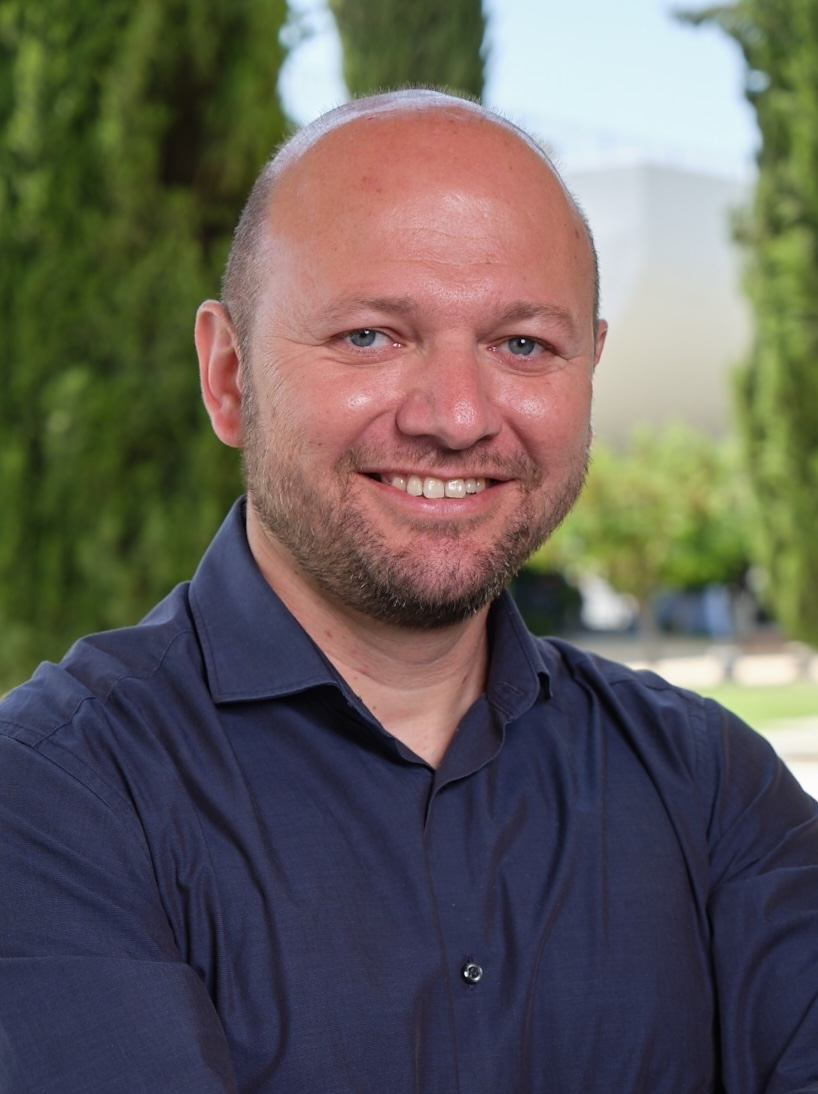
\includegraphics[width=1in,height=1.25in,clip,keepaspectratio]{figures/themis4-papers.jpg}}]{Themistoklis Charalambous}%%%
\DIFdelend \DIFaddbegin \begin{authorbiography}[{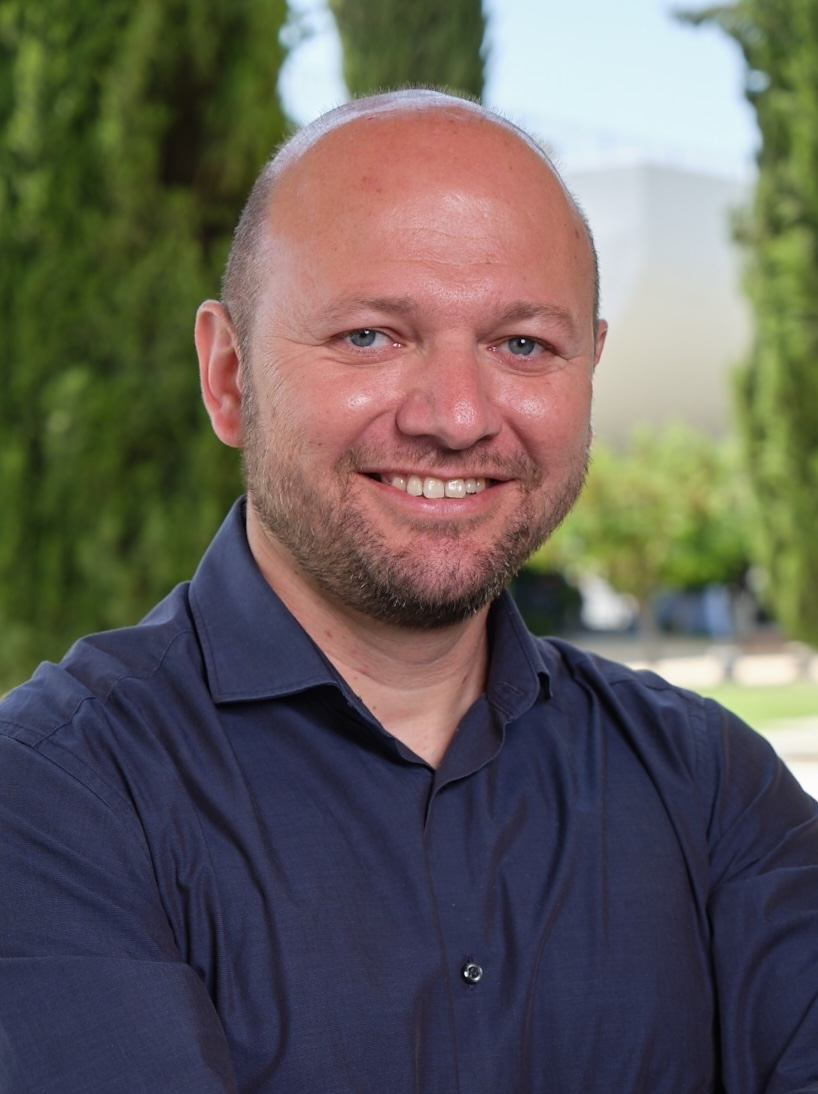
\includegraphics[width=\linewidth,height=1.25in,clip,keepaspectratio]{figures/themis4-papers.jpg}}]{Themistoklis Charalambous}\DIFaddend ~(Senior Member, IEEE) received the BA (First Class
Honours) and M.Eng. (Distinction) degrees in Electrical and Information Sciences from Trinity College, University of Cambridge, and the Ph.D. degree from the Control Laboratory, Department of Engineering, University of Cambridge.

Following his PhD, he held research and teaching positions at
Imperial College London, the University of Cyprus, KTH Royal Institute of Technology, and Chalmers University of Technology.

In 2017, he joined the Department of Electrical Engineering and Automation, School of Electrical Engineering, Aalto University, as an Assistant Professor; he was awarded the
title of Academy Research Fellow by the Academy of Finland in 2018 and was promoted to Associate Professor in 2020.

In September 2021, he joined the Department of Electrical and Computer Engineering, University of Cyprus, as a tenure-track Assistant Professor.
In May 2022, he received an ERC Consolidator Grant for the project ``MINERVA: Emerging Cooperative Autonomous Systems: Information for Control and Estimation.''
Since May 2026, he has been a tenured Associate Professor at the University of Cyprus. He is also a Visiting Professor at Aalto University and, since April 2023, at the FinEst Centre for Smart Cities.



\end{authorbiography}



\clearpage


\printindex

\end{document}
